\documentclass[11pt,a4paper,twoside,openright]{report}

\usepackage{fontspec}
\usepackage{shorttoc}%pour la réalisation d'un sommaire.

%\usepackage{hyperref}%rend actif les liens, références croisée, toc, ...
%		\hypersetup{colorlinks,%%
%		citecolor=black,%
%		filecolor=black,%
%		linkcolor=black,%
%		urlcolor=black} 

\usepackage[colorlinks = true,
	    linkcolor = blue,
            urlcolor  = blue,
            citecolor = blue,
            anchorcolor = blue]{hyperref}
\newcommand{\MYhref}[3][blue]{\href{#2}{\color{#1}{#3}}}%

\usepackage{textcomp}
\usepackage{animate}
\usepackage{tabularx}
\usepackage{colortbl}
\usepackage{makecell}
\renewcommand\theadfont{}
\usepackage[usenames,dvipsnames,table]{xcolor}
\definecolor{lightgray}{RGB}{218, 218, 218}
\definecolor{light-gray}{gray}{0.65}
\definecolor{cardinal}{RGB}{196, 30, 38}
\definecolor{bleu-info}{RGB}{218, 234, 238}
\definecolor{ocre-attention}{RGB}{238, 231, 218}
\definecolor{violet-question}{RGB}{226, 218, 238}
\definecolor{rouge-erreur}{RGB}{238, 218, 218}
\definecolor{gris-tab-entete}{RGB}{221, 221, 221}
\definecolor{gris-clair-tab}{RGB}{247, 247, 247}
\definecolor{gris-secret}{RGB}{238, 238, 238}

\usepackage[most]{tcolorbox}
\tcbuselibrary{minted, skins}

\newtcbox{mybox}{on line, fontupper=\scriptsize, arc=0pt,outer arc=0pt, colback=blue!5!white,
colframe=black!30!white, colupper=cardinal, boxsep=0pt,left=1pt,right=1pt,top=1pt,bottom=1pt,
boxrule=0.5pt,bottomrule=0.5pt,toprule=0.5pt}

\newtcolorbox{questionbox}{breakable, enhanced, arc=0mm, colback=violet-question, colframe=violet-question, leftrule=6mm,%
overlay={\node[anchor= west,outer sep=2pt] at (frame.west) {
\includegraphics[width=5mm]{images/question.png}}; }}

\newtcolorbox{attentionbox}{breakable, enhanced, arc=0mm, colback=ocre-attention, colframe=ocre-attention, leftrule=6mm,%
overlay={\node[anchor= west,outer sep=2pt] at (frame.west) {
\includegraphics[width=5mm]{images/attention.png}}; }}


\newtcolorbox{infobox}{breakable, enhanced, arc=0mm, colback=bleu-info, colframe=bleu-info,  leftrule=6mm,%
overlay={\node[anchor= west,outer sep=2pt] at (frame.west) {
\includegraphics[width=5mm]{images/info.png}}; }}

\newtcolorbox{erreurbox}{breakable, enhanced, arc=0mm, colback=rouge-erreur, colframe=rouge-erreur,  leftrule=6mm,%
overlay={\node[anchor= west,outer sep=2pt] at (frame.west) {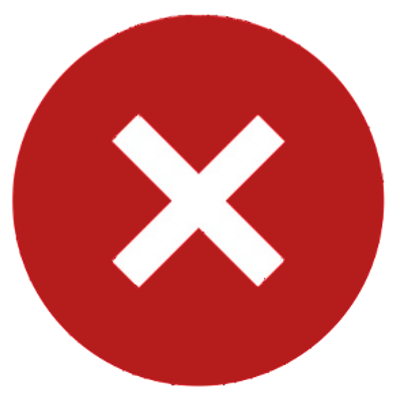
\includegraphics[width=5mm]{images/erreur.png}}; }}

\newtcolorbox{secretbox}{breakable, enhanced, arc=0mm, colback=gris-secret, colframe=gris-secret,  leftrule=6mm}


\usepackage{minted}
\newminted[bash]{bash}{
style = xcode,
autogobble,
frame=single,%
linenos,%
fontsize=\footnotesize%
%breaklines=true%
}
\newminted[C]{C}{
style=default,
autogobble,
frame=single,%
linenos,%
fontsize=\scriptsize%
%breaklines=true%
}


\usepackage[english,french]{babel}%pour un document en français
\usepackage[babel=true]{csquotes} % csquotes va utiliser la langue définie dans babel
\usepackage{graphicx}%pour insérer images et pdf entre autres
	\graphicspath{{images/}}%pour spécifier le chemin d'accès aux images
\usepackage{wrapfig}
\usepackage[left=2.5cm,right=2.5cm,top=2.5cm,bottom=2.5cm]{geometry}%réglages des marges du document selon vos préférences ou celles de votre établissement
\usepackage{array}
\usepackage{multirow}
\usepackage{lastpage}
\usepackage[Bjornstrup]{fncychap}%pour de jolis titres de chapitres voir la doc pour d'autres styles.
\usepackage{fancyhdr}%pour les entêtes et pieds de pages
	\setlength{\headheight}{14.2pt}% hauteur de l'entête
	
%%%%%%%%%%%%%%%%%%%style front%%%%%%%%%%%%%%%%%%%%%%%%%%%%%%%%%%%%%%%%%	
	\fancypagestyle{front}{%
  		\fancyhf{}%on vide les entêtes
  		\fancyfoot[C]{page \thepage}%
  		\renewcommand{\headrulewidth}{0pt}%trait horizontal pour l'entête
  		\renewcommand{\footrulewidth}{0.4pt}%trait horizontal pour les pieds de pages
		}


%%%%%%%%%%%%%%%%%%%style main%%%%%%%%%%%%%%%%%%%%%%%%%%%%%%%%%%%%
	\fancypagestyle{main}{%
		\fancyhf{}
  		\renewcommand{\chaptermark}[1]{\markboth{\chaptername\ \thechapter.\ ##1}{}}% redéfintion pour avoir ici les titres des chapitres des sections en minuscules
  		\renewcommand{\sectionmark}[1]{\markright{\thesection\ ##1}}
		\fancyhead[c]{}
		\fancyhead[RO,LE]{\rightmark}%
  		\fancyhead[LO,RE]{\leftmark}
		\fancyfoot[C]{}
		\fancyfoot[RO,LE]{\thepage}%
  		\fancyfoot[LO,RE]{https://zestedesavoir.com}
  		}

%%%%%%%%%%%%%%%%%%%style back%%%%%%%%%%%%%%%%%%%%%%%%%%%%%%%%%%%%%%%%%	
	\fancypagestyle{back}{%
  		\fancyhf{}%on vide les entêtes
  		\fancyfoot[C]{ \thepage}%
  		\renewcommand{\headrulewidth}{0pt}%trait horizontal pour l'entête
  		\renewcommand{\footrulewidth}{0.4pt}%trait horizontal pour les pieds de pages
		}


%%%%%%%%%%%%%%%%%%%%%%%%%%%%index%%%%%%%%%%%%%%%%%%%%%%%%%%%%%%%%%%%%%%%
\usepackage{makeidx}
\makeindex

%%%%%%%%%%%%%%%%%%%%%%%%%%%%%glossaire%%%%%%%%%%%%%%%%%%%%%%%%%%%%%%%%%%%
%\usepackage{glossaries}
%\makeglossaries		

%%%%%%%%%%%%%%%%%%%%%%%%%%%%liste des abbréviations%%%%%%%%%%%%%%		
%\usepackage[french]{nomencl}
%\makenomenclature
%\renewcommand{\nomname}{Liste des abréviation, des sigles et des symboles}



\begin{document}
%\frontmatter% début des pages liminaires
\pagestyle{front}%style des entêtes pour cette partie
%\thispagestyle{empty}
\phantomsection
\begin{titlepage}
\parindent=0pt
\begin{tikzpicture}[remember picture,overlay]
    \node[xshift=-0.5cm,yshift=-5.5cm] at (current page.90){%

\includegraphics[scale=0.7]{images/entete_ext.png}};
\end{tikzpicture}
\vspace*{9cm}
\begin{center}\sffamily\bfseries\LARGE
Auteurs :


    Lucas-84
    
    paraze
    
    Taurre
    
    informaticienzero
    
\end{center}

\vspace*{6cm}

\begin{center}\sffamily\bfseries\Large

Catégorie :

    Programmation et algorithmique 


Temps de lecture estimé : 1 jour et 6 heures
\end{center}

\vspace*{1cm}

\begin{center}\sffamily\bfseries\large
Licence CC 0
\end{center}

\end{titlepage}%on créé la couverture
\newpage
\thispagestyle{empty}%pour la page de garde toute blanche
\null
\newpage
\begin{titlepage}
\parindent=0pt

\vspace*{\stretch{1}}
\begin{center}\sffamily\bfseries\Huge
Le langage C
\end{center}

\vspace*{5cm}
\begin{center}\sffamily\bfseries\LARGE
Auteurs :

    Lucas-84
    
    paraze
    
    Taurre
    
    informaticienzero
    
\end{center}

\vspace*{6cm}

\begin{center}\sffamily\bfseries\Large

Catégorie :

    Programmation et algorithmique 


Temps de lecture estimé : 1 jour et 6 heures
\end{center}

\vspace*{1cm}

\begin{center}\sffamily\bfseries\large
Licence CC 0
\end{center}

\end{titlepage}%no comment!
\newpage
\thispagestyle{empty}%pour la page de garde toute blanche
\null
\newpage
\renewcommand{\abstractname}{Avant-propos}
\addcontentsline{toc}{chapter}{Avant-propos}\phantomsection
\begin{abstract}
Vous souhaitez apprendre à programmer, mais vous ne savez pas comment
vous y prendre ? Vous connaissez déjà le C, mais vous avez besoin de
revoir un certain nombre de points ? Ou encore, vous êtes curieux de
découvrir un nouveau langage de programmation ? Si oui, alors
permettez-nous de vous souhaiter la bienvenue dans ce cours de
programmation consacré au langage C.

Pour pouvoir suivre ce cours, aucun prérequis n’est nécessaire : tout
sera détaillé de la manière la plus complète possible, accompagné
d’exemples, d’exercices et de travaux pratiques.
\end{abstract}%no comment!
\renewcommand{\abstractname}{Remerciements}
\addcontentsline{toc}{chapter}{Remerciements} \phantomsection
\begin{abstract}
Avant de commencer, nous souhaitons remercier plusieurs personnes :
 \begin{itemize}

 \item Mewtow pour sa participation à la rédaction et à l’évolution de ce cours ainsi que pour ses nombreux conseils ;
 \item Arius et Saroupille pour la validation de ce cours ;
 \item Pouet\_forever, SofEvans, paraze et Mathuin pour leur soutien lors des débuts de la rédaction ;
 \item Dominus Carnufex pour son suivi minutieux et sa bienveillance face à nos (nombreuses) fautes de français ;
 \item Karnaj pour ses suggestions et corrections ;
 \item Maëlan pour sa relecture attentive du chapitre sur les encodages ;
 \item toute l’équipe de Progdupeupl et de Zeste de Savoir ;
 \item tous ceux qui, au fil du temps et de la rédaction, nous ont apporté leurs avis, leurs conseils, leurs points de vue et qui nous ont aidés à faire de ce cours ce qu’il est aujourd’hui ;
 \item et surtout vous, lecteurs, pour avoir choisi ce cours.

 \end{itemize}

\end{abstract}
%no comment!
\shorttableofcontents{Sommaire}{0}%sommaire avec uniquement les chapitres
\addcontentsline{toc}{chapter}{Sommaire}%ajout du sommaire dans le sommaire!


%\mainmatter% corps du document
\pagestyle{main}%style des entêtes pour cette partie
\part{Les bases du langage C}
\label{les-bases-du-langage-C}

\chapter{Introduction à la programmation}
\label{introduction-a-la-programmation}

La programmation est un sujet qui fascine énormément. Si vous lisez ce
cours, c’est que vous avez décidé de franchir le pas et de découvrir
de quoi il s’agit.  Cependant, avant de commencer à apprendre quoi que
ce soit sur le C et la programmation, il est d’abord nécessaire de
découvrir en quoi la programmation consiste. En effet, pour le moment,
vous ne savez pas réellement ce qu’est la programmation, ce que
signifie « programmer » ou encore ce qui caractérise le langage C. Ce
chapitre va donc consister en une introduction au monde de la
programmation, et plus particulièrement au langage C.

\section{Avant-propos}
\label{avant-propos}

\subsection{Esprit et but du tutoriel}
\label{esprit-et-but-du-tutoriel}

Ce cours a été écrit dans un seul but : vous enseigner le langage C de
la manière la plus complète, la plus rigoureuse et la plus instructive
possible. Pour ce faire, celui-ci combinera théorie, détails
techniques et exercices pratiques. Dès lors, nous ne vous le cachons
pas : cette approche va réclamer de votre part des \textbf{efforts},
certains passages étant assez complexes.

Nous avons choisi cette méthode d'apprentissage, car c'est celle que
nous jugeons la plus profitable. Elle s'oppose à une autre, plus
fréquente et plus superficielle, qui permet certes d'acquérir des
connaissances rapidement, mais qui s'avère bien souvent peu payante
sur le long terme.

En effet, beaucoup de programmeurs débutants se retrouvent ainsi
perdus lorsqu'ils sont jetés dans la jungle de la programmation à la
fin d'un cours, ceux-ci manquant souvent de connaissances techniques,
de (bonnes) pratique(s) et de rigueur.

Ne soyez toutefois pas apeuré, notre objectif n'est pas de vous noyer
d'informations ou de vous perdre avec des termes techniques. Nous vous
précisons simplement que ce cours nécessite d'avoir les doigts sur le
clavier et non dans le nez et que le début risque d'être un peu moins
« \emph{cool} » que ce que vous pourrez trouver ailleurs. ;)

\subsection{À qui est destiné ce cours ?}
\label{a-qui-est-destinuxe-ce-cours}

À n'importe quelle personne intéressée : que vous soyez un(e)
programmeur(euse) expérimenté(e), un(e) total(e) débutant(e) ou que
vous vouliez réviser certaines notions du C, vous êtes tous et toutes
les bienvenus(es). Les explications seront les plus claires possibles
afin de rendre la lecture accessible à tous.

Toutefois, quelques qualités sont opportunes pour arriver au bout de
ce cours :

\begin{itemize}
\item De la \textbf{motivation} : ce cours va présenter de nombreuses
  notions, souvent théoriques, et qui sembleront parfois complexes. Il
  vous faut donc être bien motivés pour profiter pleinement de cet
  apprentissage.
\item De la \textbf{logique} : apprendre la programmation, c'est aussi
  être logique. Bien sûr, ce cours vous apprendra à mieux l'être, mais
  il faut néanmoins savoir réfléchir par soi-même et ne pas compter
  sur les autres pour faire le travail à sa place.
\item De la \textbf{patience} : vous vous apprêtez à apprendre un
  langage de programmation. Pour arriver à un sentiment de maîtrise,
  il va vous falloir de la patience pour apprendre, comprendre, vous
  entraîner, faire des erreurs et les corriger.
\item De la \textbf{rigueur} : cette qualité, nous allons tenter de
  vous l'inculquer à travers ce cours. Elle est très importante, car
  c'est elle qui fera la différence entre un bon et un mauvais
  programmeur.
\item De la \textbf{curiosité} : n'hésitez pas à apporter des
  modifications aux codes proposés et à sortir un peu des balises du
  cours, cela ne vous sera que profitable.
\item De la \textbf{passion} : le plus important pour suivre ce
  tutoriel, c'est de prendre plaisir à programmer. Amusez-vous en
  codant, c'est le meilleur moyen de progresser !
\end{itemize}

À noter qu'un niveau acceptable en anglais est un plus indéniable,
beaucoup de cours, de forums et de documentations étant rédigés en
anglais. Si ce n'est pas le cas, gardez ceci à l'esprit : en
programmation, vous y serez confrontés tôt ou tard.

Enfin, un dernier point au sujet des mathématiques : contrairement à
la croyance populaire, un bon niveau en maths n'est absolument pas
nécessaire pour faire de la programmation. Certes, cela peut vous
aider en développant votre logique, mais si les mathématiques ne sont
pas votre fort, vous pourrez suivre ce cours sans problèmes.

\section{Aller plus loin}
\label{aller-plus-loin}

Un des concepts fondamentaux de l'apprentissage de notions
informatiques sur Internet est le \emph{croisement des sources}. Il
permet de voir la programmation sous un angle différent. Par exemple,
quelques cours de
\MYhref{http://c.developpez.com/cours/?page=lang-c}{Developpez}
recourant à des approches différentes sont à votre entière
disposition. N'hésitez pas non plus à lire des livres sur le C,
notamment le
\MYhref{http://en.wikipedia.org/wiki/The_C_Programming_Language}{K\&R},
écrit par les auteurs du langage (une version traduite en français est
disponible
\MYhref{http://www.dunod.com/informatique-multimedia/developpement/cc/ouvrages-denseignement/le-langage-c}{aux
  éditions Dunod}). C'est un livre qui pourra vous être utile.

\section{La programmation, qu’est-ce que c’est ?}
\label{la-programmation-quest-ce-que-cest}

\begin{infobox}
Dans cette section, nous nous
      contenterons d'une présentation succinte qui est suffisante pour
      vous permettre de poursuivre la lecture de ce cours. Toutefois,
      si vous souhaitez un propos plus étayé, nous vous conseillons la
      lecture du
      \MYhref{https://zestedesavoir.com/tutoriels/531/les-bases-de-la-programmation/}{cours
        d'introduction à la programmation} présent sur ce site.
\end{infobox}

La programmation est une branche de l'informatique qui sert à créer
des \textbf{programmes}. Tout ce que vous possédez sur votre
ordinateur est un programme : votre navigateur Internet (Internet
Explorer, Firefox, Opera, etc.), votre système d'exploitation
(Windows, GNU/Linux, Mac OS X, etc.) qui est un regroupement de
plusieurs programmes appelés \textbf{logiciels}, votre lecteur MP3,
votre logiciel de discussion instantanée, vos jeux vidéos, etc.

\subsection{Les programmes expliqués en long, en large et en   travers}
  \label{les-programmes-expliques-en-long-en-large-et-en-travers}

Un programme est une séquence d'\textbf{instructions}, d'ordres,
donnés à l'ordinateur afin qu'il exécute des actions. Ces instructions
sont généralement assez basiques. On trouve ainsi des instructions
d'addition, de multiplication, ou d'autres opérations mathématiques de
base, qui font que notre ordinateur est une vraie machine à calculer.
D'autres instructions plus complexes peuvent exister, comme des
opérations permettant de comparer des valeurs, traiter des caractères,
etc.

Créer un programme, c'est tout simplement utiliser une suite
d'instructions de base qui permettra de faire ce que l'on veut. Tous
les programmes sont créés ainsi : votre lecteur MP3 donne des
instructions à l'ordinateur pour écouter de la musique, le \emph{chat}
donne des instructions pour discuter avec d'autres gens sur le réseau,
le système d'exploitation donne des instructions pour dire à
l'ordinateur comment utiliser le matériel, etc.

\begin{infobox}
Notez qu'il n'est pas possible
    de créer des instructions. Ces dernières sont imprimées dans les
    circuits de l'ordinateur ce qui fait qu'il ne peut en gérer qu'un
    nombre précis et qu'il ne vous est donc pas loisible d'en
    construire de nouvelles (sauf cas particuliers vraiment tordus).
\end{infobox}

Notre ordinateur contient un composant électronique particulier,
spécialement conçu pour exécuter ces instructions : le
\textbf{processeur}. Ce qu'il faut retenir, c'est que notre ordinateur
contient un circuit, le processeur, qui permet d'effectuer de petits
traitements de base qu'on appelle des instructions et qui sont la base
de tout ce qu'on trouve sur un ordinateur.

Les instructions sont stockées dans notre ordinateur sous la forme de
chiffres binaires (appelés \emph{bits} en anglais), autrement dit sous
forme de zéros ou de uns. Ainsi, nos instructions ne sont rien d'autre
que des suites de zéros et de uns conservées dans notre ordinateur et
que notre processeur va interpréter comme étant des ordres à exécuter.
Ces suites de zéros et de uns sont difficilement compréhensibles pour
nous, humains, et parler à l'ordinateur avec des zéros et des uns est
très fastidieux et très long. Autant vous dire que créer des
programmes de cette façon revient à se tirer une balle dans le pied.

Pour vous donner un exemple, imaginez que vous deviez communiquer avec
un étranger alors que vous ne connaissez pas sa langue. Communiquer
avec un ordinateur reviendrait à devoir lui donner une suite de zéros
et de uns, ce dernier étant incapable de comprendre autre chose. Ce
langage s'appelle le \textbf{langage machine}.

Une question doit certainement vous venir à l'esprit : comment
communiquer avec notre processeur sans avoir à apprendre sa langue ?

L'idéal serait de parler à notre processeur en français, en anglais,
etc, mais disons-le clairement : notre technologie n'est pas
suffisamment évoluée et nous avons dû trouver autre chose. La solution
retenue a été de créer des langages de programmation plus évolués que
le langage machine, plus faciles à apprendre et de fournir le
traducteur qui va avec. Il s'agit de langages assez simplifiés,
souvent proches des langages naturels et dans lesquels on peut écrire
nos programmes beaucoup plus simplement qu'en utilisant le langage
machine. Grâce à eux, il est possible d'écrire nos programmes sous
forme de texte, sans avoir à se débrouiller avec des suites de zéros
et de uns totalement incompréhensibles. Il existe de nombreux langages
de programmation et l'un d'entre-eux est le \textbf{C}.

Reste que notre processeur ne comprend pas ces langages évolués et
n'en connaît qu'un seul : le sien. Aussi, pour utiliser un langage de
programmation, il faut disposer d'un traducteur qui fera le lien entre
celui-ci et le langage machine du processeur. Ainsi, il ne vous est
plus nécessaire de connaître la langue de votre processeur. En
informatique, ce traducteur est appelé un \textbf{compilateur}.

Pour illustrer notre propos, voici un code écrit en C (que nous
apprendrons à connaître).

\begin{C}
  #include <stdio.h>

  int main(void) { printf("Salut !\n"); return 0; }
\end{C}

\clearpage

Et le même en langage machine (plus précisémment pour un processeur de
la famille x86-64).

\begin{C}
  01010101 01001000 10001001 11100101 10111111 00100100 00101100
  01001000 00000000 10111000 00000000 00000000 00000000 00000000
  11101000 10011101 00001011 00000000 00000000 10111000 00000000
  00000000 00000000 00000000 01011101 11000011 01010011 01100001
  01101100 01110101 01110100 00100000 00100001 00001010 00000000
\end{C}

Nous y gagnons tout de même au change, non ? :pMalgré tous ces
langages de programmation disponibles nous allons, dans ce tutoriel,
nous concentrer sur un seul d'entre-eux : le C. Avant de parler des
caractéristiques de ce langage et des choix qui nous amènent à
l'étudier dans ce cours, faisons un peu d'histoire.

\section{Le langage C}
\label{le-langage-C}

\subsection{L'histoire du C}
\label{lhistoire-du-c}

Le langage C est né au début des années 1970 dans les laboratoires de
la société AT\&T aux États-Unis. Son concepteur,
\MYhref{http://fr.wikipedia.org/wiki/Dennis_Ritchie}{Dennis MacAlistair
  Ritchie}, souhaitait améliorer un langage existant, le B, afin de
lui adjoindre des nouveautés. En 1973, le C était pratiquement au
point et il commença à être distribué l'année suivante. Son succès fut
tel auprès des informaticiens qu'en 1989, l'ANSI, puis en 1990, l'ISO,
décidèrent de le normaliser, c'est-à-dire d'établir des règles
internationales et officielles pour ce langage. À l'heure actuelle, il
existe trois normes : la norme ANSI C89 ou ISO C90, la norme ISO C99
et la norme ISO C11.

\emph{{[}AT\&T{]}: American Telephone and Telegraph Company
}{[}ANSI{]}: American National Standards Institute *{[}ISO{]}:
International Organization for Standardization

\begin{infobox}
Si vous voulez en savoir plus sur
l'histoire du C, lisez donc
\MYhref{http://c.developpez.com/cours/historique-langage-c/}{ce
  tutoriel}.
\end{infobox}

\subsection{Pourquoi apprendre le C ?}
\label{pourquoi-apprendre-le-c}

C'est une très bonne question. :D Après tout, étant donné qu'il existe
énormément de langages différents, il est légitime de se demander
pourquoi choisir le C en particulier ? Il y a plusieurs raisons à
cela.

\begin{itemize}
\item Sa \textbf{popularité} : le C fait partie des langages de
  programmation les plus utilisés. Il possède une communauté très
  importante, de nombreux cours et beaucoup de documentations. Vous
  aurez donc toujours du monde pour vous aider. De plus, il existe un
  grand nombre de programmes et de bibliothèques développés en C.
\item Sa \textbf{rapidité} : le C est connu pour être un langage très
  rapide, ce qui en fait un langage de choix pour tout programme où la
  vitesse d'exécution est cruciale.
\item Sa \textbf{simplicité} : le C est un langage minimaliste pourvu
  de peu de concepts ce qui permet d'en faire le tour
  \emph{relativement} rapidement et d'éviter un niveau d'abstraction
  trop important.
\item Sa \textbf{légèreté} : le C est léger, ce qui le rend utile pour
  les programmes embarqués où la mémoire disponible est faible.
\item Sa \textbf{portabilité} : cela signifie qu'un programme
  développé en C peut être compilé pour fonctionner sur différentes
  machines sans devoir changer ledit code.
\end{itemize}

Ce ne sont que quelques raisons, mais elles sont à notre goût
suffisantes pour justifier l'apprentissage de ce langage. Bien
entendu, le C comporte aussi sa part de défauts. On peut citer la
tolérance aux comportements dangereux qui fait que le C demande de la
rigueur pour ne pas tomber dans certains « pièges », un nombre plus
restreint de concepts (c'est parfois un désavantage, car on est alors
obligé de recoder certains mécanismes qui existent nativement dans
d'autres langages), etc. D'ailleurs, si votre but est de développer
rapidement des programmes amusants, sachez que le C n'est pas adapté
pour cela et que nous vous conseillons, dans ce cas, de vous tourner
vers d'autres langages, comme par exemple le
\MYhref{https://zestedesavoir.com/tutoriels/799/apprendre-a-programmer-avec-python-3/}{Python}
ou le
\MYhref{https://zestedesavoir.com/tutoriels/634/une-introduction-a-ruby/}{Ruby}.

Le C possède aussi une caractéristique qui est à la fois un avantage et
un défaut : il s'agit d'un langage dit de « \textbf{bas niveau} ». Cela
signifie qu'il permet de programmer en étant « proche de sa machine »,
c'est-à-dire sans trop vous cacher son fonctionnement interne. Cette
propriété est à double tranchant : d'un côté elle rend l'apprentissage
plus difficile et augmente le risque d'erreurs ou de comportements
dangereux, mais de l'autre elle vous laisse une grande liberté d'action
et vous permet d'en apprendre plus sur le fonctionnement de votre
machine. Cette notion de « bas niveau » est d'ailleurs à opposer aux
langages dit de « \textbf{haut niveau} » qui permettent de programmer en
faisant abstraction d'un certain nombre de choses. Le développement est
rendu plus facile et plus rapide, mais en contrepartie, beaucoup de
mécanisme interne sont cachés et ne sont pas accessibles au programmeur.
Ces notions de haut et de bas niveau sont néanmoins à nuancer, car elles
dépendent du langage utilisé et du point de vue du programmeur (par
exemple, par rapport au langage machine, le C est un langage de haut
niveau).

Une petite note pour terminer : peut-être avez-vous entendu parler du
\textbf{C++} ? Il s'agit d'un langage de programmation qui a été inventé
dans les années 1980 par
\MYhref{https://en.wikipedia.org/wiki/Bjarne_Stroustrup}{Bjarne
Stroustrup}, un collègue de Dennis Ritchie, qui souhaitait rajouter des
éléments au C. Bien qu'il fût très proche du C lors de sa création, le
C++ est aujourd'hui un langage très différent du C et n'a pour ainsi
dire plus de rapport avec lui (si ce n'est une certaine proximité au
niveau d'une partie de sa syntaxe). Ceci est encore plus vrai en ce qui
concerne la manière de programmer et de raisonner qui sont
\emph{radicalement} différentes.

Ne croyez toutefois pas, comme peut le laisser penser leur nom ou leur
date de création, qu'il y a un langage meilleur que l'autre, ils sont
simplement \emph{différents}. Si d'ailleurs votre but est d'apprendre le
C++, nous vous encourageons à le faire. En effet, contrairement à ce qui
est souvent dit ou lu, \emph{il n'y a pas besoin de connaitre le C pour
apprendre le C++}.

\section{La norme}
\label{la-norme}

Comme précisé plus haut, le C est un langage qui a été normalisé à trois
reprises. Ces normes servent de référence à tous les programmeurs et les
aident chaque fois qu'ils ont un doute ou une question en rapport avec
le langage. Bien entendu, elle ne sont pas parfaites et ne répondent pas
à toutes les questions, mais elles restent \emph{la} référence pour tout
programmeur.

Ces normes sont également indispensables pour les compilateurs. En
effet, le respect de ces normes par les différents compilateurs permet
qu'il n'y ait pas de différences d'interprétation d'un même code.
Finalement, ces normes sont l'équivalent de nos règles d'orthographe, de
grammaire et de conjugaison. Imaginez si chacun écrivait ou conjuguait à
sa guise, ce serait un sacré bazar\ldots{}

Dans ce cours, nous avons décidé de nous reposer sur la norme ANSI C89
(ou ISO C90, c'est pareil). En effet, même s'il s'agit de la plus
ancienne, elle nous permettra néanmoins de développer avec n'importe
quel compilateur et sous n'importe quel système sans problèmes et sans
nous poser de questions sur la présence ou non de telle ou telle
fonctionnalité.

Rassurez-vous néanmoins : le fait de nous baser sur la norme C89 ne
signifie pas que vous allez découvrir une version obsolète du langage C.
En effet, d'une part, ce que vous allez voir tout au long de ce cours
est toujours valable au regard des normes plus récentes et, d'autre
part, les changements induits par les autres normes sont le plus souvent
mineurs et consistent pour ainsi dire tous en des \emph{ajouts} et non
en des modifications. De ce fait, il vous sera aisé, une fois ce cours
parcouru, de passer à une norme plus récente.

\begin{infobox} Pour les curieux, voici
    \MYhref{http://flash-gordon.me.uk/ansi.c.txt}{un lien} vers le
    brouillon de cette norme. Cela signifie qu'il ne s'agit pas de la
    version définitive et officielle, cependant il est largement
    suffisant pour notre niveau et, surtout, il est gratuit (la norme
    officielle coûtant \emph{très} cher :-° ). Notez que celui-ci est
    rédigé en anglais
\end{infobox}

\section{L’algorithmique}
\label{l-algorithmique}

L'algorithmique est liée à la programmation et constitue même une
branche à part des mathématiques.  Elle consiste à définir et établir
des \textbf{algorithmes}.

Un algorithme peut se définir comme étant une suite finie et
non-ambiguë d'opérations permettant de résoudre un problème. En clair,
il s'agit de calculs qui prennent plusieurs paramètres et fournissent
un résultat.  Les algorithmes ne sont pas limités à l'informatique,
ils existaient même avant son apparition ; prenez les recettes de
cuisine par exemple, ou des instructions de montage d'un meuble ou
d'un Lego, ce sont des algorithmes.

L'intérêt principal des algorithmes est qu'ils sont très utiles
lorsqu'ils sont en relation avec des ordinateurs. En effet, ces
derniers peuvent exécuter des milliards d'instructions à la seconde,
ce qui les rend bien plus rapides qu'un humain. Illustrons : imaginez
que vous deviez trier une liste de dix nombres dans l'ordre
croissant. C'est assez facile et faisable en quelques secondes. Et
pour plusieurs milliards de nombres ? C'est impossible pour un humain,
alors qu'un ordinateur le fera rapidement.

Ce qu'il faut retenir, c'est qu'un algorithme est une suite
d'opérations destinée à résoudre un problème donné. Nous aurons
l'occasion d'utiliser quelques algorithmes dans ce cours, mais nous ne
nous concentrerons pas dessus.

\fbox{\begin{minipage}{0.9\textwidth}Si vous voulez en savoir plus,
    lisez le tutoriel sur
    \MYhref{/tutoriels/621/algorithmique-pour-lapprenti-programmeur/}{l'algorithmique
      pour l'apprenti programmeur} en même temps que vous apprenez à
    programmer avec celui-ci.
  \end{minipage}}

\subsection{Le pseudo-code}
\label{le-pseudo-code}

Pour représenter un algorithme indépendamment de tout langage, on
utilise ce qu'on appelle un \textbf{pseudo-code}. Il s'agit de la
description des étapes de l'algorithme en langage naturel (dans notre
cas le français). Voici un exemple de pseudo-code.

\begin{C}
  Fonction max (x, y)
    
  Si x est supérieur à y Retourner x Sinon Retourner y

  Fin fonction
\end{C}

Dans ce cours, il y aura plusieurs exercices dans lesquels un
algorithme fourni devra être mis en œuvre, traduit en C. Si vous
voulez vous entrainer davantage tout en suivant ce cours, nous vous
conseillons \MYhref{http://www.france-ioi.org/}{France-IOI} qui permet
de mettre en application divers algorithmes dans plusieurs langages,
dont le C. Cela pourra être un excellent complément.

\hrulefill

Comme vous avez pu le constater, la programmation est un monde vaste,
très vaste, et assez complexe. Comme il existe une multitude de
langages de programmation, il faut se concentrer sur un seul d'entre
eux à la fois. Dans notre cas, il s'agit du C. Ce langage, et
retenez-le bien, est à la fois puissant et complexe. Rappelez-vous
bien qu'il vous faudra faire des efforts pour l'apprendre
correctement.

Si vous vous sentez prêts, alors rendez-vous dans le chapitre suivant,
qui vous montrera les outils utilisés par un programmeur C.
\chapter{Rencontre avec le C}

Maintenant que les présentations sont faites, il est temps de
découvrir les outils nécessaires pour programmer en C. Le strict
minimum pour programmer se résume en trois points :

\begin{itemize}

\item un \textbf{éditeur de texte} (à ne pas confondre avec un
  \textbf{traitement de texte} comme \emph{Microsoft Word} ou
  \emph{LibreOffice Writer}) : ce logiciel va servir à l'écriture du
  code source. Techniquement, n'importe quel éditeur de texte suffit,
  mais il est souvent plus agréable d'en choisir un qui n'est pas trop
  minimaliste ;
\item
  un \textbf{compilateur} : c'est le logiciel le plus important
  puisqu'il va nous permettre de transformer le code écrit en langage C
  en un fichier exécutable ;
\item un \textbf{débogueur} (ou \emph{debugger} en anglais) : ce
  logiciel vous sera très utile en cas de problèmes pour rechercher
  d'éventuelles erreurs dans votre programme.
\end{itemize}

À partir de là, il existe deux solutions : utiliser ces trois
logiciels séparément ou bien les utiliser au sein d'un
\textbf{environnement intégré de développement} (abrégé EDI). Dans le
cadre de ce cours, nous avons choisi la première option,
majoritairement dans un souci de transparence et de simplicité. En
effet, si les EDI peuvent être des compagnons de choix, ceux-ci sont
avant tout destinés à des programmeurs expérimentés et non à de
parfaits débutants

\section{Windows} 

\subsection{Le compilateur}

Nous vous proposons de télécharger MinGW, qui est une adaptation pour
Windows du compilateur GCC.

Rendez-vous sur le \MYhref{http://www.mingw.org/}{site de MinGW} dans
la section « \emph{download} » et cliquez sur le lien en haut de la
page « \emph{looking for the latest version ? Download
  mingw-get-install-xxxxxxxx.exe (xxx.x kB)} ».

Exécutez le programme, cliquez sur « \emph{install} », décochez la
case « \emph{also install support for graphical user interface} » et
enfin cliquez sur « \emph{continue} ».

Ceci étant fait, il nous faut désormais créer une variable
d'environnement afin de spécifier à notre invite de commande le chemin
vers les différents composants de MinGW.

\begin{itemize}
\item sous Windows XP et antérieur, faites un clic-droit sur « poste
  de travail » puis choisissez « propriétés ». Dans la fenêtre qui
  s'ouvre, cliquez sur « avancés » puis sur « variables
  d'environnement » ;
\item sous Windows Vista, Seven, faites un clic-droit sur l'icône «
  ordinateur » dans le menu « démarrer » ou bien sur « poste de
  travail ». Ensuite, cliquez sur « paramètres systèmes avancés
  ». Dans la nouvelle fenêtre qui s'ouvre, cliquez sur « variables
  d'environnement » ;
\item sous Windows 8, rendez-vous dans le panneau de configuration à
  la rubrique « système ». Cliquez sur « avancé » puis sur « variables
  d'environnement ».
\end{itemize}

\bigbreak

Dans la partie « utilisateur courant », créez une nouvelle variable
nommée \mybox{PATH} et donnez lui pour valeur :
\mybox{\%PATH\%;C:\textbackslash{}MinGW\textbackslash{}bin} (le chemin
après le point-virgule peut varier en fonction de où vous avez décidés
d'installer MinGW, l'important est de bien avoir le répertoire
\mybox{bin} à la fin).

À présent, exécutez l'invite de commandes (il est situé dans les
accessoires sous le même nom) et entrez la ligne suivante.

\begin{bash}
  mingw-get install gcc gdb
\end{bash}

Le compilateur et le débogueur sont à présent installés. À présent,
lancez le bloc-note et placez y le texte suivant.

\begin{bash}
  @echo off gcc -D__USE_MINGW_ANSI_STDIO=1 -Wall -Wextra -pedantic -std=c89 -fno-common
    -fno-builtin %*
\end{bash}

Ensuite, enregistrez ce fichier dans le dossier « bin » de MinGW (par
défaut \mybox{C:\textbackslash{}MinGW\textbackslash{}bin}) sous le nom
« zcc.bat » en choisissant « autres types de fichiers ».

Maintenant, rendez-vous dans le menu des accessoires, réalisez un clic
droit sur l'invite de commande et sélectionnez « propriétés ». Dans
l'onglet « raccourci », remplacer le champ « cible » par
«\%windir\%\textbackslash system32\textbackslash cmd.exe /k ``chcp
65001'' ». Enfin, dans l'onglet « police », choisissez « Consolas » ou
« Lucida Console » et adaptez la taille suivant vos envies.

\section{L'éditeur de texte}\label{luxe9diteur-de-texte-1}

L'éditeur de texte va nous permettre d'écrire notre code source et de
l'enregistrer. L'idéal est d'avoir un éditeur de texte facile à
utiliser et pas trop minimaliste. Si jamais vous avez déjà un éditeur
de texte et que vous l'appréciez, n'en changez pas, il fera sûrement
l'affaire.

Si vous n'avez pas d'idée, nous vous conseillons
\MYhref{http://notepad-plus-plus.org/fr/}{Notepad++} qui est simple,
pratique et efficace. Pour le télécharger, rendez-vous simplement dans
la rubrique « Téléchargements » du menu principal.

\begin{infobox}
 Veillez-bien à ce que l'encodage de
votre fichier soit « UTF-8 (sans BOM) » (voyez le menu éponyme à cet
effet).
\end{infobox}

\section{Introduction à la ligne de
  commande}\label{introduction-uxe0-la-ligne-de-commande-1}

La ligne de commande, derrière son aspect rustre et archaïque, n'est
en fait qu'une autre manière de réaliser des tâches sur un
ordinateur. La différence majeure avec une interface graphique étant
que les instructions sont données non pas à l'aide de boutons et de
cliques de souris, mais exclusivement à l'aide de texte. Ainsi, pour
réaliser une tâche donnée, il sera nécessaire d'invoquer un programme
(on parle souvent de \textbf{commandes}) en tapant son nom.

La première chose que vous devez garder à l'esprit, c'est le dossier
dans lequel vous vous situez. Celui-ci est indiqué au tout début de
chaque ligne et se termine par le symbole \mybox{\textgreater{}}. Ce
dossier est celui dans lequel les actions (par exemple la création
d'un répertoire) que vous demanderez seront réalisées. Normalement,
par défaut, vous devriez vous situez dans le répertoire
\mybox{C:\textbackslash{}Users\textbackslash{}Utilisateur} (où
\mybox{Utilisateur} correspond à votre nom d'utilisateur). Ceci étant
posé, voyons quelques commandes basiques.

La commande \mybox{mkdir} (pour \emph{make directory}) vous permet de
créer un nouveau dossier. Pour ce faire, tapez \mybox{mkdir} suivi
d'un espace et du nom du nouveau répertoire. Par exemple, vous pouvez
créer un dossier « Programmation » comme suit.

\begin{bash}
  C:\Users\Utilisateur> mkdir Programmation
\end{bash}

La commande \mybox{dir} (pour \emph{directory}) vous permet de lister
le contenu d'un dossier. Vous pouvez ainsi vérifier qu'un nouveau
répertoire a bien été créé.

\begin{bash}
  C:\Users\Utilisateur> dir Répertoire de C:\Users\Utilisateur

  30/03/2015 17:00 <REP> .  30/03/2015 17:00 <REP> ..  30/03/2015
  17:00 <REP> Programmation
\end{bash}

\begin{infobox}
  Le résultat ne sera pas forcément le même que ci-dessus, cela dépend
  du contenu de votre dossier. L'essentiel est que vous retrouviez
  bien le dossier que vous venez de créer.
\end{infobox}

Enfin, la commande \mybox{cd} (pour \emph{change directory}) vous
permet de vous déplacer d'un dossier à l'autre. Pour ce faire,
spécifiez simplement le nom du dossier de destination.

\begin{bash}
  C:\Users\Utilisateur> cd Programmation
  C:\Users\Utilisateur\Programmation>
\end{bash}

\begin{infobox}
Le dossier spécial « \textbf{..} »
représente le répertoire parent. Il vous permet donc de revenir en
arrière dans la hiérarchie des dossiers. Le dossier spécial «
\textbf{.}  » représente quant à lui le dossier courant.
\end{infobox}

Voilà, avec ceci, vous êtes fin prêt pour compiler votre premier
programme. Vous pouvez vous rendre à la deuxième partie de ce
chapitre.

\emph{{[}MinGW{]}: Minimalist GNU for Windows }{[}GCC{]}: GNU Compiler
Collection.

\section{GNU/Linux, *BSD et autres Unixoïdes}

\subsection{ Le compilateur}\label{le-compilateur}

Suivant le système que vous choisissez, vous aurez ou non le choix
entre différents compilateurs. Si vous n'avez pas d'idée, nous vous
conseillons d'opter pour GCC en installant le paquet éponyme à l'aide
de votre gestionnaire de paquet. Également, vous pouvez installer le
paquet « gdb » qui est un débogueur.

\subsection{Configuration}\label{configuration-1}

Ceci dépend de votre interpréteur de commande. Pour savoir quel est
celui dont vous disposez, ouvrez un terminal (le plus souvent, vous
pouvez y accéder via la catégorie « accessoires » de votre menu
principal) et entrez la commande suivante.

\begin{bash}
  echo $SHELL
\end{bash}


\subsubsection{bash}\label{bash}

Exécutez la commande suivante depuis votre dossier personnel (vous y
êtes par défaut au lancement de l'invite de commande).

\begin{bash}
  echo "alias zcc='gcc -Wall -Wextra -pedantic -std=c89 -fno-common -fno-builtin'"
  >> .bashrc
\end{bash}


\subsubsection{csh ou tcsh}\label{csh-ou-tcsh}

Exécutez la commande suivante depuis votre dossier personnel (vous y
êtes par défaut au lancement de l'invite de commande).

\begin{bash}
  echo "alias zcc 'gcc -Wall -Wextra -pedantic -std=c89 -fno-common -fno-builtin'"
  >> .cshrc # (ou .tcshrc)
\end{bash}


\subsubsection{ksh, zsh ou sh}\label{ksh-zsh-ou-sh}

Exécutez les commandes suivante depuis votre dossier personnel (vous y
êtes par défaut au lancement de l'invite de commande).

\begin{bash}
  echo "alias zcc='gcc -Wall -Wextra -pedantic -std=c89 -fno-common -fno-builtin'"
  >> .kshrc # (ou .zshrc ou .shrc) echo "export ENV=\$HOME.kshrc"
  >> .profile # (ou .zshrc ou .shrc)
\end{bash}

\subsection{L'éditeur de texte}\label{luxe9diteur-de-texte-2}

Ce serait un euphémisme de dire que vous avez l'embarras du choix. Il
existe une pléthore d'éditeurs de texte fonctionnant en ligne de
commande ou avec une interface graphique, voire les deux.

Pour n'en citer que quelques-uns, en ligne de commande vous trouverez
par exemple : Vim et Emacs (les deux monstres de l'édition), Nano ou
Joe. Côté graphique, vous avez entre autres : Gedit, Mousepad et Kate.

\subsection{Introduction à la ligne de
  commande}\label{introduction-uxe0-la-ligne-de-commande-2}

La ligne de commande, derrière son aspect rustre et archaïque, n'est
en fait qu'une autre manière de réaliser des tâches sur un
ordinateur. La différence majeure avec une interface graphique étant
que les instructions sont données non pas à l'aide de boutons et de
cliques de souris, mais exclusivement à l'aide de texte. Ainsi, pour
réaliser une tâche donnée, il sera nécessaire d'invoquer un programme
(on parle souvent de \textbf{commandes}) en tapant son nom.

La première chose que vous devez garder à l'esprit, c'est le dossier
dans lequel vous vous situez. Suivant le terminal que vous employez,
celui-ci est parfois indiqué en début de ligne et terminé par le
symbole \mybox{\$} ou \mybox{\%}. Ce dossier est celui dans lequel les
actions (par exemple la création d'un répertoire) que vous demanderez
seront exécutées. Normalement, par défaut, vous devriez vous situez
dans le répertoire : \mybox{/home/utilisateur} (où \mybox{utilisateur}
correspond à votre nom d'utilisateur). Ceci étant posé, voyons
quelques commandes basiques.

La commande \mybox{pwd} (pour \emph{print working directory}) vous
permet de connaître le répertoire dans lequel vous êtes.

\begin{bash}
  $ pwd /home/utilisateur
\end{bash}

La commande \mybox{mkdir} (pour \emph{make directory}) vous permet de
créer un nouveau dossier. Pour ce faire, tapez \mybox{mkdir} suivi
d'un espace et du nom du nouveau répertoire. Par exemple, vous pouvez
créer un dossier « programmation » comme suit :

\begin{bash}
  $ mkdir programmation
\end{bash}

La commande \mybox{ls} (pour \emph{list}) vous permet de lister le
contenu d'un dossier. Vous pouvez ainsi vérifier qu'un nouveau
répertoire a bien été créé.

\begin{bash}
  $ ls programmation
\end{bash}

\begin{infobox}
  Le résultat ne sera pas forcément le même que ci-dessus, cela dépend
  du contenu de votre dossier. L'essentiel est que vous retrouviez
  bien le dossier que vous venez de créer.
\end{infobox}

Enfin, la commande \mybox{cd} (pour \emph{change directory}) vous
permet de vous déplacer d'un dossier à l'autre. Pour ce faire,
spécifiez simplement le nom du dossier de destination.

\begin{bash}
  $ cd programmation 
  $ pwd /home/utilisateur/programmation
\end{bash}

\begin{infobox}
Le dossier spécial « \textbf{..} »
représente le répertoire parent. Il vous permet donc de revenir en
arrière dans la hiérarchie des dossiers. Le dossier spécial «
\textbf{.}  » représente quant à lui le dossier courant.
\end{infobox}

Voilà, avec ceci, vous êtes fin prêt pour compiler votre premier
programme. Vous pouvez vous rendre à la deuxième partie de ce
chapitre.

*{[}GCC{]}: GNU Compiler Collection

\section{Mac OS X}

\subsection{Le compilateur}

Allez dans le dossier \mybox{/Applications/Utilitaires} et lancez
l'application « terminal.app ». Une fois ceci fait, entrez la commande
suivante :

\begin{bash}
xcode-select --install
\end{bash}

et cliquez sur « installer » dans la fenêtre qui apparaît. Si vous
rencontrez le message d'erreur ci-dessous, cela signifie que vous
disposez déjà des logiciels requis.

\begin{bash}
  Impossible d’installer ce logiciel car il n’est pas disponible
  actuellement depuis le serveur de mise à jour de logiciels.
\end{bash}

Si vous ne disposez pas de la commande indiquée, alors rendez-vous sur
le site de développeur d'Apple :
\MYhref{https://developer.apple.com/}{\emph{Apple developer
    connection}}.  Il faudra ensuite vous rendre sur le « \emph{mac
  dev center} » puis, dans « \emph{additional download} », cliquez sur
« \emph{view all downloads} ». Quand vous aurez la liste, il vous
suffit de chercher la version 3 de Xcode (pour Leopard et Snow
Leopard) ou 2 pour les versions antérieures (Tiger). Vous pouvez aussi
utiliser votre CD d'installation pour installer Xcode (sauf pour
Lion).

\subsection{Configuration}\label{configuration}

Voyez ce qui est dit pour GNU/Linux, *BSD et les autres Unixoïdes.

\subsection{L'éditeur de texte}\label{luxe9diteur-de-texte}

Comme pour les autres Unixoïdes, vous trouverez un bon nombres
d'éditeurs de texte. Si toutefois vous êtes perdu, nous vous
conseillons
\MYhref{http://www.barebones.com/products/TextWrangler/}{TextWrangler}
ou \MYhref{https://www.peterborgapps.com/smultron/}{Smultron}.

\subsection{Introduction à la ligne de
commande}\label{introduction-uxe0-la-ligne-de-commande}

Référez-vous à l'introduction dédiée à GNU/Linux, *BSD et les autres
Unixoïdes.

\section{Notre cible}

Avant de commencer à programmer, il nous faut aussi définir ce que
nous allons programmer, autrement dit le type de programme que nous
allons réaliser. Il existe en effet deux grands types de programmes :
les programmes \textbf{graphiques} et les programmes \textbf{en
  console}.

Les programmes graphiques sont les plus courants et les plus connus
puisqu'il n'y a pratiquement qu'eux sous Windows ou Mac OS X par
exemple. Vous en connaissez sans doute énormément tel que les lecteurs
de musique, les navigateurs Internet, les logiciels de discussions
instantanées, les suites bureautiques, les jeux vidéos, etc. Ce sont
tous des programmes graphiques, ou programmes GUI. En voici un exemple
sous GNU/Linux.

\begin{figure}[!ht]
\centering
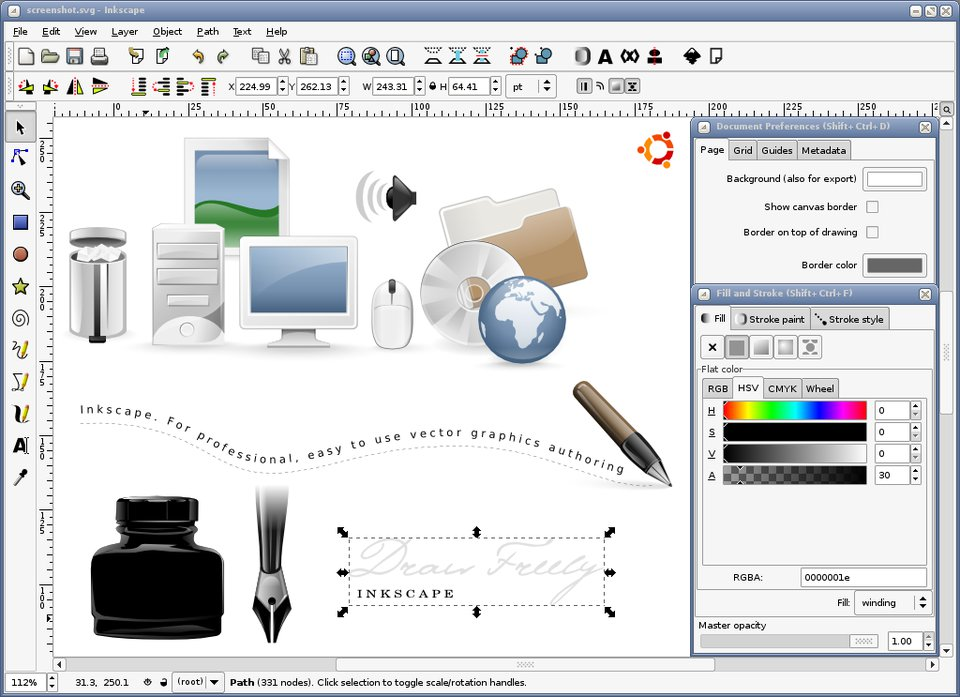
\includegraphics[scale=0.4]{images/Inskape_screenshot.jpg}
\caption{L'éditeur d'images vectorielles Inkscape est un programme
graphique}
\end{figure}

Cependant, écrire ce genre de programmes demande beaucoup de
connaissances, ce qui nous manque justement pour l'instant. Aussi,
nous allons devoir nous rabattre sur le deuxième type de programme :
les programmes en console.

Les programmes console sont les premiers programmes et sont apparus en
même temps que l'écran. Ils étaient très utilisés dans les années
1970/1980 (certains d'entre vous se souviennent peut-être de MS-DOS),
mais ont fini par être remplacés par une interface graphique avec la
sortie de Mac OS et de Windows. Cependant, ils existent toujours et
redeviennent quelque peu populaires chez les personnes utilisant
GNU/Linux ou un *BSD.

Voici un exemple de programme en console (il s'agit de
\MYhref{http://www.gnu.org/software/chess/}{GNU Chess}, un jeu
d'échecs performant entièrement en ligne de commande).

\begin{bash}
White (1) : d4
1. d4

black  KQkq  d3
r n b q k b n r 
p p p p p p p p 
. . . . . . . . 
. . . . . . . . 
. . . P . . . . 
. . . . . . . . 
P P P . P P P P 
R N B Q K B N R 

Thinking...

white  KQkq
r n b q k b . r 
p p p p p p p p 
. . . . . n . . 
. . . . . . . . 
. . . P . . . . 
. . . . . . . . 
P P P . P P P P 
R N B Q K B N R 


My move is : Nf6
White (2) :
\end{bash}

Ce sera le type de programme que nous allons apprendre à créer.
Rassurez-vous, quand vous aurez fini le cours, vous aurez les bases
pour apprendre à créer des programmes graphiques. Tout est possible.

\section{Première rencontre}

Bien, il est à présent temps d'écrire et de compiler notre premier
programme ! Pour ce faire, ouvrez votre éditeur de texte et entrez les
lignes suivantes.

\begin{C}
  int main(void)
  {
    return 0
  }
\end{C}

Ensuite, enregistrez ce fichier dans un dossier de votre choix et
nommez-le « main.c ». Une fois ceci fait, rendez-vous dans le dossier
contenant le fichier à l'aide d'un terminal et exécutez la commande
ci-dessous.

\begin{C}
zcc main.c
\end{C}

\clearpage

\begin{attentionbox}
  Si vous n'êtes pas sous Windows et que vous utilisez
  l'interprétateur de commande \mybox{sh}, \mybox{ksh} ou \mybox{zsh},
  la commande \mybox{zcc} ne sera connue de votre invite de commande
  qu'une fois que vous aurez ouvert une nouvelle session. En
  attendant, vous pouvez entrez la commande \mybox{alias zcc='gcc
    -Wall -Wextra -pedantic -std=c89 -fno-common -fno-builtin'} dans
  votre terminal pour que cela fonctionne.
\end{attentionbox}

Si tout se passe bien, vous devriez obtenir un fichier « a.exe » sous
Windows et un fichier « a.out » sinon. Vous pouvez exécutez ce programme
en tapant \mybox{a.exe} ou \mybox{./a.out}.

\begin{questionbox}
  Je viens de le faire, mais il ne se passe rien
\end{questionbox}


Cela tombe bien, c'est exactement ce que fait ce programme : rien. :p
Voyons cela plus en détails.

Ce bout de code est appelé une \textbf{fonction}. Un programme écrit en
C n'est composé pratiquement que de fonctions qui sont des morceaux de
programme donnant des instructions à l'ordinateur. Elles ont toujours un
objectif, une \emph{fonction} particulière, par exemple calculer la
racine carrée d'un nombre.

Notre fonction s'appelle \mybox{main} (prononcez « mèïne »). C'est la
fonction de base commune à tous les programmes en C, le programme
commence et finit toujours par elle.

Une fonction est délimitée par des accolades (\mybox{\{} et
\mybox{\}}). Après les accolades, il n'y a rien, car pour l'instant
nous n'avons que la fonction \mybox{main}.

Le nom de la fonction est précédé du mot-clé \mybox{int} qui est un nom
de type (nous verrons cette notion au chapitre suivant) qui indique que
la fonction retourne une valeur entière. À l'intérieur des parenthèses,
il y a le mot \mybox{void} qui signifie que la fonction ne reçoit pas
de paramètres, nous y reviendrons en temps voulu.

Enfin, la fonction se termine par l'instruction \mybox{return 0} qui
signifie en l'occurrence que la fonction a terminé son travail (bon,
pour l'instant elle n'en a pas, mais nous y arriverons rapidement) et
que tout s'est bien passé.

\section{Les commentaires}

Il est souvent nécessaire de \textbf{commenter son code source} pour
décrire des passages un peu moins lisibles ou tout simplement pour
offrir quelques compléments d'information au lecteur du code. Nous en
utiliserons souvent dans la suite de ce cours pour rendre certains
exemples plus parlant.

Un commentaire est ignoré par le compilateur, il disparait et n'est
pas présent dans l'exécutable. Il ne sert qu'au programmeur et aux
lecteurs du code.

Un commentaire en C est écrit entre les signes \mybox{/*} et
\mybox{*/} et peut très bien prendre plusieurs lignes.

\begin{C}
/* Ceci est un commentaire. */
\end{C}


\begin{C}
/* Ceci est un commentaire qui

prend plusieurs lignes. */
\end{C}

Voilà, vous avez enfin fait la connaissance du C à travers du
code. Certes, nous n'avons vu qu'un petit code et avons seulement
survolé les différents éléments, mais il n'empêche que cela représente
certainement beaucoup de nouveautés pour vous. Relisez donc ce
chapitre à tête reposée si nécessaire.

\chapter{Les variables}

Programmer, c'est avant tout donner des ordres à
notre ordinateur afin qu'il réalise ce que l'on souhaite. Ces ordres
vont permettre à notre ordinateur de manipuler de l'information sous
différentes formes (nombres, textes, vidéos, etc). À ce stade, nous
savons que ces ordres, ces instructions sont exécutées par notre
processeur. Cependant, nous ne savons toujours pas comment donner des
ordres, ni comment manipuler de l'information.

Ce chapitre vous expliquera comment manipuler les types de données les
plus simples du langage C, les nombres et les lettres (ou caractères),
grâce à ce qu'on appelle des \textbf{variables}. Après celui-ci, vous
pourrez ainsi profiter de votre ordinateur comme s'il s'agissait d'une
grosse calculatrice. Néanmoins, rassurez-vous, le niveau en maths de ce
chapitre sera assez faible : si vous savez compter, vous pourrez le
comprendre facilement !

Cela peut paraitre un peu bête et pas très intéressant, mais il faut
bien commencer par les bases. Manipuler du texte ou de la vidéo est
complexe et nécessite en plus de savoir comment manipuler des nombres.
\emph{Eh} oui ! Comme vous allez le voir, tout est nombre pour notre
ordinateur, même le texte et la vidéo.

\section{Qu’est-ce qu’une variable ?}

Pour comprendre ce qu'est une variable et comment manipuler celles-ci,
il faut commencer par comprendre comment notre ordinateur fait pour
stocker des données. En théorie, un ordinateur est capable de stocker
tout type d'information. Mais comment est-il possible de réaliser un
tel miracle alors qu'il ne s'agit finalement que d'un amas de circuits
électriques ?

\subsection{Codage des informations}\label{codage-des-informations}

Peut-être avez-vous déjà entendu le proverbe suivant : « si le seul
outil que vous avez est un marteau, vous verrez tout problème comme un
clou » (Abraham Maslow). \emph{Hé} bien, l'idée est un peu la même
pour un ordinateur : ce dernier ne sachant utiliser que des nombres,
il voit toute information comme une suite de nombres.

L'astuce consiste à transformer une information en nombre pour que
l'ordinateur puisse la traiter, autrement dit la \textbf{numériser}.
Différentes techniques sont possibles pour atteindre cet objectif, une
des plus simples étant une table de correspondance, par exemple entre
un nombre et un caractère.

\begin{table}[ht!]
\centering
\begin{tabular}{|l|l|}\hline
\rowcolor{gris-tab-entete}Caractère & Nombre \\ \hline
\rowcolor{gris-clair-tab}A	  & 1      \\ \hline 
B	  & 2      \\ \hline
\rowcolor{gris-clair-tab}C  	  & 3      \\ \hline
\end{tabular}
\end{table}

\subsection{Binaire}\label{binaire}

Cependant, comme si cela ne suffisait pas, un ordinateur ne compte pas
comme nous : il compte en base deux (l'andouille !).

\begin{questionbox}
En base deux ?
\end{questionbox}

La base correspond au nombre de chiffres disponibles pour représenter
un nombre. En base 10, nous disposons de dix chiffres : zéro, un,
deux, trois, quatre, cinq, six, sept, huit et neuf. En base deux, nous
en avons donc\ldots{} deux : zéro et un. Pour ce qui est de compter,
c'est du pareil au même : nous commençons par épuiser les unités : 0,
1 ; puis nous passons aux dizaines : 10, 11 ; puis aux centaines :
100, 101, 110, 111 ; et ainsi de suite. Ci-dessous un petit tableau de
correspondance entre la base deux et la base dix.

\begin{table}[ht!]
\centering
\begin{tabular}{|l|l|}\hline
\rowcolor{gris-tab-entete}\textbf{Base deux} & \textbf{Base dix}\tabularnewline\hline
\rowcolor{gris-clair-tab}0 & 0\tabularnewline\hline
1 & 1\tabularnewline\hline
\rowcolor{gris-clair-tab}10 & 2\tabularnewline\hline
11 & 3\tabularnewline\hline
\rowcolor{gris-clair-tab}100 & 4\tabularnewline\hline
101 & 5\tabularnewline\hline
\rowcolor{gris-clair-tab}110 & 6\tabularnewline\hline
111 & 7\tabularnewline\hline
\rowcolor{gris-clair-tab}1000 & 8\tabularnewline\hline
1001 & 9\tabularnewline\hline
\rowcolor{gris-clair-tab}1010 & 10\tabularnewline\hline
\end{tabular}
\caption{Correspondance base deux-base dix}
\end{table}

Un chiffre binaire (un zéro ou un un) est appelé un \emph{bit} en
anglais. Il s'agit de la contraction de l'expression « \emph{binary
  digit} ». Nous l'emploierons assez souvent dans la suite de ce cours
par souci d'économie.

\begin{questionbox}
 Mais pourquoi utiliser la base deux et non la base dix ?
\end{questionbox}



Parce que les données circulent sous forme de courants
électriques. Or, la tension de ceux-ci n'étant pas toujours stable, il
est difficile de réaliser un système fiable sachant détecter dix
valeurs différentes. Par contre, c'est parfaitement possible avec deux
valeurs : il y a du courant ou il n'y en a pas.

\section{La mémoire}\label{la-memoire}

Nous savons à présent que notre ordinateur ne sait employer que des
nombres représentés en base deux.

\begin{questionbox}
 Mais comment stocker tout ce fatras de nombres ?
\end{questionbox}


\emph{Hé} bien, les \emph{bits} sont stockés dans un composant
électronique particulier de l'ordinateur : la \textbf{mémoire}. Enfin,
nous disons « \textbf{la} mémoire », mais il y en a en fait plusieurs.

\begin{questionbox}
 Mais pourquoi plusieurs mémoires et pas une seule ?
\end{questionbox}


Le fait est qu'il est actuellement impossible de créer des mémoires
qui soient à la fois rapides et capables de contenir beaucoup de
données.  Nous ne pouvons donc utiliser une seule grosse mémoire
capable de stocker toutes les données dont nous avons besoin. Ce
problème s'est posé dès les débuts de l'informatique, comme en
témoigne cette citation des années 1940, provenant des concepteurs
d'un des tout premiers ordinateurs.

\begin{quote}
  Idéalement, nous désirerions une mémoire d'une capacité indéfiniment
  large telle que n'importe quelle donnée soit immédiatement
  accessible.  Nous sommes forcés de reconnaître la possibilité de la
  construction d'une hiérarchie de mémoire, chacune ayant une capacité
  plus importante que la précédente, mais accessible moins
  rapidement. Source: Burks, Goldstine, et Von Neumann
\end{quote}

Mais les chercheurs et ingénieurs du début de l'informatique ont
trouvé une solution : segmenter la mémoire de l'ordinateur en
plusieurs sous-mémoires, de taille et de vitesse différentes,
utilisées chacune suivant les besoins. Nous aurons donc des mémoires
pouvant contenir peu de données et rapides, à côté de mémoires plus
importantes et plus lentes.

Nous vous avons dit que l'ordinateur utilisait plusieurs
mémoires. Trois d'entre elles méritent à notre sens votre attention :

\begin{itemize}
\item
  les registres ;
\item
  la mémoire vive (ou RAM en anglais) ;
\item
  le disque dur.
\end{itemize}

*{[}RAM{]}: Random Access Memory

Les \textbf{registres} sont des mémoires intégrées dans le processeur,
utilisées pour stocker des données temporaires. Elles sont très
rapides, mais ne peuvent contenir que des données très simples, comme
des nombres.

La \textbf{mémoire vive} est une mémoire un peu plus grosse, mais plus
lente que les registres. Elle peut contenir pas mal de données et est
généralement utilisée pour stocker les programmes en court d'exécution
ainsi que les données qu'ils manipulent.

Ces deux mémoires (les registres et la mémoire vive) ont tout de même
un léger défaut : elles perdent leur contenu quand elles ne sont plus
alimentées\ldots{} Autant dire que ce n'est pas le meilleur endroit
pour stocker un système d'exploitation ou des fichiers
personnels. Ceci est le rôle du \textbf{disque dur}, une mémoire avec
une capacité très importante, mais très lente qui a toutefois
l'avantage d'assurer la persistance des données.

En C, la mémoire la plus manipulée par le programmeur est la mémoire
vive. Aussi, nous allons nous y intéresser d'un peu plus près dans ce
qui suit.

\subsubsection{Bits, multiplets et octets}\label{bits-multiplets-et-octets}

Dans la mémoire vive, les \emph{bits} sont regroupés en « paquets » de
quantité fixe : des « \textbf{cases mémoires} », aussi appelées
\textbf{multiplets} (ou \emph{bytes} en anglais). À quelques exceptions
près, les mémoires utilisent des multiplets de huit \emph{bits}, aussi
appelés \textbf{octet}. Un octet peut stocker 256 informations
différentes (vous pouvez faire le calcul vous-même : combien vaut
11111111 en base deux ? :p ). Pour stocker plus d'informations, il sera
nécessaire d'utiliser plusieurs octets.


\subsection{Adresse mémoire}\label{adresse-muxe9moire}

Néanmoins, il est bien beau de stocker des données en mémoire, encore
faut-il pouvoir remettre la main dessus.

Dans cette optique, chaque octet de la mémoire vive se voit attribuer
un nombre unique, \textbf{une adresse}, qui va permettre de le
sélectionner et de l'identifier parmi tous les autres. Imaginez la
mémoire vive de l'ordinateur comme une immense armoire, qui
contiendrait beaucoup de tiroirs (les cases mémoires) pouvant chacun
contenir un octet. Chaque tiroir se voit attribuer un numéro pour le
reconnaitre parmi tous les autres. Nous pourrions ainsi demander quel
est le contenu du tiroir numéro 27. Pour la mémoire, c'est
pareil. Chaque case mémoire a un numéro : son adresse.

\begin{table}[ht!]
\centering
\rowcolors{1}{gris-clair-tab}{}
\begin{tabular}{|l|l|}
\hline
\rowcolor{gris-tab-entete}\textbf{Adresse} & \textbf{Contenu mémoire}\tabularnewline\hline
0 & 11101010\tabularnewline\hline
1 & 01111111\tabularnewline\hline
2 & 00000000\tabularnewline\hline
3 & 01010101\tabularnewline\hline
4 & 10101010\tabularnewline\hline
5 & 00000000\tabularnewline\hline
\end{tabular}
\caption{Adresse mémoire}
\end{table}

En fait, vous pouvez comparer une adresse à un numéro de téléphone :
chacun de vos correspondants a un numéro de téléphone et vous savez
que pour appeler telle personne, vous devez composer tel numéro. Les
adresses mémoires fonctionnent exactement de la même façon !

\begin{figure}[ht!]
\centering
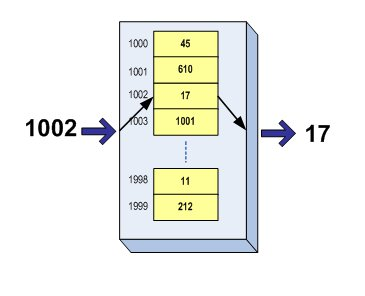
\includegraphics[scale=0.6]{images/adresse_memoire.jpg}
\caption{Exemple : on demande à notre mémoire de sélectionner la case
mémoire d'adresse 1002 et on récupère son contenu (ici, 17).}
\end{figure}

\begin{infobox}
  Plus généralement, toutes les mémoires disposent d'un mécanisme
  similaire pour retrouver les données.  Aussi, vous entendrez souvent
  le terme de \textbf{référence} qui désigne un moyen (comme une
  adresse) permettant de localiser une donnée. Il s'agit simplement
  d'une notion plus générale.
\end{infobox}

\subsection{Les variables}
\label{les-variables}

Tout cela est bien sympathique, mais manipuler explicitement des
références (des adresses si vous préférez) est un vrai calvaire, de
même que de s'évertuer à calculer en base deux. Heureusement pour
nous, les langages de programmation (et notamment le C), se chargent
d'effectuer les conversions pour nous et remplacent les références par
des variables.

Une variable correspondra à une portion de mémoire, appelée
\textbf{objet}, à laquelle nous donnerons un nom. Ce nom permettra
d'identifier notre variable, tout comme une référence permet
d'identifier une portion de mémoire parmi toutes les autres. Nous
allons ainsi pouvoir nommer les données que nous manipulons, chacun de
ces noms étant remplacés lors de la compilation par une référence (le
plus souvent une adresse).

\section{Déclarer une variable}
\label{declarer-une-variable}

Entrons maintenant dans le vif du sujet en apprenant à déclarer nos
variables. Tout d'abord, sachez qu'une variable est constituée de deux
éléments obligatoires :

\begin{itemize}
\item
  un \textbf{type} ;
\item
  un \textbf{identificateur} qui est en gros le « nom » de la variable.
\end{itemize}

Le type d'une variable permet d'indiquer ce qui y sera stocké, par
exemple : un caractère, un nombre entier, un nombre à virgule (ou
nombre \textbf{flottant}), etc. Pour préciser le type d'une variable,
il est nécessaire d'utiliser un mot-clé spécifique (il y en a donc un
pour chaque type).

Une fois que nous avons décidé du nom et du type de notre variable,
nous pouvons la créer (on dit aussi la déclarer) comme suit.

\begin{C}
type identificateur;
\end{C}

En clair, il suffit de placer un mot-clé indiquant le type de la
variable et de placer le nom qu'on lui a choisi immédiatement après.

\begin{attentionbox}
  Faites bien attention au point-virgule à la fin !
\end{attentionbox}

\subsection{Les types}
\label{les-types}

Comme dit précédemment, un type permet d'indiquer au compilateur quel
genre de données nous souhaitons stocker. Ce type va permettre de
préciser :

\begin{itemize}
\item
  toutes les valeurs que peut prendre la variable ;
\item les opérations qu'il est possible d'effectuer avec (il n'est par
  exemple pas possible de réaliser une division entière avec un nombre
  flottant, nous y reviendrons).
\end{itemize}

Définir le type d'une variable permet donc de préciser son contenu
potentiel et ce que nous pouvons faire avec. Le langage C fournit
sept\footnote{\footnotesize{Depuis la norme C99, un type entier
    supplémentaire a été ajouté : le type \mybox{long\ long\ int}. Ses
    bornes garanties par la norme sont comprises entre -9 223 372 036
    854 775 807 et 9 223 372 036 854 775 807 s'il est signé et entre 0
    et 18 446 744 073 709 551 615 s'il est non signé.}} types de base.

\begin{table}[ht!]
\centering
\rowcolors{1}{gris-clair-tab}{}
\begin{tabular}{|l|l|}\hline
\rowcolor{gris-tab-entete}\textbf{Type} & \textbf{Sert à stocker}\tabularnewline\hline
\textbf{char} & un caractère ou un entier\tabularnewline\hline
\textbf{short int} & un entier\tabularnewline\hline
\textbf{int} & un entier\tabularnewline\hline
\textbf{long int} & un entier\tabularnewline\hline
\textbf{float} & un flottant\tabularnewline\hline
\textbf{double} & un flottant\tabularnewline\hline
\textbf{long double} & un flottant\tabularnewline\hline
\end{tabular}
\caption{Les 7 types de base}
\end{table}

Les types \mybox{short\ int}, \mybox{int} et \mybox{long\ int} servent
tous à stocker des nombres entiers qui peuvent prendre des valeurs
positives, négatives, ou nulles. On dit qu'il s'agit de types signés
(car il peut comporter un signe). Pour ces trois types, il existe un
type équivalent dit \textbf{non signé}. Un type entier non signé est
un type entier qui n'accepte que des valeurs positives ou nulles : il
ne peut pas stocker de valeurs négatives. Pour déclarer des variables
d'un type non signé, il vous suffit de faire précéder le nom du type
entier du mot-clé \mybox{unsigned}.

Le type \mybox{char} peut lui aussi servir à stocker des nombres. Il
sert surtout au stockage de caractères, mais ces derniers étant
stockés dans l'ordinateur sous forme de nombres, il est possible de
stocker des nombres dans un \mybox{char}. Le seul problème, c'est que
ce type peut être signé ou non signé de base suivant les
compilateurs. Pour éviter les ennuis, spécifiez ce que vous souhaitez
lors de la déclaration : non signé (\mybox{unsigned\ char}) ou signé
(\mybox{signed\ char}).

{\begin{infobox} En cas de manque d'information concernant le type
    lors d'une déclaration, c'est le type \mybox{int} qui sera
    utilisé. Ainsi, \mybox{long} et \mybox{short} sont respectivement
    des raccourcis pour \mybox{long\ int} et \mybox{short\ int}. De
    même, le mot-clé \mybox{unsigned} seul signifie \mybox{unsigned\
      int}.
\end{infobox}

\subsubsection{Capacité d'un type}
\label{capacite-dun-type}

Tous les types stockant des nombres ont des bornes, c'est-à-dire une
limite aux valeurs qu'ils peuvent stocker. En effet, le nombre de
multiplets occupés par une variable est limité suivant son type. En
conséquence, il n'est pas possible de mettre tous les nombres
possibles dans une variable de type \mybox{int}, \mybox{float}, ou
\mybox{double}. Il y aura \emph{toujours} une valeur minimale et une
valeur maximale. Ces limites sont les suivantes.

\begin{table}[ht!]
\centering
\rowcolors{1}{gris-clair-tab}{}
\begin{tabular}{|l|l|l|}\hline
\rowcolor{gris-tab-entete}\textbf{Type} & \textbf{Minimum} & \textbf{Maximum}\tabularnewline\hline
\textbf{signed char} & -127 & 127\tabularnewline\hline
\textbf{unsigned char} & 0 & 255\tabularnewline\hline
\textbf{short} & -32 767 & 32 767\tabularnewline\hline
\textbf{unsigned short} & 0 & 65 535\tabularnewline\hline
\textbf{int} & -32 767 & 32 767\tabularnewline\hline
\textbf{unsigned int} & 0 & 65 535\tabularnewline\hline
\textbf{long} & -2 147 483 647 & 2 147 483 647\tabularnewline\hline
\textbf{unsigned long} & 0 & 4 294 967 295\tabularnewline\hline
\textbf{float} & -1 × 10\textsuperscript{37} & 1 × 10\textsuperscript{37}\tabularnewline\hline
\textbf{double} & -1 × 10\textsuperscript{37} & 1 × 10\textsuperscript{37}\tabularnewline\hline
\textbf{long double} & -1 × 10\textsuperscript{37} & 1 × 10\textsuperscript{37}\tabularnewline\hline
\end{tabular}
\caption{Les limites des types}
\end{table}

Si vous regardez bien ce tableau, vous remarquez que certains types ont
des bornes identiques. En vérité, les valeurs présentées ci-dessus sont
les minimums garantis par la norme\footnote{\footnotesize{Programming Language C,
  X3J11/88-090, § 2.2.4.2, Numerical limits}}

\subsubsection{Taille d'un type}
\label{taille-dun-type}

Peut-être vous êtes vous demandés pourquoi il existe autant de types
différents. La réponse est toute simple : la taille des mémoires était
très limitée à l'époque où le langage C a été créé. En effet, le
\href{https://upload.wikimedia.org/wikipedia/commons/c/c4/80_early_pcp_2.jpg}{PDP-11}
sur lequel le C a été conçu ne possédait que 24Ko de mémoire (pour
comparaison, une calculatrice TI-Nspire possède 100Mo de mémoire, soit
environ 4000 fois plus). Il fallait donc l'économiser au maximum en
choisissant le type le plus petit possible. Cette taille dépend des
machines, mais de manière générale, vous pouvez retenir les deux suites
d'inégalités suivantes : \mybox{char} ≤ \mybox{short} ≤ \mybox{int} ≤
\mybox{long} et \mybox{float} ≤ \mybox{double} ≤
\mybox{long\ double}.

Aujourd'hui ce n'est plus un problème, il n'est pas nécessaire de se
casser la tête sur quel type choisir (excepté si vous voulez programmer
pour de petits appareils où la mémoire est plus petite). En pratique,
nous utiliserons surtout \mybox{char} pour les caractères, \mybox{int}
ou \mybox{long} pour les entiers et \mybox{double} pour les flottants.

\subsection{Les identificateurs}
\label{les-identificateurs}

Maintenant que nous avons vu les types, parlons des identificateurs.
Comme dit précédemment, un identificateur est un nom donné à une
variable pour la différencier de toutes les autres. Et ce nom, c'est
au programmeur de le choisir. Cependant, il y a quelques limitations à
ce choix.

\begin{itemize}
\item seuls les 26 lettres de l'alphabet latin (majuscules ou
  minuscules), le trait de soulignement « \_ » (\emph{underscore} en
  anglais) et les chiffres sont acceptés. Pas d'accents, pas de
  ponctuation ni d'espaces ;
\item
  un identificateur ne peut pas commencer par un chiffre ;
\item
  les mots-clés ne peuvent pas servir à identifier une variable ; il
  s'agit de :
\end{itemize}

\begin{C}
auto     double  int       struct
break    else    long      switch
case     enum    register  typedef
char     extern  return    union
const    float   short     unsigned
continue for     signed    void
default  goto    sizeof    volatile
do       if      static    while
\end{C}

\begin{itemize}
\item deux variables ne peuvent avoir le même identificateur (le même
  nom).  Il y a parfois quelques exceptions, mais cela n'est pas pour
  tout de suite ;
\item
  les identificateurs peuvent être aussi longs que l'on désire,
  toutefois le compilateur ne tiendra compte que des 31 premiers
  caractères.
\end{itemize}

Voici quelques exemples pour bien comprendre.

\begin{table}[ht!]
\centering
\rowcolors{1}{gris-clair-tab}{}
\begin{tabular}{|l|l|l|}\hline
\rowcolor{gris-tab-entete}\textbf{Identificateur correct} & \textbf{Identificateur incorrect} & \textbf{Raison}\tabularnewline\hline
variable & Nom de variable & Espaces interdits\tabularnewline\hline
nombre\_de\_vie & 1nombre\_de\_vie & Commence par un chiffre\tabularnewline\hline
test & test! & Caractère « ! » interdit\tabularnewline\hline
un\_dernier\_pour\_la\_route1 & \mybox{continue} & Mot-clé réservé par le langage\tabularnewline\hline
\end{tabular}
\caption{Les identificateurs}
\end{table}

À noter que le C fait la différence entre les majuscules et les
minuscules (on dit qu'\textbf{il respecte la casse}). Ainsi les trois
identificateurs suivants sont différents.

\begin{C}
variable
Variable
VaRiAbLe
\end{C}

\subsection{Déclaration et initialisation}
\label{declaration-et-initialisation}

Maintenant que nous connaissons toutes les bases, entrainons-nous à
déclarer quelques variables.

\begin{C}
int main(void)
}
    double taille;
    unsigned int age;
    char caractere;
    short petite_valeur;

    return 0;
}
\end{C}

Il est possible de déclarer plusieurs variables \textbf{de même type}
sur une même ligne, en séparant leurs noms par une virgule.

\begin{C}
int age, taille, nombre;
\end{C}

Ceci permet de regrouper les déclarations suivant les rapports que les
variables ont entre elles.

\begin{C}
int annee, mois, jour;
int age, taille;
int x, y, z;
\end{C}

\subsubsection{Initialisation}
\label{initialisation}

En plus de déclarer une variable, il est possible de
\textbf{l'initialiser}, c'est-à-dire de lui attribuer une valeur. La
syntaxe est la suivante.

\begin{C}
type identificateur = valeur;
\end{C}

Ou comme ceci s'il s'agit d'un caractère.

\begin{C}
char identificateur = 'lettre';
\end{C}

Quelques exemples d'initialisations de variables.

\begin{C}
unsigned int age =25;
short petite_valeur =1;
const long abc =314159265;
char caractere = 'h';
\end{C}

\begin{infobox}
  Notez qu'une déclaration comporte le mot-clé \mybox{const}. Celui-ci
  permet de préciser qu'une variable ne pourra pas être modifiée par
  la suite. Ceci peut être utile pour stocker une valeur qui ne
  changera jamais (comme la constante \(\pi\) qui vaut toujours
  3,14159265).
\end{infobox}

\begin{attentionbox}
  Les déclarations doivent toujours se situer en début de bloc,
  c'est-à-dire juste après une accolade ouvrante.
\end{attentionbox}


\subsubsection{Initialisation des nombres flottants}
\label{initialisation-des-nombres-flottants}

\subsubsection*{En notation simple}

Petite précision concernant la manière d'initialiser une variable de
type flottant : celles-ci étant faites pour contenir des nombres à
virgule, à l'initialisation, il est nécessaire de placer cette «
virgule ». Toutefois, cette dernière est représentée par un point.

\begin{C}
const double pi = 3.14;
\end{C}

Ceci vient du fait que le C est une invention américaine et que les
anglophones utilisent le point à la place de la virgule.

Notez qu'il est important de bien placer ce point, \emph{même si vous
  voulez stocker un nombre entier}. Par exemple, vous ne devez pas
écrire \mybox{double a = 5} mais \mybox{double a = 5.} (certains
préfèrent \mybox{double a = 5.0}, cela revient au même). Si vous ne le
faites pas, vous risquez d'avoir quelques problèmes.

\subsubsection*{En notation scientifique}

Par ailleurs, sachez qu'il est également possible de représenter un
nombre flottant à l'aide de la notation scientifique, c'est-à-dire
sous la forme d'un nombre décimal et d'une puissance de dix. Cela se
traduit par un nombre flottant en notation simple (comme ci-dessus)
suivi de la lettre « e » ou « E » et d'un exposant \emph{entier}.

\begin{C}
double f = 1E-1; /* 1x10^-1 = 0.1 */
\end{C}

\subsection{Affectation}\label{affectation}

Nous savons donc déclarer (créer) nos variables et les initialiser
(leur donner une valeur à la création). Il ne nous reste plus qu'à
voir la dernière manipulation possible :
\textbf{l'affectation}. Celle-ci permet de modifier la valeur contenue
dans une variable pour la remplacer par une autre valeur.

Il va de soi que cette affectation n'est possible que pour les variables
qui ne sont pas déclarées avec le mot-clé \mybox{const} puisque, par
définition, de telles variables sont constantes et ne peuvent voir leur
contenu modifié.

Pour faire une affectation, il suffit d'opérer ainsi.

\begin{C}
identificateur = nouvelle_valeur;
\end{C}

Nous voyons que la syntaxe est similaire à celle d'une déclaration
avec initialisation. La seule différence, c'est que nous n'avons pas à
préciser le type. Celui-ci est en effet fixé une fois pour toute lors
de la déclaration de notre variable. Aussi, il n'est pas nécessaire de
le préciser à nouveau lors d'une affectation.

\begin{C}
age = 30;
taille = 177.5;
petite_valeur = 2
\end{C}

Notez qu'il n'y a aucune limite au nombre d'affectations, comme le
démontre l'exemple ci-dessous.

\begin{C}
petite_valeur = 2;
petite_valeur = 4;
petite_valeur = 8;
petite_valeur = 16;
petite_valeur = 8;
petite_valeur = 4;
petite_valeur = 2;
\end{C}

À chaque affectation, la variable va prendre une nouvelle valeur. Par
contre, ne mettez pas le type quand vous voulez changer la valeur,
sinon vous aurez le droit à une belle erreur du type «
\emph{redefinition of `nom\_de\_votre\_variable'} » car vous aurez
créé deux variables avec le même identificateur !

Le code suivant est donc incorrect.

\begin{C}
int age =15;
int age =20;
\end{C}

Si vous exécutez tous ces codes, vous verrez qu'ils n'affichent
toujours rien et c'est normal puisque nous n'avons pas demandé à notre
ordinateur d'afficher quoique ce soit. Nous apprendrons comment faire
au chapitre suivant.

\begin{erreurbox} Il n'y a pas de valeur par défaut en C.  Aussi, sans
  initialisation ou affectation, la valeur d'une variable est
  indéterminée ! Veillez donc à ce que vos variables aient une valeur
  connue avant de les utiliser !
\end{erreurbox}

\section{Les représentations octales et hexadécimales }

Pour terminer ce chapitre, nous vous proposons un petit aparté sur
deux représentations particulières : la représentation octale et la
représentation hexadécimale.

Nous avons déjà vu la représentation binaire au début de ce chapitre,
les représentations octale et hexadécimale obéissent au même schéma :
au lieu d'utiliser dix chiffres pour représenter un nombre, nous en
utilisons respectivement huit ou seize.

\begin{questionbox}
  Seize chiffres ?! Mais\ldots{} Je n'en connais que dix moi !
\end{questionbox}

La représentation hexadécimale est un peu déroutante de prime abord,
celle-ci ajoute six chiffres (en fait, six lettres) : a, b, c, d, e et
f. Pour vous aider, voici un tableau présentant les nombres de 1 à 16
en binaire, octal, décimal et hexadécimal.

\begin{table}[ht!]
\centering
\rowcolors{1}{gris-clair-tab}{}
\begin{tabular}{|l|l|l|l|}\hline
\rowcolor{gris-tab-entete}\textbf{Binaire} & \textbf{Octal} & \textbf{Décimal} & \textbf{Hexadécimal}\tabularnewline\hline
00001 & 1 & 1 & 1\tabularnewline\hline
00010 & 2 & 2 & 2\tabularnewline\hline
00011 & 3 & 3 & 3\tabularnewline\hline
00100 & 4 & 4 & 4\tabularnewline\hline
00101 & 5 & 5 & 5\tabularnewline\hline
00110 & 6 & 6 & 6\tabularnewline\hline
00111 & 7 & 7 & 7\tabularnewline\hline
01000 & 10 & 8 & 8\tabularnewline\hline
01100 & 14 & 12 & c\tabularnewline\hline
01101 & 15 & 13 & d\tabularnewline\hline
01110 & 16 & 14 & e\tabularnewline\hline
01111 & 17 & 15 & f\tabularnewline\hline
10000 & 20 & 16 & 10\tabularnewline\hline
\end{tabular}
\caption{Les nombres de 1 à 16 en binaire, octal, décimal et hexadécimal}
\end{table}

\begin{infobox}
  Notez que dix dans n'importe quelle base équivaut à cette base.
\end{infobox}

\begin{questionbox}
  Quel est l'intérêt de ces deux bases exactement ?
\end{questionbox}
  
L'avantage des représentations octale et hexadécimale est qu'il est
facilement possible de les convertir en binaire contrairement à la
représentation décimale. En effet, un chiffre en base huit ou en base
seize peut-être facilement traduit, respectivement, en trois ou quatre
\emph{bits}.

Prenons l'exemple du nombre 35 qui donne 43 en octal et 23 en
hexadécimal. Nous pouvons nous focaliser sur chaque chiffre un à un
pour obtenir la représentation binaire. Ainsi, du côté de la
représentation octale, 4 donne \mybox{100} et 3 \mybox{011}, ce qui
nous donne finalement \mybox{00100011}. De même, pour la
représentation hexadécimale, 2 nous donne \mybox{0010} et 3
\mybox{0011} et nous obtenons \mybox{00100011}. Il n'est pas possible
de faire pareil en décimal.

En résumé, les représentations octale et hexadécimale permettent de
représenter un nombre binaire de manière plus concise et plus lisible.

\section{Constantes octales et
hexadécimales}\label{constantes-octales-et-hexaduxe9cimales}

Il vous est possible de préciser la base d'une constante entière en
utilisant des préfixes. Ces préfixes sont \mybox{0} pour les
constantes octales et \mybox{0x} ou \mybox{0X} pour les constantes
hexadécimales.

\begin{C}
long a = 65535; /* En décimal */
int b =0777; /* En octal */
short c = 0xFF; /* En hexadécimal */
\end{C}

\begin{infobox}
  Les lettres utilisées pour la représentation hexadécimale peuvent
  être aussi bien écrites en minuscule qu'en majuscule.
\end{infobox}


\begin{questionbox}
  Il n'est pas possible d'utiliser une constante en base deux ?
\end{questionbox}

Malheureusement, non, le langage C ne permet pas d'utiliser de telles
constantes.

\hrulefill
    
Voilà, c'est la fin de ce chapitre. Nous avons vu beaucoup de choses,
n'hésitez pas à potasser pour bien assimiler tout ça. Les variables
sont vraiment la base de la programmation, aussi il nécessaire de bien
les comprendre. Rendez-vous au prochain chapitre qui sera très
intéressant : vous pourrez par exemple demander l'âge de l'utilisateur
pour ensuite l'afficher !
\chapter{Manipulations basiques des entrées/sorties}

Durant l'exécutiond'un programme, le processeur a besoin de communiquer 
avec le reste du matériel. Ces échanges d'informations sont les \textbf{entrées} et les
\textbf{sorties} (ou \emph{input} et \emph{output} pour les
anglophones), souvent abrégées E/S (ou I/O par les anglophones).

Les entrées permettent de recevoir une donnée en provenance de certains
périphériques. Les données fournies par ces entrées peuvent être une
information envoyée par le disque dur, la carte réseau, le clavier, la
souris, un CD, un écran tactile, bref par n'importe quel périphérique.
Par exemple, notre clavier va transmettre des informations sur les
touches enfoncées au processeur : notre clavier est donc une entrée.

À l'inverse, les sorties vont transmettre des données vers ces
périphériques. On pourrait citer l'exemple de l'écran : notre ordinateur
lui envoie des informations pour qu'elles soient affichées.

Dans ce chapitre, nous allons apprendre différentes fonctions fournies
par le langage C qui vont nous permettre d'envoyer des informations vers
nos sorties et d'en recevoir depuis nos entrées. Vous saurez ainsi
comment demander à un utilisateur de fournir une information au clavier
et comment afficher quelque chose sur la console.

\section{Les sorties}

Intéressons-nous dans un premier temps aux sorties. Afin
d'afficher du texte, nous avons besoin d'une \textbf{fonction}.

Une fonction est un morceau de code qui a un but, une \emph{fonction}
particulière et qui peut être \textbf{appelée} à l'aide d'une référence,
le plus souvent le nom de cette fonction (comme pour une variable,
finalement). En l'occurrence, nous allons utiliser une fonction qui a
pour objectif d'afficher du texte dans la console : la fonction
\mybox{printf()}.

\subsection{Première approche}
\label{premiere-approche}

Un exemple valant mieux qu'un long discours, voici un premier exemple.


\begin{C}
#include<stdio.h>}

int main(void)
{
     printf("Bonjour tout le monde !\n");
    return 0;
}
\end{C}


\begin{C}
Bonjour tout le monde !
\end{C}

Deux remarques au sujet de ce code.


\begin{C}
#include<stdio.h>
\end{C}


Il s'agit d'une \textbf{directive du préprocesseur}, facilement
reconnaissable car elles commencent toutes par le symbole \mybox{\#}.
Celle-ci sert à inclure un fichier (« stdio.h ») qui contient les
références de différentes fonctions d'entrée et sortie (« \emph{stdio} »
est une abbréviation pour « \emph{\textbf{St}andar\textbf{d i}nput
\textbf{o}utput} », soit « Entrée-sortie standard »).

Un fichier se terminant par l'extension « .h » est appelé un
\textbf{fichier d'en-tête} (\emph{header} en anglais) et fait partie
avec d'autre d'un ensemble plus large appelée la \textbf{bibliothèque
standard} (« standard » car elle est prévue par la
norme{\footnote{\footnotesize{Programming Language C, X3J11/88-090, §
4, Library.}}.


\begin{C}
 printf("Bonjour tout le monde !\n");
\end{C}


Ici, nous \textbf{appelons} la fonction \mybox{printf()} (un appel de
fonction est toujours suivi d'un groupe de parenthèses) avec comme
\textbf{argument} (ce qu'il y a entre les parenthèses de l'appel) un
texte (il s'agit plus précisément d'une \textbf{chaîne de caractères},
qui est toujours comprise entre deux guillemets double). Le
\mybox{\textbackslash n} est un caractère spécial qui représente un
retour à la ligne, cela est plus commode pour l'affichage.

Le reste devrait vous être familier.

\subsection{Les formats}
\label{les-formats}

Bien, nous savons maintenant afficher une phrase, mais ce serait quand
même mieux de pouvoir voir les valeurs de nos variables. Comment faire ?
\emph{Hé} bien, pour y parvenir, la fonction \mybox{printf()} met à
notre disposition des \textbf{formats}. Ceux-ci sont en fait des sortes
de repères au sein d'un texte qui indique à \mybox{printf()} que la
valeur d'une variable est attendue à cet endroit. Voici un exemple pour
une variable de type \mybox{int}.


\begin{C}
#include<stdio.h>}

int main(void)
{
    int variable = 20 ;

    printf("%d\n", variable);
    return 0 ;
}
\end{C}


\begin{C}
20
\end{C}

Nous pouvons voir que le texte de l'exemple précédent a été remplacé par
\mybox{\%d}, seul le \mybox{\textbackslash n} a été conservé. Un
format commence toujours par le symbole \mybox{\%} et est suivi par une
ou plusieurs lettres qui indiquent le type de données que nous
souhaitons voir afficher. Cette suite de lettre est appelée un
\textbf{indicateur de conversion}. En voici une liste non
exhaustive\footnote{\footnotesize{Pour le type \mybox{long long}
introduit en C99, les indicateurs de conversions sont \mybox{lld} et
\mybox{llu}. Il en va de même pour \mybox{scanf()}.}}

\clearpage

\begin{table}[ht!]
\centering
\rowcolors{1}{}{gris-clair-tab}
\begin{tabular}{|l|l|}\hline
\rowcolor{gris-tab-entete}\textbf{Type} & \textbf{Indicateur(s) de conversion}\tabularnewline\hline
\textbf{char} & c, d (ou i)\tabularnewline\hline
\textbf{short} & d (ou i)\tabularnewline\hline
\textbf{int} & d (ou i)\tabularnewline\hline
\textbf{long} & ld (ou li)\tabularnewline\hline
\textbf{unsigned char} & u, x (ou X) ou o\tabularnewline\hline
\textbf{unsigned short} & u, x (ou X) ou o\tabularnewline\hline
\textbf{unsigned int} & u, x (ou X) ou o\tabularnewline\hline
\textbf{unsigned long} & lu, lx (ou lX) ou lo\tabularnewline\hline
\textbf{float} & f, e (ou E) ou g (ou G)\tabularnewline\hline
\textbf{double} & f, e (ou E) ou g (ou G)\tabularnewline\hline
\textbf{long double} & Lf, Le (ou LE) ou Lg (ou LG)\tabularnewline\hline
\end{tabular}
\caption{Liste des indicateurs de conversion}
\end{table}


\begin{infobox}
Notez que pour le type \mybox{char},
l'indicateur est soit \mybox{c}, soit \mybox{d} (ou \mybox{i}). Cela
dépend si vous l'utilisez pour contenir un caractère ou un entier.
Également, notez que les indicateurs de conversions sont identiques pour
les types \mybox{char} (s'il stocke un entier), \mybox{short} et
\mybox{int} (pareil pour leurs équivalents non signés) ainsi que pour
les types \mybox{float} et \mybox{double}.
\end{infobox}

Les indicateurs \mybox{x}, \mybox{X} et \mybox{o} permettent
d'afficher un nombre en représentation hexadécimale ou octale
(l'indicateur \mybox{x} affiche les lettres en minuscules alors que
l'indicateur \mybox{X} les affiches en majuscules).

Les indicateurs \mybox{f}, \mybox{e} et \mybox{g} permettent quant à
eux d'afficher un nombre flottant. L'indicateur \mybox{f} affiche un
nombre en notation simple avec, par défaut, six décimales ; l'indicateur
\mybox{e} affiche un nombre flottant en notation scientifique
(l'indicateur \mybox{e} utilise la lettre « e » avant l'exposant alors
que l'indicateur « E » emploie la lettre « E ») et l'indicateur
\mybox{g} choisi quant à lui entre les deux notations précédentes
suivant le nombre fourni et supprime la partie fractionnaire si elle est
nulle de sorte que l'écriture soit concise (la différence entre les
indicateurs \mybox{g} et \mybox{G} est identique à celle entre les
indicateurs \mybox{e} et \mybox{E}).

Allez, un petit exemple pour reprendre tout cela et retravailler le
chapitre précédent par la même occasion.


\begin{C}
#include<stdio.h>}

int main(void )
{
    char z = 'z';
    char a = 10;
    unsigned} short b = 20;
    int c = 30;
    long d = 40;
    float e = 50 .;
    double f = 60.0;
    long double g = 70.0;

     printf("%c\n", z);
     printf("%d\n", a);
     printf("%u\n", b);
     printf("%o\n", b);
     printf("%x\n", b);
     printf("%d\n", c);
     printf("%li\n", d);
     printf("%f\n", e);
     printf( "%e\n", f);
     g = 80.0;
     printf( "%Lg\n", g);
    return 0;
}
\end{C}


\begin{C}
z
10
20
24
14
30
40
50.000000
6.000000e+01
80
\end{C}

\begin{infobox}
Si vous souhaitez afficher le caractère \mybox{\%} vous devez le doubler : \mybox{\%\%}.
\end{infobox}

\subsection{Précision des nombres flottants}\label{precision-des-nombres-flottants}

Vous avez peut-être remarquer que lorsqu'un flottant est affiché avec le
format \mybox{f}, il y a un certain nombre de zéros qui suivent (par
défaut six) et ce, peu importe qu'ils soient utiles ou non. Afin d'en
supprimer certains, vous pouvez spécifier une \textbf{précision}.
Celle-ci correspond au nombre de chiffre suivant la virgule qui seront
affichés. Elle prend la forme d'un point suivi par un nombre : la
quantité de chiffres qu'il y aura derrière la virgule.


\begin{C}
double x = 42.42734;

printf("%.2f", x);
\end{C}


\begin{C}
42.43
\end{C}

\subsection{Les caractères spéciaux}\label{les-caracteres-speciaux}

Dans certains cas, nous souhaitons obtenir un résultat à l'affichage
(saut de ligne, une tabulation, un retour chariot, etc.). Cependant, ils
ne sont pas particulièrement pratiques à insérer dans une chaîne de
caractères. Aussi, le C nous permet de le faire en utilisant une
\textbf{séquence d'échappement}. Il s'agit en fait d'une suite de
caractères commençant par le symbole \mybox{\textbackslash} et suivie
d'une lettre. En voici une liste non exhaustive.

\begin{table}[ht!]
\centering
\begin{tabular}{|l|l|}\hline
\rowcolor{gris-tab-entete}\textbf{Séquence d'échappement} & \textbf{Signification}\tabularnewline\hline
\rowcolor{gris-clair-tab} \mybox{\textbackslash}& Caractère d'appel\tabularnewline\hline
\mybox{\textbackslash b} & Espacement arrière\tabularnewline\hline
\rowcolor{gris-clair-tab} \mybox{\textbackslash f} & Saut de page\tabularnewline\hline
\mybox{\textbackslash n} & Saut de ligne\tabularnewline\hline
\rowcolor{gris-clair-tab} \mybox{\textbackslash r} & Retour chariot\tabularnewline\hline
\mybox{\textbackslash t} & Tabulation horizontale\tabularnewline\hline
\rowcolor{gris-clair-tab} \mybox{\textbackslash v} & Tabulation verticale\tabularnewline\hline
\mybox{\textbackslash "} & Le symbole « \mybox{"} »\tabularnewline\hline
\rowcolor{gris-clair-tab} \mybox{\textbackslash \textbackslash} & Le symbole « \mybox{\textbackslash} » lui-même\tabularnewline\hline
\end{tabular}
\caption{Les nombres de 1 à 16 en binaire, octal, décimal et hexadécimal.}
\end{table}

En général, vous n'utiliserez que le saut de ligne, la tabulation
horizontale et de temps à autre le retour chariot, les autres n'ont
quasiment plus d'intérêt. Un petit exemple pour illustrer leurs effets.


\begin{C}
#include<stdio.h>

int main(void)
{
     printf( "Quelques sauts de ligne\n\n\n");
     printf( " \tIl y a une tabulation avant moi !\n");
     printf( "Je voulais dire que... \r ");
     printf( "Hey ! Vous pourriez me laisser parler !\n");
    return 0 ;
}
\end{C}


\begin{C}
Quelques sauts de ligne


        Il y a une tabulation avant moi !
Hey ! Vous pourriez me laisser parler !
\end{C}

\begin{infobox}
Le retour chariot provoque un retour
au début de la ligne courante. Ainsi, il est possible d'écrire
par-dessus un texte affiché.
\end{infobox}

\subsection{Sur plusieurs lignes}\label{sur-plusieurs-lignes}

Notez qu'il est possible d'écrire un long texte sans appeler plusieurs
fois la fonction \mybox{printf()}. Pour ce faire, il suffit de le
diviser en plusieurs chaînes de caractères.


\begin{C}
#include<stdio.h>

int main(void )
{
     printf("Texte écrit sur plusieurs "
	    "lignes dans le code source "
	    "mais sur une seule dans la console.\n");
    return 0;
}
\end{C}


\begin{C}
Texte écrit sur plusieurs lignes dans le code source mais sur une seule dans la console.
\end{C}

\section{Interagir avec l'utilisateur }
Maintenant que nous savons déclarer, utiliser et même
afficher des variables, nous sommes fin prêts pour interagir avec
l'utilisateur.
En effet, jusqu'à maintenant, nous nous sommes contentés
d'afficher des informations. Nous allons à présent voir comment en
récupérer grâce à la fonction \mybox{scanf()}, dont l'utilisation est
assez semblable à \mybox{printf()}.


\begin{C}
#include<stdio.h>

int main(void)
{
    int age;

     printf("Quel âge avez-vous ? ");
     scanf("%d", &age);
     printf("Vous avez %d an(s)\n ", age);
    return 0 ;
}
\end{C}


\begin{C}
Quel age avez-vous ? 15
Vous avez 15 an(s).
\end{C}

Comme vous le voyez, l'appel à \mybox{scanf()} ressemble très fort à
celui de \mybox{printf()} mise à part l'absence du caractère spécial\mybox{\textbackslash n} (qui n'a pas d'intérêt puisque nous
récupérons des informations) et le symbole \mybox{\&}.

À son sujet, souvenez-vous de la brève explication sur la mémoire au
début du chapitre précédent. Celle-ci fonctionne comme une armoire avec
des tiroirs (les adresses mémoires) et des objets dans ces tiroirs (nos
variables). La fonction \mybox{scanf()} a besoin de connaitre
l'emplacement en mémoire de nos variables afin de les modifier. Afin
d'effectuer cette opération, nous utilisons le symbole \mybox{\&} (qui
est en fait un opérateur que nous verrons en détail plus tard). Ce
concept de transmission d'adresses mémoires est un petit peu difficile à
comprendre au début, mais ne vous inquiétez pas, vous aurez l'occasion
de bien revoir tout cela en profondeur dans le chapitre traîtant des
pointeurs.

Ici, \mybox{scanf()} attend patiemment que l'utilisateur saisisse un
nombre au clavier afin de modifier la valeur de la variable \emph{age}.
On dit que c'est une \textbf{fonction bloquante}, car elle suspend
l'exécution du programme tant que l'utilisateur n'a rien entré.

Pour ce qui est des indicateurs de conversions, ils sont un peu
différents de ceux de \mybox{printf()}.

\begin{table}[ht!]
\centering
\begin{tabular}{|l|l|}\hline
\rowcolor{gris-tab-entete}\textbf{Type} & \textbf{Indicateur(s) de conversion}\tabularnewline\hline
\rowcolor{gris-clair-tab}\textbf{char} & c\tabularnewline\hline
\textbf{short} & hd ou hi\tabularnewline\hline
\rowcolor{gris-clair-tab}\textbf{int} & d ou i\tabularnewline\hline
\textbf{long} & ld ou li\tabularnewline\hline
\rowcolor{gris-clair-tab}\textbf{unsigned short} & hu, hx ou ho\tabularnewline\hline
\textbf{unsigned int} & u, x ou o\tabularnewline\hline
\rowcolor{gris-clair-tab}\textbf{unsigned long} & lu, lx ou lo\tabularnewline\hline
\textbf{float} & f\tabularnewline\hline
\rowcolor{gris-clair-tab}\textbf{double} & lf\tabularnewline\hline
\textbf{long double} & Lf\tabularnewline\hline
\end{tabular}
\end{table}

\begin{erreurbox}
Faites bien attention aux différences ! Si
vous utilisez le mauvais format, le résultat ne sera pas celui que vous
attendez. Les changements concernent les types \mybox{char},
\mybox{short} et \mybox{double}.
\end{erreurbox}

\begin{infobox}
Notez que l'indicateur \mybox{c} ne
peut être employé que pour récupérer un caractère et non un nombre.
\end{infobox}

\begin{infobox}
Remarquez également qu'il n'y a plus
qu'un seul indicateur pour récupérer un nombre hexadécimal : \mybox{x}
(l'utilisation de lettres majuscules ou minuscules n'a pas
d'importance).
\end{infobox}

En passant, sachez qu'il est possible de lire plusieurs entrées en même
temps, par exemple comme ceci.


\begin{C}
int x, y;

 scanf("%d %d" , &x, &y);
 printf("x = %d | y = %d \n" , x, y);
\end{C}


L'utilisateur a deux possibilités, soit insérer un (ou plusieurs)
espace(s) entre les valeurs, soit insérer un (ou plusieurs) retour(s) à
la ligne entre les valeurs.

\begin{C}
14
6
x = 14 | y = 6
\end{C}

\begin{C}
14 6
x = 14 | y = 6
\end{C}

La fonction \mybox{scanf()} est en apparence simple (oui, \emph{en
apparence}), mais son utilisation peut devenir très complexe lorsqu'il
est nécessaire de vérifier les entrées de l'utilisateur (entre autres).
Cependant, à votre niveau, vous ne pouvez pas encore effectuer de telles
vérifications. Ce n'est toutefois pas très grave, nous verrons cela en
temps voulu.;)

\hrulefill

Maintenant, vous êtes capable de communiquer avec l'utilisateur.
Cependant, nos actions sont encore un peu limitées. Nous verrons dans
les prochains chapitres comment mieux interagir avec
l'utilisateur.
\chapter{Les opérations mathématiques}

Nous savons désormais déclarer,
affecter et initialiser une variable, mais que diriez-vous d'apprendre à
réaliser des opérations dessus ? Il est en effet possible de réaliser
des calculs sur nos variables, comme les additionner, les diviser voire
même des opérations plus complexes. C'est le but de cette sous-partie.
Nous allons donc enfin transformer notre ordinateur en grosse calculette
programmable !

\section{Les opérations mathématiques de base}

Jusqu'à présent, nous nous sommes contenté d'afficher
  du texte et de manipuler très légèrement les variables. Voyons à
  présent comment nous pouvons réaliser quelques opérations de base. Le
  langage C nous permets d'en réaliser cinq :}.
  
  \begin{itemize}
\item
  l'addition (opérateur \mybox{+}) ;
\item
  la soustraction (opérateur \mybox{-}) ;
\item
  la multiplication (opérateur \mybox{*}) ;
\item
  la division (opérateur \mybox{/}) ;
\item
  le modulo (opérateur \mybox{\%}).
\end{itemize}

\begin{infobox}
Le langage C fournit bien entendu
d'autres fonctions mathématiques et d'autres opérateurs, mais il est
encore trop tôt pour vous les présenter.
\end{infobox}


\section{Division et modulo}
\label{division-et-modulo}

Les quatre premières opérations vous sont connues depuis l'école
primaire. Cependant, une chose importante doit être précisée concernant
la division : quand les deux nombres manipulés sont des entiers, il
s'agit d'une division entière. Autrement dit, le quotient sera un entier
et il peut y avoir un reste. Par exemple, 15 ÷ 6, ne donnera pas 2,5
(division réelle), mais un quotient de 2, avec un reste de 3.

\begin{C}
printf("15 / 6 = %d\n", 15 / 6);
\end{C}

\begin{C}
15 / 6 = 2
\end{C}

Le modulo est un peu le complément de la division entière : au lieu de
donner le quotient, il renvoie le reste d'une division euclidienne. Par
exemple, le modulo de 15 par 6 est 3, car 15 = 2 × 6 + 3.

\begin{C}
printf("15 % 6 = %d\n", 15 % 6);
\end{C}

\begin{C}
15 % 6 = 3
\end{C}

Avec des flottants, la division se comporte autrement et n'est pas une
division avec reste. La division de deux flottants donnera un résultat «
exact », avec potentiellement plusieurs chiffres après la virgule.

\begin{C}
printf("15 / 6 = %f\n", 15. / 6.);   /* En C, ce n’est pas la même chose que 15 / 6 */
\end{C}

\begin{C}
15 / 6 = 2.500000
\end{C}

\section{Utilisation}
\label{utilisation}

Il est possible d'affecter le résultat d'une expression contenant des
calculs à une variable, comme lorsque nous les utilisons comme argument
de \mybox{printf()}.

\begin{C}
#include <stdio.h>

int main(void)
{
    int somme = 5 + 3;

    printf("5 + 3 = %d\n", somme);
    return 0;
}
\end{C}

\begin{C}
5 + 3 = 8
\end{C}

Toute opération peut manipuler :

\begin{itemize}
\item
  des constantes ;
\item
  des variables ;
\item
  les deux à la fois.
\end{itemize}

Voici un exemple avec des constantes.

\begin{C}
#include <stdio.h>

int main(void)
{
    printf("2 + 3 = %d\n", 2 + 3);
    printf("8 - 12 = %d\n", 8 - 12);
    printf("6 x 7 = %d\n", 6 * 7);
    printf("11 % 4 = %d\n", 11 % 4);
    return 0;
}
\end{C}

\begin{C}
2 + 3 = 5
8 - 12 = -4
6 x 7 = 42
11 % 4 = 3
\end{C}

Un autre avec des variables.

\begin{C}
int a = 5;
int b = 3;
int somme = a + b;

printf("%d + %d = %d\n", a, b, somme);
\end{C}

\begin{C}
5 + 3 = 8
\end{C}

Et enfin, un exemple qui mélange variables et constantes.

\begin{C}
int a = 5;
int b = 65;

printf("%d\n", b / a * 2 + 7 % 2);
\end{C}

\begin{C}
27
\end{C}

\section{La priorité des opérateurs}
\label{la-priorite-des-operateurs}

Dans l'exemple précédent, nous avons utilisé plusieurs opérations dans
une même ligne de code, une même expression. Dans ces cas là, faites
attention à la \textbf{priorité des opérateurs} ! Comme en
mathématiques, certains opérateurs passent avant d'autres : les
opérateurs \mybox{* \textbackslash \%} ont une priorité supérieure par rapport aux
opérateurs \mybox{+ -}.

Dans le code ci-dessous, c'est \mybox{c * 4} qui sera exécuté
d'abord, puis \mybox{b} sera ajouté au résultat. Faites donc attention
sous peine d'avoir de mauvaises surprises. Dans le doute, ajoutez des
parenthèses.

\begin{C}
c a = b + c * 4;}
\end{C}

\section{Les expressions}

Il est possible de combiner opérateur, variables et constantes pour
former des \textbf{expressions}, des lignes de code qui sont évaluées et
produisent un résultat. Les lignes de code suivantes sont toutes des
expressions.

\begin{C}
"Bonjour !"
2 + 3
10 > 2
\end{C}

Généralement, une expression ne peut être écrite seule et doit faire
partie d'une \textbf{instruction}. La frontière entre instruction et
expression est assez floue puisqu'une instruction peut être composée de
nombreuses expressions. Le code ci-dessous est un exemple d'instruction
qui est \emph{quasi} une expression (on parle
d'\textbf{expression-instruction}).

\begin{C}
x = 2 + 3;
\end{C}

Nous donnons en effet un ordre à l'ordinateur (« affecte la valeur 2 + 3
à \mybox{x} »), mais c'est aussi une expression qui produit la valeur 5
comme résultat. Vous verrez qu'en C, la majorité des lignes de code sont
des instructions-expressions. C'est ce qui est appellé la
\textbf{programmation impérative}. C'est le choix des concepteurs du
langage, mais ce n'est pas la seule possibilité (il en existe d'autres,
mais ça ne nous concerne pas en tant qu'utilisateurs du C).

\section{Type d'une expression}
\label{type-dune-expression}

Vous avez sans doute remarqué que nous avons utilisé directement des
expressions (\mybox{2 + 3} par exemple) comme argument de la fonction
\mybox{printf()}. Rien de bien surprenant me direz-vous\ldots{} À un
détail près : quel indicateur de format doit-on utiliser ? Autrement
dit, quel est le type d'une expression ? D'ailleurs, ont-elles un type ?

\emph{Hé} bien, oui. Tout comme les variables, les expressions ont un
type. Ce dernier dépend toutefois du type des éléments qui la compose.
En l'occurrence, une constante entière comme \mybox{2} ou \mybox{3}
est par défaut de type \mybox{int}. Le résultat d'une somme, par
exemple, sera donc également de type \mybox{int}. Les constantes
flottantes comme \mybox{5.} ou \mybox{78.0} sont, elles, de type
\mybox{double} et le résultat d'une opération sera alors de type
\mybox{double}.

\begin{questionbox}
D'accord, mais si j'additionne un
\mybox{int} avec un \mybox{double}, cela me donne quoi ?
\end{questionbox}

Heureusement pour nous, la norme\footnote{Programming Language C,
  X3J11/88-090, § 3.2.1.5, Usual arithmetic conversions.} a prévu ces
différents cas et a fixé des règles :

\begin{itemize}
\item
  si un opérande est de type \mybox{long double}, le résultat est de
  type \mybox{long double} ; si non
\item
  si un opérande est de type \mybox{double}, le résultat est de type
  \mybox{double} ; si non
\item
  si un opérande est de type \mybox{float}, le résultat est de type
  \mybox{float} ; si non
\item
  si un opérande est de type \mybox{unsigned long}, le résultat est de
  type \mybox{unsigned long}; si non
\item
  si un opérande est de type \mybox{long}, le résultat est de type
  \mybox{long}; si non
\item
  si un opérande est de type \mybox{unsigned int}, le résultat est de
  type \mybox{unsigned int}; si non
\item
  le résultat est de type \mybox{int}.
\end{itemize}

\subsection{Suffixes}
\label{suffixes}

\begin{questionbox}
\emph{Heu}\ldots{} D'accord, mais vous
venez de dire que les constantes entières étaient de type \mybox{int}
et que les constantes flottantes étaient de type \mybox{double}. Du
coup, je fais comment pour obtenir une constante d'un autre type ?
\end{questionbox}

À l'aide d'un suffixe. Celui-ci se place à la fin de la constante et
permet de modifier son type. En voici la liste complète\footnote{\footnotesize{Pour le
  type \mybox{long long} introduit en C99, le suffixe est \mybox{LL}
  ou \mybox{ll}}}.


\begin{table}[ht!]
\centering
 \begin{tabular}{|l|l|}\hline
\rowcolor{gris-tab-entete}\textbf{Type} & \textbf{Suffixe}\tabularnewline\hline
\rowcolor{gris-clair-tab}u ou U & \textbf{unsigned}\tabularnewline\hline
l ou L & \textbf{long}\tabularnewline\hline
\rowcolor{gris-clair-tab}f ou F & \textbf{float}\tabularnewline\hline
l ou L & \textbf{long double}\tabularnewline\hline
 \end{tabular}
\end{table}

\begin{infobox}
Notez que les suffixes \mybox{L} (ou \mybox{l}) et \mybox{U} (ou \mybox{u}) peuvent être combinés.
\end{infobox}

  
\subsection{Exemple}
\label{exemple}

Allez, un petit récapitulatif.

\begin{C}
#include <stdio.h>


int main(void)
{
    /* long double + int = long double */
    printf("78.56 + 5 = %Lf\n", 78.56L + 5);

    /* long + double = double */
    printf("5678 + 2.2 = %f\n", 5678L + 2.2);

    /* long + unsigned long = unsigned long */
    printf("2 + 5 = %lu\n", 2L + 5UL);

    /* long + int = long */
    printf("1 + 1 = %ld\n", 1L + 1);
    return 0;
}
\end{C}

\begin{C}
78.56 + 5 = 83.560000
5678 + 2.2 = 5680.200000
2 + 5 = 7
1 + 1 = 2
\end{C}

\begin{infobox}
Nous vous conseillons d'opter pour
les lettres majuscules qui ont l'avantage d'être plus lisibles.
\end{infobox}

\section{Conversions de types}
\label{conversions-de-types}

La \textbf{conversion de type} est une opération qui consiste à changer
le type de la valeur d'une expression. Ainsi, il vous est par exemple
possible de convertir une valeur de type \mybox{float} en type
\mybox{int}.

\subsection{Perte d'informations}
\label{perte-dinformations}

Une perte d'informations survient quand le type d'une variable est
converti vers un autre type ayant une capacité plus faible \emph{et} que
celui-ci ne peut pas contenir la valeur d'origine. Si, par exemple, nous
convertissons un \mybox{double} de cent chiffres en un \mybox{int}, il
y a perte d'informations, car le type \mybox{int} ne peut pas contenir
un nombre de cent chiffres. Retenez donc bien cette assertion : une
conversion d'un type \(T\) vers un type \(S\) de plus faible capacité
entraîne une perte d'informations (une perte de précision pour les
nombres).

Les conversions peuvent être vicieuses et doivent être manipulées avec
précaution, au risque de tomber sur des valeurs fausses en cas de perte
d'informations. Nous découvrirons d'ici quelques chapitres comment
connaître la taille d'un type pour éviter ces pertes d'informations.

\subsection{Deux types de conversions}
\label{deux-types-de-conversions}

Il existe deux types de conversions : les conversions explicites et les
conversions implicites.

\subsubsection*{Les conversions explicites}
\label{les-conversions-explicites}

Les \textbf{conversions explicites} sont des conversions demandées par
le programmeur. Elles s'utilisent suivant ce modèle.

\begin{C}
(<Type>)<Expression>
\end{C}

Voici par exemple un code où nous demandons explicitement la conversion
d'un \mybox{double} en \mybox{int}.

\begin{C}
int a;
const double pi = 3.14;

a = (int)pi;
\end{C}

La valeur de \mybox{pi} reste inchangée, elle vaudra toujours 3.14 dans
la suite du programme. Par contre, \mybox{a} vaut maintenant 3, puisque
la valeur de \mybox{pi} a été convertie en \mybox{int}.

\subsubsection*{Conversions implicites}
\label{conversions-implicites}

Les \textbf{conversions implicites} sont des conversions spécifiées par
la norme et réalisées automatiquement par le compilateur. En général,
cela ne pose pas de problèmes et cela est même désirable. Par exemple,
il y a toujours une conversion implicite dans le cadre d'une
affectation.

Ainsi, la conversion explicite du code précédent n'est en fait pas
nécessaire.

\begin{C}
int a;
const double pi = 3.14;

/* Il y a conversion implicite du type double vers le type int. */
a = pi;
\end{C}

\section{Sucre syntaxique }
\label{sucre-syntaxique}

Dans les expressions vues au-dessus, nous avons utilisé des affectations pour
sauvegarder le résultat de l'opération dans une variable. Les
expressions obtenues ainsi sont assez longues et on peut se demander
s'il existe des moyens pour écrire moins de code. \emph{Hé} bien, le
langage C fournit des écritures pour se simplifier la vie. Certains cas
particuliers peuvent s'écrire avec des raccourcis, du « \textbf{sucre
syntaxique} ».

\section{Les opérateurs combinés}
\label{les-operateurs-combines}

Comment vous y prendriez-vous pour multiplier une variable par trois ?
La solution qui devrait vous venir à l'esprit serait d'affecter à la
variable son ancienne valeur multipliée par trois.

\begin{C}
int variable = 3;

variable = variable * 3;
printf("variable * 3 = %d\n", variable);
\end{C}

\begin{C}
variable * 3 = 9
\end{C}

Ce qui est parfaitement correct. Cependant, cela implique de devoir
écrire deux fois le nom de la variable, ce qui est quelques peu pénible
et source d'erreurs. Aussi, il existe des opérateurs combinés qui
réalisent une affectation et une opération en même temps.

\begin{table}[ht!]
\centering
 \begin{tabular}{|l|l|}\hline
\rowcolor{gris-tab-entete}\textbf{Opérateur combiné} & \textbf{Équivalent à}\tabularnewline\hline
variable += nombre & variable = variable + nombre\tabularnewline\hline
\rowcolor{gris-clair-tab}variable -= nombre & variable = variable - nombre\tabularnewline\hline
variable *= nombre & variable = variable * nombre\tabularnewline\hline
\rowcolor{gris-clair-tab}variable /= nombre & variable = variable / nombre\tabularnewline\hline
variable \%= nombre & variable = variable \% nombre\tabularnewline\hline
 \end{tabular}
\end{table}


Avec le code précédent, nous obtenons ceci.

\begin{C}
int variable = 3;

variable *= 3;
printf("variable * 3 = %d\n", variable);
\end{C}

\begin{C}
variable * 3 = 9
\end{C}

\subsection{L'incrémentation et la décrémentation}
\label{lincrementation-et-la-decrementation}

L'\textbf{incrémentation} et la \textbf{décrémentation} sont deux
opérations qui, respectivement, ajoute ou enlève une unité à une
variable. Avec les opérateurs vu précédemment, cela se traduit par le
code ci-dessous.

\begin{C}
variable += 1; /* Incrémentation */
variable -= 1; /* Décrémentation */
\end{C}

Cependant, ces deux opérations étant très souvent utilisées, aussi elles
ont droit chacune à un opérateur spécifique disponible sous deux formes
:

\begin{itemize}
\item
  une forme \textbf{préfixée} ;
\item
  une forme \textbf{suffixée}.
\end{itemize}

La forme préfixée s'écrit comme ceci.

\begin{C}
++variable; /* Incrémentation */
--variable; /* Décrémentation */
\end{C}

La forme suffixée s'écrit comme cela.

\begin{C}
variable++; /* Incrémentation */
variable--; /* Décrémentation */
\end{C}

Le résultat des deux paires d'opérateurs est le même : la variable
\mybox{variable} est incrémentée ou décrémentée, \emph{à une différence
près} : le résultat de l'opération.

\begin{enumerate}
\def\labelenumi{\arabic{enumi}.}
\item
  Dans le cas de l'opérateur préfixé (\mybox{--variable} ou
  \mybox{++variable}), le résultat sera la valeur de la variable
  augmentée ou diminuée d'une unité.
\item
  Dans le cas de l'opérateur suffixé (\mybox{variable--} ou
  \mybox{variable++}), le résultat sera la valeur de la variable.
\end{enumerate}

Illustration !

\begin{C}
 #include <stdio.h>

int main(void)
{
    int x = 1;
    int y = 1;
    int a = x++;
    int b = ++y;

    printf("a = %d\n", a);
    printf("b = %d\n", b);
    printf("x = %d\n", x);
    printf("y = %d\n", y);
    return 0;
}
\end{C}

\begin{C}
a = 1
b = 2
x = 2
y = 2
\end{C}

Comme vous pouvez le constater, la valeur de l'expression \mybox{x++}
est \mybox{1} alors que la valeur de l'expression \mybox{++y} est 2.
Cela étant, dans les deux cas, les variables \mybox{x} et \mybox{y}
ont bien été incrémentées.

\section{Exercices}
\label{exercices-1}

Vous êtes prêts pour un exercice ?

Essayez de réaliser une minicalculatrice qui :

\begin{itemize}
\item
  dit « bonjour » ;
\item
  demande deux nombres entiers à l'utilisateur ;
\item
  les additionne, les soustrait, les multiplie et les divise (au
  millième près) ;
\item
  dit « au revoir ».
\end{itemize}

Un exemple d'utilisation pourrait être celui-ci.

\begin{C}
Bonjour !
Veuillez saisir le premier nombre : 4
Veuillez saisir le deuxième nombre : 7
Calculs :
        4 + 7 = 11
        4 - 7 = -3
        4 * 7 = 28
        4 / 7 = 0.571
Au revoir !
\end{C}

Bien, vous avez maintenant toutes les cartes en main, donc : au boulot !
:)

\begin{C}
#include <stdio.h>


int main(void)
{
   int a;
   int b;

   printf("Bonjour !\n");

   /* Nous demandons deux nombres à l'utilisateur */
   printf("Veuillez saisir le premier nombre : ");
   scanf("%d", &a);
   printf("Veuillez saisir le deuxième nombre : ");
   scanf("%d", &b);

   /* Puis nous effectuons les calculs */
   printf("Calculs :\n");
   printf("\t%d + %d = %d\n", a, b, a + b);
   printf("\t%d - %d = %d\n", a, b, a - b);
   printf("\t%d * %d = %d\n", a, b, a * b);
   printf("\t%d / %d = %.3f\n", a, b, a / (double)b);
   printf("Au revoir !\n");
   return 0; 
}
\end{C}

Vous y êtes arrivé sans problèmes ? Bravo ! Dans le cas contraire, ne
vous inquiétiez pas, ce n'est pas grave. Relisez bien tous les points
qui ne vous semblent pas clairs et ça devrait aller mieux.

\hrulefill

Dans le chapitre suivant, nous nous pencherons sur les \textbf{conditions}.

\chapter{Tests et conditions}
\label{tests-et-conditions}

Jusqu'à présent, vous avez appris à écrire du texte, manipuler des nombres
et interagir un tout petit peu avec l'utilisateur.

En gros, pour le moment, un programme est quelque chose de sacrément
simple et linéaire, ce dernier ne nous permettant que d'exécuter des
instructions dans un ordre donné. Techniquement, une simple calculatrice
peut en faire autant (voire plus). Cependant et heureusement, les
langages de programmation actuels fournissent des moyens permettant de
réaliser des tâches plus évoluées.

Pour ce faire, diverses \textbf{structures de contrôle} ont été
inventées. Celles-ci permettent de modifier le comportement d'un
programme suivant la réalisation de différentes conditions. Ainsi, si
une condition est vraie, le programme se comportera d'une telle façon et
à l'inverse, si elle est fausse, le programme fera telle ou telle chose.

Dans ce chapitre, nous allons voir comment rédiger des conditions à
l'aide de deux catégories d'opérateurs :

\begin{itemize}

\item
  les \textbf{opérateurs de comparaison}, qui comparent deux nombres ;
\item
  les \textbf{opérateurs logiques}, qui permettent de combiner plusieurs
  conditions.
\end{itemize}
  
\section{Les booléens}

Comme les opérateurs que nous avons vu
précédemment (\mybox{+}, \mybox{-}, \mybox{*}, etc), les opérateurs
de comparaison et les opérateurs logiques donnent un résultat : « vrai »
si la condition est vérifiée, et « faux » si la condition est fausse.
Toutefois, comme vous le savez, notre ordinateur ne voit que des
nombres. Aussi, il est nécessaire de représenter ces valeurs à l'aide de
ceux-ci.

Certains langages fournissent pour cela un type distinct pour stocker le
résultat des opérations de comparaison et deux valeurs spécifiques :
\mybox{true} (vrai) et \mybox{false} (faux). Néanmoins, dans les
premières versions du langage C, ce type spécial n'existait
pas\footnote{\footnotesize{Depuis la norme C99, le type \mybox{\_Bool} a été
  introduit ainsi que l'en-tête \mybox{\textless{}stdbool.h\textgreater{}} qui fournit un synonyme
  pour ce nouveau type : \mybox{bool}, et deux constantes entières
  \mybox{true} (qui vaut 1) et \mybox{false} (qui vaut zéro).}}. Il a donc fallu
ruser et trouver une solution pour représenter les valeurs « vrai » et «
faux ». Pour cela, la méthode la plus simple a été privilégiée :
utiliser directement des nombres pour représenter ces deux valeurs.
Ainsi, le langage C impose que :

\begin{itemize}
\item
  la valeur « faux » soit représentée par zéro ;
\item
  et que la valeur « vrai » soit représentée par tout sauf zéro.
\end{itemize}

Les opérateurs de comparaison et les opérateurs logiques suivent cette
convention pour représenter leur résultat. Dès lors, une condition
vaudra zéro si elle est fausse et un si elle est vraie.

\section{Les opérateurs de comparaison}
\label{les-operateurs-de-comparaison}

  Le langage C fournit différents opérateurs qui permettent
  d'effectuer des comparaisons entre des nombres. Ces opérateurs peuvent
  s'appliquer aussi bien à des constantes qu'à des variables (ou un
  mélange des deux). Ces derniers permettent donc par exemple de
  vérifier si une variable est supérieure à une autre, si elles sont
  égales, etc.

\subsection{Comparaisons}
\label{comparaisons}

L'écriture de conditions est similaire aux écritures mathématiques que
vous voyez en cours : l'opérateur est entre les deux expressions à
comparer. Par exemple, dans le cas de l'opérateur
\mybox{\textgreater{}} (« strictement supérieur à »), il est possible
d'écrire des expressions du type \mybox{a\ \textgreater{}\ b}, qui
vérifie si la variable \mybox{a} est strictement supérieure à la
variable \mybox{b}.

Le tableau ci-dessous reprend les différents opérateurs de comparaisons.

\begin{table}[ht!]
\centering
\begin{tabular}{|l|l|}\hline
\rowcolor{gris-tab-entete}\textbf{Opérateur} & \textbf{Signification}\tabularnewline\hline
\rowcolor{gris-clair-tab}\== & Égalité\tabularnewline\hline
!= & Inégalité\tabularnewline\hline
\rowcolor{gris-clair-tab}\textless{} & Strictement inférieur à\tabularnewline\hline
\textless{}= & Inférieur ou égal à\tabularnewline\hline
\rowcolor{gris-clair-tab}\textgreater{} & Strictement supérieur à\tabularnewline\hline
\textgreater{}= & Supérieur ou égal à\tabularnewline\hline
\end{tabular}
\end{table}

Ces opérateurs ne semblent pas très folichons. En effet, avec, nous ne
pouvons faire que quelques tests basiques sur des nombres. Cependant,
rappelez-vous : pour un ordinateur, tout n'est que nombre et comme pour
le stockage des données (revoyez le début du chapitre sur les variables
si cela ne vous dit rien) il est possible de ruser et d'exprimer toutes
les conditions possibles avec ces opérateurs (cela vous paraîtra plus
clair quand nous passerons aux exercices).

\subsection{Résultat d'une comparaison}
\label{resultat-dune-comparaison}

Comme dit dans l'extrait plus haut, une opération de comparaison va
donner zéro si elle est fausse et un si elle est vraie. Pour illustrer
ceci, vérifions quels sont les résultats donnés par différentes
comparaisons.

\begin{C}
int main(void)
{
    printf("10 == 20 vaut %d\n", 10 == 20);
    printf("10 != 20 vaut %d\n", 10 != 20);
    printf("10 < 20 vaut %d\n", 10 < 20);
    printf("10 > 20 vaut %d\n", 10 > 20);

    return 0;
}
\end{C}

\begin{C}
10 == 20 vaut 0
10 != 20 vaut 1
10 < 20 vaut 1
10 > 20 vaut 0
\end{C}

Le résultat confirme bien ce que nous avons dit ci-dessus.
  
\section{Les opérateurs logiques}
\label{les-operateurs-logiques}

Toutes ces comparaisons sont toutefois un peu faibles seules car il y a
des choses qui ne sont pas possibles à vérifier en utilisant une seule
comparaison. Par exemple, si un nombre est situé entre zéro et mille
(inclus). Pour ce faire, il serait nécessaire de vérifier que celui-ci
est supérieur ou égal à zéro \textbf{et} inférieur ou égal à mille.

Il nous faudrait donc trouver un moyen de combiner plusieurs
comparaisons entre elles pour résoudre ce problème. \emph{Hé} bien
rassurez-vous, le langage C fournit de quoi associer plusieurs résultats
de comparaisons : les \textbf{opérateurs logiques}.

\subsection{Les opérateurs logiques de base}
\label{les-operateurs-logiques-de-base}

Il existe trois opérateurs logiques. L'opérateur « \textbf{et} »,
l'opérateur « \textbf{ou} », et l'opérateur de \textbf{négation}. Les
deux premiers permettent de combiner deux conditions alors que le
troisième permet d'inverser le sens d'une condition.

\subsubsection{L'opérateur « et »}
\label{loperateur-et}

L'opérateur « et » va manipuler deux conditions. Il va donner un si
elles sont vraies, et zéro sinon.

\begin{table}[ht!]
\centering
\begin{tabular}{|l|l|l|}\hline
\rowcolor{gris-tab-entete}\textbf{Première condition} & \textbf{Seconde condition} & \textbf{Résultat de l'opérateur « et »}\tabularnewline\hline
Fausse & Fausse & 0\tabularnewline\hline
Fausse & Vraie & 0\tabularnewline\hline
Vraie & Fausse & 0\tabularnewline\hline
Vraie & Vraie & 1\tabularnewline\hline
\end{tabular}
\end{table}


Cet opérateur s'écrit \mybox{\&\&} et s'intercale entre les deux
conditions à combiner. Si nous reprenons l'exemple vu plus haut, pour
combiner les comparaisons \mybox{a\ \textgreater{}=\ 0} et
\mybox{a\ \textless{}=\ 1000}, nous devons placer l'opérateur
\mybox{\&\&} entre les deux, ce qui donne l'expression
\mybox{a\ \textgreater{}=\ 0\ \&\&\ a\ \textless{}=\ 1000}.

\subsubsection{L'opérateur « ou »}
\label{loperateur-ou}

L'opérateur « ou » fonctionne exactement comme l'opérateur « et », il
prend deux conditions et les combine pour former un résultat. Cependant,
l'opérateur « ou » vérifie que l'une des deux conditions (ou que les
deux) est (sont) vraie(s).


\begin{table}[ht!]
\centering
\begin{tabular}{|l|l|l|}\hline
\rowcolor{gris-tab-entete}\textbf{Première condition} & \textbf{Seconde condition} & \textbf{Résultat de l'opérateur « ou »}\tabularnewline\hline
Fausse & Fausse & 0\tabularnewline\hline
Fausse & Vraie & 1\tabularnewline\hline
Vraie & Fausse & 1\tabularnewline\hline
Vraie & Vraie & 1\tabularnewline\hline
\end{tabular}
\end{table}

Cet opérateur s'écrit \mybox{\textbar{}\textbar{}} et s'intercale entre
les deux conditions à combiner. L'exemple suivant permet de déterminer
si un nombre est divisible par trois ou par cinq (ou les deux) :
\mybox{(a\ \%\ 3\ ==\ 0)\ \textbar{}\textbar{}\ (a\ \%\ 5\ ==\ 0)}.
Notez que les parenthèses ont été placées par soucis de lisibilité.

\subsubsection{L'opérateur de négation}
\label{loperateur-de-negation}

Cet opérateur est un peu spécial : il manipule une seule condition et en
inverse le sens.

\begin{table}[ht!]
\centering
\begin{tabular}{|l|l|}\hline
\rowcolor{gris-tab-entete}\textbf{Condition} & \textbf{Résultat de l'opérateur de négation}\tabularnewline\hline
Fausse & 1\tabularnewline\hline
Vraie & 0\tabularnewline\hline
\end{tabular}
\end{table}


Cet opérateur se note \mybox{!}. Son utilité ? Simplifier certaines
expressions. Par exemple, si nous voulons vérifier cette fois qu'un
nombre \textbf{n'est pas} situé entre zéro et mille, nous pouvons
utiliser la condition
\mybox{a\ \textgreater{}=\ 0\ \&\&\ a\ \textless{}=\ 1000} et lui
appliquer l'opérateur de négation, ce qui donne
\mybox{!(a\ \textgreater{}=\ 0\ \&\&\ a\ \textless{}=\ 1000)}.

\begin{attentionbox}
 Faites bien attention à l'utilisation
des parenthèses ! L'opérateur de négation s'applique à l'opérande le
plus proche (sans parenthèses, il s'agirait de \mybox{a}). Veillez donc
a bien entourer de parenthèses l'expression concernée par la négation.
\end{attentionbox}

\begin{infobox}
Notez que pour cet exemple, il est parfaitement possible de se passer de cet opérateur à l'aide de
l'expression \mybox{a\ \textless{}\ 0\ \textbar{}\textbar{}\ a\ \textgreater{}\ 1000}.
Il est d'ailleurs souvent possible d'exprimer une condition de
différentes manières.
\end{infobox}

\subsection{Évaluation en court-circuit}
\label{evaluation-en-court-circuit}

Les opérateurs \mybox{\&\&} et \mybox{\textbar{}\textbar{}} evaluent
toujours la première condition avant la seconde. Cela paraît évident,
mais ce n'est pas le cas dans tous les langages de programmation. Ce
genre de détail permet à ces opérateurs de disposer d'un comportement
assez intéressant : \textbf{l'évaluation en court-circuit}.

De quoi s'agit-il ? Pour illustrer cette notion, reprenons l'exemple
précédent : nous voulons vérifier si un nombre est compris entre zéro et
mille, ce qui donne l'expression
\mybox{a\ \textgreater{}=\ 0\ \&\&\ a\ \textless{}=\ 1000}. Si jamais
\mybox{a} est inférieur à zéro, nous savons dès la vérification de la
première condition qu'il n'est pas situé dans l'intervalle voulu. Il
n'est donc pas nécessaire de vérifier la seconde. \emph{Hé} bien, c'est
exactement ce qu'il se passe en langage C. Si le résultat de la première
condition suffit pour déterminer le résultat de l'opérateur
\mybox{\&\&} ou \mybox{\textbar{}\textbar{}}, \emph{alors la seconde
condition n'est pas évaluée}. Voilà pourquoi l'on parle d'évaluation en
court-circuit.

Plus précisément, ce sera le cas pour l'opérateur \mybox{\&\&} si la
première condition est fausse et pour l'opérateur
\mybox{\textbar{}\textbar{}} si la première condition est vraie
(relisez les tableaux précédents si cela ne vous semble pas évident).

Ce genre de propriété peut-être utilisé efficacement pour éviter de
faire certains calculs, en choisissant intelligemment quelle sera la
première condition.

\subsection{Combinaisons}
\label{combinaisons}

Bien sûr, il est possible de mélanger ces opérateurs pour créer des
conditions plus complexes. Voici un exemple un peu plus long (et
inutile, soit dit en passant :-° ).

\begin{C}
int a = 3;
double b = 64.67;
double c = 12.89;
int d = 8;
int e = -5;
int f = 42;
int r;

r = ((a < b && b > 32) || (c < d + b || e == 0)) && (f > d);
printf("La valeur logique est égale à : %d\n", r);
\end{C}

Ici, la variable \mybox{r} est égale à 1, la condition est donc vraie.

\subsubsection{Parenthèses}
\label{parentheses}

En regardant le code écrit plus haut, vous avez surement remarqué la
présence de plusieurs parenthèses. Celles-ci permettent d'enlever toute
ambigüité dans les expressions créées avec des opérateurs logiques. En
effet, comme pour les opérateurs mathématiques, les opérateurs logiques
ont une priorité (revoyez le chapitre sur les opérations mathématiques
si cela ne vous dit rien) qui fait que l'opérateur \mybox{\&\&} passe
\emph{avant} l'opérateur \mybox{\textbar{}\textbar{}}. Ainsi, le
premier code est équivalent au second car l'opérateur \mybox{\&\&} est
évalué \emph{avant} l'opérateur \mybox{\textbar{}\textbar{}}.

\begin{C}
printf("%d\n", (a && b) || (c && d));
\end{C}

\begin{C}
printf("%d\n", a && (b || c) && d );
\end{C}

Si vous souhaitez un autre résultat, il est nécessare d'ajouter des
parenthèses pour modifier la priorité par défaut, par exemple comme
ceci.

\mybox{c\ printf("\%d\textbackslash{}n",\ a\ \&\&\ (b\ \textbar{}\textbar{}\ c)\ \&\&\ d\ );}Au
prochain chapitre, nous allons combiner les conditions avec une seconde
notion : les \textbf{sélections}.

\hrulefill

Au prochain chapitre, nous allons combiner les conditions avec une seconde notion : les sélections.
\chapter{Les sélections}

Comme dit au chapitre précédent, les
structures de contrôle permettent de modifier le comportement d'un
programme suivant la réalisation de différentes conditions. Parmi ces
structures de contrôle se trouvent les \textbf{instructions de
sélection} (ou \textbf{sélections} en abrégé) qui vont retenir notre
attention dans ce chapitre.

Le tableau ci-dessous reprend celles dont dispose le langage C.

\begin{table}[ht!]
\centering
\begin{tabular}{|p{3cm}|p{12cm}|}\arrayrulecolor{gris-tab-entete}\hline
\rowcolor{gris-tab-entete}\textbf{Structure de sélection} & \textbf{Action}\tabularnewline\hline
\rowcolor{gris-clair-tab}if\ldots{} & exécute une suite d'instructions si une condition est respectée.\tabularnewline\hline
else & exécute une suite d'instructions si une condition est respectée ou exécute une autre suite d'instructions si elle ne l'est pas.\tabularnewline\hline
\rowcolor{gris-clair-tab}switch & exécute une suite d'instructions différente suivant la valeur testée.\tabularnewline\hline
\end{tabular}
\end{table}

\section{La structure if}
\label{la-structure-if}

Vous savez désormais manipuler des conditions, c'est bien, cependant
l'intérêt de la chose reste assez limité pour l'instant. Rendons à
présent cela plus intéressant en voyant comment exécuter un bloc
d'instruction quand une ou plusieurs conditions sont respectées. C'est
le rôle de l'instruction \mybox{if} et de ses cons\oe{}urs.

\subsection{L'instruction if}
\label{linstruction-if}

L'instruction \mybox{if} permet d'exécuter un bloc d'instructions si
une condition est vérifiée ou de le passer si ce n'est pas le cas.

\begin{figure}[htbp]
\centering
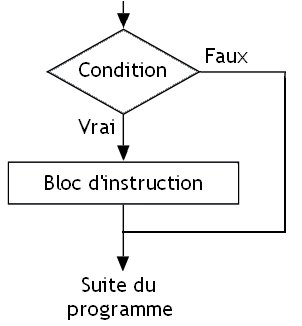
\includegraphics[scale=0.4]{images/boucle_condition.jpg}
\caption{Structure If}
\end{figure}

L'instruction \mybox{if} ressemble à ceci.

\begin{C}
if (/* Condition */)
{
    /* Une ou plusieurs instruction(s) */
}
\end{C}

Si la condition n'est pas vérifiée, le bloc d'instructions est passé et
le programme recommence immédiatement à la suite du bloc d'instructions
délimité par l'instruction \mybox{if}.

Si vous n'avez qu'une seule instruction à réaliser, vous avez la
possibilité de ne pas mettre d'accolades.

\begin{C}
if (/* Condition */)
    /* Une seule instruction */
\end{C}

Cependant, nous vous conseillons de mettre les accolades
systématiquement afin de vous éviter des problèmes si vous décidez de
rajouter des instructions par la suite en oubliant d'ajouter des
accolades. Bien sûr, ce n'est qu'un conseil, vous êtes libre de ne pas
le suivre.

À présent, voyons quelques exemples d'utilisation.

\subsubsection{Exemple 1}
\label{exemple-1}

\begin{C}
#include <stdio.h>


int main(void)
{
    int a = 10;
    int b = 20;

    if (a < b)
    {
        printf("%d est inférieur à %d\n", a, b);
    }

    return 0;
}
\end{C}

\begin{C}
10 est inférieur à 20
\end{C}

L'instruction \mybox{if} évalue l'expression logique
\mybox{a\ \textless{}\ b}, conclut qu'elle est valide et exécute le
bloc d'instructions.

\subsubsection{Exemple 2}
\label{exemple-2}

\begin{C}
#include <stdio.h>


int main(void)
{
    int a = 10;
    int b = 20;

    if (a > b)
    {
        printf("%d est supérieur à %d\n", a, b);
    }

    return 0;
}
\end{C}

Ce code n'affiche rien. La condition étant fausse, le bloc contenant
l'appel à la fonction \mybox{printf()} est ignoré.

\subsection{L'instruction else}
\label{linstruction-else}

Avec l'instruction \mybox{if}, nous savons exécuter un bloc
d'instructions quand une condition est remplie. Toutefois, si nous
souhaitons réaliser une action en cas d'échec de l'évaluation de la
condition, nous devons ajouter une autre instruction \mybox{if} à la
suite, comme ci-dessous.

\begin{C}
if (a > 5)
{
    /* Du code */
}

if (a <= 5)
{
    /* Code alternatif */
}
\end{C}

Le seul problème, c'est qu'il est nécessaire d'ajouter une instruction
\mybox{if} et d'évaluer une nouvelle condition, ce qui n'est pas très
efficace et assez long à taper. Pour limiter les dégâts, le C fournit
une autre instruction : \mybox{else}, qui signifie « sinon ». Celle-ci
se place immédiatement après le bloc d'une instruction \mybox{if} et
permet d'exécuter un bloc d'instructions alternatif si la condition
testée n'est pas vérifiée. Sa syntaxe est la suivante.

\begin{C}
if (/* Condition */)
{
    /* Une ou plusieurs instructions */
}
else
{
    /* Une ou plusieurs instructions */
}
\end{C}

Et elle doit être comprise comme ceci.

\begin{figure}[htbp]
\centering
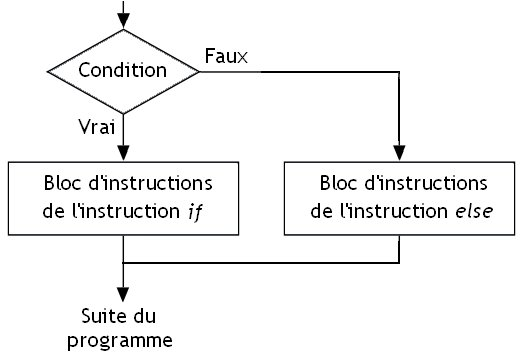
\includegraphics[scale=0.4]{images/boucle_if_else.jpg}
\caption{Structure if else}
\end{figure}

\begin{infobox} Notez que l'instruction \mybox{else}
ne possède aucune parenthèse.
\end{infobox}

\subsection{Exemple}
\label{exemple-3}

Supposons que nous voulions créer un programme très simple auquel nous
fournissons une heure et qui indique s'il fait jour ou nuit à cette
heure-là. Nous supposerons qu'il fait jour de 8 heures à 20 heures et
qu'il fait nuit sinon.

\begin{C}
int main(void)
{
    int heure;
    scanf("%d", &heure);

    if (heure > 8 && heure < 20)
    {
        printf("Il fait jour.\n");
    }
    else
    {
        printf("Il fait nuit.\n");
    }

    return 0;
}
\end{C}

\begin{C}
10
Il fait jour.
\end{C}

\section{If / else if}
\label{if-else-if}

Il est parfois nécessaire d'imbriquer plusieurs instructions \mybox{if}
et \mybox{else} les unes dans les autres.

\begin{C}
if (/* Condition */)
{
    /* Du code */
}
else
{
    /* Une ou plusieurs instruction(s) */

    if (/* Autre condition */)
    {
        /* Du code */
    }
}
\end{C}

Cependant, c'est assez long à écrire, d'autant plus s'il y a beaucoup
d'imbrications. Pour éviter ces inconvénients, sachez qu'il est possible
de combiner une instruction \mybox{else} et une instruction
\mybox{if}. Les imbrications simplifiables avec une suite \mybox{else}
\mybox{if} sont celles qui s'écrivent comme suit.

\begin{C}
if (/* Expression logique */)
{
    /* Une ou plusieurs instruction(s) */
}
else 
{
    if (/* Expression logique */)
    {
        /* Une ou plusieurs instruction(s) */
    }
}
\end{C}

Faites bien attention : le bloc d'instructions du \mybox{else} doit
contenir un \mybox{if}, éventuellement avec un \mybox{else}, mais rien
d'autre. Celles-ci peuvent alors être simplifiées comme ceci.

\begin{C}
if (/* Expression logique */)
{
    /* Une ou plusieurs instruction(s) */
}
else if (/* Expression logique */)
{
    /* Une ou plusieurs instruction(s) */
}
\end{C}

Comme vous pouvez le voir, nous avons « fusionné » l'instruction
\mybox{else} et la seconde instruction \mybox{if}. Notez que comme il
s'agit toujours d'une suite d'instructions \mybox{if} et \mybox{else},
il n'y aura qu'un seul bloc d'instructions qui sera finalement exécuté.
En effet, l'ordinateur va tester la condition de l'instruction
\mybox{if}, puis, si elle est fausse, celle de l'instruction
\mybox{if} suivant l'instuction \mybox{else} et ainsi de suite jusqu'à
ce qu'une condition soit vraie (ou jusqu'à une instruction \mybox{else}
finale si elles sont toutes fausses).

\begin{infobox} Notez qu'il n'est pas obligatoire
d'ajouter une instruction \mybox{else}.
\end{infobox}

\begin{C}
#include <stdio.h>


int main(void)
{
    int heure = 11;

    if (heure < 7)
    {
        printf("Zzz... \n");
    }
    else if (heure >= 7 && heure < 12)
    {
        printf("C'est le matin !\n");
    }
    else if (heure == 12)
    {
        printf("Il est midi !\n");
    }
    else if (heure > 12 && heure < 18)
    {
        printf("C'est l'après-midi !\n");
    }
    else if (heure >= 18 && heure < 24)
    {
        printf("C'est le soir !\n");
    }
    else if (heure == 24 || heure == 0)
    {
        printf("Il est minuit, dormez brave gens !\n");
    }
    else
    {
        printf("Il est l'heure de réapprendre à lire l'heure !\n");
    }

    return 0;

\end{C}

\begin{C}
11
On est le matin !
0
Il est minuit, dormez brave gens !
-2
Il est l'heure de réapprendre à lire l'heure !
\end{C}

\subsection{Exercice}
\label{exercice-1}

Imaginez que vous avez un score de jeu vidéo sous la main :

\begin{itemize}
\item
  si le score est strictement inférieur à deux mille, affichez « C'est
  la catastrophe ! » ;
\item
  si le score est supérieur ou égal à deux mille et que le score est
  strictement inférieur à cinq mille, affichez : « Tu peux mieux faire
  ! » ;
\item
  si le score est supérieur ou égal à cinq mille et que le score est
  strictement inférieur à neuf mille, affichez : « Tu es sur la bonne
  voie ! » ;
\item
  sinon, affichez : « Tu es le meilleur ! ».
\end{itemize}

Au boulot !

\begin{C}
 #include <stdio.h>


int main(void)
{
    int score;

    printf("Quel est le score du joueur ? ");
    scanf("%d", &score);

    if (score < 2000)
    {
        printf("C'est la catastrophe !\n");
    }
    else if (score >= 2000 && score < 5000)
    {
        printf("Tu peux mieux faire !\n");
    }
    else if (score >= 5000 && score < 9000)
    {
        printf("Tu es sur la bonne voie !\n");
    }
    else
    {
        printf("Tu es le meilleur !\n");
    }

    return 0;
}
\end{C}


\section{L'instruction switch}
\label{linstruction-switch}

L'instruction \mybox{switch} permet de comparer la valeur d'une
variable par rapport à une liste de valeurs. Techniquement, elle permet
d'écrire de manière plus concise une suite d'instructions \mybox{if} et
\mybox{else} qui auraient pour objectif d'accomplir différentes actions
suivant la valeur d'une variable.

\begin{C}
if (a == 1)
{
    /* Instruction(s) */
}
else if (a == 2)
{
    /* Instruction(s) */
}
/* Etc. */
else
{
    /* Instruction(s) */
}
\end{C}

Avec l'instruction \mybox{switch}, cela donne ceci.

\begin{C}
switch (a)
{
case 1:
    /* Instruction(s) */
    break;
case 2:
    /* Instruction(s) */
    break;

/* Etc... */

default: /* Si aucune comparaison n'est juste */
    /* Instruction(s) à exécuter dans ce cas */
    break;
}
\end{C}

Ici, la valeur de la variable \emph{a} est comparée successivement avec
chaque entrée de la liste, indiquées par le mot-clé \mybox{case}. En
cas de correspondance, les instructions suivant le mot-clé \mybox{case}
sont exécutées jusqu'à rencontrer une instruction \mybox{break} (nous
la verrons plus en détail un peu plus tard). Si aucune comparaison n'est
bonne, alors ce sont les instructions de l'entrée marquée avec le
mot-clé \mybox{default} qui seront exécutées.

\subsection{Exemple}
\label{exemple-4}

\begin{C}
#include <stdio.h>


int main(void)
{
    int note;

    printf("Quelle note as-tu obtenue (sur cinq) ? ");
    scanf("%d", &note);

    switch(note)
    {
    /* si note == 0 */
    case 0:
        printf("No comment.\n");
        break;

    /* si note == 1 */
    case 1:
        printf("Cela te fait 4/20, c'est accablant.\n");
        break;

    /* si note == 2 */   
    case 2:
        printf("On se rapproche de la moyenne, mais ce n'est pas encore ça.\n");
        break;

    /* si note == 3 */
    case 3:
        printf("Tu passes.\n");
        break;

    /* si note == 4*/
    case 4:
        printf("Bon travail, continue ainsi !\n");
        break;

    /* si note == 5 */
    case 5:
        printf("Excellent !\n");
        break;

    /* si note est différente de 0, 1, 2, 3, 4 et 5 */
    default:
        printf("Euh... tu possèdes une note improbable...\n");
        break;
    }

    return 0;
}
\end{C}

\begin{infobox} Notez que comme pour l'instruction
\mybox{else}, une entrée marquée avec le mot-clé \mybox{default} n'est
pas obligatoire.
\end{infobox}

\subsection{Plusieurs entrées pour une même action}
\label{plusieurs-entrees-pour-une-muxeame-action}

Une même suite d'instructions pour être désignée par plusieurs entrées
comme le montre l'exemple suivant.

\begin{C}
int main(void)
{
    int note;

    printf("Quelle note as-tu obtenue ? ");
    scanf("%d", &note);

    switch(note)
    {
    /* si la note est comprise entre zéro et trois inclus */
    case 0:
    case 1:
    case 2:
    case 3:
        printf("No comment.\n");
        break;

    /* si la note est comprise entre quatre et sept inclus */
    case 4:
    case 5:
    case 6:
    case 7:
        printf("C'est accablant.\n");
        break;

    /* si la note est comprise entre huit et neuf inclus */  
    case 8:
    case 9:
        printf("On se rapproche de la moyenne, mais ce n'est pas encore ça.\n");
        break;

    /* si la note est comprise entre dix et douze inclus */
    case 10:
    case 11:
    case 12:
        printf("Tu passes.\n");
        break;

    /* si la note est comprise entre treize et seize inclus */
    case 13:
    case 14:
    case 15:
    case 16:
        printf("Bon travail, continue ainsi !\n");
        break;

    /* si la note est comprise entre dix-sept et vingt inclus */
    case 17:
    case 18:
    case 19:
    case 20:
        printf("Excellent !\n");
        break;

    /* si la note est différente */
    default:
        printf("Euh... tu possèdes une note improbable...\n");
        break;
    }

    return 0;
}
\end{C}

\section{Plusieurs entrées sans instruction break}
\label{plusieurs-entrees-sans-instruction-break}

Si vous l'utiliserez souvent, sachez également que l'instruction
\mybox{break} n'est pas obligatoire. En effet, le but de cette dernière
est de sortir du \mybox{switch} et donc de ne pas exécuter les actions
d'autre entrées. Toutefois, il arrive que les actions à réaliser se
chevauchent entre entrées auquel cas l'instruction \mybox{break} serait
plutôt mal venue.

Prenons un exemple : vous souhaitez réaliser un programme qui affiche
entre 1 à dix fois la même phrase, ce nombre étant fourni par
l'utilisateur. Vous pourriez écrire une suite de \mybox{if} ou
différentes entrées d'un \mybox{switch} qui, suivant le nombre entré,
appelleraient une fois \mybox{printf()}, puis deux fois, puis trois
fois, etc. mais cela serait horriblement lourd.

Dans un tel cas, une meilleure solution consiste à appeler
\mybox{printf()} à chaque entrée du \mybox{switch}, mais de ne pas
terminer ces dernières par une instruction \mybox{break}.

\begin{C}
#include <stdio.h>


int
main(void)
{
    unsigned nb;

    printf("Combien de fois souhaitez-vous répéter l'affichage (entre 1 à 10 fois) ? ");
    scanf("%u", &nb);

    switch (nb)
    {
    case 10:
        printf("Cette phrase est répétée une à dix fois.\n");
    case 9:
        printf("Cette phrase est répétée une à dix fois.\n");
    case 8:
        printf("Cette phrase est répétée une à dix fois.\n");
    case 7:
        printf("Cette phrase est répétée une à dix fois.\n");
    case 6:
        printf("Cette phrase est répétée une à dix fois.\n");
    case 5:
        printf("Cette phrase est répétée une à dix fois.\n");
    case 4:
        printf("Cette phrase est répétée une à dix fois.\n");
    case 3:
        printf("Cette phrase est répétée une à dix fois.\n");
    case 2:
        printf("Cette phrase est répétée une à dix fois.\n");
    case 1:
        printf("Cette phrase est répétée une à dix fois.\n");
    case 0:
        break;
    default:
        printf("Certes, mais encore ?\n");
        break;
    }

    return 0;
}
\end{C}

\begin{C}
Combien de fois souhaitez-vous répéter l'affichage (entre 1 à 10 fois) ? 2
Cette phrase est répétée une à dix fois.
Cette phrase est répétée une à dix fois.

Combien de fois souhaitez-vous répéter l'affichage (entre 1 à 10 fois) ? 5
Cette phrase est répétée une à dix fois.
Cette phrase est répétée une à dix fois.
Cette phrase est répétée une à dix fois.
Cette phrase est répétée une à dix fois.
Cette phrase est répétée une à dix fois.
\end{C}

Comme vous le voyez, la phrase « Cette phrase est répétée une à dix fois
» est affichée une à dix fois suivant le nombre initialement fourni.
Cela est possible étant donné l'absence d'instruction \mybox{break}
entre les \mybox{case} 10 à 1, ce qui fait que l'exécution du
\mybox{switch} continue de l'entrée initiale jusqu'au \mybox{case} 0.

\section{L'opérateur conditionnel}
\label{loperateur-conditionnel}

L'\textbf{opérateur conditionnel} ou \textbf{opérateur ternaire} est un opérateur
particulier dont le résultat dépend de la réalisation d'une condition.
Son deuxième nom lui vient du fait qu'il est le seul opérateur du
langage C à requérir trois opérandes : une condition et deux
expressions.

\begin{C}
(condition) ? expression si vrai : expression si faux
\end{C}

\begin{infobox}
Les parenthèses entourant la
condition ne sont pas obligatoires, mais préférables.
\end{infobox}

\emph{Grosso modo}, cet opérateur permet d'écrire de manière condensée
une structure \mybox{if\ \{\}\ else\ \{\}}. Voyez par vous-mêmes.

\begin{C}
#include <stdio.h>

int main(void)
{
    int heure;

    scanf("%d", &heure);

    (heure > 8 && heure < 20) ? printf("Il fait jour.\n") : printf("Il fait nuit.\n");
    return 0;
}
\end{C}

Il est également possible de l'écrire sur plusieurs lignes, même si
cette pratique est moins courante.

\begin{C}
(heure > 8 && heure < 20)
    ? printf("Il fait jour.\n")
    : printf("Il fait nuit.\n");
\end{C}

Cet opérateur peut sembler inutile de prime abord, mais il s'avère être
un allié de choix pour simplifier votre code quand celui-ci requiert la
vérification de conditions simples.

\subsection{Exercice}
\label{exercice-2}

Pour bien comprendre cette nouvelle notion, nous allons faire un petit
exercice. Imaginez que nous voulions faire un mini jeu vidéo dans lequel
nous affichons le nombre de coups du joueur. Seulement voilà, vous êtes
maniaques du français et vous ne supportez pas qu'il y ait un « s » en
trop ou en moins. Essayez de réaliser un programme qui demande à
l'utilisateur d'entrer un nombre de coups puis qui affiche celui-ci
correctement accordé.

\begin{C}
 #include <stdio.h>

int main(void)
{
    int nb_coups;

    printf("Donnez le nombre de coups : ");
    scanf("%d", &nb_coups);
    printf("Vous gagnez en %d coup%c\n", nb_coups, (nb_coups > 1) ? 's' : ' ');
    return 0;
}
\end{C}

Ce programme utilise l'opérateur conditionnel pour condenser
l'expression et aller plus vite dans l'écriture du code. Sans lui nous
aurions dû écrire quelque chose comme ceci.

\begin{C}
 #include <stdio.h>

int main(void)
{
    int nb_coups;

    printf("Donnez le nombre de coups : ");
    scanf("%d", &nb_coups);

    if (nb_coups > 1)
        printf("Vous gagnez en %d coups\n", nb_coups);
    else
        printf("Vous gagnez en %d coup\n", nb_coups);

    return 0;
}
\end{C}

Ce chapitre a été important, il vous a permis d’utiliser les conditions ; les instructions \mybox{if} et \mybox{else};
l’instruction \mybox{switch} et l'opérateur conditionnel. Aussi, si vous n'avez pas très bien compris
ou que vous n'avez pas tout retenu, nous vous conseillons de relire ce
chapitre.

Le chapitre suivant sera l'occasion de mettre en œuvre ce que vous avez
appris puisqu'il s'agira de votre premier TP.

*{[}TP{]}: Travaux Pratiques
\chapter{TP : déterminer le jour de la semaine}
\label{TP-:-determiner-le-jour-de-la-semaine }

Avant de poursuivre notre périple, il est à présent temps de nous poser un
instant afin de réaliser un petit exercice reprenant tout ce qui vient
d'être vu.

\section{Objectif}
\label{objectif }

Votre objectif est de parvenir à réaliser un programme qui,
suivant une date fournie par l'utilisateur sous la forme « jj/mm/aaaa »,
donne le jour de la semaine correspondant. Autrement dit, voici ce que
devrait donner l'exécution de ce programme.

\begin{C}
Entrez une date : 11/2/2015
C'est un mercredi

Entrez une date : 13/7/1970
C'est un lundi
\end{C}

\section{Première étape}
\label{premiere-etape }

Pour cette première étape, vous allez devoir réaliser un programme qui
demande à l'utilisateur un jour du mois de janvier de l'an un et qui lui
précise de quel jour de la semaine il s'agit, le tout à l'aide de la
méthode présentée ci-dessous.

\begin{C}
Entrez un jour : 27
C’est un jeudi
\end{C}

\subsection{Déterminer le jour de la semaine}
\label{determiner-le-jour-de-la-semaine}

Pour déterminer le jour de la semaine correspondant à une date, vous
allez devoir partir du premier janvier de l'an un (c'était un samedi) et
calculer le nombre de jours qui sépare cette date de celle fournie par
l'utilisateur. Une fois ce nombre obtenu, il nous est possible d'obtenir
le jour de la semaine correspondant à l'aide de l'opérateur modulo.

En effet, comme vous le savez, les jours de la semaine suivent un cycle
et se répètent tous les sept jours. Or, le reste de la division entière
est justement un nombre cyclique allant de zéro jusqu'au diviseur
diminué de un. Voici ce que donne le reste de la division entière des
chiffres 1 à 9 par 3.

\begin{C}
1 % 3 = 1
2 % 3 = 2
3 % 3 = 0
4 % 3 = 1
5 % 3 = 2
6 % 3 = 0
7 % 3 = 1
8 % 3 = 2
9 % 3 = 0
\end{C}

Comme vous le voyez, le reste de la division oscille toujours entre zéro
et deux. Ainsi, si nous attribuons un chiffre de zéro à six à chaque
jour de la semaine (par exemple zéro pour samedi et ainsi de suite pour
les autres) nous pouvons déduire le jour de la semaine correspondant à
un nombre de jours depuis le premier janvier de l'an un.

Prenons un exemple : l'utilisateur entre la date du vingt-sept janvier
de l'an un. Il y a vingt-six jours qui le sépare du premier janvier. Le
reste de la division entière de vingt-six par 7 est 5, il s'agit donc
d'un jeudi.

Si vous le souhaitez, vous pouvez vous aider du calendrier suivant.

\begin{C}
     Janvier 1        
di lu ma me je ve sa  
                   1  
 2  3  4  5  6  7  8  
 9 10 11 12 13 14 15  
16 17 18 19 20 21 22  
23 24 25 26 27 28 29  
30 31
\end{C}

À présent, à vous de jouer. ;)

\section{Correction}
\label{correction-1}

Alors, cela s'est bien passé ? Si oui, félicitations, si non, la
correction devrait vous aider à y voir plus clair.

\begin{C}
 #include <stdio.h>


int
main(void)
{
    unsigned jour;
    int njours;

    printf("Entrez un jour : ");
    scanf("%u", &jour);

    njours = (jour - 1);

    switch (njours % 7)
    {
    case 0:
        printf("C'est un samedi\n");
        break;

    case 1:
        printf("C'est un dimanche\n");
        break;

    case 2:
        printf("C'est un lundi\n");
        break;

    case 3:
        printf("C'est un mardi\n");
        break;

    case 4:
        printf("C'est un mercredi\n");
        break;

    case 5:
        printf("C'est un jeudi\n");
        break;

    case 6:
        printf("C'est un vendredi\n");
        break;
    }
    
    return 0;
}
\end{C}

Tout d'abord, nous demandons à l'utilisateur d'entrer un jour du mois de
janvier que nous affectons à la variable \mybox{jour}. Ensuite, nous
calculons la différence de jours séparant le premier janvier de celui
entré par l'utilisateur. Enfin, nous appliquons le modulo à ce résultat
afin d'obtenir le jour de la semaine correspondant.

\section{Deuxième étape}
\label{deuxieme-etape }

Bien, complexifions à présent un peu notre programme
et demandons à l'utilisateur de nous fournir un jour \emph{et} un mois
de l'an un.

\begin{C}
Entrez une date (jj/mm) : 20/4
C'est un mercredi
\end{C}

Pour ce faire, vous allez devoir convertir chaque mois en son nombre de
jours et ajouter ensuite celui-ci au nombre de jours séparant la date
entrée du premier du mois. À cette fin, vous pouvez considérer dans un
premier temps que chaque mois compte trente et un jours et ensuite
retrancher les jours que vous avez compté en trop suivant le mois
fourni.

Par exemple, si l'utilisateur vous demande quel jour de la semaine était
le vingt avril de l'an un :

\begin{itemize}
\item
  vous multipliez trente et un par trois puisque trois mois séparent le
  mois d'avril du mois de janvier (janvier, février et mars) ;
\item
  vous retranchez trois jours (puisque le mois de février ne comporte
  que vingt-huit jours les années non bissextiles) ;
\item
  enfin, vous ajoutez les dix-neuf jours qui séparent la date fournie du
  premier du mois.
\end{itemize}

Au total, vous obtenez alors cent et neuf jours, ce qui nous donne,
modulo sept, le nombre quatre, c'est donc un mercredi.

À toutes fins utiles, voici le calendrier complet de l'an un.

\begin{C}
  Janvier               Février                 Mars          
di lu ma me je ve sa  di lu ma me je ve sa  di lu ma me je ve sa  
                   1         1  2  3  4  5         1  2  3  4  5  
 2  3  4  5  6  7  8   6  7  8  9 10 11 12   6  7  8  9 10 11 12  
 9 10 11 12 13 14 15  13 14 15 16 17 18 19  13 14 15 16 17 18 19  
16 17 18 19 20 21 22  20 21 22 23 24 25 26  20 21 22 23 24 25 26  
23 24 25 26 27 28 29  27 28                 27 28 29 30 31        
30 31                                                             

       Avril                  Mai                   Juin          
di lu ma me je ve sa  di lu ma me je ve sa  di lu ma me je ve sa  
                1  2   1  2  3  4  5  6  7            1  2  3  4  
 3  4  5  6  7  8  9   8  9 10 11 12 13 14   5  6  7  8  9 10 11  
10 11 12 13 14 15 16  15 16 17 18 19 20 21  12 13 14 15 16 17 18  
17 18 19 20 21 22 23  22 23 24 25 26 27 28  19 20 21 22 23 24 25  
24 25 26 27 28 29 30  29 30 31              26 27 28 29 30        
                                                                  

      Juillet                 Août               Septembre        
di lu ma me je ve sa  di lu ma me je ve sa  di lu ma me je ve sa  
                1  2      1  2  3  4  5  6               1  2  3  
 3  4  5  6  7  8  9   7  8  9 10 11 12 13   4  5  6  7  8  9 10  
10 11 12 13 14 15 16  14 15 16 17 18 19 20  11 12 13 14 15 16 17  
17 18 19 20 21 22 23  21 22 23 24 25 26 27  18 19 20 21 22 23 24  
24 25 26 27 28 29 30  28 29 30 31           25 26 27 28 29 30     
31                                                                

      Octobre               Novembre              Décembre        
di lu ma me je ve sa  di lu ma me je ve sa  di lu ma me je ve sa  
                   1         1  2  3  4  5               1  2  3  
 2  3  4  5  6  7  8   6  7  8  9 10 11 12   4  5  6  7  8  9 10  
 9 10 11 12 13 14 15  13 14 15 16 17 18 19  11 12 13 14 15 16 17  
16 17 18 19 20 21 22  20 21 22 23 24 25 26  18 19 20 21 22 23 24  
23 24 25 26 27 28 29  27 28 29 30           25 26 27 28 29 30 31  
30 31
\end{C}

À vos claviers !

\section{Correction}
\label{correction-2}

Bien, passons à la correction.

\begin{C}
 #include <stdio.h>


int
main(void)
{
    unsigned jour;
    unsigned mois;
    int njours;

    printf("Entrez une date (jj/mm) : ");
    scanf("%u/%u", &jour, &mois);

    njours = (mois - 1) * 31;

    switch (mois)
    {
    case 12:
        --njours;
    case 11:
    case 10:
        --njours;
    case 9:
    case 8:
    case 7:
        --njours;
    case 6:
    case 5:
        --njours;
    case 4:
    case 3:
        njours -= 3;
        break;
    }

    njours += (jour - 1);

    switch (njours % 7)
    {
    case 0:
        printf("C'est un samedi\n");
        break;

    case 1:
        printf("C'est un dimanche\n");
        break;

    case 2:
        printf("C'est un lundi\n");
        break;

    case 3:
        printf("C'est un mardi\n");
        break;

    case 4:
        printf("C'est un mercredi\n");
        break;

    case 5:
        printf("C'est un jeudi\n");
        break;

    case 6:
        printf("C'est un vendredi\n");
        break;
    }

    return 0;
}
\end{C}

Nous commencons par demander deux nombres à l'utilisateur qui sont
affectés aux variables \mybox{jours} et \mybox{mois}. Ensuite, nous
multiplions le nombre de mois séparant celui entré par l'utilisateur du
mois de janvier par trente et un. Après quoi, nous soustrayons les jours
comptés en trop suivant le mois fourni. Enfin, nous ajoutons le nombre
de jours séparant celui entré du premier du mois, comme pour la première
étape.

\begin{infobox}
Notez que nous avons utilisé ici une
propriété intéressante de l'instruction \mybox{switch} : si la valeur
de contrôle correspond à celle d'une entrée, alors les instructions sont
exécutées \emph{jusqu'à rencontrer une instruction} \mybox{break} (ou
jusqu'à la fin du \mybox{switch}). Ainsi, si le mois entré est celui de
mai, l'instruction \mybox{$-$$-$njours} va être exécutée, puis
l'instruction \mybox{njours $-$= 3} va également être exécutée. 
\end{infobox}

\section{Troisième et dernière étape}
\label{troisieme-et-derniere-etape }

À présent, il est temps de réaliser un programme complet qui correspond aux objectifs du TP. Vous
allez donc devoir demander à l'utilisateur une date entière et lui
donner le jour de la semaine correspondant.

\begin{C}
Entrez une date : 11/2/2015
C'est un mercredi
\end{C}

Toutefois, avant de vous lancer dans la réalisation de celui-ci, nous
allons parler calendriers et années bissextiles.

\subsection{Les calendriers Julien et Grégorien}
\label{les-calendriers-julien-et-gregorien}

Vous le savez certainement, une
\MYhref{http://fr.wikipedia.org/wiki/Ann\%C3\%A9e_bissextile}{année
bissextile} est une année qui comporte 366 jours au lieu de 365 et qui
se voit ainsi ajouter un vingt-neuf février. Ce que vous ne savez en
revanche peut-être pas, c'est que la détermination des années bissextile
a varié au cours du temps.

Jusqu'en 1582, date d'adoption du
\MYhref{http://fr.wikipedia.org/wiki/Calendrier_gr\%C3\%A9gorien}{calendrier
Grégorien} (celui qui est en vigueur un peu près partout actuellement),
c'est le
\MYhref{http://fr.wikipedia.org/wiki/Calendrier_julien}{calendrier Julien}
qui était en application. Ce dernier considérait une année comme
bissextile si celle-ci était multiple de quatre. Cette méthode serait
correcte si une année comportait 365,25 jours. Cependant, il s'est avéré
plus tard qu'une année comportait en fait 365,2422 jours.

Dès lors, un décalage par rapport au cycle terrestre s'était lentement
installé ce qui posa problème à l'Église catholique pour le calcul de la
date de Pâques qui glissait doucement vers l'été. Le calendrier
Grégorien fût alors instauré en 1582 pour corriger cet écart en
modifiant la règle de calcul des années bissextile : il s'agit d'une
année multiple de quatre \emph{et}, s'il s'agit d'une année multiple de
100, également multiple de 400. Par exemple, les années 1000 et 1100 ne
sont plus bissextiles à l'inverse de l'année 1200 qui, elle, est
divisible par 400.

Toutefois, ce ne sont pas douze années bissextiles qui ont été
supprimées lors de l'adoption du calendrier Grégorien (100, 200, 300,
500, 600, 700, 900, 1000, 1100, 1300, 1400, 1500), mais seulement dix
afin de rapprocher la date de Pâques de l'équinoxe de printemps.

\subsection{Mode de calcul}
\label{mode-de-calcul}

Pour réaliser votre programme, vous devrez donc vérifier si la date
demandée est antérieure ou postérieure à l'an 1582. Si elle est
inférieure ou égale à l'an 1582, alors vous devrez appliquer le
calendrier Julien. Si elle est supérieure, vous devrez utiliser le
calendrier Grégorien.

Pour vous aider, voici un schéma que vous pouvez suivre.

\begin{C}
Si l'année est supérieure à 1582
    Multipler la différence d'années par 365
    Ajouter au résultat le nombre d'années multiples de 4
    Soustraire à cette valeur le nombre d'années multiples de 100
    Ajouter au résultat le nombre d'années multiples de 400
    Ajouter deux à ce nombre (du fait que seules dix années ont été supprimées en 1582)
Si l'année est inférieure ou égale à 1582
    Multipler la différence d'années par 365
    Ajouter au résultat le nombre d'années multiples de 4

Au nombre de jours obtenus, ajouter la différence de jours entre
le mois de janvier et le mois fourni. N'oubliez pas que les mois comportent
trente et un ou trente jours et que le mois de février comporte pour sa
part vingt-huit jours sauf les années bisextiles où il s'en voit ajouter un
vingt-neuvième. Également, faites attention au calendrier en application pour
la détermination des années bissextiles !

Au résultat obtenu ajouter le nombre de jour qui sépare celui entré du premier
du mois.

Appliquer le modulo et déterminer le jour de la semaine.
\end{C}

À vous de jouer !

\section{Correction}
\label{correction-3}

Ça va, vous tenez bon ?

\begin{C}
 #include <stdio.h>


int
main(void)
{
    unsigned jour;
    unsigned mois;
    unsigned an;
    int njours;

    printf("Entrez une date (jj/mm/aaaa) : ");
    scanf("%u/%u/%u", &jour, &mois, &an);
    njours = (an - 1) * 365;

    if (an > 1582) /* Calendrier Grégorien */
    {
        njours += ((an - 1) / 4);
        njours -= ((an - 1) / 100);
        njours += ((an - 1) / 400);
        njours += 2;
    }
    else /* Calendrier Julien */
        njours += ((an - 1) / 4);

    njours += (mois - 1) * 31;

    switch (mois)
    {
    case 12:
        --njours;
    case 11:
    case 10:
        --njours;
    case 9:
    case 8:
    case 7:
        --njours;
    case 6:
    case 5:
        --njours;
    case 4:
    case 3:
        if (an > 1582)
        {
            if (an % 4 == 0 && (an % 100 != 0 || an % 400 == 0))
                njours -= 2;
            else
                njours -= 3;
        }
        else
        {
            if (an % 4 == 0)
                njours -= 2;
            else
                njours -= 3;
        }
        break;
    }


    njours += (jour - 1);

    switch (njours % 7)
    {
    case 0:
        printf("C'est un samedi\n");
        break;

    case 1:
        printf("C'est un dimanche\n");
        break;

    case 2:
        printf("C'est un lundi\n");
        break;

    case 3:
        printf("C'est un mardi\n");
        break;

    case 4:
        printf("C'est un mercredi\n");
        break;

    case 5:
        printf("C'est un jeudi\n");
        break;

    case 6:
        printf("C'est un vendredi\n");
        break;
    }
    
    return 0;
}
\end{C}

Tout d'abord, nous demandons à l'utilisateur d'entrer une date au format
jj/mm/aaaa et nous attribuons chaque partie aux variables \mybox{jour},
\mybox{mois} et \mybox{an}. Ensuite, nous multiplions par 365 la
différence d'années séparant l'année fournie de l'an un. Toutefois, il
nous faut encore prendre en compte les années bissextiles pour que le
nombre de jours obtenus soit correct. Nous ajoutons donc un jour par
année bissextile en prenant soin d'appliquer les règles du calendrier en
vigueur à la date fournie.

Maintenant, il nous faut ajouter le nombre de jours séparant le mois de
janvier du mois spécifié par l'utilisateur. Pour ce faire, nous
utilisons la même méthode que celle vue lors de la deuxième étape
\emph{à une différence près} : nous vérifions si l'année courante est
bissextile afin de retrancher le bon nombre de jours (le mois de février
comportant dans ce cas vingt-neuf jours et non vingt-huit).

Enfin, nous utilisons le même code que celui de la première étape.



\hrulefill

Ce chapitre nous aura permis de faire une petite pause et de mettre en application ce que nous
avons vu dans les chapitres précédents. Reprenons à présent notre route
en attaquant la notion de \textbf{boucle}.
\chapter{Les boucles}
\label{les-boucles}

Dans ce chapitre, nous allons aborder les \textbf{boucles}.
Une boucle est un moyen de répéter des instructions
suivant le résultat d'une condition. Ces structures, dîtes
\textbf{itératives}, que nous allons voir dans ce chapitre sont les
suivantes.

\begin{table}
\centering
\rowcolors{1}{gris-clair-tab}{}
\begin{tabular}{|p{3cm}|p{12cm}|}\hline
\rowcolor{gris-tab-entete}\textbf{\makecell{Structure \\itérative}} & \textbf{\makecell{Action}}\tabularnewline\hline
\textbf{\emph{while\ldots{}}} & répète une suite d'instructions tant qu'une condition est respectée.\tabularnewline\hline
\textbf{\emph{do\ldots{} while\ldots{}}} & répète une suite d'instructions tant qu'une condition est respectée. Le groupe d'instructions est exécuté au moins une fois.\tabularnewline\hline
\textbf{\emph{for\ldots{}}} &  répète un nombre fixé de fois une suite d'instructions.\tabularnewline\hline
\end{tabular}
\end{table}

\section{La boucle while}
\label{la-boucle-while}

La première des boucles que nous allons étudier est la boucle
\mybox{while} (qui signifie « tant que »). Celle-ci permet de répéter
un bloc d'instructions tant qu'une condition est remplie.

\begin{figure}[htbp]
\centering
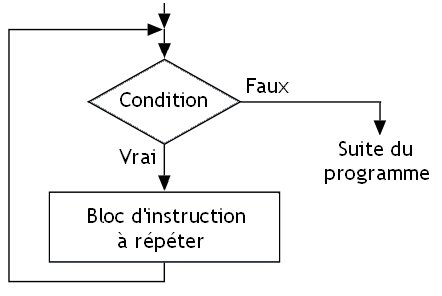
\includegraphics[scale=0.4]{images/structure-while.jpg}
\caption{Structure While}
\end{figure}

\subsection{Syntaxe}
\label{syntaxe-1}

La syntaxe de notre boucle \mybox{while} est assez simple.

\begin{C}
while (/* Condition */)
{
    /* Bloc d'instructions à répéter */ 
}
\end{C}

\subsubsection{Exemple}
\label{exemple-5}

\begin{C}
#include <stdio.h>


int main(void)
{
    int i = 0;

    while (i < 5)
    {
        printf("La variable i vaut %d\n", i);
        i++;
    }

    return 0;
}
\end{C}

\begin{C}
La variable i vaut 0
La variable i vaut 1
La variable i vaut 2
La variable i vaut 3
La variable i vaut 4
\end{C}

Le fonctionnement est simple à comprendre :

\begin{itemize}
\item
  Au départ, notre variable \mybox{i} vaut zéro. Étant donné que zéro
  est bien inférieur à cinq, la condition est vraie, le corps de la
  boucle est donc exécuté.
\item
  La valeur de \mybox{i} est affichée.
\item
  \mybox{i} est augmentée d'une unité et vaut désormais un.
\item
  La condition de la boucle est de nouveau vérifiée.
\end{itemize}

Ces étapes vont ainsi se répéter pour les valeurs un, deux, trois et
quatre. Quand la variable \mybox{i} vaudra cinq, la condition sera
fausse, et l'instruction \mybox{while} sera alors passée.

\begin{infobox}
  Dans cet exemple, nous utilisons une
variable nommée \mybox{i}. Ce nom lui vient d'une contraction du mot
anglais \emph{iterator} qui signifie que cette variable sert à
l'itération (la répétition) du corps de la boucle. Ce nom est tellement
court et explicite qu'il est pour ainsi dire devenu une convention de
nommage en C.
\end{infobox}

\subsection{Exercice}
\label{exercice-3}

Essayez de réaliser un programme qui détermine si un nombre entré par
l'utilisateur est premier. Pour rappel, un nombre est dit premier s'il
n'est divisible que par un et par lui-même. Notez que si un nombre \(x\)
est divisible par \(y\) alors le résultat de l'opération
\mybox{x\ \%\ y} est nul.

\subsubsection{Indice}
\label{indice-1}

\begin{secretbox}
 Pour savoir si un nombre est premier, il
va vous falloir vérifier si celui-ci est uniquement divisible par un et
lui-même. Dit autrement, vous allez devoir contrôler qu'aucun nombre
compris entre 1 et le nombre entré (tout deux exclus) n'est un diviseur
de ce dernier. Pour parcourir ces différentes possibilités, une boucle
va vous être nécessaire.
\end{secretbox}


\subsubsection{Correction}
\label{correction-4}

\begin{C}
 #include <stdio.h>


int main(void)
{
   int nombre;
   int i = 2;

   printf("Entrez un nombre : ");
   scanf("%d", &nombre);

   while ((i < nombre) && (nombre % i != 0))
   {
       ++i;
   }

   if (i == nombre)
   {
       printf("%d est un nombre premier\n", nombre);
   }
   else
   {
       printf("%d n'est pas un nombre premier\n", nombre);
   }

   return 0;
}
\end{C}

\section{La boucle do-while}
\label{la-boucle-do-while}

La boucle \mybox{do\ while} fonctionne comme la boucle \mybox{while},
à un petit détail près : elle s'exécutera toujours au moins une fois,
alors qu'une boucle \mybox{while} peut ne pas s'exécuter si la
condition est fausse dès le départ.

\begin{figure}[htbp]
\centering
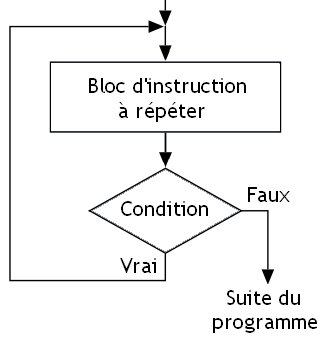
\includegraphics[scale=0.4]{images/instruction_do_while.jpg}
\caption{Instruction do\ldots{} while\ldots{}}
\end{figure}

\subsection{Syntaxe}
\label{syntaxe-2}

À la différence de la boucle \mybox{while}, la condition est placée à
la fin du bloc d'instruction à répéter, ce qui explique pourquoi
celui-ci est toujours exécuté au moins une fois. Remarquez également la
présence d'un point-virgule à la fin de l'instruction qui est
obligatoire.

\begin{C}
do
{
    /* Bloc d'instructions à répéter */
} while (/* Condition */);
\end{C}

\subsection{Exemple 1}
\label{exemple-6}

Voici le même code que celui présenté avec l'instruction \mybox{while}.

\begin{C}
#include <stdio.h>


int main(void)
{
    int i = 0;

    do
    {
        printf("La variable i vaut %d\n", i);
        ++i;
    } while (i < 5);

    return 0;
}
\end{C}

\begin{C}
La variable i vaut 0
La variable i vaut 1
La variable i vaut 2
La variable i vaut 3
La variable i vaut 4
\end{C}

\subsection{Exemple 2}
\label{exemple-7}

Comme nous vous l'avons dit plus haut, une boucle \mybox{do\ while}
s'éxecute au moins une fois.

\begin{C}
#include <stdio.h>


int main(void)
{    
    do
        printf("Boucle do-while\n");
    while (0);

    return 0;
}
\end{C}

\begin{C}
Boucle do-while
\end{C}

Comme vous le voyez, malgré que la condition est fausse (pour rappel,
une valeur nulle correspond à une valeur fausse), le corps de la boucle
est exécuté une fois puisque la condition n'est évaluée qu'\emph{après}
que le bloc d'instructions ait été parcouru.

\section{La boucle for}
\label{la-boucle-for}


\subsection{Syntaxe}
\label{syntaxe-3}

\begin{C}
for (/* Expression 1 */ ; /* Condition */ ; /* Expression 2 */)
{
    /* Instructions à répéter */
}
\end{C}

Une boucle \mybox{for} se décompose en trois parties :

\begin{itemize}
\item
  une expression, qui sera le plus souvent l'initialisation d'une
  variable ;
\item
  une condition ;
\item
  une seconde expression, qui consistera le plus souvent en
  l'incrémentation d'une variable.
\end{itemize}

Techniquement, une boucle \mybox{for} revient en fait à écrire ceci.

\begin{C}
/* Expression 1 */

while (/* Condition */)
{
    /* Bloc d'instructions à répéter */
    /* Expression 2 */
}
\end{C}

\subsection{Exemple}
\label{exemple-8}

Le fonctionnement de cette boucle est plus simple à appréhender à l'aide
d'un exemple.

\begin{C}
#include <stdio.h>


int main(void)
{
    int i;

    for (i = 0 ; i < 5 ; ++i)
        printf("la variable i vaut %d\n", i);

    return 0;
}
\end{C}

\begin{C}
variable vaut 0
variable vaut 1
variable vaut 2
variable vaut 3
variable vaut 4
\end{C}

Ce qui, comme dit précédemment, revient exactement à écrire cela.

\begin{C}
#include <stdio.h>


int main(void)
{
    int i;

    i = 0;

    while (i < 5)
    {
        printf("la variable i vaut %d\n", i);
        ++i;
    }

    return 0;
}
\end{C}

\begin{attentionbox}
  Notez bien que la première expression,
\mybox{i\ =\ 0}, est située \emph{en dehors} du corps de la boucle.
Elle n'est donc pas évaluée à chaque tour.
\end{attentionbox}

\subsubsection{Exercice}
\label{exercice-4}

Essayez de réaliser un programme qui calcule la somme de tous les
nombres compris entre un et \(n\) (\(n\) étant déterminé par vos soins).
Autrement dit, pour un nombre \(n\) donné, vous allez devoir calculer
\(1 + 2 + 3 + ... + (n-2) + (n-1) + n\).

\begin{C}
 #include <stdio.h>


int main (void)
{
    const unsigned int n = 250;
    unsigned int somme = 0;
    unsigned int i;

    for (i = 1; i <= n; ++i)
        somme += i;

    printf ("Somme de 1 à %u : %u\n", n, somme);
    return 0;
}
\end{C}

\begin{infobox}
 Notez qu'il est possible de réaliser
cet exercice sans boucle en calculant : \(\frac {N \times (N+1)} {2}\).
\end{infobox}

\subsection{Plusieurs compteurs}
\label{plusieurs-compteurs}

Notez que le nombre de compteurs ou de conditions n'est pas limité,
comme le démontre le code suivant.

\begin{C}
for (i = 0, j = 2 ; i < 10 && j < 12; i++, j += 2)
\end{C}

Ici, nous définissons deux compteurs \mybox{i} et \mybox{j}
initialisés respectivement à zéro et deux. Le contenu de la boucle est
exécuté tant que \mybox{i} est inférieur à dix et que \mybox{j} est
inférieur à douze, \mybox{i} étant augmentée de une unité et \mybox{j}
de deux unités à chaque tour de boucle. Le code est encore assez
lisible, cependant la modération est de mise, un trop grand nombre de
paramètres rendant la boucle \mybox{for} illisible.

\section{Imbrications}
\label{imbrications}

Il est parfaitement possible d'\textbf{imbriquer} une ou plusieurs
boucles en plaçant une boucle dans le corps d'une autre boucle.

\begin{C}
int i;
int j;

for (i = 0 ; i < 1000 ; ++i)
{
    for (j = i ; j < 1000 ; ++j)
    {
          /*  Code  */
    }
}
\end{C}

Cela peut servir par exemple pour déterminer la liste des nombres dont
le produit vaut mille.

\begin{C}
#include <stdio.h>


int main(void)
{
    int i;
    int j;

    for (i = 0 ; i <= 1000 ; ++i)
    {
        for (j = i ; j <= 1000 ; ++j)
            if (i * j == 1000) 
                printf ("%d * %d = 1000 \n", i, j);
    }

    return 0;
}
\end{C}

\begin{C}
1 * 1000 = 1000 
2 * 500 = 1000 
4 * 250 = 1000 
5 * 200 = 1000 
8 * 125 = 1000 
10 * 100 = 1000 
20 * 50 = 1000 
25 * 40 = 1000 
\end{C}

\begin{infobox}
  Vous n'êtes bien entendu pas tenu
d'imbriquer des types de boucles identiques. Vous pouvez parfaitement
plaçer, par exemple, une boucle \mybox{while} dans une boucle
\mybox{for}.
\end{infobox}

\section{Boucles infinies}
\label{boucles-infinies}

Lorsque vous utilisez une boucle, il y a une chose que vous
devez impérativement vérifier : elle doit pouvoir se terminer. Cela
paraît évident de prime abord, pourtant il s'agit d'une erreur de
programmation assez fréquente qui donne lieu à des \textbf{boucles
infinies}. Soyez donc vigilants !

L'exemple le plus fréquent est l'oubli d'incrémentation de l'itérateur.

\begin{C}
#include <stdio.h>

int main(void)
{
    int i = 0;

    while (i < 5)
    {
        printf("La variable i vaut %d\n", i);
        /* Oubli d'incrémentation */
    }

    return 0;
}
\end{C}

\begin{C}
La variable i vaut 0
La variable i vaut 0
La variable i vaut 0
...
\end{C}

Ce code continuera jusqu'à ce que l'utilisateur arrête le programme.

\section{Exercices}
\label{exercices-2}

\subsection{Calcul du PGCD de deux nombres}
\label{calcul-du-PGCD-de-deux-nombres}

Le PGCD de deux nombres est le plus grand nombre qui peut diviser ces
derniers. Par exemple, le PGCD de quinze et douze est trois et celui de
vingt-quatre et dix-huit est six.

Pour le calculer, nous devons disposer de deux nombres \(a\) et \(b\)
avec \(a\) supérieur à \(b\). Ensuite, nous effectuons la division
entière de \(a\) par \(b\).

\begin{itemize}
\item
  si le reste est nul, alors nous avons terminé ;
\item
  si le reste est non nul, nous revenons au début en remplaçant \(a\)
  par \(b\) et \(b\) par le reste.
\end{itemize}

Avec cette explication, vous avez tout ce qu'il vous faut : à vos
claviers !

\subsubsection*{Correction}
\label{correction-5}

\begin{C}
 #include <stdio.h>


int main (void)
{
    unsigned int a = 46;
    unsigned int b = 42;
    unsigned int reste = a % b;

    while (reste != 0)
    {
        a = b;
        b = reste;
        reste = a % b;
    }

    printf("%d", b);
    return 0;
}
\end{C}

\subsection{Une overdose de lapins}
\label{une-overdose-de-lapins}

Au treizième siècle, un mathématicien italien du nom de \emph{Leonardo
Fibonacci} posa un petit problème dans un de ses livres, qui mettait en
scène des lapins. Ce petit problème mis en avant une suite de nombres
particulière, nommée la
\href{http://fr.wikipedia.org/wiki/Suite_de_Fibonacci}{suite de
Fibonnaci}, du nom de son inventeur. Il fit les hypothèses suivantes~:

\begin{itemize}
\item
  le premier mois, nous plaçons un couple de deux lapins dans un enclos~;
\item
  un couple de lapin ne peut procréer qu'à partir du troisième mois de
  sa venue dans l'enclos (autrement dit, il ne se passe rien pendant les
  deux premiers mois)~;
\item
  chaque couple capable de procréer donne naissance à un nouveau couple~;
\item
  enfin, pour éviter tout problème avec la SPA\footnote{\footnotesize{
  Société Protectrice des Animaux}}, les lapins ne meurent jamais.
\end{itemize}

Le problème est le suivant : combien y a-t-il de couples de lapins dans
l'enclos au n-ième mois ? Le but de cet exercice est de réaliser un
petit programme qui fasse ce calcul automatiquement.

\subsubsection*{Indice}
\label{indice-2}

\begin{secretbox}
  Allez, un petit coup de pouce : suivant
l'énoncé, un couple ne donne naissance à un autre couple qu'au début du
troisième mois de son apparition. Combien de couple y a-t-il le premier
mois ? Un seul. Combien y en a-t-il le deuxième mois ? Toujours un seul.
Combien y en a-t-il le troisième mois (le premier couple étant là depuis
deux mois) ? Deux. Avec ceci, vous devriez venir à bout du problème.
\end{secretbox}


\subsubsection*{Correction}
\label{correction-6}

\begin{C}
 #include <stdio.h>


int main(void)
{
   int a;
   int b;
   int nb_lapins = 1;
   int const mois = 10;
   int i;

   a = 0;
   b = 1;

   for (i = 1; i < mois; ++i)
   {
       nb_lapins = a + b;
       a = b;
       b = nb_lapins;
   }

   printf("Au mois %d, il y a %d lapins\n", mois, nb_lapins);
   return 0;  
}
\end{C}

\subsection{Des pieds et des mains pour convertir mille miles}
\label{des-pieds-et-des-mains-pour-convertir-mille-miles}

Si vous avez déjà voyagé en Grande-Bretagne ou aux États-unis, vous
savez que les unités de mesure utilisées dans ces pays sont différentes
des nôtres. Au lieu de notre cher système métrique, dont les
\emph{stars} sont les centimètres, mètres et kilomètres, nos amis
outre-manche et outre-atlantique utilisent le système impérial, avec ses
pouces, pieds et \emph{miles}, voire lieues et \emph{furlongs} ! Et pour
empirer les choses, la conversion n'est pas toujours simple à effectuer
de tête\ldots{} Aussi, la lecture d'un ouvrage tel que \emph{Le Seigneur
des Anneaux}, dans lequel toutes les distances sont exprimées en unités
impériales, peut se révéler pénible.

Grâce au langage C, nous allons aujourd'hui résoudre tous ces
problèmes ! Votre mission, si vous l'acceptez, sera d'écrire un
programme affichant un tableau de conversion entre \emph{miles} et
kilomètres. Le programme ne demande rien à l'utilisateur, mais doit
afficher quelque chose comme ceci.

\begin{C}
Miles    Km
5        8
10       16
15       24
20       32
25       40
30       48
\end{C}

Autrement dit, le programme compte les kilomètres de cinq en cinq
jusqu'à trente et affiche à chaque fois la valeur correspondante en
\emph{miles}. Un \emph{mile} vaut exactement 1.609344 km, cependant nous
allons utiliser une valeur approchée : huit-cinquièmes de kilomètre
(soit 1.6km). Autrement dit, \(1\) \emph{miles} \(= \frac{8}{5}\) km ou
(\(1\) km \(= \frac{5}{8}\) \emph{miles}).

\subsubsection*{Correction}
\label{correction-7}

\begin{C}
 #include <stdio.h>


int main(void)
{
    unsigned miles = 0;

    printf("Miles\tKm\n");

    do
    {
        ++miles;
        printf("%u\t%u\n", miles * 5, miles * 8);
    } while (miles * 5 < 30);
    
    return 0;
}
\end{C}

\subsection{Puissances de trois}
\label{puissances-de-trois}

Passons à un exercice un peu plus difficile, du domaine des
mathématiques. Essayez de le faire même si vous n'aimez pas les
mathématiques.

Vous devez vérifier si un nombre est une puissance de trois, et afficher
le résultat. De plus, si c'est le cas, vous devez afficher l'exposant
qui va avec.

\subsubsection*{Indice}
\label{indice-3}

\begin{secretbox}
  Pour savoir si un nombre est une puissance
de trois, vous pouvez utiliser le modulo. Attention cependant : si le
reste vaut 0, le nombre n'est pas forcément une puissance de trois (par
exemple, le reste de la division de 15 par 3 est nul, mais 15 n'est pas
une puissance de trois).
\end{secretbox}

\subsubsection*{Correction}
\label{correction-8}

\begin{C}
 #include <stdio.h>


/* Un petite explication s'impose, notamment au niveau du for. La première
partie qui correspond à l'initialisation de i ne devrait pas vous poser
trop de soucis. Ensuite, le i /= 3 sert à diviser i par trois à chaque
itération. Au tour de la condition, le principe est simple : tant que le
reste de la division de i par 3 est égal à zéro et que i est positif, on
incrémente l'exposant. Enfin, pour déterminer si le nombre est une puissance
de trois, il suffit de vérifier si i est égal à 1 (essayez avec de petits
nombres dans votre tête ou sur papier si vous n'êtes pas convaincu). */ 

int main(void)
{
    int number, i;
    int exposant = 0;

    printf("Veuillez entrez un nombre : ");
    scanf("%d", &number);

    for (i = number; (i % 3 == 0) && (i > 0); i /= 3)
    {
        ++exposant;
    }

    /* Chaque division successive divise i par 3, donc si nous obtenons finalement
    i == 1, c'est que le nombre est bien une puissance de 3 */

    if (i == 1)
    {
        printf ("%d est égal à 3 ^ %d\n", number, exposant);
    }
    else
    {
        printf("%d n'est pas une puissance de 3\n", number);
    }

    return 0;
}
\end{C}

\subsection{La disparition : le retour}
\label{la-disparition-le-retour}

Connaissez-vous le roman \emph{La Disparition} ? Il s'agit d'un roman
français de Georges Perec, publié en 1969. Sa particularité est qu'il ne
contient \emph{pas une seule fois} la lettre « e ». On appelle ce genre
de textes privés d'une lettre des \emph{lipogrammes}. Celui-ci est une
prouesse littéraire, car la lettre « e » est la plus fréquente de la
langue française : elle représente une lettre sur six en moyenne ! Le
roman faisant environ trois cents pages, il a sûrement fallu déployer
des trésors d'inventivité pour éviter tous les mots contenant un « e ».

Si vous essayez de composer un tel texte, vous allez vite vous rendre
compte que vous glissez souvent des « e » dans vos phrases sans même
vous en apercevoir. Nous avons besoin d'un vérificateur qui nous
sermonnera chaque fois que nous écrirons un « e ». C'est là que le
langage C entre en scène !

Écrivez un programme qui demande à l'utilisateur de taper une phrase,
puis qui affiche le nombre de « e » qu'il y a dans celle-ci. Une phrase
se termine toujours par un point « . », un point d'exclamation « ! » ou
un point d'interrogation « ? ». Pour effectuer cet exercice, il sera
indispensable de lire la phrase caractère par caractère.

\begin{C}
Entrez une phrase : Bonjour, comment allez-vous ?
Au moins une lettre 'e' a été repérée (précisémment : 2) !
\end{C}

\subsubsection*{Indice}
\label{indice-4}

\begin{secretbox}
  La première chose à faire est d'afficher
un message de bienvenue, afin que l'utilisateur sache quel est votre
programme. Ensuite, Il vous faudra lire les caractères tapés
(rappelez-vous les différents formats de la fonction \mybox{scanf()}),
un par un, \emph{jusqu'à ce qu}'un point (normal, d'exclamation ou
d'interrogation) soit rencontré. Dans l'intervalle, il faudra compter
chaque « e » qui apparaîtra. Enfin, il faudra afficher le nombre de
« e » qui ont été comptés (potentiellement aucun).
\end{secretbox}



\subsubsection*{Correction}
\label{correction-9}

\begin{C}
 #include <stdio.h>

int main(void)
{
    unsigned compteur = 0;
    char c;

    printf("Entrez une phrase se terminant par '.', '!' ou '?' : ");

    do
    {
        scanf("%c", &c);
        if (c == 'e' || c == 'E')
        {
            compteur++;
        }
    } while (c != '.' && c != '!' && c != '?');
    
    if (compteur == 0)
    {
        printf("Aucune lettre 'e' repérée. Félicitations !\n");
    }
    else
    {
        printf("Au moins une lettre 'e' a été repérée (précisémment : %d) !\n", compteur);
    }
    
    return 0;
}
\end{C}

\hrulefill

Les boucles sont assez faciles à comprendre, la seule chose dont il faut se souvenir étant de
faire attention de bien avoir une condition de sortie pour ne pas tomber
dans une boucle infinie. Le prochain chapitre abordera la notion de
\textbf{saut}.
\chapter{Les sauts}
\label{les-sauts}

Dans les chapitres précédents, nous avons vu comment modifier
l'exécution de notre programme en fonction du résultat d'une ou
plusieurs conditions. Ainsi, nous avons pu réaliser des tâches plus
complexes que de simplement exécuter une suite d'instructions de
manière linéaire.

Cette exécution non linéaire est possible grâce à ce que l'on appel
des \textbf{sauts}. Un saut correspond au passage d'un point à un
autre d'un programme. Bien que cela vous ait été caché, sachez que
vous en avez déjà rencontré ! En effet, une instruction \mybox{if}
réalise par exemple un saut à votre insu.

\begin{C}
  if (/* Condition */) { /* Bloc */ }

  /* Suite du programme */
\end{C}

Dans le cas où la condition est fausse, l'exécution du programme passe
le bloc de l'instruction \mybox{if} et exécute ce qui suit. Autrement
dit, il y a un \textbf{saut} jusqu'à la suite du bloc.

Dans la même veine, une boucle \mybox{while} réalise également des
sauts.

\begin{C}
  while (/* Condition */) { /* Bloc à répéter */ }

  /* Suite du programme */
\end{C}

Dans cet exemple, si la condition est vraie, le bloc qui suit est
exécuté puis il y a un saut pour revenir à l'évaluation de la
condition.  Si en revanche elle est fausse, comme pour l'instruction
\mybox{if}, il y a un saut au-delà du bloc d'instructions.

Tous ces sauts sont cependant automatiques et vous sont cachés. Dans
ce chapitre, nous allons voir comment réaliser manuellement des sauts
à l'aide de trois instructions : \mybox{break}, \mybox{continue} et
\mybox{goto}.

\section{L'instruction break}
\label{Linstruction-break}


Nous avons déjà recontré l'instruction \mybox{break} lors de la
présentation de l'instruction \mybox{switch}, cette dernière
permettait de quitter le bloc d'un \mybox{switch} pour reprendre
immédiatement après.  Cependant, l'instruction \mybox{break} peut
également être utilisée au sein d'une boucle pour stopper son
exécution (autrement dit pour effectuer un saut au-delà du bloc à
répéter).

\subsection{Exemple}
\label{exemple-9}

Le plus souvent, une instruction \mybox{break} est employée pour
sortir d'une itération lorsqu'une condition (différente de celle
contrôlant l'exécution de la boucle) est remplie. Par exemple, si nous
souhaitons réaliser un programme qui détermine le plus petit diviseur
commun de deux nombres, nous pouvons utiliser cette instruction comme
suit.

\begin{C}

\end{C}

\begin{C}
  Entrez deux nombres : 112 567 le plus petit diviseur de 112 et 567
  est 7

  Entrez deux nombres : 13 17
\end{C}

Comme vous le voyez, la condition principale permet de progresser
parmis les diviseurs possibles alors que la seconde détermine si la
valeur courante de \mybox{i} est un diviseur commun. Si c'est le cas,
l'exécution de la boucle est stoppée et le résultat affiché. Dans le
cas où il n'y a aucun diviseur commun, la boucle s'arrête lorsque le
plus petit des deux nombres est atteint.

\section{L’instruction continue}
\label{Linstruction-continue}

L'instruction \mybox{continue} permet d'arrêter l'exécution de
l'itération courante. Autrement dit, celle-ci vous permet de retourner
(sauter) directement à l'évaluation de la condition.

\subsubsection*{Exemple}
\label{exemple-10}

Afin d'améliorer un peu l'exemple précédent, nous pourrions passer les
cas où le diviseur testé est un multiple de deux (puisque si un des
deux nombres n'est pas divisible par deux, il ne peut pas l'être par
quatre, par exemple).

Ceci peut s'exprimer à l'aide de l'instruction \mybox{continue}.

\begin{C}
  #include <stdio.h>


  int main(void) { int a; int b; int i; int min;

    printf("Entrez deux nombres : "); scanf("%d %d", &a, &b);
    min = (a < b) ? a : b;

    for (i = 2; i <= min; ++i) { if (i != 2 && i % 2 == 0)
      { printf("je passe %d\n", i);
        continue; } if (a % i == 0 && b % i == 0)
      { printf("le plus petit diviseur
        de %d et %d est %d\n", a, b, i);
        break; } }

    return 0; }
\end{C}

\begin{C}
  je passe 4 je passe 6 le plus petit diviseur de 112 et 567 est 7
\end{C}

\begin{infobox}
  Dans le cas de la boucle \mybox{for}, l'exécution reprend à
  l'évaluation de sa deuxième expression (ici \mybox{++i}) et non à
  l'évaluation de la condition (qui a lieu juste après). Il serait en
  effet mal venu que la variable \mybox{i} ne soit pas incrémentée
  lors de l'utilisation de l'instruction \mybox{continue}.Notez bien
  que les instructions \mybox{break} et \mybox{continue} n'affecte que
  l'exécution de la boucle dans laquelle elles sont situées. Ainsi, si
  vous utilisez l'instruction \mybox{break} dans une boucle imbriquée
  dans une autre, vous sortirez de la première, mais pas de la
  seconde.
\end{infobox}

\begin{C}
  #include <stdio.h>


  int main(void) { int i; int j;

    for (i = 0 ; i <= 1000 ; ++i) { for (j = i ; j <= 1000 ; ++j) { if
        (i * j == 1000) { printf ("%d * %d = 1000 \n", i, j);
          break; /* Quitte la boucle courante, mais pas la
          première. */ } } }

    return 0; }
\end{C}

\begin{C}
  1 * 1000 = 1000 2 * 500 = 1000 4 * 250 = 1000 5 * 200 = 1000 8 * 125
  = 1000 10 * 100 = 1000 20 * 50 = 1000 25 * 40 = 1000
\end{C}



\section{L'instruction goto}
\label{Linstruction-goto}

Nous venons de voir qu'il était possible de réaliser des sauts à
l'aide des instructions \mybox{break} et \mybox{continue}. Cependant,
d'une part ces instructions sont confinées à une boucle ou à une
instruction \mybox{switch} et, d'autre part, la destination du saut
nous est imposée (la condition avec \mybox{continue}, la fin du bloc
d'instructions avec \mybox{break}).

L'instruction \mybox{goto} permet de sauter à un point précis du
programme que nous aurons déterminé à l'avance. Pour ce faire, le
langage C nous permet de marquer des instructions à l'aide
d'étiquettes (\emph{labels} en anglais). Une étiquette n'est rien
d'autre qu'un nom choisis par nos soins suivi du catactère
\mybox{:}. Généralement, par soucis de lisibilité, les étiquettes sont
placées en retrait des instructions qu'elles désignent.

\section{Exemple}
\label{exemple-11}

Reprenons (encore) l'exemple du calcul du plus petit commun
diviseur. Ce dernier aurait pu être écrit comme suit à l'aide d'une
instruction \mybox{goto}.

\begin{C}
  #include <stdio.h>


  int main(void) { int a; int b; int i; int min;

    printf("Entrez deux nombres : "); scanf("%d %d", &a, &b);
    min = (a < b) ? a : b;

    for (i = 2; i <= min; ++i) { if (a % i == 0 && b % i == 0)
      { goto trouve; } }

    return 0; trouve: printf("le plus petit diviseur
    de %d et %d est %d\n", a, b, i);
    return 0; }
\end{C}

Comme vous le voyez, l'appel à la fonction \mybox{printf()} a été
marqué avec une étiquette nommée \mybox{trouve}. Celle-ci est utilisée
avec l'instruction \mybox{goto} pour spécifier que c'est à cet endroit
que nous souhaitons nous rendre si un diviseur commun est trouvé. Vous
remarquerez également que nous avons désormais deux instructions
\mybox{return}, la première étant executée dans le cas où aucun
diviseur commun n'est trouvé.

\section{Le dessous des boucles}
\label{le-dessous-des-boucles}

Maintenant que vous savez cela, vous devriez être capable de réecrire
n'importe quelle boucle à l'aide de cette instruction. En effet, une
boucle ne consiste jamais qu'en deux sauts : un vers une condition et
l'autre vers l'instruction qui suit le corps de la boucle. Ainsi, les
deux codes suivants sont équivalents.

\begin{C}
  #include <stdio.h>


  int main(void) { int i = 0;

    while (i < 5) { printf("La variable i vaut %d\n", i);
      i++; }

    return 0; }
\end{C}

\begin{C}
  #include <stdio.h>


  int main(void) { int i = 0;


    condition: if (i < 5) { printf("La variable i vaut %d\n", i);
      i++; goto condition; }

    return 0;

  \end{C}

  \section{Goto Hell ?}
  \label{goto-hell}

Bien qu'utile dans certaines circonstances, sachez que l'instruction
  \mybox{goto} est fortement décriée, principalement pour deux raisons
  :

\begin{itemize}
  \item mise à part dans des cas spécifiques, il est possible de
    réaliser la même action de manière plus claire à l'aide de
    structures de contrôles ;
  \item l'utilisation de cette instruction peut amener votre code à
    être plus difficilement lisible et, dans les pire cas, en faire un
    \href{http://fr.wikipedia.org/wiki/Programmation_spaghetti}{code
      spaghetti}.
  \end{itemize}

À vrai dire, elle est aujourd'hui surtout utilisée dans le cas de la
gestion d'erreur, ce que nous verrons plus tard dans ce
cours. Aussi, en attendant, nous vous conseillons d'éviter son
utilisation.

\hrulefill

Dans le chapitre suivant, nous aborderons la notion de \textbf{fonction}.
\chapter{Les fonctions}
\label{les-fonctions}

Nous avons découvert beaucoup de nouveautés dans les chapitres précédents et nos
programmes commencent à grossir. C'est pourquoi il est important
d'apprendre à les découper en \textbf{fonctions}.

\section{Qu'est-ce qu'une fonction ?}
\label{Qu-est-ce-qu-une-fonction-?}

Le concept de fonction ne vous est pas inconnu : \mybox{printf()},
\mybox{scanf()}, et \mybox{main()} sont des \textbf{fonctions}.

\begin{questionbox}
  Mais qu'est-ce qu'une fonction
exactement et quel est leur rôle exactement ?
\end{questionbox}


Une fonction est :

\begin{itemize}
\item
  une suite d'instructions ;
\item
  marquée à l'aide d'un nom (comme une variable finalement) ;
\item
  qui a vocation à être exécutée à plusieurs reprises ;
\item
  qui rassemble des instructions qui permettent d'effectuer une tâche
  précise (comme afficher du texte à l'écran, calculer la racine carrée
  d'un nombre, etc).
\end{itemize}

Pour mieux saisir leur intérêt, prenons un exemple concret.

\begin{C}
#include <stdio.h>


int main(void)
{
    int a;
    int b;
    int i;
    int min;

    printf("Entrez deux nombres : ");
    scanf("%d %d", &a, &b);
    min = (a < b) ? a : b;

    for (i = 2; i <= min; ++i)
    {
        if (a % i == 0 && b % i == 0)
        {
            printf("Le plus petit diviseur de %d et %d est %d\n", a, b, i);
            break;
        }
    }

    return 0;
}
\end{C}

Ce code, repris du chapitre précédent, permet de calculer le plus petit
commun diviseur de deux nombres donnés. Imaginons à présent que nous
souhaitions faire la même chose, mais avec deux paires de nombres. Le
code ressemblerait alors à ceci.

\begin{C}
#include <stdio.h>


int main(void)
{
    int a;
    int b;
    int i;
    int min;

    printf("Entrez deux nombres : ");
    scanf("%d %d", &a, &b);
    min = (a < b) ? a : b;

    for (i = 2; i <= min; ++i)
    {
        if (a % i == 0 && b % i == 0)
        {
            printf("Le plus petit diviseur de %d et %d est %d\n", a, b, i);
            break;
        }
    }

    printf("Entrez deux autres nombres : ");
    scanf("%d %d", &a, &b);
    min = (a < b) ? a : b;

    for (i = 2; i <= min; ++i)
    {
        if (a % i == 0 && b % i == 0)
        {
            printf("Le plus petit diviseur de %d et %d est %d\n", a, b, i);
            break;
        }
    }

    return 0;
}
\end{C}

Comme vous le voyez, ce n'est pas très pratique : nous devons recopier
les instructions de calcul deux fois, ce qui est assez dommage et qui
plus est source d'erreurs. C'est ici que les fonctions entre en jeu en
nous permettant par exemple de rassembler les instructions dédiées au
calcul du plus petit diviseur commun en un seul point que nous
solliciterons autant de fois que nécessaire.

\begin{infobox}
  Oui, il est aussi possible d'utiliser
une boucle pour éviter la répétition, mais l'exemple aurait été moins
parlant.
\end{infobox}

\section{Définir et utiliser une fonction}
\label{definir-et-utiliser-une-fonction}

Pour définir une fonction, nous allons devoir donner quatre informations
sur celle-ci :

\begin{itemize}
\item
  son \textbf{nom} : les règles sont les mêmes que pour les variables ;
\item
  son \textbf{corps} (son contenu) : le bloc d'instructions à exécuter ;
\item
  son \textbf{type de retour} : le type du résultat de la fonction ;
\item
  d'éventuels \textbf{paramètres} : des valeurs reçues par la fonction
  lors de l'appel.
\end{itemize}

La syntaxe est la suivante.

\begin{C}
type nom(paramètres)
{
     /* Corps de la fonction */
}
\end{C}

Prenons un exemple en créant une fonction qui affiche « bonjour ! » à
l'écran.

\begin{C}
#include <stdio.h>


void bonjour(void)
{
    printf("Bonjour !\n");
}


int main(void)
{
    bonjour();
    return 0;
}
\end{C}

Comme vous le voyez, la fonction se nomme « bonjour » et est composée
d'un appel à \mybox{printf()}. Reste les deux mots-clés \mybox{void} :

\begin{itemize}
\item
  dans le cas du type de retour, il spécifie que la fonction ne retourne
  rien ;
\item
  dans le cas des paramètres, il spécifie que la fonction n'en reçoit
  aucun (cela se manifeste lors de l'appel : il n'y a rien entre les
  parenthèses).
\end{itemize}

\subsection{Le type de retour}
\label{le-type-de-retour}

Le type de retour permet d'indiquer deux choses : si la fonction
retourne une valeur et le type de cette valeur.

\begin{C}
#include <stdio.h>


int deux(void)
{
    return 2;
}


int main(void)
{
    printf("Retour : %d\n", deux());
    return 0;

\end{C}

\begin{C}
Retour : 2
\end{C}

Dans l'exemple ci-dessus, la fonction \mybox{deux()} est définie comme
retournant une valeur de type \mybox{int}. Vous retrouvez l'instruction
\mybox{return}, une instruction de saut (comme \mybox{break},
\mybox{continue} et \mybox{goto}). Ce \mybox{return} arrête
l'exécution de la fonction courante et provoque un retour
(techniquement, un saut) vers l'appel à cette fonction qui se voit alors
attribuer la valeur de retour (s'il y en a une). Autrement dit, dans
notre exemple, l'instruction \mybox{return\ 2} stoppe l'exécution de la
fonction \mybox{deux()} et ramène l'exécution du programme à l'appel
qui vaut désormais 2, ce qui donne finalement
\mybox{printf("Retour\ :\ \%d\textbackslash{}n",\ 2)}

\subsection{Les paramètres}
\label{les-parametres}

Un paramètre sert à fournir des informations à la fonction lors de son
exécution. La fonction \mybox{printf()} par exemple récupère ce qu'elle
doit afficher dans la console à l'aide de paramètres. Ceux-ci sont
définis de la même manière que les variables si ce n'est que les
définitions sont séparées par des virgules.

\begin{C}
type nom(type paramètres1, type paramètres2, ...)
{
    /* Corps de la fonction */
}
\end{C}

\begin{infobox}
  Vous pouvez utiliser un maximum de
trente et un paramètres, toutefois nous vous conseillons de vous limiter
à \emph{cinq} afin de conserver un code concis et lisible.
\end{infobox}


Maintenant que nous savons tout cela, nous pouvons réaliser une fonction
qui calcul le plus petit commun diviseur entre deux nombres et ainsi
simplifier l'exemple du dessus.

\begin{C}
#include <stdio.h>


int ppcd(int a, int b)
{
    int min = (a < b) ? a : b;
    int i;

    for (i = 2; i <= min; ++i)
        if (a % i == 0 && b % i == 0)
            return i;

    return 0;
}


int main(void)
{
    int a;
    int b;
    int resultat;

    printf("Entrez deux nombres : ");
    scanf("%d %d", &a, &b);
    resultat = ppcd(a, b);

    if (resultat != 0)
        printf("Le plus petit diviseur de %d et %d est %d\n", a, b, resultat);

    printf("Entrez deux autres nombres : ");
    scanf("%d %d", &a, &b);
    resultat = ppcd(a, b);

    if (resultat != 0)
        printf("Le plus petit diviseur de %d et %d est %d\n", a, b, resultat);

    return 0;
}
\end{C}

Plus simple et plus lisible, non ?

\begin{infobox}
 Remarquez la présence de deux
instructions \mybox{return} dans la fonction \mybox{ppcd()}. La valeur
zéro est retournée afin d'indiquer l'absence d'un diviseur commun.
\end{infobox}


\section{Les arguments et les paramètres}
\label{les-arguments-et-les-parameres}

À ce stade, il est important de préciser qu'un paramètre est propre à
une fonction, il n'est \emph{pas} utilisable en dehors de celle-ci. Par
exemple, la variable \mybox{a} de la fonction \mybox{ppcd()} n'a aucun
rapport avec la variable \mybox{a} de la fonction \mybox{main()}.

Voici un autre exemple plus explicite à ce sujet.

\begin{C}
#include <stdio.h>


void fonction(int nombre)
{
    ++nombre;
    printf("Variable nombre dans `fonction' : %d\n", nombre);
}


int main(void)
{
    int nombre = 5;

    fonction(nombre);
    printf("Variable nombre dans `main' : %d\n", nombre);
    return 0;

\end{C}

\begin{C}
Variable nombre dans `fonction' : 6
Variable nombre dans `main' : 5
\end{C}

Comme vous le voyez, les deux variables \mybox{nombre} sont bel et bien
distinctes. En fait, lors d'un appel de fonction, vous spécifiez des
\textbf{arguments} à la fonction appelée. Ces arguments ne sont rien
d'autres que des expressions dont les résultats seront ensuite affectés
aux différents \textbf{paramètres} de la fonction.

\begin{attentionbox}
 Notez bien cette différence car elle
est très importante : un argument est une \emph{expression} alors qu'un
paramètre est une \emph{variable}.
\end{attentionbox}


Ainsi, la valeur de la variable \mybox{nombre} de la fonction
\mybox{main()} est passée en argument à la fonction \mybox{fonction()}
et est ensuite affectée au paramètre \mybox{nombre}. La variable
\mybox{nombre} de la fonction \mybox{main()} n'est donc en rien
modifiée.

\section{Les prototypes}
\label{les-prototypes}

Jusqu'à présent, nous avons toujours défini notre fonction
\emph{avant} la fonction \mybox{main()}. Cela paraît de prime abord
logique (nous définissons la fonction avant de l'utiliser), cependant
cela est surtout indispensable. En effet, si nous déplaçons la
définition après la fonction \mybox{main()}, le compilateur se retrouve
dans une situation délicate : il est face à un appel de fonction dont il
ne sait rien (nombres d'arguments, type des arguments et type de
retour). Que faire ? \emph{Hé} bien, il serait possible de stopper la
compilation, mais ce n'est pas ce qui a été retenu, le compilateur va
considérer que la fonction retourne une valeur de type \mybox{int} et
qu'elle reçoit un nombre indéterminé d'arguments.

Toutefois, si cette décision à l'avantage d'éviter un arrêt de la
compilation, elle peut en revanche conduire à des problèmes lors de
l'exécution si cette supposition du compilateur s'avère inadéquate. Or,
il serait pratique de pouvoir définir les fonctions dans l'ordre que
nous souhaitons sans se soucier de qui doit être défini avant qui.

Pour résoudre ce problème, il est possible de \textbf{déclarer} une
fonction à l'aide d'un \textbf{prototype}. Celui-ci permet de spécifier
le type de retour de la fonction, son nombre d'arguments et leur type,
mais ne comporte pas le corps de cette fonction. La syntaxe d'un
prototype est la suivante.

\begin{C}
type nom(paramètres);
\end{C}

Ce qui donne par exemple ceci.

\begin{C}
#include <stdio.h>

void bonjour(void);


int main(void)
{
    bonjour();
    return 0;
}


void bonjour(void)
{
    printf("Bonjour !\n");
}
\end{C}

\begin{attentionbox}
 Notez bien le point-virgule à la fin du
prototype qui est obligatoire.
\end{attentionbox}


\begin{infobox}
  Étant donné qu'un prototype ne
comprends pas le corps de la fonction qu'il déclare, il n'est pas
obligatoire de préciser le nom des paramètres de celles-ci. Ainsi, le
prototype suivant est parfaitement correct. 
\begin{C}
int ppcd(int, int);
\end{C}
\end{infobox}

\section{Variables globales et classes de stockage}
\label{variables-globales-et-classes-de-stockage}


\subsection{Les variables globales}
\label{les-variables-globales}

Il arrive parfois que l'utilisation de paramètres ne soit pas adaptée et
que des fonctions soient amenées à travailler sur des données qui
doivent leur être communes. Prenons un exemple simple : vous souhaitez
compter le nombre d'appels de fonction réalisé durant l'exécution de
votre programme. Ceci est impossible à réaliser, sauf à définir une
variable dans la fonction \mybox{main()}, la passé en argument de
chaque fonction et de faire en sorte que chaque fonction retourne sa
valeur augmentée de un, ce qui est très peu pratique.

À la place, il est possible de définir une variable dite «
\textbf{globale} » qui sera utilisable par toutes les fonctions. Pour
définir une variable globale, il vous suffit de définir une variable
\emph{en dehors de tout bloc}, autrement dit en dehors de toute
fonction.

\begin{C}
#include <stdio.h>

void fonction(void);

int appels = 0;


void fonction(void)
{
    ++appels;
}


int main(void)
{
    fonction();
    fonction();
    printf("Ce programme a réalisé %d appel(s) de fonction\n", appels);
    return 0;
}

\end{C}

\begin{C}
Ce programme a réalisé 2 appel(s) de fonction
\end{C}

Comme vous le voyez, nous avons simplement placé la définition de la
variable \emph{appels} en dehors de toute fonction et \emph{avant} toute
définition de fonction de sorte qu'elle soit partagée entres-elles.

\begin{infobox}
Le terme « global » est en fait un peu trompeur étant donné que la variable
n'est pas globale au programme, mais tout simplement disponible pour toutes
les fonctions du fichier dans lequel elle est située. Ce terme est utilisé
en opposition aux paramètres et variables des fonctions qui sont dits
« \textbf{locaux} ».
\end{infobox}


\begin{attentionbox}
  N'utilisez les variables globales que
lorsque cela vous paraît \emph{vraiment} nécessaire. Ces dernières étant
utilisables dans un fichier entier (voire dans plusieurs, nous le
verrons un peu plus tard), elles ont tendances à rendre la lecture du
code plus difficile.
\end{attentionbox}


\section{Les classes de stockage}
\label{les-classes-de-stockage}

Les variables locales et les variables globales ont une autre différence
de taille : leur \textbf{classe de stockage}. La classe de stockage
détermine (entre autre) la \textbf{durée de vie} d'un objet,
c'est-à-dire le temps durant lequel celui-ci existera en mémoire.

\subsection{Classe de stockage automatique}
\label{classe-de-stockage-automatique}

Les variables locales sont par défaut de classe de stockage
\textbf{automatique}. Cela signifie qu'elles sont allouées
automatiquement à chaque fois que le bloc auquel elles appartiennent est
exécuté et qu'elles sont détruites une fois son exécution terminée.

\begin{C}
int ppcd(int a, int b)
{
    int min = (a < b) ? a : b;
    int i;

    for (i = 2; i <= min; ++i)
        if (a % i == 0 && b % i == 0)
            return i;

    return 0;
}
\end{C}

Par exemple, à chaque fois que la fonction \mybox{ppcd()} est appelée,
les variables \mybox{a}, \mybox{b}, \mybox{min} et \mybox{i} sont
allouées en mémoires et détruites à la fin de l'exécution de la
fonction.

\subsection{Classe de stockage statique}
\label{classe-de-stockage-statique}

Les variables globales sont \emph{toujours} de classe de stockage
\textbf{statique}. Ceci signifie qu'elles sont allouées au début de
l'exécution du programme et sont détruites à la fin de l'exécution de
celui-ci. En conséquence, elles conservent leur valeur tout au long de
l'exécution du programme.

Également, à l'inverse des autres variables, celles-ci sont initialisées
à zéro si elles ne font pas l'objet d'une initialisation. L'exemple
ci-dessous est donc correct et utilise deux variables valant zéro.

\begin{C}
#include <stdio.h>

int a;
double b;


int main(void)
{
    printf("%d, %f\n", a, b);
    return 0;
}
\end{C}

\begin{C}
0, 0.000000
\end{C}

Petit bémol tout de même : étant donné que ces variables sont créées au
début du programme, elles ne peuvent être initialisée qu'à l'aide de
\emph{constantes}. La présence de variables au sein de l'expression
d'initialisation est donc proscrite.

\begin{C}
#include <stdio.h>

int a = 20; /* Correct */
double b = a; /* Incorrect */


int main(void)
{
    printf("%d, %f\n", a, b);
    return 0;
}
\end{C}

\subsection{Modification de la classe de stockage}
\label{modification-de-la-classe-de-stockage}

Il est possible de modifier la classe de stockage d'une variable
automatique en précédant sa définition du mot-clé \mybox{static} afin
d'en faire une variable statique.

\begin{C}
#include <stdio.h>


int compteur(void)
{
    static int n;

    return ++n;
}


int main(void)
{
    compteur();
    printf("n = %d\n", compteur());
    return 0;
}

\end{C}

\mybox{text\ n\ =\ 2}

\section{Exercices}
\label{exercices-3}

\subsection{Afficher un rectangle}
\label{afficher-un-rectangle}

Le premier exercice que nous vous proposons consiste à afficher un
rectangle dans la console. Voici ce que devra donner l'exécution de
votre programme.

\begin{C}
Donnez la longueur : 5
Donnez la largeur : 3

***
***
***
***
***
\end{C}

\subsection{Correction}
\label{correction-10}

\begin{C}
 #include <stdio.h>

void rectangle(int, int);


int main(void)
{
    int longueur;
    int largeur;

    printf("Donnez la longueur : ");
    scanf("%d", &longueur);
    printf("Donnez la largeur : ");
    scanf("%d", &largeur);
    printf("\n");
    rectangle(longueur, largeur);
    return 0;
}


void rectangle(int longueur, int largeur)
{
    int i;
    int j;

    for (i = 0; i < longueur; i++)
    {
        for (j = 0; j < largeur; j++)
            printf("*");

        printf("\n");
    }
}
\end{C}

\begin{infobox}
  Vous pouvez aussi essayer d'afficher
le rectangle dans l'autre sens
\end{infobox}
.

\section{Afficher un triangle}
\label{afficher-un-triangle}

Même principe, mais cette fois-ci avec un triangle (rectangle). Le
programme devra donner ceci.

\begin{C}
Donnez un nombre : 5

*
**
***
****
*****
\end{C}

Bien entendu, la taille du triangle variera en fonction du nombre entré.

\subsection{Correction}
\label{correction-11}

\begin{C}
 #include <stdio.h>

void triangle(int);


int main(void)
{
    int nombre;

    printf("Donnez un nombre : ");
    scanf("%d", &nombre);
    printf("\n");
    triangle(nombre);
    return 0;
}

void triangle(int nombre)
{
    int i;
    int j;

    for (i = 0; i < nombre; i++)
    {
        for (j = 0; j <= i; j++)
            printf("*");

        printf("\n");
    }
}
\end{C}

\section{En petites coupures ?}
\label{en-petites-coupures}

Pour ce dernier exercice, vous allez devoir réaliser un programme qui
reçoit en entrée une somme d'argent et donne en sortie la plus petite
quantité de coupures nécessaires pour reconstituer cette somme.

Pour cet exercice, vous utiliserez les coupures suivantes :

\begin{itemize}
\item
  des billets de 100\texteuro{} ;
\item
  des billets de 50\texteuro{} ;
\item
  des billets de 20\texteuro{} ;
\item
  des billets de 10\texteuro{} ;
\item
  des billets de 5\texteuro{} ;
\item
  des pièces de 2\texteuro{} ;
\item
  des pièces de 1\texteuro{} ;
\end{itemize}

Ci dessous un exemple de ce que devra donner votre programme une fois
terminé.

\begin{C}
Entrez une somme : 285
2 billet(s) de 100.
1 billet(s) de 50.
1 billet(s) de 20.
1 billet(s) de 10.
1 billet(s) de 5.
\end{C}

\subsection{Correction}
\label{correction-12}

\begin{C}
 #include <stdio.h>


int coupure_inferieure(int valeur)
{
    switch (valeur)
    {
    case 100:
        return 50;
    
    case 50:
        return 20;
    
    case 20:
        return 10;
    
    case 10:
        return 5;
    
    case 5:
        return 2;
    
    case 2:
        return 1;
    
    default:
        return 0;
    }
}


void coupure(int somme)
{
    int valeur;
    int nb_coupure;

    valeur = 100;

    while (valeur != 0)
    {
        nb_coupure = somme / valeur;
        
        if (nb_coupure > 0)
        {
            if (valeur >= 5)
                printf("%d billet(s) de %d.\n", nb_coupure, valeur);
            else
                printf("%d pièce(s) de %d.\n", nb_coupure, valeur);

            somme -= nb_coupure * valeur;
        }

        valeur = coupure_inferieure(valeur);
    }
}


int main(void)
{
    int somme;

    printf("Entrez une somme : ");
    scanf("%d", &somme);
    coupure(somme);
    return 0;
}
\end{C}

\hrulefill

Le prochain chapitre sera l'occasion de mettre en
pratique ce que nous venons de voir à l'aide d'un second TP.
\chapter{TP : une calculatrice basique}
\label{TP-:-une-calculatrice-basique}

Après tout ce que vous venez de découvrir, il est temps de faire une
petit pause et de mettre en pratique vos nouveaux acquis. Pour ce faire,
rien de tel qu'un exercice récapitulatif : réaliser une calculatrice
basique.

\section{Objectif}
\label{objectif}

Votre objectif sera de réaliser une calculatrice basique pouvant
calculer une somme, une soustraction, une multiplication, une division,
le reste d'une division entière, une puissance, une factorielle, le PGCD
et le PPCD.

Celle-ci attendra une entrée formatée suivant la
\href{http://fr.wikipedia.org/wiki/Notation_polonaise_inverse}{notation
polonaise inverse}. Autrement dit, les opérandes d'une opération seront
entrés \emph{avant} l'opérateur, par exemple comme ceci pour la somme de
quatre et cinq : \mybox{4\ 5\ +}.

Elle devra également retenir le résultat de l'opération précédente et
déduire l'utilisation de celui-ci en cas d'omission d'un opérande. Plus
précisément, si l'utilisateur entre par exemple \mybox{5\ +}, vous
devrez déduire que le premier opérande de la somme est le résultat de
l'opération précédente (ou zéro s'il n'y en a pas encore eu).

Chaque opération se verra attribuer un symbole ou une lettre, comme suit~:

\begin{itemize}
\item
  addition : \mybox{+} ;
\item
  soustraction : \mybox{-} ;
\item
  multiplication : \mybox{*} ;
\item
  division : \mybox{/} ;
\item
  reste de la division entière : \mybox{\%} ;
\item
  puissance : \mybox{\^{}} ;
\item
  factorielle : \mybox{!} ;
\item
  PGCD : \mybox{g} ;
\item
  PPCD : \mybox{p}.
\end{itemize}

Le programme doit s'arrêter lorsque la lettre « q » est spécifiée comme
opération (avec ou sans opérande).

\section{Préparation}
\label{preparation}

\subsection{Précisions concernant scanf}
\label{precisions-concernant-scanf}

\begin{questionbox}
Pourquoi utiliser la notation polonaise
inverse et non l'écriture habituelle ?
\end{questionbox}

Parce qu'elle va vous permettre de bénéficier d'une caractéristique
intéressante de la fonction \mybox{scanf()} : sa valeur de retour. Nous
anticipons un peu sur les chapitres suivants, mais sachez que la
fonction \mybox{scanf()} retourne une valeur entière qui correspond au
nombre de conversions réussies. Une conversion est réussie si ce
qu'entre l'utilisateur correspond à l'indicateur de conversion.

Ainsi, si nous souhaitons récupérer un entier à l'aide de l'indicateur
\mybox{d}, la conversion sera réussie si l'utilisateur entre un nombre
(par exemple 2) alors qu'elle échouera s'il entre une lettre ou un signe
de ponctuation.

Grâce à cela, vous pourrez détecter facilement s'il manque ou non un
opérande pour une opération.

\begin{attentionbox}
  Lorsqu'une conversion échoue, la
fonction \mybox{scanf()} arrête son exécution. Aussi, s'il y avait
d'autres conversions à effectuer après celle qui a avorté, elles ne
seront pas réalisée
\end{attentionbox}
.

\begin{C}
double a;
double b;
char op;

scanf("%lf %lf %c", &a, &b, &op);
\end{C}

Dans le code ci-dessus, si l'utilisateur entre \mybox{7\ *}, la
fonction \mybox{scanf()} retournera 1 et n'aura lu que le nombre 7. Il
sera nécessaire de l'appeler une seconde fois pour que le symbole
\mybox{*} soit récupéré.

\begin{infobox}
Petit bémol tout de même : les
symboles \mybox{+} et \mybox{-} sont considérés comme des débuts de
nombre valables (puisque vous pouvez par exemple entrer -2). Dès lors,
si vous souhaitez additionner ou soustraire un nombre au résultat de
l'opération précédente, vous devrez doubler ce symbole. Pour ajouter
cinq cela donnera donc : \mybox{5\ ++}. 
\end{infobox}


\subsection{Les puissances}
\label{les-puissances}

Pour élever une nombre à une puissance donnée (autrement dit, pour
calculer \(x^y\)), nous allons avoir besoin d'une nouvelle partie de la
bibliothèque standard dédiée aux fonctions mathématiques de base. Le
fichier d'en-tête de la bibliothèque mathématique se nomme
\mybox{\textless{}math.h\textgreater{}} et contient, entre autre, la
déclaration de la fonction \mybox{pow()}.

\begin{C}
\enddouble pow(double x, double y);
\end{C}

Cette dernière prends deux arguments : la base et l'exposant.

\begin{attentionbox}
L'utilisation de la bibliothèque
mathématique requiert d'ajouter l'option \mybox{-lm} lors de la
compilation, par exemple comme ceci : \mybox{zcc\ -lm\ main.c}
\end{attentionbox}


\subsection{La factorielle}
\label{la-factorielle}

La factorielle d'un nombre est égal au produit des nombres entiers
\emph{positifs et non nuls} inférieurs ou égaux à ce nombre. La
factorielle de quatre équivaut donc à \mybox{1\ *\ 2\ *\ 3\ *\ 4}, donc
vingt-quatre. Cette fonction n'est pas fournie par la bibliothèque
standard, il vous faudra donc la programmer par vous-même (pareil pour
le PGCD et le PPCD que nous avons vus dans les chapitres précédents).

\begin{infobox}
Par convention, la factorielle de
zéro est égale à un.
\end{infobox}


\subsection{Exemple d'utilisation}
\label{exemple-dutilisation}

\begin{C}
> 5 6 +
11.000000
> 4 *
44.000000
> 2 /
22.000000
> 5 2 %
1.000000
> 2 5 ^
32.000000
> 1 ++
33.000000
> 5 !
120.000000
\end{C}

\section{Derniers conseils}
\label{derniers-conseils}

Nous vous conseillons de récupérer les nombres sous forme de
\mybox{double}. Cependant, gardez bien à l'esprit que certaines
opérations ne peuvent s'appliquer qu'à des entiers : le reste de la
division entière, la factorielle, le PGCD et le PPCD. Il vous sera donc
nécessaire d'effectuer des conversions.

Également, notez bien que la factorielle ne s'applique qu'à \emph{un
seul} opérande à l'inverse de toutes les autres opérations.

Bien, vous avez à présent toutes les cartes en main : au travail !

\section{Correction}
\label{correction-13}

Alors ? Pas trop secoué ?
Bien, voyons à présent la correction.

\begin{C}
#include <math.h>
#include <stdio.h>
#include <stdlib.h>

unsigned long pgcd(unsigned long, unsigned long);
unsigned long ppcd(unsigned long, unsigned long);
unsigned long factorielle(unsigned long);


unsigned long pgcd(unsigned long a, unsigned long b)
{
    unsigned long r = a % b;

    while (r != 0)
    {
            a = b;
            b = r;
            r = a % b;
    }

    return b;
}


unsigned long ppcd(unsigned long a, unsigned long b)
{
    unsigned long i;
    unsigned long min = (a < b) ? a : b;

    for (i = 2; i <= min; ++i)
        if (a % i == 0 && b % i == 0)
            return i;

    return 0;
}


unsigned long factorielle(unsigned long a)
{
    unsigned long i;
    unsigned long r = 1;

    for (i = 2; i <= a; ++i)
        r *= i;

    return r;
}


int
main(void)
{
    double a;
    double b;
    double res = 0;
    int n;
    char op;

    while (1)
    {
        printf("> ");
        n = scanf("%lf %lf %c", &a, &b, &op);

        if (n <= 1)
        {
            scanf("%c", &op);
            b = a;
            a = res;
        }
        if (op == 'q')
            break;

        switch (op)
        {
        case '+':
            res = a + b;
            break;

        case '-':
            res = a - b;
            break;

        case '*':
            res = a * b;
            break;

        case '/':
            res = a / b;
            break;

        case '%':
            res = (unsigned long)a % (unsigned long)b;
            break;

        case '^':
            res = pow(a, b);
            break;

        case '!':
            res = factorielle((n == 0) ? a : b);
            break;

        case 'g':
            res = pgcd(a, b);
            break;

        case 'p':
            res = ppcd(a, b);
            break;
        }

        printf("%lf\n", res);
    }
    return 0;
}
\end{C}

Commençons par la fonction \mybox{main()}. Nous définissons plusieurs
variables :

\begin{itemize}
\item
  \mybox{a} et \mybox{b}, qui représentent les éventuels opérandes
  fournis ;
\item
  \mybox{res}, qui correspond au résultat de la dernière opération
  réalisée (ou zéro s'il n'y en a pas encore eu) ;
\item
  \mybox{n}, qui est utilisée pour retenir le retour de la fonction
  \mybox{scanf()} ; et
\item
  \mybox{op}, qui retient l'opération demandée.
\end{itemize}

Ensuite, nous entrons dans une boucle infinie (la condition étant
toujours vraie puisque valant un) où nous demandons à l'utilisateur
d'entrer l'opération à réaliser et les éventuels opérandes. Nous
vérifions ensuite si un seul opérande est fourni ou aucune (ce qui ce
déduit, respectivement, d'un retour de la fonction \mybox{scanf()}
valant un ou zéro). Si c'est le cas, nous appelons une seconde fois
\mybox{scanf()} pour récupérer l'opérateur. Puis, la valeur de
\mybox{a} est attribuée à \mybox{b} et la valeur de \mybox{res} à
\mybox{a}.

Si l'opérateur utilisé est \mybox{q}, alors nous quittons la boucle et
par la même occasion le programme. Notez que nous n'avons pas pu
effectuer cette vérification dans le corps de l'instruction
\mybox{switch} qui suit puisque l'instruction \mybox{break} nous
aurait fait quitter celui-ci et non la boucle.

Enfin, nous réalisons l'opération demandée au sein de l'instruction
\mybox{switch}, nous stockons le résultat dans la variable \mybox{res}
et l'affichons. Remarquez que l'utilisation de conversions explicites
n'a été nécessaire que pour le calcul du reste de la division entière.
En effet, dans les autres cas (par exemple lors de l'affectation à la
variable \mybox{res}), il y a des conversions implicites.

\begin{infobox}
 Nous avons utilisé le type \mybox{unsigned\ long} lors des calculs nécessitant des nombres entiers
afin de disposer de la plus grande capacité possible et parce que
l'usage de nombres négatifs n'a pas beaucoup d'intérêt dans ce cadre.
Cependant, l'usage de nombres non signés n'est obligatoire que pour la
fonction factorielle (puisque celle-ci n'opère que sur des nombres
strictement positifs).
\end{infobox}

\hrulefill

Ce chapitre nous aura permit de revoir la plupart
des notions des chapitres précédents. Dans le chapitre suivant, nous
verrons comment découper nos projets en plusieurs fichiers.
\chapter{Découper son projet}
\label{decouper-son-projet }

Ce chapitre est la suite directe de celui consacré aux fonctions : nous allons voir comment découper nos
projets en plusieurs fichiers. En effet, même si l'on découpe bien son
projet en fonctions, ce dernier est difficile à relire si tout est
contenu dans le même fichier. Ce chapitre a donc pour but de vous
apprendre à découper vos projets efficacement.

\section{Portée et masquage}
\label{portee-et-masquage}

\subsection{La notion de portée}
\label{la-notion-de-portee}

Avant de voir comment diviser nos programmes en plusieurs fichiers, il
est nécessaire de vous présenter une notion importante, celle de
\textbf{portée}. La portée d'une variable ou d'une fonction est la
partie du programme où cette dernière est utilisable. Il existe
plusieurs types de portées, cependant nous n'en verrons que deux :

\begin{itemize}
\item
  au niveau d'un bloc ;
\item
  au niveau d'un fichier.
\end{itemize}

\subsubsection{Au niveau d'un bloc}
\label{au-niveau-dun-bloc}

Une portée au niveau d'un bloc signifie qu'une variable n'est
utilisable, visible que de sa déclaration jusqu'à la fin du bloc dans
lequel elle est déclarée. Illustration.

\begin{C}
#include <stdio.h>

int main(void)
{
    {
        int nombre = 3;
        printf("%d\n", nombre);
    }

    /* Incorrect ! */
    printf("%d\n", nombre);
    return 0;
}
\end{C}

Dans ce code, la variable \mybox{nombre} est déclarée dans un
sous-bloc. Sa portée est donc limitée à ce dernier et elle ne peut pas
être utilisée en dehors.

\subsection{Au niveau d'un fichier}
\label{au-niveau-dun-fichier}

Une portée au niveau d'un fichier signifie qu'une variable n'est
utilisable, visible, que de sa déclaration jusqu'à la fin du fichier
dans lequel elle est déclarée. En fait, il s'agit de la portée des
variables « globales » dont nous avons parlé dans le chapitre sur les
fonctions.

\begin{C}
#include <stdio.h>

int nombre = 3;

int triple(void)
{
    return nombre * 3;
}

int main(void)
{
    nombre = triple();
    printf("%d\n", nombre);
    return 0;
}
\end{C}

Dans ce code, la variable \mybox{nombre} a une portée au niveau du
fichier et peut par conséquent être aussi bien utilisée dans la fonction
\mybox{triple()} que dans la fonction \mybox{main()}.

\section{La notion de masquage}
\label{la-notion-de-masquage}

En voyant les deux types de portées, vous vous êtes peut-être posé la
question suivante : que se passe-t-il s'il existe plusieurs variables
et/ou plusieurs fonctions de même nom ? \emph{Hé} bien, cela dépend de
la portée de ces dernières. Si elles ont la même portée comme dans
l'exemple ci-dessous, alors le compilateur sera incapable de déterminer
à quelle variable ou à quelle fonction le nom fait référence et, dès
lors, retournera une erreur.

\begin{C}
int main(void)
{
    int nombre = 10;
    int nombre = 20;

    return 0;
}
\end{C}

En revanche, si elles ont des portées différentes, alors celle ayant la
portée la plus faible sera privilégiée, on dit qu'elle \textbf{masque}
celle(s) de portée plus élevée. Autrement dit, dans l'exemple qui suit,
c'est la variable du bloc de la fonction \mybox{main()} qui sera
affichée.

\begin{C}
#include <stdio.h>

int nombre = 10;

int main(void)
{
    int nombre = 20;

    printf("%d\n", nombre);
    return 0;
}
\end{C}

Notez que nous disons : « celle(s) de portée plus élevée » car les
variables déclarées dans un sous-bloc ont une portée plus faible que
celle déclarée dans un bloc supérieur. Ainsi, le code ci-dessous est
parfaitement valide et affichera 30.

\begin{C}
 #include <stdio.h>

int nombre = 10;

int main(void)
{
    int nombre = 20;

    if (nombre == 20)
    {
        int nombre = 30;

        printf("%d\n", nombre);
    }

    return 0;
}
\end{C}



\section{Diviser pour mieux régner }
\label{diviser-pour-mieux-régner }

\subsection{Les fonctions}
\label{les-fonctions-1}

Dans l'extrait précédent, nous avions, entre autres, créé une fonction
\mybox{triple()} que nous avons placée dans le même fichier que la
fonction \mybox{main()}. Essayons à présent de les répartir dans deux
fichiers distincts. Pour ce faire, il vous suffit de créer un second
fichier avec l'extension « .c ». Dans notre cas, il s'agira de « main.c
» et de « autre.c ».

\begin{C}
/* Fichier autre.c */

int triple(int nombre)
{
    return nombre * 3;
}

\end{C}

\begin{C}
/* Fichier main.c */

int main(void)
{
    int nombre = triple(3);
    return 0;
}
\end{C}

La compilation se réalise de la même manière qu'auparavant, si ce n'est
qu'il vous est nécessaire de spécifier les deux noms de fichier :
\mybox{zcc\ main.c\ autre.c}. À noter que vous pouvez également
utiliser une forme raccourcie : \mybox{zcc\ *.c}, où \mybox{*.c}
correspond à tous les fichiers portant l'extension « .c » du dossier
courant.

Si vous testez ce code, vous aurez droit à un bel avertissement de votre
compilateur du type « \emph{implicit declaration of function
`triple'} ». Quel est le problème ? Le problème est que la fonction
\mybox{triple()} n'est pas déclarée dans le fichier \mybox{main.c} et
que le compilateur ne la connaît donc pas lorsqu'il compile le fichier.
Pour corriger cette situation, nous devons déclarer la fonction en
signalant au compilateur que cette dernière se situe dans un autre
fichier. Pour ce faire, nous allons inclure le prototype de la fonction
\mybox{triple()} dans le fichier \mybox{main.c} en le précédant du
mot-clé \mybox{extern}, qui signifie que la fonction est externe au
fichier.

\begin{C}
/* Fichier autre.c */

int triple(int nombre)
{
    return nombre * 3;

\end{C}

\begin{C}
/* Fichier main.c */

extern int triple(int nombre);

int main(void)
{
    int nombre = triple(3);

    return 0;
}
\end{C}

En terme technique, on dit que la fonction \mybox{triple()} est
\textbf{définie} dans le fichier « autre.c » (car c'est là que se situe
le corps de la fonction) et qu'elle est \textbf{déclarée} dans le
fichier « main.c ». Sachez qu'une fonction ne peut être définie
qu'\emph{une seule et unique fois}.

Pour information, notez que le mot-clé \mybox{extern} est facultatif
devant un prototype (il est implicitement inséré par le compilateur).
Nous vous conseillons cependant de l'utiliser, dans un soucis de clarté
et de symétrie avec les déclarations de variables (voyez ci-dessous).

\subsection{Les variables}
\label{les-variables-2}

La même méthode peut être appliquée aux variables, mais \emph{uniquement
à celle ayant une portée au niveau d'un fichier}. Également, à l'inverse
des fonctions, il est plus difficile de distinguer une définition d'une
déclaration de variable (elles n'ont pas de corps comme les fonctions).
La règle pour les différencier est qu'une déclaration sera précédée du
mot-clé \mybox{extern} alors que la définition non. C'est à vous de
voir dans quel fichier vous souhaitez définir la variable, mais elle ne
peut être définie qu'\emph{une seule et unique fois}. Enfin, sachez que
seule la définition peut comporter une initialisation. Ainsi, cet
exemple est tout à fait valide.

\begin{C}
/* Fichier autre.c */

int nombre = 10;    /* Une définition */
extern int autre;   /* Une déclaration */
\end{C}

\begin{C}
 /* Fichier main.c */
extern int nombre;  /* Une déclaration */
int autre = 10;     /* Une définition */
\end{C}


Alors que celui-ci, non.

\begin{C}
/* Fichier autre.c */

int nombre = 10;    /* Il existe une autre définition */
extern int autre = 10;  /* Une déclaration ne peut pas comprendre une initialisation */
\end{C}

\begin{C}
/* Fichier main.c */

int nombre = 20;    /* Il existe une autre définition */
int autre = 10;     /* Une définition */
\end{C}

\section{On m'aurait donc menti ?}
\label{on-maurait-donc-menti}

Nous vous avons dit plus haut qu'il n'était possible de définir une
variable ou une fonction qu'une seule fois, mais en fait, ce n'est pas
tout à fait vrai
\ldots{} Il est possible de rendre une variable (ayant
une portée au niveau d'un fichier) ou une fonction locale à un fichier
en précédant sa définition du mot-clé \mybox{static}. De cette manière,
la variable ou la fonction est interne au fichier où elle est définie et
n'entre pas en conflit avec les autres variables ou fonctions locales à
d'autres fichiers. La contrepartie est que la variable ou la fonction ne
peut être utilisée que dans le fichier où elle est définie (c'est assez
logique). Ainsi, l'exemple suivant est tout à fait correct et affichera
20.

\begin{C}
/* Fichier autre.c */
static int nombre = 10;
\end{C}

\begin{C}
/* Fichier main.c */
#include <stdio.h>

static int nombre = 20;

int main(void)
{
    printf("%d\n", nombre);
    return 0;
}
\end{C}

\begin{erreurbox}
Ne confondez pas l'utilisation du mot-clé
\mybox{static} visant à modifier la classe de stockage d'une variable
automatique avec celle permettant de limiter l'utilisation d'une
variable globale à un seul fichier !
\end{erreurbox}


\section{Les fichiers d'en-têtes }
\label{les-fichiers-den-têtes }

Pour terminer ce chapitre,
il ne nous reste plus qu'à voir les fichiers d'en-têtes.

Jusqu'à présent, lorsque vous voulez utiliser une fonction ou une
variable définie dans un autre fichier, vous insérez sa déclaration dans
le fichier ciblé. Seulement voilà, si vous utilisez dix fichiers et que
vous décidez un jour d'ajouter ou de supprimer une fonction ou une
variable ou encore de modifier une déclaration, vous vous retrouvez
Gros-Jean comme devant et vous êtes bon pour modifier les dix fichiers,
ce qui n'est pas très pratique\ldots{}

Pour résoudre ce problème, on utilise des fichiers d'en-têtes
(d'extension « .h »). Ces derniers contiennent conventionnellement des
déclarations de fonctions et de variables et sont inclus via la
directive \mybox{\#include} dans les fichiers qui utilisent les
fonctions et variables en question.

\begin{infobox}
 Les fichiers d'en-têtes n'ont pas
besoin d'être spécifiés lors de la compilation, ils seront
automatiquement inclus.
\end{infobox}


La structure d'un fichier d'en-tête est généralement de la forme
suivante.

\begin{C}
#ifndef CONSTANTE_H
#define CONSTANTE_H

/* Les déclarations */

#endif

\end{C}

Les directives du préprocesseur sont là pour éviter les inclusions
multiples : vous devez les utiliser pour chacun de vos fichiers
d'en-têtes. Vous pouvez remplacer \mybox{CONSTANTE} par ce que vous
voulez, le plus simple et le plus fréquent étant le nom de votre
fichier, par exemple \mybox{AUTRE\_H} si votre fichier se nomme «
autre.h ». Voici un exemple d'utilisation de fichiers d'en-têtes.

\begin{C}
/* Fichier d'en-tête autre.h */

#ifndef AUTRE_H
#define AUTRE_H

extern int triple(int nombre);

#endif
\end{C}

\begin{C}
/* Fichier source autre.c */

#include "autre.h"

int triple(int nombre)
{
    return nombre * 3;
}
\end{C}

\begin{C}
/* Fichier source main.c */

#include "autre.h"

int main(void)
{
    int nombre = triple(3);
    return 0;

\end{C}

Plusieurs remarques à propos de ce code :

\begin{itemize}
\item
  dans la directive d'inclusion, les fichiers d'en-têtes sont entre
  guillemets et non entre crochets comme les fichiers d'en-têtes de la
  bibliothèque standard ;
\item
  les fichiers sources et d'en-têtes correspondants portent le même nom
  ;
\item
  nous vous conseillons d'inclure le fichier d'en-tête dans le fichier
  source correspondant (dans mon cas « autre.h » dans « autre.c ») afin
  d'éviter des problèmes de portée.
\end{itemize}

\hrulefill

Dans le chapitre suivant, nous aborderons un point essentiel que
nous verrons en deux temps : la gestion d'erreurs.

\chapter{La gestion d'erreurs (1)}
\label{la-gestion-erreurs-(1)}

Dans les chapitres précédents, nous vous avons présenté des exemples simplifiés afin de
vous familiariser avec le langage. Aussi, nous avons pris soin de ne pas
effectuer de vérifications quant à d'éventuelles rencontres d'erreurs.

Mais à présent, c'est fini ! Vous disposez désormais d'un bagage
suffisant pour affronter la dure réalité d'un programmeur : des fois, il
y a des trucs qui foirent et il est nécessaire de le prévoir. Nous
allons voir comment dans ce chapitre.

\section{Détection d'erreurs}
\label{detection-derreurs}

La première chose à faire pour gérer d'éventuelles erreurs lors de l'exécution, c'est avant tout de les
détecter. Par exemple, quand vous executez une fonction et qu'une erreur
a lieu lors de son exécution, celle-ci doit vous prévenir d'une manière
ou d'une autre. Et elle peut le faire de deux manières différentes.

\subsection{Valeurs de retour}
\label{valeurs-de-retour}

Nous l'avons vu dans les chapitres précédents : certaines fonctions,
comme \mybox{scanf()}, retournent un nombre (souvent un entier) alors
qu'elles ne calculent pas un résultat comme la fonction \mybox{pow()}
par exemple. Vous savez dans le cas de \mybox{scanf()} que cette valeur
représente le nombre de conversions réussies, cependant cela va plus
loin que cela : cette valeur vous signifie si l'exécution de la fonction
s'est bien déroulée.

\subsubsection{Scanf}
\label{scanf}

En fait, la fonction \mybox{scanf()} retourne le nombre de conversions
réussies ou un nombre inférieur si elles n'ont pas toutes été réalisée
ou, enfin, \emph{un nombre négatif en cas d'erreur}.

Ainsi, si nous souhaitons récupérer deux entiers et être certains que
\mybox{scanf()} les a récupéré, nous pouvons utiliser le code suivant.

\begin{C}
#include <stdio.h>


int main(void)
{
    int x;
    int y;

    printf("Entrez deux nombres : ");

    if (scanf("%d %d", &x, &y) == 2)
        printf("Vous avez entre : %d et %d\n", x, y);

    return 0;
}
\end{C}

\begin{C}
Entrez deux nombres : 1 2
Vous avez entre : 1 et 2

Entrez deux nombres : 1 a
\end{C}

Comme vous pouvez le constater, le programme n'exécute pas l'affichage
des nombres dans le dernier cas, car \mybox{scanf()} n'a pas réussi à
réaliser deux conversions.

\subsubsection{Main}
\label{main}

Maintenant que vous savez cela, regarder bien votre fonction
\mybox{main()}.

\begin{C}
int main(void)
{
    return 0;
}
\end{C}

Vous ne voyez rien qui vous interpelle ? :)

Oui, vous avez bien vu, elle retourne un entier qui, comme pour
\mybox{scanf()}, sert à indiquer la présence d'erreur. En fait, il y a
deux valeurs possibles :

\begin{itemize}
\item
  \mybox{EXIT\_SUCCESS} (ou zéro, cela revient au même), qui indique
  que tout s'est bien passé ; et
\item
  \mybox{EXIT\_FAILURE}, qui indique un échec du programme.
\end{itemize}

Ces deux constantes sont définies dans l'en-tête
\mybox{\textless{}stdlib.h\textgreater{}}.

\subsubsection{Les autres fonctions}
\label{les-autres-fonctions}

Sachez que \mybox{scanf()}, \mybox{printf()} et \mybox{main()} ne
sont pas les seules fonctions qui retournent des entiers, en fait
quasiment toutes les fonctions de la bibliothèque standard le font.

\begin{questionbox}
 Ok, mais je fais comment pour savoir ce que retourne une fonction ?
\end{questionbox}


À l'aide de la documentation. Vous disposez de
\MYhref{http://flash-gordon.me.uk/ansi.c.txt}{la norme} (enfin, du
brouillon de celle-ci) qui reste la référence ultime, sinon vous pouvez
également utiliser un moteur de recherche avec la requête
\mybox{man\ nom\_de\_fonction} afin d'obtenir les informations dont
vous avez besoin.

\begin{infobox}
 Si vous êtes anglophobe, une traduction française de diverses descriptions
 est disponible à \MYhref{http://perkamon.traduc.org/}{cette adresse}, vous
 les trouverez à la section trois.
\end{infobox}


\subsection{Variable globale errno}
\label{variable-globale-errno}

Le retour des fonctions est un vecteur très pratique pour signaler une
erreur. Cependant, il n'est pas toujours utilisable. En effet, nous
avons vu lors du second TP la fonction mathématique \mybox{pow()}. Or,
cette dernière utilise \emph{déjà} son retour pour transmettre le
résultat d'une opération. Comment faire dès lors pour signaler un
problème ?

Une première idée serait d'utiliser une valeur particulière, comme zéro
par exemple. Toutefois, ce n'est pas satisfaisant puisque, dans le cas
de la fonction \mybox{pow()}, elle peut parfaitement retourner zéro
lors d'un fonctionnement normal. Que faire alors ?

Dans une telle situation, il ne reste qu'une seule solution : utiliser
un autre canal, en l'occurrence une variable globale. La bibliothèque
standard fourni une variable globale nomée \mybox{errno} (elle est
déclarée dans l'en-tête \mybox{\textless{}errno.h\textgreater{}}) qui
permet à différentes fonctions d'indiquer une erreur en modifiant la
valeur de celle-ci.

\begin{infobox}
Une valeur de zéro indique qu'aucune
erreur n'est survenue.
\end{infobox}
 

Les fonctions mathématiques recourent abondamment à cette fonction.
Prenons l'exemple suivant.

\begin{C}

#include <errno.h>
#include <stdio.h>


int main(void)
{
    double x;

    errno = 0;
    x = pow(-1, 0.5);

    if (errno == 0)
        printf("x = %f\n", x);

    return 0;
}
\end{C}

L'appel revient à demander le résultat de l'expression
\(-1^\frac{1}{2}\), autrement dit, de cette expression : \(\sqrt{-1}\),
ce qui est impossible dans l'essemble des réels. Aussi, la fonction
\mybox{pow()} modifie la variable \mybox{errno} pour vous signifier
qu'elle n'a pas pu calculer l'expression demandée.

Une petite précision concernant ce code et la variable \mybox{errno} :
celle-ci doit \emph{toujours} être mise à zéro \emph{avant} d'appeler
une fonction qui est susceptible de la modifier, ceci afin de vous
assurez qu'elle ne contient pas la valeur qu'une autre fonction lui a
assignée auparavant. Imaginez que vous ayez précédemment appelé la
fonction \mybox{pow()} et que cette dernière a échoué, si vous
l'appelez à nouveau, la valeur de \mybox{errno} sera toujours celle
assignée lors de l'appel précédent.

\begin{infobox}
 Notez que la bibliothèque standard ne
prévoit en fait que deux valeurs d'erreur possibles pour \mybox{errno}
: \mybox{EDOM} (pour le cas où le résultat d'une fonction mathématique
est impossible) et \mybox{ERANGE} (en cas de dépassement de capacité,
nous y reviendrons plus tard). Ces deux constantes sont définies dans
l'en-tête \mybox{\textless{}errno.h\textgreater{}}. 
\end{infobox}

\section{Prévenir l'utilisateur}
\label{prevenir-l-utilisateur}

Savoir qu'une erreur s'est produite, c'est bien, le signaler à
l'utilisateur, c'est mieux. Ne laisser pas votre utilisateur dans le
vide, s'il se passe quelque chose, dites le lui.

\begin{C}
#include <stdio.h>


int main(void)
{
    int x;
    int y;

    printf("Entrez deux nombres : ");

    if (scanf("%d %d", &x, &y) == 2)
        printf("Vous avez entré : %d et %d\n", x, y);
    else
        printf("Vous devez saisir deux nombres !\n");

    return 0;
}

\end{C}

\begin{C}
Entrez deux nombres : a b
Vous devez saisir deux nombres !

Entrez deux nombres : 1 2
Vous avez entre : 1 et 2
\end{C}

Simple, mais tellement plus agréable.


\section{Un exemple d'utilisation des valeurs de retour }
\label{un-exemple-d-utilisation-des-valeurs-de-retour }

Maintenant que vous savez tout cela, il vous est possible de modifier le code utilisant la fonction
\emph{scanf}() pour vérifier si celle-ci a réussi et, si ce n'est pas le
cas, préciser à l'utilisateur qu'une erreur est survenue \emph{et}
quitter la fonction \emph{main}() en retournant la valeur EXIT\_FAILURE.

\begin{C}
#include <stdio.h>
#include <stdlib.h>


int main(void)
{
    int x;
    int y;

    printf("Entrez deux nombres : ");

    if (scanf("%d %d", &x, &y) != 2)
    {
        printf("Vous devez saisir deux nombres !\n");
        return EXIT_FAILURE;
    }

    printf("Vous avez entré : %d et %d\n", x, y);
    return 0;
}
\end{C}

Ceci nous permet de réduire un peu la taille de notre code en éliminant
directement les cas d'erreurs.

\hrulefill

Bien, vous voilà à présent fin prêt pour la deuxième partie du cours et
ses \emph{vrais} exemples. Plus de pitié donc : gare à vos fesses si vous ne vérifiez pas le comportement des fonctions que vous appelez !
\part{Agrégats, mémoire et fichiers }
\label{agrégats,-mémoire-et-fichiers }

\chapter{Les pointeurs}
\label{les-pointeurs}

Dans ce chapitre, nous allons aborder une notion centrale du langage C~: les pointeurs.

Les pointeurs constituent ce qui est appellé une \textbf{fonctionnalité
bas niveau}, c'est-à-dire un mécanisme qui nécessite de connaître
quelques détails sur le fonctionnement d'un ordinateur pour être compris
et utilisé correctement. Dans le cas des pointeurs, il s'agira surtout
de disposer de quelques informations sur la mémoire vive.

\section{Présentation}
\label{presentation}

Avant de vous présenter le concept de
pointeur, un petit rappel concernant la mémoire s'impose (n'hésitez pas
à relire le chapitre sur les variables si celui-ci s'avère insuffisant).

Souvenez-vous : toute donnée manipulée par l'ordinateur est stockée dans
sa \textbf{mémoire}, plus précisément dans une de ses différentes
mémoires (registre(s), mémoire vive, disque(s) dur(s), etc.). Cependant,
pour utiliser une donnée, nous avons besoin de savoir où elle se situe,
nous avons besoin d'une \textbf{référence} vers cette donnée. Dans la
plupart des cas, cette référence est en fait une \textbf{adresse
mémoire} qui indique la position de la donnée dans la mémoire vive.

\subsection{Les pointeurs}
\label{les-pointeurs-1}

Si l'utilisation des références peut être implicites (c'est par exemple
le cas lorsque vous manipulez des variables), il est des cas où elle
doit être explicite. C'est à cela que servent les \textbf{pointeurs} :
ce sont des variables dont le contenu est une adresse mémoire (une
référence, donc).

\begin{figure}[htbp]
\centering
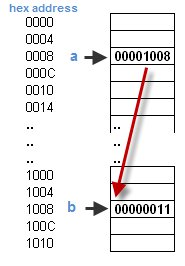
\includegraphics[scale=0.7]{images/pointeur.jpg}
\caption{Exemple, avec une variable a qui est un pointeur sur une
variable b}
\end{figure}

\subsection{Utilité des pointeurs}
\label{utilite-des-pointeurs}

Techniquement, il y a trois utilisations majeures des pointeurs en C :

\begin{itemize}
\item
  le passage de références à des fonctions ;
\item
  la manipulation de données complexes ;
\item
  l'allocation dynamique de mémoire.
\end{itemize}

\subsubsection{Passage de références à des fonctions}
\label{passage-de-references-a-des-fonctions}

Rappelez-vous du chapitre sur les fonctions : lorsque vous fournissez un
argument lors d'un appel, la valeur de celui-ci est affectée au
paramètre correspondant, paramètre qui est une variable propre à la
fonction appelée. Toutefois, il est parfois souhaitable de modifier une
variable de la fonction \emph{appelante}. Dès lors, plutôt que de passer
la valeur de la variable en argument, c'est une référence vers celle-ci
qui sera envoyée à la fonction.

\subsubsection{Manipulation de données complexes}
\label{manipulation-de-donnees-complexes}

Jusqu'à présent, nous avons manipulé des données simples : \mybox{int},
\mybox{double}, \mybox{char}, etc. Cependant, le C nous permet
également d'utiliser des données plus complexes qui sont en fait des
\textbf{agrégats} (un regroupement si vous préférez) de données simples.
Or, il n'est possible de manipuler ces agrégats qu'en les parcourant
données simples par données simples, ce qui requiert de disposer d'une
référence vers les données qui le composent.

\begin{infobox}
Nous verrons les agrégats plus en détails lorsque nous aborderons les
structures et les tableaux.
\end{infobox}


\subsection{L'allocation dynamique de mémoire}
\label{lallocation-dynamique-de-memoire}

Il n'est pas toujours possible de savoir quelle quantité de mémoire sera
utilisée par un programme. En effet, si vous prenez le cas d'un logiciel
de dessin, ce dernier ne peut pas prévoir quelle sera la taille des
images qu'il va devoir manipuler. Pour palier à ce problème, les
programmes recours au mécanisme de l'\textbf{allocation dynamique de
mémoire} : ils demandent de la mémoire au système d'exploitation lors de
leur exécution. Pour que cela fonctionne, le seul moyen est que le
système d'exploitation fournisse au programme une référence vers la zone
allouée.

\section{Déclaration et initialisation}
\label{declaration-et-initialisation-1}

La syntaxe pour déclarer un pointeur est la suivante.

\begin{C}
type *nom_du_pointeur;
\end{C}

Par exemple, si nous souhaitons créer un pointeur sur \mybox{int}
(c'est-à-dire un pointeur pouvant stocker l'adresse d'un objet de type
\mybox{int}) et que nous voulons le nommer « ptr », nous devons écrire
ceci.

\begin{C}
int *ptr;
\end{C}

L'astérisque peut être entourée d'espaces et placée n'importe où entre
le type et l'identificateur. Ainsi, les trois définitions suivantes sont
identiques.

\begin{C}
int *ptr;
int * ptr;
int* ptr;
\end{C}

\begin{attentionbox}
Notez bien qu'un pointeur est toujours typé. Autrement dit, vous aurez
toujours un pointeur sur (ou vers) un objet d'un certain type (\mybox{int},
\mybox{double}, \mybox{char}, etc.).
\end{attentionbox}

\subsection{Initialisation}
\label{initialisation-2}

Un pointeur, comme une variable, ne possède pas de valeur par défaut, il
est donc important de l'initialiser pour éviter d'éventuels problèmes.
Pour ce faire, il est nécessaire de recourir à l'\textbf{opérateur
d'adressage} (ou de référencement) : \mybox{\&} qui permet d'obtenir
l'adresse d'un objet. Ce dernier se place derrière l'objet dont
l'adresse souhaite être obtenue. Par exemple comme ceci.

\begin{C}
int a = 10;
int *p;

p = &a;
\end{C}

Ou, plus directement, comme cela.

\begin{C}
int a = 10;
int *p = &a;
\end{C}

\begin{erreurbox}
Faites bien attention à ne pas mélanger différents types de pointeurs !
Un pointeur sur \mybox{int} n'est pas le même qu'un pointeur sur \mybox{long}
ou qu'un pointeur sur \mybox{double}. De même, n'affectez l'adresse d'un
objet qu'à un pointeur du même type.
\begin{C}
 int a;
double b;
int *p = &b; /* faux */
int *q = &a; /* correct */
double *r = p; /* faux */
\end{C}
\end{erreurbox}

\subsection{Pointeur nul}
\label{pointeur-nul}

Vous souvenez-vous du chapitre sur la gestion d'erreur ? Dans ce
dernier, nous vous avons dit que, le plus souvent, les fonctions
retournaient une valeur particulière en cas d'erreur. \emph{Quid} de
celles qui retournent un pointeur ? Existe-t-il une valeur spéciale qui
puisse représenter une erreur ou bien sommes-nous condamner à utiliser
une variable globale comme \mybox{errno} ?

Heureusement pour nous, il existe un cas particulier : les pointeurs
nuls. Un pointeur nul est tout simplement un pointeur contenant une
adresse invalide. Cette adresse invalide dépend de votre système
d'exploitation, mais elle est la même pour tous les pointeurs nuls.
Ainsi, deux pointeurs nuls ont une valeur égale.

Pour obtenir cette adresse invalide, il vous suffit de convertir
explicitement zéro vers le type de pointeur voulu. Ainsi, le pointeur
suivant est un pointeur nul.

\begin{C}
int *p = (int *)0;
\end{C}

\begin{infobox}
Rappelez-vous qu'il y a conversion implicite vers le type de destination
dans le cas d'une affectation. La conversion est donc superflue dans ce cas-ci. 
\end{infobox}


\subsubsection{La constante NULL}
\label{la-constante-null}

Afin de clarifier un peu les codes sources, il existe une constante
définie dans l'en-tête \mybox{\textless{}stddef.h\textgreater{}} :
\mybox{NULL}. Celle-ci peut être utilisée partout où un pointeur nul
est attendu \emph{sauf comme argument de la fonction \mybox{printf()}}
(nous verrons pourquoi plus tard dans ce cours).

\begin{C}
int *p = NULL; /* Un pointeur nul. */
\end{C}

\section{Utilisation }
\label{utilisation-2}

\subsection{Indirection (ou déréférencement)}
\label{indirection-(ou déréférencement)}

Maintenant que nous savons récupérer l'adresse d'un objet et l'affecter
à un pointeur, voyons le plus intéressant : accéder à cet objet ou le
modifier via le pointeur. Pour y parvenir, nous avons besoin de
l'\textbf{opérateur d'indirection} (ou de déréférencement) : \mybox{*}.

\begin{questionbox}
 Le symbole \mybox{*} n'est pas celui de la multiplication ? 
\end{questionbox}

Si, c'est aussi le symbole de la multiplication. Toutefois, à l'inverse
de l'opérateur de multiplication, l'opérateur d'indirection ne prends
qu'un seul opérande (il n'y a donc pas de risque de confusion).

L'opérateur d'indirection attends un pointeur comme opérande et se place
juste derrière celui-ci. Une fois appliqué, ce dernier nous donne accès
à la valeur de l'objet référencé par le pointeur, aussi bien pour la
lire que pour la modifier.

Dans l'exemple ci-dessous, nous accédons à la valeur de la variable
\mybox{a} via le pointeur \mybox{p}.

\begin{C}
int a = 10;
int *p = &a;

printf("a = %d\n", *p);
\end{C}

\begin{C}
a = 10
\end{C}

À présent, modifions la variable \mybox{a} à l'aide du pointeur
\mybox{p}.

\begin{C}
int a = 10;
int *p = &a;

*p = 20;
printf("a = %d\n", *p);
\end{C}

\begin{C}
a = 20
\end{C}

\begin{infobox}
Comme pour n'importe quelle variable,
il est possible de déclarer un pointeur comme constant. Cependant,
puisqu'un pointeur référence un objet, il peut également être déclaré
comme un pointeur vers un objet constant. Pour ce faire, la position du
mot-clé \mybox{const} est importante. Si le
mot-clé est devant l'identificateur et derrière le symbole \mybox{*},
alors il s'agit d'un pointeur constant.
\begin{C}
int * const ptr; /* Un pointeur constant sur int. */
\end{C}

Si le mot-clé est devant le symbole \mybox{*} et derrière le type référencé, alors il s'agit d'un pointeur vers un objet
constant. 

\begin{C}
int const *ptr; /* Pointeur sur int constant. */
\end{C}

Enfin, ces deux notations peuvent être combinées
pour créer un pointeur constant vers un objet constant. 

\begin{C}
int const * const ptr; /* Pointeur constant sur int constant. */
\end{C}
\end{infobox}

\subsection{Passage comme argument}
\label{passage-comme-argument}

Voici un exemple de passage de pointeurs en arguments d'une fonction.

\begin{C}
#include <stdio.h>

void test(int *pa, int *pb)
{
    *pa = 10;
    *pb = 20;
}


int main(void)
{
    int a;
    int b;
    int *pa = &a;
    int *pb = &b;

    test(&a, &b);
    test(pa, pb);
    printf("a = %d, b = %d\n", a, b);
    printf("a = %d, b = %d\n", *pa, *pb);
    return 0;
}
\end{C}

\begin{C}
a = 10, b = 20
a = 10, b = 20
\end{C}

Remarquez que les appels \mybox{test(\&a,\ \&b)} et
\mybox{test(pa,\ pb)} réalisent la même opération.

\section{Retour de fonction}\label{retour-de-fonction}

Pour terminer, sachez qu'une fonction peut également retourner un
pointeur. Cependant, faites attention : \emph{l'objet référencé par le
pointeur doit toujours exister au moment de son utilisation} ! L'exemple
ci-dessous est donc incorrect étant donnée que la variable \mybox{n}
est de classe de stockage automatique et qu'elle n'existe donc plus
après l'appel à la fonction \mybox{ptr()}.

\begin{C}
#include <stdio.h>


int *ptr(void)
{
    int n;

    return &n;
}


int main(void)
{
    int *p = ptr();

    *p = 10;
    printf("%d\n", *p);
    return 0;
}
\end{C}

L'exemple devient correct si \mybox{n} est de classe de stockage
statique.

\section{Pointeur de pointeur}\label{pointeur-de-pointeur}

Au même titre que n'importe quel autre objet, un pointeur a lui aussi
une adresse. Dès lors, il est possible de créer un objet pointant sur ce
pointeur : un pointeur de pointeur.

\begin{C}
int a = 10;
int *pa = &a;
int **pp = &pa;
\end{C}

Celui-ci s'utilise de la même manière qu'un pointeur si ce n'est qu'il
est possible d'opérer deux indirections : une pour atteindre le pointeur
référencé et une seconde pour atteindre la variable sur laquelle pointe
le premier pointeur.

\begin{C}
#include <stdio.h>


int main(void)
{
    int a = 10;
    int *pa = &a;
    int **pp = &pa;

    printf("a = %d\n", **pp);
    return 0;
}
\end{C}

\begin{infobox}
Ceci peut continuer à l'infini pour concevoir 
des pointeurs de pointeur de pointeur de pointeur de\ldots{}
Bref, vous avez compris le principe.
\end{infobox}

\section{Pointeurs génériques et affichage}
\label{pointeurs-generiques-et-affichage}

\# Le type \mybox{void}

Vous avez déjà recontré le mot-clé \mybox{void} lorsque nous avons
parlé des fonctions, ce dernier permet d'indiquer qu'une fonction
n'utilise aucun paramètre et/ou ne retourne aucune valeur. Toutefois,
nous n'avons pas tout dit à son sujet : \mybox{void} est en fait un
type, au même titre que \mybox{int} ou \mybox{double}. o\_O

\begin{questionbox}
Et il représente quoi ce type, alors ?
\end{questionbox}


\emph{Hum}\ldots{} rien (d'où son nom). :-°\\
En fait, il s'agit d'un type dit « \textbf{incomplet} », c'est à dire
que la taille de ce dernier n'est pas calculable et qu'il n'est pas
utilisable dans des expressions. Quel est l'intérêt de la chose me
direz-vous ? Permettre de créer des pointeurs « \textbf{génériques} »
(ou « universels »).

En effet, nous venons de vous dire qu'un pointeur devait toujours être
typé. Cependant, cela peut devenir gênant si vous souhaitez créer une
fonction qui doit pouvoir travailler avec n'importe quel type de
pointeur (nous verrons un exemple très bientôt). C'est ici que le type
\mybox{void} intervient : un pointeur sur \mybox{void} est considéré
comme un pointeur générique, ce qui signifie qu'il peut référencer
n'importe quel type d'objet.

En conséquence, il est possible d'affecter n'importe quelle adresse
d'objet à un pointeur sur \mybox{void} et d'affecter un pointeur sur
\mybox{void} à n'importe quel autre pointeur (et inversément).

\begin{C}
int a;
double b;
void *p;
double *r;

p = &a; /* correct */
p = &b; /* correct */
r = p; /* correct */
\end{C}

\section{Afficher une adresse}\label{afficher-une-adresse}

Il est possible d'afficher une adresse à l'aide de l'indicateur de
conversion \mybox{p} de la fonction \mybox{printf()}. Ce dernier
attends en argument un pointeur sur \mybox{void}. Vous voyez ici
l'intérêt d'un pointeur générique : un seul indicateur suffit pour
afficher tous les types de pointeurs.

Notez que l'affichage s'effectue le plus souvent en hexadécimal.

\begin{C}
int a;
int *p = &a;

printf("%p == %p\n", (void *)&a, (void *)p);
\end{C}

Tant que nous y sommes, profitons en pour voir quelle est l'adresse
invalide de notre système.

\begin{C}
printf("%p\n", (void *)0);
\end{C}

\begin{secretbox}
Oui, le plus souvent, il s'agit de zéro. 
\end{secretbox}


\section{Exercice}
\label{exercice-12}


Pour le moment, tout ceci doit sans doute vous paraître quelques peu 
abstrait et sans doute inutile. Toutefois, rassurez-vous, cela vous semblera
plus clair après les chapitres suivants.

En attendant, nous vous proposons un petit exercice mettant en pratique
les pointeurs : programmez une fonction nommée « swap », dont le rôle
est d'échanger la valeur de deux variables de type \mybox{int}.
Autrement dit, la valeur de la variable « a » doit devenir celle de « b
» et la valeur de « b », celle de « a ».

\section{Correction}
\label{correction-14}

\begin{C}
 #include <stdio.h>

void swap(int *, int *);


void swap(int *pa, int *pb)
{
    int tmp;

    tmp = *pa;
    *pa = *pb;
    *pb = tmp;
}


int main(void)
{
    int a = 10;
    int b = 20;

    swap(&a, &b);
    printf("a = %d, b = %d\n", a, b);
    return 0;
}
\end{C}

\hrulefill

Nous en avons fini avec les pointeurs, du moins, pour le moment.

En effet, les pointeurs sont omniprésents en langage C et nous n'avons
pas fini d'en entendre parler. Mais pour l'heure, nous allons découvrir
une des fameuses données complexes dont nous avons parlé en début de
chapitre : les \textbf{structures}.
\chapter{Les structures}
\label{les-structures}

Dans le chapitre précédent, nous vous avions dit que
les pointeurs étaient entre autres utiles pour manipuler des données
complexes. Les structures sont les premières que nous allons étudier.

Une \textbf{structure} est un regroupement de plusieurs objets, de types
différents ou non. \emph{Grosso modo}, une structure est finalement une
boîte qui regroupe plein de données différentes.

\section{Définition, initialisation et utilisation}
\label{definition,-initialisation-et-utilisation}

\subsection{Définition d'une structure}
\label{definition-dune-structure}

Une structure étant un regroupement d'objets, la première chose à
réaliser est la description de celle-ci (techniquement, sa
\textbf{définition}), c'est-à-dire préciser de quel(s) objet(s) cette
dernière va se composer.

La syntaxe de toute définition est la suivante.

\begin{C}
struct étiquette
{
    /* Objet(s) composant(s) la structure. */
};
\end{C}

Prenons un exemple concret : vous souhaitez demander à l'utilisateur
deux mesures de temps sous la forme
heure(s):minute(s):seconde(s).milliseconde(s) et lui donner la
différence entre les deux en seconde. Vous pourriez utiliser six
variables pour stocker ce que vous fourni l'utilisateur, toutefois cela
reste assez lourd. À la place, nous pourrions représenter chaque mesure
à l'aide d'une structure composée de trois objets : un pour les heures,
un pour les minutes et un pour les secondes.

\begin{C}
struct temps {
    unsigned heures;
    unsigned minutes;
    double secondes;
};
\end{C}

Comme vous le voyez, nous avons donner un nom (plus précisémment, une
\textbf{étiquette}) à notre structure : « temps ». Les règles à
respecter sont les même que pour les noms de variable et de fonction.

Pour le reste, la composition de la structure est décrite à l'aide d'une
suite de déclarations de variable. Ces différentes déclarations
constituent les \textbf{membres} ou \textbf{champs} de la structure.
Notez bien qu'il s'agit de \emph{déclarations} et non de définitions,
l'utilisation d'initialisations est donc exclue.

Enfin, notez la présence d'un point-virgule \emph{obligatoire} à la fin
de la définition de la structure.

\begin{infobox}
Une structure ne peut pas comporter plus de cent vingt-sept membres. 
\end{infobox}


\subsection{Définition d'une variable de type structure}
\label{definition-dune-variable-de-type-structure}

Une fois notre structure décrite, il ne nous reste plus qu'à créer une
variable de ce type. Pour ce faire, la syntaxe est la suivante.

\begin{C}
struct étiquette identificateur;
\end{C}

La méthode est donc la même que pour définir n'importe quelle variable,
si ce n'est que le type de la variable est précisé à l'aide du mot-clé
\mybox{struct} et de l'étiquette de la structure. Avec notre exemple de
la structure \mybox{temps}, cela donne ceci.

\begin{C}
#include <stdio.h>

struct temps {
    unsigned heures;
    unsigned minutes;
    double secondes;
};


int main(void)
{
    struct temps t;

    return 0;
}
\end{C}

\subsection{Initialisation}
\label{initialisation-3}

Comme pour n'importe quelle autre variable, il est possible
d'initialiser une variable de type structure dès sa définition.
Toutefois, à l'inverse des autres, l'initialisation s'effectue à l'aide
d'une liste fournissant une valeur pour chaque membre de la structure.

L'exemple ci-dessous initialise le membre \mybox{heures} à 1,
\mybox{minutes} à 45 et \mybox{secondes} à 30.560.

\begin{C}
struct temps t = { 1, 45, 30.560 };
\end{C}

\begin{attentionbox}
Dans le cas où vous ne fournissez pas
un nombre suffisant de valeurs, les membres oubliés seront initialisés à
zéro ou, s'il s'agit de pointeurs, seront des pointeurs nuls. 
\end{attentionbox}


\subsection{Accès à un membre}
\label{acces-a-un-membre}

L'accès à un membre d'une structure se réalise à l'aide de la variable
de type structure et de l'opérateur \mybox{.} suivi du nom du champ
visé.

\begin{C}
variable.membre
\end{C}

Cette syntaxe peut être utilisée aussi bien pour obtenir la valeur d'un
champ que pour en modifier le contenu. L'exemple suivant effectue donc
la même action que l'initialisation présentée précédemment.

\begin{C}
t.heures = 1;
t.minutes = 45;
t.secondes = 30.560;
\end{C}

\subsection{Exercice}
\label{exercice-5}

Afin d'assimiler tout ceci, voici un petit exercice.\\
Essayez de réaliser ce qui a été décrit plus haut : demandez à
l'utilisateur de vous fournir deux mesures de temps sous la forme
heure(s):minute(s):seconde(s).milliseconde(s) et donnez lui la
différence en seconde entre celles-ci.

Voici un exemple d'utilisation.

\begin{C}
Première mesure (hh:mm:ss.xxx) : 12:45:50.640
Deuxième mesure (hh:mm:ss.xxx) : 13:30:35.480
Il y 2684.840 seconde(s) de différence.
\end{C}

\subsubsection{Correction}
\label{correction-15}

\begin{C}
#include <stdio.h>
#include <stdlib.h>

struct temps {
    unsigned heures;
    unsigned minutes;
    double secondes;
};



int main(void)
{
    struct temps t1;
    struct temps t2;

    printf("Première mesure (hh:mm:ss) : ");

    if (scanf("%u:%u:%lf", &t1.heures, &t1.minutes, &t1.secondes) != 3)
    {
        printf("Mauvaise saisie\n");
        return EXIT_FAILURE;
    }

    printf("Deuxième mesure (hh:mm:ss) : ");

    if (scanf("%u:%u:%lf", &t2.heures, &t2.minutes, &t2.secondes) != 3)
    {
        printf("Mauvaise saisie\n");
        return EXIT_FAILURE;
    }

    t1.minutes += t1.heures * 60;
    t1.secondes += t1.minutes * 60;
    t2.minutes += t2.heures * 60;
    t2.secondes += t2.minutes * 60;

    printf("Il y a %.3f seconde(s) de différence.\n",
    t2.secondes - t1.secondes);
    return 0;
}
\end{C}

\section{Structures et pointeurs}
\label{structures-et-pointeurs}

Certains d'entre vous s'en étaient peut-être doutés : s'il existe un 
objet d'un type, il doit être possible de créer un pointeur vers un
objet de ce type. Si oui, sachez que vous aviez raison. :)

\begin{C}
struct temps *p;
\end{C}

La définition ci-dessus créer un pointeur \mybox{p} vers un objet de
type \mybox{struct\ temps}.

\subsection{Accès via un pointeur}
\label{acces-via-un-pointeur}

L'utilisation d'un pointeur sur structure est un peu plus complexe que
celle d'un pointeur vers un type de base. En effet, il y a deux choses à
gérer : l'accès via le pointeur et l'accès à un membre. Intuitivement,
vous combineriez sans doute les opérateurs \mybox{*} et \mybox{.}
comme ceci.

\begin{C}
*p.heures = 1;
\end{C}

Toutefois, cette syntaxe ne correspond pas à ce que nous voulons car
l'opérateur \mybox{.} s'applique \emph{prioritairement} à l'opérateur
\mybox{*}. Autrement dit, le code ci-dessus accède au champ
\mybox{heures} et tente de lui appliquer l'opérateur d'indirection, ce
qui est incorrect puisque le membre \mybox{heures} est un entier non
signé.

Pour résoudre ce problème, nous devons utiliser des parenthèses afin que
l'opérateur \mybox{.} soit appliqué \emph{après} le déréférencement, ce
qui donne la syntaxe suivante.

\begin{C}
(*p).heures = 1;
\end{C}

Cette écriture étant un peu lourde, le C fourni un autre opérateur qui
combine ces deux opérations : l'opérateur \mybox{-\textgreater{}}.

\begin{C}
p->heures = 1;
\end{C}

Le code suivant initialise donc la structure \mybox{t} via le pointeur
\mybox{p}.

\begin{C}
struct temps t;
struct temps *p = &t;

p->heures = 1;
p->minutes = 45;
p->secondes = 30.560;

\end{C}

\subsection{Adressage}
\label{adressage}

Il est important de préciser que l'opérateur d'adressage peut
s'appliquer aussi bien à une structure qu'à un de ses membres. Ainsi,
dans l'exemple ci-dessous, nous définissons un pointeurs \mybox{p}
pointant sur la structure \mybox{t} et un pointeur \mybox{q} pointant
sur le champ \mybox{heures} de la structure \mybox{t}.

\begin{C}
struct temps t;
struct temps *p = &t;
int *q = &t.heures;
\end{C}

\subsection{Pointeurs sur structures et fonctions}
\label{pointeurs-sur-structures-et-fonctions}

Indiquons enfin que l'utilisation de pointeurs est particulièrement
propice dans le cas du passage de structures à des fonctions. En effet,
rappelez-vous, lorsque vous fournissez un argument lors d'un appel de
fonction, la valeur de celui-ci est affectée au paramètre correspondant.
Cette règle s'applique également aux structures : la valeur de chacun
des membres est copiée une à une. Dès lors, si la structure passée en
argument comporte beaucoup de champs, la copie risque d'être longue.
L'utilisation d'un pointeur évite ce problème puisque seule la valeur du
pointeur (autrement dit, l'adresse vers la structure) sera copiée et non
toute la structure.

\section{Portée et déclarations}
\label{portee-et-declarations}

Dans les exemples précédents, nous avons toujours placés notre
définition de structure en dehors de toute fonction. Cependant, sachez
que celle-ci peut être circonscrite à un bloc de sorte de limiter sa
\textbf{portée}, comme pour les définitions de variables et les
déclarations de variables et fonctions.

Dans l'exemple ci-dessous, la structure \mybox{temps} ne peut être
utilisée que dans le bloc de la fonction \mybox{main()} et les
éventuels sous-blocs qui la composent.

\begin{C}
int main(void)
{
    struct temps {
        unsigned heures;
        unsigned minutes;
        double secondes;
    };

    struct temps t;

    return 0;
}
\end{C}

Notez qu'il est possible de combiner une définition de structure et une
définition de variable. En effet, une définition de structure n'étant
rien d'autre que la définition d'un nouveau type, celle-ci peut être
placée là où est attendu un type dans une définition de variable. Avec
l'exemple précédent, cela donne ceci.

\begin{C}
int main(void)
{
    struct temps {
        unsigned heures;
        unsigned minutes;
        double secondes;
    } t1;
    struct temps t2;

    return 0;
}
\end{C}

Il y a trois définitions dans ce code : celle du type
\mybox{struct\ temps} , celle de la variable \mybox{t1} et celle de la
variable \mybox{t2}. Après sa définition, le type
\mybox{struct\ temps} peut tout à fait être utilisé pour définir
d'autres variables de ce type, ce qui est le cas de \mybox{t2}.

\begin{infobox}
 Notez qu'il est possible de condenser
la définition du type \mybox{struct\ temps} et de la variable
\mybox{t1} sur une seule ligne, comme ceci.
\begin{C}
 struct temps { unsigned heures; unsigned minutes; double secondes; } t1;
\end{C}
\end{infobox}


S'agissant d'une définition de variable, il est également parfaitement
possible de l'initialiser.

\begin{C}
int main(void)
{
    struct temps {
        unsigned heures;
        unsigned minutes;
        double secondes;
    } t1 = { 1, 45, 30.560 };
    struct temps t2;

    return 0;
}
\end{C}

Enfin, précisions que l'étiquette d'une structure peut être omise lors
de sa définition. Néanmoins, cela ne peut avoir lieu que si la
définition de la structure est combinée avec une définition de variable.
C'est assez logique étant donné qu'il ne peut pas être fait référence à
cette définition à l'aide d'une étiquette.

\begin{C}
int main(void)
{
    struct {
        unsigned heures;
        unsigned minutes;
        double secondes;
    } t;

    return 0;
}
\end{C}

\subsection{Déclarations}
\label{declarations}

Jusqu'à présent, nous avons parlé de définitions de structures,
toutefois, comme pour les variables et les fonctions, il existe
également des déclarations de structures. Une déclaration de structure
est en fait une définition sans le corps de la structure.

\begin{C}
struct temps;
\end{C}

Quel est l'intérêt de la chose me direz-vous ? Résoudre deux types de
problèmes : les structures interdépendantes et les structures comportant
un ou des membres qui sont des pointeurs vers elle-même.

\subsection{Les structures interdépendantes}
\label{les-structures-interdependantes}

Deux structures sont interdépendantes lorsque l'une comprend un pointeur
vers l'autre et inversément.

\begin{C}
struct a {
    struct b *p;
};

struct b {
    struct a *p;
};
\end{C}

Voyez-vous le problème ? Si le type \mybox{struct\ b} ne peut être
utilisé qu'après sa définition, alors le code ci-dessus est faux et le
cas de structures interdépendantes est insoluble. Heureusement, il est
possible de \textbf{déclarer} le type \mybox{struct\ b} afin de pouvoir
l'utiliser \emph{avant} sa définition.

\begin{erreurbox}
Une déclaration de structure crée un type dit \textbf{incomplet}
(comme le type \mybox{void}). Dès lors, il ne peut pas être 
utilisé pour définir une variable (puisque les membres qui composent
la structure sont inconnus). Ceci n'est utilisable que pour
définir des pointeurs.
\end{erreurbox}


Le code ci-dessous résoud le « problème » en déclarant le type
\mybox{struct\ b} avant son utilisation.

\begin{C}
struct b;

struct a {
    struct b *p;
};

struct b {
    struct a *p;
};
\end{C}

Nous avons entouré le mot « problème » de guillemets car le premier code
que nous vous avons montré n'en pose en fait aucun et compile sans
sourciller. :-°

En fait, afin d'éviter ce genre d'écritures, le langage C prévoit
l'ajout de \textbf{déclarations implicites}. Ainsi, lorsque le
compilateur recontre un pointeur vers un type de structure qu'il ne
connaît pas, il ajoute implicitement une déclaration de cette structure
juste avant. Ainsi, le premier et le deuxième code sont équivalents si
ce n'est que le premier comporte une déclaration implicite et non une
déclaration explicite.

\subsection{Structure qui pointe sur elle-même}
\label{structure-qui-pointe-sur-elle-meme}

Le deuxième cas où les déclarations de structure s'avèrent nécessaires
est celui d'une structure qui comporte un pointeur vers elle-même.

\begin{C}
struct a {
    struct a *p;
};
\end{C}

De nouveau, si le type \mybox{struct\ a} n'est utilisable qu'après sa
définition, c'est grillé. Toutefois, comme pour l'exemple précédent, le
code est correct, mais pas tout à fait pour les même raisons. Dans ce
cas ci, le type \mybox{struct\ a} est connu car nous sommes en train de
le définir. Techniquement, dès que la définition commence, le type est
déclaré.

\begin{infobox}
Notez que, comme les définitions, les déclarations (implicites ou non)
ont une portée.
\end{infobox}

\section{Un peu de mémoire}
\label{un-peu-de-memoire}

Savez-vous comment sont représentées les structures en
mémoire ?

Les membres d'une structure sont placés les uns après les autres en
mémoire. Par exemple, prenons cette structure.

\begin{C}
 struct exemple
{
    double flottant;
    char lettre;
    unsigned entier;
};
\end{C}

Si nous supposons qu'un \mybox{double} a une taille de huit octets, un
\mybox{char} de un octet, et un \mybox{unsigned\ int} de quatre
octets, voici ce que devrait donner cette structure en mémoire.

\begin{figure}[htbp]
\centering
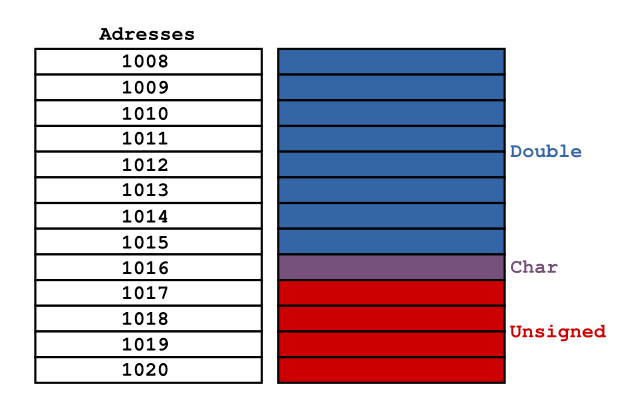
\includegraphics[scale=0.5]{images/structure_memoire.png}
\caption{Représentation en mémoire de la structure}
\end{figure}

\begin{infobox}
Les adresses spécifiées dans le schéma sont fictives et 
ne servent qu'à titre d'illustration.
\end{infobox}


\subsection{L'opérateur sizeof}
\label{loperateur-sizeof}

Voyons à présent comment déterminer cela de manière plus précise, en
commençant par la taille des types. L'opérateur \mybox{sizeof} permet
de connaître la taille en multiplets (\emph{bytes} en anglais) de son
opérande. Cet opérande peut être soit un type (qui doit alors être entre
parenthèses), soit une expression (auquel cas les parenthèses sont
facultatives).

Le résultat de cet opérateur est de type \mybox{size\_t}. Il s'agit
d'un type entier \emph{non signé} défini dans l'en-tête
\mybox{\textless{}stddef.h\textgreater{}} qui est capable de contenir
la taille de n'importe quel objet. L'exemple ci-dessous utilise
l'opérateur \mybox{sizeof} pour obtenir la taille des types de bases.

\begin{C}
#include <stddef.h>
#include <stdio.h>


int main(void)
{
    double f;

    printf("char: %u\n", (unsigned)sizeof(char));
    printf("short: %u\n", (unsigned)sizeof(short));
    printf("int : %u\n", (unsigned)sizeof(int));
    printf("long : %u\n", (unsigned)sizeof(long));
    printf("float : %u\n", (unsigned)sizeof(float));
    printf("double : %u\n", (unsigned)sizeof(double));
    printf("long double : %u\n", (unsigned)sizeof(long double));

    printf("int : %u\n", (unsigned)sizeof 5);
    printf("double : %u\n", (unsigned)sizeof f);
    return 0;
}
\end{C}

\begin{C}
char : 1
short : 2
int : 4
long : 8
float : 4
double : 8
long double : 16
int : 4
double : 8
\end{C}

\begin{infobox}
Le type \mybox{char} a \emph{toujours} une taille de un multiplet.
\end{infobox}


Malheureusement pour nous, la fonction \mybox{printf()} ne fournit pas
d'indicateur de conversion pour le type \mybox{size\_t}\footnote{Depuis
la norme C99, il existe un indicateur de conversion \mybox{zu} qui
permet d'afficher une expression de type \mybox{size\_t}.}. Dès lors,
nous devons recourir à une conversion explicite afin de pouvoir utiliser
un autre indicateur. En l'occurrence, nous avons choisi le type
\mybox{unsigned\ int} étant donné que la taille des types de base est
très petite et qu'il n'y a en conséquence pas de risque de dépasser sa
capacité.

Remarquez que les parenthèses ne sont pas obligatoires dans le cas où
l'opérande de l'opérateur \mybox{sizeof} est une expression (dans notre
exemple : 5 et \mybox{f}).

\begin{infobox}
 Il est parfaitement possible que vous n'obteniez pas les même valeurs que nous,
celles-ci dépendent de votre machine.
\end{infobox}


Ceci étant fait, voyons à présent ce que donne la taille de la structure
présentée plus haut. En toute logique, elle devrait être égale à la
somme des tailles de ses membres, chez nous : 13 (8 + 1 + 4).

\begin{C}
#include <stddef.h>
#include <stdio.h>

struct exemple
{
    double flottant;
    char lettre;
    unsigned int entier;
};


int main(void)
{
    printf("struct exemple : %u\n", (unsigned)sizeof(struct exemple));
    return 0;
}
\end{C}

\begin{C}
struct exemple : 16
\end{C}

\emph{Ah} ! Il semble que nous avons loupé quelque chose\ldots{} :-°

Pourquoi obtenons nous seize et non treize, comme attendu ? Pour
répondre à cette question, nous allons devoir plonger un peu dans les
entrailles de notre machine.

\subsection{Alignement en mémoire}
\label{alignement-en-memoire}

Le processeur et la mémoire vive communiquent entre eux à l'aide d'un
canal appelé un \textbf{bus mémoire}. Les communications à travers le
bus mémoire s'opèrent à l'initiative du processeur qui dispose
d'instructions spécifiques pour déplacer des données de la mémoire vers
un registre et inversement. Ce canal dispose d'une capacité de transport
limitée et ne peut en conséquence transmettre qu'un nombre fixé de
multiplets.

Toutefois, bien que la mémoire vive soit composée de multiplets, le
processeur utilise \emph{toujours} la capacité maximale du bus et lit ou
écrit dans celle-ci par blocs de la taille du bus. Dès lors, le
processeur ne va pas voir la mémoire vive comme une suite de multiplets,
mais comme une suite de blocs de la taille du bus qui sont le plus
souvent appelés des \textbf{mots}.

Quel rapport avec notre structure me direz-vous ? Supposons que notre
processeur lise des blocs de quatre octets à la fois. Si notre structure
faisait treize octets, voici comment le processeur la verrai.

\begin{figure}[htbp]
\centering
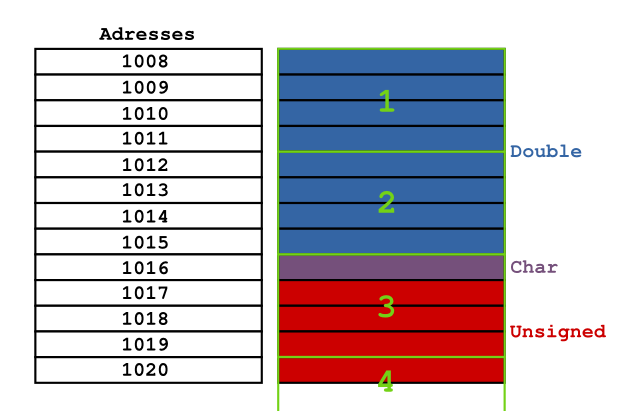
\includegraphics[scale=0.5]{images/vue_memoire_proc.png}
\caption{Vue de la mémoire par le processeur}
\end{figure}

Le premier champ est réparti sur plusieurs mots et remplit complètement
ces mots. Cette situation ne pose pas de problèmes : soit le processeur
charge la donnée en plusieurs fois (ce que la plupart des processeurs
savent faire automatiquement), soit le compilateur prévoit plusieurs
instructions de chargements.

Par contre, le membre de type \mybox{unsigned\ int} est problématique :
vu que sa taille est égale à celle d'un mot, son transfert devrait être
réalisé en une seule fois. Toutefois, dans notre exemple, le membre est
à califourchon sur deux mots. De ce fait, pour obtenir sa valeur, le
processeur devrait :

\begin{itemize}
\item
  charger le troisième mot et en extraire les bons octets ;
\item
  charger le quatrième mot et en extraire le bon octet ;
\item
  et, enfin, combiner le tout pour obtenir la valeur correcte.
\end{itemize}

C'est plus lent, sans compter que quelques rares processeurs ne gèrent
pas ce genre d'opérations et se contentent de signaler une erreur.

\begin{questionbox}
Mais, comment le processeur sait-il que le dernier champ est à cheval sur deux mots ?
\end{questionbox}


À cause de son adresse. Dans notre exemple, le membre de type
\mybox{unsigned\ int} est situé à l'adresse 1017. Étant donné qu'un
\mybox{unsigned\ int} a une taille de quatre octets et que le
processeur lit des mots de quatre octets, il sait que si une donnée de
ce type n'est pas à une adresse multiple de quatre, alors elle est
forcément à califourchon sur deux mots.

Pour éviter ces problèmes, les compilateurs ajoutent des multiplets dit
« de bourrage » (\emph{padding} en anglais), afin d'\textbf{aligner} les
données sur les bonnes adresses. Dans le cas de notre structure, le
compilateur a ajouté trois octets de bourrage juste après le membre de
type \mybox{char} afin que le dernier champ soit forcément à une
adresse multiple de quatre.

\begin{figure}[htbp]
\centering
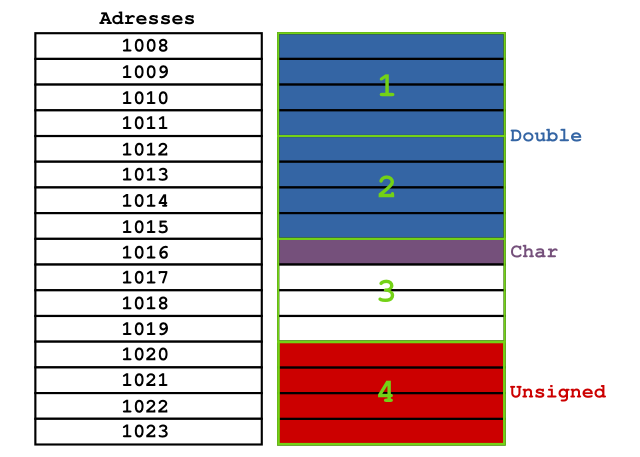
\includegraphics[scale=0.5]{images/structure_correct_align.png}
\caption{La structure correctement alignée}
\end{figure}

\subsection{La macrofonction offsetof}
\label{la-macrofonction-offsetof}

Il vous est possible de connaître les \textbf{contraintes d'alignement}
d'un type (c'est-à-dire le nombre dont doivent être multiple les
adresses d'un type) à l'aide de la \textbf{macrofonction}
\mybox{offsetof()}\footnote{\footnotesize{La norme C11 a introduit un nouvel
  opérateur \mybox{\_Alignof} (et un synonyme \mybox{alignof} fournit
  par l'en-tête \mybox{\textless{}stdalign.h\textgreater{}}) qui donne
  les contraintes d'alignement du type de son opérande. Il s'utilise de
  la même manière que l'opérateur \mybox{sizeof} et retourne lui aussi
  une valeur entière de type \mybox{size\_t}.}} qui est définie dans l'en-tête
\mybox{\textless{}stddef.h\textgreater{}} (nous verrons plus tard ce
qu'est une macrofonction lorsque nous aborderons le préprocesseur).
Cette dernière attends deux arguments : une définition de structure ou
un type de structure et le nom d'un membre de celle-ci. Elle retourne le
nombre de multiplets qui précède ce champ au sein de la structure. Son
retour est de type \mybox{size\_t}, comme pour l'opérateur
\mybox{sizeof}.

Étant donné que le type \mybox{char} prends un multiplet, si le premier
champ d'une structure est de ce type alors le membre suivant sera
forcément précédé du nombre de multiplets de bourrage nécessaire pour
qu'il soit bien aligné. Ainsi, le code suivant vous donne les
contraintes d'alignement pour chaque type de base.

\begin{C}
#include <stddef.h>
#include <stdio.h>


int main(void)
{
    printf("short: %u\n", (unsigned)offsetof(struct { char c; short n; }, n));
    printf("int : %u\n", (unsigned)offsetof(struct { char c; int n; }, n));
    printf("long : %u\n", (unsigned)offsetof(struct { char c; long n; }, n));
    printf("float : %u\n", (unsigned)offsetof(struct { char c; float f; }, f));
    printf("double : %u\n", (unsigned)offsetof(struct { char c; double f; }, f));
    printf("long double : %u\n", (unsigned)offsetof(struct { char c; long double f; }, f));
    return 0;
}
\end{C}

\begin{C}
short: 2
int : 4
long : 8
float : 4
double : 8
long double : 16
\end{C}

\begin{infobox}
Le type \mybox{char} ayant une taille de un multiplet, il peut 
\emph{toujours} être contenu dans un mot. Il n'a donc pas de 
contraintes d'alignement.
\end{infobox}


Pour chaque type, nous définissons une structure composée d'un premier
membre de type \mybox{char} et d'un second membre d'un type dont nous
souhaitons connaître les contraintes d'alignement. Cette définition est
utilisée comme premier argument de la macrofonction \mybox{offsetof()},
le deuxième étant le nom du second membre de la structure. Pour le
reste, le nombre retourné étant de type \mybox{size\_t}, nous opérons à
nouveau une conversion vers le type \mybox{unsigned\ int}.

\hrulefill

Les structures en elles-même ne sont pas compliquées à comprendre, mais 
l'intérêt est   parfois plus difficile à saisir. Ne vous en faîtes pas,
nous aurons bientôt l'occasion de découvrir des cas où les structures se
trouvent être bien pratiques. En attendant, n'hésitez pas à relire le 
chapitre s'il vous reste des points obscurs.

Continuons notre route et découvrons à présent un deuxième type de
données complexes : les \textbf{tableaux}.
\chapter{Les tableaux}
\label{les-tableaux}

Poursuivons notre tour d'horizon des données complexes avec
les \textbf{tableaux}.

Comme les structures, les tableaux sont des regoupements de plusieurs
objets. Cependant, à l'inverse de celles-ci, les tableaux regroupe des
données de \emph{même type} et de manière \emph{contiguë} (ce qui exclut
la présence de multiplets de bourrage).

\begin{figure}[htbp]
\centering
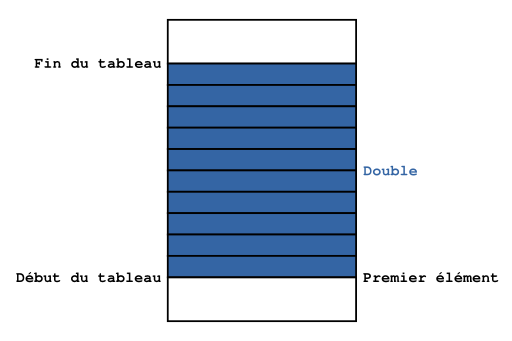
\includegraphics[scale=0.5]{images/tableau_memoire.png}
\caption{Représentation d'un tableau en mémoire}
\end{figure}

Un tableau est donc un gros bloc de mémoire de \emph{taille finie} qui
commence à une adresse déterminée : celle de son premier élément.

\section{Les tableaux simples (à une dimension)}
\label{les-tableaux-simples-(a-une-dimension}

\subsection{Définition}
\label{definition-1}

La définition d'un tableau nécessite trois informations :

\begin{itemize}
\item
  le type des éléments du tableau (rappelez-vous : un tableau est une
  suite de données de \emph{même type}) ;\\
\item
  le nom du tableau (en d'autres mots, son identificateur) ;\\
\item
  \textbf{la longueur} du tableau (le nombre d'éléments qui le
  composent). Cette dernière doit \emph{obligatoirement} être une
  constante entière.
\end{itemize}

\begin{C}
type identificateur[longueur];
\end{C}

Comme vous le voyez, la syntaxe de la déclaration d'un tableau est
similaire à celle d'une variable, la seule différence étant qu'il vous
est nécessaire de préciser le nombre d'éléments entre crochets à la
suite de l'identificateur du tableau.

Ainsi, si nous souhaitons par exemple définir un tableau contenant vingt
\mybox{int}, nous devons procéder comme suit.

\begin{C}
int tab[20];
\end{C}

\subsection{Initialisation}
\label{initialisation-4}

Comme pour les variables, il est possible d'initialiser un tableau ou,
plus précisément, tout ou partie de ses éléments.

\subsubsection{Initialisation avec une longueur explicite}
\label{initialisation-avec-une-longueur-explicite-1}

L'initialisation se réalise de la même manière que pour les structures,
c'est-à-dire à l'aide d'une liste d'initialisation.

\begin{C}
int tab[3] = { 1, 2, 3 };
\end{C}

L'exemple ci-dessus initialise les trois membres du tableau avec les
valeurs 1, 2 et 3.

\begin{attentionbox}
  Comme pour les structures, dans le cas
où vous ne fournissez pas un nombre suffisant de valeurs, les éléments
oubliés seront initialisés à zéro ou, s'il s'agit de pointeurs, seront
des pointeurs nuls.
\end{attentionbox}


Pour un tableau de structures, la liste d'initialisation comportera
elle-même une liste d'initialistation pour chaque structure composant le
tableau.

\begin{C}
struct temps tab[2] = { { 12, 45, 50.6401 }, { 13, 30, 35.480 } } ;
\end{C}

\begin{infobox}
 Notez que, inversément, une structure
peut comporter des tableaux comme membres.
\end{infobox}


\subsubsection{Initialisation avec une longueur implicite}
\label{initialisation-avec-une-longueur-implicite-1}

Lorsque vous initialisez un tableau, il vous est permis d'omettre la
longueur de celui-ci, car le compilateur sera capable d'en déterminer la
taille en comptant le nombre d'éléments présents dans la liste
d'initialisation. Ainsi, l'exemple ci-dessous est correct et défini un
tableau de trois \mybox{int} valant respectivement 1, 2 et 3.

\begin{C}
int tab[] = { 1, 2, 3 };
\end{C}

\subsection{Accès aux éléments d'un tableau}
\label{acces-aux-elements-dun-tableau}

L'accès aux éléments d'un tableau se réalise à l'aide d'un
\textbf{indice}, un nombre entier correspondant à la position de chaque
élément dans le tableau (premier, deuxième, troisième, etc). Cependant,
il y a une petite subtilité : \emph{les indices commencent toujours à
zéro}.

Ceci tient au fait que l'accès aux différents éléments est réalisé à
l'aide de l'adresse du premier élément à laquelle est ajouté l'indice
(qui doit donc être nul pour conserver l'adresse du premier élément).
Étant donné que tous les éléments ont la même taille et se suivent en
mémoire, leurs adresses peuvent effectivement se calculer à l'aide de
l'adresse du premier élément et d'un décalage par rapport à celle-ci
(l'indice, donc).

Prenons un exemple avec un tableau composés de \mybox{int} (ayant une
taille de quatre octets) et dont le premier élément est placé à
l'adresse 1008. Si vous déterminez à la main les adresses de chaque
élèment, vous obtiendrez ceci.

\begin{table}
\centering
\rowcolors{1}{gris-clair-tab}{}
\begin{tabular}{|l|l|}\hline
\rowcolor{gris-tab-entete}\textbf{\makecell{Indice}} & A\textbf{\makecell{dresse de l'élément}}\tabularnewline\hline
0 & 1008 (1008 + 0)\tabularnewline\hline
1 & 1012 (1008 + 4)\tabularnewline\hline
2 & 1016 (1008 + 8)\tabularnewline\hline
3 & 1020 (1008 + 12)\tabularnewline\hline
4 & 1024 (1008 + 16)\tabularnewline\hline
5 & 1028 (1008 + 20)\tabularnewline\hline
\ldots{} & \ldots{}\tabularnewline\hline
\end{tabular}
\end{table}

En fait, il est possible de reformuler ceci à l'aide d'une
multiplication entre l'indice et la taille d'un \mybox{int}.

\begin{table}
\centering
\rowcolors{1}{gris-clair-tab}{}
\begin{tabular}{|l|l|}\hline
\rowcolor{gris-tab-entete}\textbf{\makecell{Indice}} & \textbf{\makecell{Adresse de l'élément}}\tabularnewline\hline
0 & 1008 (1008 + (0 * 4))\tabularnewline\hline
1 & 1012 (1008 + (1 * 4))\tabularnewline\hline
2 & 1016 (1008 + (2 * 4))\tabularnewline\hline
3 & 1020 (1008 + (3 * 4))\tabularnewline\hline
4 & 1024 (1008 + (4 * 4))\tabularnewline\hline
5 & 1028 (1008 + (5 * 4))\tabularnewline\hline
\ldots{} & \ldots{}\tabularnewline\hline
\end{tabular}
\end{table}

Nous pouvons désormais formaliser mathématiquement tout ceci en posant
\(T\) la taille d'un élément du tableau, \(i\) l'indice de cet élément,
et \(A\) l'adresse de début du tableau (l'adresse du premier élément,
donc). L'adresse de l'élément d'indice \(i\) s'obtient en calculant
\(A + T \times i\). Ceci étant posé, voyons à présent comment mettre
tout cela en œuvre en C.

\subsubsection{Le premier élément}
\label{le-premier-element}

Pour commencer, nous avons besoin de l'adresse du premier élément du
tableau. Celle-ci s'obtient en fait d'une manière plutôt
contre-intuitive : lorsque vous utilisez une variable de type tableau
dans une expression, celle-ci est convertie implicitement en un pointeur
\emph{constant} sur son premier élément. Comme vous pouvez le constater
dans l'exemple qui suit, nous pouvons utiliser la variable \mybox{tab}
comme nous l'aurions fait s'il s'agissait d'un pointeur.

\begin{C}
#include <stdio.h>

int main(void)
{
    int tab[3] = { 1, 2, 3 };

    printf("Premier élément : %d\n", *tab);
    return 0;
}
\end{C}

\begin{C}
Premier élément : 1
\end{C}

Notez que comme il s'agit d'une conversion implicite vers un pointeur
constant, il n'est pas possible d'affecter une valeur à une variable de
type tableau. Ainsi, le code suivant est incorrect.

\begin{C}
int t1[3];
int t2[3];

t1 = t2; /* Incorrect. */
\end{C}

La règle de conversion implicite comprends néanmoins deux exceptions :
l'opérateur \mybox{\&} et l'opérateur \mybox{sizeof}.

Lorsqu'il est appliqué à une variable de type tableau, l'opérateur
\mybox{\&} produit comme résultat l'adresse du premier élément du
tableau. Si vous exécutez le code ci-dessous, vous constaterez que les
deux expressions donnent un résultat identique.

\begin{C}
#include <stdio.h>


int main(void)
{
    int tab[3];

    printf("%p == %p\n", (void *)tab, (void *)&tab);
    return 0;
}
\end{C}

Dans le cas où une expression de type tableau est fournie comme opérande
de l'opérateur \mybox{sizeof}, le résultat de celui-ci sera bien la
taille totale du tableau (en multiplets) et non la taille d'un pointeur.

\begin{C}
 #include <stdio.h>


int main(void)
{
    int tab[3];
    int *ptr;

    printf("sizeof tab = %u\n", (unsigned)sizeof tab);
    printf("sizeof ptr = %u\n", (unsigned)sizeof ptr);
    return 0;
}
\end{C}



\begin{C}
sizeof tab = 12
sizeof ptr = 8
\end{C}

Cette propriété vous permet d'obtenir le nombre d'éléments d'un tableau
à l'aide de l'expression suivante.

\begin{C}
sizeof tab / sizeof tab[0]
\end{C}

\subsubsection{Les autres éléments}
\label{les-autres-elements}

Pour accéder aux autres éléments, il va nous falloir ajouter la position
de l'élément voulu à l'adresse du premier élément et ensuite utiliser
l'adresse obtenue. Toutefois, recourir à la formule présentée au-dessus
ne marchera pas car, en C, les pointeurs sont typés. Dès lors, lorsque
vous additionnez un nombre à un pointeur, le compilateur multiplie
automatiquement ce nombre par la taille du type d'objet référencé par le
pointeur. Ainsi, pour un tableau de \mybox{int}, l'expression
\mybox{tab\ +\ 1} est implicitement convertie en
\mybox{tab\ +\ sizeof(int)}.

Voici un exemple affichant la valeur de tous les éléments d'un tableau.

\begin{C}
#include <stdio.h>


int main(void)
{
    int tab[3] = { 1, 2, 3 };

    printf("Premier élément : %d\n", *tab);
    printf("Deuxième élément : %d\n", *(tab + 1));
    printf("Troisième élément : %d\n", *(tab + 2));
    return 0;
}
\end{C}

\begin{C}
Premier élément : 1
Deuxième élément : 2
Troisième élément : 3
\end{C}

L'expression \mybox{*(tab\ +\ i)} étant quelque peu lourde, il existe
un opérateur plus concis pour réaliser cette opération : l'opérateur
\mybox{{[}{]}}. Celui-ci s'utilise de cette manière.

\begin{C}
expression[indice]
\end{C}

Ce qui est équivalent à l'expression suivante.

\begin{C}
*(expression + indice)
\end{C}

L'exemple suivant est donc identique au précédent.

\begin{C}
#include <stdio.h>


int main(void)
{
    int tab[3] = { 1, 2, 3 };

    printf("Premier élément : %d\n", tab[0]);
    printf("Deuxième élément : %d\n", tab[1]);
    printf("Troisième élément : %d\n", tab[2]);
    return 0;
}
\end{C}

\subsection{Parcours et débordement}
\label{parcours-et-debordement}

Une des erreurs les plus fréquente en C consiste à dépasser la taille
d'un tableau, ce qui est appelé un cas de \textbf{débordement}
(\emph{overflow} en anglais). En effet, si vous tentez d'accéder à un
objet qui ne fait pas partie de votre tableau, vous réalisez un accès
mémoire non autorisé, ce qui provoquera un comportement indéfini. Cela
arrive généralement lors d'un parcours de tableau à l'aide d'une boucle.

\begin{C}
#include <stdio.h>


int main(void)
{
    int tableau[5] = {784, 5, 45, -12001, 8};
    int somme = 0;
    unsigned i; 

    for (i = 0; i <= 5; ++i)
        somme += tableau[i];

    printf("%d\n", somme);
    return 0;
}
\end{C}

Le code ci-dessus est volontairement erroné et tente d'accéder à un
élément qui se situe au-delà du tableau. Ceci provient de l'utilisation
de l'opérateur \mybox{\textless{}=} à la place de l'opérateur
\mybox{\textless{}} ce qui entraîne un tour de boucle avec \mybox{i}
qui est égal à 5, alors que le dernier indice du tableau doit être
quatre.

\begin{attentionbox}
  N'oubliez pas : les indices d'un
tableau commencent \emph{toujours} à zéro. En conséquence, les indices
valides d'un tableau de \(n\) éléments vont de 0 à \(n-1\).
\end{attentionbox}


\subsection{Tableaux et fonctions}
\label{tableaux-et-fonctions}

\subsubsection{Passage en argument}
\label{passage-en-argument-1}

Étant donné qu'un tableau peut être utilisé comme un pointeur sur son
premier élément, lorsque vous passer un tableau en argument d'une
fonction, celle-ci reçoit un pointeur vers le premier élément du
tableau. Le plus souvent, il vous sera nécessaire de passer également la
taille du tableau afin de pouvoir le parcourir.

Le code suivante utilise une fonction pour parcourir un tableau d'entier
et afficher la valeur de chacun de ses éléments.

\begin{C}
#include <stdio.h>


void affiche_tableau(int *tab, unsigned taille)
{
    unsigned i;

    for (i = 0; i < taille; ++i)
        printf("tab[%u] = %d\n", i, tab[i]);
}


int main(void)
{
    int tab[5] = { 2, 45, 67, 89, 123 };

    affiche_tableau(tab, 5);
    return 0;
}
\end{C}

\begin{C}
tab[0] = 2
tab[1] = 45
tab[2] = 67
tab[3] = 89
tab[4] = 123
\end{C}

\begin{infobox}
Notez qu'il existe une syntaxe
alternative pour déclarer un paramètre de type tableau héritée du
langage B (voyez la dernière section)

\begin{C}
 void affiche_tableau(int tab[], unsigned taille)
\end{C}

Toutefois, nous vous conseillons de recourir à la
première écriture, cette dernière étant plus explicite.
\end{infobox}

\subsubsection{Retour de fonction}
\label{retour-de-fonction-1}

De la même manière que pour le passage en argument, retourner un tableau
revient à retourner un pointeur sur le premier élément de celui-ci.
Toutefois, n'oubliez pas les problématiques de classe de stockage ! Si
vous retournez un tableau de classe de stockage automatique, vous
fournissez à la fonction appelante un pointeur vers un objet qui
n'existe plus (puisque l'exécution de la fonction appelée est terminée).

\begin{C}
 #include <stdio.h>


int *tableau(void)
{
    int tab[5] = { 1, 2, 3, 4, 5 };

    return tab;
}


int main(void)
{
    int *p = tableau(); /* Incorrect. */

    printf("%d\n", p[0]);
    return 0;
}
\end{C}

\section{La vérité sur les tableaux }
\label{la-verite-sur-les-tableaux }

Nous vous avons dit qu'une variable de type tableau pouvait être
utilisée comme un pointeur constant sur son premier élément. Cependant,
ce n'est pas tout à fait vrai.

\subsection{Un peu d'histoire}
\label{un-peu-dhistoire}

Le prédécesseur du langage C était le langage B. Lorsque le
développement du C a commencé, un des objectifs était de le rendre
autant que possible compatible avec le B, afin de ne pas devoir (trop)
modifier les codes existants (un code écrit en B pourrait ainsi être
compilé avec un compilateur C sans ou avec peu de modifications). Or, en
B, un tableau se définissait comme suit.

\begin{C}
auto tab[3];
\end{C}

\begin{infobox}
Le langage B était un langage non
typé, ce qui explique l'absence de type dans la définition. Le mot-clé
\mybox{auto} (toujours présent en langage C, mais devenu obsolète)
servait à indiquer que la variable définie était de classe de stockage
automatique.
\end{infobox}


Toutefois, à la différence du langage C, cette définition créée un
tableau de trois éléments \emph{et} un pointeur initialisé avec
l'adresse du premier élément. Ainsi, pour créer un pointeur, il
suffisait de définir une variable comme un tableau de taille nulle.

\begin{C}
auto ptr[];
\end{C}

Le langage C, toujours en gestation, avait repris ce mode de
fonctionnement. Cependant, les structures sont arrivées et les problèmes
avec. En effet, prenez ce bout de code.

\begin{C}
#include <stdio.h>

struct exemple {
    int tab[3];
};


struct exemple exemple_init(void)
{
    struct exemple init = { { 1, 2, 3 } };

    return init;
}


int main(void)
{
    struct exemple s = exemple_init();

    printf("%d\n", s.tab[0]);
    return 0;
}
\end{C}

La fonction \mybox{exemple\_init()} retourne une structure qui est
utilisée pour initialiser la variable de la fonction \mybox{main()}.
Dans un tel cas, comme pour n'importe quelle variable, le contenu de la
première structure sera intégralement copié dans la deuxième. Le souci,
c'est que si une définition de tableau créer un tableau \emph{et} un
pointeur initialisé avec l'adresse du premier élément de celui-ci, alors
il est nécessaire de modifier le champ \mybox{tab} de la structure
\mybox{s} lors de la copie sans quoi son champ \mybox{tab} pointera
vers le tableau de la structure \mybox{init} (qui n'existera plus
puisque de classe de stockage automatique) et non vers le sien. Voilà
qui complexifie la copie de structures, particulièrement si sa
définition comprend plusieurs tableaux possiblement imbriqués\ldots{}

Pour contourner ce problème, les concepteurs du langage C ont imaginé
une solution (tordue) qui est à l'origine d'une certaine confusion dans
l'utilisation des tableaux : une variable de type tableau \emph{ne sera
plus un pointeur}, mais sera \emph{convertie en un pointeur sur son
premier élément lors de son utilisation}.

\subsection{Conséquences de l'absence d'un pointeur}
\label{consequences-de-labsence-dun-pointeur}

Étant donné qu'il n'y a plus de pointeur alloué, la copie de structures
s'en trouve simplifiée et peut être réalisée sans opération particulière
(ce qui était l'objectif recherché).

Toutefois, cela entraîne une autre conséquence : il n'est plus possible
d'assigner une valeur à une variable de type tableau, seuls ses éléments
peuvent se voir affecter une valeur. Ainsi, le code suivant est
incorrect puisqu'il n'y a aucun pointeur pour recevoir l'adresse du
premier élément du tableau \mybox{t2}.

\begin{C}
int t1[3];
int t2[3];

t1 = t2; /* Incorrect. */
\end{C}

Également, puisqu'une variable de type tableau n'est plus un pointeur,
celle-ci n'a pas d'adresse. Dès lors, lorsque l'opérateur \mybox{\&}
est appliqué à une variable de type tableau, le résultat sera l'adresse
du premier élément du tableau puisque seuls les éléments du tableau ont
une adresse.

\section{Les tableaux multidimensionnels}
\label{les-tableaux-multidimensionnels}

Jusqu'à présent, nous avons travaillés avec des tableaux linéaires,
c'est-à-dire dont les éléments se suivaient les uns à la suite des
autres. Il s'agit de tableaux dit à une dimension ou
\textbf{unidimensionnels}.

Cependant, certaines données peuvent être représentées plus simplement
sous la forme de tableaux à deux dimensions (autrement dit, organisées
en lignes et en colonnes). C'est par exemple le cas des images (non
vectorielles) qui sont des matrices de pixels ou, plus simplement, d'une
grille de Sudoku qui est organisée en neuf lignes et en neuf colonnes.

Le langage C vous permet de créer et de gérer ce type de tableaux dit
\textbf{multidimensionnels} (en fait, des tableaux de tableaux) et ce,
bien au-delà de deux dimensions.

\subsection{Définition}
\label{definition-2}

La définition d'un tableau multidimensionnel se réalise de la même
manière que celle d'un tableau unidimensionnel si ce n'est que vous
devez fournir la taille des différentes dimensions.

Par exemple, si nous souhaitons définir un tableau de \mybox{int} de
vingt lignes et trente-cinq colonnes, nous procèderons comme suit.

\begin{C}
int tab[20][35];
\end{C}

De même, pour un tableau de \mybox{double} à trois dimensions.

\begin{C}
double tab[3][4][5];
\end{C}

\section{Initialisation}
\label{initialisation-5}

\subsection{Initialisation avec une longueur explicite}
\label{initialisation-avec-une-longueur-explicite-2}

Comme pour les tableaux de structures, l'initialisation d'un tableau
multidimensionnel s'effectue à l'aide d'une liste d'initialisation
comprenant elle-même des listes d'initialisations.

\begin{C}
int t1[2][2] = { { 1, 2 }, { 3, 4 } };
int t2[2][2][2] = { { { 1, 2 }, { 3, 4 } }, { { 5, 6 }, { 7, 8 } } };
\end{C}

\begin{attentionbox}
 Comme pour les tableaux
unidimensionnel, dans le cas où vous ne fournissez pas un nombre
suffisant de valeurs, les éléments omis seront initialisés à zéro ou,
s'il s'agit de pointeurs, seront des pointeurs nuls.
\end{attentionbox}


\subsection{Initialisation avec une longueur implicite}
\label{initialisation-avec-une-longueur-implicite-2}

Lorsque vous initialisez un tableau multidimensionnel, il vous est
permis d'omettre la taille de la \emph{première dimension}. La taille
des autres dimensions doit en revanche être spécifiée, le compilateur ne
pouvant déduire la taille de toutes les dimensions.

\begin{C}
int t1[][2] = { { 1, 2 }, { 3, 4 } };
int t2[][2][2] = { { { 1, 2 }, { 3, 4 } }, { { 5, 6 }, { 7, 8 } } };
\end{C}

\subsection{Utilisation}
\label{utilisation-4}

Techniquement, un tableau multidimensionnel est un tableau dont les
éléments sont eux-mêmes des tableaux. Dès lors, vous avez besoin
d'autant d'indices qu'il y a de dimensions. Par exemple, pour un tableau
à deux dimensions, vous avez besoin d'un premier indice pour accéder à
l'élément souhaité du premier tableau, mais comme cet élément est
lui-même un tableau, vous devez utiliser un second indice pour
sélectionner un élément de celui-ci. Illustration.

\begin{C}
#include <stdio.h>


int main(void)
{
    int tab[2][2] = { { 1, 2 }, { 3, 4 } };

    printf("tab[0][0] = %d\n", tab[0][0]);
    printf("tab[0][1] = %d\n", tab[0][1]);
    printf("tab[1][0] = %d\n", tab[1][0]);
    printf("tab[1][1] = %d\n", tab[1][1]);
    return 0;
}
\end{C}

\begin{C}
tab[0][0] = 1
tab[0][1] = 2
tab[1][0] = 3
tab[1][1] = 4
\end{C}

\subsection{Représentation en mémoire}
\label{representation-en-memoire-1 }

Techniquement, les données d'un tableau multidimensionnel sont stockées
les unes à coté des autres en mémoire : elles sont rassemblées dans un
tableau à une seule dimension. Si les langages comme le FORTRAN
mémorisent les colonnes les unes après les autres (\emph{column-major
order} en anglais), le C mémorise les tableaux lignes par lignes
(\emph{row-major order}).

\begin{figure}[htbp]
\centering
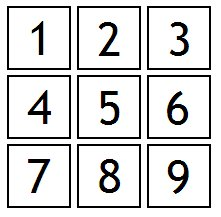
\includegraphics[scale=0.5]{images/tableau_2_dimension.jpg}
\caption{Exemple de tableau en deux dimensions}
\end{figure}

\begin{figure}[htbp]
\centering
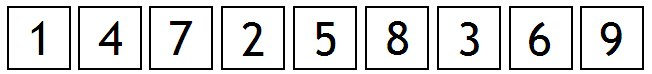
\includegraphics[scale=0.5]{images/column_major_order.jpg}
\caption{Column-major order}
\end{figure}

\begin{figure}[htbp]
\centering
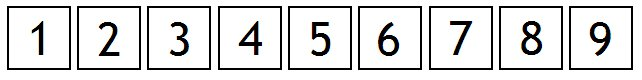
\includegraphics[scale=0.5]{images/row_major_order.jpg}
\caption{Row-major order}
\end{figure}

Le calcul d'adresse à effectuer est une généralisation du calcul vu au
chapitre précédent.

\subsection{Parcours}
\label{parcours}

Le même exemple peut être réalisé à l'aide de deux boucles imbriquées
afin de parcourir le tableau.

\begin{C}
#include <stdio.h>


int main(void)
{
    int tab[2][2] = { { 1, 2 }, { 3, 4 } };
    unsigned i;
    unsigned j;

    for (i = 0; i < 2; ++i)
        for (j = 0; j < 2; ++j)
            printf("tab[%u][%u] = %d\n", i, j, tab[i][j]);

    return 0;
}
\end{C}

\subsection{Tableaux multidimensionnels et fonctions}
\label{tableaux-multidimensionnels-et-fonctions}

\subsubsection{Passage en argument}
\label{passage-en-argument}

Souvenez-vous : sauf exceptions, un tableau est converti en un pointeur
sur son premier élément. Dès lors, qu'obtenons-nous lors du passage d'un
tableau à deux dimensions en argument d'une fonction ? Le premier
élément du tableau est un tableau, donc un pointeur sur\ldots{} Un
tableau (\emph{hé} oui). :p

La syntaxe d'un pointeur sur tableau est la suivante.

\begin{C}
type (*identificateur)[taille];
\end{C}

Vous remarquerez la présence de parenthèses autour du symbole \mybox{*}
et de l'identificateur afin de signaler au compilateur qu'il s'agit d'un
pointeur sur un tableau et non d'un tableau de pointeurs. Également,
notez que la taille du tableau référencé doit être spécifiée. En effet,
sans celle-ci, le compilateur ne pourrait pas opérer correctement le
calcul d'adresses puisqu'il ne connaîtrait pas la taille des éléments
composant le tableau référencé par le pointeur.

La même logique peut-être appliquée pour créer des pointeur sur des
tableaux de tableaux.

\begin{C}
type (*identificateur)[N][M];
\end{C}

Et ainsi de suite jusqu'à ce que mort s'en suive\ldots{} :-°

L'exemple ci-dessous illustre ce qui vient d'être dit en utilisant une
fonction pour afficher le contenu d'un tableau à deux dimensions de
\mybox{int}.

\begin{C}
#include <stdio.h>


void affiche_tableau(int (*tab)[2], unsigned n, unsigned m)
{
    unsigned i;
    unsigned j;

    for (i = 0; i < n; ++i)
        for (j = 0; j < m; ++j)
            printf("tab[%u][%u] = %d\n", i, j, tab[i][j]);
}


int main(void)
{
    int tab[2][2] = { { 1, 2 }, { 3, 4 } };

    affiche_tableau(tab, 2, 2);
    return 0;
}
\end{C}

\subsubsection{Retour de fonction}
\label{retour-de-fonction-2}

Même remarque que pour les tableaux unidimensionnels : attention à la
classe de stockage ! Pour le reste, nous vous laissons admirer la
syntaxe particulièrement dégoûtante d'une fonction retournant un
pointeur sur un tableau de deux \mybox{int}.

\begin{C}
 #include <stdio.h>


int (*tableau(void))[2] /* Ouh ! Que c'est laid ! */
{
    int tab[2][2] = { { 1, 2 }, { 3, 4 } };

    return tab;
}


int main(void)
{
    int (*p)[2] = tableau(); /* Incorrect. */

    printf("%d\n", p[0][0]);
    return 0;
}
\end{C}

\section{Exercices}
\label{exercices-4}

\subsection{Somme des éléments}
\label{somme-des-elements}

Réalisez une fonction qui calcule la somme de tous les éléments d'un
tableau de \mybox{int}.

\begin{C}
 int somme(int *tab, unsigned taille)
{
    unsigned i;
    int res = 0 ;

    for (i = 0; i < taille; ++i)
        res += tableau[i];

    return res;
}
\end{C}

\subsection{Maximum et minimum}
\label{maximum-et-minimum}

Créez deux fonctions : une qui retourne le plus petit élément d'un
tableau de \mybox{int} et une qui renvoie le plus grand élément d'un
tableau de \mybox{int}.

\begin{C}
 int minimum(int *tab, unsigned taille)
{
    unsigned i;
    int min = tab[0];

    for (i = 1; i < taille; ++i)
        if (tab[i] < min)
            min = tab[i];

    return min;
}


int maximum(int *tab, unsigned taille)
{
    unsigned i;
    int max = tab[0];

    for (i = 1; i < taille; ++i)
        if (tab[i] > max)
            max = tab[i];

    return max
}
\end{C}

\subsection{Recherche d'un élément}
\label{recherche-dun-element}

Construisez une fonction qui teste la présence d'une valeur dans un
tableau de \mybox{int}. Celle-ci retournera 1 si un ou plusieurs
éléments du tableau sont égaux à la valeur recherchée, 0 sinon.

\begin{C}
 int find(int * tab, unsigned taille, int val)
{
    unsigned i;

    for (i = 0; i < taille; ++i)
        if (tab[i] == val) 
            return 1;

    return 0;
}
\end{C}

\subsection{Inverser un tableau}
\label{inverser-un-tableau}

Produisez une fonction qui inverse le contenu d'un tableau (le premier
élément devient le dernier, l'avant dernier le deuxième et ainsi de
suite).

\subsubsection{Indice}
\label{indice}

\begin{secretbox}
  Pensez à la fonction \mybox{swap()}
présentée dans le chapitre sur les pointeurs.
\end{secretbox}


\subsubsection{Correction}
\label{correction-16}

\begin{C}
 void swap(int *pa, int *pb)
{
    int tmp;

    tmp = *pa;
    *pa = *pb;
    *pb = tmp;
}


void invert(int *tab , unsigned taille)
{
    unsigned i;

    for (i = 0; i < (taille / 2); ++i)
        swap(tab + i , tab + taille - 1 - i);
    }
}
\end{C}

\subsection{Produit des lignes}
\label{produit-des-lignes}

Composez une fonction qui calcul le produit de la somme des éléments de
chaque ligne d'un tableau de \mybox{int} à deux dimensions (ce tableau
comprend cinq lignes et cinq colonnes).

\begin{C}
 int produit(int (*tab)[5])
{
    unsigned i;
    unsigned j;
    int res = 1;

    for (i = 0; i < 5; ++i)
    {
        int tmp = 0;

        for (j = 0; j < 5; ++j)
            tmp += tab[i][j];

        res *= tmp;
    }

    return res;
}
\end{C}

\subsection{Triangle de Pascal}
\label{triangle-de-pascal}

Les triangles de Pascal sont des objets mathématiques amusants. Voici
une petite animation qui vous expliquera le fonctionnement de ceux-ci.

\begin{figure}[htbp]
\centering
\includegraphics[scale=0.5]{images/PascalTriangleAnimated2-0.png}
%\animategraphics[autoplay,loop]{8}{images/PascalTriangleAnimated2-}{0}{97}
\caption{Explication des triangles de Pascal en image}
\end{figure}

Votre objectif va être de réaliser un programme qui affiche un triangle
de Pascal de la taille souhaitée par l'utilisateur. Pour ce faire, nous
allons diviser le triangle en lignes afin de pouvoir le représenter sous
la forme d'un tableau à deux dimensions. Chaque élément du tableau se
verra attribué soit une valeur du triangle soit zéro pour signaler qu'il
n'est pas utilisé.

La première chose que nous allons faire est donc définir un tableau à
deux dimensions (nous fixerons la taille des dimensions à dix) dont tous
les éléments sont initialisés à zéro. Ensuite, nous allons demandés à
l'utilisateur d'entrer la taille du triangle qu'il souhaite obtenir
(celle-ci ne devra pas être supérieure aux dimensions du tableau).

À présent, passons à la fonction de création du triangle de Pascal.
Celle-ci devra mettre en œuvre l'algorithme suivant.

\begin{C}
N = taille du triangle de Pascal fournie par l’utilisateur

Mettre la première case du tableau à 1

Pour i = 1, i < N, i = i + 1
    Mettre la première case de la ligne à 1

    Pour j = 1, j < i, j = j + 1
         La case [i,j] prend la valeur [i - 1, j - 1] + [i - 1, j]

    Mettre la dernière case de la ligne à 1
\end{C}

Enfin, il vous faudra écrire une petite fonction pour afficher le
tableau ainsi créer.
Bon courage !

\begin{C}
 #include <stdio.h>
#include <stdlib.h>


void triangle_pascal(int (*tab)[10], unsigned taille)
{
    unsigned i;
    unsigned j;

    tab[0][0] = 1;

    for (i = 1; i < taille; ++i)
    {
        tab[i][0] = 1;

        for (j = 1; j < i; ++j)
            tab[i][j] = tab[i - 1][j - 1] + tab[i - 1][j];

        tab[i][i] = 1;
    }
}


void print_triangle(int (*tab)[10], unsigned taille)
{
    unsigned i;
    unsigned j;
    int sp;

    for (i = 0; i < taille; ++i)
    {
        for (sp = taille - 1 - i; sp > 0; --sp)
            printf(" ");

        for (j = 0; j < taille; ++j)
            if (tab[i][j] != 0)
                printf("%d ", tab[i][j]);

        printf("\n");
    }
}


int main(void)
{
    int tab[10][10] = { { 0 } };
    unsigned taille;

    printf("Taille du triangle: ");

    if (scanf("%u", &taille) != 1)
    {
        printf("Mauvaise saisie\n");
        return EXIT_FAILURE;
    }
    else if (taille > 10)
    {
        printf("La taille ne doit pas être supérieure à 10\n");
        return EXIT_FAILURE;
    }

    triangle_pascal(tab, taille);
    print_triangle(tab, taille);  
    return 0;
}
\end{C}

\hrulefill

Dans le chapitre suivant, nous aborderons un nouveau type
d'agrégat, un peu particulier puisqu'il se base sur les tableaux : les
\textbf{chaînes de caractères}.
\chapter{Les chaînes de caractères}
\label{Les chaînes de caractères}

Dans ce chapitre, nous allons apprendre à manipuler du texte ou,
en langage C, des \textbf{chaînes de caractères}

\section{Qu'est-ce qu'une chaîne de caractères ?}
\label{qu-est-ce-qu-une-chaine-de-caractères ?}

Dans le chapitre sur les variables, nous avions mentionné le type \mybox{char}.
Pour rappel, nous vous avions dit que le type \mybox{char} servait surtout
au stockage de caractères, mais que comme ces derniers étaient stockés
dans l'ordinateur sous forme de nombres, il était également possible
d'utiliser ce type pour mémoriser des nombres.

Le seul problème, c'est qu'une variable de type \mybox{char} ne peut
stocker qu'une seule lettre, ce qui est insuffisant pour stocker une
phrase ou même un mot. Si nous voulons mémoriser un texte, nous avons
besoin d'un outil pour rassembler plusieurs lettres dans un seul objet,
manipulable dans notre langage. Cela tombe bien, nous en avons justement
découvert un au chapitre précédent : les tableaux.

C'est ainsi que le texte est géré en C : sous forme de tableaux de
\mybox{char} appelés \textbf{chaînes de caractères} (\emph{strings} en
anglais).

\subsection{Représentation en mémoire}
\label{representation-en-memoire-2}

Néanmoins, il y a une petite subtilité. Une chaîne de caractères est un
plus qu'un tableau : c'est un objet à part entière qui doit être
manipulable directement. Or, ceci n'est possible que si nous connaissons
sa taille.

\subsubsection{Avec une taille intégrée}
\label{avec-une-taille-integree}

Dans certains langages de programmation, les chaines de caractères sont
stockées sous la forme d'un tableau de \mybox{char} auquel est adjoint
un entier pour indiquer sa longueur. Plus précisément, lors de
l'allocation du tableau, le compilateur réserve un élément
supplémentaire pour conserver la taille de la chaîne. Ainsi, il est aisé
de parcourir la chaîne et de savoir quand la fin de celle-ci est
atteinte. De telles chaines de caractères sont souvent appelées des
\emph{Pascal strings}, s'agissant d'une convention apparue avec le
langage de programmation Pascal.

\subsubsection{Avec une sentinelle}
\label{avec-une-sentinelle}

Toutefois, une telle technique limite la taille des chaînes de
caractères à la capacité du type entier utilisé pour mémoriser la
longueur de la chaine. Dans la majorité des cas, il s'agit d'un
\mybox{unsigned\ char}, ce qui donne une limite de 255 caractères
maximum sur la plupart des machines. Pour ne pas subir cette limitation,
les concepteurs du langage C ont adopté une autre solution : la fin de
la chaîne de caractères sera indiquée par un caractère spécial, en
l'occurrence zéro (noté
\mybox{\textquotesingle{}\textbackslash{}0\textquotesingle{}}). Les
chaines de caractères qui fonctionnent sur ce principe sont appelées
\emph{null terminated strings}, ou encore \emph{C strings}.

Cette solution a toutefois deux inconvénients :

\begin{itemize}
\item
  la taille de chaque chaîne doit être calculée en la parcourant
  jusqu'au caractère nul ;
\item
  le programmeur doit s'assurer que chaque chaîne qu'il construit se
  termine bien par un caractère nul.
\end{itemize}

\section{Définition, initialisation et utilisation }
\label{definition,-initialisation-et-utilisation }

\subsection{Définition}
\label{definition-5}

Définir une chaine de caractères, c'est avant tout définir un tableau de
\mybox{char}, ce que nous avons vu au chapitre précédent. L'exemple
ci-dessous définit un tableau de vingt-cinq \mybox{char}.

\begin{C}
char tab[25];
\end{C}

\subsection{Initialisation}
\label{initialisation-6}

Il existe deux méthodes pour initialiser une chaîne de caractères :

\begin{itemize}
\item
  de la même manière qu'un tableau ;
\item
  à l'aide d'une chaîne de caractères littérale.
\end{itemize}

\subsubsection{Avec une liste d'initialisation}
\label{avec-une-liste-dinitialisation}

\subsubsection{Initialisation avec une longueur explicite}
\label{initialisation-avec-une-longueur-explicite-3}

Comme pour n'importe quel tableau, l'initialisation se réalise à l'aide
d'une liste d'initialisation. L'exemple ci-dessous définit donc un
tableau de vingt-cinq \mybox{char} et initialise les sept premiers avec
la suite de lettres « Bonjour ».

\begin{C}
char chaine[25] = { 'B', 'o', 'n', 'j', 'o', 'u', 'r' };
\end{C}

Étant donné que seule une partie des éléments sont initialisés, les
autres sont implicitement mis à zéro, ce qui nous donne une chaîne de
caractères valides puisqu'elle est bien terminée par un caractère nul.
Faites cependant attention à ce qu'il y ait \emph{toujours} de la place
pour un caractère nul.

\subsubsection{Initialisation avec une longueur implicite}
\label{initialisation-avec-une-longueur-implicite-3}

Dans le cas où vous ne spécifiez pas de taille lors de la définition, il
vous faudra ajouter le caractère nul à la fin de la liste
d'initialisation pour obtenir une chaîne valide.

\begin{C}
char chaine[] = { 'B', 'o', 'n', 'j', 'o', 'u', 'r', '\0' };
\end{C}

\subsubsection{Avec une chaîne littérale}
\label{avec-une-chaine-litterale}

Bien que tout à fait valide, cette première solution est toutefois assez
fastidieuse. Aussi, il en existe une seconde : recourir à une
\textbf{chaîne de caractères littérales} pour initialiser un tableau.
Une chaîne de caractères littérales est une suite de caractères entourée
par le symbole \mybox{"}. Nous en avons déjà utilisé auparavant comme
argument des fonctions \mybox{printf()} et \mybox{scanf()}.

Techniquement, une chaîne littérale est un tableau de \mybox{char}
terminé par un caractère nul. Elles peuvent donc s'utiliser comme
n'importe quel autre tableau. Si vous exécutez le code ci-dessous, vous
remarquerez que l'opérateur \mybox{sizeof} retourne bien le nombre de
caractères composant la chaîne littérale (n'oubliez pas de compter le
caractère nul) et que l'opérateur \mybox{{[}{]}} peut effectivement
leur être appliqué.

\begin{C}
#include <stdio.h>


int main(void)
{
    printf("%u\n", (unsigned)sizeof "Bonjour");
    printf("%c\n", "Bonjour"[3]);
    return 0;
}
\end{C}

\begin{C}
8
j
\end{C}

Ces chaînes de caractères littérales peuvent également être utilisées à
la place des listes d'initialisation. En fait, il s'agit de la troisième
et dernière exception à la règle de conversion implicite des tableaux.

\subsubsection{Initialisation avec une longueur explicite}
\label{initialisation-avec-une-longueur-explicite-4}

Dans le cas où vous spécifiez la taille de votre tableau, faites bien
attention à ce que celui-ci dispose de suffisamment de place pour
accueillir la chaîne entière, c'est-à-dire les caractères qui la
composent \emph{et} le caractère nul.

\begin{C}
char chaine[25] = "Bonjour";
\end{C}

\subsubsection{Initialisation avec une longueur implicite}
\label{initialisation-avec-une-longueur-implicite-4}

L'utilisation d'une chaîne littérale pour initialiser un tableau dont la
taille n'est pas spécifiée vous évite de vous soucier du caractère nul
puisque celui-ci fait partie de la chaîne littérale.

\begin{C}
char chaine[] = "Bonjour";
\end{C}

\subsubsection{Utilisation de pointeurs}
\label{utilisation-de-pointeurs}

Nous vous avons dit que les chaînes littérales n'étaient rien d'autre
que des tableaux de \mybox{char} terminés par un caractère nul. Dès
lors, comme pour n'importe quel tableau, il vous est loisible de les
référencer à l'aide de pointeurs.

\begin{C}
char *ptr = "Bonjour";
\end{C}

Néanmoins, les chaînes littérales sont des \emph{constantes}, il vous
est donc impossible de les modifier. L'exemple ci-dessous est donc
incorrect.

\begin{C}
int main(void)
{
    char *ptr = "bonjour";

    ptr[0] = 'B'; /* Incorrect. */
    return 0;
}
\end{C}

\begin{attentionbox}
  Notez bien la différence entre les
exemples précédents qui initialisent un tableau avec le contenu d'une
chaîne littérale (il y a donc copie de la chaîne littérale) et cet
exemple qui initialise un pointeur avec l'adresse du premier élément
d'une chaîne littérale.
\end{attentionbox}


\subsection{Utilisation}
\label{utilisation-1}

Pour le reste, une chaîne de caractères s'utilise comme n'importe quel
autre tableau. Aussi, pour modifier son contenu, il vous faudra accéder
à ses éléments un à un.

\begin{C}
#include <stdio.h>


int main(void)
{
    char chaine[25] = "Bonjour";

    printf("%s\n", chaine);
    chaine[0] = 'A';
    chaine[1] = 'u';
    chaine[2] = ' ';
    chaine[3] = 'r';
    chaine[4] = 'e';
    chaine[5] = 'v';
    chaine[6] = 'o';
    chaine[7] = 'i';
    chaine[8] = 'r';
    chaine[9] = '\0'; /* N'oubliez pas le caractère nul ! */
    printf("%s\n", chaine);
    return 0;
}
\end{C}

\begin{C}
Bonjour
Au revoir
\end{C}


\section{Afficher et récupérer une chaîne de caractères}
\label{afficher-etrecuperer-une-chaine-de-caracteres}

Les chaînes littérales n'étant rien
d'autre que des tableaux de \mybox{char}, il vous est possible
d'utiliser des chaînes de caractères là où vous employiez des chaînes
littérales. Ainsi, les deux exemples ci-dessous afficheront la même
chose.

\begin{C}
#include <stdio.h>


int main(void)
{
    char chaine[] = "Bonjour\n";

    printf(chaine);
    return 0;
}
\end{C}

\begin{C}
#include <stdio.h>


int main(void)
{
    printf("Bonjour\n");
    return 0;
}
\end{C}

\begin{C}
Bonjour
\end{C}

Toutefois, les fonctions \mybox{printf()} et \mybox{scanf()} disposent
d'un indicateur de conversion vous permettant d'afficher ou de demander
une chaîne de caractères : \mybox{s}.

\subsection{Printf}
\label{printf}

L'exemple suivant illustre l'utilisation de cet indicateur de conversion
avec \mybox{printf()} et affiche la même chose que les deux codes
précédents.

\begin{C}
#include <stdio.h>


int main(void)
{
    char chaine[] = "Bonjour";

    printf("%s\n", chaine);
    return 0;
}
\end{C}

\begin{C}
Bonjour
\end{C}

\subsection{Scanf}
\label{scanf-2}

Le même indicateur de conversion peut être utiliser avec
\mybox{scanf()} pour demander à l'utilisateur d'entrer une chaîne de
caractères. Cependant, un problème se pose : étant donné que nous devons
créer un tableau de taille finie pour accueillir la saisie de
l'utilisateur, nous devons impérativement limiter la longueur des
données que nous fournit l'utilisateur.

Pour éviter ce problème, il est possible de spécifier une taille
maximale à la fonction \mybox{scanf()}. Pour ce faire, il vous suffit
de placer un nombre entre le symbole \mybox{\%} et l'indicateur de
conversion \mybox{s}. L'exemple ci-dessous demande à l'utilisateur
d'entrer son prénom (limité à 254 caractères) et affiche ensuite
celui-ci.

\begin{erreurbox}
La fonction \mybox{scanf()} ne décompte
pas le caractère nul final de la limite fournie ! Il vous est donc
nécessaire de lui indiquer la taille de votre tableau diminuée de un.
\end{erreurbox}


\begin{C}
#include <stdio.h>
#include <stdlib.h>


int main(void)
{
    char chaine[255];

    printf("Quel est votre prénom ? ");

    if (scanf("%254s", chaine) != 1)
    {
        printf("Erreur lors de la saisie\n");
        return EXIT_FAILURE;
    }

    printf("Bien le bonjour %s !\n", chaine);
    return 0;
}
\end{C}

\begin{C}
Quel est votre prénom ? Albert
Bien le bonjour Albert !
\end{C}

\subsubsection{Chaîne de caractères avec des espaces}
\label{chaine-de-caracteres-avec-des-espaces}

Sauf qu'en fait, l'indicateur \mybox{s} signifie : « la plus longue
suite de caractère ne comprenant \emph{pas} d'espaces » (les espaces
étant ici entendu comme une suite d'un ou plusieurs des caractères
suivant : \mybox{\textquotesingle{}\ \textquotesingle{}},
\mybox{\textquotesingle{}\textbackslash{}f\textquotesingle{}},
\mybox{\textquotesingle{}\textbackslash{}n\textquotesingle{}},
\mybox{\textquotesingle{}\textbackslash{}r\textquotesingle{}},
\mybox{\textquotesingle{}\textbackslash{}t\textquotesingle{}},
\mybox{\textquotesingle{}\textbackslash{}v\textquotesingle{}})\ldots{}

Autrement dit, si vous entrez « Bonjour tout le monde », la fonction
\mybox{scanf()} va s'arrêter au mot « Bonjour », ce dernier étant suivi
par un espace.

\begin{questionbox}
Comment peut-on récupérer une chaîne complète alors ?
\end{questionbox}


\emph{Eh} bien, il va falloir nous débrouiller avec l'indicateur
\mybox{c} de la fonction \mybox{scanf()} et réaliser nous même une
fonction employant ce dernier au sein d'une boucle. Ainsi, nous pouvons
par exemple créer une fonction recevant un pointeur sur \mybox{char} et
la taille du tableau référencé qui lit un caractère jusqu'à être arrivé
à la fin de la ligne ou à la limite du tableau.

\begin{questionbox}
Et comment sait-on que la lecture est arrivée à la fin d'une ligne ?
\end{questionbox}


La fin de ligne est indiquée par le caractère
\mybox{\textbackslash{}n}.\\
Avec ceci, vous devriez pouvoir construire une fonction adéquate.\\
Allez, \emph{hop}, au boulot et faites gaffe aux retours d'erreur !


\begin{C}
#include <stdio.h>


int lire_ligne(char *chaine, size_t max)
{
    size_t i;
    char c;

    for (i = 0; i < max - 1; ++i)
    {
        if (scanf("%c", &c) != 1)
            return 0;
        else if (c == '\n')
            break;

        chaine[i] = c;
    }

    chaine[i] = '\0';
    return 1;
}


int main(void)
{
    char chaine[255];

    printf("Quel est votre prénom ? ");

    if (lire_ligne(chaine, sizeof chaine))
        printf("Bien le bonjour %s !\n", chaine);

    return 0;
}

\end{C}

\begin{C}
 Quel est votre prénom ? Charles Henri
Bien le bonjour Charles Henri !
\end{C}

\begin{infobox}
  Gardez bien cette fonction sous le
coude, nous allons en avoir besoin pour la suite.
\end{infobox}

\section{Lire et écrire depuis et dans une chaîne de caractères}
\label{lire-et-ecrire-depuis-et-dans-une-chaine-de-caractères}

S'il est possible d'afficher et récupérer une chaîne
de caractères, il est également possible de lire depuis une chaîne et
d'écrire dans une chaîne. À cette fin, deux fonctions qui devraient vous
sembler familières existent : \mybox{sprintf()} et \mybox{sscanf()}.

\subsection{La fonction sprintf}
\label{la-fonction-sprintf}

\begin{C}
int sprintf(char *chaine, char *format, ...);
\end{C}

\begin{infobox}
  Les trois petits points à la fin du
prototype de la fonction signifient que celle-ci attend un nombre
variable d'arguments. Nous verrons ce mécanisme plus en détail dans la
troisième partie du cours.
\end{infobox}


La fonction \mybox{sprintf()} est identique à la fonction
\mybox{printf()} mise à part que celle-ci écrit les données produites
dans une chaîne de caractères au lieu de les afficher à l'écran.
Celle-ci retourne le nombre de caractères écrit (sans compter le
caractère nul final !) ou bien un nombre négatif en cas d'erreur.

Cette fonction peut vous permettre, entre autres, d'écrire un nombre
dans une chaîne de caractères.

\begin{C}
#include <stdio.h>

int main(void)
{
    char chaine[16];
    int n = 64;

    sprintf(chaine, "%d", n);
    printf("%s\n", chaine);
    return 0;
}

\end{C}

\begin{C}
64
\end{C}

\begin{attentionbox}
 La fonction \mybox{sprintf()}
n'effectue \emph{aucune} vérification quant à la taille de la chaîne de
destination, vous devez donc vous assurer qu'elle dispose de
suffisamment de place pour accueillir la chaîne finale (caractère nul
compris !).
\end{attentionbox}


Comment dès lors s'assurer qu'il n'y aura aucun débordement ?
Malheureusement, il n'est pas possible de spécifier une taille comme
avec l'indicateur \mybox{s} de la fonction \mybox{scanf()}, aussi,
deux solutions s'offrent à vous :

\begin{itemize}
\item
  vérifier que le nombre en question ne dépasse pas un certain seuil ;
\item
  compter la quantité de chiffres composant le nombre avant d'appeler
  \mybox{sprintf()}.
\end{itemize}

Ainsi, l'exemple ci-dessous ne pose pas de problèmes puisque nous savons
que si le nombre est inférieur ou égal à 999 999 999, il n'excèdera pas
neuf caractères (\emph{n'oubliez pas de compter le caractère nul final !}).

\begin{C}
#include <stdio.h>
#include <stdlib.h>


int main(void)
{
    char chaine[10];
    long n;

    printf("Entrez un nombre : ");

    if (scanf("%ld", &n) != 1 || n > 999999999L)
    {
        printf("Erreur lors de la saisie\n");
        return EXIT_FAILURE;
    }

    sprintf(chaine, "%ld", n);
    printf("%s\n", chaine);
    return 0;
}
\end{C}

\begin{C}
Entrez un nombre : 890765456789
Erreur lors de la saisie

Entrez un nombre : 5678
5678
\end{C}

\subsection{La fonction sscanf}
\label{la-fonction-sscanf}

\begin{C}
int sscanf(char *chaine, char *format, ...);
\end{C}

La fonction \mybox{sscanf()} est identique à la fonction
\mybox{scanf()} si ce n'est que celle-ci extrait les données depuis une
chaîne de caractères plutôt qu'en provenance d'une saisie de
l'utilisateur. Cette dernière retourne le nombre de conversions réussies
\emph{ou} un nombre inférieur si elles n'ont pas toutes été réalisées
\emph{ou} enfin un nombre négatif en cas d'erreur.

Voici un exemple d'utilisation.

\begin{C}
#include <stdio.h>
#include <stdlib.h>


int main(void)
{
    char chaine[10];
    int n;

    if (sscanf("5 abcd", "%d %9s", &n, chaine) != 2)
    {
        printf("Erreur lors de l'examen de la chaîne\n");
        return EXIT_FAILURE;
    }

    printf("%d %s\n", n, chaine);
    return 0;
}
\end{C}

\begin{C}
5 abcd
\end{C}

\begin{infobox} 
Notez que la fonction \mybox{sscanf()} ne souffre pas du même problème
que \mybox{scanf()} en ce qui concerne de potentiels caractères non lus,
nous y reviendrons un peu plus tard.
\end{infobox}

\section{Les classes de caractères}
\label{les-classes-de-caracteres}

Pour terminer cette partie théorique sur une note un
peu plus légère, sachez que la bibliothèque standard 
fournie unen-tête \mybox{\textless{}ctype.h\textgreater{}}
qui permet de classifier les caractères. Onze fonctions sont
ainsi définies

\begin{C}
int isalnum(int c);
int isalpha(int c);
int iscntrl(int c);
int isdigit(int c);
int isgraph(int c);
int islower(int c);
int isprint(int c);
int ispunct(int c);
int isspace(int c);
int isupper(int c);
int isxdigit(int c);
\end{C}

Chacune d'entre elles attend en argument un caractère et retourne un
nombre positif ou zéro suivant que le caractère fourni appartienne ou
non à la catégorie déterminée par la fonction.

\begin{table}[ht!]
\tiny
\centering
\rowcolors{1}{}{gris-clair-tab}
%\begin{tabularx}{\textwidth}{|l|l|X|X|}\hline
\begin{tabular}{|p{1.5cm}|p{2cm}|p{3.5cm}|p{5.5cm}|}\hline
\rowcolor{gris-tab-entete}\textbf{Fonction} & \textbf{Catégorie} & \textbf{Description} & \textbf{Par défaut}\tabularnewline\hline
%\noindent\parbox[c]{\hsize}isupper &
isupper &
Majuscule & 
Détermine si le caractère entré est une lettre majuscule &
\mybox{\textquotesingle{}A\textquotesingle{}},
\mybox{\textquotesingle{}B\textquotesingle{}},
\mybox{\textquotesingle{}C\textquotesingle{}},
\mybox{\textquotesingle{}D\textquotesingle{}},
\mybox{\textquotesingle{}E\textquotesingle{}},
\mybox{\textquotesingle{}F\textquotesingle{}},
\mybox{\textquotesingle{}G\textquotesingle{}},
\mybox{\textquotesingle{}H\textquotesingle{}},
\mybox{\textquotesingle{}I\textquotesingle{}},
\mybox{\textquotesingle{}J\textquotesingle{}},
\mybox{\textquotesingle{}K\textquotesingle{}},
\mybox{\textquotesingle{}L\textquotesingle{}},
\mybox{\textquotesingle{}M\textquotesingle{}},
\mybox{\textquotesingle{}N\textquotesingle{}},
\mybox{\textquotesingle{}O\textquotesingle{}},
\mybox{\textquotesingle{}P\textquotesingle{}},
\mybox{\textquotesingle{}Q\textquotesingle{}},
\mybox{\textquotesingle{}R\textquotesingle{}},
\mybox{\textquotesingle{}S\textquotesingle{}},
\mybox{\textquotesingle{}T\textquotesingle{}},
\mybox{\textquotesingle{}U\textquotesingle{}},
\mybox{\textquotesingle{}V\textquotesingle{}},
\mybox{\textquotesingle{}W\textquotesingle{}},
\mybox{\textquotesingle{}X\textquotesingle{}},
\mybox{\textquotesingle{}Y\textquotesingle{}} ou
\mybox{\textquotesingle{}Z\textquotesingle{}}\tabularnewline\hline
islower&
Minuscule&
Détermine si le caractère entré est une lettre minuscule&
\mybox{\textquotesingle{}a\textquotesingle{}},
\mybox{\textquotesingle{}b\textquotesingle{}},
\mybox{\textquotesingle{}c\textquotesingle{}},
\mybox{\textquotesingle{}d\textquotesingle{}},
\mybox{\textquotesingle{}e\textquotesingle{}},
\mybox{\textquotesingle{}f\textquotesingle{}},
\mybox{\textquotesingle{}g\textquotesingle{}},
\mybox{\textquotesingle{}h\textquotesingle{}},
\mybox{\textquotesingle{}i\textquotesingle{}},
\mybox{\textquotesingle{}j\textquotesingle{}},
\mybox{\textquotesingle{}k\textquotesingle{}},
\mybox{\textquotesingle{}l\textquotesingle{}},
\mybox{\textquotesingle{}m\textquotesingle{}},
\mybox{\textquotesingle{}o\textquotesingle{}},
\mybox{\textquotesingle{}n\textquotesingle{}},
\mybox{\textquotesingle{}p\textquotesingle{}},
\mybox{\textquotesingle{}q\textquotesingle{}},
\mybox{\textquotesingle{}r\textquotesingle{}},
\mybox{\textquotesingle{}s\textquotesingle{}},
\mybox{\textquotesingle{}t\textquotesingle{}},
\mybox{\textquotesingle{}u\textquotesingle{}},
\mybox{\textquotesingle{}v\textquotesingle{}},
\mybox{\textquotesingle{}w\textquotesingle{}},
\mybox{\textquotesingle{}x\textquotesingle{}},
\mybox{\textquotesingle{}y\textquotesingle{}} ou
\mybox{\textquotesingle{}z\textquotesingle{}}\tabularnewline\hline
isdigit&
Chiffre décimal&
Détermine si le caractère entré est un chiffre décimal&
\mybox{\textquotesingle{}0\textquotesingle{}},
\mybox{\textquotesingle{}1\textquotesingle{}},
\mybox{\textquotesingle{}2\textquotesingle{}},
\mybox{\textquotesingle{}3\textquotesingle{}},
\mybox{\textquotesingle{}4\textquotesingle{}},
\mybox{\textquotesingle{}5\textquotesingle{}},
\mybox{\textquotesingle{}6\textquotesingle{}},
\mybox{\textquotesingle{}7\textquotesingle{}},
\mybox{\textquotesingle{}8\textquotesingle{}} ou
\mybox{\textquotesingle{}9\textquotesingle{}}\tabularnewline\hline
isxdigit&
Chiffre hexadécimal&
Détermine si le caractère entré est un chiffre hexadécimal&
\mybox{\textquotesingle{}0\textquotesingle{}},
\mybox{\textquotesingle{}1\textquotesingle{}},
\mybox{\textquotesingle{}2\textquotesingle{}},
\mybox{\textquotesingle{}3\textquotesingle{}},
\mybox{\textquotesingle{}4\textquotesingle{}},
\mybox{\textquotesingle{}5\textquotesingle{}},
\mybox{\textquotesingle{}6\textquotesingle{}},
\mybox{\textquotesingle{}7\textquotesingle{}},
\mybox{\textquotesingle{}8\textquotesingle{}},
\mybox{\textquotesingle{}9\textquotesingle{}},
\mybox{\textquotesingle{}A\textquotesingle{}},
\mybox{\textquotesingle{}B\textquotesingle{}},
\mybox{\textquotesingle{}C\textquotesingle{}},
\mybox{\textquotesingle{}D\textquotesingle{}},
\mybox{\textquotesingle{}E\textquotesingle{}},
\mybox{\textquotesingle{}F\textquotesingle{}},
\mybox{\textquotesingle{}a\textquotesingle{}},
\mybox{\textquotesingle{}b\textquotesingle{}},
\mybox{\textquotesingle{}c\textquotesingle{}},
\mybox{\textquotesingle{}d\textquotesingle{}},
\mybox{\textquotesingle{}e\textquotesingle{}} ou
\mybox{\textquotesingle{}f\textquotesingle{}}\tabularnewline\hline
isspace&
Espace&
Détermine si le caractère entré est un espace&
\mybox{\textquotesingle{}\ \textquotesingle{}},
\mybox{\textquotesingle{}\textbackslash{}f\textquotesingle{}},
\mybox{\textquotesingle{}\textbackslash{}n\textquotesingle{}},
\mybox{\textquotesingle{}\textbackslash{}r\textquotesingle{}},
\mybox{\textquotesingle{}\textbackslash{}t\textquotesingle{}} ou
\mybox{\textquotesingle{}\textbackslash{}v\textquotesingle{}}\tabularnewline\hline
iscntrl&
Contrôle&
Détermine si le caractère est un caractère dit « de contrôle »&
\mybox{\textquotesingle{}\textbackslash{}0\textquotesingle{}},
\mybox{\textquotesingle{}\textbackslash{}a\textquotesingle{}},
\mybox{\textquotesingle{}\textbackslash{}b\textquotesingle{}},
\mybox{\textquotesingle{}\textbackslash{}f\textquotesingle{}},
\mybox{\textquotesingle{}\textbackslash{}n\textquotesingle{}},
\mybox{\textquotesingle{}\textbackslash{}r\textquotesingle{}},
\mybox{\textquotesingle{}\textbackslash{}t\textquotesingle{}} ou
\mybox{\textquotesingle{}\textbackslash{}v\textquotesingle{}}\tabularnewline\hline
ispunct&
Ponctuation&
Détermine si le caractère entré est un signe de ponctuation&
\mybox{\textquotesingle{}!\textquotesingle{}},
\mybox{\textquotesingle{}"\textquotesingle{}},
\mybox{\textquotesingle{}\#\textquotesingle{}},
\mybox{\textquotesingle{}\%\textquotesingle{}},
\mybox{\textquotesingle{}\&\textquotesingle{}},
\mybox{\textquotesingle{}\textquotesingle{}\textquotesingle{}},
\mybox{\textquotesingle{}(\textquotesingle{}},
\mybox{\textquotesingle{})\textquotesingle{}},
\mybox{\textquotesingle{}*\textquotesingle{}},
\mybox{\textquotesingle{}+\textquotesingle{}},
\mybox{\textquotesingle{},\textquotesingle{}},
\mybox{\textquotesingle{}-\textquotesingle{}},
\mybox{\textquotesingle{}.\textquotesingle{}},
\mybox{\textquotesingle{}/\textquotesingle{}},
\mybox{\textquotesingle{}:\textquotesingle{}},
\mybox{\textquotesingle{};\textquotesingle{}},
\mybox{\textquotesingle{}\textless{}\textquotesingle{}},
\mybox{\textquotesingle{}=\textquotesingle{}},
\mybox{\textquotesingle{}\textgreater{}\textquotesingle{}},
\mybox{\textquotesingle{}?\textquotesingle{}},
\mybox{\textquotesingle{}{[}\textquotesingle{}},
\mybox{\textquotesingle{}\textbackslash{}\textquotesingle{}},
\mybox{\textquotesingle{}{]}\textquotesingle{}},
\mybox{\textquotesingle{}\^{}\textquotesingle{}},
\mybox{\textquotesingle{}\_\textquotesingle{}},
\mybox{\textquotesingle{}\{\textquotesingle{}},
\mybox{\textquotesingle{}\textless{}barre\ droite\textgreater{}\textquotesingle{}},
\mybox{\textquotesingle{}\}\textquotesingle{}} ou
\mybox{\textquotesingle{}\textasciitilde{}\textquotesingle{}}\tabularnewline\hline
isalpha&
Alphabétique&
Détermine si le caractère entré est une lettre alphabétique&
Les deux ensembles de caractères de \mybox{islower()} et
\mybox{isupper()}\tabularnewline\hline
isalnum&
Alphanumérique&
Détermine si le caractère entré est une lettre alphabétique ou un
chiffre décimal&
Les trois ensembles de caractères de \mybox{islower()},
\mybox{isupper()} et \mybox{isdigit()}\tabularnewline\hline
isgraph&
Graphique&
Détermine si le caractère est représentable graphiquement&
Tout sauf l'ensemble de \mybox{iscntrl()} et l'espace
(\mybox{\textquotesingle{}\ \textquotesingle{}})\tabularnewline\hline
isprint&
Affichable&
Détermine si le caractère est « affichable »&
Tout sauf l'ensemble de \mybox{iscntrl()}\tabularnewline\hline
%\end{tabularx}
\end{tabular}
\end{table}

\begin{infobox}
La suite \mybox{\textless{}barre\_droite\textgreater{}} symbolise 
le caractère \mybox{\textbar{}}.
\end{infobox}

Le tableau ci-dessous vous présente chacune de ces onze fonctions ainsi
que les ensembles de caractères qu'elles décrivent. La colonne « par
défaut » vous détail leur comportement en cas d'utilisation de la
\textbf{\emph{locale}} \mybox{C}. Nous reviendrons sur les
\emph{locales} dans la troisième partie de ce cours ; pour l'heure,
considérez que ces fonctions ne retournent un nombre positif que si un
des caractères de leur ensemble « par défaut » leur est fourni en
argument.

L'exemple ci-dessous utilise la fonction \mybox{isdigit()} pour
déterminer si l'utilisateur a bien entré une suite de chiffres.

\begin{C}
#include <stddef.h>
#include <stdio.h>
#include <stdlib.h>

/* lire_ligne() */


int main(void)
{
    char suite[255];
    unsigned i;

    if (!lire_ligne(suite, sizeof suite))
    {
        printf("Erreur lors de la saisie.\n");
        return EXIT_FAILURE;
    }

    for (i = 0; suite[i] != '\0'; ++i)
        if (!isdigit(suite[i]))
        {
            printf("Veuillez entrer une suite de chiffres.\n");
            return EXIT_FAILURE;
        }

    printf("C'est bien une suite de chiffres.\n");
    return 0;
}

\end{C}

\begin{C}
122334
C'est bien une suite de chiffres.

5678a
Veuillez entre une suite de chiffres.
\end{C}

\begin{infobox}
Notez que cet en-tête fourni également deux fonctions : \mybox{tolower()}
et \mybox{toupper()} retournant respectivement la version minuscule ou
majuscule de la lettre entrée. Dans le cas où un caractère autre qu'une
lettre est entré (ou que celle-ci est déjà en minuscule ou en majuscule),
la fonction retourne celui-ci.
\end{infobox}

\section{Exercices }
\label{exercices-5}

\subsection{Palindrome}
\label{palindrome}

Un palindrome est un texte identique lorsqu'il est lu de gauche à droite
et de droite à gauche. Ainsi, le mot \emph{radar} est un palindrome, de
même que les phrases \emph{engage le jeu que je le gagne} et \emph{élu
par cette crapule}. Normalement, il n'est pas tenu compte des accents,
trémas, cédilles ou des espaces. Toutefois, pour cet exercice, nous nous
contenterons de vérifier si un mot donné est un palindrome.

\begin{C}
int palindrome(char *s)
{
    size_t len = 0;
    size_t i;

    while (s[len] != '\0')
        ++len;

    for (i = 0; i < len; ++i)
        if (s[i] != s[len - 1 - i])
            return 0;

    return 1;
}
\end{C}

\subsection{Compter les parenthèses}
\label{compter-les-parentheses}

Écrivez un programme qui lit une ligne et vérifie que chaque parenthèse
ouvrante est bien refermée par la suite.

\begin{C}
Entrez une ligne : printf("%u\n", (unsigned)sizeof(int);
Il manque des parenthèses.
\end{C}

\begin{C}
#include <stdio.h>
#include <stdlib.h>

/* lire_ligne() */


int main(void)
{
    char s[255];
    char *t;
    long n = 0;

    printf("Entrez une ligne : ");

    if (!lire_ligne(s, sizeof s))
    {
        printf("Erreur lors de la saisie.\n");
        return EXIT_FAILURE;
    }

    for (t = s; *t != '\0'; ++t)
        if (*t == '(')
            ++n;
        else if (*t == ')')
            --n;

    if (n == 0)
        printf("Le compte est bon.\n");
    else
        printf("Il manque des parenthèses.\n");

    return 0;
}
\end{C}

\hrulefill

Le chapitre suivant sera l'occasion de mettre en pratique ce que nous
avons vu dans les chapitres précédents à l'aide d'un TP.
\chapter{TP : l'en-tête <string.h>}
\label{tp-:-len-tete-<string.h>}

Les quatre derniers cours ayant été riche en nouveautés, 
posons nous un instant pour mettre en pratique tout cela.

\section{Préparation }
\label{preparation }

Dans le chapitre précédent, nous vous avons dit qu'une chaîne de caractères
se manipulait comme un tableau, à savoir en parcourant ses éléments un à
un. Cependant, si cela s'arrêtait là, cela serait assez gênant. En
effet, la moindre opération sur une chaîne nécessiterait d'accéder à ses
différents éléments, que ce soit une modification, une copie, une
comparaison, etc. Heureusement pour nous, la bibliothèque standard
fourni une suite de fonction nous permettant de réaliser plusieurs
opérations de base sur des chaînes de caractères. Ces fonctions sont
déclarées dans l'en-tête \mybox{\textless{}string.h\textgreater{}}.

L'objectif de ce TP sera de réaliser une version pour chacune des
fonctions de cet en-tête qui vont vous êtes présentées. :)

\subsection{strlen}
\label{strlen-1}

\begin{C}
size_t strlen(char *chaine);
\end{C}

La fonction \mybox{strlen()} vous permet de connaître la taille d'une
chaîne fournie en argument. Celle-ci retourne une valeur de type
\mybox{size\_t}. Notez bien que la longueur retournée ne comprend
\emph{pas} le caractère nul. L'exemple ci-dessous affiche la taille de
la chaîne « Bonjour ».

\begin{C}
#include <stdio.h>
#include <string.h>


int main(void)
{
    printf("Longueur : %u\n", (unsigned)strlen("Bonjour"));
    return 0;
}
\end{C}

\begin{C}
Longueur : 7
\end{C}

\subsection{strcpy}
\label{strcpy-1}

\begin{C}
char *strcpy(char *destination, char *source);
\end{C}

La fonction \mybox{strcpy()} copie le contenu de la chaîne
\mybox{source} dans la chaîne \mybox{destination}, caractère nul
compris. La fonction retourne l'adresse de \mybox{destination}.
L'exemple ci-dessous copie la chaîne « Au revoir » dans la chaîne
\mybox{chaine}.

\begin{C}
#include <stdio.h>


int main(void)
{
    char chaine[25] = "Bonjour\n";

    strcpy(chaine, "Au revoir");
    printf("%s\n", chaine);
    return 0;
}
\end{C}

\begin{C}
Au revoir
\end{C}

\begin{erreurbox}
  La fonction \mybox{strcpy()} n'effectue
\emph{aucune} vérifications. Vous devez donc vous assurer que la chaîne
de destination dispose de suffisamment d'espace pour accueillir la
chaîne qui doit être copiée (caractère nul compris !).
\end{erreurbox}


\subsection{strcat}
\label{strcat-1}

\begin{C}
char *strcat(char *destination, char *source);
\end{C}

La fonction \mybox{strcat()} ajoute le contenu de la chaine
\mybox{source} à celui de la chaîne \mybox{destination}, caractère nul
compris. La fonction retourne l'adresse de \mybox{destination}.
L'exemple ci-dessous ajoute la chaîne « tout le monde » au contenu de la
chaîne \mybox{chaine}.

\begin{C}
#include <stdio.h>
#include <string.h>


int main(void)
{
    char chaine[25] = "Bonjour";

    strcat(chaine, " tout le monde");
    printf("%s\n", chaine);
    return 0;
}
\end{C}

\begin{C}
Bonjour tout le monde
\end{C}

\begin{erreurbox}
  Comme \mybox{strcpy()}, la fonction
\mybox{strcat()} n'effectue \emph{aucune} vérifications. Vous devez
donc vous assurer que la chaîne de destination dispose de suffisamment
d'espace pour accueillir la chaîne qui doit être ajoutée (caractère nul
compris !).
\end{erreurbox}


\subsection{strcmp}
\label{strcmp-1}

\begin{C}
int strcmp(char *chaine1, char *chaine2);
\end{C}

La fonction \mybox{strcmp()} compare deux chaines de caractères. Cette
fonction retourne :

\begin{itemize}
\item
  une valeur positive si la première chaîne est « plus grande » que la
  seconde ;
\item
  zéro si elles sont égales ;
\item
  une valeur négative si la seconde chaîne est « plus grande » que la
  première.
\end{itemize}

\begin{infobox}
  Ne vous inquiétez pas au sujet des
valeurs positives et négatives, nous y reviendront en temps voulu
lorsque nous aborderons les notions de jeux de caractères et d'encodages
dans la troisième partie du cours. En attendant, effectuez simplement
une comparaison entre les deux caractères qui diffèrent.
\end{infobox}


\begin{C}
#include <stdio.h>
#include <string.h>


int main(void)
{
    char chaine1[] = "Bonjour";
    char chaine2[] = "Au revoir";

    if (strcmp(chaine1, chaine2) == 0)
        printf("Les deux chaînes sont identiques\n");
    else
        printf("Les deux chaînes sont différentes\n");

    return 0;
}
\end{C}

\begin{C}
Les deux chaînes sont différentes
\end{C}

\subsection{strchr}
\label{strchr-1}

\begin{C}
char *strchr(char *chaine, int ch);
\end{C}

La fonction \mybox{strchr()} recherche la présence du caractère
\mybox{ch} dans la chaîne \mybox{chaine}. Si celui-ci est rencontré,
la fonction retourne l'adresse de la première occurrence de celui-ci au
sein de la chaîne. Dans le cas contraire, la fonction renvoie un
pointeur nul.

\begin{C}
#include <stddef.h>
#include <stdio.h>
#include <string.h>


int main(void)
{
    char chaine[] = "Bonjour";
    char *p;

    p = strchr(chaine, 'o');

    if (p != NULL)
        printf("La chaîne `%s' contient la lettre %c\n", chaine, *p);

    return 0;
}
\end{C}

\begin{C}
La chaîne `Bonjour' contient la lettre o
\end{C}

\subsection{strpbrk}
\label{strpbrk-1}

\begin{C}
char *strpbrk(char *chaine, char *liste);
\end{C}

La fonction \mybox{strpbrk()} recherche la présence \emph{d'un} des
caractères de la chaîne \mybox{liste} dans la chaîne \mybox{chaine}.
Si un de ceux-ci est rencontré, la fonction retourne l'adresse de la
première occurrence au sein de la chaîne. Dans le cas contraire, la
fonction renvoie un pointeur nul.

\begin{C}
#include <stddef.h>
#include <stdio.h>
#include <string.h>


int main(void)
{
    char chaine[] = "Bonjour";
    char *p;

    p = strpbrk(chaine, "aeiouy");

    if (p != NULL)
        printf("La première voyelle de la chaîne `%s' est : %c\n", chaine, *p);

    return 0;
}
\end{C}

\begin{C}
La première voyelle de la chaîne `Bonjour' est : o
\end{C}

\subsection{strstr}
\label{strstr-1}

\begin{C}
char *strstr(char *chaine1, char *chaine2);
\end{C}

La fonction \mybox{strstr()} recherche la présence de la chaîne
\mybox{chaine2} dans la chaîne \mybox{chaine1}. Si celle-ci est
rencontrée, la fonction retourne l'adresse de la première occurrence de
celle-ci au sein de la chaîne. Dans le cas contraire, la fonction
renvoie un pointeur nul.

\begin{C}
#include <stddef.h>
#include <stdio.h>
#include <string.h>


int main(void)
{
    char chaine[] = "Bonjour";
    char *p;

    p = strstr(chaine, "jour");

    if (p != NULL)
        printf("La chaîne `%s' contient la chaîne `%s'\n", chaine, p);

    return 0;
}
\end{C}

\begin{C}
La chaîne `Bonjour' contient la chaîne `jour'
\end{C}

Ceci étant dit, à vous de jouer. ;)

\begin{infobox}
Par convention, nous commencerons le nom de nos fonctions par la 
lettre « x » afin d'éviter des collisions avec ceux de l'en-tête 
\mybox{\textless{}string.h\textgreater{}}.
\end{infobox}

\subsection{strlen}
\label{strlen}

\begin{C}
size_t xstrlen(char *chaine)
{
    size_t i;

    for (i = 0; chaine[i] != '\0'; ++i)
        ;

    return i;
}
\end{C}

\subsection{strcpy}
\label{strcpy}

\begin{C}
char *xstrcpy(char *destination, char *source)
{
    size_t i;

    for (i = 0; source[i] != '\0'; ++i)
        destination[i] = source[i];

    destination[i] = '\0' /* N'oubliez pas le caractère nul final ! */
    return destination;
}
\end{C}

\subsection{strcat}
\label{strcat}

\begin{C}
char *xstrcat(char *destination, char *source)
{
    size_t i;

    while (*destination != '\0')
        ++destination;

    for (i = 0; source[i] != '\0'; ++i)
        destination[i] = source[i];

    destination[i] = '\0'; /* N'oubliez pas le caractère nul final ! */
    return destination;
}
\end{C}

\subsection{strcmp}
\label{strcmp}

\begin{C}
int xstrcmp(char *chaine1, char *chaine2)
{
    while (*chaine1 == *chaine2)
    {
        if (*chaine1 == '\0')
            return 0;

        ++chaine1;
        ++chaine2;
    }

    return (*chaine1 < *chaine2) ? -1 : 1;
}
\end{C}

\subsection{strchr}
\label{strchr}

\begin{C}
char *xstrchr(char *chaine, int ch)
{
    while (*chaine != '\0')
        if (*chaine == ch)
            return chaine;
        else
            ++chaine;

    return NULL;
}
\end{C}

\subsection{strpbrk}
\label{strpbrk}

\begin{C}
char *xstrpbrk(char *chaine, char *liste)
{
    while (*chaine != '\0')
    {
        char *p = liste;

        while (*p != '\0')
        {
            if (*chaine == *p)
                return chaine;

            ++p;
        }

        ++chaine;
    }

    return NULL;
}
\end{C}

\subsection{strstr}
\label{strstr}

\begin{C}
char *xstrstr(char *chaine1, char *chaine2)
{
    while (*chaine1 != '\0')
    {
        char *s = chaine1;
        char *t = chaine2;

        while (*s != '\0' && *t != '\0')
        {
            if (*s != *t)
                break;
      
            ++s;
            ++t;
        }

        if (*t == '\0')
            return chaine1;

        ++chaine1;
    }

    return NULL;
}
\end{C}

\section{Pour allez plus loin : strtok}
\label{pour-allez-plus-loin-:-strtok}


Pour les plus aventureux d'entre-vous, nous vous
proposons de réaliser en plus la mise en œuvre de la fonction
\mybox{strtok()} qui est un peu plus complexe que ses congénères. :)

\begin{C}
char *strtok(char *chaine, char *liste);
\end{C}

La fonction \mybox{strtok()} est un peu particulière : elle divise la
chaîne \mybox{chaine} en une suite de sous-chaînes délimitée par
\emph{un} des caractères présent dans la chaîne \mybox{liste}. En fait,
cette dernière remplace les caractères de la chaîne \mybox{liste} par
des caractères nuls dans la chaîne \mybox{chaine} (elle modifie donc la
chaîne \mybox{chaine} !) et renvoie les différentes sous-chaînes ainsi
créées au fur et à mesure de ses appels.

Lors des appels subséquents, la chaîne \mybox{chaine} doit être un
pointeur nul afin de signaler à \mybox{strtok()} que nous souhaitons la
sous-chaîne suivante. S'il n'y a plus de sous-chaîne ou qu'aucun
caractère de la chaîne \mybox{liste} n'est trouvé, celle-ci retourne un
pointeur nul.

L'exemple ci-dessous tente de scinder la chaîne « un, deux, trois » en
trois sous-chaînes.

\begin{C}
#include <stddef.h>
#include <stdio.h>
#include <string.h>


int main(void)
{
    char chaine[] = "un, deux, trois";
    char *p;
    unsigned i;

    p = strtok(chaine, ", ");

    for (i = 0; p != NULL; ++i)
    {
        printf("%u : %s\n", i, p);
        p = strtok(NULL, ", ");
    }

    return 0;
}
\end{C}

\begin{C}
0 : un
1 : deux
2 : trois
\end{C}

La fonction \mybox{strtok()} étant un peu plus complexe que les autres,
voici une petite marche à suivre pour réaliser cette fonction.

\begin{itemize}
\item
  regarder si la chaîne fournie (ou la sous-chaîne suivante) contient,
  \emph{à son début}, des caractères présent dans la seconde chaîne. Si
  oui, ceux-ci doivent être passés ;
\item
  si la fin de la (sous-)chaîne est atteinte, retourner un pointeur nul
  ;
\item
  parcourir la chaîne fournie (ou la sous-chaîne courante) jusqu'à
  rencontrer un des caractères composant la seconde chaîne. Si un
  caractère est rencontré, le remplacer par un caractère nul, conserver
  la position actuelle dans la chaîne et retourner la sous-chaîne ainsi
  créée (\emph{sans} les éventuels caractères passés au début) ;
\item
  si la fin de la (sous-)chaîne est atteinte, retourner la (sous-)chaîne
  (\emph{sans} les éventuels caractères passés au début).
\end{itemize}

\begin{infobox}
  Vous aurez besoin d'une variable de
classe de stockage statique pour réaliser cette fonction. Également,
l'instruction \mybox{goto} pourra vous être utile.
\end{infobox}


\subsection{Correction}
\label{correction-17}

\begin{C}
char *xstrtok(char *chaine, char *liste)
{
    static char *dernier;
    char *base = (chaine != NULL) ? chaine : dernier;
    char *s;
    char *t;

    if (base == NULL)
        return NULL;

separateur_au_debut:
    for (t = liste; *t != '\0'; ++t)
        if (*base == *t)
        {
            ++base;
            goto separateur_au_debut;
        }

    if (*base == '\0')
    {
        dernier = NULL;
        return NULL;
    }

    for (s = base; *s != '\0'; ++s)
        for (t = liste; *t != '\0'; ++t)
            if (*s == *t)
            {
                *s = '\0';
                dernier = s + 1;
                return base;
            }

    dernier = NULL;
    return base;
}
\end{C}

\hrulefill

le chapitre suivant, nous aborderons le mécanisme de
l'\textbf{allocation dynamique de mémoire}.
\chapter{L'allocation dynamique}
\label{lallocation-dynamique}

Il est à présent temps d'aborder la troisième et dernière utilisation
majeure des pointeurs : l'allocation dynamique de mémoire.

Comme nous vous l'avons dit dans le chapitre sur les pointeurs, il n'est
pas toujours possible de savoir quelle quantité de mémoire sera utilisée
par un programme. Par exemple, si vous demandez à l'utilisateur de vous
fournir un tableau, vous devrez lui fixer une limite, ce qui pose deux
problèmes :

\begin{itemize}
\item
  la limite en elle-même, qui ne convient peut-être pas à votre
  utilisateur ;
\item
  l'utilisation excessive de mémoire du fait que vous réservez un
  tableau d'une taille fixée à l'avance.
\end{itemize}

De plus, si vous utilisez un tableau de classe de stockage statique,
alors cette quantitée de mémoire superflue sera inutilisable jusqu'à la
fin de votre programme.

Or, un ordinateur ne dispose que d'une quantité limitée de mémoire vive,
il est donc important de ne pas en réserver abusivement. L'allocation
dynamique permet de réserver une partie de la mémoire vive inutilisée
pour stocker des données et de libérer cette même partie une fois
qu'elle n'est plus nécessaire.

\section{La notion d'objet}
\label{la-notion-dobjet}

Jusqu'à présent, nous avons toujours recouru au système de types et de
variables du langage C pour stocker nos données sans jamais vraiment
nous soucier de ce qui se passait « en-dessous ».

Il est à présent temps de lever une partie de ce voile en abordant la
notion d'\textbf{objet}.

En C, un objet est une zone mémoire pouvant contenir des données et est
composé d'une suite contiguë d'un ou plusieurs multiplets. En fait, tous
les types du langage C manipulent des objets. La différence entre les
types tient simplement en la manière dont ils répartissent les données
au sein de ces objets, ce qui est appelé leur \textbf{représentation}
(celle-ci sera abordée dans la troisième partie du cours). Ainsi, la
valeur 1 n'est pas représentée de la même manière dans un objet de type
\mybox{int} que dans un objet de type \mybox{double}.

Un objet étant une suite contiguë de multiplets, il est possible d'en
examiner le contenu en lisant ses multiplets un à un. Ceci peut se
réaliser en C à l'aide de l'adresse de l'objet et d'un pointeur sur
\mybox{unsigned\ char}, le type \mybox{char} du C ayant
\emph{toujours} la taille d'un multiplet. Notez qu'il est
\emph{impératif} d'utiliser la version non signée du type \mybox{char}
afin d'éviter des problèmes de conversions.

L'exemple ci-dessous affiche les multiplets composant un objet de type
\mybox{int} et un objet de type \mybox{double} en hexadécimal.

\begin{C}
#include <stdio.h>


int main(void)
{
    int n = 1;
    double f = 1.;
    unsigned char *byte;
    unsigned i;

    byte = (unsigned char *)&n;

    for (i = 0; i < sizeof n; ++i)
        printf("%x ", byte[i]);

    printf("\n");
    byte = (unsigned char *)&f;

    for (i = 0; i < sizeof f; ++i)
        printf("%x ", byte[i]);

    printf("\n");
    return 0;
}
\end{C}

\begin{C}
1 0 0 0 
0 0 0 0 0 0 f0 3f 
\end{C}

\begin{infobox}
Il se peut que vous n'obteniez pas le
même résultat que nous, ce dernier dépends de votre machine.
\end{infobox}

Comme vous le voyez, la représentation de la valeur 1 n'est pas du tout
la même entre le type \mybox{int} et le type \mybox{double}.

\section{Malloc et consoeurs}
\label{malloc-et-consoeurs}

La bibliothèque standard fourni trois fonctions vous permettant d'allouer 
de la mémoire : \mybox{malloc()}, \mybox{calloc()} et \mybox{realloc()} et 
une vous permettant de la libérer : \mybox{free()}. Ces quatres fonctions 
sont déclarées dans l'en-tête \mybox{\textless{}stdlib.h\textgreater{}}.

\subsection{malloc}
\label{malloc}

\begin{C}
void *malloc(size_t taille);
\end{C}

La fonction \mybox{malloc()} vous permet d'allouer un objet de la
taille fournie en argument (qui représente un nombre de multiplets) et
retourne l'adresse de cet objet sous la forme d'un pointeur générique.
En cas d'échec de l'allocation, elle retourne un pointeur nul.

\begin{attentionbox} 
 Vous devez \emph{toujours} vérifier le
retour d'une fonction d'allocation afin de vous assurer que vous
manipulez bien un pointeur valide.
\end{attentionbox}


\subsubsection{Allocation d'un objet}
\label{allocation-dun-objet}

Dans l'exemple ci-dessous, nous réservons un objet de la taille d'un
\mybox{int}, nous y stockons ensuite la valeur dix et l'affichons. Pour
cela, nous utilisons un pointeur sur \mybox{int} qui va se voir
affecter l'adresse de l'objet ainsi alloué et qui va nous permettre de
le manipuler comme nous le ferions s'il référençait une variable de type
\mybox{int}.

\begin{C}
#include <stdio.h>
#include <stdlib.h>


int main(void)
{
    int *p;

    p = malloc(sizeof(int));

    if (p == NULL)
    {
        printf("Échec de l'allocation\n");
        return EXIT_FAILURE;
    }

    *p = 10;
    printf("%d\n", *p);
    return 0;
}
\end{C}

\begin{C}
10
\end{C}

\subsubsection{Allocation d'un tableau}
\label{allocation-dun-tableau}

Pour allouer un tableau, vous devez réserver un bloc mémoire de la
taille d'un élément multiplié par le nombre d'éléments composant le
tableau. L'exemple suivant alloue un tableau de dix \mybox{int},
l'initialise et affiche son contenu.

\begin{C}
#include <stdio.h>
#include <stdlib.h>


int main(void)
{
    int *p;
    unsigned i;

    p = malloc(sizeof(int) * 10);

    if (p == NULL)
    {
        printf("Échec de l'allocation\n");
        return EXIT_FAILURE;
    }

    for (i = 0; i < 10; ++i)
    {
        p[i] = i * 10;
        printf("p[%u] = %d\n", i, p[i]);
    }

    return 0;
}
\end{C}

\begin{C}
p[0] = 0
p[1] = 10
p[2] = 20
p[3] = 30
p[4] = 40
p[5] = 50
p[6] = 60
p[7] = 70
p[8] = 80
p[9] = 90
\end{C}

\begin{infobox} 
 Autrement dit et de manière plus
générale : pour allouer dynamiquement un objet de type \textbf{T}, il
vous faut créer un pointeur sur le type \textbf{T} qui conservera son
adresse.
\end{infobox}


\begin{erreurbox} 
 La fonction \mybox{malloc()} n'effectue
\emph{aucune} initialisation, le contenu du bloc alloué est donc
indéterminé.
\end{erreurbox}


\subsection{free}
\label{free}

\begin{C}
void free(void *ptr);
\end{C}

La fonction \mybox{free()} libère le bloc précédemment alloué par une
fonction d'allocation dont l'adresse est fournie en argument. Dans le
cas où un pointeur nul lui est fourni, elle n'effectue aucune opération.

\begin{attentionbox}
Retenez bien la règle suivante : à chaque appel à une fonction d'allocation 
doit correspondre un appel à la fonction \mybox{free()}.
\end{attentionbox}


Dès lors, nous pouvons compléter les exemples précédents comme suit.

\begin{C}
#include <stdio.h>
#include <stdlib.h>


int main(void)
{
    int *p;

    p = malloc(sizeof(int));

    if (p == NULL)
    {
        printf("Échec de l'allocation\n");
        return EXIT_FAILURE;
    }

    *p = 10;
    printf("%d\n", *p);
    free(p);
    return 0;
}
\end{C}

\begin{C}
#include <stdio.h>
#include <stdlib.h>


int main(void)
{
    int *p;
    unsigned i;

    p = malloc(sizeof(int) * 10);

    if (p == NULL)
    {
        printf("Échec de l'allocation\n");
        return EXIT_FAILURE;
    }

    for (i = 0; i < 10; ++i)
    {
        p[i] = i * 10;
        printf("p[%u] = %d\n", i, p[i]);
    }

    free(p);
    return 0;
}
\end{C}

\begin{infobox}
Remarquez que même si le deuxième exemple alloue un tableau, il 
n'y a bien eu qu'\emph{une seule} allocation. Un seul appel à la 
fonction \mybox{free()} est donc nécessaire.
\end{infobox}


\subsection{calloc}
\label{calloc}

\begin{C}
void *calloc(size_t nombre, size_t taille);
\end{C}

La fonction \mybox{calloc()} attends deux arguments : le nombre
d'éléments à allouer et la taille de chacun de ces éléments.
Techniquement, elle revient au même que d'appelé \mybox{malloc()} comme
suit.

\begin{C}
malloc(nombre * taille);
\end{C}

à un détail près : \emph{le bloc de mémoire ainsi alloué est initialisé
à zéro}.

\begin{erreurbox}
Faites attention : cette initialisation n'est pas similaire à celle des 
variables de classe de stockage statique ! À l'inverse de ces dernières 
qui seront soit initialisées à zéro, soit seront des pointeurs nuls, 
l'initialisation réalisée par la fonction \mybox{calloc()} ne s'applique 
qu'aux entiers ou aux chaînes de caractères (nous verrons cela plus en détails 
dans la troisième partie du cours).
\end{erreurbox}

\subsection{realloc}
\label{realloc}

\begin{C}
void *realloc(void *p, size_t taille);
\end{C}

La fonction \mybox{realloc()} libère un bloc de mémoire précédemment
alloué, en réserve un nouveau de la taille demandée et copie le contenu
de l'ancien objet dans le nouveau. Dans le cas où la taille demandée est
inférieure à celle du bloc d'origine, le contenu de celui-ci sera copié
à hauteur de la nouvelle taille. À l'inverse, si la nouvelle taille est
supérieure à l'ancienne, l'excédant n'est pas initialisé.

La fonction attends deux arguments : l'adresse d'un bloc précédemment
alloué à l'aide d'une fonction d'allocation et la taille du nouveau bloc
à allouer. Elle retourne l'adresse du nouveau bloc ou un pointeur nul en
cas d'erreur.

L'exemple ci-dessous alloue un tableau de dix \mybox{int} et utilise
\mybox{realloc()} pour agrandir celui-ci à vingt \mybox{int}.

\begin{C}
#include <stdio.h>
#include <stdlib.h>


int main(void)
{
    int *p;
    int *tmp;
    unsigned i;

    p = malloc(sizeof(int) * 10);

    if (p == NULL)
    {
        printf("Échec de l'allocation\n");
        return EXIT_FAILURE;
    }

    for (i = 0; i < 10; ++i)
        p[i] = i * 10;

    tmp = realloc(p, sizeof(int) * 20);

    if (tmp == NULL)
    {
        printf("Échec de l'allocation\n");
        return EXIT_FAILURE;
    }

    p = tmp;

    for (i = 10; i < 20; ++i)
        p[i] = i * 10;

    for (i = 0; i < 20; ++i)
        printf("p[%u] = %d\n", i, p[i]);

    free(p);
    return 0;
}
\end{C}

\begin{C}
p[0] = 0
p[1] = 10
p[2] = 20
p[3] = 30
p[4] = 40
p[5] = 50
p[6] = 60
p[7] = 70
p[8] = 80
p[9] = 90
p[10] = 100
p[11] = 110
p[12] = 120
p[13] = 130
p[14] = 140
p[15] = 150
p[16] = 160
p[17] = 170
p[18] = 180
p[19] = 190
\end{C}

Remarquez que nous avons utilisé une autre variable, \mybox{tmp}, pour
vérifier le retour de la fonction \mybox{realloc()}. En effet, si nous
avions procéder comme ceci.

\begin{C}
p = realloc(p, sizeof(int) * 20);
\end{C}

il nous aurait été impossible de libérer le bloc mémoire référencé par
\mybox{p} en cas d'erreur puisque celui-ci serait devenu un pointeur
nul. Il est donc \emph{impératif} d'utiliser une seconde variable afin
d'éviter des \MYhref{http://fr.wikipedia.org/wiki/Fuite_de_mémoire}{fuites
de mémoire}.

\section{Les tableaux multidimensionnels}
\label{les-tableaux-multidimensionnels-2}

L'allocation de tableaux multidimensionnels est un petit peu
plus complexe que celles des autres objets. Techniquement, il existe
deux solutions : l'allocation d'un seul bloc de mémoire (comme pour les
tableaux simples) et l'allocation de plusieurs tableaux eux-mêmes
référencés par les éléments d'un autre tableau.

\subsection{Allocation en un bloc}
\label{allocation-en-un-bloc}

Comme pour un tableau simple, il vous est possible d'allouer un bloc de
mémoire dont la taille correspond à la multiplication des longueurs de
chaque dimension, elle-même multipliée par la taille d'un élément.
Toutefois, cette solution vous contraint à effectuer une partie du
calcul d'adresse vous-même puisque vous allouez en fait un seul tableau.

L'exemple ci-dessous illustre ce qui vient d'être dit en allouant un
tableau à deux dimensions de trois fois trois \mybox{int}.

\begin{C}
#include <stdio.h>
#include <stdlib.h>


int main(void)
{
    int *p;
    unsigned i;
    unsigned j;

    p = malloc(3 * 3 * sizeof(int));

    if (p == NULL)
    {
        printf("Échec de l'allocation\n");
        return EXIT_FAILURE;
    }

    for (i = 0; i < 3; ++i)
        for (j = 0; j < 3; ++j)
        {
            p[(i * 3) + j] = (i * 3) + j;
            printf("p[%u][%u] = %d\n", i, j, p[(i * 3) + j]);
        }

    free(p);
    return 0;
}
\end{C}

\begin{C}
p[0][0] = 0
p[0][1] = 1
p[0][2] = 2
p[1][0] = 3
p[1][1] = 4
p[1][2] = 5
p[2][0] = 6
p[2][1] = 7
p[2][2] = 8
\end{C}

Comme vous le voyez, une partie du calcul d'adresse doit être effectué
en multipliant le premièr indice par la longueur de la première
dimension, ce qui permet d'arriver à la bonne « ligne ». Ensuite, il ne
reste plus qu'à sélectionner le bon élément de la ligne à l'aide du
second indice.

Bien qu'un petit peu plus complexe quant à l'accès aux éléments, cette
solution à l'avantage de n'effectuer qu'une seule allocation de mémoire.

\subsection{Allocation de plusieurs tableaux}
\label{allocation-de-plusieurs-tableaux}

La seconde solution consiste à allouer plusieurs tableaux plus un autre
qui les référencera. Dans le cas d'un tableau à deux dimensions, cela
signifie allouer un tableau de pointeurs dont chaque élément se verra
affecter l'adresse d'un tableau également alloué dynamiquement. Cette
technique nous permet d'accéder aux éléments des différents tableaux de
la même manière que pour un tableau multidimensionnel puisque nous
utilisons cette fois plusieurs tableaux.

L'exemple ci-dessous revient au même que le précédent, mais utilise le
procédé qui vient d'être décrit. Notez que puisque nous réservons un
tableau de pointeurs sur \mybox{int}, l'adresse de celui-ci doit être
stockée dans un pointeur de pointeur sur \mybox{int} (rappelez-vous la
règle générale lors de la présentation de la fonction
\mybox{malloc()}).

\begin{C}
#include <stdio.h>
#include <stdlib.h>


int main(void)
{
    int **p;
    unsigned i;
    unsigned j;

    p = malloc(3 * sizeof(int *));

    if (p == NULL)
    {
        printf("Échec de l'allocation\n");
        return EXIT_FAILURE;
    }

    for (i = 0; i < 3; ++i)
    {
        p[i] = malloc(3 * sizeof(int));

        if (p[i] == NULL)
        {
            printf("Échec de l'allocation\n");
            return EXIT_FAILURE;
        }
    }

    for (i = 0; i < 3; ++i)
        for (j = 0; j < 3; ++j)
        {
            p[i][j] = (i * 3) + j;
            printf("p[%u][%u] = %d\n", i, j, p[i][j]);
        }

    for (i = 0; i < 3; ++i)
        free(p[i]);

    free(p);
    return 0;
}
\end{C}

Si cette solution permet de faciliter l'accès aux différents éléments,
elle présente toutefois l'inconvénient de réaliser plusieurs allocations
et donc de nécessiter plusieurs appels à la fonction \mybox{free()}.

\hrulefill

Ce chapitre nous aura permis de découvrir la notion d'objet ainsi que le
mécanisme de l'allocation dynamique. Dans le chapitre suivant, nous
verrons comment manipuler les \textbf{fichiers}.
\chapter{Les fichiers (1)}
\label{les-fichiers-(1)}

Jusqu'à présent, nous n'avons manipulé que des données en
mémoire, ce qui nous empêchait de les stocker de manière permanente.
Dans ces deux chapitres, nous allons voir comment conserver des
informations de manière permanente à l'aide des fichiers.

\section{Les fichiers}
\label{les-fichiers}

En informatique, un fichier est un ensemble d'informations stockées 
sur un support, réuni sous un même nom et manipulé comme une unité.

\subsection{Extension de fichier}
\label{extension-de-fichier}

Le contenu de chaque fichier est lui-même organisé suivant un format qui
dépend des données qu'il contient. Il en existe une pléthore pour chaque
type de données :

\begin{itemize}
\item
  audio : Ogg, MP3, MP4, FLAC, Wave, etc. ;
\item
  vidéo : Ogg, WebM, MP4, AVI, etc. ;
\item
  documents : ODT, DOC et DOCX, XLS et XLSX, PDF, Postscript, etc.
\end{itemize}

Afin d'aider l'utilisateur, ces formats sont le plus souvent indiqués à
l'aide d'une \textbf{extension} qui se traduit par un suffixe ajouter au
nom de fichier. Toutefois, cette extension est purement
\emph{indicative} et \emph{facultative}, elle n'influence \emph{en rien}
le contenu du fichier. Son seul objectif est d'aider à déterminer le
type de contenu d'un fichier.

\subsection{Système de fichiers}
\label{systeme-de-fichiers}

Afin de faciliter leur localisation et leur gestion, les fichiers sont
classés et organisés sur leur support suivant un \textbf{système de
fichiers}. C'est lui qui permet à l'utilisateur de répartir ses fichiers
dans une arborescence de dossiers et de localiser ces derniers à partir
d'un chemin d'accès.

\subsubsection{Le chemin d'accès}
\label{le-chemin-dacces}

Le chemin d'accès d'un fichier est une suite de caractères décrivant la
position de celui-ci dans le système de fichiers. Un chemin d'accès se
compose au minimum du nom du fichier visé et au maximum de la suite de
tous les dossiers qu'il est nécessaire de traverser pour l'atteindre
depuis le \textbf{répertoire racine}. Ces éventuels dossiers à traverser
sont séparés par un caractère spécifique qui est \mybox{/} sous
Unixoïde et \mybox{\textbackslash{}} sous Windows.

La \textbf{racine} d'un système de fichier est le point de départ de
l'arborescence des fichiers et dossiers. Sous Unixoïdes, il s'agit du
répertoire \mybox{/} tandis que sous Windows, chaque lecteur est une
racine (comme \mybox{C:} par exemple). Si un chemin d'accès commence
par la racine, alors celui-ci est dit \textbf{absolu} car il permet
d'atteindre le fichier depuis n'importe quelle position dans
l'arborescence. Si le chemin d'accès ne commence pas par la racine, il
est dit \textbf{relatif} et ne permet de parvenir au fichier que depuis
un point précis dans la hiérarchie de fichiers.

Ainsi, si nous souhaitons accéder à un fichier nommé « texte.txt » situé
dans le dossier « documents » lui-même situé dans le dossier «
utilisateur » qui est à la racine, alors le chemin d'accès absolu vers
ce fichier serait \mybox{/utilisateur/documents/texte.txt} sous
Unixoïde et
\mybox{C:\textbackslash{}utilisateur\textbackslash{}documents\textbackslash{}texte.txt}
sous Windows (à supposer qu'il soit sur le lecteur \mybox{C:}).
Toutefois, si nous sommes déjà dans le dossier « utilisateur », alors
nous pouvons y accéder à l'aide du chemin relatif
\mybox{documents/texte.txt} ou
\mybox{documents\textbackslash{}texte.txt}. Néanmoins, ce chemin
relatif n'est utilisable que si nous sommes dans le dossier «
utilisateur ».

\subsubsection{Métadonnées}
\label{metadonnees}

Également, le système de fichier se charge le plus souvent de conserver
un certain nombre de données concernant chaque fichier comme :

\begin{itemize}
\item
  sa taille ;
\item
  ses droits d'accès (les utilisateurs autorisés à le manipuler) ;
\item
  la date de dernier accès ;
\item
  la date de dernière modification ;
\item
  etc.
\end{itemize}

\section{Les flux : un peu de théorie}
\label{les-flux-:-un-peu-de-theorie}

La bibliothèque standard vous fourni différentes fonctions pour manipuler
les fichiers, toutes déclarées dans l'en-tête
\mybox{\textless{}stdio.h\textgreater{}}. Toutefois, celles-ci
manipulent non pas des fichiers, mais des \textbf{flux} de données en
provenance ou à destination de fichiers. Ces flux peuvent être de deux
types :

\begin{itemize}
\item
  des flux de textes qui sont des suites de caractères terminées par un
  caractère de fin de ligne (\mybox{\textbackslash{}n}) et formant
  ainsi des lignes ;
\item
  des flux binaires qui sont des suites de multiplets.
\end{itemize}

\subsection{Pourquoi utiliser des flux ?}
\label{pourquoi-utiliser-des-flux-?}

Pourquoi recourir à des flux plutôt que de manipuler directement des
fichiers nous demanderez-vous ? Pour deux raisons : les disparités entre
système d'exploitation quant à la représentation des lignes et la
lourdeur des opérations de lecture et d'écriture.

\subsubsection{Disparités entre systèmes d'exploitation}
\label{disparites-entre-systemes-dexploitation}

Les différents systèmes d'exploitation ne représentent pas les lignes de
la même manière :

\begin{itemize}
\item
  sous Mac OS (avant Mac OS X), la fin d'une ligne était indiquée par le
  caractère \mybox{\textbackslash{}r} ;
\item
  sous Windows, la fin de ligne est indiquée par la suite de caractères
  \mybox{\textbackslash{}r\textbackslash{}n} ;
\item
  sous Unixoïdes (GNU/Linux, *BSD, Mac OS X, Solaris, etc.), la fin de
  ligne est indiquée par le caractère \mybox{\textbackslash{}n}.
\end{itemize}

Aussi, si nous manipulions directement des fichiers, nous devrions
prendre en compte ces disparités, ce qui rendrait notre code nettement
plus pénible à rédiger. En passant par les fonctions de la bibliothèque
standard, nous évitons ce casse-tête car celle-ci remplace le ou les
caractères de fin de ligne par un \mybox{\textbackslash{}n} (ce que
nous avons pu expérimenter avec les fonctions \mybox{printf()} et
\mybox{scanf()}) et inversément.

\subsubsection{Lourdeur des opérations de lecture et d'écriture}
\label{lourdeur-des-operations-de-lecture-et-decriture}

Lire depuis un fichier ou écrire dans un fichier signifie le plus
souvent accéder au disque dur. Or, rappelez-vous, il s'agit de la
mémoire la plus lente d'un ordinateur. Dès lors, si pour lire une ligne
il était nécessaire de récupérer les caractères un à un depuis le disque
dur, cela prendrait un temps fou.

Pour éviter ce problème, les flux de la bibliothèque standard recourent
à un mécanisme appelé la \textbf{temporisation} ou \textbf{mémorisation}
(\emph{buffering} en anglais). La bibliothèque standard fournit deux
types de temporisation :

\begin{itemize}
\item
  la temporisation par blocs ;
\item
  et la temporisation par lignes.
\end{itemize}

Avec la \textbf{temporisation par blocs}, les données sont récupérées
depuis le fichier et écrites dans le fichier sous forme de blocs d'une
taille déterminée. L'idée est la suivante : plutôt que de lire les
caractères un à un, nous allons demander un bloc de données d'une taille
déterminée que nous conserverons en mémoire vive pour les accès
suivants. Cette technique est également utilisée lors des opérations
d'écritures : les données sont stockées en mémoire jusqu'à ce qu'elles
atteignent la taille d'un bloc. Ainsi, le nombre d'accès au disque dur
sera limité à la taille totale du fichier à lire (ou des données à
écrire) divisée par la taille d'un bloc.

La \textbf{temporisation par lignes}, comme son nom l'indique, se
contente de mémoriser une ligne. Techniquement, celle-ci est utilisée
lorsque le flux est associé à un périphérique interactif comme un
terminal. En effet, si nous appliquions la temporisation par blocs pour
les entrées de l'utilisateur, ce dernier devrait entrer du texte jusqu'à
atteindre la taille d'un bloc. Pareillement, nous devrions attendre
d'avoir écrit une quantité de données égale à la taille d'un bloc pour
que du texte soit affiché à l'écran. Cela serait assez gênant et peu
interactif\ldots{} À la place, c'est la temporisation par lignes qui est
utilisée : les données sont stockées jusqu'à ce qu'un caractère de fin
de ligne soit rencontré (\mybox{\textbackslash{}n}, donc) ou jusqu'à ce
qu'une taille maximale soit atteinte.

La bibliothèque standard vous permet également de ne pas temporiser les
données en provenance ou à destination d'un flux.

\subsection{stdin, stdout et stderr}
\label{stdin-stdout-et-stderr}

Par défaut, trois flux \emph{de texte} sont ouverts lors du démarrage
d'un programme et sont déclarés dans l'en-tête
\mybox{\textless{}stdio.h\textgreater{}} : \mybox{stdin},
\mybox{stdout} et \mybox{stderr}.

\begin{itemize}
\item
  \mybox{stdin} correspond à l'\textbf{entrée standard}, c'est-à-dire
  le flux depuis lequel vous pouvez récupérer les informations fournies
  par l'utilisateur.
\item
  \mybox{stdout} correspond à la \textbf{sortie standard}, il s'agit du
  flux vous permettant de transmettre des informations à l'utilisateur
  qui seront le plus souvent affichées dans le terminal.
\item
  \mybox{stderr} correspond à la \textbf{sortie d'erreur standard},
  c'est ce flux que vous devez privilégier lorsque vous souhaitez
  transmettre des messages d'erreurs ou des avertissements à l'attention
  de l'utilisateur (nous verrons comment l'utiliser un peu plus tard
  dans ce chapitre). Comme pour \mybox{stdout}, ces données sont le
  plus souvent affichées dans le terminal.
\end{itemize}

Les flux \mybox{stdin} et \mybox{stdout} sont temporisés par lignes
(sauf s'ils sont associés à des fichiers au lieu de périphériques
interactifs, auxquels cas ils seront temporisés par blocs) tandis que le
flux \mybox{stderr} est \emph{au plus} temporisé par lignes (ceci afin
que les informations soient transmises le plus rapidement possible à
l'utilisateur).

\section{Ouverture et fermeture d'un flux}
\label{ouverture-et-fermeture-flux}

\section{La fonction fopen}
\label{la-fonction-fopen}

\begin{C}
FILE *fopen(char *chemin, char *mode);
\end{C}

La fonction \mybox{fopen()} permet d'ouvrir un flux. Celle-ci attend
deux arguments : un \textbf{chemin d'accès} vers un fichier qui sera
associé au flux et un \textbf{mode} qui détermine le type de flux (texte
ou binaire) et la nature des opérations qui seront réalisées sur le
fichier via le flux (lecture, écriture ou les deux). Elle retourne un
pointeur vers un flux en cas de succès et un pointeur nul en cas
d'échec.

\subsubsection{Le mode}
\label{le-mode}

Le mode est une chaîne de caractères composée d'une ou plusieurs lettres
qui décrit le type du flux et la nature des opérations qu'il doit
réaliser.

Cette chaîne commence \emph{obligatoirement} par la seconde de ces
informations. Il existe six possibilités reprises dans le tableau
ci-dessous.

\begin{table}[ht!]
\centering
\rowcolors{1}{}{gris-clair-tab}
\begin{tabular}{|l|p{5cm}|p{7cm}|}\hline
%\begin{tabular}{|l|l|l|}\hline
\rowcolor{gris-tab-entete}\textbf{
Mode}&\textbf{
Type(s) d'opération(s)}&\textbf{
Effets}
\tabularnewline\hline
\mybox{r}&
Lecture&
Néant
\tabularnewline\hline
\mybox{r+}&
Lecture et écriture&
Néant
\tabularnewline\hline
\mybox{w}&
Écriture&
Si le fichier n'existe pas, il est créé.

Si le fichier existe, son contenu est effacé.
\tabularnewline\hline
\mybox{w+}&
Lecture et écriture&
\emph{Idem}
\tabularnewline\hline
\mybox{a}&
Écriture&
Si le fichier n'existe pas, il est créé.

Place les données à la fin du fichier
\tabularnewline\hline
\mybox{a+}&
Lecture et écriture&
\emph{Idem}
\tabularnewline\hline
\end{tabular}
\caption{Les modes d'accès à un fichier}
\end{table}

Par défaut, les flux sont des flux de textes. Pour obtenir un flux
binaire, il suffit d'ajouter la lettre \mybox{b} à la fin de la chaîne
décrivant le mode.

\subsubsection{Exemple}
\label{exemple-21}

Le code ci-dessous tente d'ouvrir un fichier nommé « texte.txt » en
lecture seule dans le dossier courant. Notez que dans le cas où il
n'existe pas, la fonction \mybox{fopen()} retournera un pointeur nul
(seul le mode \mybox{r} permet de produire ce comportement).

\begin{C}
#include <stdio.h>
#include <stdlib.h>


int main(void)
{
    FILE *fp;

    fp = fopen("texte.txt", "r");

    if (fp == NULL)
    {
        printf("Le fichier texte.txt n'a pas pu être ouvert\n");
        return EXIT_FAILURE;
    }

    printf("Le fichier texte.txt existe\n");
    return 0;
}
\end{C}

\subsection{La fonction fclose}
\label{la-fonction-fclose}

\begin{C}
int fclose(FILE *flux);
\end{C}

La fonction \mybox{fclose()} termine l'association entre un flux et un
fichier. S'il reste des données temporisées, celles-ci sont écrites. La
fonction retourne zéro en cas de succès et \mybox{EOF} en cas d'erreur.

\begin{infobox} 
 \mybox{EOF} est une constante
définie dans l'en-tête \mybox{\textless{}stdio.h\textgreater{}} et est
utilisée par les fonctions déclarées dans ce dernier pour indiquer soit
l'arrivée à la fin d'un fichier (nous allons y venir) soit la survenance
d'une erreur. La valeur de cette constante est \emph{toujours} un entier
\emph{négatif}.
\end{infobox}

Nous pouvons désormais compléter l'exemple précédent comme suit.

\begin{C}
#include <stdio.h>
#include <stdlib.h>


int main(void)
{
    FILE *fp;

    fp = fopen("texte.txt", "r");

    if (fp == NULL)
    {
        printf("Le fichier texte.txt n'a pas pu être ouvert\n");
        return EXIT_FAILURE;
    }

    printf("Le fichier texte.txt existe\n");

    if (fclose(fp) == EOF)
    {
        printf("Erreur lors de la fermeture du flux\n");
        return EXIT_FAILURE;        
    }

    return 0;
}
\end{C}

\begin{attentionbox} 
 Veillez qu'à chaque appel à la fonction
\mybox{fopen()} corresponde un appel à la fonction \mybox{fclose()}.
\end{attentionbox}

\section{Écriture vers un flux de texte }
\label{ecriture-vers-un-flux-de-texte }

\subsection{Écrire un caractère}
\label{ecrire-un-caractère}

\begin{C}
int putc(int ch, FILE *flux);
int fputc(int ch, FILE *flux);
int putchar(int ch);
\end{C}

Les fonctions \mybox{putc()} et \mybox{fputc()} écrivent un caractère
dans un flux. Il s'agit de l'opération d'écriture la plus basique sur
laquelle reposent toutes les autres fonctions d'écriture. Ces deux
fonctions retournent soit le caractère écrit, soit \mybox{EOF} si une
erreur est rencontrée. La fonction \mybox{putchar()}, quant à elle, est
identique aux fonctions \mybox{putc()} et \mybox{fputc()} si ce n'est
qu'elle écrit dans le flux \mybox{stdout}.

\begin{infobox} 
 Techniquement, \mybox{putc()} et
\mybox{fputc()} sont identiques, si ce n'est que \mybox{putc()} est en
fait le plus souvent une macrofonction. Étant donné que nous n'avons pas
encore vu de quoi il s'agit, préférez utiliser la fonction
\mybox{fputc()} pour l'instant.
\end{infobox}


L'exemple ci-dessous écrit le caractère « C » dans le fichier «
texte.txt ». Étant donné que nous utilisons le mode \mybox{w}, le
fichier est soit créé s'il n'existe pas, soit vidé de son contenu s'il
existe (revoyer le tableau des modes à la section précédente si vous
êtes perdus).

\begin{C}
#include <stdio.h>
#include <stdlib.h>


int main(void)
{
    FILE *fp;

    fp = fopen("texte.txt", "w");

    if (fp == NULL)
    {
        printf("Le fichier texte.txt n'a pas pu être ouvert\n");
        return EXIT_FAILURE;
    }
    if (fputc('C', fp) == EOF)
    {
        printf("Erreur lors de l'écriture d'un caractère\n");
        return EXIT_FAILURE;
    }
    if (fclose(fp) == EOF)
    {
        printf("Erreur lors de la fermeture du flux\n");
        return EXIT_FAILURE;        
    }

    return 0;

\end{C}

\subsection{Écrire une ligne}
\label{ecrire-une-ligne}

\begin{C}
int fputs(char *ligne, FILE *flux);
int puts(char *ligne);
\end{C}

La fonction \mybox{fputs()} écrit une ligne dans le flux \mybox{flux}.
La fonction retourne un nombre positif ou nul en cas de succès et
\mybox{EOF} en cas d'erreurs. La fonction \mybox{puts()} est identique
si ce n'est qu'elle ajoute automatiquement un caractère de fin de ligne
et qu'elle écrit sur le flux \mybox{stdout}.

\begin{infobox}
  Maintenant que nous savons comment
écrire une ligne dans un flux précis, nous allons pouvoir diriger nos
messages d'erreurs vers le flux \mybox{stderr} afin que ceux-ci soient
affichés le plus rapidement possible.
\end{infobox}


L'exemple suivant écrit le mot « Bonjour » suivi d'un caractère de fin
de ligne au sein du fichier « texte.txt ».

\begin{C}
#include <stdio.h>
#include <stdlib.h>


int main(void)
{
    FILE *fp;

    fp = fopen("texte.txt", "w");

    if (fp == NULL)
    {
        fputs("Le fichier texte.txt n'a pas pu être ouvert\n", stderr);
        return EXIT_FAILURE;
    }
    if (fputs("Bonjour\n", fp) == EOF)
    {
        fputs("Erreur lors de l'écriture d'une ligne\n", stderr);
        return EXIT_FAILURE;
    }
    if (fclose(fp) == EOF)
    {
        fputs("Erreur lors de la fermeture du flux\n", stderr);
        return EXIT_FAILURE;        
    }

    return 0;
}
\end{C}

\begin{attentionbox} 
 La norme\footnote{Programming Language
  C, X3J11/88-090, § 4.9.2, Streams, al. 4} vous garanti qu'une ligne peut
contenir jusqu'à 254 caractères (caractère de fin de ligne inclus).
Aussi, veillez à ne pas écrire de ligne d'une taille supérieure à cette
limite.
\end{attentionbox}


\subsection{La fonction fprintf}
\label{la-fonction-fprintf}

\begin{C}
int fprintf(FILE *flux, char *format, ...);
\end{C}

La fonction \mybox{fprintf()} est la même que la fonction
\mybox{printf()} si ce n'est qu'il est possible de lui spécifier sur
quel flux écrire (au lieu de \mybox{stdout} pour \mybox{printf()}).
Elle retourne le nombre de caractères écrits ou une valeur négative en
cas d'échec.

\section{Lecture depuis un flux de texte }
\label{lecture-depuis-un-flux-de-texte }

\subsection{Récupérer un caractère}
\label{recuperer-un-caractere}

\begin{C}
int getc(FILE *flux);
int fgetc(FILE *flux);
int getchar(void);
\end{C}

Les fonctions \mybox{getc()} et \mybox{fgetc()} sont les exacts
miroirs des fonctions \mybox{putc()} et \mybox{fputc()} : elles
récupèrent un caractère depuis le flux fourni en argument. Il s'agit de
l'opération de lecture la plus basique sur laquelle reposent toutes les
autres fonctions de lecture. Ces deux fonctions retournent soit le
caractère lu, soit \mybox{EOF} si la fin de fichier est rencontrée
\emph{ou} si une erreur est rencontrée. La fonction \mybox{getchar()},
quant à elle, est identique à ces deux fonctions si ce n'est qu'elle
récupère un caractère depuis le flux \mybox{stdin}.

\begin{infobox}
  Comme \mybox{putc()}, la fonction
\mybox{getc()} est le plus souvent une macrofonction. Utilisez donc
plutôt la fonction \mybox{fgetc()} pour le moment.
\end{infobox}

L'exemple ci-dessous lit un caractère provenant du fichier
\mybox{texte.txt}.

\begin{C}
#include <stdio.h>
#include <stdlib.h>


int main(void)
{
    FILE *fp;
    int ch;

    fp = fopen("texte.txt", "r");

    if (fp == NULL)
    {
        fprintf(stderr, "Le fichier texte.txt n'a pas pu être ouvert\n");
        return EXIT_FAILURE;
    }
    if ((ch = fgetc(fp)) != EOF)
        printf("%c\n", ch);
    if (fclose(fp) == EOF)
    {
        fprintf(stderr, "Erreur lors de la fermeture du flux\n");
        return EXIT_FAILURE;        
    }

    return 0;
}
\end{C}

\begin{infobox}
  Notez que nous utilisons une
affectation comme premier opérande de l'opérateur \mybox{!=}. Une
affectation étant une expression en C, ce genre d'écriture est tout à
fait valide. Vous en rencontrerez fréquemment comme expression de
contrôle de boucles.
\end{infobox}


\subsection{Récupérer une ligne}
\label{recuperer-une-ligne}

\begin{C}
char *fgets(char *tampon, int taille, FILE *flux);
\end{C}

La fonction \mybox{fgets()} lit une ligne depuis le flux \mybox{flux}
et la stocke dans le tableau \mybox{tampon}. Cette dernière lit au plus
un nombre de caractères égal à \mybox{taille} diminué de un afin de
laisser la place pour le caractère nul, qui est automatiquement ajouté.
Dans le cas où elle rencontre un caractère de fin de ligne :
\emph{celui-ci est conservé au sein du tableau}, un caractère nul est
ajouté et la lecture s'arrête.

La fonction retourne l'adresse du tableau \mybox{tampon} en cas de
succès et un pointeur nul si la fin du fichier est atteinte \emph{ou si
une erreur est survenue}.

L'exemple ci-dessous réalise donc la même opération que le code
précédent, mais en utilisant la fonction \mybox{fgets()}.

\begin{infobox} 
 Étant donné que la norme nous garanti
qu'une ligne peut contenir jusqu'à 254 caractères (caractère de fin de
ligne inclus), nous utilisons un tableau de 255 caractères pour les
contenir (puisqu'il est nécessaire de prévoir un espace pour le
caractère nul).
\end{infobox}


\begin{C}
#include <stdio.h>

int main(void)
{
    char buf[255];
    FILE *fp;

    fp = fopen("texte.txt", "r");

    if (fp == NULL)
    {
        fprintf(stderr, "Le fichier texte.txt n'a pas pu être ouvert\n");
        return EXIT_FAILURE;
    }
    if (fgets(buf, sizeof buf, fp) != NULL)
        printf("%s\n", buf);
    if (fclose(fp) == EOF)
    {
        fprintf(stderr, "Erreur lors de la fermeture du flux\n");
        return EXIT_FAILURE;        
    }

    return 0;
}
\end{C}

Toutefois, il y a un petit problème : la fonction \mybox{fgets()}
conserve le caractère de fin de ligne qu'elle rencontre. Dès lors, nous
affichons deux retours à la ligne : celui contenu dans la chaîne
\mybox{buf} et celui affiché par \mybox{printf()}. Aussi, il serait
préférable d'en supprimer un, de préférence celui de la chaîne de
caractères. Pour ce faire, nous pouvons faire appel à une petite
fonction (que nous appellerons \mybox{chomp()} en référence à la
fonction éponyme du langage Perl) qui se chargera de remplacer le
caractère de fin de ligne par un caractère nul.

\begin{C}
void chomp(char *s)
{
    while (*s != '\n' && *s != '\0')
        ++s;

    if (*s == '\n')
        *s = '\0';
}
\end{C}

\subsection{La fonction fscanf}
\label{la-fonction-fscanf}

\begin{C}
int fscanf(FILE *flux, char *format, ...);
\end{C}

La fonction \mybox{fscanf()} est identique à la fonction
\mybox{scanf()} si ce n'est qu'elle récupère les données depuis le flux
fourni en argument (au leu de \mybox{stdin} pour \mybox{scanf()}).

\begin{infobox} 
 Le flux \mybox{stdin} étant le plus
souvent mémorisé par lignes, ceci vous explique pourquoi nous lisions
les caractères restant après un appel à \mybox{scanf()} jusqu'à
rencontrer un caractère de fin de ligne : pour vider le tampon du flux
\mybox{stdin}.
\end{infobox}


La fonction \mybox{fscanf()} retourne le nombre de conversions réussies
(voire zéro, si aucune n'est demandée ou n'a pu être réalisée) ou
\mybox{EOF} si une erreur survient \emph{avant} qu'une conversion n'ait
eu lieu.

\section{Écriture vers un flux binaire}
\label{ecriture-vers-un-flux-binaire}

\subsection{Écrire un multiplet}
\label{ecrire-un-multiplet}

\begin{C}
int putc(int ch, FILE *flux);
int fputc(int ch, FILE *flux);
\end{C}

Comme pour les flux de texte, il vous est possible de recourir aux
fonctions \mybox{putc()} et \mybox{fputc()}. Dans le cas d'un flux
binaire, ces fonctions écrivent un multiplet (sous la forme d'un
\mybox{int} converti en \mybox{unsigned\ char}) dans le flux spécifié.

\subsection{Écrire une suite de multiplets}
\label{ecrire-une-suite-de-multiplets}

\begin{C}
size_t fwrite(void *ptr, size_t taille, size_t nombre, FILE *flux);
\end{C}

La fonction \mybox{fwrite()} écrit le tableau référencé par
\mybox{ptr} composé de \mybox{nombre} éléments de \mybox{taille}
multiplets dans le flux \mybox{flux}. Elle retourne une valeur égale à
\mybox{nombre} en cas de succès et une valeur inférieure en cas
d'échec.

L'exemple suivant écrit le contenu du tableau \mybox{tab} dans le
fichier \mybox{binaire.bin}. Dans le cas où un \mybox{int} fait 4
octets, 20 octets seront donc écrits.

\begin{C}
#include <stddef.h>
#include <stdio.h>
#include <stdlib.h>


int main(void)
{
    int tab[5] = { 1, 2, 3, 4, 5 };
    const size_t n = sizeof tab / sizeof tab[0];
    FILE *fp;

    fp = fopen("binaire.bin", "wb");

    if (fp == NULL)
    {
        fprintf(stderr, "Le fichier binaire.bin n'a pas pu être ouvert\n");
        return EXIT_FAILURE;
    }
    if (fwrite(&tab, sizeof tab[0], n, fp) != n)
    {
            fprintf(stderr, "Erreur lors de l'écriture du tableau\n");
            return EXIT_FAILURE;
    }
    if (fclose(fp) == EOF)
    {
        fprintf(stderr, "Erreur lors de la fermeture du flux\n");
        return EXIT_FAILURE;        
    }

    return 0;
}
\end{C}
 
\section{Lecture depuis un flux binaire}
\label{lecture-depuis-un-flux-binaire}
  
\subsection{Lire un multiplet}
\label{lire-un-multiplet}

\begin{C}
int getc(FILE *flux);
int fgetc(FILE *flux);
\end{C}

Lors de la lecture depuis un flux binaire, les fonctions
\mybox{fgetc()} et \mybox{getc()} permettent de récupérer un multiplet
(sous la forme d'un \mybox{unsigned\ char} converti en \mybox{int})
depuis un flux.

\subsection{Lire une suite de multiplets}
\label{lire-une-suite-de-multiplets}

\begin{C}
size_t fread(void *ptr, size_t taille, size_t nombre, FILE *flux);
\end{C}

La fonction \mybox{fread()} est l'inverse de la fonction
\mybox{fwrite()} : elle lit \mybox{nombre} éléments de \mybox{taille}
multiplets depuis le flux \mybox{flux} et les stocke dans l'objet
référencé par \mybox{ptr}. Elle retourne une valeur égale à
\mybox{nombre} en cas de succès ou une valeur inférieure en cas
d'échec.

Dans le cas où nous disposons du fichier \mybox{binaire.bin} produit
par l'exemple de la section précédente, nous pouvons reconstituer le
tableau \mybox{tab}.

\begin{C}
#include <stddef.h>
#include <stdio.h>
#include <stdlib.h>


int main(void)
{
    int tab[5] = { 1, 2, 3, 4, 5 };
    const size_t n = sizeof tab / sizeof tab[0];
    FILE *fp;
    unsigned i;

    fp = fopen("binaire.bin", "rb");

    if (fp == NULL)
    {
        fprintf(stderr, "Le fichier binaire.bin n'a pas pu être ouvert\n");
        return EXIT_FAILURE;
    }
    if (fread(&tab, sizeof tab[0], n, fp) != n)
    {
            fprintf(stderr, "Erreur lors de la lecture du tableau\n");
            return EXIT_FAILURE;
    }
    if (fclose(fp) == EOF)
    {
        fprintf(stderr, "Erreur lors de la fermeture du flux\n");
        return EXIT_FAILURE;        
    }

    for (i = 0; i < n; ++i)
        printf("tab[%u] = %d\n", i, tab[i]);

    return 0;
}
\end{C}

\hrulefill

Dans le chapitre suivant, nous continuerons notre découverte des
fichiers en attaquant quelques notions plus avancées : la gestion
d'erreur et de fin de fichier, le déplacement au sein d'un flux, la
temporisation et les subtilités liées aux flux ouverts en lecture et
écriture.
\chapter{Les fichiers (2)}
\label{les-fichiers-(2)}

Dans ce chapitre, nous allons poursuivre notre lancée et vous présenter
plusieurs points un peu plus avancés en rapport avec les fichiers et les
flux.

\section{Détection d'erreurs et fin de fichier}
\label{detection-derreurs-et-fin-de-fichier}

Lors de la présentation des fonctions
\mybox{fgetc()}, \mybox{getc()} et \mybox{fgets()} vous aurez
peut-être remarqué que ces fonctions utilisent un même retour pour
indiqué soit la rencontre de la fin du fichier, soit la survenance d'une
erreur. Du coup, comment faire pour distinguer l'un et l'autre cas ?

Il existe deux fonctions pour clarifier une telle situation :
\mybox{feof()} et \mybox{ferror()}.

\subsection{La fonction feof}
\label{la-fonction-feof}

\begin{C}
int feof(FILE *flux);
\end{C}

La fonction \mybox{feof()} retourne une valeur non nulle dans le cas où
la fin du fichier associé au flux spécifié est atteinte.

\subsection{La fonction ferror}
\label{la-fonction-ferror}

\begin{C}
int ferror(FILE *flux);
\end{C}

La fonction \mybox{ferror()} retourne une valeur non nulle dans le cas
où une erreur s'est produite lors d'une opération sur le flux visé.

\subsection{Exemple}
\label{exemple-13}

L'exemple ci-dessous utilise ces deux fonctions pour déterminer le type
de problème rencontré par la fonction \mybox{fgets()}.

\begin{C}
#include <stdio.h>

int main(void)
{
    char buf[255];
    FILE *fp;

    fp = fopen("texte.txt", "r");

    if (fp == NULL)
    {
        fprintf(stderr, "Le fichier texte.txt n'a pas pu être ouvert\n");
        return EXIT_FAILURE;
    }
    if (fgets(buf, sizeof buf, fp) != NULL)
        printf("%s\n", buf);
    else if (ferror(fp))
    {
        fprintf(stderr, "Erreur lors de la lecture\n");
        return EXIT_FAILURE;
    }
    else
    {
        fprintf(stderr, "Fin de fichier rencontrée\n");
        return EXIT_FAILURE;
    }
    if (fclose(fp) == EOF)
    {
        fprintf(stderr, "Erreur lors de la fermeture du flux\n");
        return EXIT_FAILURE;        
    }

    return 0;
}
\end{C}

De manière imagée, un fichier peut être vu comme une longue bande
magnétique depuis laquelle des données sont lues ou sur laquelle des
informations sont écrites. Ainsi, au fur et à mesure que les données
sont lues ou écrites, nous avançons le long de cette bande.

Toutefois, il est parfois nécessaire de se rendre directement à un point
précis de cette bande (par exemple à la fin) afin d'éviter des lectures
inutiles pour parvenir à un endroit souhaité. À cet effet, la
bibliothèque standard fournit plusieurs fonctions.

\subsection{La fonction ftell}
\label{la-fonction-ftell}

\begin{C}
long ftell(FILE *flux);
\end{C}

La fonction \mybox{ftell()} retourne la position actuelle au sein du
fichier sous forme d'un \mybox{long}. Elle retourne un nombre négatif
en cas d'erreur. Dans le cas des flux \emph{binaires}, cette valeur
correspond au nombre de multiplets séparant la position actuelle du
début du fichier.

\begin{attentionbox}
  Lors de l'ouverture d'un flux, la
position courante correspond au début du fichier, \emph{sauf} pour les
modes \mybox{a} et \mybox{a+} pour lesquels la position initiale est
soit le début, soit la fin du fichier.
\end{attentionbox}


\subsection{La fonction fseek}
\label{la-fonction-fseek}

\begin{C}
int fseek(FILE *flux, long distance, int repere);
\end{C}

La fonction \mybox{fseek()} permet d'effectuer un déplacement d'une
distance fournie en argument depuis un repère donné. Elle retourne zéro
en cas de succès et une autre valeur en cas d'échec. Il existe trois
repères possibles :

\begin{itemize}
\item
  \mybox{SEEK\_SET} qui correspond au début du fichier ;
\item
  \mybox{SEEK\_CUR} qui correspond à la position courante ;
\item
  \mybox{SEEK\_END} qui correspond à la fin du fichier.
\end{itemize}

Cette fonction s'utilise différemment suivant qu'elle opère sur un flux
de texte ou sur un flux binaire.

\subsubsection{Les flux de texte}
\label{les-flux-de-texte}

Dans le cas d'un flux de texte, il y a deux possibilités :

\begin{itemize}
\item
  la distance fournie est nulle ;
\item
  la distance est une valeur fournie par un précédent appel à la
  fonction \mybox{ftell()} et le repère est \mybox{SEEK\_SET}.
\end{itemize}

\subsubsection{Les flux binaires}
\label{les-flux-binaires}

Dans le cas d'un flux binaire, seuls les repères \mybox{SEEK\_SET} et
\mybox{SEEK\_CUR} peuvent être utilisés. La distance correspond à un
nombre de multiplets à passer depuis le repère fourni.

\begin{attentionbox}
Dans la cas des modes \mybox{a} et \mybox{a+}, un déplacement a lieu 
à la fin du fichier \emph{avant chaque opération d'écriture} et ce, 
\emph{qu'il y ait eu déplacement auparavant ou non}.
\end{attentionbox}


\subsection{La fonction rewind}
\label{la-fonction-rewind}

\begin{C}
int fseek(FILE *flux, long distance, int repere);
\end{C}

La fonction \mybox{rewind()} vous ramène au début du fichier (autrement
dit, elle rembobine la bande).

\begin{erreurbox}
  Si vous utilisez un flux ouvert en lecture
\emph{et} écriture vous \emph{devez} appeler une fonction de déplacement
entre deux opérations de nature différentes ou utiliser la fonction
\mybox{fflush()} (présentée dans l'extrait suivant) entre une opération
d'écriture et de lecture. Si vous ne souhaitez pas vous déplacer, vous
pouvez utilisez l'appel \mybox{fseek(flux,\ 0,\ SEEK\_CUR)} afin de
respecter cette condition sans réellement effectuer un déplacement.
\end{erreurbox}

\section{La temporisation}
\label{la-temporisation}

Dans le chapitre précédent, nous vous avons précisé que les flux
étaient le plus souvent temporisés afin d'optimiser les opérations de
lecture et d'écriture sous-jacentes. Dans cette section, nous allons
nous pencher un peu plus sur cette notion.

\subsection{Introduction}
\label{introduction-4}

Nous vous avons dit auparavant que deux types de temporisations
existaient : la temporisation par lignes et celle par blocs. Une des
conséquences logiques de cette temporisation est que les fonctions de
lecture/écriture récupèrent les données et les inscrivent dans ces
tampons. Ceci peut paraître évident, mais cela peut avoir des
conséquences parfois surprenantes si ce fait est oublié ou inconnu.

\begin{C}
#include <stdio.h>
#include <stdlib.h>


int main(void)
{
    char nom[64];
    char prenom[64];

    printf("Quel est votre nom ? ");

    if (scanf("%63s", nom) != 1)
    {
        fprintf(stderr, "Erreur lors de la saisie\n");
        return EXIT_FAILURE;
    }

    printf("Quel est votre prénom ? ");

    if (scanf("%63s", prenom) != 1)
    {
        fprintf(stderr, "Erreur lors de la saisie\n");
        return EXIT_FAILURE;
    }

    printf("Votre nom est %s\n", nom);
    printf("Votre prénom est %s\n", prenom);
    return 0;
}
\end{C}

\begin{C}
Quel est votre nom ? Charles Henri
Quel est votre prénom ? Votre nom est Charles
Votre prénom est Henri
\end{C}

Comme vous le voyez, le programme ci-dessus réalise deux saisies, mais
si l'utilisateur entre par exemple « Charles Henri », il n'aura
l'occasion d'entrer des données qu'une seule fois. Ceci est dû au fait
que l'indicateur \mybox{s} récupère une suite de caractères exempte
d'espaces (ce qui fait qu'il s'arrête à « Charles ») et que la suite «
Henri » \emph{demeure dans le tampon du flux} \mybox{stdin}. Ainsi,
lors de la deuxième saisie, il n'est pas nécessaire de récupérer de
nouvelles données depuis le terminal puisqu'il y en a déjà en attente
dans le tampon, d'où le résultat obtenu.

Le même problème peut se poser si par exemple les données fournies ont
une taille supérieure par rapport à l'objet qui doit les accueillir.

\begin{C}
#include <stdio.h>
#include <stdlib.h>


int main(void)
{
    char chaine1[16];
    char chaine2[16];

    printf("Un morceau : ");

    if (fgets(chaine1, sizeof chaine1, stdin) == NULL)
    {
        printf("Erreur lors de la saisie\n");
        return EXIT_FAILURE;
    }

    printf("Un autre morceau : ");

    if (fgets(chaine2, sizeof chaine2, stdin) == NULL)
    {
        printf("Erreur lors de la saisie\n");
        return EXIT_FAILURE;
    }

    printf("%s ; %s\n", chaine1, chaine2);
    return 0;

\end{C}

\begin{C}
Un morceau : Une chaîne de caractères, vraiment, mais alors vraiment trop longue
Un autre morceau : Une chaîne de  ; caractères, vr
\end{C}

Ici, la chaîne entrée est trop importante pour être contenue dans
\mybox{chaine1}, les données non lues sont alors conservées dans le
tampon du flux \mybox{stdin} et lues lors de la seconde saisie (qui ne
lit par l'entièreté non plus).

\subsection{Intérargir avec la temporisation}
\label{interargir-avec-la-temporisation}

\subsubsection{Vider un tampon}
\label{vider-un-tampon}

Si la temporisation nous évite des coûts en terme d'opérations de
lecture/écriture, il nous est parfois nécessaire de passer outre cette
mécanique pour vider manuellement le tampon d'un flux.

\subsubsection{Opération de lecture}
\label{operation-de-lecture}

Si le tampon contient des données qui proviennent d'une opération de
lecture, celles-ci peuvent être abandonnées soit en appelant une
fonction de positionnement soit en lisant les données, tout simplement.
Il y a toutefois un bémol avec la première solution : les fonctions de
positionnement ne fonctionnent pas dans le cas où le flux ciblé est lié
à un périphérique « interactif », c'est-à-dire le plus souvent un
terminal.

Autrement dit, pour que l'exemple précédent recoure bien à deux saisies,
il nous est nécessaire de vérifier que la fonction \mybox{fgets()} a
bien lu un caractère \mybox{\textbackslash{}n} (qui signifie que la fin
de ligne est atteinte et donc celle du tampon s'il s'agit du flux
\mybox{stdin}). Si ce n'est pas le cas, alors il nous faut lire les
caractères restants jusqu'au \mybox{\textbackslash{}n} final (ou la fin
du fichier).

\begin{C}
#include <stdio.h>
#include <stdlib.h>
#include <string.h>


int vider_tampon(FILE *fp)
{
    int c;

    do
        c = fgetc(fp);
    while (c != '\n' && c != EOF);

    return ferror(fp) ? 0 : 1;
}


int main(void)
{
    char chaine1[16];
    char chaine2[16];

    printf("Un morceau : ");

    if (fgets(chaine1, sizeof chaine1, stdin) == NULL)
    {
        printf("Erreur lors de la saisie\n");
        return EXIT_FAILURE;
    }
    if (strchr(chaine1, '\n') == NULL)
        if (!vider_tampon(stdin))
        {
            fprintf(stderr, "Erreur lors de la vidange du tampon.\n");
            return EXIT_FAILURE;
        }

    printf("Un autre morceau : ");

    if (fgets(chaine2, sizeof chaine2, stdin) == NULL)
    {
        printf("Erreur lors de la saisie\n");
        return EXIT_FAILURE;
    }
    if (strchr(chaine2, '\n') == NULL)
        if (!vider_tampon(stdin))
        {
            fprintf(stderr, "Erreur lors de la vidange du tampon.\n");
            return EXIT_FAILURE;
        }

    printf("%s ; %s\n", chaine1, chaine2);
    return 0;
}
\end{C}

\begin{C}
Un morceau : Une chaîne de caractères vraiment, mais alors vraiment longue
Un autre morceau : Une autre chaîne de caractères
Une chaîne de  ; Une autre chaî
\end{C}

\subsubsection{Opération d'écriture}
\label{operation-decriture}

Si, en revanche, le tampon comprend des données en attente d'écriture,
il est possible de forcer celle-ci soit à l'aide d'une fonction de
positionnement, soit à l'aide de la fonction \mybox{fflush()}.

\begin{C}
int fflush(FILE *flux);
\end{C}

Celle-ci vide le tampon du flux spécifié et retourne zéro en cas de
succès ou \mybox{EOF} en cas d'erreur.

\begin{attentionbox}
  Notez bien que cette fonction ne peut
être employée que pour vider un tampon comprenant des données en attente
d'\emph{écriture}.
\end{attentionbox}


\subsubsection{Modifier un tampon}
\label{modifier-un-tampon}

Techniquement, il ne vous est pas possible de modifier directement le
contenu d'un tampon, ceci est réalisé par les fonctions de la
bibliothèque standard au gré de vos opérations de lecture et/ou
d'écriture. Il y a toutefois une exception à cette règle : la fonction
\mybox{ungetc()}.

\begin{C}
int ungetc(int ch, FILE *flux);
\end{C}

Cette fonction est un peu particulière : elle place le caractère
\mybox{ch} dans le tampon du flux \mybox{flux}. Ce caractère pourra
être lu lors d'un appel ultérieur à une fonction de \emph{lecture}. Elle
retourne le caractère ajouté en cas de succès et \mybox{EOF} en cas
d'échec.

Cette fonction est très utile dans le cas où les actions d'un programme
dépendent du contenu d'un flux. Imaginez par exemple que votre programme
doit déterminer si l'entrée standard contient une suite de caractères ou
un nombre et doit ensuite afficher celui-ci. Vous pourriez utiliser
\mybox{getchar()} pour récupérer le premier caractère et déterminer
s'il s'agit d'un chiffre. Toutefois, le premier caractère du flux est
alors lu et cela complique votre tâche pour la suite\ldots{} La fonction
\mybox{ungetc()} vous permet de résoudre ce problème en replaçant ce
caractère dans le tampon du flux \mybox{stdin}.

\begin{C}
#include <stdio.h>
#include <stdlib.h>

static void afficher_nombre(void);
static void afficher_chaine(void);


static void afficher_nombre(void)
{
    double f;

    if (scanf("%lf", &f) == 1)
        printf("Vous avez entré le nombre : %f\n", f);
    else
        fprintf(stderr, "Erreur lors de la saisie\n");
}


static void afficher_chaine(void)
{
    char chaine[255];

    if (scanf("%254s", chaine) == 1)
        printf("Vous avez entré la chaine : %s\n", chaine);
    else
        fprintf(stderr, "Erreur lors de la saisie\n");
}


int main(void)
{
    int ch;

    ch = getchar();

    if (ungetc(ch, stdin) == EOF)
    {
        fprintf(stderr, "Impossible de replacer un caractère\n");
        return EXIT_FAILURE;
    }

    switch (ch)
    {
    case '0':
    case '1':
    case '2':
    case '3':
    case '4':
    case '5':
    case '6':
    case '7':
    case '8':
    case '9':
        afficher_nombre();
        break;

    default:
        afficher_chaine();
        break;
    }

    return 0;
}
\end{C}

\begin{attentionbox}
  La fonction \mybox{ungetc()} ne vous
permet de replacer qu'\emph{un seul caractère} avant une opération de
\emph{lecture}.
\end{attentionbox}

\section{Flux ouverts en lecture et écriture}
\label{flux-ouverts-en-lecture-et-ecriture}

Pour clore ce chapitre, un petit mot sur le cas des flux ouverts en
lecture \emph{et} en écriture (soit à l'aide des modes \mybox{r+},
\mybox{w+}, \mybox{a+} et leurs équivalents binaires).

Si vous utilisez un tel flux, vous \emph{devez} appeler une fonction de
déplacement entre deux opérations de nature différentes ou utiliser la
fonction \mybox{fflush()} entre une opération d'écriture et de lecture.
Si vous ne souhaitez pas vous déplacer, vous pouvez utiliser l'appel
\mybox{fseek(flux,\ 0L,\ SEEK\_CUR)} afin de respecter cette condition
sans réellement effectuer un déplacement.

\begin{infobox}
Vous l'aurez sans doute compris : cette règle impose en fait de vider le 
tampon du flux entre deux opérations de natures différentes.
\end{infobox}

\begin{C}
#include <stdio.h>
#include <stdlib.h>


int main(void)
{
    char chaine[255];
    FILE *fp;

    fp = fopen("texte.txt", "w+");

    if (fp == NULL)
    {
        fprintf(stderr, "Le fichier texte.txt n'a pas pu être ouvert.\n");
        return EXIT_FAILURE;
    }
    if (fputs("Une phrase.\n", fp) == EOF)
    {
        fprintf(stderr, "Erreur lors de l'écriture d'une ligne.\n");
        return EXIT_FAILURE;
    }

    /* Retour au début : la condition est donc remplie. */

    if (fseek(fp, 0L, SEEK_SET) != 0)
    {
        fprintf(stderr, "Impossible de revenir au début du fichier.\n");
        return EXIT_FAILURE;
    }
    if (fgets(chaine, sizeof chaine, fp) == NULL)
    {
        fprintf(stderr, "Erreur lors de la lecture.\n");
        return EXIT_FAILURE;
    }

    printf("%s\n", chaine);

    if (fclose(fp) == EOF)
    {
        fputs("Erreur lors de la fermeture du flux\n", stderr);
        return EXIT_FAILURE;        
    }

    return 0;

\end{C}

\begin{C}
 Une phrase.
\end{C}

\hrulefill

Dans le chapitre suivant, nous ferons une petite pause
dans notre apprentissage afin de réaliser un jeu de \emph{Puissance 4}.
\chapter{Le préprocesseur}
\label{le-preprocesseur}

Le \textbf{préprocesseur} est un programme qui réalise
des traitements sur le code source \emph{avant} que ce dernier ne soit
réellement compilé. Globalement, il a trois grands rôles :

\begin{itemize}
\item
  réaliser des \textbf{inclusions} (la fameuse directive
  \mybox{\#include}) ;
\item
  définir des \textbf{macros} qui sont des substituts à des morceaux de
  code. Après le passage du préprocesseur, tous les appels à ces macros
  seront remplacés par le code associé ;
\item
  permettre la \textbf{compilation conditionnelle}, c'est-à-dire de
  moduler le contenu d'un fichier source suivant certaines
  conditions.
\end{itemize}
  
\section{Les inclusions}
\label{les-inclusions}

Nous avons vu dès le début du cours comment inclure des fichiers d'en-tête
avec la directive \mybox{\#include}, sans toutefois véritablement
expliquer son rôle. Son but est très simple : inclure le contenu d'un
fichier dans un autre. Ainsi, si nous nous retrouvons par exemple avec
deux fichiers comme ceux-ci avant la compilation.

\begin{C}
/* Fichier d'en-tête fichier.h */

#ifndef FICHIER_H
#define FICHIER_H

extern int glob_var;

extern void f1(int);
extern long f2(double, char);

#endif
\end{C}

\begin{C}
/* Fichier source fichier.c */

#include "fichier.h"

void f1(int arg)
{
    /* du code */
}

long f2(double arg, char c)
{
    /* du code */
}
\end{C}

Après le passage du préprocesseur et avant la compilation à proprement
parler, le code obtenu sera le suivant :

\begin{C}
/* Fichier source fichier.c */

extern int glob_var;

extern void f1(int arg);
extern long f2(double arg, char c);

void f1(int arg)
{
    /* du code */
}

long f2(double arg, char c)
{
    /* du code */
}
\end{C}

Nous pouvons voir que les déclarations contenues dans le fichier «
fichier.h » ont été incluses dans le fichier « fichier.c » et que toutes
les directives du préprocesseur (les lignes commençant par le symbole
\mybox{\#}) ont disparu.

\begin{infobox}
  Vous pouvez utiliser l'option
\mybox{-E} lors de la compilation pour requérir uniquement
l'utilisation du préprocesseur. Ainsi, vous pouvez voir ce que donne
votre code \emph{après} son passage. 
\begin{minted}
 $ zcc -E fichier.c
\end{C}
\end{minted}
\end{infobox}

\section{Les macroconstantes}
\label{les-macroconstantes}

Comme nous l'avons dit dans l'introduction, le
  préprocesseur permet la définition de macros, c'est-à-dire de
  substituts à des morceaux de code. Une macro est constituée des
  éléments suivants.
  
\begin{itemize}
\item
  La directive \mybox{\#define}.
\item
  Le nom de la macro qui, par convention, est souvent écrit en
  majuscules. Notez que vous pouvez choisir le nom que vous voulez, à
  condition de respecter les mêmes règles que pour les noms de variable
  ou de fonction.
\item
  Une liste \emph{optionnelle} de paramètres.
\item
  La définition, c'est-à-dire le code par lequel la macro sera
  remplacée.
\end{itemize}

Dans le cas particulier où la macro n'a pas de paramètre, on parle de
\textbf{macroconstante} (ou constante de préprocesseur). Leur
substitution donne toujours le même résultat (d'où l'adjectif «
constante »).

\subsection{Substitutions de constantes}
\label{substitutions-de-constantes}

Par exemple, pour définir une macroconstante \mybox{TAILLE} avec pour
valeur \mybox{100}, nous utiliserons le code suivant.

\begin{C}
#define TAILLE 100
\end{C}

L'exemple qui suit utilise cette macroconstante afin de ne pas
multiplier l'usage de constantes entières. À chaque fois que la
macroconstante \mybox{TAILLE} est utilisée, le préprocesseur remplacera
celle-ci par sa définition, à savoir \mybox{100}.

\begin{C}
#include <stdio.h>
#define TAILLE 100

int main(void)
{
    int variable = 5;

    /* On multiplie par TAILLE */
    variable *= TAILLE;
    printf("Variable vaut : %d\n", variable);

    /* On additionne TAILLE */
    variable += TAILLE;
    printf("Variable vaut : %d\n", variable);
    return 0;
}
\end{C}

Ce code sera remplacé, après le passage du préprocesseur, par celui
ci-dessous.

\begin{C}
int main(void)
{
    int variable = 5;

    variable *= 100;
    printf("Variable vaut : %d\n", variable);
    variable += 100;
    printf("Variable vaut : %d\n", variable);
    return 0;
}
\end{C}

Nous n'avons pas inclus le contenu de
\mybox{\textless{}stdio.h\textgreater{}} car celui-ci est trop long et
trop compliqué pour le moment. Néanmoins, l'exemple permet d'illustrer
le principe des macros et surtout de leur avantage : il suffit de
changer la définition de la macroconstante \mybox{TAILLE} pour que le
reste du code s'adapte.

\begin{questionbox} 
 D'accord, mais je peux aussi très bien
utiliser une variable constante, non ?
\end{questionbox}


Dans certains cas (comme dans l'exemple ci-dessus), utiliser une
variable constante donnera le même résultat. Toutefois, une variable
nécessitera le plus souvent de réserver de la mémoire et, si celle-ci
doit être partagée par différents fichiers, de jouer avec les
déclarations et les définitions.

De plus, les macroconstantes peuvent être employées pour définir la
longueur d'un tableau, alors que ceci est impossible avec une variable,
même constante.

\begin{infobox}
  Notez qu'il vous est possible de
définir une macroconstante lors de la compilation à l'aide de l'option
\mybox{-D}.
\begin{C}
 zcc -DTAILLE=100
\end{C}
Ceci recient à définir une macroconstante
\mybox{TAILLE} au début de chaque fichier qui sera substituée par
\mybox{100}.
\end{infobox}


\subsection{Substitutions d'instructions}
\label{substitutions-dinstructions}

Si les macroconstantes sont souvent utilisées en vue de substituer des
constantes, il est toutefois aussi possible que leur définition
comprenne des suites d'instructions. L'exemple ci-dessous défini une
macroconstante \mybox{BONJOUR} qui sera remplacée par
\mybox{puts("Bonjour\ !")}.

\begin{C}
#include <stdio.h>

#define BONJOUR  puts("Bonjour !")

int main(void)
{
    BONJOUR;
    return 0;
}
\end{C}

Notez que nous n'avons pas placé de point-virgule dans la définitions de
la macroconstante, tout d'abord afin de pouvoir en placer un lors de son
utilisation, ce qui est plus naturel et, d'autre part, pour éviter des
doublons qui peuvent s'avérer facheux.

En effet, si nous ajoutons un point virgule à la fin de la définition,
il ne faut pas en rajouter un lors de l'appel, sous peine de risquer des
erreurs de syntaxe.

\begin{C}
#include <stdio.h>

#define BONJOUR puts("Bonjour !");
#define AUREVOIR puts("Au revoir !");

int main(void)
{
    if (1)
        BONJOUR; /* erreur ! */
    else
        AUREVOIR;

    return 0;
}
\end{C}

Le code donnant en réalité ceci.

\begin{C}
int main(void)
{
    if (1)
        puts("Bonjour !");;
    else
        puts("Au revoir !");;

    return 0;
}
\end{C}

Ce qui est incorrect. Pour faire simple : le corps d'une condition ne
peut comprendre qu'une instruction, or \mybox{puts("Bonjour\ !");} en
est une, le point-virgule seul (\mybox{;}) en est une autre. Dès lors,
il y a une instruction entre le \mybox{if} et le \mybox{else}, ce qui
n'est pas permis. L'exemple ci-dessous pose le même problème en étant un
peu plus limpide.

\begin{C}
#include <stdio.h>


int main(void)
{
    if (1)
        puts("Bonjour !");

    puts("Je suis une instruction mal placee !");

    else
        puts("Au revoir !");

    return 0;
}
\end{C}

\subsection{Macros dans d'autres macros}
\label{macros-dans-dautres-macros}

La définition d'une macro peut parfaitement comprendre une ou plusieurs
autres macros (qui, à leur tour, peuvent également comprendre des macros
dans leur définition et ainsi de suite). L'exemple suivant illustre ceci
en définissant une macroconstante \mybox{NB\_PIXELS} correspondant à la
multiplication entre les deux macrococonstantes \mybox{LONGUEUR} et
\mybox{HAUTEUR}.

\begin{C}
#define LONGUEUR 1024
#define HAUTEUR 768
#define NB_PIXELS (LONGUEUR * LARGEUR)
\end{C}

La règle suivante permet d'éviter de répéter les opérations de
remplacement « à l'infini » :

\begin{erreurbox}
  Une macro n'est pas substituée si elle est
utilisée dans sa propre définition.
\end{erreurbox}


Ainsi, dans le code ci-dessous, \mybox{LONGUEUR} donnera
\mybox{LONGUEUR\ *\ 2\ /\ 2} et \mybox{HAUTEUR} sera substituée par
\mybox{HAUTEUR\ /\ 2\ *\ 2}. En effet, lors de la substitution de la
macroconstante \mybox{LONGUEUR}, la macroconstante \mybox{HAUTEUR} est
remplacée par sa définition : \mybox{LONGUEUR\ *\ 2}. Or, comme nous
sommes en train de substituer la macroconstante \mybox{LONGUEUR},
\mybox{LONGUEUR} sera laissé tel quel. Le même raisonnement peut être
appliqué pour la macroconstante \mybox{HAUTEUR}.

\begin{C}
#define LONGUEUR (HAUTEUR / 2)
#define HAUTEUR (LONGUEUR * 2)
\end{C}

\subsection{Définition sur plusieurs lignes}
\label{definition-sur-plusieurs-lignes}

La définition d'une macro doit normalement tenir sur une seule ligne.
C'est-à-dire que dès que la fin de ligne est atteinte, la définition est
considérée comme terminée. Ainsi, dans le code suivant, la définition de
la macroconstante \mybox{BONJOUR\_AUREVOIR} ne comprend en fait que
\mybox{puts("Bonjour");}.

\begin{C}
#define BONJOUR_AUREVOIR puts("Bonjour");
puts("Au revoir")
\end{C}

Pour que cela fonctionne, nous sommes donc contraints de la rédiger
comme ceci.

\begin{C}
#define BONJOUR_AUREVOIR puts("Bonjour"); puts("Au revoir")
\end{C}

Ce qui est assez peu lisible et peu pratique si notre définition doit
comporter une multitude d'instructions ou, pire, des blocs
d'instructions\ldots{} Heureusement, il est possible d'indiquer au
préprocesseur que plusieurs lignes doivent être fusionnées. Cela se fait
à l'aide du symbole \mybox{\textbackslash{}}, que nous placons en fin
de ligne.

\begin{C}
#define BONJOUR_AUREVOIR puts("Bonjour");\
puts("Au revoir")
\end{C}

Lorsque le préprocesseur rencontre une barre oblique inverse
(\mybox{\textbackslash{}}) suivie d'une fin de ligne, celles-ci sont
supprimées et la ligne qui suit est fusionnée avec la ligne courante.

\begin{attentionbox}
  Notez bien qu'\emph{aucun espace} n'est
ajouté durant l'opération ! 
\begin{C}
#define BONJOUR_AUREVOIR\
puts("Bonjour");\
puts("Au revoir")                         
\end{C}
Le code ci-dessus est donc incorrect car il donne
en vérité ceci.
\begin{C}
 #define BONJOUR_AUREVOIRputs("Bonjour");puts("Au revoir")
\end{C}
\end{attentionbox}

\begin{infobox}
  L'utilisation de la fusion ne se
limite pas aux définitions de macros, il est possible de l'employer
n'importe où dans le code source. Bien que cela ne soit pas obligatoire
(une instruction pouvant être répartie sur plusieurs lignes), il est
possible d'y recourir pour couper une ligne un peu trop longue tout en
indiquant cette césure de manière claire. 
\begin{C}
 printf("Une phrase composée de plusieurs résultats à présenter : %d, %f, %f, %d, %d\n",\
a, b, c, d, e, f);
\end{C}
\end{infobox}

Si vous souhaitez inclure un bloc d'instructions au sein d'une
définition, ne perdez pas de vue que celui-ci constitue une instruction
et donc que vous retomberez sur le problème exposé plus haut.

\begin{C}
#include <stdio.h>

#define BONJOUR\
    {\
        puts("Bonjour !");\
    }
#define AUREVOIR\
    {\
        puts("Au revoir !");\
    }

int main(void)
{
    if (1)
        BONJOUR; /* erreur ! */
    else
        AUREVOIR;

    return 0;
}
\end{C}

Une solution fréquente à ce problème consiste à recourir à une boucle
\mybox{do\ \{\}\ while} avec une condition nulle (de sorte qu'elle ne
soit exécutée qu'une seule fois), celle-ci ne constituant qu'une seule
instruction \emph{avec} le point-virgule final.

\begin{C}
#include <stdio.h>

#define BONJOUR\
    do {\
        puts("Bonjour !");\
    } while(0)
#define AUREVOIR\
    do {\
        puts("Au revoir !");\
    } while(0)

int main(void)
{
    if (1)
        BONJOUR; /* ok */
    else
        AUREVOIR;

    return 0;
}
\end{C}

\subsubsection{Définition nulle}
\label{definition-nulle}

Sachez que le corps d'une macro peut parfaitement être vide.

\begin{C}
#define MACRO
\end{C}

Dans un tel cas, la macro ne sera tout simplement pas substituée par
quoi que ce soit. Bien que cela puisse paraître étrange, cette technique
est souvent utilisée, notamment pour la compilation conditionnelle que
nous verrons bientôt.

\subsection{Annuler une définition}
\label{annuler-une-definition}

Enfin, une définition peut être annulée à l'aide de la directive
\mybox{\#undef} en lui spécifiant le nom de la macro qui doit être
détruite.

\begin{C}
#define TAILLE 100
#undef TAILLE

/* TAILLE n'est à présent plus utilisable. */
\end{C}

\section{Les macrofonctions}
\label{les-macrofonctions}

Pour l'instant, nous n'avons manipulé que des macroconstantes,
c'est-à-dire des macros n'employant pas de paramètres. Comme vous vous
en doutez, une \textbf{macrofonction} est une macro qui accepte des
paramètres et les emploie dans sa définition.

\begin{C}

\end{C}

Pour ce faire, le nom de la macro est suivi de parenthèses comprenant le
nom des paramètres séparés par une virgule. Chacun d'eux peut ensuite
être utilisé dans la définition de la macrofonction et sera remplacé par
la suite fournie en argument lors de l'appel à la macrofonction.

\begin{erreurbox} 
 Notez bien que nous n'avons pas parlé de «
valeur » pour les arguments. En effet, n'importe quelle suite de
symboles peut-être passée en argument d'une macrofonction, y compris du
code. C'est d'ailleurs ce qui fait la puissance du préprocesseur.
\end{erreurbox}


Illustrons ce nouveau concept avec un exemple : nous allons écrire deux
macros : \mybox{EUR} qui convertira une somme en euro en francs
(français) et \mybox{FRF} qui fera l'inverse. Pour rappel, un euro
équivaut à 6,55957 francs français.

\begin{C}
#include <stdio.h>

#define EUR(x) ((x) / 6.55957)
#define FRF(x) ((x) * 6.55957)

int main(void)
{
   printf("Dix francs français valent %f euros.\n", EUR(10));
   printf("Dix euros valent %f francs français.\n", FRF(10));
   return 0;
}
\end{C}

\begin{C}
Dix francs français valent 1.524490 euros.
Dix euros valent 65.595700 francs français.
\end{C}


Appliquons encore ce concept avec un deuxième exercice : essayez de
créer la macro \mybox{MIN} qui renvoie le minimum entre deux nombres.

\begin{C}
 #include <stdio.h>

#define MIN(a, b)  ((a) < (b) ? (a) : (b))

int main(void)
{
   printf("Le minimum entre 16 et 32 est %d.\n", MIN(16, 32));
   printf("Le minimum entre 2+9+7 et 3*8 est %d.\n", MIN(2+9+7, 3*8));
   return 0;
}
\end{C}

\begin{C}
Le minimum entre 16 et 32 est 16.
Le minimum entre 2+9+7 et 3*8 est 18.
\end{C}

\begin{infobox}
 Remarquez que nous avons utilisés des expressions
composées lors de la deuxième utilisation de la macrofonction
\mybox{MIN}.
\end{infobox}


\subsection{Priorité des opérations}
\label{priorite-des-operations}

Quelque chose vous a peut-être frappé dans les corrections : pourquoi
écrire \mybox{(x)} et pas simplement \mybox{x} ?

En fait, il s'agit d'une protection en vue d'éviter certaines
ambiguïtés. En effet, si l'on n'y prend pas garde, on peut par exemple
avoir des surprises dues à la priorité des opérateurs. Prenons l'exemple
d'une macro \mybox{MUL} qui effectue une multiplication.

\begin{C}
#define MUL(a, b)  (a * b)
\end{C}

Tel quel, le code peut poser des problèmes. En effet, si nous appellons
la macrofonction comme ceci.

\begin{C}
MUL(2+3, 4+5)
\end{C}

Nous obtenons comme résultat 19 (la macro sera remplacée par
\mybox{2\ +\ 3\ *\ 4\ +\ 5}) et non 45, qui est le résultat attendu.
Pour garantir la bonne marche de la macrofonction, nous devons rajouter
des parenthèses.

\begin{C}
#define MUL(a, b)  ((a) * (b))
\end{C}

Dans ce cas, nous obtenons bien le résultat souhaité, c'est-à-dire 45
(\mybox{(2\ +\ 3)\ *\ (4\ +\ 5)}).

\begin{infobox}
  Nous vous conseillons de rajouter des
parenthèses en cas de doute pour éviter toute erreur.
\end{infobox}


\subsection{Les effets de bords}
\label{les-effets-de-bords}

Pour finir, une petite mise en garde : évitez d'utiliser plus d'une fois
un paramètre dans la définition d'une macro en vue d'éviter de
multiplier d'éventuels \textbf{effets de bord}.

\begin{questionbox}
  Des effets de quoi ?
\end{questionbox}


Un effet de bord est une modification du contexte d'exécution. Vous
voilà bien avancé nous direz-vous\ldots{} En fait, vous en avez déjà
rencontré, l'exemple le plus typique étant une affectation.

\begin{C}
a = 10;
\end{C}

Dans cet exemple, le contexte d'exécution du programme (qui comprends
ses variables) est modifié puisque la valeur d'une variable est changée.
Ainsi, imaginez que la macro \mybox{MUL} soit appelée comme suit.

\begin{C}
MUL(a = 10, a = 20)
\end{C}

Après remplacement, celle-ci donnerait l'expression suivante :
\mybox{((a\ =\ 10)\ *\ (a\ =\ 20))} qui est assez problématique\ldots{}
En effet, quelle sera la valeur de \mybox{a}, finalement ? 10 ou 20 ?
Ceci est impossible à dire sans fixer une règle d'évaluation et\ldots{}
la norme n'en prévoit aucune dans ce cas ci.

Aussi, pour éviter ce genre de problèmes tordus, veillez à n'utiliser
chaque paramètre qu'\emph{une seule fois}.

\section{Les directives conditionnelles}
\label{les-directives-conditionnelles}

Le préprocesseur dispose de cinq directives conditionnelles :\mybox{\#if},
\mybox{\#ifdef}, \mybox{\#ifndef}, \mybox{\#elif},et \mybox{\#else}. Ces 
dernières permettent de conserver ou non une potion de code en fonction
de la validité d'une condition (si la condition est vraie, le code est gardé 
sinon il est passé). Chacune de ces directives (ou suite de directives)
doit être terminée par une directive \mybox{\#endif}.

\subsection{Les directives \#if, \#elif et \#else}
\label{les-directives-if-elif-et-else}

\subsubsection{Les directives \#if et \#elif}
\label{les-directives-if-et-elif}

Les directives \mybox{\#if} et \mybox{\#elif}, comme l'instruction
\mybox{if}, attendent une expression conditionelle ; toutefois,
celle-ci sont plus restreintes étant donné que nous sommes dans le cadre
du préprocesseur. Ce dernier se contentant d'effectuer des
substitutions, il n'a par exemple aucune connaissance des mots-clés du
langage C ou des variables qui sont employées.

Ainsi, les conditions ne peuvent comporter que des expressions
\emph{entières} (ce qui exclut les nombres flottants et les pointeurs)
et \emph{constantes} (ce qui exclut l'utilisation d'opérateurs à effets
de bord comme \mybox{=}). Aussi, les mots-clés et autres
identificateurs (hormis les macros) présent dans la définition
\emph{sont ignorés} (plus précisément, ils sont remplacés par
\mybox{0}).

L'exemple ci-dessous explicite ceci.

\begin{C}
#if 1.89 > 1.88 /* Incorrect, ce ne sont pas des entiers */
#if sizeof(int) == 4 /* Équivalent à 0(0) == 4, `sizeof' et `int' étant des mots-clés */
#if (a = 20) == 20 /* Équivalent à (0 = 20) == 4, `a' étant un identificateur */
\end{C}

Techniquement, seuls les opérateurs suivant peuvent être utilisés :
\mybox{+} (binaire ou unaire), \mybox{-} (binaire ou unaire),
\mybox{*}, \mybox{/}, \mybox{\%}, \mybox{==}, \mybox{!=},
\mybox{\textless{}=}, \mybox{\textless{}}, \mybox{\textgreater{}},
\mybox{\textgreater{}=}, \mybox{!}, \mybox{\&\&},
\mybox{\textbar{}\textbar{}}, \mybox{,}, l'opérateur ternaire et les
opérateurs de manipulations des \emph{bits}, que nous verrons au
chapitre suivant.

\begin{infobox}
  Bien entendu, vous pouvez également
utiliser des parenthèses afin de régler la priorité des opérations.
\end{infobox}


\subsubsection{L'opérateur defined}
\label{loperateur-defined}

Le préprocesseur fourni un opérateur supplémentaire utilisable dans les
condtions : \mybox{defined}. Celui-ci prend comme opérande un nom de
macro et retourne 1 ou 0 suivant que ce nom correspond ou non à une
macro définie.

\begin{C}
#if defined TAILLE
\end{C}

Celui-ci est fréquemment utilisé pour produire des programmes portables.
En effet, chaque système et chaque compilateur définissent généralement
une ou des macroconstantes qui lui sont propres propre. En vérifiant si
une de ces constantes existe, nous pouvons déterminer sur quelle
plate-forme et avec quel compilateur nous compilons et adapter le code
en conséquence.

\begin{attentionbox}
  Notez que ces constantes sont propres à
un système d'exploitation et/ou compilateur donné, elles ne sont donc
pas spécifiées par la norme du langage C.
\end{attentionbox}


\subsubsection{La directive \#else}
\label{la-directive-else}

La directive \mybox{\#else} quant à elle, se comporte comme
l'instruction éponyme.

\subsubsection{Exemple}
\label{exemple-14}

Voici un exemple d'utilisation.

\begin{C}
#include <stdio.h>

#define A 2

int main(void)
{
#if A < 0
    puts("A < 0");
#elif A > 0
    puts("A > 0");
#else
    puts("A == 0");
#endif
    return 0;
}
\end{C}

\begin{C}
A > 0
\end{C}

\begin{infobox} 
 Notez que les directives
conditionnelles peuvent être utilisées à la place des commentaires en
vue d'empêcher la compilation d'un morceau de code. L'avantage de cette
technique par rapport aux commentaires est qu'elle vous évite de
produire des commentaires imbriqués.
\begin{C}
 #if 0
/* On multiplie par TAILLE */
variable *= TAILLE;
printf("Variable vaut : %d\n", variable);
#endif
\end{C}
\end{infobox}


\subsection{Les directives \#ifdef et \#ifndef}
\label{les-directives-ifdef-et-ifndef}

Ces deux directives sont en fait la contraction, respectivement, de la
directive \mybox{\#if\ defined} et \mybox{\#if\ !defined}. Si vous
n'avez qu'une seule constante à tester, il est plus rapide d'utiliser
ces deux directives à la place de leur version longue.

\subsubsection{Protection des fichiers d'en-tête}
\label{protection-des-fichiers-den-tuxeate}

Ceci étant dit, vous devriez à présent être en mesure de comprendre le
fonctionnement des directives jusqu'à présent utilisées dans les
fichiers en-têtes.

\begin{C}
#ifndef CONSTANTE_H
#define CONSTANTE_H

/* Les déclarations */

#endif
\end{C}

La première directive vérifie que la macroconstante CONSTANTE\_H n'a pas
encore été définie. Si ce n'est pas le cas, elle est définie (ici avec
une valeur nulle) et le bloc de la condition (comprenant le contenu du
fichier d'en-tête) est inclus. Si elle a déjà été définie, le bloc est
sauté et le contenu du fichier n'est ainsi pas à nouveau inclus.

\begin{infobox}
  Pour rappel, ceci est nécessaire pour
éviter des problèmes d'inclusions multiples, par exemple lorsqu'un
fichier A inclut un fichier B, qui lui-même inclut le fichier A.
\end{infobox}

\hrulefill

Avec ce chapitre, vous devriez pouvoir utiliser le préprocesseur de manière 
basique et éviter plusieurs de ses pièges fréquents. Toutefois, si vous 
souhaitez aller plus loin et appronfondir son utilisation, nous vous conseillons 
la lecture \MYhref{https://openclassrooms.com/courses/le-preprocesseur-3}
{du cours de Pouet\_forever}.
\chapter{TP : un Puissance 4}
\label{tp-:-un-puissance-4}

Après ce que nous venons de découvrir, voyons comment mettre tout cela en
musique à l'aide d'un exercice récapitulatif : réaliser un \emph{Puissance 4}.
  
\section{Première étape : le jeu}
\label{premiere-etape-:-le-jeu}
  
Dans cette première partie, vous allez devoir
réaliser un « Puissance 4 » pour deux joueurs \emph{humains}. Le
programme final devra ressembler à ceci.

\begin{C}
  1   2   3   4   5   6   7  
+---+---+---+---+---+---+---+
|   |   |   |   |   |   |   |
+---+---+---+---+---+---+---+
|   |   |   |   |   |   |   |
+---+---+---+---+---+---+---+
|   |   |   |   |   |   |   |
+---+---+---+---+---+---+---+
|   |   |   |   |   |   |   |
+---+---+---+---+---+---+---+
|   |   |   |   |   |   |   |
+---+---+---+---+---+---+---+
|   |   |   |   |   |   |   |
+---+---+---+---+---+---+---+
  1   2   3   4   5   6   7  

Joueur 1 : 1

  1   2   3   4   5   6   7  
+---+---+---+---+---+---+---+
|   |   |   |   |   |   |   |
+---+---+---+---+---+---+---+
|   |   |   |   |   |   |   |
+---+---+---+---+---+---+---+
|   |   |   |   |   |   |   |
+---+---+---+---+---+---+---+
|   |   |   |   |   |   |   |
+---+---+---+---+---+---+---+
|   |   |   |   |   |   |   |
+---+---+---+---+---+---+---+
| O |   |   |   |   |   |   |
+---+---+---+---+---+---+---+
  1   2   3   4   5   6   7  

Joueur 2 : 7

  1   2   3   4   5   6   7  
+---+---+---+---+---+---+---+
|   |   |   |   |   |   |   |
+---+---+---+---+---+---+---+
|   |   |   |   |   |   |   |
+---+---+---+---+---+---+---+
|   |   |   |   |   |   |   |
+---+---+---+---+---+---+---+
|   |   |   |   |   |   |   |
+---+---+---+---+---+---+---+
|   |   |   |   |   |   |   |
+---+---+---+---+---+---+---+
| O |   |   |   |   |   | X |
+---+---+---+---+---+---+---+
  1   2   3   4   5   6   7  

Joueur 1 :
\end{C}

Pour ceux qui ne connaissent pas le jeu Puissance 4, ce dernier se joue
à l'aide d'une grille verticale de sept colonnes sur six lignes. Chaque
joueur dispose de vingt et un jetons d'une couleur (le plus souvent,
rouge et jaune traduit dans notre exemple par les caractères « O » et «
X ») et place ceux-ci au sein de la grille à tour de rôle.

Pour gagner le jeu, un joueur doit aligner quatre jetons verticalement,
horizontalement ou en oblique. Il s'agit donc du même principe que le
Morpion à une différence prêt : la grille est \emph{verticale} ce qui
signifie que les jetons tombent au fond de la colonne choisie par le
joueur. Pour plus de détails, je vous renvoie à
\MYhref{https://fr.wikipedia.org/wiki/Puissance_4}{l'article dédié sur
Wikipédia}.

Maintenant que vous savez cela, il est temps de passer à la réalisation
de celui-ci.

Bon travail !

\section{Correction}
\label{correction-18}

Bien, l'heure de la correction est venue.

\begin{C}
#include <ctype.h>
#include <stdio.h>
#include <stdlib.h>

#define P4_COLONNES (7)
#define P4_LIGNES (6)

#define J1_JETON ('O')
#define J2_JETON ('X')

#define ACT_ERR (0)
#define ACT_JOUER (1)
#define ACT_NOUVELLE_SAISIE (2)
#define ACT_QUITTER (3)

#define STATUT_OK (0)
#define STATUT_GAGNE (1)
#define STATUT_EGALITE (2)

struct position
{
    int colonne;
    int ligne;
};

static void affiche_grille(void);
static void calcule_position(int, struct position *);
static unsigned calcule_nb_jetons_depuis_vers(struct position *, int, int, char);
static unsigned calcule_nb_jetons_depuis(struct position *, char);
static int coup_valide(int);
static int demande_action(int *);
static int grille_complete(void);
static void initialise_grille(void);
static int position_valide(struct position *);
static int statut_jeu(struct position *pos, char);
static unsigned umax(unsigned, unsigned);
static int vider_tampon(FILE *);

static char grille[P4_COLONNES][P4_LIGNES];


static void affiche_grille(void)
{
    /*
     * Affiche la grille pour le ou les joueurs.
     */

    int col;
    int lgn;

    putchar('\n');

    for (col = 1; col <= P4_COLONNES; ++col)
        printf("  %d ", col);

    putchar('\n');
    putchar('+');

    for (col = 1; col <= P4_COLONNES; ++col)
        printf("---+");

    putchar('\n');

    for (lgn = 0; lgn < P4_LIGNES; ++lgn)
    {
        putchar('|');

        for (col = 0; col < P4_COLONNES; ++col)
            if (isalpha(grille[col][lgn]))
                printf(" %c |", grille[col][lgn]);
            else
                printf(" %c |", ' ');

        putchar('\n');
        putchar('+');

        for (col = 1; col <= P4_COLONNES; ++col)
            printf("---+");

        putchar('\n');
    }

    for (col = 1; col <= P4_COLONNES; ++col)
        printf("  %d ", col);

    putchar('\n');
}


static void calcule_position(int coup, struct position *pos)
{
    /*
     * Traduit le coup joué en un numéro de colonne et de ligne.
     */

    int lgn;

    pos->colonne = coup;

    for (lgn = P4_LIGNES - 1; lgn >= 0; --lgn)
        if (grille[pos->colonne][lgn] == ' ')
        {
            pos->ligne = lgn;
            break;
        }
}


static unsigned calcule_nb_jetons_depuis_vers(struct position *pos, int dpl_hrz, int dpl_vrt, char jeton)
{
    /*
     * Calcule le nombre de jetons adajcents identiques depuis une position donnée en se
     * déplaçant de `dpl_hrz` horizontalement et `dpl_vrt` verticalement.
     * La fonction s'arrête si un jeton différent ou une case vide est rencontrée ou si
     * les limites de la grille sont atteintes.
     */

    struct position tmp;
    unsigned nb = 1;

    tmp.colonne = pos->colonne + dpl_hrz;
    tmp.ligne = pos->ligne + dpl_vrt;

    while (position_valide(&tmp))
    {
        if (grille[tmp.colonne][tmp.ligne] == jeton)
            ++nb;
        else
            break;

        tmp.colonne += dpl_hrz;
        tmp.ligne += dpl_vrt;
    }

    return nb;
}


static unsigned calcule_nb_jetons_depuis(struct position *pos, char jeton)
{
    /*
     * Calcule le nombre de jetons adjacents en vérifant la colonne courante,
     * de la ligne courante et des deux obliques courantes.
     * Pour ce faire, la fonction calcule_nb_jeton_depuis_vers() est appelé à
     * plusieurs reprises afin de parcourir la grille suivant la vérification
     * à effectuer.
     */

    unsigned max;

    max = calcule_nb_jetons_depuis_vers(pos, 0, 1, jeton);
    max = umax(max, calcule_nb_jetons_depuis_vers(pos, 1, 0, jeton) + \
    calcule_nb_jetons_depuis_vers(pos, -1, 0, jeton) - 1);
    max = umax(max, calcule_nb_jetons_depuis_vers(pos, 1, 1, jeton) + \
    calcule_nb_jetons_depuis_vers(pos, -1, -1, jeton) - 1);
    max = umax(max, calcule_nb_jetons_depuis_vers(pos, 1, -1, jeton) + \
    calcule_nb_jetons_depuis_vers(pos, -1, 1, jeton) - 1);

    return max;
}


static int coup_valide(int col)
{
    /*
     * Si la colonne renseignée est inférieur ou égal à zéro
     * ou que celle-ci est supérieure à la longueur du tableau
     * ou que la colonne indiquée est saturée
     * alors le coup est invalide.
     */

    if (col <= 0 || col > P4_COLONNES || grille[col - 1][0] != ' ')
        return 0;

    return 1;
}


static int demande_action(int *coup)
{
    /*
     * Demande l'action à effectuer au joueur courant.
     * S'il entre un chiffre, c'est qu'il souhaite jouer.
     * S'il entre la lettre « Q » ou « q », c'est qu'il souhaite quitter.
     * S'il entre autre chose, une nouvelle saisie sera demandée.
     */

    char c;
    int ret = ACT_ERR;

    if (scanf("%d", coup) != 1)
    {
        if (scanf("%c", &c) != 1)
        {
            fprintf(stderr, "Erreur lors de la saisie\n");
            return ret;
        }

        switch (c)
        {
        case 'Q':
        case 'q':
            ret = ACT_QUITTER;
            break;
        default:
            ret = ACT_NOUVELLE_SAISIE;
            break;
        }
    }
    else
        ret = ACT_JOUER;

    if (!vider_tampon(stdin))
    {
         fprintf(stderr, "Erreur lors de la vidange du tampon.\n");
         ret = ACT_ERR;
    }

    return ret;
}


static int grille_complete(void)
{
    /*
     * Détermine si la grille de jeu est complète.
     */

    unsigned col;
    unsigned lgn;

    for (col = 0; col < P4_COLONNES; ++col)
        for (lgn = 0; lgn < P4_LIGNES; ++lgn)
            if (grille[col][lgn] == ' ')
                return 0;

    return 1;
}


static void initialise_grille(void)
{
    /*
     * Initalise les caractères de la grille.
     */

    unsigned col;
    unsigned lgn;

    for (col = 0; col < P4_COLONNES; ++col)
        for (lgn = 0; lgn < P4_LIGNES; ++lgn)
            grille[col][lgn] = ' ';
}


static int position_valide(struct position *pos)
{
    /*
     * Vérifie que la position fournie est bien comprise dans la grille.
     */

    int ret = 1;

    if (pos->colonne >= P4_COLONNES || pos->colonne < 0)
        ret = 0;
    else if (pos->ligne >= P4_LIGNES || pos->ligne < 0)
        ret = 0;

    return ret;
}


static int statut_jeu(struct position *pos, char jeton)
{
    /*
     * Détermine s'il y a lieu de continuer le jeu ou s'il doit être
     * arrêté parce qu'un joueur a gagné ou que la grille est complète.
     */

    if (grille_complete())
        return STATUT_EGALITE;
    else if (calcule_nb_jetons_depuis(pos, jeton) >= 4)
        return STATUT_GAGNE;

    return STATUT_OK;
}


static unsigned umax(unsigned a, unsigned b)
{
    /*
     * Retourne le plus grand des deux arguments.
     */

    return (a > b) ? a : b;
}


static int vider_tampon(FILE *fp)
{
    /*
     * Vide les données en attente de lecture du flux spécifié.
     */

    int c;

    do
        c = fgetc(fp);
    while (c != '\n' && c != EOF);

    return ferror(fp) ? 0 : 1;
}


int main(void)
{
    int statut;
    char jeton = J1_JETON;

    initialise_grille();
    affiche_grille();

    while (1)
    {
        struct position pos;
        int action;
        int coup;

        printf("Joueur %d : ", (jeton == J1_JETON) ? 1 : 2);

        action = demande_action(&coup);

        if (action == ACT_ERR)
            return EXIT_FAILURE;
        else if (action == ACT_QUITTER)
            return 0;
        else if (action == ACT_NOUVELLE_SAISIE || !coup_valide(coup))
        {
            fprintf(stderr, "Vous ne pouvez pas jouer à cet endroit\n");
            continue;
        }

        calcule_position(coup - 1, &pos);
        grille[pos.colonne][pos.ligne] = jeton;
        affiche_grille();
        statut = statut_jeu(&pos, jeton);

        if (statut != STATUT_OK)
            break;

        jeton = (jeton == J1_JETON) ? J2_JETON : J1_JETON;    
    }

    if (statut == STATUT_GAGNE)
        printf("Le joueur %d a gagné\n", (jeton == J1_JETON) ? 1 : 2);
    else if (statut == STATUT_EGALITE)
        printf("Égalité\n");

    return 0;
}
\end{C}

Le programme commence par initialiser la grille (tous les caractères la
composant sont des espaces au début, symbolisant une case vide) et
l'afficher.

Ensuite, il est demandé au premier joueur d'effectuer une action. Ceci
est réalisé via la fonction \mybox{demande\_action()} qui attend du
joueur soit qu'il entre un numéro de colonne, soit la lettre \mybox{Q}
ou \mybox{q}. Si le joueur entre autre chose ou que la colonne indiquée
est invalide, une nouvelle saisie lui est demandée.

Dans le cas où le numéro de colonne est valable, la fonction\\
\mybox{calcule\_position()} est appelée afin de calculer le numéro de
ligne et de stocker celui-ci et le numéro de colonne dans une structure.
Après quoi la grille est mise à jour en ajoutant un nouveau jeton et à
nouveau affichée.

La fonction \mybox{statut\_jeu()} entre alors en action et détermine si
quatre jetons adjacents sont présents ou non ou si la grille est
complète. Ceci est notamment réalisé à l'aide de la fonction
\mybox{calcule\_nb\_jetons\_depuis()} qui fait elle-même appel à la
fonction\\ \mybox{calcule\_nb\_jetons\_depuis\_vers()}. Si aucune des
deux conditions n'est remplie, c'est reparti pour un tour sinon la
boucle est quittée et le programme se termine.

La fonction \mybox{calcule\_nb\_jetons\_depuis\_vers()} mérite que l'on
s'attarde un peu sur elle. Celle-ci reçoit une position dans la grille
et se déplace suivant les valeurs attribuées à \mybox{dpl\_hrz} (soit «
déplacement horizontal ») et \mybox{dpl\_vrt} (pour « déplacement
vertical »). Celle-ci effectue son parcours aussi longtemps que des
jetons identiques sont rencontrés et que le déplacement a lieu dans la
grille. Elle retourne ensuite le nombre de jetons identiques rencontrés
(notez que nous commençons le décompte à un puisque, par définition, la
position indiquée est celle qui vient d'être jouée par un des joueurs).

La fonction \mybox{calcule\_nb\_jetons\_depuis()} appel à plusieurs
reprises la fonction\\ \mybox{calcule\_nb\_jetons\_depuis\_vers()} afin
d'obtenir le nombre de jetons adjacents de la colonne courante
(déplacement de un vers le bas), de la ligne (deux déplacements : un
vers la gauche et un vers la droite) et des deux obliques (deux
déplacements pour chacune d'entre-elles).

Notez qu'afin d'éviter de nombreux passage d'arguments, nous avons
employé la variable globale \mybox{grille} (dont le nom est explicite).

\begin{infobox} 
 Nous insistons sur le fait que nous
vous présentons \emph{une} solution parmi d'autres. Ce n'est pas parce
que votre façon de procéder est différente qu'elle est incorrecte.
\end{infobox}

\section{Deuxième étape : une petite IA}
\label{deuxieme-etape-:-une-petite-IA}

\subsection{Introduction}
\label{introduction-5}

Dans cette seconde partie, votre objectif va être de construire une
petite intelligence artificielle. Votre programme va donc devoir
demander si un ou deux joueurs sont présents et jouer à la place du
second joueur s'il n'y en a qu'un seul.

Afin de vous aider dans la réalisation de cette tâche, nous allons vous
présenter un algorithme simple que vous pourrez mettre en œuvre. Le
principe est le suivant : pour chaque emplacement possible (il y en aura
toujours au maximum sept), nous allons calculer combien de pièces
composeraient la ligne si nous jouions à cet endroit \emph{sans tenir
compte de notre couleur} (autrement dit, le jeton que nous jouons est
considéré comme étant des \emph{deux} couleurs). Si une valeur est plus
élevée que les autres, l'emplacement correspondant sera choisi. Si en
revanche il y a plusieurs nombres égaux, une des cases sera choisie « au
hasard » (nous y reviendrons).

Cet algorithme connait toutefois une exception : s'il s'avère lors de
l'analyse qu'un coup permet à l'ordinateur de gagner, alors le
traitement s'arrêtera là et le mouvement est immédiatement joué.

Par exemple, dans la grille ci-dessous, il est possible de jouer à sept
endroits (indiqués à l'aide d'un point d'interrogation).

\begin{C}
  1   2   3   4   5   6   7  
+---+---+---+---+---+---+---+
|   |   |   | ? |   |   |   |
+---+---+---+---+---+---+---+
|   |   |   | O | ? |   |   |
+---+---+---+---+---+---+---+
|   |   |   | O | X | ? |   |
+---+---+---+---+---+---+---+
|   |   |   | O | O | X |   |
+---+---+---+---+---+---+---+
|   | ? | ? | X | O | O | ? |
+---+---+---+---+---+---+---+
| ? | X | O | O | X | X | X |
+---+---+---+---+---+---+---+
  1   2   3   4   5   6   7  
\end{C}

Si nous appliquons l'algorithme que nous venons de décrire,
nous ob\-te\-nons les valeurs suivantes.

\begin{C}
  1   2   3   4   5   6   7  
+---+---+---+---+---+---+---+
|   |   |   | 4 |   |   |   |
+---+---+---+---+---+---+---+
|   |   |   | O | 2 |   |   |
+---+---+---+---+---+---+---+
|   |   |   | O | X | 2 |   |
+---+---+---+---+---+---+---+
|   |   |   | O | O | X |   |
+---+---+---+---+---+---+---+
|   | 2 | 2 | X | O | O | 3 |
+---+---+---+---+---+---+---+
| 2 | X | O | O | X | X | X |
+---+---+---+---+---+---+---+
  1   2   3   4   5   6   7  
\end{C}

Le programme jouera donc dans la colonne quatre, cette dernière ayant la
valeur la plus élevée (ce qui tombe bien puisque l'autre joueur
gagnerait si l'ordinateur jouait ailleurs :p ).

\begin{infobox}
  Pour effectuer le calcul, vous pouvez
vous aider des fonctions \mybox{long\_colonne()},
\mybox{long\_ligne()} et \mybox{long\_oblique()} de la correction
précédente.
\end{infobox}


\subsection{Tirage au sort}
\label{tirage-au-sort}

Nous vous avons dit que si l'ordinateur doit choisir entre des valeurs
identiques, ce dernier devrait en choisir une « au hasard ». Cependant,
un ordinateur est en vérité incapable d'effectuer cette tâche (c'est
pour cela que nous employons des guillemets). Pour y remédier, il existe
des algorithmes qui permettent de produire des suites de nombres dits
\emph{pseudo-aléatoires}, c'est-à-dire qui s'approchent de suites
aléatoires sur le plan statistique.

La plupart de ceux-ci fonctionnent à partir d'une \emph{graine},
c'est-à-dire un nombre de départ qui va déterminer tout le reste de la
suite. C'est ce système qui a été choisi par la bibliothèque standard du
C. Deux fonctions vous sont dès lors proposées : \mybox{srand()} et
\mybox{rand()} (elles sont déclarées dans l'en-tête
\mybox{\textless{}stdlib.h\textgreater{}}).

\begin{C}
void srand(unsigned int seed);
int rand(void);
\end{C}

La fonction \mybox{srand()} est utilisée pour initaliser la génération
de nombres à l'aide de la graine fournie en argument (un entier non
signé en l'espèce). Le plus souvent vous ne l'appellerez qu'une seule
fois au début de votre programme sauf si vous souhaitez réinitialiser la
génération de nombres.

La fonction \mybox{rand()} retourne un nombre pseudo-aléatoire compris
entre zéro et \mybox{RAND\_MAX} (qui est une constante également
définie dans l'en-tête \mybox{\textless{}stdlib.h\textgreater{}})
suivant la graine fournie à la fonction \mybox{srand()}.

Toutefois, il y a un petit bémol : étant donné que l'algorithme de
génération se base sur la graine fournie pour construire la suite de
nombres, une même graine donnera \emph{toujours la même suite} ! Dès
lors, comment faire pour que les nombres générés ne soient pas
identiques entre deux exécutions du programme ? Pour que cela soit
possible, nous devrions fournir un nombre différent à \mybox{srand()} à
chaque fois, mais comment obtenir un tel nombre ?

C'est ici que la fonction \mybox{time()} (déclarée dans l'en-tête
\mybox{\textless{}time.h\textgreater{}}) entre en jeu.

\begin{C}
time_t time(time_t *t);
\end{C}

La fonction \mybox{time()} retourne la date actuelle sous forme d'une
valeur de type \mybox{time\_t} (qui est un nombre entier ou flottant).
Le plus souvent, il s'agit du nombre de secondes écoulé depuis une date
fixée arbitrairement appelée
\MYhref{https://fr.wikipedia.org/wiki/Epoch}{Epoch} en anglais. Cette
valeur peut également être stockée dans une variable de type
\mybox{time\_t} dont l'adresse lui est fournie en argument (un pointeur
nul peut lui être envoyé si cela n'est pas nécessaire). En cas d'erreur,
la fonction retourne la valeur \mybox{-1} convertie vers le type
\mybox{time\_t}.

Pour obtenir des nombres différents à chaque exécution, nous pouvons
donc appeler \mybox{srand()} avec le retour de la fonction
\mybox{time()} converti en entier non signé. L'exemple suivant génère
donc une suite de trois nombres pseudo-aléatoires différents à chaque
exécution (en vérité à chaque exécution espacée d'une seconde).

\begin{C}
#include <stdio.h>
#include <stdlib.h>
#include <time.h>


int main(void)
{
    time_t t;

    if (time(&t) == (time_t)-1)
    {
        fprintf(stderr, "Impossible d'obtenir la date courante\n");
        return EXIT_FAILURE;
    }

    srand((unsigned)t);
    printf("1 : %d\n", rand());
    printf("2 : %d\n", rand());
    printf("3 : %d\n", rand());
    return 0;
}
\end{C}

\subsubsection{Tirer un nombre dans un intervalle donné}
\label{tirer-un-nombre-dans-un-intervalle-donne}

Il est possible de générer des nombres dans un intervalle précis en
procédant en deux temps. Tout d'abord, il nous est nécessaire d'obtenir
un nombre compris entre zéro inclus et un exclus. Pour ce faire, nous
pouvons diviser le nombre pseudo-aléatoire obtenu par la plus grande
valeur qui peut être retournée par la fonction \mybox{rand()} augmentée
de un. Celle-ci nous est fournie via la macroconstante
\mybox{RAND\_MAX} qui est définie dans l'en-tête
\mybox{\textless{}stdlib.h\textgreater{}}.

\begin{C}
double nb_aleatoire(void)
{
    return rand() / (RAND_MAX + 1.);
}
\end{C}

Notez que nous avons bien indiqué que la constante \mybox{1.} est un
nombre flottant afin que le résultat de l'opération soit de type
\mybox{double}.

Ensuite, il nous suffit de multiplier le nombre obtenu par la différence
entre le maximum et le minimum augmenté de un et d'y ajouter le minimum.

\begin{C}
int nb_aleatoire_entre(int min, int max)
{
    return nb_aleatoire() * (max - min + 1) + min;
}
\end{C}

Afin d'illustrer ce qui vient d'être dit, le code suivant affiche trois
nombres pseudo-aléatoires compris entre zéro et dix inclus.

\begin{C}
#include <stdio.h>
#include <stdlib.h>
#include <time.h>


static double nb_aleatoire(void)
{
    return rand() / (RAND_MAX + 1.);
}


static int nb_aleatoire_entre(int min, int max)
{
    return nb_aleatoire() * (max - min + 1) + min;
}


int main(void)
{
    time_t t;

    if (time(&t) == (time_t)-1)
    {
        fprintf(stderr, "Impossible d'obtenir la date courante\n");
        return EXIT_FAILURE;
    }

    srand((unsigned)t);
    printf("1 : %d\n", nb_aleatoire_entre(0, 10));
    printf("2 : %d\n", nb_aleatoire_entre(0, 10));
    printf("3 : %d\n", nb_aleatoire_entre(0, 10));
    return 0;
}
\end{C}

À présent, c'est à vous !

\section{Correction}
\label{correction-19}

\begin{C}
#include <ctype.h>
#include <stddef.h>
#include <stdio.h>
#include <stdlib.h>

#define P4_COLONNES (7)
#define P4_LIGNES (6)

#define J1_JETON ('O')
#define J2_JETON ('X')

#define ACT_ERR (0)
#define ACT_JOUER (1)
#define ACT_NOUVELLE_SAISIE (2)
#define ACT_QUITTER (3)

#define STATUT_OK (0)
#define STATUT_GAGNE (1)
#define STATUT_EGALITE (2)

struct position
{
    int colonne;
    int ligne;
};

static void affiche_grille(void);
static void calcule_position(int, struct position *);
static unsigned calcule_nb_jetons_depuis_vers(struct position *, int, int, char);
static unsigned calcule_nb_jetons_depuis(struct position *, char);
static int coup_valide(int);
static int demande_action(int *);
static int demande_nb_joueur(void);
static int grille_complete(void);
static int ia(void);
static void initialise_grille(void);
double nb_aleatoire(void);
int nb_aleatoire_entre(int, int);
static int position_valide(struct position *);
static int statut_jeu(struct position *pos, char);
static unsigned umax(unsigned, unsigned);
static int vider_tampon(FILE *);

static char grille[P4_COLONNES][P4_LIGNES];


static void affiche_grille(void)
{
    /*
     * Affiche la grille pour le ou les joueurs.
     */

    int col;
    int lgn;

    putchar('\n');

    for (col = 1; col <= P4_COLONNES; ++col)
        printf("  %d ", col);

    putchar('\n');
    putchar('+');

    for (col = 1; col <= P4_COLONNES; ++col)
        printf("---+");

    putchar('\n');

    for (lgn = 0; lgn < P4_LIGNES; ++lgn)
    {
        putchar('|');

        for (col = 0; col < P4_COLONNES; ++col)
            if (isalpha(grille[col][lgn]))
                printf(" %c |", grille[col][lgn]);
            else
                printf(" %c |", ' ');

        putchar('\n');
        putchar('+');

        for (col = 1; col <= P4_COLONNES; ++col)
            printf("---+");

        putchar('\n');
    }

    for (col = 1; col <= P4_COLONNES; ++col)
        printf("  %d ", col);

    putchar('\n');
}


static void calcule_position(int coup, struct position *pos)
{
    /*
     * Traduit le coup joué en un numéro de colonne et de ligne.
     */

    int lgn;

    pos->colonne = coup;

    for (lgn = P4_LIGNES - 1; lgn >= 0; --lgn)
        if (grille[pos->colonne][lgn] == ' ')
        {
            pos->ligne = lgn;
            break;
        }
}


static unsigned calcule_nb_jetons_depuis_vers(struct position *pos, int dpl_hrz, int dpl_vrt, char jeton)
{
    /*
     * Calcule le nombre de jetons adajcents identiques depuis une position donnée en se
     * déplaçant de `dpl_hrz` horizontalement et `dpl_vrt` verticalement.
     * La fonction s'arrête si un jeton différent ou une case vide est rencontrée ou si
     * les limites de la grille sont atteintes.
     */

    struct position tmp;
    unsigned nb = 1;

    tmp.colonne = pos->colonne + dpl_hrz;
    tmp.ligne = pos->ligne + dpl_vrt;

    while (position_valide(&tmp))
    {
        if (grille[tmp.colonne][tmp.ligne] == jeton)
            ++nb;
        else
            break;

        tmp.colonne += dpl_hrz;
        tmp.ligne += dpl_vrt;
    }

    return nb;
}


static unsigned calcule_nb_jetons_depuis(struct position *pos, char jeton)
{
    /*
     * Calcule le nombre de jetons adjacents en vérifant la colonne courante,
     * de la ligne courante et des deux obliques courantes.
     * Pour ce faire, la fonction calcule_nb_jeton_depuis_vers() est appelé à
     * plusieurs reprises afin de parcourir la grille suivant la vérification
     * à effectuer.
     */

    unsigned max;

    max = calcule_nb_jetons_depuis_vers(pos, 0, 1, jeton);
    max = umax(max, calcule_nb_jetons_depuis_vers(pos, 1, 0, jeton) + \
    calcule_nb_jetons_depuis_vers(pos, -1, 0, jeton) - 1);
    max = umax(max, calcule_nb_jetons_depuis_vers(pos, 1, 1, jeton) + \
    calcule_nb_jetons_depuis_vers(pos, -1, -1, jeton) - 1);
    max = umax(max, calcule_nb_jetons_depuis_vers(pos, 1, -1, jeton) + \
    calcule_nb_jetons_depuis_vers(pos, -1, 1, jeton) - 1);

    return max;
}


static int coup_valide(int col)
{
    /*
     * Si la colonne renseignée est inférieure ou égale à zéro
     * ou que celle-ci est supérieure à la longueur du tableau
     * ou que la colonne indiquée est saturée
     * alors le coup est invalide.
     */

    if (col <= 0 || col > P4_COLONNES || grille[col - 1][0] != ' ')
        return 0;

    return 1;
}


static int demande_action(int *coup)
{
    /*
     * Demande l'action à effectuer au joueur courant.
     * S'il entre un chiffre, c'est qu'il souhaite jouer.
     * S'il entre la lettre « Q » ou « q », c'est qu'il souhaite quitter.
     * S'il entre autre chose, une nouvelle saisie sera demandée.
     */

    char c;
    int ret = ACT_ERR;

    if (scanf("%d", coup) != 1)
    {
        if (scanf("%c", &c) != 1)
        {
            fprintf(stderr, "Erreur lors de la saisie\n");
            return ret;
        }

        switch (c)
        {
        case 'Q':
        case 'q':
            ret = ACT_QUITTER;
            break;
        default:
            ret = ACT_NOUVELLE_SAISIE;
            break;
        }
    }
    else
        ret = ACT_JOUER;

    if (!vider_tampon(stdin))
    {
         fprintf(stderr, "Erreur lors de la vidange du tampon.\n");
         ret = ACT_ERR;
    }

    return ret;
}


static int demande_nb_joueur(void)
{
    /*
     * Demande et récupère le nombre de joueurs.
     */

    int njoueur = 0;

    while (1)
    {
        printf("Combien de joueurs prennent part à cette partie ? ");

        if (scanf("%d", &njoueur) != 1 && ferror(stdin))
        {
                fprintf(stderr, "Erreur lors de la saisie\n");
                return 0;
        }
        else if (njoueur != 1 && njoueur != 2)
            fprintf(stderr, "Plait-il ?\n");
        else
            break;

        if (!vider_tampon(stdin))
        {
            fprintf(stderr, "Erreur lors de la vidange du tampon.\n");
            return 0;
        }
    }

    return njoueur;
}


static int grille_complete(void)
{
    /*
     * Détermine si la grille de jeu est complète.
     */

    unsigned col;
    unsigned lgn;

    for (col = 0; col < P4_COLONNES; ++col)
        for (lgn = 0; lgn < P4_LIGNES; ++lgn)
            if (grille[col][lgn] == ' ')
                return 0;

    return 1;
}


static int ia(void)
{
    /*
     * Fonction mettant en œuvre l'IA présentée.
     * Assigne une valeur pour chaque colonne libre et retourne ensuite le numéro de
     * colonne ayant la plus haute valeur. Dans le cas où plusieurs valeurs égales sont
     * générées, un numéro de colonne est « choisi au hasard » parmi celles-ci.
     */

    unsigned meilleurs_col[P4_COLONNES];
    unsigned nb_meilleurs_col = 0;
    unsigned max = 0;
    unsigned col;

    for (col = 0; col < P4_COLONNES; ++col)
    {
        struct position pos;
        unsigned longueur;

        if (grille[col][0] != ' ')
            continue;

        calcule_position(col, &pos);
        longueur = calcule_nb_jetons_depuis(&pos, J2_JETON);

        if (longueur >= 4)
            return col;

        longueur = umax(longueur, calcule_nb_jetons_depuis(&pos, J1_JETON));

        if (longueur >= max)
        {
            if (longueur > max)
            {
                nb_meilleurs_col = 0;
                max = longueur;
            }

            meilleurs_col[nb_meilleurs_col++] = col;
        }
    }

    return meilleurs_col[nb_aleatoire_entre(0, nb_meilleurs_col - 1)];
}


static void initialise_grille(void)
{
    /*
     * Initalise les caractères de la grille.
     */

    unsigned col;
    unsigned lgn;

    for (col = 0; col < P4_COLONNES; ++col)
        for (lgn = 0; lgn < P4_LIGNES; ++lgn)
            grille[col][lgn] = ' ';
}


static unsigned umax(unsigned a, unsigned b)
{
    /*
     * Retourne le plus grand des deux arguments.
     */

    return (a > b) ? a : b;
}


double nb_aleatoire(void)
{
    /*
     * Retourne un nombre pseudo-aléatoire compris entre zéro inclus et un exclus.
     */

    return rand() / ((double)RAND_MAX + 1.);
}


int nb_aleatoire_entre(int min, int max)
{
    /*
     * Retourne un nombre pseudo-aléatoire entre `min` et `max` inclus.
     */

    return nb_aleatoire() * (max - min + 1) + min;
}


static int position_valide(struct position *pos)
{
    /*
     * Vérifie que la position fournie est bien comprise dans la grille.
     */

    int ret = 1;

    if (pos->colonne >= P4_COLONNES || pos->colonne < 0)
        ret = 0;
    else if (pos->ligne >= P4_LIGNES || pos->ligne < 0)
        ret = 0;

    return ret;
}


static int statut_jeu(struct position *pos, char jeton)
{
    /*
     * Détermine s'il y a lieu de continuer le jeu ou s'il doit être
     * arrêté parce qu'un joueur a gagné ou que la grille est complète.
     */

    if (grille_complete())
        return STATUT_EGALITE;
    else if (calcule_nb_jetons_depuis(pos, jeton) >= 4)
        return STATUT_GAGNE;

    return STATUT_OK;
}


static int vider_tampon(FILE *fp)
{
    /*
     * Vide les données en attente de lecture du flux spécifié.
     */

    int c;

    do
        c = fgetc(fp);
    while (c != '\n' && c != EOF);

    return ferror(fp) ? 0 : 1;
}


int main(void)
{
    int statut;
    char jeton = J1_JETON;
    int njoueur;

    initialise_grille();
    affiche_grille();
    njoueur = demande_nb_joueur();

    if (!njoueur)
        return EXIT_FAILURE;

    while (1)
    {
        struct position pos;
        int action;
        int coup;

        if (njoueur == 1 && jeton == J2_JETON)
        {
            coup = ia();
            printf("Joueur 2 : %d\n", coup + 1);
            calcule_position(coup, &pos);
        }
        else
        {
            printf("Joueur %d : ", (jeton == J1_JETON) ? 1 : 2);
            action = demande_action(&coup);

            if (action == ACT_ERR)
                return EXIT_FAILURE;
            else if (action == ACT_QUITTER)
                return 0;
            else if (action == ACT_NOUVELLE_SAISIE || !coup_valide(coup))
            {
                fprintf(stderr, "Vous ne pouvez pas jouer à cet endroit\n");
                continue;
            }

            calcule_position(coup - 1, &pos);
        }

        grille[pos.colonne][pos.ligne] = jeton;
        affiche_grille();
        statut = statut_jeu(&pos, jeton);

        if (statut != STATUT_OK)
            break;

        jeton = (jeton == J1_JETON) ? J2_JETON : J1_JETON;    
    }

    if (statut == STATUT_GAGNE)
        printf("Le joueur %d a gagné\n", (jeton == J1_JETON) ? 1 : 2);
    else if (statut == STATUT_EGALITE)
        printf("Égalité\n");

    return 0;
}
\end{C}

Le programme demande désormais combien de joueurs sont présents. Dans le
cas où ils sont deux, le programme se comporte de la même manière que
précédemment. S'il n'y en a qu'un seul, la fonction \mybox{ia()} est
appelée lors du tour du deuxième joueur. Cette fonction retourne un
numéro de colonne après analyse de la grille. Notez également que les
fonctions \mybox{time()} et \mybox{srand()} sont appelées au début
afin d'initialiser la génération de nombre pseudo-aléatoires.

La fonction \mybox{ia()} agit comme suit :

\begin{itemize}
\item
  les numéros des colonnes ayant les plus grandes valeurs calculées sont
  stockés dans le tableau \mybox{meilleurs\_col} ;
\item
  si la colonne est complète, celle-ci est passée ;
\item
  si la colonne est incomplète, la fonction
  \mybox{calcule\_position\_depuis()} est appelée afin de déterminer
  combien de pièces seraient adjacentes si un jeton était posé à cet
  endroit. S'il s'avère que l'ordinateur peut gagner, la fonction
  retourne immédiatement le numéro de la colonne courante ;
\item
  un des numéros de colonne présent dans le tableau
  \mybox{meilleurs\_col} est tiré « au hasard » et est retourné.
\end{itemize}

\section{Troisième et dernière étape : un système de sauvegarde/restauration}
\label{troisieme-et-derniere-etape-:-un-systeme-de-sauvegarde/restauration}

Pour terminer, nous allons ajouter un système de sauvegarde/restauration
à notre programme.

Durant une partie, un utilisateur doit pouvoir demander à sauvegarder le
jeu courant ou de charger une ancienne partie en lieu et place d'entrer
un numéro de colonne.

À vous de voir comment organiser les données au sein d'un fichier et
comment les récupérés depuis votre programme.


\section{Correction}
\label{correction-20}

\begin{C}
#include <ctype.h>
#include <stddef.h>
#include <stdio.h>
#include <stdlib.h>
#include <string.h>

#define P4_COLONNES (7)
#define P4_LIGNES (6)

#define J1_JETON ('O')
#define J2_JETON ('X')

#define ACT_ERR (0)
#define ACT_JOUER (1)
#define ACT_NOUVELLE_SAISIE (2)
#define ACT_SAUVEGARDER (3)
#define ACT_CHARGER (4)
#define ACT_QUITTER (5)

#define STATUT_OK (0)
#define STATUT_GAGNE (1)
#define STATUT_EGALITE (2)

#define MAX_NOM (255)

struct position
{
    int colonne;
    int ligne;
};

static void affiche_grille(void);
static void calcule_position(int, struct position *);
static unsigned calcule_nb_jetons_depuis_vers(struct position *, int, int, char);
static unsigned calcule_nb_jetons_depuis(struct position *, char);
static int charger_jeu(char *nom, char *, int *);
static int coup_valide(int);
static int demande_action(int *);
static int demande_fichier(char *, size_t);
static int demande_nb_joueur(void);
static int grille_complete(void);
static int ia(void);
static void initialise_grille(void);
double nb_aleatoire(void);
int nb_aleatoire_entre(int, int);
static int position_valide(struct position *);
static int sauvegarder_jeu(char *nom, char, int);
static int statut_jeu(struct position *pos, char);
static unsigned umax(unsigned, unsigned);
static int vider_tampon(FILE *);

static char grille[P4_COLONNES][P4_LIGNES];


static void affiche_grille(void)
{
    /*
     * Affiche la grille pour le ou les joueurs.
     */

    int col;
    int lgn;

    putchar('\n');

    for (col = 1; col <= P4_COLONNES; ++col)
        printf("  %d ", col);

    putchar('\n');
    putchar('+');

    for (col = 1; col <= P4_COLONNES; ++col)
        printf("---+");

    putchar('\n');

    for (lgn = 0; lgn < P4_LIGNES; ++lgn)
    {
        putchar('|');

        for (col = 0; col < P4_COLONNES; ++col)
            if (isalpha(grille[col][lgn]))
                printf(" %c |", grille[col][lgn]);
            else
                printf(" %c |", ' ');

        putchar('\n');
        putchar('+');

        for (col = 1; col <= P4_COLONNES; ++col)
            printf("---+");

        putchar('\n');
    }

    for (col = 1; col <= P4_COLONNES; ++col)
        printf("  %d ", col);

    putchar('\n');
}


static void calcule_position(int coup, struct position *pos)
{
    /*
     * Traduit le coup joué en un numéro de colonne et de ligne.
     */

    int lgn;

    pos->colonne = coup;

    for (lgn = P4_LIGNES - 1; lgn >= 0; --lgn)
        if (grille[pos->colonne][lgn] == ' ')
        {
            pos->ligne = lgn;
            break;
        }
}


static unsigned calcule_nb_jetons_depuis_vers(struct position *pos, int dpl_hrz, int dpl_vrt, char jeton)
{
    /*
     * Calcule le nombre de jetons adajcents identiques depuis une position donnée en se
     * déplaçant de `dpl_hrz` horizontalement et `dpl_vrt` verticalement.
     * La fonction s'arrête si un jeton différent ou une case vide est rencontrée ou si
     * les limites de la grille sont atteintes.
     */

    struct position tmp;
    unsigned nb = 1;

    tmp.colonne = pos->colonne + dpl_hrz;
    tmp.ligne = pos->ligne + dpl_vrt;

    while (position_valide(&tmp))
    {
        if (grille[tmp.colonne][tmp.ligne] == jeton)
            ++nb;
        else
            break;

        tmp.colonne += dpl_hrz;
        tmp.ligne += dpl_vrt;
    }

    return nb;
}


static unsigned calcule_nb_jetons_depuis(struct position *pos, char jeton)
{
    /*
     * Calcule le nombre de jetons adjacents en vérifant la colonne courante,
     * de la ligne courante et des deux obliques courantes.
     * Pour ce faire, la fonction calcule_nb_jeton_depuis_vers() est appelé à
     * plusieurs reprises afin de parcourir la grille suivant la vérification
     * à effectuer.
     */

    unsigned max;

    max = calcule_nb_jetons_depuis_vers(pos, 0, 1, jeton);
    max = umax(max, calcule_nb_jetons_depuis_vers(pos, 1, 0, jeton) + \
    calcule_nb_jetons_depuis_vers(pos, -1, 0, jeton) - 1);
    max = umax(max, calcule_nb_jetons_depuis_vers(pos, 1, 1, jeton) + \
    calcule_nb_jetons_depuis_vers(pos, -1, -1, jeton) - 1);
    max = umax(max, calcule_nb_jetons_depuis_vers(pos, 1, -1, jeton) + \
    calcule_nb_jetons_depuis_vers(pos, -1, 1, jeton) - 1);

    return max;
}


static int charger_jeu(char *nom, char *jeton, int *njoueur)
{
    /*
     * Charge une partie existante depuis le fichier spécifié.
     */

    FILE *fp;
    unsigned col;
    unsigned lgn;

    fp = fopen(nom, "r");

    if (fp == NULL)
    {
        fprintf(stderr, "Impossible d'ouvrir le fichier %s\n", nom);
        return 0;
    }
    else if (fscanf(fp, "%c%d", jeton, njoueur) != 2)
    {
        fprintf(stderr, "Impossible de récupérer le joueur et le nombre de joueurs\n");
        return 0;
    }

    for (col = 0; col < P4_COLONNES; ++col)
        for (lgn = 0; lgn < P4_LIGNES; ++lgn)
        {
            if (fscanf(fp, "|%c", &grille[col][lgn]) != 1)
            {
                fprintf(stderr, "Impossible de récupérer la grille\n");
                return 0;
            }
        }

    if (fclose(fp) != 0)
    {
        fprintf(stderr, "Impossible de fermer le fichier %s\n", nom);
        return 0;
    }
    
    return 1;
}


static int coup_valide(int col)
{
    /*
     * Si la colonne renseignée est inférieur ou égal à zéro
     * ou que celle-ci est supérieure à la longueur du tableau
     * ou que la colonne indiquée est saturée
     * alors le coup est invalide.
     */

    if (col <= 0 || col > P4_COLONNES || grille[col - 1][0] != ' ')
        return 0;

    return 1;
}


static int demande_action(int *coup)
{
    /*
     * Demande l'action à effectuer au joueur courant.
     * S'il entre un chiffre, c'est qu'il souhaite jouer.
     * S'il entre la lettre « Q » ou « q », c'est qu'il souhaite quitter.
     * S'il entre autre chose, une nouvelle saisie sera demandée.
     */

    char c;
    int ret = ACT_ERR;

    if (scanf("%d", coup) != 1)
    {
        if (scanf("%c", &c) != 1)
        {
            fprintf(stderr, "Erreur lors de la saisie\n");
            return ret;
        }

        switch (c)
        {
        case 'Q':
        case 'q':
            ret = ACT_QUITTER;
            break;

        case 'C':
        case 'c':
            ret = ACT_CHARGER;
            break;

        case 'S':
        case 's':
            ret = ACT_SAUVEGARDER;
            break;

        default:
            ret = ACT_NOUVELLE_SAISIE;
            break;
        }
    }
    else
        ret = ACT_JOUER;

    if (!vider_tampon(stdin))
    {
         fprintf(stderr, "Erreur lors de la vidange du tampon.\n");
         ret = ACT_ERR;
    }

    return ret;
}


static int demande_fichier(char *nom, size_t max)
{
    /*
     * Demande et récupère un nom de fichier.
     */

    char *nl;

    printf("Veuillez entrer un nom de fichier : ");

    if (fgets(nom, max, stdin) == NULL)
    {
         fprintf(stderr, "Erreur lors de la saisie\n");
         return 0;
    }

    nl = strchr(nom, '\n');

    if (nl == NULL && !vider_tampon(stdin))
    {
       fprintf(stderr, "Erreur lors de la vidange du tampon.\n");
       return 0;
    }

    if (nl != NULL)
        *nl = '\0';

    return 1;
}


static int demande_nb_joueur(void)
{
    /*
     * Demande et récupère le nombre de joueurs.
     */

    int njoueur = 0;

    while (1)
    {
        printf("Combien de joueurs prennent part à cette partie ? ");

        if (scanf("%d", &njoueur) != 1 && ferror(stdin))
        {
                fprintf(stderr, "Erreur lors de la saisie\n");
                return 0;
        }
        else if (!vider_tampon(stdin))
        {
            fprintf(stderr, "Erreur lors de la vidange du tampon.\n");
            return 0;
        }

        if (njoueur != 1 && njoueur != 2)
            fprintf(stderr, "Plait-il ?\n");
        else
            break;
    }

    return njoueur;
}


static int grille_complete(void)
{
    /*
     * Détermine si la grille de jeu est complète.
     */

    unsigned col;
    unsigned lgn;

    for (col = 0; col < P4_COLONNES; ++col)
        for (lgn = 0; lgn < P4_LIGNES; ++lgn)
            if (grille[col][lgn] == ' ')
                return 0;

    return 1;
}


static int ia(void)
{
    /*
     * Fonction mettant en œuvre l'IA présentée.
     * Assigne une valeur pour chaque colonne libre et retourne ensuite le numéro de
     * colonne ayant la plus haute valeur. Dans le cas où plusieurs valeurs égales sont
     * générées, un numéro de colonne est « choisi au hasard » parmi celles-ci.
     */

    unsigned meilleurs_col[P4_COLONNES];
    unsigned nb_meilleurs_col = 0;
    unsigned max = 0;
    unsigned col;

    for (col = 0; col < P4_COLONNES; ++col)
    {
        struct position pos;
        unsigned longueur;

        if (grille[col][0] != ' ')
            continue;

        calcule_position(col, &pos);
        longueur = calcule_nb_jetons_depuis(&pos, J2_JETON);

        if (longueur >= 4)
            return col;

        longueur = umax(longueur, calcule_nb_jetons_depuis(&pos, J1_JETON));

        if (longueur >= max)
        {
            if (longueur > max)
            {
                nb_meilleurs_col = 0;
                max = longueur;
            }

            meilleurs_col[nb_meilleurs_col++] = col;
        }
    }

    return meilleurs_col[nb_aleatoire_entre(0, nb_meilleurs_col - 1)];
}


static void initialise_grille(void)
{
    /*
     * Initalise les caractères de la grille.
     */

    unsigned col;
    unsigned lgn;

    for (col = 0; col < P4_COLONNES; ++col)
        for (lgn = 0; lgn < P4_LIGNES; ++lgn)
            grille[col][lgn] = ' ';
}


static unsigned umax(unsigned a, unsigned b)
{
    /*
     * Retourne le plus grand des deux arguments.
     */

    return (a > b) ? a : b;
}


double nb_aleatoire(void)
{
    /*
     * Retourne un nombre pseudo-aléatoire compris entre zéro inclus et un exclus.
     */

    return rand() / ((double)RAND_MAX + 1.);
}


int nb_aleatoire_entre(int min, int max)
{
    /*
     * Retourne un nombre pseudo-aléatoire entre `min` et `max` inclus.
     */

    return nb_aleatoire() * (max - min + 1) + min;
}


static int position_valide(struct position *pos)
{
    /*
     * Vérifie que la position fournie est bien comprise dans la grille.
     */

    int ret = 1;

    if (pos->colonne >= P4_COLONNES || pos->colonne < 0)
        ret = 0;
    else if (pos->ligne >= P4_LIGNES || pos->ligne < 0)
        ret = 0;

    return ret;
}


static int sauvegarder_jeu(char *nom, char jeton, int njoueur)
{
    /*
     * Sauvegarde la partie courant dans le fichier indiqué.
     */

    FILE *fp;
    unsigned col;
    unsigned lgn;

    fp = fopen(nom, "w");

    if (fp == NULL)
    {
        fprintf(stderr, "Impossible d'ouvrir le fichier %s\n", nom);
        return 0;
    }
    else if (fprintf(fp, "%c%d", jeton, njoueur) < 0)
    {
        fprintf(stderr, "Impossible de sauvegarder le joueur courant\n");
        return 0;
    }

    if (fputc('|', fp) == EOF)
    {
        fprintf(stderr, "Impossible de sauvegarder la grille\n");
        return 0;
    }

    for (col = 0; col < P4_COLONNES; ++col)
    {
        for (lgn = 0; lgn < P4_LIGNES; ++lgn)
        {
            if (fprintf(fp, "%c|", grille[col][lgn]) < 0)
            {
                fprintf(stderr, "Impossible de sauvegarder la grille\n");
                return 0;
            }
        }
    }

    if (fputc('\n', fp) == EOF)
    {
        fprintf(stderr, "Impossible de sauvegarder la grille\n");
        return 0;
    }

    if (fclose(fp) != 0)
    {
        fprintf(stderr, "Impossible de fermer le fichier %s\n", nom);
        return 0;
    }
    
    printf("La partie a bien été sauvegardée dans le fichier %s\n", nom);
    return 1;
}


static int statut_jeu(struct position *pos, char jeton)
{
    /*
     * Détermine s'il y a lieu de continuer le jeu ou s'il doit être
     * arrêté parce qu'un joueur a gagné ou que la grille est complète.
     */

    if (grille_complete())
        return STATUT_EGALITE;
    else if (calcule_nb_jetons_depuis(pos, jeton) >= 4)
        return STATUT_GAGNE;

    return STATUT_OK;
}


static int vider_tampon(FILE *fp)
{
    /*
     * Vide les données en attente de lecture du flux spécifié.
     */

    int c;

    do
        c = fgetc(fp);
    while (c != '\n' && c != EOF);

    return ferror(fp) ? 0 : 1;
}


int main(void)
{
    static char nom[MAX_NOM];
    int statut;
    char jeton = J1_JETON;
    int njoueur;

    initialise_grille();
    affiche_grille();
    njoueur = demande_nb_joueur();

    if (!njoueur)
        return EXIT_FAILURE;

    while (1)
    {
        struct position pos;
        int action;
        int coup;

        if (njoueur == 1 && jeton == J2_JETON)
        {
            coup = ia();
            printf("Joueur 2 : %d\n", coup + 1);
            calcule_position(coup, &pos);
        }
        else
        {
            printf("Joueur %d : ", (jeton == J1_JETON) ? 1 : 2);
            action = demande_action(&coup);

            if (action == ACT_ERR)
                return EXIT_FAILURE;
            else if (action == ACT_QUITTER)
                return 0;
            else if (action == ACT_SAUVEGARDER)
            {
                if (!demande_fichier(nom, sizeof nom) || !sauvegarder_jeu(nom, jeton, njoueur))
                    return EXIT_FAILURE;
                else
                    return 0;
            }
            else if (action == ACT_CHARGER)
            {
                if (!demande_fichier(nom, sizeof nom) || !charger_jeu(nom, &jeton, &njoueur))
                    return EXIT_FAILURE;
                else
                {
                    affiche_grille();
                    continue;
                }
            }
            else if (action == ACT_NOUVELLE_SAISIE || !coup_valide(coup))
            {
                fprintf(stderr, "Vous ne pouvez pas jouer à cet endroit\n");
                continue;
            }

            calcule_position(coup - 1, &pos);
        }

        grille[pos.colonne][pos.ligne] = jeton;
        affiche_grille();
        statut = statut_jeu(&pos, jeton);

        if (statut != STATUT_OK)
            break;

        jeton = (jeton == J1_JETON) ? J2_JETON : J1_JETON; 
    }

    if (statut == STATUT_GAGNE)
        printf("Le joueur %d a gagné\n", (jeton == J1_JETON) ? 1 : 2);
    else if (statut == STATUT_EGALITE)
        printf("Égalité\n");

    return 0;
}
\end{C}

À présent, durant la partie, un joueur peut entrer la lettre « s » (en
minuscule ou en majuscule) afin d'effectuer une sauvegarde de la partie
courante au sein d'un fichier qu'il doit spécifier. Les données sont
sauvegardées sous forme de texte avec, dans l'ordre : le joueur courant,
le nombre de joueurs et le contenu de la grille. Une fois la sauvegarde
effectuée, le jeu est stoppé.

Il peut également entrer la lettre « c » (de nouveau en minuscule ou en
majuscule) pour charger une partie précédemment sauvegardée.

\hrulefill

Dans le chapitre suivant, nous verrons comment rendre nos programmes plus
robustes en approfondissant la gestion d'erreur.
\chapter{La gestion d'erreur (2)}
\label{la-gestion-d-erreur-(2)}

Jusqu'à présent, nous vous avons présenté les bases de la gestion 
d'erreurs en vous parlant des retours de fonctions et de la variable 
globale \mybox{errno}. Dans ce chapitre, nous allons approfondir 
cette notion afin de réaliser des programmes plus robustes.

\section{Gestion de ressources}
\label{gestion-de-ressources}

\subsection{Allocation de ressources}
\label{allocation-de-ressources}

Dans cette deuxième partie, nous avons découvert l'allocation dynamique
de mémoire et la gestion de fichiers. Ces deux sujets ont un point en
commun : il est nécessaire de passer par une fonction d'allocation et
par une fonction de libération lors de leur utilisation. Il s'agit d'un
processus commun en programmation appellé la \textbf{gestion de
ressources}. Or, celle-ci pose un problème particulier dans le cas de la
gestion d'erreurs. En effet, regardez de plus près ce code simplifié
permettant l'allocation dynamique d'un tableau multidimensionnel de
trois fois trois \mybox{int}.

\begin{C}
#include <stdio.h>
#include <stdlib.h>


int main(void)
{
    int **p;
    unsigned i;

    p = malloc(3 * sizeof(int *));

    if (p == NULL)
    {
        fprintf(stderr, "Échec de l'allocation\n");
        return EXIT_FAILURE;
    }

    for (i = 0; i < 3; ++i)
    {
        p[i] = malloc(3 * sizeof(int));

        if (p[i] == NULL)
        {
            fprintf(stderr, "Échec de l'allocation\n");
            return EXIT_FAILURE;
        }
    }

    /* ... */
    return 0;
}
\end{C}

Vous ne voyez rien d'anormal dans le cas de la seconde boucle ? Celle-ci
quitte le programme en cas d'échec de la fonction \mybox{malloc()}.
Oui, mais nous avons \emph{déjà} fait appel à la fonction
\mybox{malloc()} auparavant, ce qui signifie que si nous quittons le
programme à ce stade, nous le ferons \emph{sans avoir libéré certaines
ressources} (ici de la mémoire).

Seulement voilà, comment faire cela sans rendre le programme bien plus
compliqué et bien moins lisible ? C'est ici que l'utilisation de
l'instruction \mybox{goto} devient pertinente et d'une aide précieuse.
La technique consiste à placer la libération de ressources en fin de
fonction et de se rendre au bon endroit de cette zone de libération à
l'aide de l'instruction \mybox{goto}. Autrement dit, voici ce que cela
donne avec le code précédent.

\begin{C}
#include <stdio.h>
#include <stdlib.h>


int main(void)
{
    int **p;
    unsigned i;
    int status = EXIT_FAILURE;

    p = malloc(3 * sizeof(int *));

    if (p == NULL)
    {
        fprintf(stderr, "Échec de l'allocation\n");
        goto fin;
    }

    for (i = 0; i < 3; ++i)
    {
        p[i] = malloc(3 * sizeof(int));

        if (p[i] == NULL)
        {
            fprintf(stderr, "Échec de l'allocation\n");
            goto liberer_p;
        }
    }

    status = 0;

    /* Zone de libération */
liberer_p:
    while (i > 0)
    {
        --i;
        free(p[i]);
    }

    free(p);
fin:
    return status;
}
\end{C}

Comme vous le voyez, nous avons placé deux étiquettes : une référençant
l'instruction \mybox{return} et une autre désignant la première
instruction de la zone de libération. Ainsi, nous quittons la fonction
en cas d'échec de la première allocation, mais nous libérons les
ressources auparavant dans le cas des allocations suivantes. Notez que
nous avons ajouté une variable \mybox{status} afin de pouvoir retourner
la bonne valeur suivant qu'une erreur est survenue ou non.

\subsection{Utilisation de ressources}
\label{utilisation-de-ressources}

Si le problème se pose dans le cas de l'allocation de ressources, il se
pose également dans le cas de leur utilisation.

\begin{C}
#include <stdio.h>
#include <stdlib.h>


int main(void)
{
    FILE *fp;

    fp = fopen("texte.txt", "w");

    if (fp == NULL)
    {
        fprintf(stderr, "Le fichier texte.txt n'a pas pu être ouvert\n");
        return EXIT_FAILURE;
    }
    if (fputs("Au revoir !\n", fp) == EOF)
    {
        fprintf(stderr, "Erreur lors de l'écriture d'une ligne\n");
        return EXIT_FAILURE;
    }
    if (fclose(fp) == EOF)
    {
        fprintf(stderr, "Erreur lors de la fermeture du flux\n");
        return EXIT_FAILURE;        
    }

    return 0;
}
\end{C}

Dans le code ci-dessus, l'exécution du programme est stoppée en cas
d'erreur de la fonction \mybox{fputs()}. Cependant, l'arrêt s'effectue
alors qu'une ressource n'a pas été libérée (en l'occurrence le flux
\mybox{fp}). Aussi, il est nécessaire d'appliquer la solution présentée
juste avant pour rendre ce code correct.

\begin{C}
#include <stdio.h>
#include <stdlib.h>


int main(void)
{
    FILE *fp;
    int status = EXIT_FAILURE;

    fp = fopen("texte.txt", "w");

    if (fp == NULL)
    {
        fprintf(stderr, "Le fichier texte.txt n'a pas pu être ouvert\n");
        goto fin;
    }
    if (fputs("Au revoir !\n", fp) == EOF)
    {
        fprintf(stderr, "Erreur lors de l'écriture d'une ligne\n");
        goto fermer_flux;
    }
    if (fclose(fp) == EOF)
    {
        fprintf(stderr, "Erreur lors de la fermeture du flux\n");
        goto fin;   
    }

    status = 0;

fermer_flux:
    fclose(fp);
fin:
    return status;
}
\end{C}

Nous attirons votre attention sur deux choses :

\begin{itemize}
\item
  En cas d'échec de la fonction \mybox{fclose()}, le programme est
  arrêté immédiatement. Étant donné que c'est la fonction
  \mybox{fclose()} qui pose problème, il n'y a pas lieu de la rappeler
  (notez que cela n'est toutefois pas une erreur de l'appeler une
  seconde fois).
\item
  Le retour de la fonction \mybox{fclose()} n'est pas vérifié en cas
  d'échec de la fonction \mybox{fputs()} étant donné que nous sommes
  \emph{déjà} dans un cas d'erreur.
\end{itemize}
  
\section{Fin d'un programme}
\label{fin-d-un-programme}
  
Vous le savez, l'exécution de votre programme se termine lorsque celui-ci 
quitte la fonction \mybox{main()}. Toutefois, que se passe-t-il exactement 
lorsque celui-ci s'arrête ? En fait, un petit bout de code appelé   
\textbf{épilogue} est exécuté afin de réaliser quelques tâches. Parmis
celles-ci figure la vidange et la fermeture de tous les flux encore
ouvert. Une fois celui-ci exécuté, la main est rendue au système
d'exploitation qui, le plus souvent, se chargera de libérer toutes les
ressources qui étaient encore allouées.

\begin{questionbox} 
 Mais ?! Vous venez de nous dire qu'il
était nécessaire de libérer les ressources avant l'arrêt du programme.
Du coup, pourquoi s'amuser à appeler les fonctions \mybox{fclose()} ou
\mybox{free()} alors que l'épilogue ou le système d'exploitation s'en
charge ?
\end{questionbox}


Pour quatre raisons principales :

\begin{enumerate}
\def
\labelenumi{\arabic{enumi}.}
\item
  Afin de libérer des ressources pour les autres programmes. En effet,
  si vous ne libérerez les ressources allouées qu'à la fin de votre
  programme alors que celui-ci n'en a plus besoin, vous gaspillez des
  ressources qui pourraient être utilisées par d'autres programmes.
\item
  Pour être à même de détecter des erreurs, de prévenir l'utilisateur en
  conséquence et d'éventuellement lui proposer des solutions.
\item
  En vue de rendre votre code plus facilement modifiable par après et
  d'éviter les oublis.
\item
  Parce qu'il n'est pas garanti que les ressources seront effectivement
  libérées par le système d'exploitaion.
\end{enumerate}

\begin{attentionbox}
 Aussi, de manière générale :
 \begin{itemize}
  \item 
considérez que l'objectif de l'épilogue est de fermer \emph{uniquement} 
les flux \mybox{stdin}, \mybox{stdout} et \mybox{stderr} ; 
  \item 
ne comptez \emph{pas} sur votre système d'exploitation pour la libération
de quelques ressources que ce soit (et notamment la mémoire) ;
  \item 
libérez vos ressources le plus tôt possible, autrement dit dès que votre 
programme n'en a plus l'utilité.
  \end{itemize}
\end{attentionbox}


\subsection{Terminaison normale}
\label{terminaison-normale}

Le passage par l'épilogue est appelée la \textbf{terminaison normale} du
programme. Il est possible de s'y rendre directement en appelant la
fonction \mybox{exit()} qui est déclarée dans l'en-tête
\mybox{\textless{}stdlib.h\textgreater{}}.

\begin{C}
void exit(int status);
\end{C}

Appeler cette fonction revient au même que de quitter la fonction
\mybox{main()} à l'aide de l'instruction \mybox{return}. L'argument
attendu est une expression entière identique à celle fournie comme
opérande de l'instruction \mybox{return}. Ainsi, il vous est possible
de mettre fin directement à l'exécution de votre programme \emph{sans}
retourner jusqu'à la fonction \mybox{main()}.

\begin{C}
#include <stdio.h>
#include <stdlib.h>


void fin(void)
{
    printf("C'est la fin du programme\n");
    exit(0);
}


int main(void)
{
    fin();
    printf("Retour à la fonction main\n");
    return 0;
}
\end{C}

\begin{C}
C'est la fin du programme
\end{C}

Comme vous le voyez l'exécution du programme se termine une fois que la
fonction \mybox{exit()} est appelée. La fin de la fonction
\mybox{main()} n'est donc \emph{jamais} exécutée.

\subsection{Terminaison anormale}
\label{terminaison-anormale}

Il est possible de terminer l'exécution d'un programme \emph{sans passer
par l'épilogue} à l'aide de la fonction \mybox{abort()} (définie
également dans l'en-tête \mybox{\textless{}stdlib.h\textgreater{}}).
Dans un tel cas, il s'agit d'une \textbf{terminaison anormale} du
programme.

\begin{C}
void abort(void);
\end{C}

Une terminaison anormale signifie qu'une condition \emph{non prévue} par
le programmeur est survenue. Elle est donc à distinguer d'une
terminaison normale survenue suite à une erreur qui, elle, était prévue
(comme une erreur lors d'une saisie de l'utilisateur). De manière
générale, la terminaison anormale est utilisée lors de la phase de
développement d'un logiciel afin de faciliter la détection d'erreurs de
programmation, celle-ci entraînant le plus souvent la production d'une
\textbf{image mémoire} (\emph{core dump} en anglais) qui pourra être
analysée à l'aide d'un \textbf{débogueur} (\emph{debugger} en anglais).

\begin{infobox} 
 Une image mémoire est en fait un
fichier contenant l'état des registres et de la mémoire d'un pogramme
lors de la survenance d'un problème.
\end{infobox}  


\section{Les assertions}  
\label{les-assertions}

\subsection{La macrofonction assert}
\label{la-macrofonction-assert}

Une des utilisation majeure de la fonction \mybox{abort()} est réalisée
via la macrofonction \mybox{assert()} (définie dans l'en-tête
\mybox{\textless{}assert.h\textgreater{}}). Cette dernière est utilisée
pour placer des tests à certains points d'un programme. Dans le cas où
un de ces tests s'avère faux, un message d'erreur est affiché (ce
dernier comprend la condition dont l'évaluation est fausse, le nom du
fichier et la ligne courante) après quoi la fonction \mybox{abort()}
est appelée afin de produire une image mémoire.

Cette technique est très utile pour détecter rapidement des erreurs au
sein d'un programme lors de sa phase de développement. Généralement, les
assertions sont placées en début de fonction afin de vérifier un
certains nombres de conditions. Par exemple, si nous reprenons la
fonction \mybox{long\_colonne()} du TP sur le Puissance 4.

\begin{C}
static unsigned long_colonne(unsigned joueur, unsigned col, unsigned ligne, unsigned char (*grille)[6])
{
    unsigned i;
    unsigned n = 1;

    for (i = ligne + 1; i < 6; ++i)
    {
        if (grille[col][i] == joueur)
            ++n;
        else
            break;
    }

    return n;
}
\end{C}

Nous pourrions ajouter quatre assertions vérifiant si :

\begin{itemize}
\item
  le numéro du joueur est un ou deux ;
\item
  le numéro de la colonne est compris entre zéro et six inclus ;
\item
  le numéro de la ligne est compris entre zéro et cinq ;
\item
  le pointeur \mybox{grille} n'est pas nul.
\end{itemize}

Ce qui nous donne le code suivant.

\begin{C}
static unsigned long_colonne(unsigned joueur, unsigned col, unsigned ligne, unsigned char (*grille)[6])
{
    unsigned i;
    unsigned n = 1;

    assert(joueur == 1 || joueur == 2);
    assert(col < 7);
    assert(ligne < 6);
    assert(grille != NULL);

    for (i = ligne + 1; i < 6; ++i)
    {
        if (grille[col][i] == joueur)
            ++n;
        else
            break;
    }

    return n;
}
\end{C}

Ainsi, si nous ne respectons pas une de ces conditions pour une raison
ou pour une autre, l'exécution du programme s'arrêtera et nous aurons
droit à un message du type (dans le cas où la première assertion
échoue).

\begin{C}
a.out: main.c:71: long_colonne: Assertion `joueur == 1 || joueur == 2' failed.
Aborted
\end{C}

Comme vous le voyez, le nom du programme est indiqué, suivi du nom du
fichier, du numéro de ligne, du nom de la fonction et de la condition
qui a échoué. Intéressant, non ? :)

\subsection{Suppression des assertions}
\label{suppression-des-assertions}

Une fois votre programme développé et dûment testé, les assertions ne
vous sont plus vraiment utiles étant donné que celui-ci fonctionne. Les
conserver alourdirait l'exécution de votre programme en ajoutant des
vérifications. Toutefois, heureusement, il est possible de supprimer ces
assertions \emph{sans modifier votre code} en ajoutant simplement
l'option \mybox{-DNDEBUG} lors de la compilation.

\begin{C}
 $ zcc -DNDEBUG main.c
\end{C}


\section{Les fonctions strerror et perror}
\label{les-fonctions-strerror-et-perror}

Vous le savez, certaines (beaucoup) de fonctions standards peuvent 
échouer. Toutefois, en plus de signaler à l'utilisateur qu'une de 
ces fonctions a échoué, cela serait bien de lui spécifier \emph{pourquoi}. 
C'est ici qu'entre en jeu les fonctions \mybox{sterror()} et \mybox{perror()}.

\begin{C}
char *strerror(int num);
\end{C}

La fonction \mybox{strerror()} (déclarée dans l'en-tête
\mybox{\textless{}string.h\textgreater{}}) retourne une chaîne de
caractères correspondant à la valeur entière fournie en argument. Cette
valeur sera en fait \emph{toujours} celle de la variable \mybox{errno}.
Ainsi, il vous est possible d'obtenir plus de détails quand une fonction
standard rencontre un problème. L'exemple suivant illustre l'utilisation
de cette fonction en faisant appel à la fonction \mybox{fopen()} afin
d'ouvrir un fichier qui n'existe pas (ce qui provoque une erreur).

\begin{C}
#include <errno.h>
#include <stdio.h>
#include <stdlib.h>
#include <string.h>


int main(void)
{
    FILE *fp;

    fp = fopen("nawak.txt", "r");

    if (fp == NULL)
    {
        fprintf(stderr, "fopen: %s\n", strerror(errno));
        return EXIT_FAILURE;
    }

    fclose(fp);
    return 0;
}
\end{C}

\begin{C}
fopen: No such file or directory
\end{C}

Comme vous le voyez, nous avons obtenu des informations supplémentaires
: la fonction a échoué parce que le fichier « nawak.txt » n'existe pas.

\begin{infobox} 
 Notez que les messages d'erreur
retournés par la fonction \mybox{strerror()} sont le plus souvent en
anglais.
\end{infobox}


\begin{C}
void perror(char *message);
\end{C}

La fonction \mybox{perror()} (déclarée dans l'en-tête
\mybox{\textless{}stdio.h\textgreater{}}) écrit sur le flux d'erreur
standard (\mybox{stderr}, donc) la chaîne de caractères fournie en
argument, suivie du caractère \mybox{:}, d'un espace et du retour de la
fonction \mybox{strerror()} avec comme argument la valeur de la
variable \mybox{errno}. Autrement dit, cette fonction revient au même
que l'appel suivant.

\begin{C}
fprintf(stderr, "message: %s\n", strerror(errno));
\end{C}

L'exemple précédent peut donc également s'écrire comme suit.

\begin{C}
#include <stdio.h>
#include <stdlib.h>


int main(void)
{
    FILE *fp;

    fp = fopen("nawak.txt", "r");

    if (fp == NULL)
    {
        perror("fopen");
        return EXIT_FAILURE;
    }

    fclose(fp);
    return 0;

\end{C}

\begin{C}
 fopen: No such file or directory
\end{C}


\hrulefill

Voici qui clôture la deuxième partie de ce cours qui aura été 
riche en nouvelles notions. N'hésitez pas à reprendre certains 
passages avant de commencer la troisième partie qui vous fera 
plonger sous le capot.
\part{Notions avancées}
\label{notions-avancees}

\chapter{La représentation des types }
\label{la-representation-des-types }

Dans le chapitre sur l'allocation
  dynamique, nous avons effleuré la notion de représentation en parlant
  de celle d'objet. Pour rappel, la représentation d'un type correspond
  à la manière dont les données sont réparties en mémoire, plus
  précisémment comment les multiplets et les \emph{bits} les composant
  sont agencés et utilisés.
  
  Dans ce chapitre, nous allons plonger au coeur de ce concept et vous
exposer la représentation des types.
  
\section{La représentation des entiers}
\label{la-representation-des-entiers}

\subsection{Les entiers non signés}
\label{les-entiers-non-signes}

La représentation des entiers non signés étant la plus simple, nous
allons commencer par celle-ci. :)

Dans un entier non signé, les différents \emph{bits} correspondent à une
puissance de deux. Plus précisément, le premier correspond à
2\textsuperscript{0}, le second à 2\textsuperscript{1}, le troisième à
2\textsuperscript{2} et ainsi de suite jusqu'au dernier \emph{bit}
composant le type utilisé. Pour calculer la valeur d'un entier non
signé, il suffit donc d'additionner les puissances de deux correspondant
aux bits à 1.

Pour illustrer notre propos, voici un tableau comprenant la
représentation de plusieurs nombres au sein d'un objet de type
\mybox{unsigned\ char} (ici sur un octet).

\begin{table}
\centering
\begin{tabular}{|l|l|l|l|l|l|l|l|l|}\hline
  \rowcolor{gris-tab-entete}\bf Nombre&\multicolumn{8}{l|}{\bf Représentation}\\
  \hline
  \multirow{3}{2cm}{1} & 0 & 0 & 0 & 0 & 0 & 0 & 0 & 1 \\ 
  \cline{2-9}
  &2\textsuperscript{7}&2\textsuperscript{6}&2\textsuperscript{5}&2\textsuperscript{4}&2\textsuperscript{3}&2\textsuperscript{2}&2\textsuperscript{1}&2\textsuperscript{0}\\ 
  \cline{2-9}
   &\multicolumn{8}{c|}{2\textsuperscript{0}=1}\\ 
  \hline
  \multirow{3}{2cm}{3} & 0 & 0 & 0 & 0 & 0 & 0 & 1 & 1 \\
  \cline{2-9}
  &2\textsuperscript{7}&2\textsuperscript{6}&2\textsuperscript{5}&2\textsuperscript{4}&2\textsuperscript{3}&2\textsuperscript{2}&2\textsuperscript{1}&2\textsuperscript{0}\\
  \cline{2-9}
  &\multicolumn{8}{c|}{2\textsuperscript{0}+2\textsuperscript{1}=3}\\
  \hline
  \multirow{3}{2cm}{42} & 0 & 0 & 1 & 0 & 1 & 0 & 1 & 0 \\
  \cline{2-9}
  &2\textsuperscript{7}&2\textsuperscript{6}&2\textsuperscript{5}&2\textsuperscript{4}&2\textsuperscript{3}&2\textsuperscript{2}&2\textsuperscript{1}&2\textsuperscript{0}\\
  \cline{2-9}
  &\multicolumn{8}{c|}{2\textsuperscript{1}+2\textsuperscript{3}+2\textsuperscript{5}=42}\\
  \hline
  \multirow{3}{2cm}{255} & 1 & 1 & 1 & 1 & 1 & 1 & 1 & 1 \\
  \cline{2-9}
  &2\textsuperscript{7}&2\textsuperscript{6}&2\textsuperscript{5}&2\textsuperscript{4}&2\textsuperscript{3}&2\textsuperscript{2}&2\textsuperscript{1}&2\textsuperscript{0}\\
  \cline{2-9}
  &\multicolumn{8}{c|}{2\textsuperscript{0}+2\textsuperscript{1}+2\textsuperscript{2}+2\textsuperscript{3}+2\textsuperscript{4}+2\textsuperscript{5}+2\textsuperscript{6}+2\textsuperscript{7}=255}\\
  \hline
\end{tabular}
\end{table}

\subsection{Les entiers signés}
\label{les-entiers-signes}

Les choses se compliquent un peu avec les entiers signés. En effet, il
nous faut représenter une information supplémentaire : le signe de la
valeur.

\subsubsection{La représentation en signe et
magnitude}
\label{la-representation-en-signe-et-magnitude}

La première solution qui vous est peut-être venue à l'esprit serait de
réserver un \emph{bit}, par exemple le dernier, pour représenter le
signe. Ainsi, la représentation est identique à celle des entiers non
signés si ce n'est que le dernier \emph{bit} est réservé pour le signe
(ce qui diminue donc en conséquence la valeur maximale représentable).
Cette méthode est appelée \textbf{représentation en signe et magnitude}.

\begin{table}
\centering
\begin{tabular}{|l|l|l|l|l|l|l|l|l|}\hline
\rowcolor{gris-tab-entete}\bf Nombre & \multicolumn{8}{l|}{\bf Représentation en signe et magnitude}\\
  \hline
  \multirow{3}{2cm}{1} & 0 & 0 & 0 & 0 & 0 & 0 & 0 & 1 \\ 
  \cline{2-9}
    &+&2\textsuperscript{6}&2\textsuperscript{5}&2\textsuperscript{4}&2\textsuperscript{3}&2\textsuperscript{2}&2\textsuperscript{1}&2\textsuperscript{0}\\ 
  \cline{2-9}
   &\multicolumn{8}{c|}{2\textsuperscript{0}=1}\\ 
  \hline
  \multirow{3}{2cm}{1} & 0 & 0 & 0 & 0 & 0 & 0 & 0 & 1 \\ 
  \cline{2-9}
    &-&2\textsuperscript{6}&2\textsuperscript{5}&2\textsuperscript{4}&2\textsuperscript{3}&2\textsuperscript{2}&2\textsuperscript{1}&2\textsuperscript{0}\\ 
  \cline{2-9}
   &\multicolumn{8}{c|}{-2\textsuperscript{0}=-1}\\ 
  \hline
  \end{tabular}
\end{table}

Cependant, si la représentation en signe et magnitude paraît simple,
elle n'est en vérité pas facile à mettre en œuvre au sein d'un
processeur car elle implique plusieurs vérifications (notamment au
niveau du signe) qui se traduisent par des circuits supplémentaires et
un surcoût en calcul. De plus, elle laisse deux représentations
possibles pour le zéro (\mybox{0000\ 0000} et \mybox{1000\ 0000}), ce
qui est gênant pour l'évaluation des conditions.

\subsubsection{La représentation en complément à un}
\label{la-representation-en-complement-a-un}

Dès lors, comment pourrions nous faire pour simplifier nos calculs en
évitant des vérifications liées au signe ? \emph{Eh} bien, sachant que
le maximum représentable dans notre exemple est \mybox{255} (soit
\mybox{1111\ 1111}), il nous est possible de représenter chaque nombre
négatif comme la différence entre le maximum et sa valeur absolue. Par
exemple \mybox{-1} sera représenté par \mybox{255\ -\ 1}, soit
\mybox{254} (\mybox{1111\ 1110}). Cette représentation est appelée
\textbf{représentation en complément à un}.

Ainsi, si nous additionnons \mybox{1} et \mybox{-1}, nous n'avons pas
de vérifications à faire et obtenons le maximum, \mybox{255}.
Toutefois, ceci implique, comme pour la représentation en signe et
magnitude, qu'il existe deux représentations pour le zéro :
\mybox{0000\ 0000} et \mybox{1111\ 1111}.

\begin{table}
\centering
\begin{tabular}{|l|l|l|l|l|l|l|l|l|}\hline
\rowcolor{gris-tab-entete}\bf Nombre& \multicolumn{8}{l|}{\bf Représentation en complément à un}\\
 \hline
  \multirow{3}{2cm}{1} & 0 & 0 & 0 & 0 & 0 & 0 & 0 & 1 \\ 
  \cline{2-9}
  &+&2\textsuperscript{6}&2\textsuperscript{5}&2\textsuperscript{4}&2\textsuperscript{3}&2\textsuperscript{2}&2\textsuperscript{1}&2\textsuperscript{0}\\ 
  \cline{2-9}
   &\multicolumn{8}{c|}{2\textsuperscript{0}=1}\\ 
  \hline
  \multirow{3}{2cm}{-1} & 1 & 1 & 1 & 1 & 1 & 1 & 1 & 0 \\ 
  \cline{2-9}
    &-/2\textsuperscript{7}&2\textsuperscript{6}&2\textsuperscript{5}&2\textsuperscript{4}&2\textsuperscript{3}&2\textsuperscript{2}&2\textsuperscript{1}&2\textsuperscript{0}\\ 
  \cline{2-9}
   &\multicolumn{8}{c|}{-(255-2\textsuperscript{7}-2\textsuperscript{6}-2\textsuperscript{5}-2\textsuperscript{4}-2\textsuperscript{3}-2\textsuperscript{2}-2\textsuperscript{1})=-1}\\ 
  \hline
\end{tabular}
\end{table}

\begin{infobox} 
 Notez qu'en fait, cette
représentation revient à inverser tous les \emph{bits} d'un nombre
positif pour obtenir son équivalent négatif. Par exemple, si nous
inversons \mybox{1} (\mybox{0000\ 0001}), nous obtenons bien
\mybox{-1} (\mybox{1111\ 1110}) comme ci-dessus.
\end{infobox}

Par ailleurs, il subsiste un second problème : dans le cas où deux
nombres négatifs sont additionnés, le résultat obtenu n'est pas valide.
En effet, \mybox{-1\ +\ -1} nous donne
\mybox{1111\ 1110\ +\ 1111\ 1110} soit \mybox{1\ 1111\ 1100} ;
autrement dit, comme nous travaillons sur huit \emph{bits} pour nos
exemples, \mybox{-3}\ldots{} Mince !

Pour résoudre ce problème, il nous faut reporter la dernière retenue
(soit ici le dernier \emph{bit} que nous avons ignoré) au début (ce qui
revient à ajouté un) ce qui nous permet d'obtenir \mybox{1111\ 1101},
soit \mybox{-2}.

\subsubsection{La représentation en complément à deux}
\label{la-representation-en-complement-a-deux}

Ainsi est apparue une troisième représentation : celle en
\textbf{complément à deux}. Celle-ci conserve les qualités de la
représentation en complément à un, mais lui corrige certains défauts. En
fait, elle représente les nombres négatifs de la même manière que la
représentation en complément à un, si ce n'est que la soustraction
s'effectue entre le maximum augmenté de un (soit \mybox{256} dans notre
cas) et non le maximum.

Ainsi, par exemple, la représentation en complément à deux de
\mybox{-1} est \mybox{256\ -\ 1}, soit \mybox{255}
(\mybox{1111\ 1111}).

\begin{table}
\centering
\begin{tabular}{|l|l|l|l|l|l|l|l|l|}\hline
\rowcolor{gris-tab-entete}\bf Nombre& \multicolumn{8}{l|}{\bf Représentation en complément à deux}\\
 \hline
  \multirow{3}{2cm}{1} & 0 & 0 & 0 & 0 & 0 & 0 & 0 & 1 \\ 
  \cline{2-9}
    &+&2\textsuperscript{6}&2\textsuperscript{5}&2\textsuperscript{4}&2\textsuperscript{3}&2\textsuperscript{2}&2\textsuperscript{1}&2\textsuperscript{0}\\ 
  \cline{2-9}
    &\multicolumn{8}{c|}{2\textsuperscript{0}=1}\\ 
  \hline
  \multirow{3}{2cm}{-1} & 1 & 1 & 1 & 1 & 1 & 1 & 1 & 0 \\ 
  \cline{2-9}
    &-/2\textsuperscript{7}&2\textsuperscript{6}&2\textsuperscript{5}&2\textsuperscript{4}&2\textsuperscript{3}&2\textsuperscript{2}&2\textsuperscript{1}&2\textsuperscript{0}\\ 
  \cline{2-9}
    &\multicolumn{8}{c|}{-(256-2\textsuperscript{7}-2\textsuperscript{6}-2\textsuperscript{5}-2\textsuperscript{4}-2\textsuperscript{3}-2\textsuperscript{2}-2\textsuperscript{1}-2\textsuperscript{0})=-1}\\ 
  \hline
\end{tabular}
\end{table}

\begin{infobox}
  Remarquez que cette représentation
revient finalement à inverser tous les \emph{bits} d'un nombre positif
et à augmenter le résultat de un en vue d'obtenir son équivalent
négatif. Par exemple, si nous inversons les \emph{bits} du nombre
\mybox{1} nous obtenons \mybox{1111\ 1110} et si nous lui ajoutons un,
nous avons bien \mybox{1111\ 1111}.
\end{infobox}


Cette fois ci, l'objectif recherché est atteint ! :)

En effet, si nous additionnons \mybox{1} et \mybox{-1} (soit
\mybox{0000\ 0001} et \mybox{1111\ 1111}) et que nous ignorons la
retenue, nous obtenons bien zéro. De plus, il n'y a plus de cas
particulier de retenue à déplacer comme en complément à un, puisque, par
exemple, la somme \mybox{-1\ +\ -2}, soit
\mybox{1111\ 1111\ +\ 1111\ 1110} donne \mybox{1\ 1111\ 1101},
autrement dit \mybox{-3} \emph{sans la retenue}. Enfin, nous n'avons
plus qu'une seule représentation pour le zéro.

\begin{infobox}
  \textbf{Point de norme (1)}
  La norme\footnote{\footnotesize{la norme C89 ne précise pas les
  représentations possibles pour les types entiers (Programming Language
  C, X3J11/88-090, § A.6.3.4, Integers, al. 1), mais les normes
  suivantes bien. Voyez à cet égard : ISO/IEC 9899:TC3, doc.
  \MYhref{http://open-std.org/JTC1/SC22/WG14/www/docs/n1256.pdf}{N1256}, §
  6.2.6.2, Integer types, p.~38 et ISO/IEC 9899:201x, doc.
  \MYhref{http://open-std.org/JTC1/SC22/WG14/www/docs/n1570.pdf}{N1570}, §
  6.2.6.2, Integer types, p.~45.}} du langage C ne précise pas quelle
  représentation doit être utilisée pour les entiers signés. Elle impose
  uniquement qu'il s'agisse d'une de ces trois. Cependant, dans les faits,
  il s'agit presque toujours de la représentation en complément à deux.
\end{infobox}


\begin{erreurbox}
  \textbf{Point de norme (2)}
  Notez que chacune de ces représentations disposent toutefois
d'une suite de \emph{bits} qui est susceptible de ne pas représenter une
valeur et de produire une erreur en cas d'utilisation\footnote{\footnotesize{La norme
  C89 est muette sur ce point, mais les normes suivantes sont plus
  locaces : ISO/IEC 9899:TC3, doc.
  \MYhref{http://open-std.org/JTC1/SC22/WG14/www/docs/n1256.pdf}{N1256}, §
  6.2.6.1 , General, al. 5, pp.~37-38 et ISO/IEC 9899:201x, doc.
  \MYhref{http://open-std.org/JTC1/SC22/WG14/www/docs/n1570.pdf}{N1570}, §
  6.2.6.1, General, al. 5, p.~44.}}.
  \begin{itemize}
    \item 
      Pour les représentations en signe et magnitude et en complément à deux, il s'agit
      de la suite où tous les \emph{bits} sont à zéro et le \emph{bit} de
      signe à un : \mybox{1000\ 0000} ; 
     \item 
	Pour la représentation en complément à un, il s'agit de la suite où tous les \emph{bits} sont à
	un, y compris le \emph{bit} de signe : \mybox{1111\ 1111}.
  \end{itemize}

Dans le cas des représentations en signe et magnitude et en
complément à un, il s'agit des représentations possibles pour le « zéro
négatif ». Pour la représentation en complément à deux, cette suite est
le plus souvent utilisée pour représenter un nombre négatif
supplémentaire (dans le cas de \mybox{1000\ 0000}, il s'agira de
\mybox{-128}). Toutefois, même si ces représentations peuvent être
utilisées pour représenter une valeur valide, ce n'est pas forcément le
cas.

Néanmoins, rassurez-vous, ces valeurs ne peuvent être produites dans le cas 
de calculs ordinaires, sauf survenance d'une condition exceptionnelle comme 
un dépassement de capacité (nous en parlerons bientôt). Vous n'avez donc pas 
de vérifications supplémentaires à effectuer à leur égard. Évitez
simplement d'en produire une délibérément, par exemple en l'affectant
directement à une variable.
\end{erreurbox}


\subsection{Les bits de bourrages}
\label{les-bits-de-bourrages}

Il est important de préciser que tous les \emph{bits} composant un type
entier ne sont pas forcément utilisés pour représenter la valeur qui y
est stockée. Nous l'avons vu avec le \emph{bit} de signe, qui ne
correspond pas à une valeur. La norme prévoit également qu'il peut
exister des \emph{bits} de bourrages, et ce \emph{aussi bien pour les
entiers signés que pour les entiers non signés} à l'exception du type
\mybox{char}. Ceux-ci peuvent par exemple être employés pour maintenir
d'autres informations (par exemple : le type de la donnée stockée, ou
encore un
\MYhref{https://fr.wikipedia.org/wiki/Somme_de_contrôle\#Exemple_:_bit_de_parité}{bit
de parité} pour vérifier l'intégrité de celle-ci).

\begin{attentionbox}
  Par conséquent, il n'y a pas forcément
une corrélation parfaite entre le nombres de \emph{bits} composant un
type entier et la valeur maximale qui peut y être stockée.
\end{attentionbox}


\begin{infobox}
  Sachez toutefois que les \emph{bits}
de bourrages au sein des types entiers sont assez rares, les
architectures les plus courantes n'en emploient pas.
\end{infobox}

\section{La représentation des flottants}
\label{la-representation-des-flottants}

La représentation des types flottants amène deux difficultés 
supplémentaires :

\begin{itemize}
\item
  la gestion de nombres réels, c'est-à-dire potentiellement composés
  d'une partie entière et d'une suite de décimales ;
\item
  la possibilité de stocker des nombres de différents ordres de
  grandeur, entre 10\textsuperscript{-37} et 10\textsuperscript{37}.
\end{itemize}

\subsection{Première approche}
\label{premiere-approche-2}

\subsubsection{Avec des entiers}
\label{avec-des-entiers}

Une première solution consisterait à garantir une précision à
10\textsuperscript{-37} en utilisant deux nombres entiers : un, signé,
pour la partie entière et un, non signé, pour stocker la suite de
décimales.

Cependant, si cette approche a le mérite d'être simple, elle a le
désavantage d'utiliser \emph{beaucoup} de mémoire. En effet, pour
stocker un entier de l'ordre de 10\textsuperscript{37}, il serait
nécessaire d'utiliser un peu moins de 128 \emph{bits}, soit 16 octets
(et donc environ 32 octets pour la représentation globale). Un tel coût
est inconcevable, même à l'époque actuelle.

Une autre limite provient de la difficulté d'effectuer des calculs sur
les nombres flottants avec une telle représentation : il faudrait tenir
compte du passage des décimales vers la partie entière et inversement.

\subsubsection{Avec des puissances de deux négatives}
\label{avec-des-puissances-de-deux-negatives}

Une autre représentation possible consiste à attribuer des puissances de
deux \emph{négatives} à une partie des \emph{bits}. Les calculs sur les
nombres flottants obtenus de cette manière sont similaires à ceux sur
les nombres entiers. Le tableau ci-dessous illustre ce concept en
divisant un octet en deux : quatre \emph{bits} pour la partie entière et
quatre \emph{bits} pour la partie fractionnaire.

\begin{table}
\centering
\begin{tabular}{|l|l|l|l|l|l|l|l|l|}\hline
  \rowcolor{gris-tab-entete}\bf Nombre&\multicolumn{8}{l|}{\bf Représentation}\\
  \hline
  \multirow{3}{2cm}{1} & 0 & 0 & 0 & 1 & 0 & 0 & 0 & 0 \\ 
  \cline{2-9}
  &2\textsuperscript{3}&2\textsuperscript{2}&2\textsuperscript{1}&2\textsuperscript{0}&2\textsuperscript{-1}&2\textsuperscript{-2}&2\textsuperscript{-3}&2\textsuperscript{-4}\\ 
  \cline{2-9}
   &\multicolumn{8}{c|}{2\textsuperscript{0}=1}\\ 
  \hline
  \multirow{3}{2cm}{1,5} & 0 & 0 & 0 & 1 & 1 & 0 & 0 & 0 \\
  \cline{2-9}
  &2\textsuperscript{3}&2\textsuperscript{2}&2\textsuperscript{1}&2\textsuperscript{0}&2\textsuperscript{-1}&2\textsuperscript{-2}&2\textsuperscript{-3}&2\textsuperscript{-4}\\ 
  \cline{2-9}
  &\multicolumn{8}{c|}{2\textsuperscript{-1}+2\textsuperscript{0}=1,5}\\
  \hline
  \multirow{3}{2cm}{0,875} & 0 & 0 & 0 & 1 & 1 & 1 & 1 & 0 \\
  \cline{2-9}
  &2\textsuperscript{3}&2\textsuperscript{2}&2\textsuperscript{1}&2\textsuperscript{0}&2\textsuperscript{-1}&2\textsuperscript{-2}&2\textsuperscript{-3}&2\textsuperscript{-4}\\ 
  \cline{2-9}
  &\multicolumn{8}{c|}{2\textsuperscript{-3}+2\textsuperscript{-2}+2\textsuperscript{-1}=0,875}\\
  \hline
\end{tabular}
\end{table}

Toutefois, notre problème de capacité persiste : il nous faudra toujours
une grande quantité de mémoire pour pouvoir stocker des nombres d'ordre
de grandeur aussi différents.

\subsection{Une histoire de virgule flottante}
\label{une-histoire-de-virgule-flottante}

Par conséquent, la solution qui a été retenue historiquement consiste à
réserver quelques \emph{bits} qui contiendront la valeur d'un exposant.
Celui-ci sera ensuite utilisé pour déterminer à quelles puissances de
deux correspondent les \emph{bits} restants. Ainsi, la virgule séparant
la partie entière de sa suite décimales est dite « flottante », car sa
position est ajustée par l'exposant. Toutefois, comme nous allons le
voir, ce gain en mémoire ne se réalise pas sans sacrifice : la précision
des calculs va en pâtir.

Le tableau suivant utilise deux octets : un pour stocker un exposant sur
sept \emph{bits} avec un \emph{bit} de signe ; un autre pour stocker la
valeur du nombre. L'exposant est lui aussi signé et est représenté en
signe et magnitude (par souci de facilité). Par ailleurs, cet exposant
est attribué au premier \emph{bit} du deuxième octet ; les autres
correspondent à une puissance de deux chaque fois inférieure d'une
unité.

\begin{table}
\centering
\begin{tabular}{p{1,5cm}|p{1,5cm}|l|l|l|l|l|l|l|l|l|l|l|l|l|l|l|l|}\hline
  \rowcolor{gris-tab-entete}\bf Nombre&\bf Signe&\multicolumn{7}{l|}{\bf Exposant}&\multicolumn{8}{l|}{\bf Bits du nombre} \\
  \hline
  \multirow{3}{2cm}{1} & 0 & 0 & 0 & 0 & 0 & 0 & 0 & 0 & 1 & 0 & 0 & 0 & 0 & 0 & 0 & 0\\ 
  \cline{2-17}
    &+&+&2\textsuperscript{5}&2\textsuperscript{4}&2\textsuperscript{3}&2\textsuperscript{2}&2\textsuperscript{1}&2\textsuperscript{0}&2\textsuperscript{0}&2\textsuperscript{-1}&2\textsuperscript{-2}&2\textsuperscript{-3}&2\textsuperscript{-4}&2\textsuperscript{-5}&2\textsuperscript{0-6}&2\textsuperscript{-7}\\ 
  \cline{2-17}
    &+&\multicolumn{7}{c|}{0}&\multicolumn{8}{c|}{2\textsuperscript{0}=1}\\ 
  \hline
  
  \multirow{3}{2cm}{-1} & 1 & 0 & 0 & 0 & 0 & 0 & 0 & 0 & 1 & 0 & 0 & 0 & 0 & 0 & 0 & 0\\ 
  \cline{2-17}
    &-&+&2\textsuperscript{5}&2\textsuperscript{4}&2\textsuperscript{3}&2\textsuperscript{2}&2\textsuperscript{1}&2\textsuperscript{0}&2\textsuperscript{0}&2\textsuperscript{-1}&2\textsuperscript{-2}&2\textsuperscript{-3}&2\textsuperscript{-4}&2\textsuperscript{-5}&2\textsuperscript{0-6}&2\textsuperscript{-7}\\ 
  \cline{2-17}
    &-&\multicolumn{7}{c|}{0}&\multicolumn{8}{c|}{-2\textsuperscript{0}=-1}\\ 
  \hline
  
  \multirow{3}{2cm}{0,5} & 0 & 0 & 0 & 0 & 0 & 0 & 0 & 0 & 0 & 1 & 0 & 0 & 0 & 0 & 0 & 0\\ 
  \cline{2-17}
     &+&+&2\textsuperscript{5}&2\textsuperscript{4}&2\textsuperscript{3}&2\textsuperscript{2}&2\textsuperscript{1}&2\textsuperscript{0}&2\textsuperscript{0}&2\textsuperscript{-1}&2\textsuperscript{-2}&2\textsuperscript{-3}&2\textsuperscript{-4}&2\textsuperscript{-5}&2\textsuperscript{0-6}&2\textsuperscript{-7}\\ 
  \cline{2-17}
     &+&\multicolumn{7}{c|}{0}&\multicolumn{8}{c|}{2\textsuperscript{-1}=0,5}\\ 
  \hline
  
  \multirow{3}{2cm}{10} & 0 & 0 & 0 & 0 & 0 & 0 & 1 & 1 & 1 & 0 & 1 & 0 & 0 & 0 & 0 & 0\\ 
  \cline{2-17}
     &+&+&2\textsuperscript{5}&2\textsuperscript{4}&2\textsuperscript{3}&2\textsuperscript{2}&2\textsuperscript{1}&2\textsuperscript{0}&2\textsuperscript{3}&2\textsuperscript{2}&2\textsuperscript{1}&2\textsuperscript{0}&2\textsuperscript{-1}&2\textsuperscript{-2}&2\textsuperscript{-3}&2\textsuperscript{-4}\\ 
  \cline{2-17}
     &+&\multicolumn{7}{c|}{2\textsuperscript{1}+2\textsuperscript{0}=3}&\multicolumn{8}{c|}{2\textsuperscript{3}+2\textsuperscript{1}=10}\\ 
  \hline
  
  \multirow{3}{2cm}{0,00001} & 0 & 1 & 0 & 1 & 0 & 0 & 1 & 0 & 1 & 0 & 1 & 1 & 0 & 1 & 1 & 1\\ 
  \cline{2-17}
    &+&-&2\textsuperscript{5}&2\textsuperscript{4}&2\textsuperscript{3}&2\textsuperscript{2}&2\textsuperscript{1}&2\textsuperscript{0}&2\textsuperscript{-17}&2\textsuperscript{-18}&2\textsuperscript{-19}&2\textsuperscript{-20}&2\textsuperscript{-21}&2\textsuperscript{-22}&2\textsuperscript{-23}&2\textsuperscript{-24}\\ 
  \cline{2-17}
     &+&\multicolumn{7}{c|}{-2\textsuperscript{1}+-2\textsuperscript{4}=-17}&\multicolumn{8}{c|}{2\textsuperscript{-24}+2\textsuperscript{-23}+2\textsuperscript{-22}+2\textsuperscript{-21}+2\textsuperscript{-20}+2\textsuperscript{-19}+2\textsuperscript{-18}+2\textsuperscript{-17}=\~0,00001}\\ 
  \hline
  
  \multirow{3}{2cm}{32769} & 0 & 0 & 1 & 1 & 1 & 1 & 1 & 0 & 0 & 0 & 0 & 0 & 0 & 0 & 0 & 0\\ 
  \cline{2-17}
    &+&+&2\textsuperscript{5}&2\textsuperscript{4}&2\textsuperscript{3}&2\textsuperscript{2}&2\textsuperscript{1}&2\textsuperscript{0}&2\textsuperscript{15}&2\textsuperscript{14}&2\textsuperscript{13}&2\textsuperscript{12}&2\textsuperscript{11}&2\textsuperscript{10}&2\textsuperscript{9}&2\textsuperscript{8}\\ 
  \cline{2-17}
     &+&\multicolumn{7}{c|}{2\textsuperscript{0}+2\textsuperscript{1}+2\textsuperscript{2}+2\textsuperscript{3}=15}&\multicolumn{8}{c|}{2\textsuperscript{15}= 32768}\\ 
  \hline
  \end{tabular}
\end{table}
  
Les quatre premiers exemples n'amènent normalement pas de commentaires
particuliers ; néanmoins, les deux derniers illustre deux problèmes
posés par les nombres flottants.

\subsubsection{Les approximations}
\label{les-approximations}

Les nombres réels mettent en évidence la difficulté (voir
l'impossibilité) de représenter une suite de décimales à l'aide d'une
somme de puissances de deux. En effet, le plus souvent, les valeurs ne
peuvent être qu'approchées et obtenues suite à des arrondis. Dans le cas
de 0,00001, la somme 2\textsuperscript{-24} + 2\textsuperscript{-23} +
2\textsuperscript{-22} + 2\textsuperscript{-20} + 2\textsuperscript{-19}
+ 2\textsuperscript{-17} donne en vérité 0,000010907649993896484375 qui,
une fois arrondie, donnera bien 0,00001.

\subsubsection{Les pertes de précision}
\label{les-pertes-de-precision}

Dans le cas où la valeur à représenter ne peut l'être entièrement avec
le nombre de \emph{bits} disponible (autrement dit, le nombre de
puissances de deux disponible), la partie la moins significative sera
abandonnée et, corrélativement, de la précision.

Ainsi, dans notre exemple, si nous souhaitons représenter le nombre
32769, nous avons besoin d'un exposant de 15 afin d'obtenir 32768.
Toutefois, vu que nous ne possédons que de 8 \emph{bits} pour
représenter notre nombre, il nous est impossible d'attribuer l'exposant
0 à un des \emph{bits}. Cette information est donc perdue et seule la
valeur la plus significative (ici 32768) est conservée.

\subsection{Formalisation}
\label{formalisation}

L'exemple simplifié que nous vous avons montré illustre dans les grandes
lignes la représentation des nombres flottants. Cependant, vous vous en
doutez, la réalité est un peu plus complexe. De manière plus générale,
un nombre flottant est représenté à l'aide : d'un signe, d'un exposant
et d'une \textbf{mantisse} qui est en fait la suite de puissances qui
sera additionnée.

Par ailleurs, nous avons utilisés une suite de puissance de deux, mais
il est parfaitement possible d'utiliser une autre base. Beaucoup de
calculatrices utilisent par exemple des suites de puissances de dix et
non de deux.

\begin{infobox}
  À l'heure actuelle, les nombres
flottants sont presque toujours représentés suivant la norme
\MYhref{https://fr.wikipedia.org/wiki/IEEE_754}{IEEE 754} qui utilise une
représentation en base deux.
\end{infobox}


\section{La représentation des pointeurs}
\label{la-representation-des-pointeurs}

Cet extrait sera relativement court : le représentation des pointeurs est 
indéterminée. Sur la plupart des architectures, il s'agit en vérité d'entiers 
non signés, mais il n'y a absolument aucune garantie à ce sujet.

\section{Ordre des multiplets et des bits}
\label{ordre-des-multiplets-et-des-bits}

Jusqu'à présent, nous vous avons montré les représentations binaires en
ordonnant les \emph{bits} et les multiplets par puissance de deux
croissantes. Cependant, s'il s'agit d'une représentation possible, elle
n'est pas la seule. En vérité, l'ordre des multiplets et des \emph{bits}
peut varier d'une machine à l'autre.

\subsection{Ordre des multiplets}
\label{ordre-des-multiplets}

Dans le cas où un type est composé de plus d'un multiplet (ce qui, à
l'exception du type \mybox{char}, est pour ainsi dire toujours le cas),
ceux-ci peuvent être agencés de différentes manières. L'ordre des
multiplets d'une machine est appelé son \textbf{boutisme}
(\emph{endianness} en anglais).

Il en existe principalement deux : le gros-boutisme et le
petit-boutisme.

\subsubsection{Le gros-boutisme}
\label{le-gros-boutisme}

Sur une architecture gros-boutiste, les multiplets sont ordonnés par
\textbf{poids} décroissant.

Le poids d'un \emph{bit} se détermine suivant la puissance de deux qu'il
représente : plus elle est élevée, plus le \emph{bit} a un poids
important. Le \emph{bit} représentant la puissance de deux la plus basse
est appelé de \emph{bit} de \textbf{poids faible} et celui correspondant
à la puissance la plus grande est nommé \emph{bit} de \textbf{poids
fort}. Pour les multiplets, le raisonnement est identique : son poids
est déterminé par celui des \emph{bits} le composant.

Autrement dit, une machine gros-boutiste place les multiplets comprenant
les puissance de deux les plus élevées en premier (nos exemple
précédents utilisaient donc cette représentation).

\subsubsection{Le petit-boutisme}
\label{le-petit-boutisme}

Une architecture petit-boutiste fonctionne de manière inverse : les
multiplets sont ordonnés par poids croissant.

Ainsi, si nous souhaitons stocker le nombre \mybox{1} dans une variable
de type \mybox{unsigned\ short} (qui sera, pour notre exemple, d'une
taille de deux octets), nous aurons les deux résultats suivants, selon
le boutisme de la machine.

\begin{table}
\centering
\begin{tabular}{|l|l|l|l|l|l|l|l|l|l|l|l|l|l|l|l|l|}\hline
\rowcolor{gris-tab-entete}\footnotesize \bf Nombre& \multicolumn{16}{l|}{\footnotesize \bf Représentation gros-boutiste}\\
 \hline
  \multirow{4}{2cm}{1} &\multicolumn{8}{c|}{Octet de poids fort}&\multicolumn{8}{c|}{Octet de poids faible}\\
  & 0 & 0 & 0 & 0 & 0 & 0 & 0 & 0 & 0 & 0 & 0 & 0 & 0 & 0 & 0 & 1 \\ 
  \cline{2-17}
    &2\textsuperscript{15}&2\textsuperscript{14}&2\textsuperscript{13}&2\textsuperscript{12}&2\textsuperscript{11}&2\textsuperscript{10}&2\textsuperscript{9}&2\textsuperscript{8}&2\textsuperscript{7}&2\textsuperscript{6}&2\textsuperscript{5}&2\textsuperscript{4}&2\textsuperscript{3}&2\textsuperscript{2}&2\textsuperscript{1}&2\textsuperscript{0}\\ 
  \cline{2-17}
    &\multicolumn{16}{c|}{2\textsuperscript{0}=1}\\ 
  \hline
  \end{tabular}
\end{table}

\begin{table}
\centering
\begin{tabular}{|l|l|l|l|l|l|l|l|l|l|l|l|l|l|l|l|l|}\hline
\rowcolor{gris-tab-entete}\footnotesize \bf Nombre& \multicolumn{16}{l|}{\footnotesize \bf Représentation petit-boutiste}\\
 \hline
  \rowcolor{gris-clair-tab}\multirow{4}{2cm}{1} &\multicolumn{8}{c|}{Octet de poids faible}&\multicolumn{8}{c|}{Octet de poids fort}\\
  & 0 & 0 & 0 & 0 & 0 & 0 & 0 & 1 & 0 & 0 & 0 & 0 & 0 & 0 & 0 & 0 \\ 
  \cline{2-17}
    &2\textsuperscript{7}&2\textsuperscript{6}&2\textsuperscript{5}&2\textsuperscript{4}&2\textsuperscript{3}&2\textsuperscript{2}&2\textsuperscript{1}&2\textsuperscript{0}&2\textsuperscript{15}&2\textsuperscript{14}&2\textsuperscript{13}&2\textsuperscript{12}&2\textsuperscript{11}&2\textsuperscript{10}&2\textsuperscript{9}&2\textsuperscript{8}\\ 
  \cline{2-17}
     \rowcolor{gris-clair-tab}&\multicolumn{16}{c|}{2\textsuperscript{0}=1}\\ 
  \hline
  \end{tabular}
\end{table}

\begin{infobox} 
 Le boutisme est relativement
transparent du point de vue du programmeur, puisqu'il s'agit d'une
propriété de la mémoire. En pratique, de tels problèmes ne se posent que
lorsqu'on accède à la mémoire à travers des types différents de celui de
l'objet stocké initialement (par exemple via un pointeur sur
\mybox{char}). En particulier, la communication entre plusieurs
machines doit les prendre en compte.
\end{infobox}


\subsection{Ordre des bits}
\label{ordre-des-bits}

Cependant, ce serait trop simple si le problème en restait là\ldots{}
:-°\\
Malheureusement, l'ordre des \emph{bits} varie également d'une machine à
l'autre et ce, \emph{indépendamment de l'ordre des multiplets}. Comme
pour les multiplets, il existe différente possibilités, mais les plus
courante sont le gros-boutisme et le petit-boutisme. Ainsi, il est par
exemple possible que la représentation des multiplets soit
gros-boutiste, mais que celle des \emph{bits} soit petit-boutiste (et
inversément).

\begin{table}
\centering
\begin{tabular}{|l|l|l|l|l|l|l|l|l|l|l|l|l|l|l|l|l|}\hline
\rowcolor{gris-tab-entete}\footnotesize \bf Nombre& \multicolumn{16}{l|}{\footnotesize \bf Représentation gros-boutiste pour les multiplets et petit-boutiste pour les \emph{bits}}\\
 \hline
  \multirow{4}{2cm}{1} &\multicolumn{8}{c|}{Octet de poids fort}&\multicolumn{8}{c|}{Octet de poids faible}\\
  & 0 & 0 & 0 & 0 & 0 & 0 & 0 & 0& 1 & 0 & 0 & 0 & 0 & 0 & 0 & 0 \\ 
  \cline{2-17}
    &2\textsuperscript{8}&2\textsuperscript{9}&2\textsuperscript{10}&2\textsuperscript{11}&2\textsuperscript{12}&2\textsuperscript{13}&2\textsuperscript{14}&2\textsuperscript{15}&2\textsuperscript{0}&2\textsuperscript{1}&2\textsuperscript{2}&2\textsuperscript{3}&2\textsuperscript{4}&2\textsuperscript{5}&2\textsuperscript{6}&2\textsuperscript{7}\\ 
  \cline{2-17}
    &\multicolumn{16}{c|}{2\textsuperscript{0}=1}\\ 
  \hline
  \end{tabular}
\end{table}

\begin{table}
\centering
\begin{tabular}{|l|l|l|l|l|l|l|l|l|l|l|l|l|l|l|l|l|}\hline
\rowcolor{gris-tab-entete}\footnotesize \bf Nombre& \multicolumn{16}{l|}{\footnotesize \bf Représentation petit-boutiste pour les multiplets et petit-boutiste pour les \emph{bits}}\\
 \hline
  \rowcolor{gris-clair-tab}\multirow{4}{2cm}{1} &\multicolumn{8}{c|}{Octet de poids faible}&\multicolumn{8}{c|}{Octet de poids fort}\\
  & 1 & 0 & 0 & 0 & 0 & 0 & 0 & 0& 0 & 0 & 0 & 0 & 0 & 0 & 0 & 0 \\ 
  \cline{2-17}
    &2\textsuperscript{0}&2\textsuperscript{1}&2\textsuperscript{2}&2\textsuperscript{3}&2\textsuperscript{4}&2\textsuperscript{5}&2\textsuperscript{6}&2\textsuperscript{7}&2\textsuperscript{8}&2\textsuperscript{9}&2\textsuperscript{10}&2\textsuperscript{11}&2\textsuperscript{12}&2\textsuperscript{13}&2\textsuperscript{14}&2\textsuperscript{15}\\ 
  \cline{2-17}
     \rowcolor{gris-clair-tab}&\multicolumn{16}{c|}{2\textsuperscript{0}=1}\\ 
  \hline
  \end{tabular}
\end{table}


\begin{infobox}
  Notez toutefois que, le plus souvent,
une représentation petit-boutiste ou gros-boutiste s'applique aussi bien
aux octets qu'aux \emph{bits}.\\
\textbar{} Par ailleurs, sachez qu'à quelques exceptions près, l'ordre
du stockage des \emph{bits} n'apparaît pas en C. En particulier, les
opérateurs de manipulation de \emph{bits}, vus au chapitre suivant, n'en
dépendent pas.
\end{infobox}


\subsection{Applications}
\label{applications-1}

\subsubsection{Connaître le boutisme d'une machine}
\label{connaitre-le-boutisme-dune-machine}

Le plus souvent, il est possible de connaître le boutisme employé pour
les \emph{multiplets} à l'aide du code suivant. Ce dernier stocke la
valeur \mybox{1} dans une variable de type \mybox{unsigned\ short}, et
accède à son premier octet à l'aide d'un pointeur sur
\mybox{unsigned\ char}. Si celui-ci est nul, c'est que la machine est
gros-boutiste, sinon, c'est qu'elle est petit-boutiste.

\begin{C}
#include <stdio.h>


int main(void)
{
    unsigned short n = 1;
    unsigned char *p = (unsigned char *)&n;

    if (*p != 0)
        printf("Je suis petit-boutiste.\n");
    else
        printf("Je suis gros-boutiste.\n");

    return 0;
}
\end{C}

\begin{attentionbox}
  Notez bien que cette technique n'est
pas entièrement fiable. En effet, rappelez-vous : d'une part, les deux
boutismes présentés, s'ils sont les plus fréquents, ne sont pas les
seuls et, d'autre part, la présence de \emph{bits} de bourrage au sein
du type entier, bien que rare, pourrait fausser le résultat.
\end{attentionbox}


\subsubsection{Le boutisme des constantes octales et hexadécimales}
\label{le-boutisme-des-constantes-octales-et-hexadecimales}

Suivant ce qui vient de vous être présenter, peut-être vous êtes vous
posé la question suivante : si les boutismes varient d'une machine à
l'autre, alors que vaut finalement la constante \mybox{0x01} ? En
effet, suivant les boutismes employés, celle-ci peut valoir 1 ou 16.

Heureusement, cette question est réglée par la norme\footnote{Programming
  Language C, X3J11/88-090, § 3.1.3.2, Integer constants, al. 3Pour
  terminer ce chapitre, il nous reste à vous présenter quatre fonctions
  que nous avions passé sous silence lors de notre présentation de
  l'en-tête \mybox{\textless{}string.h\textgreater{}} :
  \mybox{memset()}, \mybox{memcpy()}, \mybox{memmove()} et
  \mybox{memcmp()}. Bien qu'elles soient définies dans cet en-tête, ces
  fonctions ne sont pas véritablement liées aux chaînes de caractères et
  opèrent en vérité sur les multiplets composant les objets. De telles
  modifications impliquant la représentation des types, nous avons
  attendu ce chapitre pour vous en parler.} : le boutisme ne change
\emph{rien} à l'écriture des constantes octales et hexadécimales, elle
est toujours réalisée suivant la convention classique des chiffres de
poids fort en premier. Ainsi, la constante \mybox{0x01} vaut 1 et la
constante \mybox{0x8000} vaut 32768 (en non signé).

De même, les indicateurs de conversion \mybox{x}, \mybox{X} et
\mybox{o} affichent toujours leurs résultats suivant cette écriture.

\begin{C}
printf("%02x\n", 1);
\end{C}

\begin{C}
 01
\end{C}

\section{Les fonctions memset, memcpy, memmove et memcmp}
\label{les-fonctions-memset,-memcpy,-memmove-et-memcmp}

\subsection{La fonction memset}
\label{la-fonction-memset}

\begin{C}
void *memset(void *obj, int val, size_t taille);
\end{C}

La fonction \mybox{memset()} initialise les \mybox{taille} premiers
multiplets de l'objet référencé par \mybox{obj} avec la valeur
\mybox{val} (qui est convertie vers le type \mybox{unsigned\ char}).
Cette fonction est très utile pour (ré)initialiser les différents
éléments d'un aggrégats sans devoir recourir à une boucle.

\begin{C}
#include <stdio.h>
#include <string.h>


int main(void)
{
    int tab[] = { 10, 20, 30, 40, 50 };
    int i;

    memset(tab, 0, sizeof tab);

    for (i = 0; i < sizeof tab / sizeof tab[0]; ++i)
        printf("%d : %d\n", i, tab[i]);

    return 0;
}
\end{C}

\begin{C}
0 : 0
1 : 0
2 : 0
3 : 0
4 : 0
\end{C}

\begin{erreurbox}
  Faites attention ! Manipuler ainsi les
objets \emph{byte} par \emph{byte} nécessite de connaître leur
représentation. Dans un souci de portabilité, on ne devrait donc pas
utiliser \mybox{memset} sur des pointeurs ou des flottants. De même,
pour éviter d'obtenir les représentations problématiques dans le cas
d'entiers signés, il est conseillé de n'employer cette fonction que pour
mettre ces derniers à zéro.
\end{erreurbox}


\subsection{Les fonctions memcpy et memmove}
\label{les-fonctions-memcpy-et-memmove}

\begin{C}
void *memcpy(void *destination, void *source, size_t taille);
void *memmove(void *destination, void *source, size_t taille);
\end{C}

Les fonction \mybox{memcpy()} et \mybox{memmove()} copient toutes deux
les \mybox{taille} premiers multiplets de l'objet pointé par
\mybox{source} vers les premiers multiplets de l'objet référencé par
\mybox{destination}. La différence entre ces deux fonctions est que
\mybox{memcpy()} ne doit être utilisée qu'avec deux objets qui ne se
chevauchent pas (autrement dit, les deux pointeurs ne doivent pas
accéder ou modifier une même zone mémoire ou une partie d'une même zone
mémoire) alors que \mybox{memmove()} ne souffre pas de cette
restriction.

\begin{C}
#include <stdio.h>
#include <string.h>


int main(void)
{
    int n = 10;
    int m;

    memcpy(&m , &n, sizeof n);
    printf("m = n = %d\n", m);

    memmove(&n, ((unsigned char *)&n) + 1, sizeof n - 1);
    printf("n = %d\n", n);
    return 0;
}
\end{C}

\begin{C}
m = n = 10
n = 0
\end{C}

L'utilisation de \mybox{memmove()} amène quelques précisions : nous
copions ici les trois derniers multiplets de l'objet \mybox{n} vers ses
trois premiers multiplets. Étant donné que notre machine est
petit-boutiste, les trois derniers multiplets sont à zéro et la variable
\mybox{n} a donc pour valeur finale zéro.

\subsection{La fonction memcmp}
\label{la-fonction-memcmp}

\begin{C}
int memcmp(void *obj1, void *obj2, size_t taille);
\end{C}

La fonction \mybox{memcmp()} compare les \mybox{taille} premiers
multiplets des objets référencés par \mybox{obj1} et \mybox{obj2} et
retourne un nombre entier inférieur, égal ou supérieur à zéro suivant
que la valeur du dernier multiplet comparé (convertie en
\mybox{unsigned\ char}) de \mybox{obj1} est inférieure, égales ou
supérieure à celle du dernier multiplet comparé de \mybox{obj2}.

\begin{C}
#include <stdio.h>
#include <string.h>


int main(void)
{
    int n = 10;
    int m = 10;
    int o = 20;

    if (memcmp(&n, &m, sizeof n) == 0)
        printf("n et m sont égaux\n");

    if (memcmp(&n, &o, sizeof n) != 0)
        printf("n et o ne sont pas égaux\n");

    return 0;
}
\end{C}

\begin{C}
n et m sont égaux
n et o ne sont pas égaux
\end{C}

\begin{infobox}
  Dit autrement, la fonction
\mybox{memcmp()} retourne zéro si les deux portions comparées ont la
même représentation.
\end{infobox}

\hrulefill

\subsubsection{En résumé}
\label{en-resume}

\begin{enumerate}
\def
\labelenumi{\arabic{enumi}.}
\item
  les entiers non signés sont représentés sous forme d'une somme de
  puissance de deux ;
\item
  il existe trois représentations possibles pour les entiers signés,
  mais la plus fréquente est celle en complément à deux ;
\item
  les types entiers peuvent contenir des \emph{bits} de bourrage
  \emph{sauf} le type \mybox{char} ;
\item
  les types flottants sont représentés sous forme d'un signe, d'un
  exposant et d'une mantisse, mais sont susceptibles d'engendrer des
  approximations et des pertes de précision ;
\item
  la représentation des pointeurs est indéterminée ;
\item
  le boutisme utilisé dépend de la machine cible ;
\item
  les constantes sont toujours écrites suivant la représentation
  gros-boutiste.
\end{enumerate}
\chapter{Les limites des types}
\label{les-limites-des-types-1}

Nous avons abordés les limites des types à plusieurs reprises dans les
chapitres précédents, mais nous ne nous sommes pas encore véritablement
arrêté sur ce point. Il est a présent temps pour nous de vous présenter
les implications de ces limites.

\section{Les limites des types}
\label{les-limites-des-types-2}

Au début de ce cours, nous vous avons précisés que tous les types 
avaient des bornes et qu'en conséquence, ils ne pouvaient stocker 
qu'un intervalle définit de valeurs. Nous vous avons également 
indiqué que la norme du langage imposait des minimas pour ces 
intervalles qui, pour rappel, sont les suivants.

\begin{table}
\centering
\rowcolors{1}{}{gris-clair-tab}
\begin{tabular}{|l|l|l|}\hline
\rowcolor{gris-tab-entete}\bf 
Type & Minimum & Maximum\tabularnewline\hline
\textbf{signed char} & -127 & 127\tabularnewline\hline
\textbf{unsigned char} & 0 & 255\tabularnewline\hline
\textbf{short} & -32 767 & 32 767\tabularnewline\hline
\textbf{unsigned short} & 0 & 65 535\tabularnewline\hline
\textbf{int} & -32 767 & 32 767\tabularnewline\hline
\textbf{unsigned int} & 0 & 65 535\tabularnewline\hline
\textbf{long} & -2 147 483 647 & 2 147 483 647\tabularnewline\hline
\textbf{unsigned long} & 0 & 4 294 967 295\tabularnewline\hline
\textbf{float} & -1 × 10\textsuperscript{37} & 1 ×
10\textsuperscript{37}\tabularnewline\hline
\textbf{double} & -1 × 10\textsuperscript{37} & 1 ×
10\textsuperscript{37}\tabularnewline\hline
\textbf{long double} & -1 × 10\textsuperscript{37} & 1 ×
10\textsuperscript{37}\tabularnewline\hline
\end{tabular}
\end{table}

Toutefois, mise à part pour le type \mybox{char}, les bornes des types
vont le plus souvent au-delà de ces minimums garantis. Cependant, pour
pouvoir manipuler nos types dans leur limites, encore faut-il les
connaître. Heureusement pour nous, la norme nous fourni deux en-têtes
définissant des macroconstantes correspondant aux limites des types
entiers et flottants : \mybox{\textless{}limits.h\textgreater{}} et
\mybox{\textless{}float.h\textgreater{}}.

\subsection{L'en-tête \textless{}limits.h\textgreater{}}
\label{len-tete-limits.h}

\begin{table}
\centering
\rowcolors{1}{}{gris-clair-tab}
\begin{tabular}{|l|l|l|}\hline
\rowcolor{gris-tab-entete}\bf 
Type & Minimum & Maximum\tabularnewline\hline
\textbf{signed char} & SCHAR\_MIN & SCHAR\_MAX\tabularnewline\hline
\textbf{unsigned char} & 0 & UCHAR\_MAX\tabularnewline\hline
\textbf{short} & SHRT\_MIN & SHRT\_MAX\tabularnewline\hline
\textbf{unsigned short} & 0 & USHRT\_MAX\tabularnewline\hline
\textbf{int} & INT\_MIN & INT\_MAX\tabularnewline\hline
\textbf{unsigned int} & 0 & UINT\_MAX\tabularnewline\hline
\textbf{long} & LONG\_MIN & LONG\_MAX\tabularnewline\hline
\textbf{unsigned long} & 0 & ULONG\_MAX\tabularnewline\hline
\end{tabular}
\end{table}

\begin{infobox}
Remarquez qu'il n'y a pas de macroconstantes pour le minimum des 
types entiers non signés puisque celui-ci est \emph{toujours} zéro.
\end{infobox}


À ces macroconstantes, il faut également ajouter \mybox{CHAR\_BIT} qui
vous indique le nombre \emph{bits} composant un multiplet. Celle-ci a
pour valeur minimale huit, c'est-à-dire qu'en C, un multiplet ne peut
avoir moins de huit \emph{bits}.

L'exemple suivant utilise ces macroconstantes et affiche leur valeur.

\begin{C}
#include <limits.h>
#include <stdio.h>


int
main(void)
{
    printf("Un multiplet se compose de %d bits.\n", CHAR_BIT);
    printf("signed char : min = %d ; max = %d.\n", SCHAR_MIN, SCHAR_MAX);
    printf("unsigned char : min = 0 ; max = %u.\n", UCHAR_MAX);
    printf("short : min = %d ; max = %d.\n", SHRT_MIN, SHRT_MAX);
    printf("unsigned short : min = 0 ; max = %u.\n", USHRT_MAX);
    printf("int : min = %d ; max = %d.\n", INT_MIN, INT_MAX);
    printf("unsigned int : min = 0 ; max = %u.\n", UINT_MAX);
    printf("long : min = %ld ; max = %ld.\n", LONG_MIN, LONG_MAX);
    printf("unsigned long : min = 0 ; max = %lu.\n", ULONG_MAX);
    return 0;
}
\end{C}

\begin{C}
Un multiplet se compose de 8 bits.
signed char : min = -128 ; max = 127.
unsigned char : min = 0 ; max = 255.
short : min = -32768 ; max = 32767.
unsigned short : min = 0 ; max = 65535.
int : min = -2147483648 ; max = 2147483647.
unsigned int : min = 0 ; max = 4294967295.
long : min = -9223372036854775808 ; max = 9223372036854775807.
unsigned long : min = 0 ; max = 18446744073709551615.
\end{C}

\begin{infobox} 
Bien entendu, les valeurs obtenues dépendent de votre machine, 
celles-ci sont simplement données à titre d'illustration.
\end{infobox}

\subsection{L'en-tête \textless{}float.h\textgreater{}}
\label{len-tete-float.h}

Les types flottants amènent une subtilité supplémentaire : ceux-ci
disposent en vérité de \emph{quatre} bornes : le plus grand nombre
représentable, le plus petit nombre représentable (qui est l'opposé du
précédent), la plus petite partie fractionnaire représentable (autrement
dit, le nombre le plus proche de zéro représentable) et son opposé. Dit
autrement, les bornes des types flottants peuvent être schématisées
comme suit.

\begin{C}
-MAX             -MIN   0   MIN              MAX
  +----------------+    +    +----------------+
\end{C}

Où \mybox{MAX} représente le plus grand nombre représentable et
\mybox{MIN} le plus petit nombre représentable avant zéro. Étant donné
que deux des bornes ne sont finalement que l'opposé des autres, deux
macroconstantes sont suffisantes pour chaque type flottant.

\begin{table}
\centering
\rowcolors{1}{}{gris-clair-tab}
\begin{tabular}{|l|l|l|}\hline
\rowcolor{gris-tab-entete}\bf 
Type & Maximum & Minimum de la partie fractionnaire\tabularnewline\hline
\textbf{float} & FLT\_MAX & FLT\_MIN\tabularnewline\hline
\textbf{double} & DBL\_MAX & DBL\_MIN\tabularnewline\hline
\textbf{long double} & LDBL\_MAX & LDBL\_MIN\tabularnewline\hline
\end{tabular}
\end{table}

\begin{C}
#include <float.h>
#include <stdio.h>


int
main(void)
{
    printf("float : min = %e ; max = %e.\n", FLT_MIN, FLT_MAX);
    printf("double : min = %e ; max = %e.\n", DBL_MIN, DBL_MAX);
    printf("long double : min = %Le ; max = %Le.\n", LDBL_MIN, LDBL_MAX);
    return 0;
}
\end{C}

\begin{C}
 float : min = 1.175494e-38 ; max = 3.402823e+38.
double : min = 2.225074e-308 ; max = 1.797693e+308.
long double : min = 3.362103e-4932 ; max = 1.189731e+4932.
\end{C}

\section{Les dépassements de capacité}
\label{les-depassements-de-capacite}

Nous savons à présent comment obtenir les limites des différents types
de base, c'est bien. Toutefois, nous ignorons toujours \emph{quand} la
limite d'un type est dépassée et ce qu'il se passe dans un tel cas.

Le franchissement de la limite d'un type est appelé un
\textbf{dépassement de capacitié} (\emph{overflow} ou \emph{underflow}
en anglais, suivant que la limite maximale ou minimale est outrepassée).
Un dépassement survient lorsqu'une opération produit un résultat dont la
valeur n'est pas représentable par le type de l'expression ou lorsqu'une
valeur est convertie vers un type qui ne peut la représenter.

Ainsi, dans l'exemple ci-dessous, l'expression \mybox{INT\_MAX\ +\ 1}
provoquent un dépassement de capacité, de même que la conversion
(implicite) de la valeur \mybox{INT\_MAX} vers le type
\mybox{signed\ char}.

\begin{C}

\end{C}

\begin{attentionbox}
  Gardez en mémoire que des conversions
implicites ont lieu lors des opérations. Revoyez le chapitre sur les
opérations mathématiques si cela vous paraît lointain.
\end{attentionbox}


\begin{questionbox}
  D'accord, mais que se passe-t-il dans un tel cas ?
\end{questionbox}


C'est ici que le bât blesse : ce n'est pas précisé. :-°\\
Ou, plus précisément, cela dépend des situations.

\subsection{Dépassement lors d'une opération}
\label{depassement-lors-dune-operation}

\subsubsection{Les types entiers}
\label{les-types-entiers}

\textbf{Les entiers signés}
\label{les-entiers-signes}

Si une opération travaillant avec des entiers signés dépasse la capacité
du type du résultat, le comportement est indéfini. Dans la pratique, il
y a trois possibilités :

\begin{enumerate}
\def
\labelenumi{\arabic{enumi}.}
\item
  La valeur boucle, c'est-à-dire qu'une fois une limite atteinte, la
  valeur revient à la seconde. Cette solution est la plus fréquente et
  s'explique par le résultat de l'arithmétique en complément à deux. En
  effet, à supposer qu'un \mybox{int} soit représenté sur 32
  \emph{bits} :

  \begin{itemize}
  \item
    \mybox{INT\_MAX\ +\ 1} se traduit par\\
    \mybox{0111\ 1111\ 1111\ 1111\ 1111\ 1111\ 1111\ 1111\ +\ 0000\ 0000\ 0000\ 0000\ 0000\ 0000\ 0000\ 0001},
    ce qui donne
    \mybox{1000\ 0000\ 0000\ 0000\ 0000\ 0000\ 0000\ 0000}, soit
    \mybox{INT\_MIN} ; et
  \item
    \mybox{INT\_MIN\ -\ 1} se traduit par\\
    \mybox{1000\ 0000\ 0000\ 0000\ 0000\ 0000\ 0000\ 0000\ +\ 1111\ 1111\ 1111\ 1111\ 1111\ 1111\ 1111\ 1111}
    ce qui donne
    \mybox{0111\ 1111\ 1111\ 1111\ 1111\ 1111\ 1111\ 1111}, soit
    \mybox{INT\_MAX}.
  \end{itemize}
\item
  La valeur sature, c'est-à-dire qu'une fois une limite atteinte, la
  valeur reste bloquée à celle-ci.
\item
  Le processeur considère l'opération comme invalide et stoppe
  l'exécution du programme.
\end{enumerate}

\textbf{Les entiers non signés}
\label{les-entiers-non-signes}

Si une opération travaillant avec des entiers non signés dépasse la
capacité du type du résultat, alors il n'y a a proprement parler
\emph{pas} de dépassement et la valeur boucle. Autremement dit,
l'expression \mybox{UINT\_MAX\ +\ 1} donne \emph{toujours} zéro.

\subsubsection{Les types flottants}
\label{les-types-flottants}

Si une opération travaillant avec des flottants dépasse la capacité du
type du résultat, alors, comme pour les entiers signés, le comportement
est indéfini. Toutefois, les flottants étant le plus souvent représenté
suivant la norme IEEE 754, le résultat sera souvent le suivant :

\begin{enumerate}
\def
\labelenumi{\arabic{enumi}.}
\item
  En cas de dépassement de la borne maximale ou minimale, le résultat
  sera égal à l'inifini (positif ou négatif).
\item
  En cas de dépassement de la limite de la partie fractionnaire, le
  résultat sera arrondi à zéro.
\end{enumerate}

Néanmoins, gardez à l'esprit que ceci \emph{n'est pas garantit} par la
norme. Il est donc parfaitement possible que votre programme soit tout
simplement arrêté.

\subsection{Dépassement lors d'une conversion}
\label{depassement-lors-dune-conversion}

\subsubsection{Valeur entière vers entier signé}
\label{valeur-entiere-vers-entier-signe}

Si la conversion d'une valeur entière vers un type signé produit un
dépassement, le résultat n'est pas déterminé.

\subsubsection{Valeur entière vers entier non signé}
\label{valeur-entiere-vers-entier-non-signe}

Dans le cas où la conversion d'une valeur entière vers un type non
signé, la valeur boucle, comme précisé dans le cas d'une opération
impliquant des entiers non signés.

\subsubsection{Valeur flottante vers entier}
\label{valeur-flottante-vers-entier}

Lors d'une conversion d'une valeur flottante vers un type entier (signé
ou non signé), la partie fractionnaire est ignorée. Si la valeur
restante n'est pas représentable, le résultat est indéfini (\emph{y
compris} pour les types non signés, donc).

\subsubsection{Valeur entière vers flottant}
\label{valeur-entiere-vers-flottant}

Si la conversion d'une valeur entière vers un type flottant implique un
dépassement, le comportement est indéfini.

\begin{infobox}
  Notez que si le résultat n'est pas
\emph{exactement} représentable (rappelez-vous des pertes de précision)
la valeur sera approchée, mais cela ne constitue pas un dépassement.
\end{infobox}


\subsubsection{Valeur flottante vers flottant}
\label{valeur-flottante-vers-flottant}

Enfin, si la conversion d'une valeur flottante vers un autre type
flottant produit un dépassement, le comportement est indéfini.

\begin{infobox}
 Comme pour le cas d'une conversion
d'un type entier vers un type flottant, si le résultat n'est pas
\emph{exactement} représentable, la valeur sera approchée.
\end{infobox}

\section{Gérer les dépassements entiers}
\label{gerer-les-dépassements-entiers }

Nous savons à présent ce qu'est un dépassement, quand ils se produisent 
et dans quel cas ils sont problématiques (en vérité, potentiellement 
tous, puisque même si la valeur boucle, ce n'est pas forcément ce que nous 
souhai\-tons). Reste à présent pour nous à les gérer, c'est-à-dire les détecter 
et les éviter. Malheureusement pour nous, la bibliothèque standard ne nous 
fourni aucun outil à cet effet, mise à part les macroconstantes qui vous ont été
présentées. Aussi il va nous être nécessaire de réaliser nos propres outils.

\subsection{Préparation}
\label{preparation}

Avant de nous lancer dans la construction de ces fonctions, il va nous
être nécessaire de déterminer leur forme. En effet, si, intuitivement,
il vous vient sans doute à l'esprit de créer des fonctions prenans deux
paramètres et fournissant un réslutat, reste le problème de la gestion
d'erreur.

\begin{C}
int safe_add(int a, int b);
\end{C}

En effet, comment précise-t-on à l'utilisateur qu'un dépassement a été
détecté, toutes les valeurs du type \mybox{int} pouvant être retournées
? \emph{Eh} bien, pour résoudre ce soucis, nous allons recourir dans les
exemples qui suivent à la variable \mybox{errno}, à laquelle nous
affecteront la valeur \mybox{ERANGE} en cas de dépassement. Ceci
implique qu'elle soit mise à zéro avant tout appel à ces fonctions
(revoyez le premier chapitre sur la gestion d'erreur si cela ne vous dit
rien).

Par ailleurs, afin que ces fonctions puissent éventuellement être
utilisées dans des suites de calculs, nous allons faire en sorte qu'elle
retourne la borne maximale ou minimale en cas de dépassement.

Ceci étant posé, passons à la réalisation de ces fonctions. :)

\subsection{L'addition}
\label{laddition-1}

Afin d'empêcher un dépassement, il va nous falloir le détecter et ceci,
bien entendu, à l'aide de condition qui ne doivent pas elle-même
produire de dépassement. Ainsi, ce genre de condition est à proscrire :\\
\mybox{if\ (a\ +\ b\ \textgreater{}\ INT\_MAX)}. Pour le cas d'une
addition deux cas de figures se présentent :

\begin{enumerate}
\def
\labelenumi{\arabic{enumi}.}
\item
  \mybox{b} est positif et il nous faut alors vérifier que la somme ne
  dépasse pas le maximum.
\item
  \mybox{b} est négatif et il nous dans ce cas déterminer si la somme
  dépasse ou non le minimum.
\end{enumerate}

Ceci peut être contrôler en vérifiant que \mybox{a} n'est pas supérieur
ou inférieur à, respectivement, \mybox{MAX\ -\ b} et
\mybox{MIN\ -\ b}. Ainsi, il nous est possible de rédiger une fonction
comme suit.

\begin{C}
int safe_add(int a, int b)
{
    int err = 1;

    if (b >= 0 && a > INT_MAX - b)
        goto overflow;
    else if (b < 0 && a < INT_MIN - b)
        goto underflow;

    return a + b;
underflow:
    err = -1;
overflow:
    errno = ERANGE;
    return err > 0 ? INT_MAX : INT_MIN;
}
\end{C}

Contrôlons à présent son fonctionnement.

\begin{C}
#include <errno.h>
#include <limits.h>
#include <stdio.h>
#include <string.h>

/* safe_add() */


static void test_add(int a, int b)
{
    errno = 0;
    printf("%d + %d = %d", a, b, safe_add(a, b));
    printf(" (%s).\n", strerror(errno));
}


int main(void)
{
    test_add(INT_MAX, 1);
    test_add(INT_MIN, -1);
    test_add(INT_MIN, 1);
    test_add(INT_MAX, -1);
    return 0;
}
\end{C}

\begin{C}
2147483647 + 1 = 2147483647 (Numerical result out of range).
-2147483648 + -1 = -2147483648 (Numerical result out of range).
-2147483648 + 1 = -2147483647 (Success).
2147483647 + -1 = 2147483646 (Success).
\end{C}

\subsection{La soustraction}
\label{la-soustraction-1}

Pour la soustraction, le principe est le même que pour l'addition si ce
n'est que les tests doivent être quelques peu modifiés. En guise
d'exercice, essayez de trouver la solution par vous-même. ;)

\begin{C}
int safe_sub(int a, int b)
{
    int err = 1;

    if (b >= 0 && a < INT_MIN + b)
        goto underflow;
    else if (b < 0 && a > INT_MAX + b)
        goto overflow;

    return a - b;
underflow:
    err = -1;
overflow:
    errno = ERANGE;
    return err > 0 ? INT_MAX : INT_MIN;
}
\end{C}

\begin{questionbox}
  Mais ?! Pourquoi ne pas simplement faire \mybox{safe\_add(a,\ -b)} ?
\end{questionbox}

Bonne question !

Cela a de quoi surprendre de prime à bord, mais l'opérateur de négation
\mybox{-} peut produire un dépassement. En effet, souvenez-vous : la
représentation en complément à deux ne dispose que d'une seule
représentation pour zéro, du coup, il reste une représentation qui est
possiblement invalide où seul le \emph{bit} de signe est à un.
Cependant, le plus souvent, cette représentation est utilisée pour
fournir un nombre négatif supplémentaire. Or, si c'est le cas, il y a
une asymétrie entre la borne inférieure et supérieure et la négation de
la limite inférieure produira un dépassement. Il nous est donc
nécessaire de prendre ce cas en considération.

\subsection{La négation}
\label{la-negation}

À ce sujet, pour réaliser cette opération, deux solutions s'offrent à
nous :

\begin{enumerate}
\def
\labelenumi{\arabic{enumi}.}
\item
  Vérifier si l'opposé de la borne supérieure est plus grand que la
  borne inférieur (autrement dit que
  \mybox{-INT\_MAX\ \textgreater{}\ INT\_MIN}) et, si c'est le cas,
  vérifier que le paramètre n'est pas la borne inférieure ; ou
\item
  Vérifier \mybox{sub(0,\ a)} où \mybox{a} est l'opérande qui doit
  subir la négation.
\end{enumerate}

Notre préférence allant à la seconde solution, notre fonction sera donc
la suivante.

\begin{C}
int safe_neg(int a)
{
    return safe_sub(0, a);
}
\end{C}

\subsection{La multiplication}
\label{la-multiplication-1}

Pour la multiplication, cela se corse un peu, notamment au vu de ce qui
a été dit précédemment au sujet de la représentation en complément à
deux. Procédons par ordre :

\begin{enumerate}
\def
\labelenumi{\arabic{enumi}.}
\item
  Tout d'abord, si l'un des deux opérandes est postif, nous devons
  vérifier que le minimum n'est pas atteint (puisque le résultat sera
  négatif) et, si les deux sont positifs, que le maximum n'est pas
  dépassé. Toutefois, vu que nous allons recourir à la division pour le
  déterminer, nous devons en plus vérifier que le diviseur n'est pas
  nul.
\end{enumerate}

\begin{C}
if (b > 0)
{
    if (a > 0 && a > INT_MAX / b)
        goto overflow;
    else if (a < 0 && a < INT_MIN / b)
        goto underflow;
}
\end{C}

Ensuite, si l'un des deux opérandes est négatif, nous devons effectué la
même vérification que précédemment et, si les deux sont négatifs,
vérifier que le résultat ne dépasse pas le maximum. Toutefois, nous
devons également faire attention à ce que les opérandes ne soient pas
nuls ainsi qu'au cas de dépassement possible par l'expression
\mybox{INT\_MIN\ /\ -1} (en cas de représentation en complément à
deux).

\begin{C}
else if (b < 0)
{
    if (a < 0 && a < INT_MAX / b)
        goto overflow;
    else if ((-INT_MAX > INT_MIN && b < -1) && a > INT_MIN / b)
        goto underflow;
}
\end{C}

Ce qui nous donne finalement la fonction suivante.

\begin{C}
int safe_mul(int a, int b)
{
    int err = 1;

    if (b > 0)
    {
        if (a > 0 && a > INT_MAX / b)
            goto overflow;
        else if (a < 0 && a < INT_MIN / b)
            goto underflow;
    }
    else if (b < 0)
    {
        if (a < 0 && a < INT_MAX / b)
            goto overflow;
        else if ((-INT_MAX > INT_MIN && b < -1) && a > INT_MIN / b)
            goto underflow;
    }

    return a * b;
underflow:
    err = -1;
overflow:
    errno = ERANGE;
    return err > 0 ? INT_MAX : INT_MIN;
}
\end{C}

\subsection{La division}
\label{la-division-1}

Rassurez-vous, la division est nettement moins pénible à vérifier.
En fait, il y a un seul cas problématique : si les deux opérandes sont
\mybox{INT\_MIN} et \mybox{-1} et que l'opposé du maximum est
inférieur à la borne minimale.

\begin{C}
int safe_div(int a, int b)
{
    if (-INT_MAX > INT_MIN && b == -1 && a == INT_MIN)
    {
        errno = ERANGE;
        return INT_MIN;
    }

    return a / b;
}
\end{C}

\subsection{Le modulo}
\label{le-modulo}

Enfin, pour le modulo, les mêmes règles que celles de la division
s'appliquent.

\begin{C}
int safe_mod(int a, int b)
{
    if (-INT_MAX > INT_MIN && b == -1 && a == INT_MIN)
    {
        errno = ERANGE;
        return INT_MIN;
    }

    return a % b;
}
\end{C}

\section{Gérer les dépassements flottants}
\label{gerer-les-depassements-flottants}

La tâche se complique un peu avec les flottants, puisqu'en plus de tester 
les limites supérieures (cas d'\emph{overflow}), il faudra aussi 
s'intéresser à celles de la partie fractionnaire (cas d'\emph{underflow}).

\subsection{L'addition}
\label{laddition}

Comme toujours, il faut prendre garde à ce que les codes de vérification
ne provoquent pas eux-mêmes des dépassements. Pour implémenter
l'opération d'addition, on commence donc par se ramener au cas plus
simple où on connaît le signe des opérandes \mybox{a} et \mybox{b}.

\begin{itemize}
\item
  Si \mybox{a} et \mybox{b} sont de signes opposés (par exemple :
  \mybox{a\ \textgreater{}=\ 0} et \mybox{b\ \textgreater{}=\ 0},
  alors il ne peut pas se produire d'\emph{overflow}.
\item
  Si \mybox{a} et \mybox{b} sont de même signes, alors il ne peut pas
  se produire d'\emph{underflow}.
\end{itemize}

Dans le premier cas, tester l'\emph{underflow} revient à tester si
\mybox{a\ +\ b} est censé (dans l'arithmétique usuelle) être compris
entre \mybox{-DBL\_MIN} et \mybox{DBL\_MIN}. Il faut cependant exclure
0 de cet intervalle, de manière à ce que \mybox{1.0\ +\ (-1.0)}, par
exemple, ne soit pas considéré comme un \emph{underflow}. Si par exemple
\mybox{a\ \textgreater{}=\ 0} (et dans ce cas
\mybox{b\ \textless{}=\ 0}), il suffit alors de tester si
\mybox{-DBL\_MIN\ -\ a\ \textless{}\ b} et
\mybox{a\ \textless{}\ DBL\_MIN\ -\ b}.

Dans le deuxième cas, il reste à vérifier l'absence d'\emph{overflow}.
Si par exemple \mybox{a} et \mybox{b} sont tous deux positifs, il
s'agit de vérifier que \mybox{a\ \textless{}=\ DBL\_MAX\ -\ b}.

\begin{C}
/* Retourne a+b. */
/* En cas d'overflow, +-DBL_MAX est retourné (suivant le signe de a+b) */
/* En cas d'underflow, +- DBL_MIN est retourné */
/* errno est fixé en conséquence */
double safe_addf(double a, double b)
{
    int positive_result = a > -b;
    double ret_value = positive_result ? DBL_MAX : -DBL_MAX;

    if (a == -b)
        return 0;
    else if ((a < 0) != (b < 0))
    {
        /* On se ramène au cas où a <= 0 et b >= 0 */
        if (a <= 0)
        {
            double t = a;
            a = b;
            b = t;
        }
        if (-DBL_MIN - a < b && a < DBL_MIN - b) 
            goto underflow;
    }
    else 
    {
        int negative = 0;

        /* On se ramène au cas où a et b sont positifs */   
        if (a < 0)
        {
            a = -a;
            b = -b;
            negative = 1;
        }

        if (a > DBL_MAX - b)    
            goto overflow;

        if (negative)
        {
            a = -a;
            b = -b;
        }
    }

    return a + b;

underflow:
    ret_value = positive_result ? DBL_MIN : -DBL_MIN;       
overflow:
    errno = ERANGE;
    return ret_value;
}
\end{C}

Quelques tests :

\begin{C}
static void test_addf(double a, double b)
{
    errno = 0;
    printf("%e + %e = %e", a, b, safe_addf(a, b)); 
    printf(" (%s)\n", strerror(errno));
}

int main(void)
{
    test_addf(1, 1);
    test_addf(5, -6);
    test_addf(DBL_MIN, -3./2*DBL_MIN); /* underflow */
    test_addf(DBL_MAX, 1);
    test_addf(DBL_MAX, -DBL_MAX);
    test_addf(DBL_MAX, DBL_MAX); /* overflow */
    test_addf(-DBL_MAX, -1./2*DBL_MAX); /* overflow */
    return 0;
}

`

\end{C}

Exemple de résultat :

\begin{minted}
1.000000e+00 + 1.000000e+00 = 2.000000e+00 (Success)
5.000000e+00 + -6.000000e+00 = -1.000000e+00 (Success)
2.225074e-308 + -3.337611e-308 = -2.225074e-308 (Numerical result out of range)
1.797693e+308 + 1.000000e+00 = 1.797693e+308 (Success)
1.797693e+308 + -1.797693e+308 = 0.000000e+00 (Success)
1.797693e+308 + 1.797693e+308 = 1.797693e+308 (Numerical result out of range)
-1.797693e+308 + -8.988466e+307 = -1.797693e+308 (Numerical result out of range)
\end{minted}

On peut faire deux remarques sur la fonction \mybox{safe\_addf}
ci-dessus :

\begin{itemize}
\item
  \mybox{addf(DBL\_MAX,\ 1)} peut ne pas être considéré comme un
  \emph{overflow} du fait des pertes de précision.
\item
  à l'inverse, si un \emph{underflow} se déclare, cela ne veut pas
  forcément dire qu'il y a une erreur irrécupérable dans l'algorithme.
  Il est possible que les pertes de précision dans les représentations
  des flottants les causent elles-mêmes.
\end{itemize}

\begin{infobox}
  Pour être tout à fait rigoureux, il
faut remarquer que des expressions telles que \mybox{-DBL\_MIN\ -\ a}
et \mybox{DBL\_MAX\ -\ b} (avec \mybox{a\ \textgreater{}=\ 0} et
\mybox{b\ \textgreater{}=\ 0}) peuvent théoriquement générer
respectivement un \emph{overflow} et un \emph{underflow}. Cela ne peut
cependant se produire que sur des implémentations marginales des
flottants, puisque cela signifierait que la partie fractionnaire (la
mantisse) est représentée sur plus de bits que la différence entre les
valeurs extrémales de l'exposant. Nous avons donc omis ces vérifications
pour des raisons de concision
\end{infobox}

\subsection{La soustraction}
\label{la-soustraction}

Pour notre plus grand bonheur, étant donné qu'il n'y a pas d'asymétrie
entre les bornes, la soustraction revient à faire
\mybox{safe\_addf(a,\ -b)}.

\subsection{La multiplication}
\label{la-multiplication}

Heureusement, la multiplication est un peu plus simple que l'addition !
Comme tout à l'heure, on va essayer de contrôler la valeur des arguments
de manière à savoir dans quel cas on se situe potentiellement
(\emph{underflow} ou \emph{overflow}).

Ici, ce n'est plus le signe de \mybox{a} et de \mybox{b} qui va nous
intéresser : au contraire, on va même le gommer en utilisant la valeur
absolue. Cependant, la position de \mybox{a} et de \mybox{b} par
rapport à +1 et -1 est essentielle :

\begin{itemize}
\item
  si \mybox{fabs(b)\ \textless{}=\ 1}, \mybox{a\ *\ b} peut produire
  un \emph{underflow} mais pas d'\emph{overflow}.
\item
  si \mybox{fabs(b)\ \textgreater{}=\ 1}, \mybox{a\ *\ b} peut produit
  un \emph{overflow} mais pas d'\emph{underflow}.
\end{itemize}

\begin{infobox}
  La fonction \mybox{fabs()} est
définie dans l'en-tête \mybox{\textless{}math.h\textgreater{}} et,
comme son nom l'indique, retourne la valeur absolue de son argument.
N'oubliez pas à cet égard de préciser l'option \mybox{-lm} lors de la
compilation.
\end{infobox}


Ainsi, dans le premier cas, on vérifiera si
\mybox{fabs(a)\ \textless{}\ DBL\_MIN\ /\ fabs(b)}. L'expression
\mybox{DBL\_MIN\ /\ fabs(b)} ne peut ni produire d'\emph{underflow}
(puisque \mybox{fabs(b)\ \textless{}=\ 1}) ni d'\emph{overflow}
(puisque \mybox{DBL\_MIN\ \textless{}=\ fabs(b)}). De même, dans le
deuxième cas, la condition pourra s'écrire
\mybox{fabs(a)\ \textgreater{}\ DBL\_MAX\ /\ fabs(b)}.

\begin{C}
double safe_mulf(double a, double b)
{
    int different_signs = (a < 0) != (b < 0);
    double ret_value = different_signs ? -DBL_MAX : DBL_MAX;

    if (fabs(b) < 1) 
    {
        if (fabs(a) < DBL_MIN / fabs(b))
            goto underflow;
    }
    else
    {
        if (fabs(a) > DBL_MAX / fabs(b))
            goto overflow;
    }   

    return a * b;

underflow:
    ret_value = different_signs ? -DBL_MIN : DBL_MIN;
overflow:
    errno = ERANGE;
    return ret_value;
}
\end{C}

Quelques tests :

\begin{C}
static void test_add(double a, double b)
{
    errno = 0;
    printf("%e + %e = %e", a, b, safe_addf(a, b)); 
    printf(" (%s)\n", strerror(errno));
}

int main(void)
{
    test_add(1, 1);
    test_add(5, -6);
    test_add(DBL_MIN, -3./2*DBL_MIN); /* underflow */
    test_add(DBL_MAX, 1);
    test_add(DBL_MAX, -DBL_MAX);
    test_add(DBL_MAX, DBL_MAX); /* overflow */
    test_add(-DBL_MAX, -1./2*DBL_MAX); /* overflow */
    return 0;
}
\end{C}

Exemple de résultat :

\begin{C}
-1.000000e+00 * -1.000000e+00 = 1.000000e+00 (Success)
2.000000e+00 * 3.000000e+00 = 6.000000e+00 (Success)
1.797693e+308 * 2.000000e+00 = 1.797693e+308 (Numerical result out of range)
2.225074e-308 * 5.000000e-01 = 2.225074e-308 (Numerical result out of range)
-3.337611e-308 * 6.666667e-01 = -2.225074e-308 (Success)
-8.988466e+307 * 1.500000e+00 = -1.348270e+308 (Success)
-8.988466e+307 * 3.000000e+00 = -1.797693e+308 (Numerical result out of range)
\end{C}

\subsection{La division}
\label{la-division}

La division ressemble sensiblement à la multiplication. On traite
cependant en plus le cas où le dénominateur est nul.

\begin{C}
double safe_divf(double a, double b)
{
    int different_signs = (a < 0) != (b < 0);
    double ret_value = different_signs ? -DBL_MAX : DBL_MAX;

    if (b == 0)
    {
        errno = EDOM;
        return ret_value;   
    }
    else if (fabs(b) < 1)
    {
        if (fabs(a) > DBL_MAX * fabs(b))
            goto overflow;
    }
    else
    {
        if (fabs(a) < DBL_MIN * fabs(b))
            goto underflow;
    }

    return a / b;

underflow:
    ret_value = different_signs ? -DBL_MIN : DBL_MIN;
overflow:
    errno = ERANGE;
    return ret_value;
}
\end{C}

Ce chapitre aura été fastidieux, n'hésitez pas à vous poser après sa 
lecture et à tester les différents codes fourni afin de correctement 
appréhender les différentes limites.

\subsubsection{En résumé}
\label{en-resume}

\begin{enumerate}
\def
\labelenumi{\arabic{enumi}.}
\item
  Les limites des différents types sont fournies par des macroconstantes
  définies dans les en-tête \mybox{\textless{}limits.h\textgreater{}}
  et \mybox{\textless{}float.h\textgreater{}} ;
\item
  Les types flottants disposent de quatre limites et non de deux ;
\item
  Un dépassement de capacité se produit soit quand une opération produit
  un résultat hors des limites du type de son expression ou lors de la
  conversion d'une valeur vers un type qui ne peut représenter celle-ci
  ;
\item
  En cas de dépassement, le comportement est indéfini \emph{sauf} pour
  les calculs impliquant des entiers non signés et pour les conversions
  d'un type entier vers un type entier non signé, auquel cas la valeur
  boucle.
\item
  La bibliothèque standard ne fourni aucun outils permettant de détecter
  et/ou de gérer ces dépassements.  
\end{enumerate}
% \chapter{Manipulation des bits}
\label{manipulation-des-bits}

Nous avons vu dans le chapitre précédent la représentation des différents 
type et notamment celle des types entiers. Ce chapitre est en quelque sorte 
le prolongement de celui-ci puisque nous allons à présent voir comment 
manipuler directement les \emph{bits} à l'aide des opérateurs de manipulation
des \emph{bits} et des champs de \emph{bits}.

\section{Les opérateurs de manipulation des bits}
\label{les-operateurs-de-manipulation-des-bits}

\subsection{Présentation}
\label{presentation-6}

Le langage C définit six opérateurs permettant de manipuler les
\emph{bits} :

\begin{itemize}
\item
  l'opérateur « et » : \mybox{\&} ;
\item
  l'opérateur « ou inclusif » : \mybox{\textbar{}} ;
\item
  l'opérateur « ou exclusif » : \mybox{\^{}} ;
\item
  l'opérateur de négation ou de complément : \mybox{\textasciitilde{}}
  ;
\item
  l'opérateur de décalage à droite : \mybox{\textgreater{} \textgreater{}} ;
\item
  l'opérateur de décalage à gauche : \mybox{\textless{} \textless{}}.
\end{itemize}

\begin{erreurbox}
  Veillez à ne pas confondre les opérateurs
de manipulations des \emph{bits} « et » (\mybox{\&}) et « ou inclusif »
(\mybox{\textbar{}}) avec leurs homologues « et » (\mybox{\&\&}) et «
ou » (\mybox{\textbar{}\textbar{}}) logiques. Il s'agit d'opérateurs
totalement différent au même titre que les opérateurs d'affectation
(\mybox{=}) et d'égalité (\mybox{==}). De même, l'opérateur de
manipulations des \emph{bits} « et » (\mybox{\&}) n'a pas de rapport
avec l'opérateur d'adressage (\mybox{\&}), ce dernier n'utilisant qu'un
opérande.
\end{erreurbox}


\begin{attentionbox}
  Notez que tous ces opérateurs
travaillent uniquement sur des \emph{entiers}. \textbar{} \textbar{} Si
néanmoins vous souhaitez modifier la représentation d'un type flottant
(ce que nous vous déconseillons), vous pouvez accéder à ses \emph{bits}
à l'aide d'un pointeur sur \mybox{unsigned\ char} (revoyez
\MYhref{https://zestedesavoir.com/tutoriels/755/le-langage-c-1
/1043_aggregats-memoire-et-fichiers/4285_lallocation-dynamique/
\#1-14293_la-notion-dobjet}{le chapitre sur l'allocation dynamique} 
si cela ne vous dit rien).
\end{attentionbox}


\subsection{Les opérateurs « et », « ou inclusif » et « ou exclusif »}
\label{les-operateurs-et-ou-inclusif-et-ou-exclusif}

Chacun de ces trois opérateurs attend deux opérandes entiers et produit
un nouvel entier en appliquant une table de vérité à chaque paire de
\emph{bits} formée à partir des \emph{bits} des deux nombres de départs.
Plus précisémment :

\begin{itemize}
\item
  L'opérateur « et » (\mybox{\&}) donnera 1 si les deux \emph{bits} de
  la paire sont à 1 ;
\item
  L'opérateur « ou inclusif » (\mybox{\textbar{}}) donnera 1 si
  \emph{au moins} un des deux \emph{bits} de la paire est à 1 ;
\item
  L'opérateur « ou exclusif » (\mybox{\^{}}) donnera 1 si \emph{un
  seul} des deux \emph{bits} de la paire est à 1.
\end{itemize}

Ceci est résumé dans le tableau ci-dessous, donnant le résultat des
trois opérateurs pour chaque paires de \emph{bits} possibles.

\begin{table}
\centering
\rowcolors{1}{}{gris-clair-tab}
\begin{tabular}{|l|l|p{2.2cm}|p{2.5cm}|p{2.5cm}|}\hline
\rowcolor{gris-tab-entete}
\textbf{\emph{Bit} 1}& \textbf{\emph{Bit} 2} & \textbf{Opérateur « et » } & \textbf{Opérateur « ou inclusif »} & \textbf{Opérateur « ou exclusif »}\tabularnewline\hline
0&0&0&0&0
\tabularnewline\hline
1&0&0&1&1
\tabularnewline\hline
0&1&0&1&1
\tabularnewline\hline
1&1&1&1&0
\tabularnewline\hline
\end{tabular}
\end{table}

L'exemple ci-dessous utilise ces trois opérateurs. Comme vous le voyez,
les \emph{bits} des deux opérandes sont pris un à un pour former des
paires et chacune d'elle se voit appliquer la table de vérité
correspondante afin de produire un nouveau nombre entier.

\begin{C}
#include <stdio.h>


int main(void)
{
    int a = 0x63; /* 0x63 == 99 == 0110 0011 */
    int b = 0x2A; /* 0x2A == 42 == 0010 1010 */

    /* 0110 0011 & 0010 1010 == 0010 0010 == 0x22 == 34 */
    printf("%2X\n", a & b);
    /* 0110 0011 | 0010 1010 == 0110 1011 == 0x6B == 107 */
    printf("%2X\n", a | b);
    /* 0110 0011 ^ 0010 1010 == 0100 1001 == 0x49 == 73 */
    printf("%2X\n", a ^ b);
    return 0;
}
\end{C}

\begin{C}
22
6B
49
\end{C}

\subsection{L'opérateur de négation ou de complément}
\label{loperateur-de-negation-ou-de-complement}

L'opérateur de négation a un fonctionnement assez simple : il inverse
les \emph{bits} de son opérande (les uns deviennent des zéros et les
zéros des uns).

\begin{C}
#include <stdio.h>


int
main(void)
{
    unsigned a = 0x7F; /* 0111 1111 */

    /* ~0111 1111 == 1000 0000 */
    printf("%2X\n", ~a);
    return 0;
}
\end{C}

\begin{C}
FFFFFF80
\end{C}

\begin{attentionbox}
  Notez que \emph{tous} les \emph{bits}
ont été inversés, d'où le nombre élevé que nous obtenons puisque les
\emph{bits} de poids forts ont été mis à un. Ceci nous permet par
ailleurs de constater que, sur notre machine, il y a visiblement quatre
octets qui sont utilisés pour représenter la valeur d'un objet de type
\mybox{unsigned\ int}.
\end{attentionbox}


\begin{erreurbox}
  N'oubliez pas que les représentations
entières \emph{signées} ont chacune une représentation qui est
susceptible d'être invalide. Les opérateurs de manipulation des
\emph{bits} vous permettant de modifier directement la représentation,
vous devez éviter d'obtenir ces dernières.
\end{erreurbox}


Ainsi, les exemples suivants sont susceptibles de produire des valeurs
incorrectes (à supposer que la taille du type \mybox{int} soit de
quatre octets sans \emph{bits} de bourrages).

\begin{C}
/* Invalide en cas de représentation en complément à deux ou signe et magnitude */
int a = ~0x7FFFFFFF;
/* Idem */
int b = 0x00000000 | 0x80000000;
/* Invalide en cas de représentation en complément à un */
int c = ~0;
/* Idem */
int d = 0x11110000 ^ 0x00001111;
\end{C}

\begin{infobox}
  Notez toutefois que les entiers
\emph{non signés}, eux, ne subissent pas ces restrictions.
\end{infobox}


\subsection{Les opérateurs de décalage}
\label{les-operateurs-de-decalage}

Les opérateurs de décalage, comme leur nom l'indique, décalent la valeur
des \emph{bits} d'un objet d'une certaine quantité, soit vers la gauche
(c'est-à-dire vers le \emph{bit} de poids fort), soit vers la droite
(autrement dit, vers le \emph{bit} de poids faible). Ils attendent deux
opérandes : le nombre dont les \emph{bits} doivent être décalés et la
grandeur du décalage.

\begin{erreurbox}
  Un décalage ne peut être négatif ni être
supérieur \emph{ou égal} au nombre de \emph{bits} composant l'objet
décalé. Ainsi, si le type \mybox{int} utilise 32 \emph{bits} (sans
\emph{bits} de bourrage), le décalage ne peut être plus grand que 31.
\end{erreurbox}


\subsubsection{L'opérateur de décalage à gauche}
\label{loperateur-de-decalage-a-gauche}

L'opérateur de décalage à gauche translate la valeur des \emph{bits}
vers le \emph{bit} de poids forts. Les \emph{bits} de poids faibles
perdant leur valeur durant l'opération sont mis à zéro. Techniquement,
l'opération de décalage à gauche revient à calculer la valeur de
l'expression a × 2\textsuperscript{y}.

\begin{C}
#include <stdio.h>


int
main(void)
{
    /* 0000 0001 << 2 == 0000 0100 */
    int a = 1 << 2;
    /* 0010 1010 << 2 == 1010 1000 */
    int b = 42 << 2;

    printf("a = %d, b = %d\n", a, b);
    return 0;
}
\end{C}

\begin{C}
a = 4, b = 168
\end{C}

\begin{erreurbox}
  La première opérande ne peut être un
nombre négatif.
\end{erreurbox}


\begin{attentionbox}
  L'opération de décalage à gauche
revenant à effectuer une multiplication, celle-ci est soumise au risque
de dépassement de capacité que nous verrons au chapitre suivant.
\end{attentionbox}


\subsubsection{L'opérateur de décalage à droite}
\label{loperateur-de-decalage-a-droite}

L'opérateur de décalage à droite translate la valeur des \emph{bits}
vers le \emph{bit} de poids faible. Dans le cas où la première opérande
est un entier \emph{non signé} ou un entier signé \emph{positif}, les
\emph{bits} de poids forts perdant leur valeur durant l'opération sont
mis à zéro. Si en revanche il s'agit d'un nombre signé \emph{négatif},
les \emph{bits} perdant leur valeur se voient mis à zéro ou un suivant
la machine cible. Techniquement, l'opération de décalage à droite
revient à calculer la valeur de l'expression a / 2\textsuperscript{y}.

\begin{C}
#include <stdio.h>


int
main(void)
{
    /* 0001 0000 >> 2 == 0000 0100 */
    int a = 16 >> 2;
    /* 0010 1010 >> 2 == 0000 1010 */
    int b = 42 >> 2;

    printf("a = %d, b = %d\n", a, b);
    return 0;
}
\end{C}

\begin{C}
a = 4, b = 10
\end{C}

\begin{infobox}
  Dans le cas où une valeur est
translatée au-delà du \emph{bit} de poids faible, elle est tout
simplement perdue
\end{infobox}
.

\subsection{Opérateurs combinés}
\label{operateurs-combines}

Enfin, sachez que, comme pour les opérations arithmétiques usuelles, les
opérateurs de manipulation des \emph{bits} disposent d'opérateurs
combinés réalisant une affectation et une opération.

\begin{table}
\centering
\rowcolors{1}{}{gris-clair-tab}
\begin{tabular}{|l|l|l|}\hline
\rowcolor{gris-tab-entete}
\textbf{Opérateur combiné} & \textbf{Équivalent à}\tabularnewline\hline
variable \&= nombre & variable = variable \& nombre\tabularnewline\hline
variable \textbar{}= nombre & variable = variable \textbar{} nombre\tabularnewline\hline
variable \^{}=nombre & variable = variable \^{}nombre\tabularnewline\hline
variable\textless{}\textless{}=nombre & variable=variable\textless{}\textless{}nombre\tabularnewline\hline
variable\textgreater{}\textgreater{}=nombre & variable=variable\textgreater{}\textgreater{}nombre\tabularnewline\hline
\end{tabular}
\end{table}

\section{Masques et champs de bits}
\label{masques-et-champs-de-bits}

\subsection{Les masques}
\label{les-masques}

Une des utilisations fréquentes des opérateurs de manipulations des
\emph{bits} est l'emploi de \textbf{masques}. Un masque est un ensemble
de \emph{bits} appliqué à un second ensemble \emph{de même taille} lors
d'une opération de manipulation des \emph{bits} (plus précisément,
uniquement les opérations \mybox{\&}, \mybox{\textbar{}} et
\mybox{\^{}}) en vue soit de sélectionner un sous-ensemble, soit de
modifier un sous-ensemble.

\subsubsection{Modifier la valeur d'un bit}
\label{modifier-la-valeur-dun-bit}

\textbf{Mise à zéro}
\label{mise-a-zero}

Cette définition doit probablement vous paraître quelque peu abstraite,
aussi, prenons un exemple.

\begin{C}
unsigned short n;
\end{C}

Nous disposons d'une variable \mybox{n} de type
\mybox{unsigned\ short} (que nous supposerons composées de deux octets
pour nos exemples) et souhaiterions mettre le \emph{bit} de poids fort à
zéro.

Une solution consiste à appliquer les opérateurs de manipulation des
\emph{bits} afin d'obtenir la valeur voulue. Étant donné que nous
désirons mettre un \emph{bit} à zéro, nous pouvons déjà abandonné
l'opérateur \mybox{\textbar{}} au vu de sa table de vérité. Également,
l'opérateur \mybox{\^{}} ne convient pas tout à fait puisqu'il
inverserait la valeur du \emph{bit} au lieu de la mettre à zéro. Il nous
reste donc l'opérateur \mybox{\&}.

Avec cet opérateur, il nous est possible d'utiliser une valeur qui nous
donnera le bon résultat. Cette valeur, de même taille que celle de la
variable \mybox{n}, est précisément un masque qui va « cacher », «
masquer » une partie de la valeur.

\begin{C}
#include <stdio.h>
#include <stdlib.h>


int main(void)
{
    unsigned short n;

    if (scanf("%hx", &n) != 1)
    {
        perror("scanf");
        return EXIT_FAILURE;
    }

    printf("%X\n", n & 0x7FFF);
    return 0;
}
\end{C}

\begin{C}
8FFF
FFF

7F
7F
\end{C}

Comme vous le voyez, l'opérateur \mybox{\&} peut être utilisé pour
sélectionner une partie de la valeur de \mybox{n} en mettant à un les
\emph{bits} que nous souhaitons garder (en l'occurrence tous sauf le
\emph{bit} de poids fort) et les autres à zéro.

\textbf{Mise à un}
\label{mise-a-un}

À l'inverse, les opérateurs de manipulation des \emph{bits} peuvent être
employés pour mettre un ou plusieurs \emph{bits} à un. Dans ce cas,
c'est l'opérateur \mybox{\&} qui ne convient pas au vu de sa table de
vérité.

Si nous reprenons notre exemple précédent et que nous souhaitons
modifier la valeur de la variable \mybox{n} de sorte de mettre à un le
\emph{bit} de signe, nous pouvons procéder comme suit.

\begin{C}
#include <stdio.h>
#include <stdlib.h>


int main(void)
{
    unsigned short n;

    if (scanf("%hx", &n) != 1)
    {
        perror("scanf");
        return EXIT_FAILURE;
    }

    printf("%X\n", n | 0x8000);
    return 0;
}
\end{C}

\begin{C}
FFF
8FFF

7F
807F
\end{C}

Comme vous le voyez, l'opérateur \mybox{\textbar{}} peut être utilisé
de la même manière dans ce cas ci à l'aide d'un masque dont les
\emph{bits} qui doivent être mis à un sont\ldots{} à un.

\subsection{Les champs de bits}
\label{les-champs-de-bits}

\subsubsection{Mise en situation}
\label{mise-en-situation-1}

Une autre utilisation des opérateurs de manipulation des \emph{bits} est
le compactage de données entières.

Imaginons que nous souhaitions stocker la date courante sous la forme de
trois entiers : l'année, le mois et le jour. La première solution qui
vous viendra à l'esprit sera probablement de recourir à une structure,
par exemple comme celle ci-dessous, ce qui est un bon réflexe.

\begin{C}
struct date {
    unsigned char jour;
    unsigned char mois;
    unsigned short annee;
};
\end{C}

Toutefois, nous gaspillons finalement de la mémoire avec ce système. En
effet, techniquement, nous aurions besoin de 12 \emph{bits} pour stocker
l'année (afin d'avoir un peu de marge jusque l'an 4095 :p ), 4 pour le
mois et 5 pour le jour, ce qui nous fait un total de 21 \emph{bits}
contre 32 pour notre structure (à supposer que le type \mybox{short}
fasse deux octets et le type \mybox{char} un octet), sans compter les
multiplets de bourrage (revoyez le chapitre sur les structures si cela
ne vous dit rien).

Ceci n'est pas gênant dans la plupart des cas, mais cela peut le devenir
si la mémoire disponible vient à manquer ou si cette structure est
amenée à être créée un grand nombre de fois.

Avec les opérateurs de manipulations des \emph{bits}, il nous est
possible de stocker ces trois champs dans un tableau de trois
\mybox{unsigned\ char} afin d'économiser de la place.

\begin{C}
#include <stdio.h>
#include <stdlib.h>


static void modifie_jour(unsigned char *date, unsigned jour)
{
    /* Nous stockons le jour (cinq bits). */
    date[0] |= jour;
}


static void modifie_mois(unsigned char *date, unsigned mois)
{
    /* Nous ajoutons les trois premiers bits du mois après ceux du jour. */
    date[0] |= (mois & 0x07) << 5;
    /* Puis le bit restant dans le second octet. */
    date[1] |= (mois >> 3);
}


static void modifie_annee(unsigned char *date, unsigned annee)
{
    /* Nous ajoutons sept bits de l'année après le dernier bit du mois. */
    date[1] |= (annee & 0x7F) << 1;
    /* Et ensuite les cinq restants. */
    date[2] |= (annee) >> 7;
}


static unsigned calcule_jour(unsigned char *date)
{
    return date[0] & 0x1F;
}


static unsigned calcule_mois(unsigned char *date)
{
    return (date[0] >> 5) | ((date[1] & 0x1) << 3);
}


static unsigned calcule_annee(unsigned char *date)
{
    return (date[1] >> 1) | (date[2] << 7);
}


int
main(void)
{ 
    unsigned char date[3] = { 0 }; /* Initialisation à zéro. */
    unsigned jour, mois, annee;

    printf("Entrez une date au format jj/mm/aaaa : ");

    if (scanf("%u/%u/%u", &jour, &mois, &annee) != 3) {
        perror("fscanf");
        return EXIT_FAILURE;
    }

    modifie_jour(date, jour);
    modifie_mois(date, mois);
    modifie_annee(date, annee);
    printf("Le %u/%u/%u\n", calcule_jour(date), calcule_mois(date), calcule_annee(date));
    return 0;
}
\end{C}

\begin{C}
Entrez une date au format jj/mm/aaaa : 31/12/2042
Le 31/12/2042
\end{C}

Cet exemple amène quelques explications. Une fois les trois valeurs 
récupérées, il nous les compacter dans le tableau 
d'\mybox{unsigned\ char} :

\begin{enumerate}
\def
\labelenumi{\arabic{enumi}.}
\item
  Pour le jour, c'est assez simple, nous incorporons ses cinq
  \emph{bits} à l'aide de l'opérateur \mybox{\textbar{}} (les trois
  éléments du tableau étant à zéro au début, cela ne pose pas de
  problème).
\item
  Pour le mois, seuls trois \emph{bits} étant encore disponibles, il va
  nous falloir répartir ceux-ci sur deux éléments du tableau. Tout
  d'abord, nous sélectionnons les trois premiers \emph{bits} à l'aide du
  masque \mybox{0x07}, nous les décalons ensuite de cinq \emph{bits}
  vers la gauche (afin de ne pas écraser les cinq \emph{bits} du jour)
  et, enfin, nous les ajoutons à l'aide de l'opérateur
  \mybox{\textbar{}}. Le dernier \emph{bit} est lui stocké dans le
  second élément et est sélectionné à l'aide d'un décalage vers la
  droite afin d'éliminer les trois premiers \emph{bits} (qui ont déjà
  été traité).
\item
  Pour l'année, nous utilisons la même technique que pour le mois : nous
  sélectionnons les sept premiers \emph{bits} à l'aide du masque
  \mybox{0x7F}, les décalons d'un \emph{bit} vers la gauche en vue de
  ne pas écraser le \emph{bit} du mois et les intégrons avec l'opérateur
  \mybox{\textbar{}}. Les cinq \emph{bits} restants sont ensuite
  insérer en recourant préalablement à un décalage de sept \emph{bit}
  vers la droite.
\end{enumerate}

\subsubsection{Présentation}
\label{presentation-1}

Comme vous le voyez, si nous gagnons effectivement de la place en
mémoire, nous y perdons en temps de calcul et, plus important, notre
code est nettement plus complexe. C'est la raison pour laquelle cette
méthode n'est employée que dans le cas de contraintes particulières.

Bien entendu, nous pourrions recourir à des fonctions ou à des
macrofonctions pour simplifier la lecture du code, toutefois, nous ne
ferions que reporter la difficulté de compréhension sur ces dernières.
Heureusement, en vue de simplifier ce type d'écritures, le langage C met
à notre disposition les \textbf{champs de \emph{bits}}.

Un champ de \emph{bits} est une structure \emph{composée exclusivement}
de champs de type \mybox{int} ou \mybox{unsigned\ int} dont la taille
en \emph{bits} de chacun est précisée. Cette taille \emph{ne peut être}
supérieure à la taille en \emph{bits} du type \mybox{int}. L'exemple
ci-dessous défini une structure composée de trois champs de \emph{bits},
\mybox{a}, \mybox{b} et \mybox{c} de respectivement un, deux et trois
\emph{bits}.

\begin{C}
struct champ_de_bits
{
    unsigned a : 1;
    unsigned b : 2;
    unsigned c : 3;
};
\end{C}

Ainsi, notre exemple précédent peut être réécrit comme ceci.

\begin{C}
#include <stdio.h>
#include <stdlib.h>


struct date {
    unsigned jour : 5;
    unsigned mois : 4;
    unsigned annee : 12;
};


int
main(void)
{ 
    struct date date;
    unsigned jour, mois, annee;

    printf("Entrez une date au format jj/mm/aaaa : ");

    if (scanf("%u/%u/%u", &jour, &mois, &annee) != 3) {
        perror("fscanf");
        return EXIT_FAILURE;
    }

    date.jour = jour;
    date.mois = mois;
    date.annee = annee;

    printf("Le %u/%u/%u\n", date.jour, date.mois, date.annee);
    return 0;
}
\end{C}

\begin{erreurbox}
  Les champs de \emph{bits} ne disposent pas
d'une adresse et ne peuvent en conséquence se voir appliquer l'opérateur
d'adressage. Par ailleurs, nous vous conseillons de ne les employer que
pour stocker des nombres non signés, le support des nombres signés
n'étant pas garanti par la norme.
\end{erreurbox}


Si vous avez poussé la curiosité jusqu'à vérifier la taille de cette
structure, il y a de forte chance pour que celle-ci équivaille à celle
du type \mybox{int}. En fait, il s'agit de la méthode la plus courante
pour conserver les champs de \emph{bits} : ils sont stockés dans des
suites de \mybox{int}. Dès lors, si vous souhaitez économiser de la
place, faites en sorte que les données à stocker coïncident le plus
possible avec la taille d'un ou plusieurs objets de type \mybox{int}.

\begin{attentionbox}
  Gardez à l'esprit que le compactage de
données et les champs de \emph{bits} répondent à des besoins particulier
et complexifient votre code. Dès lors, ne les utilisez que lorsque cela
semble réellement se justifier.
\end{attentionbox}

\section{Les drapeaux}
\label{les-drapeaux}

Une autre utilisation régulière des opérateurs
de manipulation des \emph{bits} consiste en la gestion des
\textbf{drapeaux}. Un drapeau correspond en fait à un \emph{bit} qui est
soit « levé », soit « baissé » dans l'objectif d'indiquer si une
situation est vraie ou fausse.

Supposons que nous souhaitions fournir à une fonction un nombre et
plusieurs de ses propriétés, par exemple s'il est pair, s'il s'agit
d'une puissance de deux et s'il est premier. Nous pourrions bien entendu
lui fournir quatre paramètres, mais cela fait finalement beaucoup pour
simplement fournir un nombre et, foncièrement, trois \emph{bits}.

À la place, il nous est possible d'employer un entier dont trois
\emph{bits} seront utilisés pour représenter chaque condition. Par
exemple, le premier indiquera si le nombre est pair, le second s'il
s'agit d'une puissance de deux et le troisième s'il est premier.

\begin{C}
void traitement(int nombre, unsigned char drapeaux)
{
    if (drapeaux & 0x01) /* Si le nombre est pair */
    {
        /* ... */
    }
    if (drapeaux & 0x02) /* Si le nombre est une puissance de deux */
    {
        /*... */
    }
    if (drapeaux & 0x04) /* Si le nombre est premier */
    {
        /*... */
    }
}


int main(void)
{
    int nombre;
    unsigned char drapeaux;

    nombre = 2;
    drapeaux = 0x01 | 0x02; /* 0000 0011 */
    traitement(nombre, drapeaux);
    nombre = 17;
    drapeaux = 0x04; /* 0000 0100 */
    traitement(nombre, drapeaux);
    return 0;
}
\end{C}

Comme vous le voyez, nous utilisons l'opérateur \mybox{\textbar{}} pour
combiner plusieurs drapeaux et l'opérateur \mybox{\&} pour déterminer
si un drapeau est levé ou non.

\begin{infobox}
  Notez que, chaque drapeau
représentant un \emph{bit}, ceux-ci correspondent toujours à des
puissances de deux.
\end{infobox}


Voilà qui est plus efficace, mais en somme assez peu lisible\ldots{} En
effet, il serait bon de préciser dans notre code à quoi correspond
chaque drapeaux. Pour ce faire, nous pouvons recourir au préprocesseur
afin de clarifier un peu tout cela.

\begin{C}
#define PAIR        (1 << 0)
#define PUISSANCE   (1 << 1)
#define PREMIER     (1 << 2)


void traitement(int nombre, unsigned char drapeaux)
{
    if (drapeaux & PAIR) /* Si le nombre est pair */
    {
        /* ... */
    }
    if (drapeaux & PUISSANCE) /* Si le nombre est une puissance de deux */
    {
        /*... */
    }
    if (drapeaux & PREMIER) /* Si le nombre est premier */
    {
        /*... */
    }
}


int main(void)
{
    int nombre;
    unsigned char drapeaux;

    nombre = 2;
    drapeaux = PAIR | PUISSANCE; /* 0000 0011 */
    traitement(nombre, drapeaux);
    nombre = 17;
    drapeaux = PREMIER; /* 0000 0100 */
    traitement(nombre, drapeaux);
    return 0;
}
\end{C}

Voici qui est mieux.

Pour terminer, remarquez qu'il s'agit d'un bon cas d'utilisation des
champs de \emph{bits}, chacun d'entre eux représentant alors un drapeau.

\begin{C}
struct propriete
{
    unsigned pair : 1;
    unsigned puissance : 1;
    unsigned premier : 1;
}


void traitement(int nombre, struct propriete prop)
{
    if (prop.pair) /* Si le nombre est pair */
    {
        /* ... */
    }
    if (prop.puissance) /* Si le nombre est une puissance de deux */
    {
        /*... */
    }
    if (prop.premier) /* Si le nombre est premier */
    {
        /*... */
    }
}


int main(void)
{
    int nombre;
    struct propriete prop = { 0 }; /* Initialisation à zéro. */

    nombre = 2;
    prop.pair = 1;
    prop.puissance = 1;
    traitement(nombre, prop);
    memset(&prop, 0, sizeof prop); /* Mise à zéro. */
    nombre = 17;
    drapeaux = PREMIER; /* 0000 0100 */
    traitement(nombre, drapeaux);
    return 0;
}
\end{C}

\section{Exercices}
\label{exercices-6}

\subsection{Obtenir la valeur maximale d'un type non signé}
\label{obtenir-la-valeur-maximale-dun-type-non-signe}

Maintenant que nous connaissons la représentation des nombres non signés
ainsi que les opérateurs de manipulation des \emph{bits}, vos devriez
pouvoir trouver comment obtenir la plus grande valeur représentable par
le type \mybox{unsigned\ int}.

\subsubsection{Indice}
\label{indice-6}

\begin{secretbox}
Rappelez-vous : dans la représentation des entiers non signés, chaque 
\emph{bit} représente une puissance de deux.
\end{secretbox}


\subsubsection{Solution}
\label{solution-1}

\begin{C}
#include <stdio.h>


int main(void)
{
    printf("%u\n", ~0U);
    return 0;
}Cette technique n'est valable que pour les entiers
\emph{non signés}, la représentation où tous les \emph{bits} sont à un
étant potentiellement invalide dans le cas des entiers signés
(représentation en complément à un).
\end{C}

\begin{attentionbox} 
 Notez bien que nous avons utilisé le suffixe \mybox{U} afin que le type de la
constante \mybox{0} soit \mybox{unsigned\ int} et non \mybox{int}
(n'hésitez pas à revoir le chapitre relatif aux opérations mathématiques
si cela ne vous dit rien).
\end{attentionbox}

\begin{erreurbox}
 Cette technique n'est valable que pour les entiers
\emph{non signés}, la représentation où tous les \emph{bits} sont à un
étant potentiellement invalide dans le cas des entiers signés
(représentation en complément à un).
\end{erreurbox}

\subsection{Afficher la représentation en base deux d'un entier}
\label{afficher-la-representation-en-base-deux-dun-entier}

Vous le savez, il n'existe pas de format de la fonction
\mybox{printf()} qui permet d'afficher la représentation binaire d'un
nombre. Pourtant, cela pourait s'avérer bien pratique dans certains cas,
même si la représentation hexadécimale est disponible.

Dans ce second exercice, votre tâche sera de réaliser une fonction
capable d'afficher la représentation binaire d'un \mybox{unsigned\ int}
\emph{en gros-boutiste}.

\subsubsection{Indice}
\label{indice-7}

\begin{secretbox} 
 Pour afficher la représentation gros-boutiste, il va vous falloir commencer 
 par afficher le \emph{bit} de poids de fort suivit des autres. Pour ce 
 faire, vous allez avoir besoin d'un masque dont seul ce \emph{bit} sera à un. 
 Pour ce faire, vous pouvez vous aider de l'exercice précédent.
\end{secretbox}

\subsubsection{Solution}
\label{solution-2}

\begin{C}
#include <stdio.h>


void affiche_bin(unsigned n)
{
    unsigned mask = ~(~0U >> 1);
    unsigned i = 0;

    while (mask > 0)
    {
      if (i != 0 && i % 4 == 0)
          putchar(' ');

      putchar((n & mask) ? '1' : '0');
      mask >>= 1;
      ++i;
    }

    putchar('\n');
}


int main(void)
{
    affiche_bin(1);
    affiche_bin(42);
    return 0;
}

\end{C}

\begin{C}
0000 0000 0000 0000 0000 0000 0000 0001
0000 0000 0000 0000 0000 0000 0010 1010
\end{C}

L'expression \mybox{\textasciitilde{}(\textasciitilde{}0U\ \textgreater{}\textgreater{}\ 1)}
nous permet d'obtenir un masque ou seul le \emph{bit} de poids fort est
à un. Nous pouvons ensuite l'employer successivement en décalant le
\emph{bit} à un de sorte d'obtenir la représentation binaire d'un entier
\emph{non signé}.

\begin{erreurbox}
 À nouveau, faites bien attention que ceci n'est valable que
pour les entiers \emph{non signés}, une représentation dont tous les
\emph{bits} sont à un ou dont seul le \emph{bit} de poids fort est à un
étant possiblement incorrecte dans le cas des entiers signés.
\end{erreurbox}


\subsection{Déterminer si un nombre est une puissances de deux}
\label{determiner-si-un-nombre-est-une-puissances-de-deux}

Vous le savez : les puissances de deux ont la particularité de n'avoir
qu'un seul bit à un, tous les autres étant à zéro. Toutefois, elles ont
une autre propriété : si l'on soustrait un à une puissance de deux
\(n\), tous les \emph{bits} précédent celui de la puissance seront mis à
un (par exemple \mybox{0000\ 1000\ -\ 1\ ==\ 0000\ 0111}). En
particulier, on remarque que \(n\) et \(n-1\) n'ont aucun bit à 1 en
commun. Réciproquement, si \(n\) n'est pas une puissance de 2, alors le
bit à 1 le plus fort est aussi à 1 dans \(n-1\). par exemple
\mybox{0000\ 1010\ -\ 1\ ==\ 0000\ 1001}).

Sachant cela, il nous est possible de créer une fonction très simple
déterminant si un nombre est une puissance de 2 ou non.

\begin{C}
 #include <stdio.h>


int puissance_de_deux(unsigned int n)
{
    return n != 0 && (n & (n - 1)) == 0;
}


int main(void)
{
    if (puissance_de_deux(256))
        printf("256 est une puissance de deux\n");
    else
        printf("256 n'est pas une puissance de deux\n");

    if (puissance_de_deux(48))
        printf("48 est une puissance de deux\n");
    else
        printf("48 n'est pas une puissance de deux\n");

    return 0;
}
\end{C}

\begin{bash}
256 est une puissance de deux
48 n'est pas une puissance de deux
\end{bash}

\hrulefill

\textbf{En résumé}

\begin{enumerate}
\def
\labelenumi{\arabic{enumi}.}
\item
  Le C fourni six opérateurs de manipulaton des \emph{bits} ;
\item
  Ces derniers travaillant directement sur la représentation des
  entiers, il est \emph{impératif} d'éviter d'obtenir des
  représentations potentiellement invalide dans le cas des entiers
  signés ;
\item
  L'utilisation de masques permet de sélectionner ou modifier une
  portion d'un nombre entier ;
\item
  Les champs de \emph{bits} permettent de stocker des entiers de taille
  arbitraire, mais doivent \emph{toujours} avoir une taille inférieure à
  celle du type \mybox{int}. Par ailleurs, ils n'ont pas d'adresse et
  ne supportent pas forcément le stockage d'entiers signés ;
\item
  Les drapeaux constituent une solution élégante pour stocker des états
  binaires (« vrai » ou « faux »).
\end{enumerate}
%\chapter{Jeux de caractères et encodages}
\label{jeux-de-caracteres-et-encodages}

  Lorsque nous vous   avons présenté les chaînes de caractères, nous vous 
  avons précisé que celle-ci étaient des tableaux de \mybox{char} terminé 
  par un caractère nul, en vous laissant sous-entendre qu'à chaque 
  « caractère » (\mybox{\textquotesingle{}a\textquotesingle{}},
  \mybox{\textquotesingle{};\textquotesingle{}},
  \mybox{\textquotesingle{}1\textquotesingle{}}, etc.) correspondait un
  \mybox{char}. Toutefois, ce n'est pas tout à fait exacte ou, plus
  précisément, ce n'est pas toujours vrai.
  
  Dans ce chapitre, nous allons découvrir comment les chaînes de
caractères sont réellement représentées et pour quelles raisons cette
représentation est susceptible de varier.

\section{Les jeux de caractères et les encodages}
\label{les-jeux-de-caracteres-et-les-encodages}

\subsection{Introduction}
\label{introduction-}

\begin{infobox}
  Avant de poursuivre ce chapitre, nous
vous invitons à lire au moins les deux premiers chapitres du
\MYhref{https://zestedesavoir.com/tutoriels/1114/comprendre-les-encodages/}{cours
de Maëlan sur les encodages}. Ceux-ci constitueront une base solide sur
laquelle nous nous appuierons dans la suite.
\end{infobox}


\subsection{Ce que dit la norme}
\label{ce-que-dit-la-norme}

Maintenant que les notions de jeux de caractères et d'encodages vous
sont connues, voyons comment celles-ci s'agencent en C. La norme définit
deux jeux de caractères\footnote{\footnotesize{Programming Language C, X3J11/88-090, §
  2.2.1, Character sets}} :

\begin{enumerate}
\def
\labelenumi{\arabic{enumi}.}
\item
  Le jeu de caractères source qui, comme son nom ne l'indique pas,
  correspond au jeu de caractères vers lequel votre fichier source va
  être converti. Il ne s'agit donc pas de l'encodage de votre fichier
  source (que vous déterminez à l'aide de votre éditeur de texte), mais
  d'un encodage interne au compilateur.
\item
  Le jeu de caractères d'exécution qui correspond à celui utilisé par
  votre système (il est par exemple utilisé par votre console) vers
  lequel votre programme sera finalement traduit. Ce dernier dépend de
  la \emph{locale} employée (nous y reviendrons un peu plus tard dans ce
  chapitre).
\end{enumerate}

\begin{infobox}
  Autrement dit, il y a possiblement
deux conversions lors de la compilation : une qui a lieu du jeu de
caractères de vos fichiers sources vers le jeu employé en interne par le
compilateur et une depuis le jeu de caractères du compilateur vers celui
du système.
\end{infobox}


\subsection{Caractères garantis}
\label{caracteres-garantis}

La norme précise que ces deux jeux comprennent au minimum les caractères
suivants.

\begin{C}
A  B  C  D  E  F  G  H  I  J  K  L  M
N  O  P  Q  R  S  T  U  V  W  X  Y  Z
a  b  c  d  e  f  g  h  i  j  k  l  m
n  o  p  q  r  s  t  u  v  w  x  y  z
0  1  2  3  4  5  6  7  8  9
!  "  #  %  &  '  (  )  *  +  ,  -  .  /  :
;  <  =  >  ?  [  \  ]  ^  _  {  |  }  ~
\end{C}

À ceux-ci s'ajoutent l'espace, les tabulations horizontales et
verticales et le saut de page.

Il est également précisé que les points de codes des dix chiffres
(\mybox{\textquotesingle{}0\textquotesingle{}},
\mybox{\textquotesingle{}1\textquotesingle{}},
\mybox{\textquotesingle{}2\textquotesingle{}},
\mybox{\textquotesingle{}3\textquotesingle{}},
\mybox{\textquotesingle{}4\textquotesingle{}},
\mybox{\textquotesingle{}5\textquotesingle{}},
\mybox{\textquotesingle{}6\textquotesingle{}},
\mybox{\textquotesingle{}7\textquotesingle{}},
\mybox{\textquotesingle{}8\textquotesingle{}} et
\mybox{\textquotesingle{}9\textquotesingle{}}) doivent se suivre de
manière croissante.

\subsubsection{Jeu de caractère source}
\label{jeu-de-caractere-source}

De plus, le jeu de caractères source doit comprendre un ou plusieurs
caractères permettant d'indiquer la fin d'une ligne de texte.

\subsubsection{Jeu de caractère d'exécution}
\label{jeu-de-caractere-dexecution}

Enfin, le jeu de caractères d'exécution doit comprendre le caractère
nul, le caractère d'appel, l'espacement arrière, le retour chariot et le
saut de ligne.

\begin{questionbox}
   Certes, mais encore ?\\
C'est super cette description détaillée, mais ça m'apporte
quoi de savoir ça ? J'en fais quoi, moi, de vos deux jeux ?
\end{questionbox}


Pour résumer, la norme nous décrit ici les caractères qui peuvent être
employés dans vos fichiers sources et les caractères que votre système
doit supporter au minimum.

Ceci est impératif pour assurer d'une part la compilation de vos
programmes et la bonne exécution de ceux-ci. En effet, imaginer par
exemple que le compilateur utilise en interne un jeu de caractères ne
comprenant pas le caractère \mybox{p}, vous serez bien ennuyer ensuite
pour faire appel à \mybox{printf()}\ldots{} De même, il serait fort
gênant que votre console ne sache pas afficher les retours à la ligne.

Toutefois, cela a également une seconde conséquence : si vous utilisez
un autre caractère que ceux énumérés ci-dessus (par exemple un « e »
accent, un caractère cyrillique ou un idéogramme japonais), la norme ne
vous garantit pas d'une part que la compilation réussisse (la conversion
du jeu utilisé par vos fichiers sources vers celui du compilateur
pourrait par exemple échouer) et, d'autre part, que ceux-ci seront
supportés par votre système (si ce n'est pas le cas, cela se traduira le
plus souvent par un affichage chaotique).

Aussi, dans un soucis de portabilité, il est nécessaire de se contenter
le plus souvent de ces derniers, ce qui exclut donc l'emploi (ou à tout
le moins l'emploi correct) de la plupart des langues du monde à
l'exception de l'anglais et du latin.

\begin{infobox}
  \begin{enumerate}  
    \item
    Cette restriction doit toutefois être relativisée puisque la plupart 
    des compilateurs utilisent l'UTF-8 en interne, de même que les systèmes 
    d'exploitations modernes. De plus, cette restriction n'a pas d'objet pour 
    les commentaires puisque ceux-ci sont ignorés lors de la compilation.
    \item
    Par ailleurs, sachez
    qu'il existe pas mal de solutions permettant de contourner cette
    limitation. À ce sujet, si cela vous intéresse, nous vous recommendons
    \MYhref{https://www.gnu.org/software/gettext/manual/html_node/index.html}{GNU
    gettext} qui est une solution libre et gratuite très utilisée sous
    GNU/Linux et *BSD. 
  \end{enumerate}
\end{infobox}


\begin{attentionbox}
 Les plus attentifs (ou fourbes, c'est
selon) d'entre-vous se rappelerons sans doute que plusieurs des
codes présentés dans ce cours comportent des caractères accentués
et\ldots{} oui, nous n'avons pas respecté la norme sur ce point. Mais
bon, un exemple n'est-il pas plus agréable avec ?
\end{attentionbox}

\section{Les caractères larges}
\label{les-caractères-larges}

\subsection{Mise en situation}
\label{mise-en-situation-2}

Si nous devons tâcher de respecter la norme en n'employant pas de
caractères en dehors de ceux garantis, cela n'est pas vrai pour les
utilisateurs de nos programmes qui, eux, ne se gêneront pas pour
utiliser ceux supportés par leur système (c'est d'ailleurs bien là
l'intérêt de choisir la langue de son système).

Or, jusqu'à présent, nous sommes toujours partis du principe que les
caractères entrés tenaient sur un seul \mybox{char}, ce qui n'est pas
toujours vrai, comme vous avez pu le voir au travers du cours de Maëlan.

En fait, il s'agit du comportement \emph{par défaut} des fonctions de la
bibliothèque standard. Chaque \mybox{char} est supposé représenter un
caractère et une chaîne de caractères est censée n'être qu'une suite de
\mybox{char} finie par un zéro.

Il est possible de s'en rendre compte à l'aide du code suivant.

\begin{C}
#include <stdio.h>
#include <stdlib.h>
#include <string.h>


int main(void)
{
    char chaine[255];
    char *nl;

    if (fgets(chaine, sizeof chaine, stdin) == NULL)
    {
        perror("fgets");
        return EXIT_FAILURE;
    }

    nl = strchr(chaine, '\n');

    if (nl != NULL)
        *nl = '\0';

    printf("Longueur : %u\n", (unsigned)strlen(chaine));
    return 0;
}
\end{C}

\begin{C}
Bonjour   
Longueur : 7

Élégament trouvé
Longueur : 19
\end{C}

Comme vous le voyez, la taille de la chaîne « Élégament trouvé » n'est
pas celle attendue dans notre cas (notre exemple emploie l'UTF-8 comme
encodage) car ce sont les multiplets (les \mybox{char}, donc) qui ont
été comptés et non les caractères. La bonne réponse aurait dû être 16.

\subsection{Les caractères larges}
\label{les-caracteres-larges}

Afin de résoudre ce problème, la norme C89 a introduit les
\textbf{caractères larges}. Pour ce faire, un nouveau type a été
introduit : le type \mybox{wchar\_t} (pour \emph{\textbf{w}ide
\textbf{c}haracter}), défini dans l'en-tête
\mybox{\textless{}stddef.h\textgreater{}}. Celui-ci n'est rien d'autre
qu'un type entier (signé ou non signé) capable de représenter le point
de code le plus élevé supporté par le système.

L'objectif recherché est de traduire une chaîne de caractères classique
recourant à un encodage avec un nombre variable de multiplets (comme
l'UTF-8 ou l'ISO-2022) vers une chaîne de caractères larges dont chacun
représentera exactement un caractère. Dans le cas de chaînes de
caractères en UTF-8 par exemple, celles-ci seront le plus souvent
converties en UTF-16 ou en UTF-32.

À cet effet, plusieurs fonctions de conversions sont mises à notre
disposition et sont définies dans l'en-tête
\mybox{\textless{}stdlib.h\textgreater{}}. Toutefois, aucune fonction
de traitement de ces chaînes n'est fournie, c'est-à-dire que celles-ci
doivent être manipulées « à la main » (il n'y a donc par exemple pas de
fonction du type \mybox{strlen()} qui manipule une chaîne de
\mybox{wchar\_t}).

\begin{infobox}
  En vérité, les normes suivantes du
langage C (à commencer par un amendement adopté en 1994) ont ajouté des
fonctions de traitements des chaînes de caractères larges ainsi que
d'autres fonctions de conversions dites « réentrantes » (c'est-à-dire
qui peuvent être appelées simultanément par plusieurs fils d'exécutions
ou \emph{threads} en anglais). Toutefois, nous ne les aborderons pas
dans ce cours, d'une part parce que celui-ci se fonde sur la norme C89
et, d'autre part, parce que leur présentation mériterait plusieurs
chapitres à elle seule.
\end{infobox}


\subsubsection{Les fonctions mbtowc et wctomb}
\label{les-fonctions-mbtowc-et-wctomb}

\begin{C}
int mbtowc(wchar_t *destination, const char *chaine, size_t max);
int wctomb(char *destination, wchar_t source);
\end{C}

La fonction \mybox{mbtowc()} (pour \emph{\textbf{m}ulti\textbf{b}yte
character \textbf{to} \textbf{w}ide \textbf{c}haracter}) convertit une
suite de multiplets en un caractère large (qu'elle stocke dans l'objet
référencé par \mybox{destination}) en lisant au plus \mybox{max}
multiplets depuis la chaîne \mybox{source}. Elle retourne le nombre de
multiplets utilisés pour produire le caractère large ou \mybox{-1} en
cas d'erreur.

La fonction \mybox{wctomb()} (pour \emph{\textbf{w}ide
\textbf{c}haracter \textbf{to} \textbf{m}ulti\textbf{b}yte character})
effectue l'opération inverse : elle convertit le caractère large
\mybox{source} en une suite de multiplets qui sera stockée dans le
tableau \mybox{destination}. Elle retourne le nombre de multiplets
produits en cas de succès et \mybox{-1} en cas d'erreur.

\textbf{La fonction mbtowc}
\label{la-fonction-mbtowc}

L'exemple ci-dessous lit une ligne depuis l'entrée standard et convertit
la première suite de multiplets représentant un caractère en un
caractère large.

\begin{C}
#include <locale.h>
#include <stddef.h>
#include <stdio.h>
#include <stdlib.h>
#include <string.h>


int main(void)
{
    char chaine[255];
    wchar_t wc;
    char *nl;
    int n;

    if (setlocale(LC_CTYPE, "") == NULL)
    {
        perror("setlocale");
        return EXIT_FAILURE;
    }
    if (fgets(chaine, sizeof chaine, stdin) == NULL)
    {
        perror("fgets");
        return EXIT_FAILURE;
    }

    nl = strchr(chaine, '\n');

    if (nl != NULL)
        *nl = '\0';

    n = mbtowc(&wc, chaine, MB_CUR_MAX);

    if (n <= 0)
    {
        perror("mbtowc");
        return EXIT_FAILURE;
    }


    printf("%d multiplet(s) a(ont) été lu pour produire la valeur %u.\n", \
    n, (unsigned)wc);
    return 0;
}
\end{C}

\begin{C}
Élégamment trouvé
2 multiplet(s) a(ont) été lu pour produire la valeur 201.

ASCII
1 multiplet(s) a(ont) été lu pour produire la valeur 65.
\end{C}

\begin{infobox}
  Les résultats obtenus dépendent bien
entendu du jeu de caractères utilisé par votre système. Si ce dernier
n'emploie pas l'Unicode ou n'utilise pas l'UTF-8 comme encodage, la
sortie du programme peut être différente.
\end{infobox}


Comme vous le voyez, étant donné que notre système emploie de l'UTF-8,
deux multiplets ont été lus depuis la chaîne \mybox{chaine} pour
construire la valeur du caractère \mybox{É}, soit 201 (qui correspond à
son point de code dans le jeu de caractères Unicode). Le caractère
\mybox{A} étant quant à lui représenté sur un seul multiplet en UTF-8,
la lecture d'un seul suffit pour obtenir sa valeur, à savoir
\mybox{65}.

L'en-tête \mybox{\textless{}locale.h\textgreater{}} a été ajouté en vue
d'utiliser la fonction \mybox{setlocale()} dont nous parlerons dans la
prochaine section. Sachez pour l'instant qu'elle doit être appelée
\emph{avant} d'utiliser les fonctions de conversions.

\mybox{MB\_CUR\_MAX} est une macro (elle est éfinie dans l'en-tête
\mybox{\textless{}stdlib.h\textgreater{}}) dont la valeur est
déterminée par la \emph{locale} courante (nous y reviendrons lorsque
nous aborderons la fonction \mybox{setlocale()}) et correspond au
nombre maximum de multiplets nécessaires pour construire un caractère
large \emph{dans la} locale \emph{actuelle}.

\textbf{La fonction wctomb}
\label{la-fonction-wctomb}

Comme nous vous l'avons dit, la fonction \mybox{wctomb()} effectue
l'exact inverse de la fonction \mybox{mbtowc()}. L'exemple suivant
tente de convertir le caractère large \mybox{É} en la suite de
multiplets correspondante.

\begin{C}
#include <limits.h>
#include <locale.h>
#include <stddef.h>
#include <stdio.h>
#include <stdlib.h>


int main(void)
{
    char tab[MB_LEN_MAX];
    int i;
    int n;

    if (setlocale(LC_CTYPE, "") == NULL)
    {
        perror("setlocale");
        return EXIT_FAILURE;
    }

    n = wctomb(tab, L'É');

    if (n <= 0)
    {
        perror("wctomb");
        return EXIT_FAILURE;
    }

    for (i = 0; i < n; ++i)
        printf("%x ", (unsigned char)tab[i]);

    putchar('\n');
    return 0;
}
\end{C}

\begin{C}
c3 89
\end{C}

Ici, nous essayons de convertir le caractère large \mybox{É} (notez
qu'une constante de type caractère large peut être définie en la faisant
précédé de la lettre \mybox{l} ou \mybox{L}) en une suite de
multiplets qui sera stockée dans le tableau \mybox{tab}.

La taille du tableau \mybox{tab} a été fixée à \mybox{MB\_LEN\_MAX},
une macroconstante définie dans l'en-tête
\mybox{\textless{}limits.h\textgreater{}} correspondant à la plus
grande suite de multiplets pouvant représenter un caractère sur le
système. Notez bien la différence avec la macro \mybox{MB\_CUR\_MAX}
qui se limite à la \emph{locale} courante. Par ailleurs, la valeur de
\mybox{MB\_CUR\_MAX} dépendant des appels à la fonction
\mybox{setlocale()}, elle ne peut être utilisée pour déterminer la
taille d'un tableau lors de sa définition.

Une fois la conversion effectuée, nous affichons la valeur des
différents multiplets en hexadécimal (remarquez la conversion en
\mybox{unsigned\ char} afin d'éviter l'affichage de nombres négatifs).

\begin{attentionbox}
  Dans le cas où vous insérez une
constante de type caractère large dans votre code source comme
\mybox{L\textquotesingle{}É\textquotesingle{}}, les mêmes restrictions
s'appliquent que pour les caractères simples : si le caractère en
question ne fait pas partie du jeu de caractères source ou d'exécution,
le résultat n'est pas déterminé par la norme. Une telle pratique est
donc à proscrire également, pour les mêmes motifs que précédemment.
\end{attentionbox}


\subsubsection{Convertir une chaîne complète}
\label{convertir-une-chaine-complete}

Bien entendu, ces deux fonctions peuvent être utilisées en combinaison
avec une boucle en vue de convertir une chaîne de caractères entière
(c'est même là tout l'intérêt de la chose).

\begin{C}
#include <locale.h>
#include <stddef.h>
#include <stdio.h>
#include <stdlib.h>
#include <string.h>


int main(void)
{
    char mbs[255];
    wchar_t wcs[255];
    char *nl;
    char *pc;
    int n;
    int i;

    if (setlocale(LC_CTYPE, "") == NULL)
    {
        perror("setlocale");
        return EXIT_FAILURE;
    }
    if (fgets(mbs, sizeof mbs, stdin) == NULL)
    {
        perror("fgets");
        return EXIT_FAILURE;
    }

    nl = strchr(mbs, '\n');

    if (nl != NULL)
        *nl = '\0';

    pc = mbs;

    for (i = 0; (n = mbtowc(&wcs[i], pc, MB_CUR_MAX)) > 0; ++i)
    {
        if (*pc == '\0')
            break;

        pc += n;
    }

    if (*pc != '\0')
    {
        perror("mbtowc");
        return EXIT_FAILURE;
    }

    for (i = 0; wcs[i] != L'\0'; ++i)
        printf("%u ", (unsigned)wcs[i]);

    putchar('\n');
    return 0;
}
\end{C}

\begin{C}
Élégament trouvé                   
201 108 233 103 97 109 101 110 116 32 116 114 111 117 118 233 
\end{C}

Comme vous le voyez, nous appelons la fonction \mybox{mbtowc()} tant
que celle-ci ne rencontre pas une erreur ou que nous ne rencontrons pas
le caractère de fin de chaîne (ce dernier devant également être
converti, cette seconde condition est placée au sein de la boucle).
Ensuite, suivant le nombre de multiplets lus par \mybox{mbtowc()}, nous
augmentons la valeur du pointeur \mybox{pc} afin de référencer les
prochains caractères à lire. À la sortie de la boucle, nous vérifions
que le pointeur \mybox{pc} pointe bien vers le caractère nul sans quoi
cela signifie que la fonction \mybox{mbtowc()} a rencontré une erreur.
Enfin, nous parcourons la chaînes large \mybox{wcs} pour afficher les
différents points de code des caractères la composant.

\begin{infobox}
  Notez que comme la comparaison
\mybox{wcs{[}i{]}\ !=\ L\textquotesingle{}\textbackslash{}0\textquotesingle{}}
porte sur le caractère large \mybox{wcs{[}i{]}}, nous avons fait du
second opérande un caractère large également. Le caractère nul étant
garanti de faire partie du jeu de caractères d'exécution, cela ne pose
pas de problèmes
\end{infobox}
.

\subsubsection{Les fonction mbstowcs et wcstombs}
\label{les-fonction-mbstowcs-et-wcstombs}

\begin{C}
size_t mbstowcs(wchar_t *destination, char *source, size_t max);
size_t wcstombs(char *destination, wchar_t *source, size_t max);
\end{C}

C'est chouette de pouvoir employer des boucles, mais cela reste assez
fastidieux\ldots{} Heureusement pour nous, il existe des fonctions qui
se chargent de le faire pour nous. \^{}\^{}\\
Les fonctions \mybox{mbstowcs()} et \mybox{wcstombs()} convertissent
une chaîne de caractères vers une chaîne de caractères larges et
inversement. Elles stockent les \mybox{max} premiers caractères
produits dans la chaîne \mybox{destination}.

Les deux fonctions retournent le nombre de caractères convertis (hors
caractère nul final) ou \mybox{(size\_t)-1} en cas d'erreurs.

Ci-dessous, un exemple de conversion recourant à la fonction
\mybox{mbstowcs()} qui nous permet de rendre notre programme initial
correct. Notez que nous avons dû réaliser notre propre version de
\mybox{strlen()} afin de calculer la longueur de la chaîne de
caractères larges obtenues.

\begin{C}
#include <locale.h>
#include <stdio.h>
#include <stdlib.h>


static size_t
wchar_len(wchar_t *wcs)
{
    size_t i = 0;

    while (wcs[i] != L'\0')
        ++i;

    return i;
}


int main(void)
{
    wchar_t wcs[255];
    char mbs[255];
    char *nl;

    if (setlocale(LC_CTYPE, "") == NULL)
    {
        perror("setlocale");
        return EXIT_FAILURE;
    }
    if (fgets(mbs, sizeof mbs, stdin) == NULL)
    {
        perror("fgets");
        return EXIT_FAILURE;
    }

    nl = strchr(mbs, '\n');

    if (nl != NULL)
        *nl = '\0';

    if (mbstowcs(wcs, mbs, sizeof mbs) == (size_t)-1)
    {
        perror("mbstowcs");
        return EXIT_FAILURE;
    }

    printf("Nombre de multiplets : %u\n", (unsigned)strlen(mbs));
    printf("Nombre de caractères : %u\n", (unsigned)wchar_len(wcs));
    return 0;
}
\end{C}

\begin{C}
Élégament trouvé
Nombre de multiplets : 19
Nombre de caractères : 16
\end{C}

\subsubsection{La fonction mblen}
\label{la-fonction-mblen}

\begin{C}
int mblen(char *chaine, size_t max);
\end{C}

La fonction \mybox{mblen()} lit au plus \mybox{max} multiplets de la
chaîne \mybox{chaine}. Si ceux-ci forment un caractère large valide,
elle retourne le nombre de multiplets qui seront utilisés pour le
composer. Dans le cas contraire, elle retourne soit \mybox{0} (si le
premier caractère est le caractère nul) ou \mybox{-1} (la suite de
multiplets ne correspond pas à un caractère large).

\begin{C}
#include <locale.h>
#include <stdio.h>
#include <stdlib.h>


int
main(void)
{
    int n;

    if (setlocale(LC_CTYPE, "") == NULL)
    {
        perror("setlocale");
        return EXIT_FAILURE;
    }

    n = mblen("Élégamment trouvé", MB_CUR_MAX);

    if (n > 0)
        printf("Le prochain caractère large sera composé de %d multiplet(s).\n", n);

    return 0;
}
\end{C}

\begin{C}
Le prochain caractère large sera composé de 2 multiplet(s).
\end{C}

\subsection{Des fonctions dans tous leurs états}
\label{des-fonctions-dans-tous-leurs-etats}

Il est important de vous préciser une chose en rapport avec ces
fonctions : elles disposent d'un \textbf{état} interne. En vérité, ceci
est essentiellement important dans le cas où vous utilisez un jeu de
caractères avec état comme l'ISO-2022-JP. Dans un tel cas, les fonctions
de conversions doivent mémoriser la dernière séquence d'échappement afin
d'effectuer correctement leur travail, ce qu'elles réalisent à l'aide de
variables internes. Or, si une erreur est rencontrée ou si une autre
suite de multiplets leur est donnée en cours de route, le résultat
risque de s'en trouver compromis.

Dès lors, il est nécessaire de réinitialiser cet état interne après la
rencontre d'une erreur ou lors d'un changement de données à traiter.
Cela se réalise très simplement en fournissant comme argument une chaîne
nulle à l'une des fonctions \mybox{mbtowc()}, \mybox{wctomb()} ou
\mybox{mblen()}. Dans un tel cas, l'état interne est remis à zéro et
une valeur nulle est retournée si le jeu de caractères courant n'utilise
pas d'état et un nombre strictement positif sinon.\#\#\# 

\section{Internationalisation et localisation}
\label{internationalisation-et-localisation}

Cela est resté finalement assez discret jusqu'à ce chapitre, mais en 
y regardant de plus près, les programmes que nous avons réalisés sont 
en fait destinés à un environnement anglophone. En effet, prenez par 
exemple les entrées : si nous souhaitons fournir un nombre flottant 
à notre programme, nous devons utiliser le point comme séparateur 
entre la partie entière et décimale. Or, dans certains pays, on pourrait 
vouloir utiliser la virgule à la place. Cela nous paraît moins étrange 
étant donné que les constantes flottantes sont écrites de cette manière 
en C, mais il n'en va pas de même pour nos utilisateurs.

Ce qu'il faudrait finalement, c'est que nos programmes puissent
s'adapter aux usages, coutumes et langues de notre utilisateur, ce que
nous avons entrevu dans la section précédente.

\subsection{L'internationalisation}
\label{linternationalisation}

L'\textbf{internationalisation} (parfois abrégée « i18n ») est un
procédé par lequel un programme est rendu capable de s'adapter aux
préférences linguistiques et régionales d'un utilisateur.

\subsection{La localisation}
\label{la-localisation}

La \textbf{localisation} (parfois abrégée « l10n ») est une opération
par laquelle un programme internationalisé se voit fournir les
informations nécessaires pour s'adapter aux préférences linguistiques et
régionales d'un utilisateur.

\subsection{La fonction setlocale}
\label{la-fonction-setlocale}

De manière générale, les programmes que nous avons conçus jusqu'ici
étaient déjà partiellement internationalisés, car la bibliothèque
standard du langage C l'est dans une certaine mesure. Toutefois, nous
n'avons jamais recouru à un processus de localisation pour que ceux-ci
s'adaptent à nos usages. Nous vous le donnons en mille : la localisation
en C s'effectue à l'aide de\ldots{} la fonction \mybox{setlocale()}.

\begin{C}
 char *setlocale(int categorie, char *localisation);
\end{C}

Cette fonction attends deux arguments : une catégorie et la localisation
qui doit être employée pour cette catégorie.

\subsubsection{Les catégories}
\label{les-categories}

La bibliothèque standard du C divise la localisation en plusieurs
catégories, plus précisément cinq :

\begin{enumerate}
\def
\labelenumi{\arabic{enumi}.}
\item
  La catégorie \mybox{LC\_COLLATE} qui modifie le comportement des
  fonctions \mybox{strcoll()} et \mybox{strxfrm()} ;
\item
  La catégorie \mybox{LC\_CTYPE} qui adapte le comportement des
  fonctions de conversions que nous venons de voir, ainsi que les
  fonctions de l'en-tête \mybox{\textless{}ctype.h\textgreater{}} ;
\item
  La catégorie \mybox{LC\_MONETARY} qui influence le comportement de la
  fonction \mybox{localeconv()} ;
\item
  La catégorie \mybox{LC\_NUMERIC} qui altère le comportement des
  fonctions \mybox{*printf()} et \mybox{*scanf()} ainsi que des
  fonctions de conversions des chaînes de caractères (\mybox{atof()},
  \mybox{strtod()}, etc.) en ce qui concerne les nombres flottants ;
\item
  La catégorie \mybox{LC\_TIME} qui change le comportement de la
  fonction \mybox{strftime()}.
\end{enumerate}

Enfin, la catégorie \mybox{LC\_ALL} (qui n'en est pas vraiment une)
représente toutes les catégories en même temps. Nous ne attarderons
toutefois que sur \mybox{LC\_CTYPE} et \mybox{LC\_NUMERIC} dans cette
section, les fonctions affectées par les autres catégories n'ayant pas
été présentées à ce stade.

\subsubsection{Les localisations}
\label{les-localisations}

La bibliothèque standard prévoit deux localisations possibles :

\begin{enumerate}
\def
\labelenumi{\arabic{enumi}.}
\item
  La localisation \mybox{"C"} qui correspond à celle par défaut.
  Celle-ci utilise les usages anglophones et part du principe que les
  caractères employés se limitent à ceux garantis par la norme et qu'ils
  sont tous représentés sur un multiplet ;
\item
  La localisation \mybox{""} (une chaîne vide) qui correspond à celle
  utilisée par votre système.
\end{enumerate}

Il est également possible de fournir un pointeur nul comme localisation,
auquel cas la localisation actuelle est retournée.

\begin{C}
#include <locale.h>
#include <stdio.h>
#include <stdlib.h>


int main(void)
{
    char *s;

    s = setlocale(LC_ALL, NULL);
    puts(s);

    if (setlocale(LC_ALL, "") == NULL)
    {
        perror("setlocale");
        return EXIT_FAILURE;
    }

    s = setlocale(LC_ALL, NULL);
    puts(s);
    return 0;
}
\end{C}

\begin{C}
C
fr_BE.UTF-8
\end{C}

Comme vous le voyez, la localisation de départ est bien \mybox{C}.

\begin{infobox}
  La forme que prend la localisation
dépend de votre système. Sous unixoïdes et dans notre exemple, elle
prend la forme de la langue en minuscule (au format
\MYhref{https://fr.wikipedia.org/wiki/ISO_639}{ISO 639}) suivie d'un tiret
bas et du pays en majuscule (au format
\MYhref{https://fr.wikipedia.org/wiki/ISO_3166}{ISO 3166-1}) et,
éventuellement, terminée par un point et par l'encodage utilisé.
\end{infobox}


\subsection{Exemple}
\label{exemple-15}

Nous avons déjà eu l'occasion d'expérimenter la modification de la
localisation de la catégorie \mybox{LC\_CTYPE}. Ainsi, nous avons pu
préciser aux fonctions de conversion que la traduction devait s'opérer
depuis et vers le jeu de caractères d'exécution complet et non
uniquement le sous-ensemble défini par la norme.

L'exemple ci-dessous modifie la localisation de la catégorie
\mybox{LC\_NUMERIC} pour que les fonctions \mybox{scanf()} et
\mybox{printf()} adaptent leur gestion et affichage des nombres
flottants.

\begin{C}
#include <locale.h>
#include <stdio.h>
#include <stdlib.h>


int main(void)
{
    double f;

    if (setlocale(LC_NUMERIC, "") == NULL)
    {
        perror("setlocale");
        return EXIT_FAILURE;
    }

    printf("Veuillez entrer un nombre flottant : ");

    if (scanf("%lf", &f) != 1)
    {
        perror("scanf");
        return EXIT_FAILURE;
    }

    printf("Vous avez entré : %f.\n", f);
    return 0;
}
\end{C}

\begin{C}
Veuillez entrer un nombre flottant : 45,5
Vous avez entré : 45,500000.

Veuillez entrer un nombre flottant : 45.5
Vous avez entré : 45,000000.
\end{C}

Comme vous le voyez, après l'appel à \mybox{setlocale()}, seule la
virgule est considérée comme séparateur de la partie entière et de la
partie décimale.

\hrulefill

\textbf{En résumé}

\begin{enumerate}
\def
\labelenumi{\arabic{enumi}.}
\item
  La norme définit deux jeux de caractères : le jeu de caractère source,
  utilisé en interne par le compilateur, vers lequel vos fichiers
  sources sont convertis et le jeu de caractère d'exécution, utilisé par
  votre système, vers lequel la conversion finale aura lieu.
\item
  Mise à part les caractères garantis par la norme, les caractères
  supportés par les jeux de caractères source et d'exécution sont
  indéterminés.
\item
  Le type \mybox{wchar\_t} et les fonctions de conversion associées
  permettent de construire des chaînes de caractères larges à partir de
  chaîne simple, ce qui est particulièrement utile lorsque le jeu
  employé par le système encode les caractères sur un nombre variable de
  multiplets (comme l'ISO-2022 ou l'UTF-8).
\item
  Ces fonctions de conversions disposent d'un était interne qui doit
  être réinitialisé après une erreur ou avant chaque changement de
  données à traiter.
\item
  La fonction \mybox{setlocale()} permet de modifier la localisation de
  certaines fonctions de la bibliothèque standard.
\end{enumerate}
%\PassOptionsToPackage{unicode=true}{hyperref} % options for packages loaded elsewhere
\PassOptionsToPackage{hyphens}{url}
%
\documentclass[]{article}
\usepackage{lmodern}
\usepackage{amssymb,amsmath}
\usepackage{ifxetex,ifluatex}
\usepackage{fixltx2e} % provides \textsubscript
\ifnum 0\ifxetex 1\fi\ifluatex 1\fi=0 % if pdftex
  \usepackage[T1]{fontenc}
  \usepackage[utf8]{inputenc}
  \usepackage{textcomp} % provides euro and other symbols
\else % if luatex or xelatex
  \usepackage{unicode-math}
  \defaultfontfeatures{Ligatures=TeX,Scale=MatchLowercase}
\fi
% use upquote if available, for straight quotes in verbatim environments
\IfFileExists{upquote.sty}{\usepackage{upquote}}{}
% use microtype if available
\IfFileExists{microtype.sty}{%
\usepackage[]{microtype}
\UseMicrotypeSet[protrusion]{basicmath} % disable protrusion for tt fonts
}{}
\IfFileExists{parskip.sty}{%
\usepackage{parskip}
}{% else
\setlength{\parindent}{0pt}
\setlength{\parskip}{6pt plus 2pt minus 1pt}
}
\usepackage{hyperref}
\hypersetup{
            pdfborder={0 0 0},
            breaklinks=true}
\urlstyle{same}  % don't use monospace font for urls
\usepackage{color}
\usepackage{fancyvrb}
\newcommand{\VerbBar}{|}
\newcommand{\VERB}{\Verb[commandchars=\\\{\}]}
\DefineVerbatimEnvironment{Highlighting}{Verbatim}{commandchars=\\\{\}}
% Add ',fontsize=\small' for more characters per line
\newenvironment{Shaded}{}{}
\newcommand{\KeywordTok}[1]{\textcolor[rgb]{0.00,0.44,0.13}{\textbf{{#1}}}}
\newcommand{\DataTypeTok}[1]{\textcolor[rgb]{0.56,0.13,0.00}{{#1}}}
\newcommand{\DecValTok}[1]{\textcolor[rgb]{0.25,0.63,0.44}{{#1}}}
\newcommand{\BaseNTok}[1]{\textcolor[rgb]{0.25,0.63,0.44}{{#1}}}
\newcommand{\FloatTok}[1]{\textcolor[rgb]{0.25,0.63,0.44}{{#1}}}
\newcommand{\ConstantTok}[1]{\textcolor[rgb]{0.53,0.00,0.00}{{#1}}}
\newcommand{\CharTok}[1]{\textcolor[rgb]{0.25,0.44,0.63}{{#1}}}
\newcommand{\SpecialCharTok}[1]{\textcolor[rgb]{0.25,0.44,0.63}{{#1}}}
\newcommand{\StringTok}[1]{\textcolor[rgb]{0.25,0.44,0.63}{{#1}}}
\newcommand{\VerbatimStringTok}[1]{\textcolor[rgb]{0.25,0.44,0.63}{{#1}}}
\newcommand{\SpecialStringTok}[1]{\textcolor[rgb]{0.73,0.40,0.53}{{#1}}}
\newcommand{\ImportTok}[1]{{#1}}
\newcommand{\CommentTok}[1]{\textcolor[rgb]{0.38,0.63,0.69}{\textit{{#1}}}}
\newcommand{\DocumentationTok}[1]{\textcolor[rgb]{0.73,0.13,0.13}{\textit{{#1}}}}
\newcommand{\AnnotationTok}[1]{\textcolor[rgb]{0.38,0.63,0.69}{\textbf{\textit{{#1}}}}}
\newcommand{\CommentVarTok}[1]{\textcolor[rgb]{0.38,0.63,0.69}{\textbf{\textit{{#1}}}}}
\newcommand{\OtherTok}[1]{\textcolor[rgb]{0.00,0.44,0.13}{{#1}}}
\newcommand{\FunctionTok}[1]{\textcolor[rgb]{0.02,0.16,0.49}{{#1}}}
\newcommand{\VariableTok}[1]{\textcolor[rgb]{0.10,0.09,0.49}{{#1}}}
\newcommand{\ControlFlowTok}[1]{\textcolor[rgb]{0.00,0.44,0.13}{\textbf{{#1}}}}
\newcommand{\OperatorTok}[1]{\textcolor[rgb]{0.40,0.40,0.40}{{#1}}}
\newcommand{\BuiltInTok}[1]{{#1}}
\newcommand{\ExtensionTok}[1]{{#1}}
\newcommand{\PreprocessorTok}[1]{\textcolor[rgb]{0.74,0.48,0.00}{{#1}}}
\newcommand{\AttributeTok}[1]{\textcolor[rgb]{0.49,0.56,0.16}{{#1}}}
\newcommand{\RegionMarkerTok}[1]{{#1}}
\newcommand{\InformationTok}[1]{\textcolor[rgb]{0.38,0.63,0.69}{\textbf{\textit{{#1}}}}}
\newcommand{\WarningTok}[1]{\textcolor[rgb]{0.38,0.63,0.69}{\textbf{\textit{{#1}}}}}
\newcommand{\AlertTok}[1]{\textcolor[rgb]{1.00,0.00,0.00}{\textbf{{#1}}}}
\newcommand{\ErrorTok}[1]{\textcolor[rgb]{1.00,0.00,0.00}{\textbf{{#1}}}}
\newcommand{\NormalTok}[1]{{#1}}
\setlength{\emergencystretch}{3em}  % prevent overfull lines
\providecommand{\tightlist}{%
  \setlength{\itemsep}{0pt}\setlength{\parskip}{0pt}}
\setcounter{secnumdepth}{5}
% Redefines (sub)paragraphs to behave more like sections
\ifx\paragraph\undefined\else
\let\oldparagraph\paragraph
\renewcommand{\paragraph}[1]{\oldparagraph{#1}\mbox{}}
\fi
\ifx\subparagraph\undefined\else
\let\oldsubparagraph\subparagraph
\renewcommand{\subparagraph}[1]{\oldsubparagraph{#1}\mbox{}}
\fi

% set default figure placement to htbp
\makeatletter
\def\fps@figure{htbp}
\makeatother


\date{}

\begin{document}

{
\setcounter{tocdepth}{3}
\tableofcontents
}
\subsubsection{En résumé}\label{en-ruxe9sumuxe9}

\begin{enumerate}
\def\labelenumi{\arabic{enumi}.}
\tightlist
\item
  Sauf si le nom de l'énumération n'est pas renseignée, une définition
  d'énumération créer un type énuméré et des contantes énumérées ;
\item
  Sauf si une valeur leur est attribuée, la valeur de chaque constantes
  énumérées est celle de la précédente augmentée de un et celle de la
  première est zéro.
\item
  Le type entier sous-jacent à un type énuméré est indéterminé ; les
  constantes énumérées sont de type \texttt{int}.Jusqu'à présent, nous
  avons toujours employé le préprocesseur pour définir des constantes au
  sein de nos codes. Toutefois, une solution un peu plus commonde existe
  pour les constantes entières : les \textbf{énumérations}.Dans la
  pratique, les énumérations servent essentiellement à fournir des
  informations supplémentaires via le typage, par exemple pour les
  retours d'erreurs. En effet, le plus souvent, les fonctions retournent
  un entier pour préciser si leur exécution s'est bien déroulée.
  Toutefois, indiquer un retour de type \texttt{int} ne fourni pas
  énormément d'information. Un type énuméré prend alors tout son sens.
\end{enumerate}

La fonction \texttt{vider\_tampon()} du dernier T.P. s'y prêterait par
exemple bien.

\begin{Shaded}
\begin{Highlighting}[]
\KeywordTok{enum} \NormalTok{erreur \{ E_OK, E_ERR \};}


\DataTypeTok{static} \KeywordTok{enum} \NormalTok{erreur vider_tampon(FILE *fp)}
\NormalTok{\{}
    \DataTypeTok{int} \NormalTok{c;}

    \ControlFlowTok{do}
        \NormalTok{c = fgetc(fp);}
    \ControlFlowTok{while} \NormalTok{(c != }\CharTok{'\textbackslash{}n'} \NormalTok{&& c != EOF);}

    \ControlFlowTok{return} \NormalTok{ferror(fp) ? E_ERR : E_OK;}
\NormalTok{\}}
\end{Highlighting}
\end{Shaded}

De cette manière, il est plus clair à la lecture que la fonction
retourne le statut de son exécution.

Dans la même idée, il est possible d'utiliser un type énuméré pour la
fonction \texttt{statut\_jeu()} (également employée dans la correction
du dernier T.P.) afin de décrire plus amplement son type de retour.

\begin{Shaded}
\begin{Highlighting}[]
\KeywordTok{enum} \NormalTok{statut \{ STATUT_OK, STATUT_GAGNE, STATUT_EGALITE \};}


\DataTypeTok{static} \KeywordTok{enum} \NormalTok{statut statut_jeu(}\KeywordTok{struct} \NormalTok{position *pos, }\DataTypeTok{char} \NormalTok{jeton)}
\NormalTok{\{}
    \ControlFlowTok{if} \NormalTok{(grille_complete())}
        \ControlFlowTok{return} \NormalTok{STATUT_EGALITE;}
    \ControlFlowTok{else} \ControlFlowTok{if} \NormalTok{(calcule_nb_jetons_depuis(pos, jeton) >= }\DecValTok{4}\NormalTok{)}
        \ControlFlowTok{return} \NormalTok{STATUT_GAGNE;}

    \ControlFlowTok{return} \NormalTok{STATUT_OK;}
\NormalTok{\}}
\end{Highlighting}
\end{Shaded}

Dans un autre registre, un type enuméré peut être utilisé pour contenir
des drapeaux. Par exemple, la fonction \texttt{traitement()} présentée
dans le chapitre relatif aux opérateurs de manipulation des \emph{bits}
peut être réecrite comme suit.

```c enum drapeau \{ PAIR = 0x00, PUISSANCE = 0x01, PREMIER = 0x02 \};

void traitement(int nombre, enum drapeau drapeaux) \{ if (drapeaux \&
PAIR) /* Si le nombre est pair \emph{/ \{ /} \ldots{} \emph{/ \} if
(drapeaux \& PUISSANCE) /} Si le nombre est une puissance de deux
\emph{/ \{ /}\ldots{} \emph{/ \} if (drapeaux \& PREMIER) /} Si le
nombre est premier \emph{/ \{ /}\ldots{} */ \} \}
``\texttt{Une\ énumération\ se\ défini\ à\ l\textquotesingle{}aide\ du\ mot-clé}enum`
suivi du nom de l'énumération et de ses membres.

\begin{Shaded}
\begin{Highlighting}[]
\KeywordTok{enum} \NormalTok{naturel \{ ZERO, UN, DEUX, TROIS, QUATRE, CINQ \};}
\end{Highlighting}
\end{Shaded}

La particularité de cette définition est qu'elle crée en vérité deux
choses : un type dit « énuméré » \texttt{enum\ naturel} et des
constantes dites « énumérées » \texttt{ZERO}, \texttt{UN},
\texttt{DEUX}, etc. Le type énuméré ainsi produit peut être utilisé de
la même manière que n'importe quel autre type. Quant aux constantes
énumérées, il s'agit de constantes entières.

Certes me direz-vous, mais que valent ces constantes ? \emph{Eh} bien, à
défaut de préciser leur valeur, chaque constante énumérée se voit
attribuer la valeur de celle qui la précède augmentée de un, sachant que
la première constante est mise à zéro . Dans notre cas donc, la
constante \texttt{ZERO} vaut zéro, la constante \texttt{UN} un et ainsi
de suite jusque cinq.

L'exemple suivant illustre ce qui vient d'être dit.

\begin{Shaded}
\begin{Highlighting}[]
\PreprocessorTok{#include }\ImportTok{<stdio.h>}

\KeywordTok{enum} \NormalTok{naturel \{ ZERO, UN, DEUX, TROIS, QUATRE, CINQ \};}


\DataTypeTok{int} \NormalTok{main(}\DataTypeTok{void}\NormalTok{)}
\NormalTok{\{}
    \KeywordTok{enum} \NormalTok{naturel n = ZERO;}

    \NormalTok{printf(}\StringTok{"n = %d.}\SpecialCharTok{\textbackslash{}n}\StringTok{"}\NormalTok{, (}\DataTypeTok{int}\NormalTok{)n);}
    \NormalTok{printf(}\StringTok{"UN = %d.}\SpecialCharTok{\textbackslash{}n}\StringTok{"}\NormalTok{, UN);}
    \ControlFlowTok{return} \DecValTok{0}\NormalTok{;}
\NormalTok{\}}
\end{Highlighting}
\end{Shaded}

\begin{verbatim}
n = 0.
UN = 1.
\end{verbatim}

{[}{[}information{]}{]} \textbar{} Notez qu'il n'est pas obligatoire de
préciser un nom lors de la définition d'une énumération. Dans un tel
cas, seules les constantes énumérées sont produites. \textbar{}
\textbar{}\texttt{c\ \textbar{}\ enum\ \{\ ZERO,\ UN,\ DEUX,\ TROIS,\ QUATRE,\ CINQ\ \};\ \textbar{}}

Toutefois, il est possible de préciser la valeur de certaines constantes
(voire de toutes les constantes) à l'aide d'une affectation.

\begin{Shaded}
\begin{Highlighting}[]
\KeywordTok{enum} \NormalTok{naturel \{ DIX = }\DecValTok{10}\NormalTok{, ONZE, DOUZE, TREIZE, QUATORZE, QUINZE \};}
\end{Highlighting}
\end{Shaded}

Dans un tel cas, la règle habituelle s'applique : les constantes sans
valeur se voit attribuer celle de la constante précédente augmentée de
un et celle dont la valeur est spécifiée sont initialisées avec
celle-ci. Dans le cas ci-dessus, la constante \texttt{DIX} vaut donc
dix, la constante \texttt{ONZE} onze et ainsi de suite jusque quinze.
Notez que le code ci-dessous est parfaitement équivalent.

\begin{Shaded}
\begin{Highlighting}[]
\KeywordTok{enum} \NormalTok{naturel \{ DIX = }\DecValTok{10}\NormalTok{, ONZE = }\DecValTok{11}\NormalTok{, DOUZE = }\DecValTok{12}\NormalTok{, TREIZE = }\DecValTok{13}\NormalTok{, QUATORZE = }\DecValTok{14}\NormalTok{, QUINZE = }\DecValTok{15} \NormalTok{\};}
\end{Highlighting}
\end{Shaded}

\subsection{Types entiers
sous-jacents}\label{types-entiers-sous-jacents}

Vous aurez sans doute remarqué que, dans notre exemple, nous avons
converti la variable \texttt{n} vers le type \texttt{int}. Cela tient au
fait qu'un type enuméré est un type entier (ce qui est logique puisqu'il
est censé stocker des constantes entières), mais que le type sous-jacent
n'est pas déterminé (cela peut donc être \texttt{char}, \texttt{short},
\texttt{int} ou \texttt{long}) et dépend entre autre des valeurs devant
être contenues. Ainsi, une conversion s'impose afin de pouvoir utiliser
un format d'affichage correct.

Pour ce qui est des constantes énumérées, c'est plus simple : elles sont
toujours de type \texttt{int}.

\end{document}

%\chapter{Les unions }
\label{chap:Les unions}

Dans la deuxième partie de ce cours nous vous avons présenté
  la notion d'agrégat qui recouvrait les tableaux et les structures.
  Toutefois, nous avons passé sous silence un dernier agrégat plus
  discret moins utilisé : les \textbf{unions}.

\section{Définition }
\label{sec:definition-5}

Une union est, à l'image d'une structure, un regroupement d'objet de 
type \emph{différents}. La nuance, et elle est de taille, est qu'une 
union est un agrégat qui ne peut contenir qu'\emph{un seul} de ses 
membres à la fois. Autrement dit, une union peut accueillir la valeur 
de n'importe lequel de ses membres, mais un seul à la fois.

Concernant la définition, elle est identique à celle d'une structure ci
ce n'est que le mot-clé \mybox{union} est employé en lieu et place de
\mybox{struct}.

\begin{C}
union type
{
    int entier;
    double flottant;
    void *pointeur;
    char lettre;
};
\end{C}

Le code ci-dessus défini une union \mybox{type} pouvant contenir un
objet de type \mybox{int} ou de type \mybox{double} ou de type
pointeur sur \mybox{void} ou de type \mybox{char}. Cette possiblité de
ne stocker qu'un objet à la fois est traduite par le résultat de
l'opérateur \mybox{sizeof}.

\begin{C}
#include <stdio.h>

union type
{
    int entier;
    double flottant;
    void *pointeur;
    char lettre;
};


int main(void)
{
    printf("%u.\n", sizeof (union type));
    return 0; 
}
\end{C}

\begin{C}
8.
\end{C}

Dans notre cas, la taille de l'union correspond à la taille du plus
grand type stocké à savoir les types \mybox{void\ *} et \mybox{double}
qui font huit octets. Ceci traduit bien l'impossiblité de stocker
plusieurs objets à la fois.

\begin{infobox}
  Notez que, comme les structures, les
unions peuvent contenir des \emph{bits} de bourrage, mais uniquement à
leur fin.
\end{infobox}


Pour le surplus, une union s'utilise de la même manière qu'une structure
et l'accès aux membres s'effectue à l'aide des opérateurs \mybox{.} et
\mybox{-\textgreater{}}.

\section{Utilisation }
\label{utilisation-5}

Étant donné leur singularité, les unions sont rarement employées. Leur 
principal intérêt est de réduire l'espace mémoire utilisé là où une 
structure ne le permet pas.

Par exemple, imaginez que vous souhaitiez construire une structure
pouvant accueillir plusieurs types possibles, par exemple des entiers et
des flottants. Vous aurez besoin de trois champs : un indiquant quel
type est stocké dans la structure et deux permettant de stocker soit un
entier soit un flottant.

\begin{C}
struct nombre
{
    unsigned entier : 1;
    unsigned flottant : 1;
    int e;
    double f;
};
\end{C}

Toutefois, vous gaspiller ici de la mémoire puisque seul un des deux
objets sera stockés. Une union est ici la bienvenue afin d'économiser de
la mémoire.

\begin{C}
struct nombre
{
    unsigned entier : 1;
    unsigned flottant : 1;
    union
    {
        int e;
        double f;
    } u;
};
\end{C}

Le code suivant illustre l'utilisation de cette construction.

\begin{C}
#include <stdio.h>

struct nombre
{
    unsigned entier : 1;
    unsigned flottant : 1;
    union
    {
        int e;
        double f;
    } u;
};


static void affiche_nombre(struct nombre n)
{
    if (n.entier)
        printf("%d\n", n.u.e);
    else if (n.flottant)
        printf("%f\n", n.u.f);
}


int main(void)
{
    struct nombre a = { 0 };
    struct nombre b = { 0 };

    a.entier = 1;
    a.u.e = 10;
    b.flottant = 1;
    b.u.f = 10.56;

    affiche_nombre(a);
    affiche_nombre(b);
    return 0;
}
\end{C}

\begin{C}
10
10.560000
\end{C}

Une autre utilisation fréquente des unions est de permettre de modifier
l'alignement d'un objet ou, plus précisément, d'augmenter l'alignement
d'un objet. En fait, il s'agit d'une des conséquences de l'union : étant
donné qu'elle doit pouvoir stocker n'importe lequel de ses membres, son
alignement doit être le plus élevé parmi celui de ses membres.

\begin{infobox}
  Pour rappel, l'alignement d'un type
peut être connu à l'aide de la macrofonction \mybox{offsetof()} et d'un
type structure de la forme \mybox{struct\ \{\ char\ c;\ type\ x;\ \}}.
\end{infobox}


Ainsi, si nous souhaitons aligner un objet de type \mybox{int} de la
même manière qu'un objet de type \mybox{double}, il nous suffit de
construire une union qui comprendra les deux types. Le code suivant
vérifie ce qui vient d'être dit.

\begin{C}
#include <stddef.h>
#include <stdio.h>

union nombre
{
    int e;
    double f;
};


int main(void)
{
    printf("int : %u\n", (unsigned)offsetof(struct { char c; int n; }, n));
    printf("union nombre : %u\n", (unsigned)offsetof(struct { char c; union nombre n; }, n));
    return 0;
}
\end{C}

\begin{C}
int : 4
union nombre : 8
\end{C}

Dans la même veine, il est ainsi possible de connaître l'alignement le
plus strict parmi les types natifs en construisant une union comportant
les types les plus contraignants, à savoir : le type \mybox{long}, le
type \mybox{long\ double} et le type \mybox{void\ *}.

\begin{C}
#include <stddef.h>
#include <stdio.h>

union align
{
    long e;
    long double f;
    void *p;
};


int main(void)
{
    printf("union align : %u\n", (unsigned)offsetof(struct { char c; union align n; }, n));
    return 0;
}
\end{C}

\begin{C}
union align : 16
\end{C}

Comme pour l'exemple précédent, cette technique peut être utilisée pour
imposer l'alignement le plus strict à un objet ayant une contraine
d'alignement plus faible. Gardez bien ceci en mémoire, nous y
reviendrons lors du T.P. final.

\hrulefill

\subsubsection*{\small{En résumé}}
\label{en-resume-4}

\begin{enumerate}
\def
\labelenumi{\arabic{enumi}.}
\item
  Une union est un agrégat regroupant des objets de types différents,
  mais ne pouvant en stocker qu'un seul à la fois ;
\item
  Comme les structures, les unions peuvent comprendre des \emph{bits} de
  bourrage, mais uniquement à leur fin ;
\item
  Une union acquiert l'alignement le plus strict parmi ceux de ses
  membres.
\end{enumerate}
%\PassOptionsToPackage{unicode=true}{hyperref} % options for packages loaded elsewhere
\PassOptionsToPackage{hyphens}{url}
%
\documentclass[]{article}
\usepackage{lmodern}
\usepackage{amssymb,amsmath}
\usepackage{ifxetex,ifluatex}
\usepackage{fixltx2e} % provides \textsubscript
\ifnum 0\ifxetex 1\fi\ifluatex 1\fi=0 % if pdftex
  \usepackage[T1]{fontenc}
  \usepackage[utf8]{inputenc}
  \usepackage{textcomp} % provides euro and other symbols
\else % if luatex or xelatex
  \usepackage{unicode-math}
  \defaultfontfeatures{Ligatures=TeX,Scale=MatchLowercase}
\fi
% use upquote if available, for straight quotes in verbatim environments
\IfFileExists{upquote.sty}{\usepackage{upquote}}{}
% use microtype if available
\IfFileExists{microtype.sty}{%
\usepackage[]{microtype}
\UseMicrotypeSet[protrusion]{basicmath} % disable protrusion for tt fonts
}{}
\IfFileExists{parskip.sty}{%
\usepackage{parskip}
}{% else
\setlength{\parindent}{0pt}
\setlength{\parskip}{6pt plus 2pt minus 1pt}
}
\usepackage{hyperref}
\hypersetup{
            pdfborder={0 0 0},
            breaklinks=true}
\urlstyle{same}  % don't use monospace font for urls
\usepackage{color}
\usepackage{fancyvrb}
\newcommand{\VerbBar}{|}
\newcommand{\VERB}{\Verb[commandchars=\\\{\}]}
\DefineVerbatimEnvironment{Highlighting}{Verbatim}{commandchars=\\\{\}}
% Add ',fontsize=\small' for more characters per line
\newenvironment{Shaded}{}{}
\newcommand{\KeywordTok}[1]{\textcolor[rgb]{0.00,0.44,0.13}{\textbf{{#1}}}}
\newcommand{\DataTypeTok}[1]{\textcolor[rgb]{0.56,0.13,0.00}{{#1}}}
\newcommand{\DecValTok}[1]{\textcolor[rgb]{0.25,0.63,0.44}{{#1}}}
\newcommand{\BaseNTok}[1]{\textcolor[rgb]{0.25,0.63,0.44}{{#1}}}
\newcommand{\FloatTok}[1]{\textcolor[rgb]{0.25,0.63,0.44}{{#1}}}
\newcommand{\ConstantTok}[1]{\textcolor[rgb]{0.53,0.00,0.00}{{#1}}}
\newcommand{\CharTok}[1]{\textcolor[rgb]{0.25,0.44,0.63}{{#1}}}
\newcommand{\SpecialCharTok}[1]{\textcolor[rgb]{0.25,0.44,0.63}{{#1}}}
\newcommand{\StringTok}[1]{\textcolor[rgb]{0.25,0.44,0.63}{{#1}}}
\newcommand{\VerbatimStringTok}[1]{\textcolor[rgb]{0.25,0.44,0.63}{{#1}}}
\newcommand{\SpecialStringTok}[1]{\textcolor[rgb]{0.73,0.40,0.53}{{#1}}}
\newcommand{\ImportTok}[1]{{#1}}
\newcommand{\CommentTok}[1]{\textcolor[rgb]{0.38,0.63,0.69}{\textit{{#1}}}}
\newcommand{\DocumentationTok}[1]{\textcolor[rgb]{0.73,0.13,0.13}{\textit{{#1}}}}
\newcommand{\AnnotationTok}[1]{\textcolor[rgb]{0.38,0.63,0.69}{\textbf{\textit{{#1}}}}}
\newcommand{\CommentVarTok}[1]{\textcolor[rgb]{0.38,0.63,0.69}{\textbf{\textit{{#1}}}}}
\newcommand{\OtherTok}[1]{\textcolor[rgb]{0.00,0.44,0.13}{{#1}}}
\newcommand{\FunctionTok}[1]{\textcolor[rgb]{0.02,0.16,0.49}{{#1}}}
\newcommand{\VariableTok}[1]{\textcolor[rgb]{0.10,0.09,0.49}{{#1}}}
\newcommand{\ControlFlowTok}[1]{\textcolor[rgb]{0.00,0.44,0.13}{\textbf{{#1}}}}
\newcommand{\OperatorTok}[1]{\textcolor[rgb]{0.40,0.40,0.40}{{#1}}}
\newcommand{\BuiltInTok}[1]{{#1}}
\newcommand{\ExtensionTok}[1]{{#1}}
\newcommand{\PreprocessorTok}[1]{\textcolor[rgb]{0.74,0.48,0.00}{{#1}}}
\newcommand{\AttributeTok}[1]{\textcolor[rgb]{0.49,0.56,0.16}{{#1}}}
\newcommand{\RegionMarkerTok}[1]{{#1}}
\newcommand{\InformationTok}[1]{\textcolor[rgb]{0.38,0.63,0.69}{\textbf{\textit{{#1}}}}}
\newcommand{\WarningTok}[1]{\textcolor[rgb]{0.38,0.63,0.69}{\textbf{\textit{{#1}}}}}
\newcommand{\AlertTok}[1]{\textcolor[rgb]{1.00,0.00,0.00}{\textbf{{#1}}}}
\newcommand{\ErrorTok}[1]{\textcolor[rgb]{1.00,0.00,0.00}{\textbf{{#1}}}}
\newcommand{\NormalTok}[1]{{#1}}
\setlength{\emergencystretch}{3em}  % prevent overfull lines
\providecommand{\tightlist}{%
  \setlength{\itemsep}{0pt}\setlength{\parskip}{0pt}}
\setcounter{secnumdepth}{5}
% Redefines (sub)paragraphs to behave more like sections
\ifx\paragraph\undefined\else
\let\oldparagraph\paragraph
\renewcommand{\paragraph}[1]{\oldparagraph{#1}\mbox{}}
\fi
\ifx\subparagraph\undefined\else
\let\oldsubparagraph\subparagraph
\renewcommand{\subparagraph}[1]{\oldsubparagraph{#1}\mbox{}}
\fi

% set default figure placement to htbp
\makeatletter
\def\fps@figure{htbp}
\makeatother


\date{}

\begin{document}

{
\setcounter{tocdepth}{3}
\tableofcontents
}
\subsubsection{En résumé}\label{en-ruxe9sumuxe9}

\begin{enumerate}
\def\labelenumi{\arabic{enumi}.}
\tightlist
\item
  Une définition de type permet de créer un synonyme d'un type existant
  (en ce compris un autre \emph{alias}) ;Ce chapitre sera relativement
  court et pour cause, nous allons aborder un petit point du langage C,
  mais qui a toute son importance : les \textbf{définitions de type}.Une
  définition de type permet, comme son nom l'indique, de définir un
  type, c'est-à-dire d'en produire un nouveau ou, plus précisément, de
  créer un \emph{alias} (un synonyme si vous préférez) d'un type
  existant. Une définition de type est identique à une déclaration de
  variable, si ce n'est que celle-ci doit être précédée du mot-clé
  \texttt{typedef} (pour \emph{type definition}) et que l'identificateur
  ainsi choisi désignera un type et non une variable.
\end{enumerate}

Ainsi, le code ci-dessous défini un nouveau type \texttt{entier} qui
sera un \emph{alias} pour le type \texttt{int}.

\begin{Shaded}
\begin{Highlighting}[]
\KeywordTok{typedef} \DataTypeTok{int} \NormalTok{entier;}
\end{Highlighting}
\end{Shaded}

Le synonyme ainsi créé peut être utilisé au même endroit que n'importe
quel autre type.

\begin{Shaded}
\begin{Highlighting}[]
\PreprocessorTok{#include }\ImportTok{<stdio.h>}

\KeywordTok{typedef} \DataTypeTok{int} \NormalTok{entier;}


\NormalTok{entier main(}\DataTypeTok{void}\NormalTok{)}
\NormalTok{\{}
    \NormalTok{entier a = }\DecValTok{10}\NormalTok{;}

    \NormalTok{printf(}\StringTok{"%d.}\SpecialCharTok{\textbackslash{}n}\StringTok{"}\NormalTok{, a);}
    \ControlFlowTok{return} \DecValTok{0}\NormalTok{;}
\NormalTok{\}}
\end{Highlighting}
\end{Shaded}

{[}{[}question{]}{]} \textbar{} D'accord, mais cela me sert à quoi de
créer un synonyme pour un type existant ? :euh:

Les définitions de type permettent en premier lieu de raccourcir
certaines écritures, notamment afin de s'affranchir des mots-clés
\texttt{struct}, \texttt{union} et \texttt{enum} (bien que, ceci
constitue une pertes d'information aux yeux de certains).

\begin{Shaded}
\begin{Highlighting}[]
\PreprocessorTok{#include }\ImportTok{<stdio.h>}

\KeywordTok{struct} \NormalTok{position}
\NormalTok{\{}
    \DataTypeTok{int} \NormalTok{lgn;}
    \DataTypeTok{int} \NormalTok{col;}
\NormalTok{\};}

\KeywordTok{typedef} \KeywordTok{struct} \NormalTok{position position;}


\DataTypeTok{int} \NormalTok{main(}\DataTypeTok{void}\NormalTok{)}
\NormalTok{\{}
    \NormalTok{position pos;}

    \NormalTok{pos.lgn = }\DecValTok{1}\NormalTok{;}
    \NormalTok{pos.col = }\DecValTok{1}\NormalTok{;}
    \NormalTok{printf(}\StringTok{"%d, %d.}\SpecialCharTok{\textbackslash{}n}\StringTok{"}\NormalTok{, pos.lgn, pos.col);}
    \ControlFlowTok{return} \DecValTok{0}\NormalTok{;}
\NormalTok{\}}
\end{Highlighting}
\end{Shaded}

Notez qu'une définition de type étant une délaration, il est
parfaitement possible de combiner la définition de la structure et la
définition de type (comme pour une variable, finalement).

\begin{Shaded}
\begin{Highlighting}[]
\KeywordTok{typedef} \KeywordTok{struct} \NormalTok{position}
\NormalTok{\{}
    \DataTypeTok{int} \NormalTok{lgn;}
    \DataTypeTok{int} \NormalTok{col;}
\NormalTok{\} position;}
\end{Highlighting}
\end{Shaded}

Également, dans le même sens que ce qui a été dit au sujet des
énumérations, une définition de type peut être employée pour donner plus
d'informations via le typage. C'est une manière de désigner plus
finement le contenu d'un type en ne se contentant pas d'une information
plus générale comme « un entier » ou « un flottant ».

Par exemple, nous aurions pu définir un type \texttt{ligne} et un type
\texttt{colonne} afin de donner plus d'information sur le contenu de nos
variables.

\begin{Shaded}
\begin{Highlighting}[]
\KeywordTok{typedef} \DataTypeTok{short} \NormalTok{ligne;}
\KeywordTok{typedef} \DataTypeTok{short} \NormalTok{colonne;}

\KeywordTok{struct} \NormalTok{position}
\NormalTok{\{}
    \NormalTok{ligne lgn;}
    \NormalTok{colonne col;}
\NormalTok{\};}
\end{Highlighting}
\end{Shaded}

De même, les définitions de type sont couramment utilisée afin de créer
des asbstractions. Nous en avons vu un exemple avec l'en-tête
\texttt{\textless{}time.h\textgreater{}} qui défini le type
\texttt{time\_t}. Celui-ci permet de ne pas devoir modifier la fonction
\texttt{time()} et son utilisation suivant le type qui est sous-jacent.
Peu importe que \texttt{time\_t} soit un entier ou un flottant, la
fonction \texttt{time()} s'utilise de la même manière.

Enfin, les définitions de type permettent de résoudre quelques points de
syntaxe tordus.

\end{document}

%\PassOptionsToPackage{unicode=true}{hyperref} % options for packages loaded elsewhere
\PassOptionsToPackage{hyphens}{url}
%
\documentclass[]{article}
\usepackage{lmodern}
\usepackage{amssymb,amsmath}
\usepackage{ifxetex,ifluatex}
\usepackage{fixltx2e} % provides \textsubscript
\ifnum 0\ifxetex 1\fi\ifluatex 1\fi=0 % if pdftex
  \usepackage[T1]{fontenc}
  \usepackage[utf8]{inputenc}
  \usepackage{textcomp} % provides euro and other symbols
\else % if luatex or xelatex
  \usepackage{unicode-math}
  \defaultfontfeatures{Ligatures=TeX,Scale=MatchLowercase}
\fi
% use upquote if available, for straight quotes in verbatim environments
\IfFileExists{upquote.sty}{\usepackage{upquote}}{}
% use microtype if available
\IfFileExists{microtype.sty}{%
\usepackage[]{microtype}
\UseMicrotypeSet[protrusion]{basicmath} % disable protrusion for tt fonts
}{}
\IfFileExists{parskip.sty}{%
\usepackage{parskip}
}{% else
\setlength{\parindent}{0pt}
\setlength{\parskip}{6pt plus 2pt minus 1pt}
}
\usepackage{hyperref}
\hypersetup{
            pdfborder={0 0 0},
            breaklinks=true}
\urlstyle{same}  % don't use monospace font for urls
\usepackage{color}
\usepackage{fancyvrb}
\newcommand{\VerbBar}{|}
\newcommand{\VERB}{\Verb[commandchars=\\\{\}]}
\DefineVerbatimEnvironment{Highlighting}{Verbatim}{commandchars=\\\{\}}
% Add ',fontsize=\small' for more characters per line
\newenvironment{Shaded}{}{}
\newcommand{\KeywordTok}[1]{\textcolor[rgb]{0.00,0.44,0.13}{\textbf{{#1}}}}
\newcommand{\DataTypeTok}[1]{\textcolor[rgb]{0.56,0.13,0.00}{{#1}}}
\newcommand{\DecValTok}[1]{\textcolor[rgb]{0.25,0.63,0.44}{{#1}}}
\newcommand{\BaseNTok}[1]{\textcolor[rgb]{0.25,0.63,0.44}{{#1}}}
\newcommand{\FloatTok}[1]{\textcolor[rgb]{0.25,0.63,0.44}{{#1}}}
\newcommand{\ConstantTok}[1]{\textcolor[rgb]{0.53,0.00,0.00}{{#1}}}
\newcommand{\CharTok}[1]{\textcolor[rgb]{0.25,0.44,0.63}{{#1}}}
\newcommand{\SpecialCharTok}[1]{\textcolor[rgb]{0.25,0.44,0.63}{{#1}}}
\newcommand{\StringTok}[1]{\textcolor[rgb]{0.25,0.44,0.63}{{#1}}}
\newcommand{\VerbatimStringTok}[1]{\textcolor[rgb]{0.25,0.44,0.63}{{#1}}}
\newcommand{\SpecialStringTok}[1]{\textcolor[rgb]{0.73,0.40,0.53}{{#1}}}
\newcommand{\ImportTok}[1]{{#1}}
\newcommand{\CommentTok}[1]{\textcolor[rgb]{0.38,0.63,0.69}{\textit{{#1}}}}
\newcommand{\DocumentationTok}[1]{\textcolor[rgb]{0.73,0.13,0.13}{\textit{{#1}}}}
\newcommand{\AnnotationTok}[1]{\textcolor[rgb]{0.38,0.63,0.69}{\textbf{\textit{{#1}}}}}
\newcommand{\CommentVarTok}[1]{\textcolor[rgb]{0.38,0.63,0.69}{\textbf{\textit{{#1}}}}}
\newcommand{\OtherTok}[1]{\textcolor[rgb]{0.00,0.44,0.13}{{#1}}}
\newcommand{\FunctionTok}[1]{\textcolor[rgb]{0.02,0.16,0.49}{{#1}}}
\newcommand{\VariableTok}[1]{\textcolor[rgb]{0.10,0.09,0.49}{{#1}}}
\newcommand{\ControlFlowTok}[1]{\textcolor[rgb]{0.00,0.44,0.13}{\textbf{{#1}}}}
\newcommand{\OperatorTok}[1]{\textcolor[rgb]{0.40,0.40,0.40}{{#1}}}
\newcommand{\BuiltInTok}[1]{{#1}}
\newcommand{\ExtensionTok}[1]{{#1}}
\newcommand{\PreprocessorTok}[1]{\textcolor[rgb]{0.74,0.48,0.00}{{#1}}}
\newcommand{\AttributeTok}[1]{\textcolor[rgb]{0.49,0.56,0.16}{{#1}}}
\newcommand{\RegionMarkerTok}[1]{{#1}}
\newcommand{\InformationTok}[1]{\textcolor[rgb]{0.38,0.63,0.69}{\textbf{\textit{{#1}}}}}
\newcommand{\WarningTok}[1]{\textcolor[rgb]{0.38,0.63,0.69}{\textbf{\textit{{#1}}}}}
\newcommand{\AlertTok}[1]{\textcolor[rgb]{1.00,0.00,0.00}{\textbf{{#1}}}}
\newcommand{\ErrorTok}[1]{\textcolor[rgb]{1.00,0.00,0.00}{\textbf{{#1}}}}
\newcommand{\NormalTok}[1]{{#1}}
\setlength{\emergencystretch}{3em}  % prevent overfull lines
\providecommand{\tightlist}{%
  \setlength{\itemsep}{0pt}\setlength{\parskip}{0pt}}
\setcounter{secnumdepth}{5}
% Redefines (sub)paragraphs to behave more like sections
\ifx\paragraph\undefined\else
\let\oldparagraph\paragraph
\renewcommand{\paragraph}[1]{\oldparagraph{#1}\mbox{}}
\fi
\ifx\subparagraph\undefined\else
\let\oldsubparagraph\subparagraph
\renewcommand{\subparagraph}[1]{\oldsubparagraph{#1}\mbox{}}
\fi

% set default figure placement to htbp
\makeatletter
\def\fps@figure{htbp}
\makeatother


\date{}

\begin{document}

{
\setcounter{tocdepth}{3}
\tableofcontents
}
\subsubsection{En résumé}\label{en-ruxe9sumuxe9}

\begin{enumerate}
\def\labelenumi{\arabic{enumi}.}
\tightlist
\item
  Un pointeur de fonction permet de stocker une référence vers une
  fonction ;
\item
  Il n'est pas nécessaire d'employer l'opérateur \texttt{\&} pour
  obtenir l'adresse d'une fonction ;
\item
  Le déréférencement n'est pas obligatoire lors de l'utilisation d'un
  pointeur de fonction ;
\item
  Une fonction employant un pointeur vers une autre fonction reçu en
  argument est appelée une fonction de rappel (\emph{callback function}
  en anglais) ;
\item
  Le recours à une structure permet d'éviter les problèmes de
  définitions récursives ;
\item
  Il est possible d'utiliser un pointeur « générique » de fonction en ne
  fournissant aucune information quant aux arguments lors de sa
  définition ;
\item
  Un pointeur « générique » de fonction peut être converti vers ou
  depuis n'importe quel autre type de pointeur de fonction du moment que
  le type de retour reste identique ;
\item
  Lors de l'utilisation d'un pointeur « générique » de fonction, les
  arguments transmis sont promus, mais aucune conversion implicite n'est
  réalisée par le compilateur ;
\item
  Lors de l'utilisation d'un pointeur « générique » de fonction, un
  pointeur nul ne peut être fourni qu'à l'aide d'une conversion
  explicite.À ce stade, vous pensiez sans doute avoir fait le tour des
  pointeurs, que ces derniers n'avaient plus de secrets pour vous et que
  vous maîtrisiez enfin tous leurs aspects ainsi que leur syntaxe
  parfois déroutante ? \emph{Eh} bien, pas encore ! :diable:
\end{enumerate}

Il reste un dernier type de pointeur (et non des moindres) que nous
avons tu jusqu'ici : les \textbf{pointeurs de fonction}.Jusqu'à
maintenant, nous avons manipulé des pointeurs sur objet, c'est-à-dire
des adresses vers des zones mémoires contenant des \emph{données} (des
entiers, des flottants, des structures, etc.). Toutefois, il est
également possible de référencer des \emph{instructions} et ceci est
réalisé en C à l'aide des pointeurs de fonction.

Un pointeur de fonction se définit à l'aide d'une syntaxe mélangeant
celle des pointeurs sur tableau et celles des prototypes de fonction.
Sans plus attendre, voici ci-dessous la définition d'un pointeur sur une
fonction retournant un \texttt{int} et attendant un \texttt{int} comme
argument.

\begin{Shaded}
\begin{Highlighting}[]
\DataTypeTok{int} \NormalTok{(*pf)(}\DataTypeTok{int}\NormalTok{);}
\end{Highlighting}
\end{Shaded}

Comme vous le voyez, il est nécessaire, tout comme les pointeurs sur
tableau, d'entourer le symbole \texttt{*} et l'identificateur de
parenthèses, ici afin d'éviter que cette déclaration ne soit vue comme
un prototype et non comme un pointeur de fonction. Autre particularité :
le type de retour, le nombre d'arguments et leur type doivent également
être spécifiés.

\section{Initialisation}\label{initialisation}

{[}{[}question{]}{]} \textbar{} Ok\ldots{} Et je lui affecte comment
l'adresse d'une fonction, moi, à ce machin ? D'ailleurs, elles ont une
adresse, les fonctions ? :euh:

Oui et comme d'habitude, cela est réalisé à l'aide de l'opérateur
\texttt{\&}. \^{}\^{}\\
En fait, dans le cas des fonctions, il n'est pas obligatoire de recourir
à cet opérateur, ainsi, les deux syntaxes suivantes sont correctes.

\begin{Shaded}
\begin{Highlighting}[]
\DataTypeTok{int} \NormalTok{(*pf)(}\DataTypeTok{int}\NormalTok{);}

\NormalTok{pf = &fonction;}
\NormalTok{pf = fonction;}
\end{Highlighting}
\end{Shaded}

Ceci est dû, à l'image des tableaux, à une conversion implicite : sauf
s'il est l'opérande de l'opérateur \texttt{\&}, un identificateur de
fonction est converti en un pointeur sur cette fonction. L'utilisation
de l'opérateur \texttt{\&} est donc facultative, mais elle a le mérite
de clarifier un peu les choses. Pour cette raison, nous utiliserons
cette syntaxe dans la suite de ce cours.\# Déréférencement

Un pointeur de fonction s'emploie de la même manière qu'un pointeur
classique, si ce n'est que l'opérateur \texttt{*} et l'identificateur
doivent à nouveau être entre parenthèses. Pour le reste, la liste des
arguments suit l'expression déréférencée, comme pour un appel de
fonction classique.

\begin{Shaded}
\begin{Highlighting}[]
\PreprocessorTok{#include }\ImportTok{<stdio.h>}


\DataTypeTok{static} \DataTypeTok{int} \NormalTok{triple(}\DataTypeTok{int} \NormalTok{a)}
\NormalTok{\{}
    \ControlFlowTok{return} \NormalTok{a * }\DecValTok{3}\NormalTok{;}
\NormalTok{\}}


\DataTypeTok{int} \NormalTok{main(}\DataTypeTok{void}\NormalTok{)}
\NormalTok{\{}
    \DataTypeTok{int} \NormalTok{(*pt)(}\DataTypeTok{int}\NormalTok{) = &triple;}

    \NormalTok{printf(}\StringTok{"%d.}\SpecialCharTok{\textbackslash{}n}\StringTok{"}\NormalTok{, (*pt)(}\DecValTok{3}\NormalTok{));}
    \ControlFlowTok{return} \DecValTok{0}\NormalTok{;}
\NormalTok{\}}
\end{Highlighting}
\end{Shaded}

\begin{verbatim}
9.
\end{verbatim}

Toutefois, particularité des fonctions oblige, sachez que le
déréférencement n'\emph{est pas nécessaire}. Ceci à cause de la
conversion implicite expliquée précédemment : un identificateur de
fonction est, sauf s'il est l'opérande de l'opérateur \texttt{\&},
converti en un pointeur sur cette fonction. L'appel \texttt{triple(3)}
cache donc en fait un pointeur de fonction qui, comme vous le voyez,
n'est \emph{pas} déréférencé.

{[}{[}question{]}{]} \textbar{} \emph{Heu}\ldots{} Mais pourquoi
l'expression \texttt{(*pt)(3)} ne provoque-t-elle pas une erreur si
c'est un pointeur de fonction qui est nécessaire lors d'un appel ?

Parce que la conversion implicite aura lieu juste après le
déréférencement. :-°\\
\emph{Eh} oui, déréférencé un pointeur de fonction, c'est un peu reculer
pour mieux sauter : nous obtenons une expression équivalente à un
identificateur de fonction qui sera ensuite convertie en un pointeur de
fonction. Les deux expressions suivantes sont donc équivalentes.

\begin{Shaded}
\begin{Highlighting}[]
\NormalTok{triple(}\DecValTok{3}\NormalTok{);}
\NormalTok{(*pt)(}\DecValTok{3}\NormalTok{);}
\end{Highlighting}
\end{Shaded}

L'intérêt d'employer le déréférencement est purement syntaxique : cela
permet de distinguer des appels effectuer via des pointeurs des appels
de fonction classiques.

\section{Passage en argument}\label{passage-en-argument}

Comme n'importe quel pointeur, un pointeur de fonction peut être passé
en argument d'une autre fonction (c'est d'ailleurs tout l'intérêt de
ceux-ci, comme nous le verrons bientôt). Pour ce faire, il vous suffit
d'employer la même syntaxe que pour une déclaration.

\begin{Shaded}
\begin{Highlighting}[]
\PreprocessorTok{#include }\ImportTok{<stdio.h>}


\DataTypeTok{static} \DataTypeTok{int} \NormalTok{triple(}\DataTypeTok{int} \NormalTok{a)}
\NormalTok{\{}
    \ControlFlowTok{return} \NormalTok{a * }\DecValTok{3}\NormalTok{;}
\NormalTok{\}}


\DataTypeTok{static} \DataTypeTok{int} \NormalTok{quadruple(}\DataTypeTok{int} \NormalTok{a)}
\NormalTok{\{}
    \ControlFlowTok{return} \NormalTok{a * }\DecValTok{4}\NormalTok{;}
\NormalTok{\}}


\DataTypeTok{static} \DataTypeTok{void} \NormalTok{affiche(}\DataTypeTok{int} \NormalTok{a, }\DataTypeTok{int} \NormalTok{(*pf)(}\DataTypeTok{int}\NormalTok{))}
\NormalTok{\{}
    \NormalTok{printf(}\StringTok{"%d.}\SpecialCharTok{\textbackslash{}n}\StringTok{"}\NormalTok{, (*pf)(a));}
\NormalTok{\}}


\DataTypeTok{int} \NormalTok{main(}\DataTypeTok{void}\NormalTok{)}
\NormalTok{\{}
    \NormalTok{affiche(}\DecValTok{3}\NormalTok{, &triple);}
    \NormalTok{affiche(}\DecValTok{3}\NormalTok{, &quadruple);}
    \ControlFlowTok{return} \DecValTok{0}\NormalTok{;}
\NormalTok{\}}
\end{Highlighting}
\end{Shaded}

\begin{verbatim}
9.
12.
\end{verbatim}

{[}{[}information{]}{]} \textbar{} La fonction \texttt{affiche()}
ci-dessus est ce que l'on appelle une \emph{fonction de rappel}
(\emph{callback function} en anglais), c'est-à-dire une fonction faisant
appel à une autre à l'aide de l'adresse qui lui est fournie en argument.

\section{Retour de fonction}\label{retour-de-fonction}

Dans l'autre sens, il est possible de retourner un pointeur de fonction
à l'aide d'une syntaxe\ldots{} un peu lourde. :-°

\begin{Shaded}
\begin{Highlighting}[]
\PreprocessorTok{#include }\ImportTok{<stddef.h>}
\PreprocessorTok{#include }\ImportTok{<stdio.h>}


\DataTypeTok{static} \DataTypeTok{void} \NormalTok{affiche_pair(}\DataTypeTok{int} \NormalTok{a)}
\NormalTok{\{}
    \NormalTok{printf(}\StringTok{"%d est pair.}\SpecialCharTok{\textbackslash{}n}\StringTok{"}\NormalTok{, a);}
\NormalTok{\}}


\DataTypeTok{static} \DataTypeTok{void} \NormalTok{affiche_impair(}\DataTypeTok{int} \NormalTok{a)}
\NormalTok{\{}
    \NormalTok{printf(}\StringTok{"%d est impair.}\SpecialCharTok{\textbackslash{}n}\StringTok{"}\NormalTok{, a);}
\NormalTok{\}}


\DataTypeTok{static} \DataTypeTok{void} \NormalTok{(*affiche(}\DataTypeTok{int} \NormalTok{a))(}\DataTypeTok{int}\NormalTok{)}
\NormalTok{\{}
    \ControlFlowTok{if} \NormalTok{(a % }\DecValTok{2} \NormalTok{== }\DecValTok{0}\NormalTok{)}
        \ControlFlowTok{return} \NormalTok{&affiche_pair;}
    \ControlFlowTok{else}
        \ControlFlowTok{return} \NormalTok{&affiche_impair;}
\NormalTok{\}}
    


\DataTypeTok{int} \NormalTok{main(}\DataTypeTok{void}\NormalTok{)}
\NormalTok{\{}
    \DataTypeTok{void} \NormalTok{(*pf)(}\DataTypeTok{int}\NormalTok{);}
    \DataTypeTok{int} \NormalTok{a = }\DecValTok{2}\NormalTok{;}

    \NormalTok{pf = affiche(a);}
    \NormalTok{(*pf)(a);}
    \ControlFlowTok{return} \DecValTok{0}\NormalTok{;}
\NormalTok{\}}
\end{Highlighting}
\end{Shaded}

\begin{verbatim}
2 est pair.
\end{verbatim}

Comme pour une variable de type pointeur de fonction, le symbole
\texttt{*} doit être entouré de parenthèses ainsi que l'identificateur
qui le suit. Toutefois, lorsqu'il s'agit du type de retour d'une
fonction, la liste des arguments doit également être placée entre ces
parenthèses.

Dans cet exemple, la fonction \texttt{affiche()} attend un \texttt{int}
et retourne un pointeur sur une fonction ne retournant rien et utilisant
un argument de type \texttt{int}. Suivant si \texttt{a} est pair ou
impair, la fonction \texttt{affiche()} retourne l'adresse de la fonction
\texttt{affichage\_pair()} ou \texttt{affichage\_impair()} qui est
recueillie par le pointeur \texttt{pf} de la fonction
\texttt{main()}.Vous le savez, le type \texttt{void} est employé en C
pour produire un pointeur générique qui peut se voir assigner n'importe
quel type de pointeur et être converti vers n'importe quel type de
pointeurs. Cette définition est toutefois incomplète car il doit en fait
être précisé que cela ne fonctionne que pour des pointeurs sur des
\emph{objets}. Le code ci-dessous est donc incorrect.

\begin{Shaded}
\begin{Highlighting}[]
\DataTypeTok{int} \NormalTok{(*pf)(}\DataTypeTok{int}\NormalTok{);}
\DataTypeTok{void} \NormalTok{*p;}

\NormalTok{pf = p; }\CommentTok{/* Faux. */}
\NormalTok{p = pf; }\CommentTok{/* Faux également. */}
\end{Highlighting}
\end{Shaded}

Pareillement, une conversion explicite d'un pointeur sur un objet vers
ou depuis un pointeur sur fonction est interdite (ou, plus précisément,
son résultat est indéterminé). Ceci exclut donc l'utilisation de
l'indicateur \texttt{p} de la fonction \texttt{printf()} pour afficher
un pointeur de fonction.

\begin{Shaded}
\begin{Highlighting}[]
\NormalTok{printf(}\StringTok{"%p.}\SpecialCharTok{\textbackslash{}n}\StringTok{"}\NormalTok{, (}\DataTypeTok{void} \NormalTok{*)pf); }\CommentTok{/* Faux. */}
\end{Highlighting}
\end{Shaded}

Toutefois, les pointeurs de fonction disposent de leur propre pointeur «
générique ». Nous utilisons ici les guillemets car il ne l'est pas tout
à fait puisqu'il peut notamment être utilisé à l'inverse d'un pointeur
sur \texttt{void}. Un pointeur « générique » de fonction se déclare
comme un pointeur de fonction, mais en ne spécifiant que le type de
retour.

\begin{Shaded}
\begin{Highlighting}[]
\DataTypeTok{int} \NormalTok{(*pf)();}
\end{Highlighting}
\end{Shaded}

Un tel pointeur peut se voir assigner n'importe quel pointeur sur
fonction du moment que le type de retour de celui-ci est identique au
sien. Inversement, ce pointeur « générique » peut être affecté à un
autre pointeur sous la même condition. Dans notre cas, le type de retour
doit donc être \texttt{int}.

\begin{Shaded}
\begin{Highlighting}[]
\DataTypeTok{int} \NormalTok{(*f)(}\DataTypeTok{int}\NormalTok{, }\DataTypeTok{int}\NormalTok{);}
\DataTypeTok{int} \NormalTok{(*g)(}\DataTypeTok{char}\NormalTok{, }\DataTypeTok{char}\NormalTok{, }\DataTypeTok{double}\NormalTok{);}
\DataTypeTok{void} \NormalTok{(*h)(}\DataTypeTok{void}\NormalTok{);}
\DataTypeTok{int} \NormalTok{(*pf)();}

\NormalTok{pf = f; }\CommentTok{/* Ok. */}
\NormalTok{pf = g; }\CommentTok{/* Ok. */}
\NormalTok{pf = h; }\CommentTok{/* Faux car le type de retour de `h` est `void`. */}
\NormalTok{f = pf; }\CommentTok{/* Ok. */}
\end{Highlighting}
\end{Shaded}

{[}{[}attention{]}{]} \textbar{} Il existe cependant une exception
supplémentaire : une fonction à nombre variables d'arguments ne peut pas
être affectée à un tel pointeur, même si le type de retour est
identique. Nous verrons bientôt de quoi il s'agit, mais pour l'heure,
sachez que les fonctions de la famille de \texttt{printf()} et de
\texttt{scanf()} sont concernées par cette règle.

\section{La promotion des arguments}\label{la-promotion-des-arguments}

{[}{[}question{]}{]} \textbar{} \emph{Hé} là, minute papillon ! Il se
passe quoi si j'utilise le pointeur \texttt{pf} avec une fonction qui
attend normalement des arguments ?

Excellente question ! :)

Vous vous en doutez : les arguments peuvent toujours être envoyé à la
fonction référencée. Cependant, il y a une subtilité. Étant donné qu'un
pointeur « générique » de fonction ne fournit aucune information quant
aux arguments, le compilateur ne peut pas convertir ceux-ci vers le type
attendu par la fonction. Ainsi, si vous fournissez un \texttt{int} et
que la fonction attend un \texttt{char}, le \texttt{int} ne sera pas
converti vers le type \texttt{char} par le compilateur.

Toutefois, dans un tel cas, plusieurs conversions implicites sont
appliquées afin de limiter les types possibles (on parle de « promotion
des arguments ») :

\begin{enumerate}
\def\labelenumi{\arabic{enumi}.}
\tightlist
\item
  Un argument de type entier de rang inférieur ou égal à celui du type
  \texttt{int} (soit \texttt{char} et \texttt{short} le plus souvent)
  est converti vers le type \texttt{int} (ou \texttt{unsigned\ int} si
  le type \texttt{int} ne peut pas représenter toutes les valeurs du
  type d'origine).
\item
  Un argument de type \texttt{float} et converti vers le type
  \texttt{double}.
\end{enumerate}

{[}{[}erreur{]}{]} \textbar{} Ceci signifie qu'une fonction appelée à
l'aide d'un pointeur « générique » de fonction ne pourra \emph{jamais}
recevoir des arguments de type \texttt{char}, \texttt{short} ou
\texttt{float}.

Illustration.

\begin{Shaded}
\begin{Highlighting}[]
\PreprocessorTok{#include }\ImportTok{<stdio.h>}


\DataTypeTok{static} \DataTypeTok{float} \NormalTok{triple(}\DataTypeTok{float} \NormalTok{f)}
\NormalTok{\{}
    \ControlFlowTok{return} \FloatTok{3.F} \NormalTok{* f;}
\NormalTok{\}}


\DataTypeTok{static} \DataTypeTok{short} \NormalTok{quadruple(}\DataTypeTok{short} \NormalTok{n)}
\NormalTok{\{}
    \ControlFlowTok{return} \DecValTok{4} \NormalTok{* n;}
\NormalTok{\}}


\DataTypeTok{int} \NormalTok{main(}\DataTypeTok{void}\NormalTok{)}
\NormalTok{\{}
    \DataTypeTok{float} \NormalTok{(*pt)() = &triple;}
    \DataTypeTok{short} \NormalTok{(*pq)() = &quadruple;}

    \NormalTok{printf(}\StringTok{"triple = %f.}\SpecialCharTok{\textbackslash{}n}\StringTok{"}\NormalTok{, (*pt)(}\FloatTok{3.F}\NormalTok{)); }\CommentTok{/* Faux. */}
    \NormalTok{printf(}\StringTok{"quadruple = %d.}\SpecialCharTok{\textbackslash{}n}\StringTok{"}\NormalTok{, (*pq)(}\DecValTok{2}\NormalTok{)); }\CommentTok{/* Faux. */}
    \ControlFlowTok{return} \DecValTok{0}\NormalTok{;}
\NormalTok{\}}
\end{Highlighting}
\end{Shaded}

\section{Les pointeurs nuls}\label{les-pointeurs-nuls}

L'absence de conversions par le compilateur dans le cas où aucune
information n'est fournie par rapport aux arguments pose un problème
particulier dans le cas des pointeurs nuls et tout spécialement lors de
l'usage de la macroconstante \texttt{NULL}.

Rappelez-vous : un pointeur nul est construit en convertissant, soit
explicitement, soit implicitement, zéro (entier) vers un type pointeur.
Or, étant donné que le compilateur n'effectuera aucune conversion
implicite dans notre cas, nous ne pouvons compter que sur les
conversions explicites.

Et c'est ici que le bât blesse : la macroconstante \texttt{NULL} a deux
valeurs possibles : \texttt{(void\ *)0} ou \texttt{0}, le choix étant
laissé aux différents systèmes. La première ne pose pas de problème,
mais la seconde en pose un plutôt gênant : c'est un \texttt{int} qui
sera passé comme argument et non un pointeur nul.

Dès lors, lorsque vous employez un pointeur « générique » de fonction,
vous \emph{devez} recourir à une conversion explicite si vous souhaitez
produire un pointeur nul.

\begin{Shaded}
\begin{Highlighting}[]
\DataTypeTok{static} \DataTypeTok{void} \NormalTok{affiche(}\DataTypeTok{char} \NormalTok{*chaine)}
\NormalTok{\{}
    \ControlFlowTok{if} \NormalTok{(chaine != NULL)}
        \NormalTok{puts(chaine);}
\NormalTok{\}}

\CommentTok{/* ... */}

\DataTypeTok{void} \NormalTok{(*pf)() = &affiche;}

\NormalTok{(*pf)(NULL); }\CommentTok{/* Faux. */}
\NormalTok{(*pf)(}\DecValTok{0}\NormalTok{); }\CommentTok{/* Faux. */}
\NormalTok{(*pf)((}\DataTypeTok{char}\NormalTok{*)}\DecValTok{0}\NormalTok{); }\CommentTok{/* Ok. */}
\end{Highlighting}
\end{Shaded}

\end{document}

%\PassOptionsToPackage{unicode=true}{hyperref} % options for packages loaded elsewhere
\PassOptionsToPackage{hyphens}{url}
%
\documentclass[]{article}
\usepackage{lmodern}
\usepackage{amssymb,amsmath}
\usepackage{ifxetex,ifluatex}
\usepackage{fixltx2e} % provides \textsubscript
\ifnum 0\ifxetex 1\fi\ifluatex 1\fi=0 % if pdftex
  \usepackage[T1]{fontenc}
  \usepackage[utf8]{inputenc}
  \usepackage{textcomp} % provides euro and other symbols
\else % if luatex or xelatex
  \usepackage{unicode-math}
  \defaultfontfeatures{Ligatures=TeX,Scale=MatchLowercase}
\fi
% use upquote if available, for straight quotes in verbatim environments
\IfFileExists{upquote.sty}{\usepackage{upquote}}{}
% use microtype if available
\IfFileExists{microtype.sty}{%
\usepackage[]{microtype}
\UseMicrotypeSet[protrusion]{basicmath} % disable protrusion for tt fonts
}{}
\IfFileExists{parskip.sty}{%
\usepackage{parskip}
}{% else
\setlength{\parindent}{0pt}
\setlength{\parskip}{6pt plus 2pt minus 1pt}
}
\usepackage{hyperref}
\hypersetup{
            pdfborder={0 0 0},
            breaklinks=true}
\urlstyle{same}  % don't use monospace font for urls
\usepackage{color}
\usepackage{fancyvrb}
\newcommand{\VerbBar}{|}
\newcommand{\VERB}{\Verb[commandchars=\\\{\}]}
\DefineVerbatimEnvironment{Highlighting}{Verbatim}{commandchars=\\\{\}}
% Add ',fontsize=\small' for more characters per line
\newenvironment{Shaded}{}{}
\newcommand{\KeywordTok}[1]{\textcolor[rgb]{0.00,0.44,0.13}{\textbf{{#1}}}}
\newcommand{\DataTypeTok}[1]{\textcolor[rgb]{0.56,0.13,0.00}{{#1}}}
\newcommand{\DecValTok}[1]{\textcolor[rgb]{0.25,0.63,0.44}{{#1}}}
\newcommand{\BaseNTok}[1]{\textcolor[rgb]{0.25,0.63,0.44}{{#1}}}
\newcommand{\FloatTok}[1]{\textcolor[rgb]{0.25,0.63,0.44}{{#1}}}
\newcommand{\ConstantTok}[1]{\textcolor[rgb]{0.53,0.00,0.00}{{#1}}}
\newcommand{\CharTok}[1]{\textcolor[rgb]{0.25,0.44,0.63}{{#1}}}
\newcommand{\SpecialCharTok}[1]{\textcolor[rgb]{0.25,0.44,0.63}{{#1}}}
\newcommand{\StringTok}[1]{\textcolor[rgb]{0.25,0.44,0.63}{{#1}}}
\newcommand{\VerbatimStringTok}[1]{\textcolor[rgb]{0.25,0.44,0.63}{{#1}}}
\newcommand{\SpecialStringTok}[1]{\textcolor[rgb]{0.73,0.40,0.53}{{#1}}}
\newcommand{\ImportTok}[1]{{#1}}
\newcommand{\CommentTok}[1]{\textcolor[rgb]{0.38,0.63,0.69}{\textit{{#1}}}}
\newcommand{\DocumentationTok}[1]{\textcolor[rgb]{0.73,0.13,0.13}{\textit{{#1}}}}
\newcommand{\AnnotationTok}[1]{\textcolor[rgb]{0.38,0.63,0.69}{\textbf{\textit{{#1}}}}}
\newcommand{\CommentVarTok}[1]{\textcolor[rgb]{0.38,0.63,0.69}{\textbf{\textit{{#1}}}}}
\newcommand{\OtherTok}[1]{\textcolor[rgb]{0.00,0.44,0.13}{{#1}}}
\newcommand{\FunctionTok}[1]{\textcolor[rgb]{0.02,0.16,0.49}{{#1}}}
\newcommand{\VariableTok}[1]{\textcolor[rgb]{0.10,0.09,0.49}{{#1}}}
\newcommand{\ControlFlowTok}[1]{\textcolor[rgb]{0.00,0.44,0.13}{\textbf{{#1}}}}
\newcommand{\OperatorTok}[1]{\textcolor[rgb]{0.40,0.40,0.40}{{#1}}}
\newcommand{\BuiltInTok}[1]{{#1}}
\newcommand{\ExtensionTok}[1]{{#1}}
\newcommand{\PreprocessorTok}[1]{\textcolor[rgb]{0.74,0.48,0.00}{{#1}}}
\newcommand{\AttributeTok}[1]{\textcolor[rgb]{0.49,0.56,0.16}{{#1}}}
\newcommand{\RegionMarkerTok}[1]{{#1}}
\newcommand{\InformationTok}[1]{\textcolor[rgb]{0.38,0.63,0.69}{\textbf{\textit{{#1}}}}}
\newcommand{\WarningTok}[1]{\textcolor[rgb]{0.38,0.63,0.69}{\textbf{\textit{{#1}}}}}
\newcommand{\AlertTok}[1]{\textcolor[rgb]{1.00,0.00,0.00}{\textbf{{#1}}}}
\newcommand{\ErrorTok}[1]{\textcolor[rgb]{1.00,0.00,0.00}{\textbf{{#1}}}}
\newcommand{\NormalTok}[1]{{#1}}
\setlength{\emergencystretch}{3em}  % prevent overfull lines
\providecommand{\tightlist}{%
  \setlength{\itemsep}{0pt}\setlength{\parskip}{0pt}}
\setcounter{secnumdepth}{5}
% Redefines (sub)paragraphs to behave more like sections
\ifx\paragraph\undefined\else
\let\oldparagraph\paragraph
\renewcommand{\paragraph}[1]{\oldparagraph{#1}\mbox{}}
\fi
\ifx\subparagraph\undefined\else
\let\oldsubparagraph\subparagraph
\renewcommand{\subparagraph}[1]{\oldsubparagraph{#1}\mbox{}}
\fi

% set default figure placement to htbp
\makeatletter
\def\fps@figure{htbp}
\makeatother


\date{}

\begin{document}

{
\setcounter{tocdepth}{3}
\tableofcontents
}
De manière générale, il existe trois grandes méthodes pour gérer le
nombre et le type des arguments optionnels.

\section{Les chaînes de formats}\label{les-chauxeenes-de-formats}

Cette méthode, vous la connaissez déjà, il s'agit de celle employée par
les fonctions \texttt{printf()}, \texttt{scanf()} et consœurs. Elle
consiste à décrire le nombre et le type des arguments à l'aide d'une
chaîne de caractères comprenant des indicateurs.

\section{Les suites d'arguments de même
type}\label{les-suites-darguments-de-muxeame-type}

La seconde solution ne peut être utilisée que si tous les arguments
optionnels sont de même type. Elle consiste soit à indiquer le nombre
d'arguments transmis, soit à utiliser un délimitateur. La fonction
\texttt{affiche\_suite()} recourt par exemple à un paramètre pour
déterminer le nombre de paramètres optionnels qu'elle a reçu.

Un délimitateur pourrait par exemple être un pointeur nul dans le cas
d'une fonction similaire affichant une suite de chaîne de caractères.

\begin{Shaded}
\begin{Highlighting}[]
\PreprocessorTok{#include }\ImportTok{<stdarg.h>}
\PreprocessorTok{#include }\ImportTok{<stddef.h>}
\PreprocessorTok{#include }\ImportTok{<stdio.h>}


\DataTypeTok{static} \DataTypeTok{void} \NormalTok{affiche_suite(}\DataTypeTok{char} \NormalTok{*chaine, ...)}
\NormalTok{\{}
    \NormalTok{va_list ap;}

    \NormalTok{va_start(ap, chaine);}

    \ControlFlowTok{do}
    \NormalTok{\{}
        \NormalTok{puts(chaine);}
        \NormalTok{chaine = va_arg(ap, }\DataTypeTok{char} \NormalTok{*);}
    \NormalTok{\} }\ControlFlowTok{while}\NormalTok{(chaine != NULL);}

    \NormalTok{va_end(ap);}
\NormalTok{\}}


\DataTypeTok{int} \NormalTok{main(}\DataTypeTok{void}\NormalTok{)}
\NormalTok{\{}
    \NormalTok{affiche_suite(}\StringTok{"un"}\NormalTok{, }\StringTok{"deux"}\NormalTok{, }\StringTok{"trois"}\NormalTok{, (}\DataTypeTok{char} \NormalTok{*)}\DecValTok{0}\NormalTok{);}
    \ControlFlowTok{return} \DecValTok{0}\NormalTok{;}
\NormalTok{\}}
\end{Highlighting}
\end{Shaded}

\begin{verbatim}
un
deux
trois
\end{verbatim}

\section{Emploi d'un pivot}\label{emploi-dun-pivot}

La dernière pratique consiste à recourir à un paramètre « pivot » qui
fera varier le parcours des paramètres optionnels en fonction de sa
valeur. Notez qu'un type énuméré se prête très bien pour ce genre de
paramètre. Par exemple, la fonction suivante affiche un \texttt{int} ou
un \texttt{double} suivant la valeur du paramètre \texttt{type}.

\begin{Shaded}
\begin{Highlighting}[]
\PreprocessorTok{#include }\ImportTok{<stdarg.h>}
\PreprocessorTok{#include }\ImportTok{<stdio.h>}

\KeywordTok{enum} \NormalTok{type \{ TYPE_INT, TYPE_DOUBLE \};}


\DataTypeTok{static} \DataTypeTok{void} \NormalTok{affiche(}\KeywordTok{enum} \NormalTok{type type, ...)}
\NormalTok{\{}
    \NormalTok{va_list ap;}

    \NormalTok{va_start(ap, type);}

    \ControlFlowTok{switch} \NormalTok{(type)}
    \NormalTok{\{}
    \ControlFlowTok{case} \NormalTok{TYPE_INT:}
        \NormalTok{printf(}\StringTok{"Un entier : %d.}\SpecialCharTok{\textbackslash{}n}\StringTok{"}\NormalTok{, va_arg(ap, }\DataTypeTok{int}\NormalTok{));}
        \ControlFlowTok{break}\NormalTok{;}

    \ControlFlowTok{case} \NormalTok{TYPE_DOUBLE:}
        \NormalTok{printf(}\StringTok{"Un flottant : %f.}\SpecialCharTok{\textbackslash{}n}\StringTok{"}\NormalTok{, va_arg(ap, }\DataTypeTok{double}\NormalTok{));}
        \ControlFlowTok{break}\NormalTok{;}
    \NormalTok{\}}

    \NormalTok{va_end(ap);}
\NormalTok{\}}


\DataTypeTok{int} \NormalTok{main(}\DataTypeTok{void}\NormalTok{)}
\NormalTok{\{}
    \NormalTok{affiche(TYPE_INT, }\DecValTok{10}\NormalTok{);}
    \NormalTok{affiche(TYPE_DOUBLE, }\FloatTok{3.14}\NormalTok{);}
    \ControlFlowTok{return} \DecValTok{0}\NormalTok{;}
\NormalTok{\}}
\end{Highlighting}
\end{Shaded}

\texttt{text\ Un\ entier\ :\ 10.\ Un\ flottant\ :\ 3.140000.}Une
fonction à nombre variable d'arguments est, comme son nom l'indique, une
fonction capable de recevoir et de manipuler un nombre variable
d'arguments, mais en plus, et cela son nom ne le spécifie pas,
potentiellement de types différents.

Une telle fonction se définit en employant comme \emph{dernier}
paramètre une suite de trois points appelée une ellipse indiquant que
des arguments supplémentaires peuvent être transmis.

\begin{Shaded}
\begin{Highlighting}[]
\DataTypeTok{void} \NormalTok{affiche_suite(}\DataTypeTok{int} \NormalTok{n, ...);}
\end{Highlighting}
\end{Shaded}

Le prototype ci-dessus déclare une fonction recevant un \texttt{int} et,
éventuellement, un nombre indéterminé d'autres arguments. La partie
précédant l'ellipse décrit donc les paramètres attendus par la fonction
et qui, comme pour n'importe quelle autre fonction, \emph{doivent} lui
être transmis.

{[}{[}erreur{]}{]} \textbar{} L'ellipse ne peut être placée qu'à la fin
de la liste des paramètres.

Une fois définie, la fonction peut être appelée en lui fournissant zéro
ou plusieurs arguments supplémentaires.

\begin{Shaded}
\begin{Highlighting}[]
\NormalTok{affiche_suite(}\DecValTok{10}\NormalTok{, }\DecValTok{20}\NormalTok{);}
\NormalTok{affiche_suite(}\DecValTok{10}\NormalTok{, }\DecValTok{20}\NormalTok{, }\DecValTok{30}\NormalTok{, }\DecValTok{40}\NormalTok{, }\DecValTok{50}\NormalTok{, }\DecValTok{60}\NormalTok{, }\DecValTok{70}\NormalTok{, }\DecValTok{80}\NormalTok{, }\DecValTok{90}\NormalTok{, }\DecValTok{100}\NormalTok{);}
\NormalTok{affiche_suite(}\DecValTok{10}\NormalTok{);}
\end{Highlighting}
\end{Shaded}

{[}{[}attention{]}{]} \textbar{} Comme pour les pointeurs génériques de
fonction, le nombre et le types des arguments est inconnu du compilateur
(c'est d'ailleurs bien le but de la manœuvre). Dès lors, les même règles
de promotion s'appliquent ainsi que les problèmes qui y sont inhérent,
notamment la problématique des pointeurs nuls. N'employer donc pas la
macroconstante \texttt{NULL} pour fournir un pointeur nul comme argument
optionnel.Une fois le prototype de la fonction déterminé, encore faut-il
pouvoir manipuler ces arguments supplémentaires au sein de sa
définition.Pour ce faire, la bibliothèque standard nous fourni trois
macrofonctions : \texttt{va\_start()}, \texttt{va\_arg()} et
\texttt{va\_end()} définie dans l'ent-tête
\texttt{\textless{}stdarg.h\textgreater{}}. Ces trois macrofonctions
attendent comme premier argument une variable de type \texttt{va\_list}
définit dans le même en-tête.

Afin d'illustrer leur fonctionnement, nous vous proposons directement un
exemple mettant en œuvre une fonction \texttt{affiche\_suite()} qui
reçoit comme premier paramètre le nombre d'entiers qui vont lui être
transmis et les affiche ensuite tous, un par ligne.

\begin{Shaded}
\begin{Highlighting}[]
\PreprocessorTok{#include }\ImportTok{<stdarg.h>}
\PreprocessorTok{#include }\ImportTok{<stdio.h>}


\DataTypeTok{void} \NormalTok{affiche_suite(}\DataTypeTok{int} \NormalTok{nb, ...)}
\NormalTok{\{}
    \NormalTok{va_list ap;}

    \NormalTok{va_start(ap, nb);}

    \ControlFlowTok{while} \NormalTok{(nb > }\DecValTok{0}\NormalTok{)}
    \NormalTok{\{}
        \DataTypeTok{int} \NormalTok{n;}

        \NormalTok{n = va_arg(ap, }\DataTypeTok{int}\NormalTok{);}
        \NormalTok{printf(}\StringTok{"%d.}\SpecialCharTok{\textbackslash{}n}\StringTok{"}\NormalTok{, n);}
        \NormalTok{--nb;}
    \NormalTok{\}}

    \NormalTok{va_end(ap);}
\NormalTok{\}}


\DataTypeTok{int} \NormalTok{main(}\DataTypeTok{void}\NormalTok{)}
\NormalTok{\{}
    \NormalTok{affiche_suite(}\DecValTok{10}\NormalTok{, }\DecValTok{10}\NormalTok{, }\DecValTok{20}\NormalTok{, }\DecValTok{30}\NormalTok{, }\DecValTok{40}\NormalTok{, }\DecValTok{50}\NormalTok{, }\DecValTok{60}\NormalTok{, }\DecValTok{70}\NormalTok{, }\DecValTok{80}\NormalTok{, }\DecValTok{90}\NormalTok{, }\DecValTok{100}\NormalTok{);}
    \ControlFlowTok{return} \DecValTok{0}\NormalTok{;}
\NormalTok{\}}
\end{Highlighting}
\end{Shaded}

\begin{verbatim}
10.
20.
30.
40.
50.
60.
70.
80.
90.
100.
\end{verbatim}

La macrofonction \texttt{va\_start} initialise le parcours des
paramètres optionnels. Elle attend deux arguments : une variable de type
\texttt{va\_list} et le nom du dernier paramètre obligatoire de la
fonction courante (dans notre cas \texttt{nb}). Il est impératif de
l'appeler avant toute opération sur les paramètres optionnels.

La marcofonction \texttt{va\_arg()} retourne le paramètre optionnel
suivant en considérant celui-ci comme de type \texttt{type}. Elle attend
deux arguments : une variable de type \texttt{va\_list} précédemment
initialisée par la macrofonction \texttt{va\_start()} et le type du
paramètre optionnel suivant.

Enfin, la fonction \texttt{va\_end()} met fin au parcours des arguments
optionnels. Elle doit \emph{toujours} être appelée après un appel à la
macrofonction \texttt{va\_start()}.

{[}{[}erreur{]}{]} \textbar{} La macrofonction \texttt{va\_arg()}
n'effectue \emph{aucune} vérification ! Cela signifie que si vous
renseigner un type qui ne correspond pas au paramètre optionnel suivant
ou si vous tentez de récupérer un paramètre optionnel qui n'existe pas,
vous allez au devant de comportements indéfinis.

Étant donné cet état de fait, il est impératif de pouvoir déterminer le
nombre d'arguments optionnels envoyé à la fonction. Dans notre cas, nous
avons opté pour l'emploi d'un paramètre obligatoire indiquant le nombre
d'arguments optionnels envoyés.

{[}{[}question{]}{]} \textbar{} Mais ?! Et si l'utilisateur de la
fonction se plante en ne précisant pas le bon nombre ou le bon type
d'arguments ?

\emph{Eh} bien\ldots{} C'est foutu. :-°\\
Il s'agit là d'une lacune similaire à celle des pointeurs « génériques »
de fonction : étant donné que le type et le nombre des arguments
optionnels est inconnu, le compilateur ne peut effectuer aucune
vérification ou conversion.\#\#\# En résumé

\begin{enumerate}
\def\labelenumi{\arabic{enumi}.}
\tightlist
\item
  Une fonction à nombre variable d'arguments est capable de recevoir et
  de manipuler une suite indéterminée d'arguments optionnels de types
  potentiellement différents.
\item
  L'ellipse ne peut être placée qu'à la fin de la liste des paramètres
  et doit impérativement être précédée d'un paramètre non optionnel.
\item
  La macrofonction \texttt{va\_arg()} n'effectue \emph{aucune}
  vérification, il est donc impératif de contrôler le nombre et le types
  des arguments reçus, par exemple à l'aide d'une chaîne de formats ou
  d'un paramètre décrivant le nombre d'arguments transmis.Dans le
  chapitre précédent, il a été question des pointeurs de fonction et,
  notamment, des pointeurs « génériques » de fonction. Néanmoins, ces
  derniers ne permettent pas d'expliquer le fonctionnement des fonctions
  \texttt{printf()} et \texttt{scanf()}. C'est ce que nous allons voir
  dans ce chapitre en étudiant les \textbf{fonctions à nombre variable
  d'arguments}.
\end{enumerate}

\end{document}

%\PassOptionsToPackage{unicode=true}{hyperref} % options for packages loaded elsewhere
\PassOptionsToPackage{hyphens}{url}
%
\documentclass[]{article}
\usepackage{lmodern}
\usepackage{amssymb,amsmath}
\usepackage{ifxetex,ifluatex}
\usepackage{fixltx2e} % provides \textsubscript
\ifnum 0\ifxetex 1\fi\ifluatex 1\fi=0 % if pdftex
  \usepackage[T1]{fontenc}
  \usepackage[utf8]{inputenc}
  \usepackage{textcomp} % provides euro and other symbols
\else % if luatex or xelatex
  \usepackage{unicode-math}
  \defaultfontfeatures{Ligatures=TeX,Scale=MatchLowercase}
\fi
% use upquote if available, for straight quotes in verbatim environments
\IfFileExists{upquote.sty}{\usepackage{upquote}}{}
% use microtype if available
\IfFileExists{microtype.sty}{%
\usepackage[]{microtype}
\UseMicrotypeSet[protrusion]{basicmath} % disable protrusion for tt fonts
}{}
\IfFileExists{parskip.sty}{%
\usepackage{parskip}
}{% else
\setlength{\parindent}{0pt}
\setlength{\parskip}{6pt plus 2pt minus 1pt}
}
\usepackage{hyperref}
\hypersetup{
            pdfborder={0 0 0},
            breaklinks=true}
\urlstyle{same}  % don't use monospace font for urls
\usepackage{color}
\usepackage{fancyvrb}
\newcommand{\VerbBar}{|}
\newcommand{\VERB}{\Verb[commandchars=\\\{\}]}
\DefineVerbatimEnvironment{Highlighting}{Verbatim}{commandchars=\\\{\}}
% Add ',fontsize=\small' for more characters per line
\newenvironment{Shaded}{}{}
\newcommand{\KeywordTok}[1]{\textcolor[rgb]{0.00,0.44,0.13}{\textbf{{#1}}}}
\newcommand{\DataTypeTok}[1]{\textcolor[rgb]{0.56,0.13,0.00}{{#1}}}
\newcommand{\DecValTok}[1]{\textcolor[rgb]{0.25,0.63,0.44}{{#1}}}
\newcommand{\BaseNTok}[1]{\textcolor[rgb]{0.25,0.63,0.44}{{#1}}}
\newcommand{\FloatTok}[1]{\textcolor[rgb]{0.25,0.63,0.44}{{#1}}}
\newcommand{\ConstantTok}[1]{\textcolor[rgb]{0.53,0.00,0.00}{{#1}}}
\newcommand{\CharTok}[1]{\textcolor[rgb]{0.25,0.44,0.63}{{#1}}}
\newcommand{\SpecialCharTok}[1]{\textcolor[rgb]{0.25,0.44,0.63}{{#1}}}
\newcommand{\StringTok}[1]{\textcolor[rgb]{0.25,0.44,0.63}{{#1}}}
\newcommand{\VerbatimStringTok}[1]{\textcolor[rgb]{0.25,0.44,0.63}{{#1}}}
\newcommand{\SpecialStringTok}[1]{\textcolor[rgb]{0.73,0.40,0.53}{{#1}}}
\newcommand{\ImportTok}[1]{{#1}}
\newcommand{\CommentTok}[1]{\textcolor[rgb]{0.38,0.63,0.69}{\textit{{#1}}}}
\newcommand{\DocumentationTok}[1]{\textcolor[rgb]{0.73,0.13,0.13}{\textit{{#1}}}}
\newcommand{\AnnotationTok}[1]{\textcolor[rgb]{0.38,0.63,0.69}{\textbf{\textit{{#1}}}}}
\newcommand{\CommentVarTok}[1]{\textcolor[rgb]{0.38,0.63,0.69}{\textbf{\textit{{#1}}}}}
\newcommand{\OtherTok}[1]{\textcolor[rgb]{0.00,0.44,0.13}{{#1}}}
\newcommand{\FunctionTok}[1]{\textcolor[rgb]{0.02,0.16,0.49}{{#1}}}
\newcommand{\VariableTok}[1]{\textcolor[rgb]{0.10,0.09,0.49}{{#1}}}
\newcommand{\ControlFlowTok}[1]{\textcolor[rgb]{0.00,0.44,0.13}{\textbf{{#1}}}}
\newcommand{\OperatorTok}[1]{\textcolor[rgb]{0.40,0.40,0.40}{{#1}}}
\newcommand{\BuiltInTok}[1]{{#1}}
\newcommand{\ExtensionTok}[1]{{#1}}
\newcommand{\PreprocessorTok}[1]{\textcolor[rgb]{0.74,0.48,0.00}{{#1}}}
\newcommand{\AttributeTok}[1]{\textcolor[rgb]{0.49,0.56,0.16}{{#1}}}
\newcommand{\RegionMarkerTok}[1]{{#1}}
\newcommand{\InformationTok}[1]{\textcolor[rgb]{0.38,0.63,0.69}{\textbf{\textit{{#1}}}}}
\newcommand{\WarningTok}[1]{\textcolor[rgb]{0.38,0.63,0.69}{\textbf{\textit{{#1}}}}}
\newcommand{\AlertTok}[1]{\textcolor[rgb]{1.00,0.00,0.00}{\textbf{{#1}}}}
\newcommand{\ErrorTok}[1]{\textcolor[rgb]{1.00,0.00,0.00}{\textbf{{#1}}}}
\newcommand{\NormalTok}[1]{{#1}}
\setlength{\emergencystretch}{3em}  % prevent overfull lines
\providecommand{\tightlist}{%
  \setlength{\itemsep}{0pt}\setlength{\parskip}{0pt}}
\setcounter{secnumdepth}{5}
% Redefines (sub)paragraphs to behave more like sections
\ifx\paragraph\undefined\else
\let\oldparagraph\paragraph
\renewcommand{\paragraph}[1]{\oldparagraph{#1}\mbox{}}
\fi
\ifx\subparagraph\undefined\else
\let\oldsubparagraph\subparagraph
\renewcommand{\subparagraph}[1]{\oldsubparagraph{#1}\mbox{}}
\fi

% set default figure placement to htbp
\makeatletter
\def\fps@figure{htbp}
\makeatother


\date{}

\begin{document}

{
\setcounter{tocdepth}{3}
\tableofcontents
}
{[}{[}secret{]}{]}
\textbar{}\texttt{c\ \textbar{}\ \#include\ \textless{}assert.h\textgreater{}\ \textbar{}\ \#include\ \textless{}stddef.h\textgreater{}\ \textbar{}\ \#include\ \textless{}stdio.h\textgreater{}\ \textbar{}\ \#include\ \textless{}stdlib.h\textgreater{}\ \textbar{}\ \ \textbar{}\ \#define\ MEM\_SIZE\ (1024UL\ *\ 1024UL)\ \textbar{}\ \#define\ ALIGNEMENT(type)\ (offsetof(struct\ \{\ char\ c;\ type\ t;\ \},\ t))\ \textbar{}\ \#define\ TAILLE\_EN\_TETE\ (offsetof(struct\ \{\ struct\ bloc\ b;\ union\ align\ u;\ \},\ u))\ \textbar{}\ \ \textbar{}\ union\ align\ \textbar{}\ \{\ \textbar{}\ \ \ \ \ long\ e;\ \textbar{}\ \ \ \ \ long\ double\ f;\ \textbar{}\ \ \ \ \ void\ *p;\ \textbar{}\ \};\ \textbar{}\ \ \textbar{}\ union\ reserve\ \textbar{}\ \{\ \textbar{}\ \ \ \ \ union\ align\ align;\ \textbar{}\ \ \ \ \ char\ mem{[}MEM\_SIZE{]};\ \textbar{}\ \};\ \textbar{}\ \ \textbar{}\ struct\ bloc\ \textbar{}\ \{\ \textbar{}\ \ \ \ \ size\_t\ taille;\ \textbar{}\ \ \ \ \ struct\ bloc\ *suivant;\ \textbar{}\ \};\ \textbar{}\ \ \textbar{}\ struct\ suite\ \textbar{}\ \{\ \textbar{}\ \ \ \ \ struct\ bloc\ *precedent;\ \textbar{}\ \ \ \ \ struct\ bloc\ *premier;\ \textbar{}\ \ \ \ \ struct\ bloc\ *dernier;\ \textbar{}\ \ \ \ \ size\_t\ taille;\ \textbar{}\ \};\ \textbar{}\ \ \textbar{}\ \ \textbar{}\ static\ union\ reserve\ reserve;\ \textbar{}\ static\ struct\ bloc\ *libre;\ \textbar{}\ \ \textbar{}\ static\ void\ bloc\_init(struct\ bloc\ *,\ size\_t);\ \textbar{}\ static\ size\_t\ calcule\_multiple\_align(size\_t);\ \textbar{}\ static\ struct\ bloc\ *recherche\_bloc\_libre(size\_t);\ \textbar{}\ static\ void\ static\_free(void\ *);\ \textbar{}\ static\ void\ *static\_malloc(size\_t);\ \textbar{}\ \ \textbar{}\ \ \textbar{}\ static\ void\ bloc\_init(struct\ bloc\ *b,\ size\_t\ taille)\ \textbar{}\ \{\ \textbar{}\ \ \ \ \ /*\ \textbar{}\ \ \ \ \ \ *\ Initialise\ les\ membres\ d\textquotesingle{}une\ structure\ `bloc`.\ \textbar{}\ \ \ \ \ \ */\ \textbar{}\ \ \textbar{}\ \ \ \ \ b-\textgreater{}taille\ =\ taille;\ \textbar{}\ \ \ \ \ b-\textgreater{}suivant\ =\ NULL;\ \textbar{}\ \}\ \textbar{}\ \ \textbar{}\ \ \textbar{}\ static\ size\_t\ calcule\_multiple\_align(size\_t\ a)\ \textbar{}\ \{\ \textbar{}\ \ \ \ \ /*\ \textbar{}\ \ \ \ \ \ *\ Calcule\ le\ plus\ petit\ multiple\ de\ l\textquotesingle{}alignement\ maximal\ égal\ ou\ supérieur\ à\ `a`.\ \textbar{}\ \ \ \ \ \ */\ \textbar{}\ \ \textbar{}\ \ \ \ \ static\ size\_t\ align\_max\ =\ ALIGNEMENT(union\ align);\ \textbar{}\ \ \ \ \ size\_t\ multiple\ =\ a\ /\ align\_max;\ \textbar{}\ \ \textbar{}\ \ \ \ \ return\ ((a\ \%\ align\_max\ ==\ 0)\ ?\ multiple\ :\ multiple\ +\ 1)\ *\ align\_max;\ \textbar{}\ \}\ \textbar{}\ \ \textbar{}\ \ \textbar{}\ static\ struct\ bloc\ *recherche\_bloc\_libre(size\_t\ taille)\ \textbar{}\ \{\ \textbar{}\ \ \ \ \ /*\ \textbar{}\ \ \ \ \ \ *\ Recherche\ un\ bloc\ libre\ ou\ une\ suite\ de\ bloc\ libres\ dont\ la\ taille\ \textbar{}\ \ \ \ \ \ *\ est\ au\ moins\ égale\ à\ `taille`.\ \textbar{}\ \ \ \ \ \ */\ \textbar{}\ \ \textbar{}\ \ \ \ \ struct\ suite\ suite\ =\ \{\ 0\ \};\ \textbar{}\ \ \ \ \ struct\ bloc\ *bloc\ =\ libre;\ \textbar{}\ \ \ \ \ struct\ bloc\ *precedent\ =\ NULL;\ \textbar{}\ \ \ \ \ struct\ bloc\ *ret\ =\ NULL;\ \textbar{}\ \ \textbar{}\ \ \ \ \ while\ (bloc\ !=\ NULL)\ \textbar{}\ \ \ \ \ \{\ \textbar{}\ \ \ \ \ \ \ \ \ if\ (bloc-\textgreater{}taille\ \textgreater{}=\ taille)\ \textbar{}\ \ \ \ \ \ \ \ \ \{\ \textbar{}\ \ \ \ \ \ \ \ \ \ \ \ \ if\ (precedent\ !=\ NULL)\ \textbar{}\ \ \ \ \ \ \ \ \ \ \ \ \ \ \ \ \ precedent-\textgreater{}suivant\ =\ bloc-\textgreater{}suivant;\ \textbar{}\ \ \ \ \ \ \ \ \ \ \ \ \ else\ \textbar{}\ \ \ \ \ \ \ \ \ \ \ \ \ \ \ \ \ libre\ =\ bloc-\textgreater{}suivant;\ \textbar{}\ \ \textbar{}\ \ \ \ \ \ \ \ \ \ \ \ \ ret\ =\ bloc;\ \textbar{}\ \ \ \ \ \ \ \ \ \ \ \ \ break;\ \textbar{}\ \ \ \ \ \ \ \ \ \}\ \textbar{}\ \ \ \ \ \ \ \ \ else\ if\ (suite.dernier\ !=\ NULL\ \&\&\ (char\ *)suite.dernier\ +\ TAILLE\_EN\_TETE\ \textbackslash{}\ \textbar{}\ \ \ \ \ \ \ \ \ +\ suite.dernier-\textgreater{}taille\ ==\ (char\ *)bloc)\ \textbar{}\ \ \ \ \ \ \ \ \ \{\ \textbar{}\ \ \ \ \ \ \ \ \ \ \ \ \ suite.dernier\ =\ bloc;\ \textbar{}\ \ \ \ \ \ \ \ \ \ \ \ \ suite.taille\ +=\ TAILLE\_EN\_TETE\ +\ bloc-\textgreater{}taille;\ \textbar{}\ \ \ \ \ \ \ \ \ \}\ \textbar{}\ \ \ \ \ \ \ \ \ else\ \textbar{}\ \ \ \ \ \ \ \ \ \{\ \textbar{}\ \ \ \ \ \ \ \ \ \ \ \ \ suite.precedent\ =\ precedent;\ \textbar{}\ \ \ \ \ \ \ \ \ \ \ \ \ suite.premier\ =\ bloc;\ \textbar{}\ \ \ \ \ \ \ \ \ \ \ \ \ suite.dernier\ =\ bloc;\ \textbar{}\ \ \ \ \ \ \ \ \ \ \ \ \ suite.taille\ =\ bloc-\textgreater{}taille;\ \textbar{}\ \ \ \ \ \ \ \ \ \}\ \textbar{}\ \ \textbar{}\ \ \ \ \ \ \ \ \ if\ (suite.taille\ \textgreater{}=\ taille)\ \textbar{}\ \ \ \ \ \ \ \ \ \{\ \textbar{}\ \ \ \ \ \ \ \ \ \ \ \ \ if\ (suite.precedent\ !=\ NULL)\ \textbar{}\ \ \ \ \ \ \ \ \ \ \ \ \ \ \ \ \ suite.precedent-\textgreater{}suivant\ =\ suite.dernier-\textgreater{}suivant;\ \textbar{}\ \ \ \ \ \ \ \ \ \ \ \ \ else\ \textbar{}\ \ \ \ \ \ \ \ \ \ \ \ \ \ \ \ \ libre\ =\ suite.dernier-\textgreater{}suivant;\ \textbar{}\ \ \textbar{}\ \ \ \ \ \ \ \ \ \ \ \ \ suite.premier-\textgreater{}taille\ =\ suite.taille;\ \textbar{}\ \ \ \ \ \ \ \ \ \ \ \ \ ret\ =\ suite.premier;\ \textbar{}\ \ \ \ \ \ \ \ \ \ \ \ \ break;\ \textbar{}\ \ \ \ \ \ \ \ \ \}\ \textbar{}\ \ \textbar{}\ \ \ \ \ \ \ \ \ precedent\ =\ bloc;\ \textbar{}\ \ \ \ \ \ \ \ \ bloc\ =\ bloc-\textgreater{}suivant;\ \textbar{}\ \ \ \ \ \}\ \textbar{}\ \ \textbar{}\ \ \ \ \ return\ ret;\ \textbar{}\ \}\ \textbar{}\ \ \textbar{}\ \ \textbar{}\ static\ void\ *static\_malloc(size\_t\ taille)\ \textbar{}\ \{\ \textbar{}\ \ \ \ \ /*\ \textbar{}\ \ \ \ \ \ *\ Alloue\ un\ bloc\ de\ mémoire\ au\ moins\ de\ taille\ `taille`.\ \textbar{}\ \ \ \ \ \ */\ \textbar{}\ \ \textbar{}\ \ \ \ \ static\ size\_t\ alloue\ =\ 0UL;\ \textbar{}\ \ \ \ \ void\ *ret;\ \textbar{}\ \ \textbar{}\ \ \ \ \ assert(taille\ \textgreater{}\ 0);\ \textbar{}\ \ \ \ \ taille\ =\ calcule\_multiple\_align(taille);\ \textbar{}\ \ \ \ \ ret\ =\ recherche\_bloc\_libre(taille);\ \textbar{}\ \ \textbar{}\ \ \ \ \ if\ (ret\ ==\ NULL)\ \textbar{}\ \ \ \ \ \{\ \textbar{}\ \ \ \ \ \ \ \ \ if\ (MEM\_SIZE\ -\ alloue\ \textless{}\ TAILLE\_EN\_TETE\ +\ taille)\ \textbar{}\ \ \ \ \ \ \ \ \ \{\ \textbar{}\ \ \ \ \ \ \ \ \ \ \ \ \ fprintf(stderr,\ "Il\ n\textquotesingle{}y\ a\ plus\ assez\ de\ mémoire\ disponible.\textbackslash{}n");\ \textbar{}\ \ \ \ \ \ \ \ \ \ \ \ \ return\ NULL;\ \textbar{}\ \ \ \ \ \ \ \ \ \}\ \textbar{}\ \ \textbar{}\ \ \ \ \ \ \ \ \ ret\ =\ \&reserve.mem{[}alloue{]};\ \textbar{}\ \ \ \ \ \ \ \ \ alloue\ +=\ TAILLE\_EN\_TETE\ +\ taille;\ \textbar{}\ \ \ \ \ \ \ \ \ bloc\_init(ret,\ taille);\ \textbar{}\ \ \ \ \ \}\ \textbar{}\ \ \textbar{}\ \ \ \ \ return\ (char\ *)ret\ +\ TAILLE\_EN\_TETE;\ \textbar{}\ \}\ \textbar{}\ \ \textbar{}\ \ \textbar{}\ static\ void\ static\_free(void\ *ptr)\ \textbar{}\ \{\ \textbar{}\ \ \ \ \ /*\ \textbar{}\ \ \ \ \ \ *\ Ajoute\ le\ bloc\ fourni\ à\ la\ liste\ des\ blocs\ libres.\ \textbar{}\ \ \ \ \ \ */\ \textbar{}\ \ \textbar{}\ \ \ \ \ struct\ bloc\ *bloc\ =\ libre;\ \textbar{}\ \ \ \ \ struct\ bloc\ *precedent\ =\ NULL;\ \textbar{}\ \ \ \ \ struct\ bloc\ *nouveau;\ \textbar{}\ \ \textbar{}\ \ \ \ \ if\ (ptr\ ==\ NULL)\ \textbar{}\ \ \ \ \ \ \ \ \ \ return;\ \textbar{}\ \textbar{}\ \ \ \ \ nouveau\ =\ (struct\ bloc\ *)((char\ *)ptr\ -\ TAILLE\_EN\_TETE);\ \textbar{}\ \ \textbar{}\ \ \ \ \ while\ (bloc\ !=\ NULL)\ \textbar{}\ \ \ \ \ \{\ \textbar{}\ \ \ \ \ \ \ \ \ if\ (bloc\ \textless{}\ nouveau)\ \textbar{}\ \ \ \ \ \ \ \ \ \{\ \textbar{}\ \ \ \ \ \ \ \ \ \ \ \ \ if\ (precedent\ !=\ NULL)\ \textbar{}\ \ \ \ \ \ \ \ \ \ \ \ \ \ \ \ \ precedent-\textgreater{}suivant\ =\ nouveau;\ \textbar{}\ \ \ \ \ \ \ \ \ \ \ \ \ else\ \textbar{}\ \ \ \ \ \ \ \ \ \ \ \ \ \ \ \ \ libre\ =\ nouveau;\ \textbar{}\ \ \ \ \ \ \ \ \ \ \ \ \ \ \ \ \ \ \textbar{}\ \ \textbar{}\ \ \ \ \ \ \ \ \ \ \ \ \ nouveau-\textgreater{}suivant\ =\ bloc;\ \textbar{}\ \ \ \ \ \ \ \ \ \ \ \ \ break;\ \textbar{}\ \ \ \ \ \ \ \ \ \}\ \textbar{}\ \ \textbar{}\ \ \ \ \ \ \ \ \ precedent\ =\ bloc;\ \textbar{}\ \ \ \ \ \ \ \ \ bloc\ =\ bloc-\textgreater{}suivant;\ \textbar{}\ \ \ \ \ \}\ \textbar{}\ \ \textbar{}\ \ \ \ \ if\ (bloc\ ==\ NULL)\ \textbar{}\ \ \ \ \ \ \ \ \ libre\ =\ nouveau;\ \textbar{}\ \}\ \textbar{}}

La fonction \texttt{static\_free()} a été aménagée afin que les adresses
des différents blocs soient triées par ordre croissant. Si le nouveau
bloc libéré a une adresse inférieur à un autre bloc, il est placé avant
lui, sinon il est placé à la fin de la liste.

Quant à la fonction \texttt{recherche\_bloc\_libre()}, elle emploie
désormais une structure \texttt{suite} qui comprend un pointeur vers le
bloc précédent le début de la suite (champ \texttt{precedent}), un
pointeur vers le premier bloc de la suite (champ \texttt{premier}), un
pointeur vers le dernier bloc de la suite (champ \texttt{dernier}) et la
taille totale de la suite (champ \texttt{taille}).

Dans le cas où cette structure n'a pas encore été modifiée ou que le
dernier bloc de la suite n'est pas adjacent à celui qui le suit, le
premier et le dernier blocs de la suite deviennent le bloc courant, la
taille est réinitialisée à la taille du bloc courant et le bloc
précédent la suite est\ldots{} celui qui précède le bloc courant (ou un
pointeur nul s'il n'y en a pas).

Si la suite atteint une taille suffisante, alors les blocs la composant
sont fusionnés et le nouveau bloc ainsi construit est
retourné.{[}{[}secret{]}{]}
\textbar{}\texttt{c\ \textbar{}\ \#include\ \textless{}assert.h\textgreater{}\ \textbar{}\ \#include\ \textless{}stddef.h\textgreater{}\ \textbar{}\ \#include\ \textless{}stdio.h\textgreater{}\ \textbar{}\ \ \textbar{}\ \#define\ MEM\_SIZE\ (1024UL\ *\ 1024UL)\ \textbar{}\ \#define\ ALIGNEMENT(type)\ (offsetof(struct\ \{\ char\ c;\ type\ t;\ \},\ t))\ \textbar{}\ \ \textbar{}\ union\ align\ \textbar{}\ \{\ \textbar{}\ \ \ \ \ long\ e;\ \textbar{}\ \ \ \ \ long\ double\ f;\ \textbar{}\ \ \ \ \ void\ *p;\ \textbar{}\ \};\ \textbar{}\ \ \textbar{}\ union\ reserve\ \textbar{}\ \{\ \textbar{}\ \ \ \ \ union\ align\ align;\ \textbar{}\ \ \ \ \ char\ mem{[}MEM\_SIZE{]};\ \textbar{}\ \};\ \textbar{}\ \ \textbar{}\ static\ union\ reserve\ reserve;\ \textbar{}\ \ \textbar{}\ static\ size\_t\ calcule\_multiple\_align(size\_t);\ \textbar{}\ static\ void\ *static\_malloc(size\_t);\ \textbar{}\ \ \textbar{}\ \ \textbar{}\ static\ size\_t\ calcule\_multiple\_align(size\_t\ a)\ \textbar{}\ \{\ \textbar{}\ \ \ \ \ /*\ \textbar{}\ \ \ \ \ \ *\ Calcule\ le\ plus\ petit\ multiple\ de\ l\textquotesingle{}alignement\ maximal\ égal\ ou\ supérieur\ à\ `a`.\ \textbar{}\ \ \ \ \ \ */\ \textbar{}\ \ \textbar{}\ \ \ \ \ static\ size\_t\ align\_max\ =\ ALIGNEMENT(union\ align);\ \textbar{}\ \ \ \ \ size\_t\ multiple\ =\ a\ /\ align\_max;\ \textbar{}\ \ \textbar{}\ \ \ \ \ return\ ((a\ \%\ align\_max\ ==\ 0)\ ?\ multiple\ :\ multiple\ +\ 1)\ *\ align\_max;\ \textbar{}\ \}\ \textbar{}\ \ \textbar{}\ \ \textbar{}\ static\ void\ *static\_malloc(size\_t\ taille)\ \textbar{}\ \{\ \textbar{}\ \ \ \ \ /*\ \textbar{}\ \ \ \ \ \ *\ Alloue\ un\ bloc\ de\ mémoire\ au\ moins\ de\ taille\ `taille`.\ \textbar{}\ \ \ \ \ \ */\ \textbar{}\ \ \textbar{}\ \ \ \ \ static\ size\_t\ alloue\ =\ 0UL;\ \textbar{}\ \ \ \ \ void\ *ret;\ \textbar{}\ \ \textbar{}\ \ \ \ \ assert(taille\ \textgreater{}\ 0);\ \textbar{}\ \ \ \ \ taille\ =\ calcule\_multiple\_align(taille);\ \textbar{}\ \ \textbar{}\ \ \ \ \ if\ (MEM\_SIZE\ -\ alloue\ \textless{}\ taille)\ \textbar{}\ \ \ \ \ \{\ \textbar{}\ \ \ \ \ \ \ \ \ fprintf(stderr,\ "Il\ n\textquotesingle{}y\ a\ plus\ assez\ de\ mémoire\ disponible.\textbackslash{}n");\ \textbar{}\ \ \ \ \ \ \ \ \ return\ NULL;\ \textbar{}\ \ \ \ \ \}\ \textbar{}\ \ \textbar{}\ \ \ \ \ ret\ =\ \&reserve.mem{[}alloue{]};\ \textbar{}\ \ \ \ \ alloue\ +=\ taille;\ \textbar{}\ \ \ \ \ return\ ret;\ \textbar{}\ \}\ \textbar{}}

La fonction \texttt{calcule\_multiple\_align()} détermine le plus petit
multiple de l'alignement maximal égal ou supérieur à \texttt{a}.
Celle-ci nous permet d'« arrondir » la taille demandée de sorte que les
blocs alloués soit toujours correctement alignés.

La macrofonction \texttt{ALIGNEMENT()} calcule l'alignement d'un type
donné en recourant à la macrofonction \texttt{offsetof()} comme expliqué
précédemment.

La fonction \texttt{static\_malloc()} utilise une variable statique :
\texttt{alloue} qui représente la quantité de mémoire déjà allouée. Dans
le cas où la taille demandée (arrondie au multiple de l'alignement qui
lui est égal ou supérieur) n'est pas disponible, un pointeur nul est
retourné. Sinon, la variable \texttt{alloue} est mise à jour et un
pointeur vers la position courante du tableau \texttt{reserve.mem} est
retourné.

Notez que nous avons utilisé une assertion afin d'éviter qu'une taille
nulle ne soit fournie.Ce chapitre clôt cette troisième partie ainsi que
ce cours. N'hésitez pas à revoir l'un ou l'autre passage qui vous ont
sembler difficiles ou flous avant de prendre le large vers de nouveaux
horizons. ;){[}{[}secret{]}{]} \textbar{}
\texttt{c\ \textbar{}\ \#include\ \textless{}assert.h\textgreater{}\ \textbar{}\ \#include\ \textless{}stddef.h\textgreater{}\ \textbar{}\ \#include\ \textless{}stdio.h\textgreater{}\ \textbar{}\ \#include\ \textless{}stdlib.h\textgreater{}\ \textbar{}\ \ \textbar{}\ \#define\ MEM\_SIZE\ (1024UL\ *\ 1024UL)\ \textbar{}\ \#define\ ALIGNEMENT(type)\ (offsetof(struct\ \{\ char\ c;\ type\ t;\ \},\ t))\ \textbar{}\ \#define\ TAILLE\_EN\_TETE\ (offsetof(struct\ \{\ struct\ bloc\ b;\ union\ align\ u;\ \},\ u))\ \textbar{}\ \ \textbar{}\ union\ align\ \textbar{}\ \{\ \textbar{}\ \ \ \ \ long\ e;\ \textbar{}\ \ \ \ \ long\ double\ f;\ \textbar{}\ \ \ \ \ void\ *p;\ \textbar{}\ \};\ \textbar{}\ \ \textbar{}\ union\ reserve\ \textbar{}\ \{\ \textbar{}\ \ \ \ \ union\ align\ align;\ \textbar{}\ \ \ \ \ char\ mem{[}MEM\_SIZE{]};\ \textbar{}\ \};\ \textbar{}\ \ \textbar{}\ struct\ bloc\ \textbar{}\ \{\ \textbar{}\ \ \ \ \ size\_t\ taille;\ \textbar{}\ \ \ \ \ struct\ bloc\ *suivant;\ \textbar{}\ \};\ \textbar{}\ \ \textbar{}\ \ \textbar{}\ static\ union\ reserve\ reserve;\ \textbar{}\ static\ struct\ bloc\ *libre;\ \textbar{}\ \ \textbar{}\ static\ void\ bloc\_init(struct\ bloc\ *,\ size\_t);\ \textbar{}\ static\ size\_t\ calcule\_multiple\_align(size\_t);\ \textbar{}\ static\ struct\ bloc\ *recherche\_bloc\_libre(size\_t);\ \textbar{}\ static\ void\ static\_free(void\ *);\ \textbar{}\ static\ void\ *static\_malloc(size\_t);\ \textbar{}\ \ \textbar{}\ \ \textbar{}\ static\ void\ bloc\_init(struct\ bloc\ *b,\ size\_t\ taille)\ \textbar{}\ \{\ \textbar{}\ \ \ \ \ /*\ \textbar{}\ \ \ \ \ \ *\ Initialise\ les\ membres\ d\textquotesingle{}une\ structure\ `bloc`.\ \textbar{}\ \ \ \ \ \ */\ \textbar{}\ \ \textbar{}\ \ \ \ \ b-\textgreater{}taille\ =\ taille;\ \textbar{}\ \ \ \ \ b-\textgreater{}suivant\ =\ NULL;\ \textbar{}\ \}\ \textbar{}\ \ \textbar{}\ \ \textbar{}\ static\ size\_t\ calcule\_multiple\_align(size\_t\ a)\ \textbar{}\ \{\ \textbar{}\ \ \ \ \ /*\ \textbar{}\ \ \ \ \ \ *\ Calcule\ le\ plus\ petit\ multiple\ de\ l\textquotesingle{}alignement\ maximal\ égal\ ou\ supérieur\ à\ `a`.\ \textbar{}\ \ \ \ \ \ */\ \textbar{}\ \ \textbar{}\ \ \ \ \ static\ size\_t\ align\_max\ =\ ALIGNEMENT(union\ align);\ \textbar{}\ \ \ \ \ size\_t\ multiple\ =\ a\ /\ align\_max;\ \textbar{}\ \ \textbar{}\ \ \ \ \ return\ ((a\ \%\ align\_max\ ==\ 0)\ ?\ multiple\ :\ multiple\ +\ 1)\ *\ align\_max;\ \textbar{}\ \}\ \textbar{}\ \ \textbar{}\ \ \textbar{}\ static\ struct\ bloc\ *recherche\_bloc\_libre(size\_t\ taille)\ \textbar{}\ \{\ \textbar{}\ \ \ \ \ /*\ \textbar{}\ \ \ \ \ \ *\ Recherche\ un\ bloc\ libre\ ou\ une\ suite\ de\ bloc\ libres\ dont\ la\ taille\ \textbar{}\ \ \ \ \ \ *\ est\ au\ moins\ égale\ à\ `taille`.\ \textbar{}\ \ \ \ \ \ */\ \textbar{}\ \ \textbar{}\ \ \ \ \ struct\ bloc\ *bloc\ =\ libre;\ \textbar{}\ \ \ \ \ struct\ bloc\ *precedent\ =\ NULL;\ \textbar{}\ \ \ \ \ struct\ bloc\ *ret\ =\ NULL;\ \textbar{}\ \ \textbar{}\ \ \ \ \ while\ (bloc\ !=\ NULL)\ \textbar{}\ \ \ \ \ \{\ \textbar{}\ \ \ \ \ \ \ \ \ if\ (bloc-\textgreater{}taille\ \textgreater{}=\ taille)\ \textbar{}\ \ \ \ \ \ \ \ \ \{\ \textbar{}\ \ \ \ \ \ \ \ \ \ \ \ \ if\ (precedent\ !=\ NULL)\ \textbar{}\ \ \ \ \ \ \ \ \ \ \ \ \ \ \ \ \ precedent-\textgreater{}suivant\ =\ bloc-\textgreater{}suivant;\ \textbar{}\ \ \ \ \ \ \ \ \ \ \ \ \ else\ \textbar{}\ \ \ \ \ \ \ \ \ \ \ \ \ \ \ \ \ libre\ =\ bloc-\textgreater{}suivant;\ \textbar{}\ \ \textbar{}\ \ \ \ \ \ \ \ \ \ \ \ \ ret\ =\ bloc;\ \textbar{}\ \ \ \ \ \ \ \ \ \ \ \ \ break;\ \textbar{}\ \ \ \ \ \ \ \ \ \}\ \textbar{}\ \ \textbar{}\ \ \ \ \ \ \ \ \ precedent\ =\ bloc;\ \textbar{}\ \ \ \ \ \ \ \ \ bloc\ =\ bloc-\textgreater{}suivant;\ \textbar{}\ \ \ \ \ \}\ \textbar{}\ \ \textbar{}\ \ \ \ \ return\ ret;\ \textbar{}\ \}\ \textbar{}\ \ \textbar{}\ \ \textbar{}\ static\ void\ *static\_malloc(size\_t\ taille)\ \textbar{}\ \{\ \textbar{}\ \ \ \ \ /*\ \textbar{}\ \ \ \ \ \ *\ Alloue\ un\ bloc\ de\ mémoire\ au\ moins\ de\ taille\ `taille`.\ \textbar{}\ \ \ \ \ \ */\ \textbar{}\ \ \textbar{}\ \ \ \ \ static\ size\_t\ alloue\ =\ 0UL;\ \textbar{}\ \ \ \ \ void\ *ret;\ \textbar{}\ \ \textbar{}\ \ \ \ \ assert(taille\ \textgreater{}\ 0);\ \textbar{}\ \ \ \ \ taille\ =\ calcule\_multiple\_align(taille);\ \textbar{}\ \ \ \ \ ret\ =\ recherche\_bloc\_libre(taille);\ \textbar{}\ \ \textbar{}\ \ \ \ \ if\ (ret\ ==\ NULL)\ \textbar{}\ \ \ \ \ \{\ \textbar{}\ \ \ \ \ \ \ \ \ if\ (MEM\_SIZE\ -\ alloue\ \textless{}\ TAILLE\_EN\_TETE\ +\ taille)\ \textbar{}\ \ \ \ \ \ \ \ \ \{\ \textbar{}\ \ \ \ \ \ \ \ \ \ \ \ \ fprintf(stderr,\ "Il\ n\textquotesingle{}y\ a\ plus\ assez\ de\ mémoire\ disponible.\textbackslash{}n");\ \textbar{}\ \ \ \ \ \ \ \ \ \ \ \ \ return\ NULL;\ \textbar{}\ \ \ \ \ \ \ \ \ \}\ \textbar{}\ \ \textbar{}\ \ \ \ \ \ \ \ \ ret\ =\ \&reserve.mem{[}alloue{]};\ \textbar{}\ \ \ \ \ \ \ \ \ alloue\ +=\ TAILLE\_EN\_TETE\ +\ taille;\ \textbar{}\ \ \ \ \ \ \ \ \ bloc\_init(ret,\ taille);\ \textbar{}\ \ \ \ \ \}\ \textbar{}\ \ \textbar{}\ \ \ \ \ return\ (char\ *)ret\ +\ TAILLE\_EN\_TETE;\ \textbar{}\ \}\ \textbar{}\ \ \textbar{}\ \ \textbar{}\ static\ void\ static\_free(void\ *ptr)\ \textbar{}\ \{\ \textbar{}\ \ \ \ \ /*\ \textbar{}\ \ \ \ \ \ *\ Ajoute\ le\ bloc\ fourni\ à\ la\ liste\ des\ blocs\ libres.\ \textbar{}\ \ \ \ \ \ */\ \textbar{}\ \ \textbar{}\ \ \ \ \ struct\ bloc\ *bloc\ =\ libre;\ \textbar{}\ \ \ \ \ struct\ bloc\ *nouveau;\ \textbar{}\ \textbar{}\ \ \ \ \ if\ (ptr\ ==\ NULL)\ \textbar{}\ \ \ \ \ \ \ \ \ \ return;\ \textbar{}\ \ \textbar{}\ \ \ \ \ nouveau\ =\ (struct\ bloc\ *)((char\ *)ptr\ -\ TAILLE\_EN\_TETE);\ \textbar{}\ \ \textbar{}\ \ \ \ \ while\ (bloc\ !=\ NULL\ \&\&\ bloc-\textgreater{}suivant\ !=\ NULL)\ \textbar{}\ \ \ \ \ \ \ \ \ bloc\ =\ bloc-\textgreater{}suivant;\ \textbar{}\ \ \textbar{}\ \ \ \ \ if\ (bloc\ ==\ NULL)\ \textbar{}\ \ \ \ \ \ \ \ \ libre\ =\ nouveau;\ \textbar{}\ \ \ \ \ else\ \textbar{}\ \ \ \ \ \ \ \ \ bloc-\textgreater{}suivant\ =\ nouveau;\ \textbar{}\ \}\ \textbar{}}

Désormais, la fonction \texttt{static\_malloc()} fait d'abord appel à la
fonction \texttt{recherche\_bloc\_libre()} \emph{avant} d'allouer de la
mémoire de la réserve. Comme son nom l'indique, cette fonction parcours
la liste des blocs libres à la recherche d'un bloc d'une taille égale ou
supérieure à celle demandée. Cette liste est matérialisée par la
variable globale \texttt{libre} qui est un pointeur sur une structure de
type \texttt{bloc}. Cette variable correspond au premier maillon de la
liste et est employée pour initialiser le parcours.

Si aucun bloc libre n'est trouvé, alors la fonction
\texttt{static\_malloc()} pioche dans la réserve un bloc de la taille
demandée augmentée de la taille de l'en-tête. Ces deux tailles sont «
arrondies » au multiple égal ou directement supérieur de l'alignement le
plus contraignant. Étant donné que la taille de l'en-tête est fixe, nous
avons représenté sa taille « arrondie » à l'aide de la macroconstante
\texttt{TAILLE\_EN\_TETE} et de la macrofonction \texttt{offsetof()}.
Une fois le tout alloué, l'en-tête est « retiré » en ajoutant la taille
de l'en-tête au pointeur référencant la mémoire allouée et le bloc
demandé est retourné.

La fonction \texttt{static\_free()} se rend à la fin de la liste et y
ajoute le bloc qui lui est fourni en argument. Pour ce faire, elle «
récupère » l'en-tête en soustrayant la taille de l'en-tête au pointeur
fourni en argument. Notez également que cette fonction n'effectue aucune
opération dans le cas où un pointeur nul lui est fourni (tout comme la
fonction \texttt{free()} standard), ce qui peut être intéressant pour
simplifier la gestion d'erreur dans certains cas.Dans ce dernier
chapitre, nous allons mettre en œuvre une partie des notions présentées
dans cette partie afin de réaliser un allocateur statique de
mémoire.Pouvoir allouer de la mémoire, c'est bien, mais pouvoir en
libérer, ce serait mieux. Parce que pour le moment, dès que l'on arrive
à la fin du tableau, que la mémoire précédemment allouée soit encore
utilisée ou non, c'est grillé. :-°

Toutefois, pour mettre en place un système de libération de la mémoire,
il va nous falloir changer un peu de tactique.

\section{Ajout d'un en-tête}\label{ajout-dun-en-tuxeate}

Tout d'abord, si nous voulons libérer des blocs puis les réutiliser, il
nous faut conserver d'une manière ou d'une autre leur taille. En effet,
sans cette information, il nous sera impossible de les réaffecter.

Pour ce faire, il nous est possible d'ajouter un en-tête lors de
l'allocation d'un bloc, autrement dit un objet (par exemple un entier de
type \texttt{size\_t}) qui précédera le bloc alloué et contiendra la
taille du bloc.

\begin{verbatim}
+---------+-----------------+
| En-tête |   Bloc alloué   |
+---------+-----------------+
\end{verbatim}

Ainsi, lors de l'allocation, il nous suffit de transmettre à
l'utilisateur le bloc alloué sans son en-tête à l'aide d'une expression
du type \texttt{(char\ *)ptr\ +\ sizeof\ (size\_t)} et, à l'inverse,
lorsque l'utilisateur souhaite libérer un bloc, de le récupérer à l'aide
d'une expression comme \texttt{(char\ *)ptr\ -\ sizeof\ (size\_t)}.
Notez que cette technique nous coûte un peu plus de mémoire puisqu'il
est nécessaire d'allouer le bloc \emph{et} l'en-tête.

\section{Les listes chaînées}\label{les-listes-chauxeenuxe9es}

Mais, ce n'est pas tout. Pour pouvoir retrouver un bloc libéré, il nous
faut également un moyen pour les conserver et en parcourir la liste.
Afin d'atteindre cet objectif, nous allons employer une structure de
donnée appelée une \textbf{liste chaînée}. Celle-ci consiste simplement
en une structure comprenant des données ainsi qu'un pointeur vers une
structure du même type.

\begin{Shaded}
\begin{Highlighting}[]
\KeywordTok{struct} \NormalTok{list}
\NormalTok{\{}
    \KeywordTok{struct} \NormalTok{list *suivante;}
\NormalTok{\};}
\end{Highlighting}
\end{Shaded}

Ainsi, il est possible de créer des \emph{chaines} de structure, chaque
maillon de la chaîne référencant le suivant. L'idée pour notre
allocateur va être de conserver une liste des blocs libérés, liste qu'il
parcourera en vue de rechercher un bloc de taille suffisante
\emph{avant} d'allouer de la mémoire provenant de la réserve. De cette
manière, il nous sera possible de réutiliser de la mémoire précédemment
allouée avant d'aller puiser dans la réserve.

Nous aurons donc a priori besoin d'une liste comprenant une référence
vers le bloc libéré et une référence vers le bloc suivant (il ne nous
est pas nécessaire d'employer un membre pour la taille du bloc puisque
l'en-tête la contient).

\begin{Shaded}
\begin{Highlighting}[]
\KeywordTok{struct} \NormalTok{bloc}
\NormalTok{\{}
    \DataTypeTok{void} \NormalTok{*p;}
    \KeywordTok{struct} \NormalTok{bloc *suivant;}
\NormalTok{\};}
\end{Highlighting}
\end{Shaded}

\subsection{Le serpent qui se mange la
queue}\label{le-serpent-qui-se-mange-la-queue}

Cependant, avec une telle technique, nous risquons d'entrer dans un
cercle vicieux. En effet, imaginons qu'un utilisateur libère un bloc de
64 multiplets. Pour l'ajouter à la liste des blocs libérés, nous avons
besoin d'espace pour stocker une structure \texttt{bloc}, nous allons
donc allouer un peu de mémoire. De plus, si par la suite ce bloc est
réutilisé, la structure \texttt{bloc} ne nous est plus utile, sauf que
si nous la libérons, nous allons devoir allouer une autre structure
\texttt{bloc} pour référencé\ldots{} une structure \texttt{bloc} (à
moins que la structure ne s'autoréférence). Voilà qui n'est pas très
optimal.

À la place, il nous est possible de recourir à une autre stratégie :
inclure la structure \texttt{bloc} dans l'en-tête ou, plus précisémment,
son champ \texttt{suivant}, la référence vers le bloc n'étant plus
nécessaire dans ce cas. Autrement dit, notre en-tête sera le suivant.

\begin{Shaded}
\begin{Highlighting}[]
\KeywordTok{struct} \NormalTok{bloc}
\NormalTok{\{}
    \DataTypeTok{size_t} \NormalTok{taille;}
    \KeywordTok{struct} \NormalTok{bloc *suivant;}
\NormalTok{\};}
\end{Highlighting}
\end{Shaded}

Lors de la libération du bloc, il nous suffit d'employer le champ
\texttt{suivant} de l'en-tête pour ajouter le bloc à la liste des blocs
libres.

\begin{verbatim}
       En-tête                                          En-tête
<------------------->                            <------------------->
+---------+---------+-----------------+          +---------+---------+-----------------+
| Taille  | Suivant |   Bloc alloué   |          | Taille  | Suivant |   Bloc alloué   |
+---------+---------+-----------------+          +---------+---------+-----------------+
               +                                 ^
               |                                 |
               +---------------------------------+
\end{verbatim}

{[}{[}attention{]}{]} \textbar{} Étant donné que l'en-tête précède le
bloc alloué, il est impératif que sa taille soit « arrondie » de sorte
que les données qui seront stockées dans le bloc respectent l'alignement
le plus strict.

Avec ceci, vous devriez pouvoir réaliser une fonction
\texttt{static\_free()} et modifier la fonction
\texttt{static\_malloc()} en conséquence. ;)Votre objectif sera de
parvenir à réaliser un petit allocateur statique de mémoire en mettant
en œuvre deux fonctions : \texttt{static\_malloc()} et
\texttt{static\_free()} comparables aux fonctions \texttt{malloc()} et
\texttt{free()} de la bibliothèque standard. Toutefois, afin d'éviter
d'entrer dans les méandres de l'allocation dynamique de mémoire, ces
fonctions fourniront de la mémoire préalablement allouée
statiquement.Pour commencer, vous allez devoir construire une fonction
\texttt{static\_malloc()} dont le prototype sera le suivant.

\begin{Shaded}
\begin{Highlighting}[]
\DataTypeTok{void} \NormalTok{*static_malloc(}\DataTypeTok{size_t} \NormalTok{taille);}
\end{Highlighting}
\end{Shaded}

À la lumière de la fonction \texttt{malloc()}, celle-ci reçoit une
taille en multiplet et retourne un pointeur vers un bloc de mémoire d'au
moins la taille demandée ou un pointeur nul s'il n'y a plus de mémoire
disponible.

\section{Mémoire statique}\label{muxe9moire-statique}

Afin de réaliser ses allocations, la fonction \texttt{static\_malloc()}
ira piocher dans un bloc de mémoire statique. Celui-ci consistera
simplement en un tableau de \texttt{char} de classe de stockage statique
d'une taille prédéterminée. Pour cet exercice, nous partirons avec un
bloc de un mébimultiplets, soit 1.048.576 multiplets (1024 × 1024).

\begin{Shaded}
\begin{Highlighting}[]
\DataTypeTok{static} \DataTypeTok{char} \NormalTok{mem[1048576UL];}
\end{Highlighting}
\end{Shaded}

\subsection{Alignement}\label{alignement}

Toutefois, retourner un bloc de \texttt{char} de la taille demandée ne
suffit pas. En effet, si nous allouons par exemple treize multiplets,
disons pour une chaîne de caractères, puis quatre multiplets pour un
\texttt{int}, nous allons retourner une adresse qui ne respecte
potentiellement pas l'alignement requis par le type \texttt{int}. Étant
donné que la fonction \texttt{static\_malloc()} ne connaît pas les
contraintes d'alignements que doit respecter l'objet qui sera stocké
dans le bloc qu'elle fourni, elle doit retourner un bloc respectant les
contraintes les plus strictes. Dit autrement, la taille de chaque bloc
devra être un multiple de l'alignement le plus rigoureux.

Cet alignement peut être connu à l'aide d'une union comprenant les types
les plus contraignants et de la macrofonction \texttt{offsetof()}, comme
précisé dans le chapitre sur les unions.

\begin{Shaded}
\begin{Highlighting}[]
\KeywordTok{union} \NormalTok{align}
\NormalTok{\{}
    \DataTypeTok{long} \NormalTok{e;}
    \DataTypeTok{long} \DataTypeTok{double} \NormalTok{f;}
    \DataTypeTok{void} \NormalTok{*p;}
\NormalTok{\};}
\end{Highlighting}
\end{Shaded}

Mais\ldots{} ce n'est pas tout ! Le tableau alloué statiquement doit lui
aussi être aligné suivant l'alignement le plus sévère. En effet, si
celui-ci commence à une adresse non multiple de cet alignement, notre
stratégie précédente tombe à l'eau. Pour ce faire, il nous suffit
d'inclure le tableau dans une union avec comme autre membre l'union
décrite ci-dessus.

\begin{Shaded}
\begin{Highlighting}[]
\KeywordTok{union} \NormalTok{reserve}
\NormalTok{\{}
    \KeywordTok{union} \NormalTok{align align}
    \DataTypeTok{char} \NormalTok{mem[1048576UL]}
\NormalTok{\};}

\DataTypeTok{static} \KeywordTok{union} \NormalTok{reserve reserve;}
\end{Highlighting}
\end{Shaded}

Avec ceci, vous devriez pouvoir réaliser la fonction
\texttt{static\_malloc()} sans encombre.\\
\emph{Hop} \emph{hop} ! Au travail ! :)Bien, notre allocateur recycle à
présent les blocs qu'il a précédemment alloués, c'est une bonne chose.
Toutefois, un problème subsiste : la fragmentation de la mémoire
allouée, autrement dit sa division en une multitude de petits blocs.

S'il s'agit d'un effet partiellement voulu (nous allouons par petits
blocs pour préserver la réserve), il peut avoir des conséquences
fâcheuses non désirées. En effet, imaginez que nous ayons alloué toute
la mémoire sous forme de blocs de 16, 32 et 64 multiplets, si même tous
ces blocs sont libres, notre allocateur retournera un pointeur nul dans
le cas d'une demande de par exemple 80 multiplets\ldots{} Voilà qui est
plutôt gênant.

Une solution consiste à défragmenter la liste des blocs libres,
c'est-à-dire fusionner plusieurs blocs pour en reconstruire d'autre avec
une taille plus importante. Dans notre cas, nous allons mettre en œuvre
ce système lors de la recherche d'un bloc libre : désormais, nous allons
regarder si un bloc est d'une taille suffisante \emph{ou} si
\emph{plusieurs} blocs, une fois fusionnés, seront de taille suffisante.

\section{Fusion de blocs}\label{fusion-de-blocs}

Toutefois, une fusion de blocs n'est possible que si ceux-ci sont
adjacents, c'est-à-dire s'ils se suivent en mémoire. Plus précisémment,
l'adresse suivant le premier bloc à fusionner doit être celle de début
du second (autrement dit
\texttt{(char\ *)ptr\_bloc1\ +\ taille\_bloc1\ ==\ (char\ *)ptr\_bloc2}).

Néanmoins, il ne nous est pas possible de vérifier cela facilement si
notre liste de blocs libres n'est pas un minimum triée. En effet, sans
tri, il nous serait nécessaire de parcourir toute la liste à la
recherche d'éventuels blocs adjacents au premier, puis, de faire de même
pour le deuxième et ainsi de suite, ce qui n'est pas particulièrement
efficace.

À la place, il nous est possible de trier notre liste par adresses
croissantes (ou décroissantes, le résultat sera le même) de sorte que si
un bloc n'est pas adjacent au suivant, la recherche peut être
immédiatement arrêtée pour ce bloc ainsi que tous ceux qui lui étaient
adjacents. Ce tri peut être réalisé simplement lors de l'insertion d'un
nouveau bloc libre en placant celui-ci correctement dans la liste à
l'aide de comparaisons : s'il a une adresse inférieure à celle d'un
élément de la liste, il est placé avant cet élément, sinon, le parcours
continue.

En effet, deux pointeurs peuvent tout à fait être comparés du moment que
ceux-ci référencent un même objet ou un même aggrégat (c'est notre cas
ici puisqu'ils référenceront tous des éléments du tableau \texttt{mem}
de l'union \texttt{reserve}) et qu'ils sont du même type (une conversion
explicite vers le type pointeur sur \texttt{char} sera donc nécessaire
comme explicité auparavant).

{[}{[}information{]}{]} \textbar{} N'oubliez pas que si deux ou
plusieurs blocs sont fusionnés, il n'y a plus besoin que d'un seul
en-tête, les autres peuvent donc être comptés comme de la mémoire
utilisable.

\end{document}

\cleardoublepage% le corps du document est terminé

%\backmatter
\printindex
\addcontentsline{toc}{chapter}{Index}

\listoffigures
\addcontentsline{toc}{chapter}{Table des figures}

\listoftables
\addcontentsline{toc}{chapter}{Liste des tableaux}

\tableofcontents%table des matières plus complète
\addcontentsline{toc}{chapter}{Table des matières}%ajout de la table des matières dans la table des matières !
\end{document}